%% 
%% This is a sample doctoral dissertation.  It shows the appropriate
%% structure for your dissertation.  It should handle most of the
%% strange requirements imposed by the Grad school; like the different
%% handling of titles of one/many appendices.  It will automatically
%% handle the linespacing changes.  The body default is double-spaced
%% (except when you use the singlespace or condensed options).  The
%% default for quotations is single-space, and the default for tabular
%% environments is also single-space.  
%%
%% This class adds the following commands and environments to the
%% report class, upon which it is based:
%% Commands
%% ------------
%% \degree{name}{abbrv} -- Sets the name and abbreviation for the degree.
%%                         These default to ``Doctor of Philosopy''
%%                         and ``Ph.D.'', respectively.
%% \copyrightyear{year} -- for the copyright page.
%% \bachelors{degree}{institution} -- for the abstract
%% \masters{degree}{institution}   --  "
%%     if you have other degrees you may use
%% \secondbachelors{degree}{institution}
%% \thirdbachelors{degree}{institution}
%% \secondmasters{degree}{institution}
%% \thirdmasters{degree}{institution}
%% \priordoctorate{degree}{institution}
%%
%% \committeechair{name}           -- for the signature page
%% or, if you have two co-chairs:
%% \cochairs{first name}{second name}
%%
%% \firstreader{name}              --  "
%% \secondreader{name}             --  "
%% \thirdreader{name}              -- (optional)
%% \fourthreader{name}             --  "
%% \fifthreader{name}              --  "
%% \sixthreader{name}              --  "
%% \departmentchair{name}          -- for the signature page
%% \departmentname{name}           --  "
%%
%% \copyrightpage                  -- produces the copyright page
%% \signaturepage                  -- produces the signature page
%%
%% \frontmatter                    -- these are required in their various
%% \mainmatter                     -- appropriate locations
%% \backmatter                     --
%%
%% \unnumberedchapter[toc]{name}   -- like \chapter, except that it
%%                                    produces an unnumbered chapter;
%%                                    alternatively, like \chapter*,
%%                                    except that it lists the chapter
%%                                    in the table of contents.
%%
%% New environments:
%%   dedication  -- for the dedication
%%   abstract    -- for the abstract
%%
%% The thesis documentclass is built on top of the report document class.
%% It accepts all of the options that the report class accepts, plus the
%% following:
%%     doublespace -- the default, indicates double spacing as per U.Mass.
%%                    requirements.  You will need this when you do your
%%                    final copy.
%%     singlespace -- for earlier work, not acceptable to the Grad school
%%     condensed   -- for earlier work, not acceptable to the Grad school,
%%                    creates condensed versions of the frontmatter. 
%%                    Condensed implies singlespace.
%%     dissertation - the default, indicates that this document is a
%%                    dissertation.
%%     proposal    -- indicates that this document is a dissertation proposal,
%%                    rather than a dissertation.  This will only change the
%%                    wording on the title and signature pages.
%%     thesis      -- indicates that this document is a Master's thesis 
%%                    rather than a doctoral dissertation.  This also changes
%%                    the default for \degree to Master of Science, M.S.
%%     allowlisthypenation -- (the default), allows hyphenation of words in
%%                    the table of contents, the list of figures, and the list
%%                    of tables.  I believe that this is acceptable to the 
%%                    Graduate School.
%%     nolisthyphenation -- disallows hyphenation of words in the table of
%%                    contents and the list of figures and tables.  Use this 
%%                    option if the Grad School doesn't like your hyphenation.
%%     nicerdraft  -- relaxes some of the Grad School's rules for working with
%%                    drafts -- has no effect when doublespace is in effect
%%     nonicerdraft -- the default, leaves things in draft as they will be in
%%                     the final version
%% umthesis changes the default font size to 12pt, but you may specify 10pt or
%%   11pt in the options.

\documentclass[dissertation,singlespace]{umthesis}          % for Ph.D. dissertation or proposal
% \documentclass[thesis]{umthesis}  % for Master's thesis

%%
%% If you have enough figures or tables that you run out of space for their
%% numbers in the List of Tables or List of figures, you can use the following
%% command to adjust the space left for numbers.  The default is shown:
%%
%% \setlength{\tablenumberwidth}{2.3em}

%\fontfamily{}\selectfont

\renewcommand*{\familydefault}{ppl}


%\usepackage[urw-garamond]{mathdesign}
%\usepackage[T1]{fontenc}

\usepackage[lined,boxed]{algorithm2e}
\usepackage{subfigure, verbatim, soul}
\usepackage{comment,pifont,array,url,amsmath,multirow,latexsym,tabularx}
\usepackage{ifpdf,rotating,colortbl}
\usepackage{graphicx}
%\usepackage[boxed]{algorithm}
%\usepackage{algorithm}
\usepackage{wrapfig}
%\usepackage{algorithmic}
\usepackage{xspace}
\usepackage{url}
\usepackage{bbm}
 \usepackage{wrapfig}
 \usepackage{sidecap}

 \usepackage{hyperref}
%\renewcommand{\rmdefault}{mdugm}

% Abhigyan: These settings ensure latex does not give "too many floats" error. They allow more space for figures per page.
\renewcommand{\textfraction}{0.05}
\renewcommand{\topfraction}{0.95}
\renewcommand{\bottomfraction}{0.95}
\renewcommand{\floatpagefraction}{0.35}
\setcounter{totalnumber}{5}

%\newcommand{\tbd}{}
\newcommand{\tbd}[1]{\textcolor{red}{\bf{[TBD:} #1]}}
\newcommand{\TBD}[1]{} % will appear in bold font and will be set to null eventually.
%\newcommand{\TBD}[1]{[{\bf{TBD:}#1}]} % will appear in bold font and will be set to null eventually.
%\newcommand{\tbd}[1]{\footnote{\bf{TBD:}#1}}
\newcommand{\eat}[1]{}
\newcommand{\vsp}{\vspace{-0.1in}}
\newcommand{\para}[2]{{\bf{[#1]}}\\#2}

% Beyond-MLU macros
\newcommand{\opt} {Optimal}
\newcommand{\mplsavg} {MPLS}
\newcommand{\invcap} {InvCap}
\newcommand{\optwt} {OptWt}
\newcommand{\cope} {COPE}
\newcommand{\mindelay} {MinDelay}

\newcommand{\CAP} {SPF}
\newcommand{\maxiodiff} {Max-IO-Diff}


%\newcommand{\cs}{SwarmServer}
%\newcommand{\sscs}{CheatSheet}
%\newcommand{\ssaf}{AntFarm}
%\newcommand{\ssmm}{Leveler}
%\newcommand{\ssaiad}{AIAD}
%\newcommand{\maxmin}{MIN\_MAX}
%\newcommand{\maxavg}{MIN\_AVG}
%\newcommand{\mincost}{MIN\_COST}
%
%\newcommand{\btcap} {BitTorrent}
%\newcommand{\eqsplit} {EqualSplit}
%\newcommand{\propsplit} {PropSplit}
%\newcommand{\maxminheur} {MaxMinHeur}
%\newcommand{\Cacd} {Client-assisted content delivery}
%\newcommand{\cacd} {client-assisted content delivery}

\newcommand{\mudis}{\tilde{\mu}}
\newcommand{\claim}[1]{{\sc{claim} #1}}

% NCDN macros
\newcommand{\ncp} {NCDN}
\newcommand{\ancp} {an NCDN} %change to an NCDN if we go with NCDN
\newcommand{\Ancp} {An NCDN}

\newcommand{\prfs} {TE}
\newcommand{\cc} {CC}

%\newcommand{\opt} {Optimal}
%\newcommand{\mplsavg} {MPLS}
%\newcommand{\invcap} {InvCap}
%\newcommand{\optwt} {OptWt}
%\newcommand{\cope} {COPE}

\newcommand{\setcover} {{{SetCover}}}
\newcommand{\subsetsum} {{{SubsetSum}}}
\newcommand{\minsubsetsum} {{{MinSubsetSum}}}
\newcommand{\optloc} {{{Opt-\ncp}}}


\newcommand{\optrpl} {\textsf{OptRP-L}}
\newcommand{\optrp} {\textsf{OptRP}}
\newcommand{\optrpfuturel} {\textsf{OptRP-Future-L}}
\newcommand{\optrpfuture} {\textsf{OptRP-Future}}
\newcommand{\invlru} {\textsf{InvCap-LRU}}
\newcommand{\optlru} {\textsf{OptR-LRU}}
\newcommand{\invoptp} {\textsf{InvCap-OptP}}
\newcommand{\invoptpfuture} {\textsf{InvCap-OptP-Future}}


\newcommand{\unplanned} {unplanned}
\newcommand{\planned} {planned}
\newcommand{\Unplanned} {Unplanned}
\newcommand{\Planned} {Planned}



% Auspice macros
\newcommand{\auspice}{Auspice}

\newcommand{\uniform}{Random}
%\newcommand{\kmedoids}{K-Mediods}
%\newcommand{\locaware}{Locality}
%\newcommand{\opt}{Optimal}
\newcommand{\optimal}{Optimal}
\newcommand{\beehive}{DHT+Popularity}
\newcommand{\codons}{DHT+Popularity}
\newcommand{\staticthree}{Random-M}
\newcommand{\static}[1]{Random-#1}
\newcommand{\replicateall}{Replicate-All}

\newcommand{\tbdf}[1]{\footnote{\bf{TBD:}#1}}
\newcommand{\blue}[1]{#1}
%\newcommand{\blue}[1]{\textcolor{blue}{#1}}
\newcommand{\rmCR}[1]{}


\newcommand{\msocket}{msocket}

\newcommand{\figvsp}{\vspace{-0.2in}}

\newcommand{\indirection}{indirection-based routing}
\newcommand{\Indirection}{Indirection-based routing}
\newcommand{\Logcen}{Global name-to-address resolution}
\newcommand{\logcen}{global name-to-address resolution}
\newcommand{\namerouting}{name-based routing}
\newcommand{\Namerouting}{Name-based routing}


% Shrink macros
\newcommand{\shrink}{Shrink}
\newcommand{\cdc}{CDC}


\begin{document}





%%% You must fill in all of these appropriately
%\title{Hybrid \& Network CDNs:  Cost Optimization for Evolving Content Delivery Architectures}
%
%\author{Abhigyan Sharma}
%\date{August 2012} % The date you'll actually graduate -- must be
%                     % February, May, or September
%\copyrightyear{2012}
%\bachelors{B. Tech.}{Indian Institute of Technology, Kharagpur, India}
%\masters{M. S.}{University of Massachusetts Amherst}
%%\secondmasters{M.Ed.}{Antioch College}
%%\priordoctorate{M.D.}{University of Never-never-land}
%\committeechair{Arun Venkataramani}
%%\cochairs{Arun Venkataramani}{}
%\firstreader{Ramesh Sitaraman}
%\secondreader{Don Towsley}
%\thirdreader{Lixin Gao}



%\title{A joint control plane for network management and content delivery in Network-CDNs}
\title{Role of placement schemes on the interaction between network and content delivery}
%\title{Planned vs. unplanned approaches to optimize performance and cost objectives of content delivery}
\author{Abhigyan}
\date{September 2015} % The date you'll actually graduate -- must be
                     % February, May, or September
\copyrightyear{2015}
\bachelors{B. Tech.}{Indian Institute of Technology, Kharagpur, India}
\masters{M. S.}{University of Massachusetts Amherst}
%\secondmasters{M.Ed.}{Antioch College}
%\priordoctorate{M.D.}{University of Never-never-land}
% \committeechair{B. B. Bahh}
\committeechair{Arun Venkataramani}
%\cochairs{B. B. Bahh}{I. M. A. Wolf}
\firstreader{Ramesh Sitaraman}
\secondreader{Don Towsley}
\thirdreader{Lixin Gao}
%\fourthreader{Mary Lamb}   % Optional
%\fifthreader{}            % Optional
%\sixthreader{}            % Optional
\departmentchair{James Allan}
\departmentname{College of Computer and Information Sciences}

%\fourthreader{Mary Lamb}   % Optional
%\fifthreader{}            % Optional
%\sixthreader{}            % Optional
%\departmentchair{Pete Shearer}
%\departmentname{Department of Computer Science}

%% If your degree is something other than a Ph.D. (for a dissertation), or
%% an M.S. (for a thesis), you will need to uncomment the appropriate
%% following line:
%%
%% \degree{Doctor of Education}{Ed.D.}
%\degree{Doctor of Philosophy}{Ph.D.}
%%
%% \degree{Master of Arts}{M.A.}
%% \degree{Master of Arts in Teaching}{M.A.T.}
%% \degree{Master of Business Administration}{M.B.A.}
%% \degree{Master of Education}{M.Ed.}
%% \degree{Master of Fine Arts}{M.F.A.}
%% \degree{Master of Landscape Architecture}{M.L.A.}
%% \degree{Master of Music}{M.M.}
%% \degree{Master of Public Administration}{M.P.A.}
%\degree{Master of Public Health}{M.P.H.}
%% \degree{Master of Regional Planning}{M.R.P.}
%% \degree{Master of Science}{M.S.}
%% \degree{Master of Science in Accounting}{M.S. Acctg.}
%% \degree{Master of Science in Chemical Engineering}{M.S. Ch.E.}
%% \degree{Master of Science in Civil Engineering}{M.S.C.E.}
%% \degree{Master of Science in Electrical and Computer Engineering}{M.S.E.C.E.}
%% \degree{Master of Science in Engineering Management}{M.S. Eng. Mgt.}
%% \degree{Master of Science in Environmental Engineering}{M.S. Env. E.}
%% \degree{Master of Science in Industrial Engineering and Operations Research}{M.S.I.E.O.R.}
%% \degree{Master of Science in Manufacturing Engineering}{M.S. Mfg. Eng.}
%% \degree{Master of Science in Mechanical Engineering}{M.S.M.E.}
%%
%% \degree{Professional Master of Business Administration}{P.M.B.A.}


%%
%% These lines produce the title, copyright, and signature pages.
%% They are Mandatory; except that you could leave out the copyright page
%% if you were preparing an M.S. thesis instead of a PhD dissertation.
\frontmatter
\maketitle
\copyrightpage 
\signaturepage


%% Dedication is optional -- but this is how you create it
%\begin{dedication}              % Dedication page
%  \begin{center}
%    \emph{To those little lost sheep.}
%  \end{center}
%\end{dedication}

%%
%% Epigraph goes here...(aka frontispiece)
%% \chapter{Epigraph}?????

%%
%% Acknowledgements are optional...yeah, right.
%\chapter{Acknowledgments}             % Acknowledgements page
%  Thanks to all those fine shepherds. Not to mention all the great
%  border collies and suchlike fine animals. 

%%
%% Abstract is MANDATORY. -- Except for MS theses

%!TEX root = New.tex
\begin{abstract}

Many datacenters are primarily used for content delivery. These datacenters are typically lightly loaded during normal operation, and hence have significant potential for saving energy. However, saving energy by shutting off servers could reduce cache-hit rates and by shutting off network components could increase datacenter network congestion; both events hurt user-experience. Due to these perceived risks, operators leave entire datacenters in an always on state foregoing all energy savings.

Towards the goal of saving energy in data center networks, we present \shrink, a cluster manager that makes power management decisions for networks and servers in a coordinated manner  to maximize energy savings, and  decides load balancing and traffic engineering  to ensure a minimal impact on user-perceived performance.
Further, \shrink\ orchestrates content transfers before server shutdown events to minimize the impact of server shutdown on cache hit rates.  We implement a prototype of \shrink\ using \TBD{TBD} library, and conduct extensive trace-driven evaluation using traces from a large CDN. Our results show that \shrink\ can reduce energy consumption by TBD-TBD\% with minimal impact on user-perceived performance and saves energy within TBD\% of the optimal strategy.

\end{abstract}
%%
%% Preface goes here...would be just like Acknowledgements -- optional
%% \chapter{Preface} 
%% ...


%%
%% Table of contents is mandatory, lists of tables and figures are 
%% mandatory if you have any tables or figures; must be in this order.
\tableofcontents                % Table of contents
\listoftables                   % List of Tables
\listoffigures                  % List of Figures


%%
%% We don't handle List of Abbreviations
%% We don't handle Glossary

%%%%%%%%%%%%%%%%%%%%%%%%%%%%%%%%%%%%%%%%%%%%%%%%%%%%%%%%%%%%%%%%%%%%%%%%%
%% Time for the body of the dissertation
\mainmatter   %% <-- This line is mandatory

%%
%% If you want an introduction, which is not a numbered chapter, insert
%% the following two lines.  This is OPTIONAL:
%\unnumberedchapter{Introduction}
\chapter{Introduction}

Most of Internet traffic is content, and most of Internet connected hosts are mobile. It is estimated that a vast majority of network traffic on the Internet is content, with videos alone expected to account for 80\% of all traffic by 2018 \cite{cisco-videogrowth}. By 2020, the number of Internet connected mobile end hosts is expected to grow to nearly 10 billion and the total traffic originated by mobiles is poised to approach that by wired devices \cite{cisco-vni}.


A content-dominated, highly mobile Internet needs several forms of infrastructure support. It needs network infrastructure with sufficient capacity to carry traffic to end users. It needs server infrastructure to sustain and accelerate delivery of content. In the presence of frequent network mobility or changing addresses, infrastructure support becomes necessary for establishing and maintaining connections. This thesis focuses on the design of services that manage the infrastructure resources achieve the desired goals.

\section{Characteristics of infrastructure}

Our service designs are strongly influenced by the following characteristices of the infrastructures.

\textbf{Cost-intensive:} There is a substantial captial and operational cost in running a large-scale infrastructure\cite{greenberg2008cost}, and which cause a sigificant reduction in the profit margins of the infrastructure owner\cite{isp-low-profit}. As a result, there is a relentless push for making infrastructure cost-effective to maximize profits. 
% might be better to just cite works on reducing cost in cloud computing.
Thus, cost reduction while meeting performance and other constraints is a central design problem that we address in this thesis. 

\textbf{Geo-distribued:} Such an infrastructure is often highly geo-distribtued, e.g., a large internet service provider (ISP) or a content delivery network (CDN) has Points-of-Presence (POP) at hundreds of locations \cite{dilley2002globally}. A key purpose of geo-distribution in infrastructure services is to maintain service deployment locations close to end-users. Thus, services must be designed to leverage geo-distributed resources for reducing user-perceived latencies.

\textbf{Locality-exhibiting workload:} Real-worlds workloads served by these infrastructures tend to exhibit significant geographic and temporal localities \cite{NCDN, youtubeUGC, vodP2Pbenefit, cellularvideotraffic}. Exploiting locality of demand to reduce infrastructure cost as well as user-perceived latencies is a key focus in our service designs.

\section{Degrees of freedom in infrastructure service design} Due to their geo-distributed deployment, these infrastructure services commonly make three sets of decisions: \emph{content placement}, \emph{request redirection}, and \emph{network routing}. As each of these decisions can be made relatively independently of others, we call them ``degrees of freedom'' available to a service. 
\begin{itemize}
	\item
	\textbf{Content placement} selects the locations at which a content is placed. Placement schemes seek to balance resource cost of keeping multiple content replicas with the benefits of improved availability and reduced user-perceived latency.
	\item
	 \textbf{Request redirection} selecs a location to send a content request to, with a preference for selecting a location that is nearby and has sufficient resources to service the request.
	\item
	 \textbf{Network routing} (or \textbf{traffic engineering}) selects the physical paths between nodes in the network for avoiding congestion hotspots in the network based on topoology and traffic demand patterns.
\end{itemize}


\section{Thesis statement}

\emph{Content placement is a more powerful factor that request redirection and network routing in determining the cost, performance and energy-related metrics for these services.}

\section{Why placement is more powerful than redirection, routing}
Content placement can achieve a good tradeoff between user -perceived latency and infrastructure cost due to geo-distribtued infrastructure and workload locality. Workload locality implies that a content is typically popular in only a few regions at any given time, and as a result only a few replicas of a content are sufficient to reduce user-perceived latency for most users. Further, the geo-distribued infrastructure enables these few replicas to be placed close to regions of demand, thereby reducing user-perceived latency as well as infrastructure cost. We illustrate with a couple of examples why placement can be a more powerful degree of freedom than redirection and routing in designing infrastructure services.


\begin{figure}
	
	\centering
	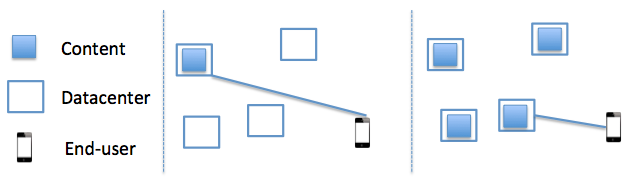
\includegraphics[scale=0.5]{fig/placement-vs-redirection.png}
	\caption{Placement vs. redirection: Content placement creates options for the redirection scheme to choose a nearby location for reducing user-perceived latencies.}	
	\label{fig:placement-redirection}
\end{figure}


\textbf{Placement vs. redirection:} Among the set of locations with the content, redirection chooses a location to send request. If the content is placed only at a far-away location, irrespective of how redirection is done, a user will observe a high latency to fetch content from the remote location. On the other hand, content placement can create more options to the redirection scheme to choose a location that is nearby. Thus, effective placement is a pre-requisite for a redirection scheme to provide low latencies.


%We briefly explain the \emph{traffic engineering} problem that is pertinent to our discussion of placement vs. routing. Traffic engineering computes network routing based on inputs of are the network topology, link capacities, and a \emph{traffic matrix}. A traffic engineering scheme computes routing to satisfy traffic demands while optimizing a cost function dependent on link utilization. For example, a common cost function is the maximum link utilization, MLU \cite{rexford}. 


\textbf{Placement vs. routing:} Content placement is more powerful than routing because it can change the \emph{traffic matrix} for which the routing is to be computed. A traffic matrix is a 2-dimensional matrix representing the demand in the network. The $i,j$-th entry in this matrix is the traffic from node $i$ to node $j$ in the network topology \cite{fortz2000internet}.  Let us take an example traffic matrix for which routing is to be computed (Figure \ref{fig:placement-routing}). Content placement can turn any non-zero traffic matrix into a null matrix (one whose all entries are zero) provided all content that a node in a network needs is placed at the same node. Such a placement obviates the need to send traffic to any other node, and therefore makes routing a trivial problem. While this is an extreme example, and one may not have sufficient resources to place content at all locations in the network, this example demonstrates that the ability to change the traffic matrix makes content placement more powerful than routing.

\begin{figure}
	\centering
	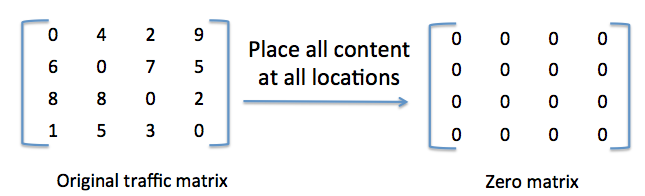
\includegraphics[scale=0.4]{fig/placement-vs-routing.png}
	\caption{Placement vs. routing: content placement is more powerful than routing since it can change the  traffic matrix itself.}
	\label{fig:placement-routing}
\end{figure}


\section{Research overview}

The research in this thesis is categorized into three topics: 

(1) Traffic engineering is an important task for network operators and is responsible for cost and congestion reduction and fault tolerance \cite{rexford,COPE,TEXCP}. While traditionally traffic engineering is viewed as a routing problem, we study the role of content placement in shaping traffic engineering objectives in content-dominated networks.

(2) The lack of support for handling mobility in the Internet is well-documented \cite{HIP,LISP,HAIR,MobilityFirst}. Towards building infrastructure support for mobility in the Internet, we present the design and implementation of Auspice global naming service that meets the scalability and consistency requirements posed due to high mobility.

(3) To reduce the energy use of datacenters used for storing and serving content, we design and implement a system shrink that uses server consolidation and content migration to reduce energy use while meeting operator-specified service level agreements.


\subsection{Traffic engineering in content-dominated networks}

Traffic engineering in ISP networks is not isolated from decisions at the application layer.
The primary goal of traffic engineering is to configure network routing to reduce capacity provisiong costs as well as network congestion.
But, in a content dominated network, traffic engineering interacts with content placement and request redirection. The over-arching goal of our work is to design and evaluate ISP traffic engineering techniques while accounting for their interaction with content placement and request redirection. 

We address the above question in two scenarios. The first scenario in a more common occurence in present day Internet, in which an ISP has little control over placement and redirection. The second scenario is motivated by a recent, potentialy transformative trend: Network CDNs (NCDNs) -- CDNs deployed by ISPs on their infrastructures. Unlike traditional ISPs, an NCDN enjoys full control over placement, redirection and routing on its network.

\subsubsection{ISP network with content location diversity}

We model a content-dominated ISP network by accounting for its content \emph{location diversity} -- the presence of content at multiple network locations, and the ability of end-users to download content from those locations. Location diversity is enabled by several types of applications and services, such as CDNs, P2P, mirrored websites. We create location diversity using a simple content placement scheme -- randomly placing content at multiple locations --, to reflect the limited control of ISPs on content placement in their networks. 

%We further assume that users can download content in parallel from all locations. 

Our work presents an experimental comparison of several classes of traffic engineering schemes using data from real ISP topologies and traffic matrices. Our key findings are as follows: (1) We find that all traffic engineering schemes, including shortest-path routing, multiprotocol label switching routing, routing that is robust to unpredictable variations as well as optimal traffic engineering, achieve similar application performance and network capacity.   (2) We find that even a static shortest-path routing, or in other words a ``no'' traffic engineering  scheme is at most 30\% sub-optimal in terms of network capacity. Overall, these results suggest that even a limited placement flexibility reduces the value of sophisticated traffic enginering schemes, e.g., optimal traffic engineering, over simpler traffic engineering schemes, e.g., shortest path routing. These results are further strengthed in the case of a network CDN where the content placement flexibility is even greater.


\subsubsection{Network CDNs}

There are strong economic factors motivating ISPs to transform into network CDNs for delivering content to users on its network: falling bandwidth prices due to competition and technology trends, potential sources of revenue by selling content-based services to end-users, easy availability of CDN technology in the form of licensed and managed CDNs and reduction in backbone traffic due to content caching via NCDNs are some of the most prominent factors \cite{telco-cdn-arguments}. Today, more than 30 ISPs have deployed NCDNs. 

NCDNs represent a paradigm shift in which both content delivery and traffic engineering is handled by a single entity. 
A natural question is to ask how should NCDNs handle placement, redirection and routing for optimize traffic engineering objectives such as maximum link utilization, as well content delivery objectives such as user-perceived latency. Accordingly, our work evaluates several combinations of placement and routing schemes that an NCDN can deploy. First, a simple caching scheme for placement and a static-shortest path routing. Second, a joint optimization of placement and routing based on historic demand patterns. Third,  an ideal joint optimization with future knowledge of content demand.  Of particular interest to NCDNs are demand-oblivious schemes such as the first scheme, as they make placement and routing decisions without measurement of content demand and simplify network management for the operators.

Our key findings, based on real network topologies, and extensive traces from Akamai CDN, demonstrate the effectiveness of a demand-oblivious scheme. First, due to poor predictability of content demand and the churn in content workloads, a scheme that optimizes placement, redirection and routing jointly based on historical content demand performs much worse than the simple demand-oblivious scheme. Second, the demand-oblivious scheme performs close to an ideal joint-optimization strategy with knowledge of future content demand, largely because the caching scheme achieves high cache hit rates from caches placed inside the network.  Third, optimizing routing matters little in NCDNs: whether a static shorted-path routing or a routing optimized based on measured traffic demands is used along with a caching scheme, the network cost differs by less than 10\%. 


\textbf{Summary:} ISPs have traditionally focused on optimizing routing to achieve their objectives, but our research shows that in a content-dominated network, they are better served by leveraging placement flexibility using simple placement schemes.


\subsection{Global name service for highly mobile Internet}


Internet's poor support for mobility is visible at several corners: 

A key reason for Internet's poor support for moblity is that communication on the Internet is based on IP addresses that keep changing due to mobility. On the other hand, what remains unchanged is the name or identity of communication end-points. If we can enable communication over names, we can handle mobility. A  global name service (GNS) handle mobility maintaining an up-to-date mapping from names to network addresses for all names. If such a GNS were to exist, an end-point Alice would be able to establish a connection with another end-point Bob by querying the GNS for Bob's adresss as shown in Figure \ref{fig:gns-example}. 

\begin{figure}
	\centering
	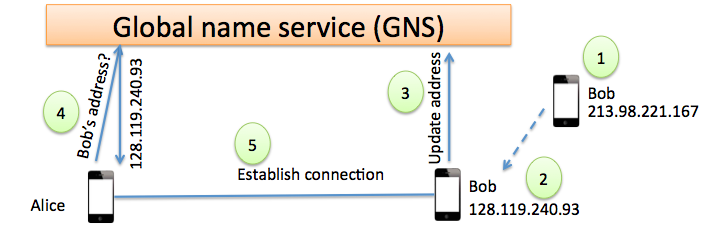
\includegraphics[scale=0.4]{fig/gns-example.png}
	\label{fig:gns-example}
	\caption{A global name service helps establish and maintain connections between mobile entities by keeping an up-to-date mapping from their names to their network addresses.}
\end{figure}

To appreciate the challenges in implementing such a GNS, we discuss the limitation of Internet's existing naming service DNS as a solution for mobility.
\begin{enumerate}
	\item DNS relies heavily on passive caching based on TTLs for reducing both system load and client-perceived latency. However, high mobility severely limits effectiveness of TTL-caching. Handling mobility requires up-to-date responses, so the load and client-perceived latency increase with the mobility rate irrespective of the TTL.
	\item Under high mobility, the latency to an authoritative name server determines client-perceived query latency in the common case. Today, authoritative name server locations are chosen statically irrespective of where the query demand is coming from, which could results in highly sub-optimal query latencies. 
	\item Due to DNS's hierarchical design, the implementation of DNSSEC extensions for DNS's security depends on a single root of trust, a root that is tightly controlled today by ICANN and the US Department of Commerce, a state-of-affairs that is inherently anti-competitive and geo-politically problematic. 
\end{enumerate}

Our work makes two main contributions towards addressing the challenges of designing a global name service for high mobility. 

\textbf{Global naming system:} We present a clean-slate naming system design that is incompatible with existing DNS but improves upon DNS's design in two aspects. First, it supports multiple roots of trust as a part of the naming system, thereby addressing the single root of trust problem in DNS. Second, it supports name-to-address resolution for arbitrary names unlike DNS, which restricts names to be hierarchical. In doing so, our naming system gives applications the full flexibility in choosing names. 

\textbf{Auspice name resolution service:} A key component of our naming system is Auspice: a scalable geo-distributed service for mapping names to network addresses under high mobility. A key decision in Auspice's design is that of placement of name records that store the name-to-address mapping. The placement problem is challenging due to a fundamental cost-vs.-performance trade-off: placing name record at multiple locations improves latency of content accesses but increases update propagation costs. To address this challenge, Auspice name resolution service infers pockets of high demand for a name and uses a heuristic placement strategy that selects both the number and location of the replicas in a demand-aware manner to provide low request latency, low update cost, and high availability.  We extensively evaluate Auspice for an expected workload of a global name service and show that it significantly outperforms both commercial managed DNS services as well as DHT-based replication alternatives to DNS. Auspice is deployable in the Internet today as a scalable managed DNS provider, potentially enhacing support for mobility in the present day Internet as well.

\subsection{Energy optimization in content datacenters}
Energy use is a key component of operational costs of \emph{content datacenters (CDCs)}, datacenters that are used for storing and serving content to end-users. CDCs can potentially reduce their energy use via consolidation of servers and switches, but in doing so, they risk inflating end-user response times potentially leading to SLA violations. Our primary contribution is to quantify the tradeoff between energy savings via consolidation and response times in CDCs, and the design and implementation of Shrink, a system that aggressively leverages this tradeoff in order to yield significant savings in energy use in CDCs while affecting user-perceived response times in a controlled manner. To our knowledge, Shrink is the first system to consolidate servers and switches in a coordinated manner, an approach that reduces network energy use by up to 42\% compared to network-unaware server consolidation schemes. Our evaluation of Shrink using a workload from a large CDN's datacenter shows that Shrink can reduce energy use by 35\% over a scheme provisioned for the peak demand, while increasing the mean, 95th and 99th percentile response times by 8\%, 3\% and 15\% respectively.



\section{Thesis organization}

The thesis is organized intro three parts in correspondence with the three topics of our research.

Chapter \ref{ch:te-background}, Chapter \ref{ch:beyondmlu} and Chapter \ref{ch:ncdn} present our research on traffic engineering in content-dominated networks. Chapter \ref{ch:te-background} presents background on traffic engineering, content delivery and the interaction between them. Chapter \ref{ch:beyondmlu} presents a comparison of traffic engineering schemes in a network with location diversity of content. Chapter \ref{ch:ncdn} designs and evaluates traffic engineering and content delivery schemes in a Network CDN.

Chapter \ref{ch:intro-auspice} presents the design, implementation and evaluation of a global name service for a highly mobile Internet.

Chapter \ref{ch:shrink} presents the design, implementaiton and evaluation of Shrink - a system for reducing energy use of content datacenters via server consolidation.

\section{Previous publications and collaboration}

\textbf{Chapter \ref{ch:beyondmlu}} revises a previous publication: A. Sharma, A. Mishra, V. Kumar, A. Venkataramani. Beyond MLU: An Application-Centric Comparison of Traffic Engineering Schemes. \emph{Proc. IEEE INFOCOM, April 2011}. Aditya Mishra and Vikas Kumar provided invaluable support in performing experiments for this work.

\textbf{Chapter \ref{ch:ncdn}} revises a previous publication: A. Sharma, A. Venkataramani, R. Sitaraman. Distributing Content Simplifies ISP Traffic Engineering. \emph{Proc. ACM SIGMETRICS, June 2013}. Ramesh Sitaraman provided access to Akamai datasets for this work. A realistic experimental evaluation would not have been possible without these datasets.

\textbf{Chapter \ref{ch:intro-auspice}} revises a previous publication: A. Sharma, X. Tie, H. Uppal, D. Westbrook, A. Venkataramani, A. Yadav. A Global Name Service for a Highly Mobile Internetwork. \emph{Proc. ACM SIGCOMM, August 2014}. 
This work also appears in Xiaozheng Tie's thesis, which describes the same placement algorithm and a simulation-based evaluation of the algorithm. The new material in this chapter includes (1) mechanisms to provide consistency of data and (2) experiments with an implementation of the placement algorithm in an emulation testbed and a geo-distributed testbed. Both Xiaozheng Tie and Hardeep Uppal have contributed to the placement algorithm. Hardeep Uppal, David Westbrook and Arun Venkataramani have contributed in implementing the \auspice\ system.


%%!TEX root = Main.tex
\vsp
\section{Introduction}
\label{sec:intro}
``Mobile'' has long arrived, but the Internet remains unmoved. Today, there is roughly one cellphone per human; the number of smartphones sold last year alone roughly equals the number of wired hosts on the Internet \cite{gartner}; and the total traffic originated by mobiles is poised to approach that by wired devices \cite{cisco-vni}. However, the current Internet continues to operate as it did when dominated by tethered hosts, simply ignoring frequent endpoint mobility.

Today, an application developer can not easily initiate communication with a smartphone even when it has a public IP address as there is no global infrastructure support for locating it. Applications like smartphone notification systems, playback video, or cloud storage have to develop application-level support to enable a seamless experience for their users even as they change addresses several times a day, or let connections break (as popular VoIP apps do today).   The lack of intrinsic support for mobility means that developers are forced to redundantly develop and maintain common-case functionality. Furthermore, we are paying an unknowable price in terms of long-term growth and innovation by straitjacketing communication initiation to be unidirectional.

%The lack of intrinsic support for mobility means that we are paying an unknowable price in terms of stymied application innovation and growth by forcing developers to redundantly develop common-case functionality, and forcing communication initiation to be mostly unidirectional.

%A mobile user might reasonably expect that a voice-over-IP call she initiated through one WiFi network would continue uninterrupted if she switched to a different WiFi or  cellular network; or expect a file transfer she initiated at home on her laptop to resume when she opens it at work in a disruption-tolerant manner. Today, one can not easily initiate communication with a smartphone (even when it has a publicly visible IP address) because there is no global infrastructure support for locating it. Of course, application developers can design around these limitations, as do applications like Skype\tbd{I don't think Skype actually supports this today. Netflix maybe a better example.}, Dropbox, and smartphone notification systems respectively for the above scenarios. However, the lack of intrinsic support for mobility means that we are paying an unknowable price in terms of stymied application innovation and growth by forcing developers to redundantly develop common-case functionality, and forcing communication initiation to be mostly unidirectional.

%Many before us have criticized the Internet architecture's poor support not only for mobility but also for multihoming \cite{HIP,LISP,HAIR}, content retrieval \cite{DONA,LNA,CCN}, and security \cite{AIP,XIA,MobilityFirst-UMASS}. A common criticism is the Internet's so-called conflation of identity and location. The Internet uses an IP address both to represent the identity of an interface as well as its network location, which is problematic for mobility (same identity, changing locations) and multihoming (single identity, multiple locations) of devices, services, or content. Applications today are forced to know and care about changing IP addresses as the transport and network layers only provide a primitive to establish  connections between IP addresses, not application-friendly names. It is commonly accepted wisdom that a cleaner separation of identity and location is instrumental to fixing these problems.

%Many before us have criticized the Internet architecture's poor support not only for mobility but also for multihoming \cite{HIP,LISP,HAIR}, content retrieval \cite{DONA,LNA,CCN}, and security \cite{AIP,XIA,MobilityFirst}. A common criticism is the Internet's so-called conflation of identity and location. The Internet uses an IP address both to represent the identity of an interface as well as its network location, which is problematic for mobility (same identity, changing locations) and multihoming (single identity, multiple locations) of devices, services, or content. Applications today are forced to know and care about changing IP addresses as the transport and network layers only provide a primitive to establish  connections between IP addresses, not application-friendly names. It is commonly accepted wisdom that a cleaner separation of identity and location is instrumental to fixing these problems.

Many before us have criticized the Internet architecture's poor support for mobility as well as multihoming \cite{HIP,LISP,HAIR,MobilityFirst}. A common criticism is the Internet's so-called conflation of identity and location, i.e., the use of an IP address both to represent the identity of an interface as well as its network location, which is problematic for mobility (same identity, changing locations) and multihoming (single identity, multiple locations). It is commonly accepted wisdom that a cleaner separation of identity and location is instrumental to fixing these problems. However, the Internet does separate identities (domain-names) from network locations (IP addresses) through DNS. Most high-level programming languages also provide syntactic sugar to \verb+connect+ to names remaining oblivious to IP addresses; and %name owners can and do employ managed DNS services or CDNs to return the best-positioned network location corresponding to multi-homed names. 
techniques from a long line of work on connection migration could be employed to seamlessly handle mid-connection mobility.

But a key missing element from this package today is a distributed name resolution infrastructure that can scale to orders of magnitude higher update rates than envisioned when DNS was created. To appreciate the envisioned scale, consider tens of billions of mobile identifiers changing network addresses at least tens of times per day. DNS's heavy reliance on TTL-based caching, a key strength recognized by its creators, researchers, and operators alike, poses a significant handicap by increasing update propagation delays, load on name servers, and overall client-perceived latency. It is not uncommon for DNS update propagation to take a day or more, resulting in long  outage times when online services have to be moved unexpectedly, prompting cries for help on operator forums \cite{serverfault,dns-long-update}. A less widely noted limitation of DNS is its reliance on hierarchical names for scaling via federation and its single root of trust, which constrains mobile applications from selecting arbitrary application-specific names (as elaborated in $\S$\ref{sec:whyNotDNS} and $\S$\ref{sec:design_overview}).

 %   Mobile has arrived, but the Internet is still static.

%    Reason 1: identity-location conflation. A number of solutions proposed to address this.

%    Reason 2: identity-location conflation would not be that problematic with an efficient resolution infrastructure. The Internet does separate human-readable ``names" from ``locations" or IP addresses through DNS. However, the design of the DNS resolution infrastructure implicitly assumes rare mobility. Indeed, Mockapetris and Dunlap allude to this by justifying the design decision of departing from the Xerox PARC Grapevine system... quote here.


Our position is that seamless support for mobility requires a logically centralized global name service that rapidly translates identities to locations irrespective of how exactly identities and locations are individually represented. Our primary contribution is the design, implementation, and evaluation of \auspice, a distributed system that helps address this challenge. Compared to today's ICANN/DNS-based approach, our approach cleanly separates name resolution from adjudication and certification issues ($\S$\ref{sec:design_overview}). \auspice\ is also deployable as a managed DNS provider in today's Internet; compared to them, a key strength of \auspice\ is a {\em demand-aware} replica placement engine that significantly reduces the {\em time-to-connect} to mobile destinations in a cost-effective manner. Under light load, \auspice's demand-aware replica placement aggressively uses available resources to massively replicate name records, while under heavy load, it carefully controls the number and choice of replica locations based on the read-write patterns and pockets of high demand for each name.

%low lookup latency, low update cost, and high availability.  \auspice\ achieves low-latency by inferring pockets of high demand for a name so as to create replicas of  for that name close to them. \auspice\ achieves low latency,  low update cost,  and high availability using a placement optimization algorithm that (1) controls the number of replicas based on the observed read and write rates, and (2) determines where to place replicas based both on the inferred pockets of demand and the aggregate load at node locations near those pockets. 



We have implemented a prototype of \auspice\ as a geo-distributed key-value store to serve as a flexible name resolution service for the current Internet as well as several ``future'' Internet or endpoint architectures such as MobilityFirst\cite{MobilityFirst}, HIP\cite{HIP}, or XIA\cite{XIA}. We have extensively evaluated \auspice\  using a combination of Planetlab, emulation clusters, and Amazon EC2.  Our contributions are as follows.
\begin{enumerate}
\item A case for a global name service as an indispensable part of any Internetwork design with intrinsic support for high mobility ($\S$\ref{sec:case}).
\vsp
\item \auspice, a scalable, geo-distributed, federated global name service that significantly reduces the time-to-connect under any given resource constraints despite high mobility and arbitrary endpoint identifiers ($\S$\ref{sec:design},$\S$\ref{sec:eval}). 
\figvsp
\item A proof-of-concept demonstration of intrinsic support for---{\em(i)} all four types of endpoint mobility; {\em(ii)} novel context-aware delivery primitives that generalize name- or address-based communication---over the current Internet as well as MobilityFirst \cite{MobilityFirst} ($\S$\ref{sec:e2e}). 
\vsp
\item Comparison against several best-of-breed managed DNS services showing that \auspice's  demand-aware approach significantly lowers time-to-connect and/or update cost even for today's (hardly mobile) domain names ($\S$\ref{sec:managed}).
\vsp
\end{enumerate}
\vsp

To provide a historical perspective, until the early 80s, the Internet relied on a system called \verb+HOSTS.TXT+ for name resolution, which was simply a centrally maintained text file distributed to all hosts. The current Internet's distributed DNS  arose in response to the rapidly increasing file size and distribution costs. Mockapetris and Dunlap \cite{DNS} point to TTL-based caching to reduce load and response times as a key strength, noting that ``{\em{the XEROX system {\em [Grapevine \cite{grapevine}]} was then ... the most sophisticated name service in existence, but it was not clear that its heavy use of replication, light use of caching ... were appropriate}}''. We have since come a full circle, turning to  active replication ($\S$\ref{sec:whyNotDNS}) in \auspice\ in order to address the challenges of mobility, a concern that wasn't particularly pressing  in the 80s. Compared to classical systems like Grapevine or ClearingHouse, \auspice\ enables support for automated {\em demand-aware} replica placement for {\em arbitrary names} (using several modern design elements such as consensus, the key-value abstraction, self-certifying names, consistent hashing, etc).  \auspice, through its support for context-aware delivery, is also a step towards addressing some of the challenges to which Lampson alludes on representing ``descriptive names" \cite{Lampson}.


\eat{
\emph{Low update cost:} \auspice\ reduces updates costs by nearly an order of magnitude over a replicate-everywhere strategy in a live deployment and yet achieves nearly identical lookup latencies.
\item
\emph{Load balance:} Over a wide range of loads, \auspice's achieves 2X - 4.5X lower lookup latencies over a random replication scheme, and  5.4X - 11.2X lower latency than a DHT-based replication scheme. Due to its lower update costs, \auspice\ can sustain 18$\times$ higher loads than a replicate everywhere strategy.
}

%\begin{itemize}
%\item
%Locality-aware placement helps \auspice\ achieve 5$\times$ lower median lookup latency than a DHT-based replication scheme. 
%\vspace{-0.1in}
%\item
%\auspice\ reduces updates costs by nearly an order of magnitude over a replicate-everywhere strategy in a live deployment and yet achieves nearly identical query latencies.\vspace{-0.1in}
%\item
%\auspice's load-aware design achieves 1.2$\times$-3.3$\times$ lower lookup latencies than a locality-unaware scheme over a wide range of load scenarios.\vspace{-0.1in}
%\item
%\auspice\ achieves  DNS lookup latencies comparable to a leading managed DNS provider today even with only one third the number of name resolvers.
%\end{itemize}

%\begin{enumerate}
%\item  \auspice's locality-aware and load-aware replication achieves  5$\times$ lower latency than Codons, a proposed DHT-based replication alternative to DNS.
%\item \auspice\ reduces update costs
%\end{enumerate}
\eat {

The Internet's tremendous success and our maturing realization of its shortcomings have attracted significant research attention towards a clean-slate redesign of the Internet's architecture (e.g., NSF FIND \cite{FIND}, GENI\cite{GENI}, FIA\cite{FIA}). A number of the shortcomings of the current Internet can be traced back to issues related to {\em naming}, a central component of any distributed system design. In the current Internet, network entities are identified using IP addresses and the Domain Name System (DNS) resolves human-readable end-host names to IP addresses. Although this design has proven to be surprisingly malleable, it suffers from two sets of fundamental problems, both of which are  exacerbated by the the exponential growth of mobile devices and applications today.


The first results from the conflation of identity and location within an IP address, a design decision roundly criticized by many \cite{ROFL,Saltzer:1993:NBN:RFC1498,HIP,FARA,LNAI}. Using an IP address to identify a network interface as well as the network location of that interface complicates {\em mobility}---when the location changes but not the identity---and {\em multihoming}---when a single identity simultaneously resides at multiple locations---e.g., being simultaneously connected to a cellular and WiFi access network. With roughly 5 billion mobile devices worldwide today \cite{gartner}  (over a billion of which are IP-capable) compared to barely a billion tethered hosts \cite{CIA}, mobility and multihoming are the norm, not an exception. Conflating identity and location also poses a serious but  less widely acknowledged security challenge, namely, verifying that an interface indeed has the identity it claims. Unlike human-readable names that are bound to public keys by trusted certification authorities in order to enable application-level authentication today, IP addresses are harder to certify, especially when they change many times a day. As a result, we largely make do today with application-level security over a network that can be easily rendered unavailable by spoofing or hijacking of IP addresses.



The second results from the architecture of DNS, a critical part of the Internet's core infrastructure. The design of DNS in the Internet's early days implicitly assumed tethered hosts or infrequently changing addresses to be the common case, an assumption evident in its heavy reliance on caching and timeout-based invalidations for scalability. An inevitable consequence of this design is that unanticipated updates to DNS resource records are slow; more than 40\% domain names have a TTL of a day or more \cite{codons}. Even for slow-changing records, DNS lookup times constitute a significant fraction of user-perceived response times, e.g., over 30\% of web objects incur a DNS lookup latency of over a second \cite{Jung,Huitema}. Deploying more passive local name sever caches can reduce lookup latencies, but this benefit comes at the cost of further increasing update propagation delays or update load in the system. These and other problems with DNS such as poor load balance and responsiveness to changing demand patterns, vulnerability to denial-of-service attacks, etc. have been well documented by researchers \cite{Pappas,codons,Brownlee,dnssec}.

Our primary contribution is the design and implementation of a global name service that addresses the above problems. This global name service is a central component of MobilityFirst, a clean-slate future Internet architecture that is primarily motivated by the dual concerns of {\em mobility} and {\em security}.
%two concerns that are remarkable both for their absence in the design philosophy underlying the current Internet \cite{Clark88} as well as their immense importance today. 
MobilityFirst cleanly separates identity and location using a {\em globally unique identifier} (GUID) that, unlike an IP address, is by design devoid of location or any other structured information. Information about a GUID's location or {\em network address} (NA) is maintained by the resolution service. Both GUID and NA are {\em self-certifying}, i.e., they are one-way hashes of public keys, allowing any network entity to authenticate an entity claiming to possess a GUID or NA. Thus, the structureless nature of these identifiers enhances mobility as well as security. Section \ref{sec:MF} describes how the name service helps efficiently support a number of other functions such as multihoming, incoming traffic engineering, content retrieval, network mobility, multicast, etc.

%Key feature: low response times while respecting capacity constraints and consistency requirements. TBD.

A critical distributed systems challenge in realizing a global name service that supports mobility at scale  is the design and implementation of the infrastructure that quickly resolves identifiers to network addresses. To appreciate the scale, consider 10 billion identifiers (for mobile devices, services, content identifiers, or entire networks such as vehicular networks) moving across a 100 network addresses per day, i.e., a load of a million/sec for updates alone. Furthermore, the name service should process lookup queries quickly, requiring queries to be directed to a nearby replica that holds a consistent replica of the corresponding resource records. Finally, the service should balance the aggregate load across all names across the geographically distributed locations of the global name service. 

Our proposed solution to achieving all of the goals above---low latency, low update cost, and load balance---is a placement engine \auspice, that {\underline{\bf au}}tomates {\underline{\bf s}}ervice {\underline{\bf p}}lacement {\underline{\bf i}}n {\underline{\bf e}}lastic {\underline{\bf c}}louds. The \auspice\ engine is flexible in that it enables automated placement for cloud-hosted services that are more general (and in widespread use today) than name resolvers in a future Internet architecture. To ensure low response times, \auspice\ dynamically spawns or migrates service replicas close to pockets of high demand. To ensure low update cost and load balance under capacity constraints, \auspice\ controls the number and placement of service replicas using heuristic algorithms that are uncoordinated across services or a global optimization algorithm coordinated across all services by the hosting service provider.

We comprehensively evaluate \auspice\ using an implemented prototype on Planetlab and Amazon EC2. Also design custom simulator. Validate simulator. Case studies and results preview. TBD.

\paragraph{Roadmap} The rest of this paper is organized as follows. Section \ref{sec:MF} presents the naming subsystem in the MobilityFirst Internet architecture. Section \ref{sec:auspice} presents the design goals and architecture of an automated service replica placement system, \auspice, for geo-distributed cloud-hosted services and the instantiation of a global name service using it. Section \ref{sec:eval} describes the datasets used and the experimental evaluation of \auspice. Section \ref{sec:related} describes related work and Section \ref{sec:concl} concludes.

}

%
% We study  \emph{role of content placement strategies on interaction between networks and content delivery systems}, as aspect which has received little attention in prior work in this area. We find that content placement is a strong factor in shaping the flow of  traffic in the network, e.g, placing content at a large number of locations results in localized traffic flows. By choosing the placement strategies suitably, network traffic can be shaped to optimize the objectives of both content delivery systems, e.g., minimizing the latency of files transfers, as well as networks, e.g., minimizing the utilization of links in the network. Further, we show that simple placement schemes are effective in improving cost-, performance- and energy-related metrics for networks and content delivery systems.


%Our goals are to shed light on the role of content placement strategies on interaction between networks and content delivery systems and enhance network architecture support for end-host mobility.

First, and the more pronounced theme, is studying the \emph{role of content placement strategies on interaction between networks and content delivery systems}, as aspect which has received little attention in prior work in this area. We find that content placement is a strong factor in shaping the flow of  traffic in the network, e.g, placing content at a large number of locations results in localized traffic flows. By choosing the placement strategies suitably, network traffic can be shaped to optimize the objectives of both content delivery systems, e.g., minimizing the latency of files transfers, as well as networks, e.g., minimizing the utilization of links in the network. Further, we show that simple placement schemes are effective in improving cost-, performance- and energy-related metrics for networks and content delivery systems.

Second, is \emph{enhancing network architecture support for end-host mobility}.  Today, content delivery systems need to work around the problem of being unable to initiate and maintain connections to mobile hosts by building application-level mechanisms such as push notification services. Our position is that end-host mobility can be seamlessly handled with the support of a global name service that translates host names to their network address under frequent  mobility of end-hosts.  To this end, we present the design, implementation, and evaluation of Auspice, a scalable, geo-distributed name service.  A key decision for this service, affecting both performance and update costs, is the placement of name records of mobile hosts. Auspice infers pockets of high demand for a name and uses a heuristic placement scheme to provide low address lookup latency, low update cost, and high availability. Our evaluation of Auspice's implementation  shows that Auspice significantly outperforms both commercial managed DNS services as well as DHT-based replication alternatives to DNS.


%Our key insight is that interactions between networks and content delivery systems depend strongly on content placement strategies. The locations at which content is placed in the network shapes the flow of  traffic in the network, e.g, placing content at a large number of locations results in localized traffic flows. By choosing the placement strategies suitably, network traffic can be shaped to optimize the desired objectives of content delivery systems, e.g., minimizing the latency of files transfers, as well as networks, e.g., minimizing the utilization of links in the network. 

%This thesis also investigates services a network can offer that are useful in designing content delivery systems.  Much prior research in network architecture has proposed several such services such as QoS, IP multicast, Name-based routing. There is a long list of  possible services and diverse mechanisms are needed to support all of them. Therefore,  we focus on the problem of handling end-host mobility in the Internet, a pressing problem for modern-day Internet in which devices are predominantly mobile, and traffic generated to or from mobile devices is the majority of traffic in the Internet. 


%Therefore, effective content placement not only improves cost and performance metrics of the content delivery systems, but also of the underlying network. 


%This phenomenon implies that networks have an additional knob, in the form of content placement, to 

%Therefor,
%

%Networks have traditionally relied  optimized  routing optimizations 
%Thus content placement provides an additional knob 
%
%While networks have traditionally depended on routing optimizations 
%An implication of this phenomenon is that content placement can be leveraged by the underlying network to 




**************************************************************


 We study the interaction between networks and content delivery in three domains, and find that 
content placement is a strong factor in shaping the flow of  traffic in the network and that simple placement strategies 


 Further, content delivery systems and networks affect each other's decisions in trying to shape the flow of traffic with their respective techniques. Therefore, content delivery systems, networks, and the interaction between the them, all play a role in determining user-perceived performance in the Internet. 



The design of content delivery systems depends on 



As content delivery systems and networks are often under the control of distinct, non-cooperating entities in the Internet, work in one area has largely ignored any interactions with another.

Yet, content delivery systems and networks affect each other's decisions in trying to shape the flow of traffic with their respective techniques. 




A network architecture influences on the design on content delivery systems. 


Networks influence content delivery 

The decisions by networks and content delivery systems 

Both networks and content delivery systems shape the flow of traffic in the network, 

Content delivery systems and networks influence each other's decisions. How?

As content delivery systems and networks are often under the control of distinct, non-cooperating entities in the Internet, work in one area has largely ign


Work in content delivery systems, 



The design and performance of content delivery systems depends on the services that underlying network offers and on network routing decisions.
Reciprocally, content delivery systems affect network routing decisions as they shape the flow of traffic in the network to optimize end-user performance. 
Still, work in content delivery systems and networks has largely ignored the interactions with another, because content delivery systems and networks are often under the control of distinct, non-cooperating entities in the Internet.
The goal of this thesis is to enhance and leverage these interactions to improve cost-, performance-, and energy-related metrics for networks and content delivery systems.


Content delivery systems and networks are often under the control of distinct entities in the Internet. 
As a result, work in content delivery systems and networks has largely ignored the interactions with one another. 
Yet, content delivery systems and networks affect each other's decisions.


 

We consider two approaches for how these interactions occur and how they are leveraged. 

There are two key ideas (1) leveraging the flexibility to place content 

(2) enhancing 

as their respective optimizations 

Content delivery systems and networks both affect each others decisions. 

The services offered by the underlying network 

We consider two forms of interactions between networks and content delivery systems as described below. 

(1) interaction between network route optimization and content delivery decisions such as content placement and request redirections 

(2) how content delivery systems are designed depends on the services offered by the underlying network.




Interaction between networks and content delivery occurs 

This thesis considers two forms of interactions between networks and content delivery. First, 


How content delivery systems are design and 

Content delivery systems rely on connectivity provided by the underlying networks to reach the  

Networks provide the connectivity between hosts across and content delivery systems operate an overlay across 

\begin{enumerate}
\item

*** get feedback from people ***

*** self-revealing bullets ***
\textbf{what is a content delivery network}


*** network CDNs ***
The idea of \emph{content delivery} using a network of distributed caches was pioneered by Akamai in 1990s. Since then, Internet has seen a proliferation in the number of CDNs and their customers and nearly every major web service today relies on a content delivery infrastructure to ensure a high quality experience for its end-users. A typical CDN  operates a set of distributed server deployments, and uses a combination of edge caching, intelligent request redirection, and path and protocol optimizations for delivery of several types of content, e.g., video, bulk downloads, and interactive websites. 

%This thesis takes a broad view of a content delivery network including edge caches and origin servers, and  global and regional CDNs, e.g., a network CDN delivering content to users on its network.

\item
\textbf{content delivery systems need  high performance and cost-effective designs}

Content-delivery networks (CDNs) have always sought to provide a high-quality user experience in a cost-effective manner. Yet, better performing and more cost-effective systems are as relevant for CDNs today as ever, due to following reasons:
(1) Several recent studies have shown that CDNs have potential to attract more traffic by improving the user-perceived performance.
(2) CDN marketplace has seen many new entrants in recent years due to commoditization of CDN technology, which has resulted in increased pressure on CDNs to reduce costs.
(3) CDNs cannot rely on improvements in hardware alone to reduce costs because the size of new content generated and accessed by end-users has outpaced the hardware growth in the last five years, e.g. online video traffic has increased by X hundred\% in last five years and is projected to do so in next 10 years.


%CDNs have more pressure to reduce costs today than  in order to stay competitive in a marketplace that has seen many new entrants in recent years.

%CDNs have increased pressure to reduce costs in order to stay competitive in a marketplace that has seen many new entrants in recent years. Due to these trends,  better performing and more cost-effective systems are as relevant for CDNs today, as ever. 


\item
\textbf{ideas: exploit locality using placement, use planned for predictable workloads}

This thesis uses two key ideas in designing high-performance and cost-effective solutions for CDNs: *** don't introduce terminology *** exploiting workload locality with  suitable placement algorithms (2) for workloads that are predictable over long periods, using a planned approach, i.e., making decisions using analysis of past workloads, to get better results. These ideas have been used in designing CDNs and distributed systems in general. Our contribution is to show application of these ideas in new problem domains and to improve state-of-the-art solutions as described in Section \ref{sec:contribution}. 
We elaborate on these ideas below.


\item
\textbf{content placement is key factor in affecting cost and performance}

User-perceived performance and costs of a CDN depend to a great extent on the content placement algorithms. Placing a content at multiple locations  improves the user-perceived performance but increases infrastructure and operational costs of content delivery system, e.g., placing of large video at multiple locations increases the storage requirements of the system;, placing dynamic objects at multiple locations is associated with costs of propagating updates to all locations; for a CDN that operates its own network, the placement algorithm affects how much traffic is carried by network links hence influences the network costs. 

*** placement, network-effect, ****

*** buzzwords: select buzzwords and use it over and over. ****

CDNs and end-users cooperate 

%Cost-effective and high performance designs can be achieved by leveraging geographical and temporal locality in request patterns by a suitably choosing the placement algorithms.



%Costs incurred by CDNs are mainly due to the costs of replicating objects at multiple locations. 

\item
\textbf{content placement exploits locality to improve cost and performance}

Intelligent content placement strategies would be of limited use in designing high performance, cost-effective solutions for CDNs if  there was no geographic and temporal locality to requests.  Real workloads do show geographic and temporal locality patterns as is shown in experiments in this thesis as well as in several measurement studies of web, video, and social networking traffic. Intelligent placement strategies can exploit the locality in workload by placing objects, at those times and locations, where the content is highly popular. Thus, an effective placement policy can enable a CDN to limit the cost of replicating objects, and improve user-perceived performance. 



\item
\textbf{Design space: planned and unplanned schemes}

We consider two broad classes of solutions in this thesis: \emph{planned}  and \emph{unplanned}.
%This thesis studies two approaches to resource management: \emph{planned} and \emph{unplanned}. 
A planned approach assumes that  workloads in future will resemble those in the past, and makes decisions including those of  placement, redirection,  routing, and bandwidth allocation using an historical knowledge of workloads. An unplanned approach makes decisions either using a static policy or using an online algorithm based on local information. 
While a planned approach can potentially use its long-term knowledge of workloads to outperform unplanned approaches, it is associated with the overhead of collecting workload information and computing solutions using a global knowledge of workloads. 
In this thesis, we study planned and unplanned approaches for a variety of problems, to understand the performance and overhead of both types of solutions. 
A planned approach is not  effective for all problems we consider, either because of poor workload predictability, or due to overhead of executing a planned approach. In some scenarios, we find that  a planned approach can indeed be executed with a small overhead, and gives significant benefits over an unplanned approach. 

%In this thesis, we find scenarios where a planned approach is unusable either because of poor workload predictability, or due to overhead of executing a planned approach. For other problems, 

%In this thesis, we study planned and unplanned approaches for a variety of problems, and find that in some cases, a planned approach can indeed be executed with a small overhead, and gives significant benefits over an unplanned approach.

%For predictable workloads, if a planned approach can be executed with a small overhead, we show that a planned approach gives significant benefits over an unplanned approach. 


%Table 1 gives examples of planned and unplanned solutions. 

%We guide our design based on answers to the following questions that are broadly applicable to all problems:  (1) Whether a planned approach incurs a small overhead and is simple to implement? (2) Does a planned approach outperform an unplanned approach? (3) How well does a \emph{semi-planned approach} compare to a purely planned on or a purely unplanned strategy? (4) How does a planned or an unplanned approach compare to a \emph{perfectly planned approach} with an exact knowledge of workload? 



\item
\textbf{thesis goal}

This goal of this thesis is to present research on  **propose not the right word ** cost-effective and high performance content delivery systems  and 
conduct experimental and data-driven evaluation 

of the proposed and several existing systems in the context of (1) an Internet service provider network with location diversity of content  (2) a network CDN, i.e., an Internet service provider running a CDN on its network (3) a CDN replicating highly dynamic data objects, (4) a CDN using peer-to-peer technology to minimize bandwidth costs, and  (5) a CDN seeking to minimize infrastructure energy use.

*** our contributions:   ***

*** make references ***


We develop a diverse set of solutions to (1) optimize different types of  cost metrics, e.g. bandwidth costs, energy costs, and network infrastructure costs, (2) design workload-specific solutions, e.g., caching algorithms used by static content are less useful for highly dynamic content, and (3) address differences in CDN technology, e.g. peer-to-peer CDNs require a different bandwidth allocation policy from infrastructure-based CDNs. *** different ***



\section{Research questions and contributions}
\label{sec:contribution}



*** carefully select opinions ***

start with random 

placement of dynamic objects



proposed work.

 

*** put abstract ***


*** distinguished proposed vs done ***

*** where published ***


\textbf{ISP-CDN interaction:} *** placement is random, stress that ***

**** use content delivery instead of CDN ****


How does routing optimization by ISPs to minimize network costs affect application performance considering the effect of location diversity of content, and also how does application adaptation to location diversity of content affect routing optimizations done by ISPs?


\textbf{Network CDN management:}
What is best strategy for a network CDN, a CDN operated by an ISP on its network, to optimize content placement, routing, and redirection, in order to reduce network costs and user-perceived performance?

\textbf{Dynamic data replication:}
How do we design a system for placing dynamic objects across the globe in order to minimize lookup latencies to those objects and reduce the costs of updating those objects?

\textbf{Bandwidth-cost minimization:}
If a CDN were to use P2P technology, how should it allocate bandwidth among multiple content to optimize performance and cost objectives?


\textbf{Energy minimization:}
How can a CDN optimize placement, routing and redirection within in an edge cluster to minimize energy use of the cluster with minimal effect on user-perceived performance? 

*** self-



%Further, a planned approach can improve its decisions over time, by learning from decisions done in the past. 

%A planned approach can possibly outperform an unplanned approach due to a global optimization of resources. But, its effectiveness is subject to  the predictability of the workload, and whether it is feasible to estimate the globally optimal solution or even an approximation to the optimal solution. 

%The advantage of an unplanned approach over a planned approach is its simplicity, as it does not depend on a long term knowledge of content workloads. 


%Potentially, a planned approach can outperform an unplanned approach due to a global optimization of resources and a long-term knowledge of workloads. However, we find that simple unplanned approaches perform well in many cases. In some cases, a planned approach indeed gives better performance than an unplanned approach, but a planned approach is not always effective due to unpredictability of the workload or because it is infeasible to estimate the optimal solution or even its approximation.





\end{enumerate}

\chapter{Traffic engineering in content-dominated ISP networks: background and motivation}
\label{ch:te-background}

This chapter serves two main purposes. First is to provide the reader with necessary background on ISP traffic engineering, content delivery and the interaction between traffic engineering and application-layer traffic adaptation (Section \ref{sec:bg-bg}). Second is to explain the motivation for our work on traffic engineering in content-dominated ISP networks in light of the existing work in this area (Section \ref{sec:bg-motivation}).




%In comparison, following are the main new research directions that we pursue in this thesis. We explain each of them further in the chapter.
%
%\begin{itemize}
%	\item
%	How do ISP traffic engineering schemes compare in terms of application-performance metrics such as TCP download time? Further, how do they compare while accounting fo r the effect of  application adaptation? 
%	\item
%	How should network CDNs--an ISP that operates a CDN on its infrastructure to deliver content to users on its network--perform content delivery given that they control both the content delivery and the underlying network routing?
%	\item
%	What role does content placement influence the interaction between network and content delivery, and what its its effect on user-perceived performance and netowrk cost?
%\end{itemize}


%Traffic engineering done by Internet service providers focuses on  computing the routing in the network for optimizing cost and other objectives. But, traffic engineering techniques are not isolated from mechanisms that alter the flow of traffic from the application. In particular, decisions at the application-layer ``overlay networks'' such as content placement and redirection also seek to alter how traffic flows in the network. Motivated by this observation, a question of long standing interest has been the following: 

%\emph{what influence do the decisions at the overlay have on the routing strategies of the underlying network, and vice versa?} 



%Internet is composed of independently controlled sub-networks called autonomous systems. an isp is one such autonomous system. an isp does traffic engineering to configure routing. in a content-dominated network, application-level decisions on content placement and request redirection affect traffic engineering. the high goal of this part of this thesis is to design and to evaluate traffic engineering schemes while accounting for the interaction with content delivery decisions. the focus on evaluating the role of content placement  while studying this interaction distinguishes us from prior work in this area.

%This chapter provides background on content delivery and traffic engineering and makes a case for studying the role of content placement on this interaction. Chapter x and Chapter y studies traffic engineering in two scenarios with varying degrees of flexiblity in placing content. Chapter x focuses on an ISP network in a fixed content placement scheme, namely that of placing content at multiple locations chosen randomly. While, Chapter y focuses on a network CDN, an ISP that deploys a CDN to deliver content to users on its network and enjoys full freedom to control the placement and routing on its network. 

\section{Background}
\label{sec:bg-bg}
Our review of prior work provides following main findings:

\begin{itemize}
	\item 
	ISP traffic engineering schemes compute routing for optimizing link-utilization based cost functions. These schemes commonly take a demand-aware approach that uses previously measured traffic matrics for computing future network routes (Section \ref{sec:ch2-te}).	
	\item 
	CDNs commonly use \emph{demand-oblivious} content placement and request redirection techniques towards improving user-perceived performance across the Internet (Section \ref{sec:ch2-cdn}). These techiques requires do not require content-level measurement of demand but instead use simple online heuristics to make their decision.
	\item 
	Prior work on the interaction between traffic engineering and application-layer adaptation focuses primarily on two aspects of application-layer adaptation --  overlay routing and request redirection. These interactions result in globally sub-optimal network cost as well as user-perceived latency, and co-operative mechanisms can leverage these interactions to improve cost and performance metrics.
\end{itemize}


\subsection{Traffic engineering}
\label{sec:ch2-te}

A key goal of ISP traffic engineering is to avoid congestion hotspots in the network by optimizing routes based on network topology and expected traffic demand that is represented in the form of traffic matrix. In ISP networks, traffic engineering decides both intra-domain routing (within the ISP) and inter-domain routing (across ISPs). We focus here on intra-domain routing and refer the reader to  \cite{Feamster2003,rexford} for a survey of inter-domain traffic engineering. 

The evaluation metric for ISP traffic engineering is a cost function that is dependent on the utilization of network links. A well-known cost function is maximum link utilization or MLU \cite{rexford, COPE}. A low link utilization is desirable to ISPs for two reasons. First, a low utilization of all links implies that the network is free from congestion hotspots. Second, it also implies that a network has more spare capacity to tolerate an increase in demand. Consider MLU as a capacity metric for example. If a traffic engineering scheme achieves an MLU of 0.25 for a given matrix, then it can tolerate up to a 4$\times$ surge in the load represented by the matrix.

We give an example to show how traffic engineering reduces link utilization. In Figure \ref{fig:te-example}, there are two links of capacity 1 Mbps and 3 Mbps between nodes A and B. The traffic from A to B is 2 Mbps. If a shortest path routing is followed, all traffic must be sent through either of the two links. The least MLU = 0.67 is achieved by using the large capacity link. A more flexible routing approach is to split traffic among the two links. Such a flow-split routing achieves MLU = 0.5 by sending 0.5 Mbps and 1.5 Mbps via the two links respectively. Thus, a better engineered routing resulted in a lower MLU in this example.

\begin{figure}
	\centering
	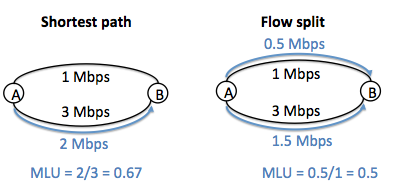
\includegraphics[scale=0.6]{fig/te-example.png}
	\caption{A flow-split routing reduces the maximum link utilization (MLU) over shortest-path routing.}
	\label{fig:te-example}
\end{figure}


If the traffic matrix is known accurately, the optimal solution to the traffic engineering problem can formulated as a multi-commodity flow optimization. The routing thus computed is refered to as \emph{optimal traffic engineering} in literature \cite{fortz2000internet,TEXCP}. As it is impossible to have accurate knowledge of future traffic matrices, traffic engineering schemes either take a \emph{demand-aware} or a \emph{demand-oblivious} approach. A demand-aware  traffic engineering  periodically updates routing using historically observed traffic matrices \cite{fortz2000internet,fortz2002traffic,COPE,MultiTM}. A demand-oblivious  traffic engineering  requires no explicit measurement of traffic matices, but instead configures routing statically. A common demand-oblivious technique is to use shortest path routing in which link weights are set to inverse of link capacities \cite{InvCap}, henceforth referred to as \invcap\ in this thesis. A demand-oblivious  traffic engineering is simple to implement because it does periodic traffic matrix measuremnt and routing configuration updates. 

%As it is impossible to have accurately knowledge of future traffic matrices. Therefore, practical traffic engineering schemes either take a demand-aware or a demand-oblivious approach.  A demand-aware  traffic engineering  periodically updates routing using historically observed traffic matrices. A demand-oblivious  traffic engineering  requires no explicit measurement of traffic matices, but instead configures routing statically. A demand-oblivious  traffic engineering  is simpler to implement because it requires neither measuremnt nor periodic updating of network routing. But, demand-aware schemes have been shown to outperform demand-oblivious  traffic engineering.

In practice, demand-aware traffic engineering based on Open Shortest Path First (OSPF) and Multiprotocol Label Switching (MPLS) are commonly used  \cite{COPE,MultiTM,fortz2000internet,MPLS2}. Routes computed by OSPF traffic engineering must follow shortest-weight paths, therefore OSPF TE provides limited functionality to split traffic among multiple paths. MPLS TE overcomes this limitation by enabling traffic between two nodes to be split  in arbitrary ratios among multiple paths. Therefore, MPLS TE gives better results than OSPF TE as exemplified above \cite{COPE,MultiTM}.

%Therefore, TE schemes commonly take a demand-aware approach, i.e., they compute routing using historically observed traffic matrices. In contrast, demand-oblivious simpler schemes also exist, no measurement of traffic matrix or continual updating of configuration. 

%But, future demand is not known perfectly. So, TE schemes commonly take a demand-aware approach: use historic demand patterns to predict future demand. In contrast, demand-oblivious simpler schemes also exist, no measurement of traffic matrix or continual updating of configuration. Demand-oblivious is simpler but demand-aware schemes have been shown to outperform them in TE literatue.

%
%Cost-based metrics: ignored the impact on end-user performance. So, what is the impact on end-user performance.
%
%TE is isolation, ignoring the internation with content placement and redirection.
%
%How do TE schemes compare when accounting for the interaction with content delivery.


\subsection{Content delivery}
\label{sec:ch2-cdn}

Content delivery systems seek to improve user-perceived performance for content accesses in all regions  at all times. A canonical example of a content delivery system is a content delivery network (CDN). State-of-the-art CDNs operate geo-distributed datacenters, and use a combination of edge caching, intelligent request redirection, and path and protocol optimizations for delivery of several types of content, e.g., video, bulk downloads, and interactive websites \cite{DilleyMPPSW02,akamai-overview}. Given their geo-distributed deployment, the decisions of content placement, i.e., locations at which acontent is placed, and request redirection, i.e., which location is best positioned to serve a user's request, are central to the functioning of a CDN.

\textbf{Content placement:} Content placement in CDNs is commonly done using caching schemes. For example a commonly used caching scheme is least recently used (LRU) cache replacement. There are two reason why content cahing is widely used. First, caching naturally captures geographic and temporal locality in content requests to populate caches with content likely to be reused. Second, a vast majority of network traffic is generated by content that gets updated infrequently, e.g., a video, audio, images. As a result, cached copies of content remain reusable for long duration. 

%Strong consistency is a separate topic and is studied in the content of design of geo-distrbuted kv store in auspice.\tbd{fix this}

\textbf{Request redirection:} In a CDN, request rediection occurs at two tiers - inter-datacenter and intra-datacenter. Our focus in this part of the thesis is on inter-datacenter request redirection because it influences wide-area traffic patterns that affect traffic engineering. We discuss intra datacenter redirection in the context of a content datcenter (Chapter \ref{ch:shrink}).

Request redirection strategies complement placement strategies by selecting the server location that is best suited to process a user's request. These strategies have been extensively studied and form the heart of CDN technology today. To quote from a report by Akamai,  \emph{``the system directs client requests to the nearest available server likely to have the requested content."} where the ``nearest" server is one whose round trip latency as well as packet losses are small, and  an ``available" server is one that has sufficient resources to serve a request \cite{DilleyMPPSW02}. 

Request redirection is implemented using three processes: (1) \emph{Monitoring:} Probe messages sent intermittently help monitor network characteristics and server load and identify congested regions of network and overloaded server locations \cite{oasis,donar}. (2) \emph{Estimating distances:} The measured statistics are combined to compute a distance function that reflects the proximity of a server location to users in a geographic region \cite{donar}. (3) \emph{Informing the user:} The user is informed of selected server/s either via DNS resolution \cite{DilleyMPPSW02} or via HTTP redirection \cite{barbir2003known}.

Content delivery techniques can be classified into demand-aware and demand-oblivious similar to our classfication of traffic engineering schemes. We consider common content delivery techniques discussed above to be demand-oblivious since they do not require long term content-level measurement of demand but instead use simple online heuristics to make their decision.. In contrast, a demand-aware approach to  placement and redirection has also been studied, e.g., Applegate \emph{et al.} \cite{ATTVoD} use a demand-aware approach to determine placement and redirection for Video-on-Demand content in the network. 

\subsection{Interaction between traffic engineering and application-layer adaptation}
\label{sec:ch2-te-cdn}

Studying the interaction between network-layer routing computed by traffic engineering and application-layer adaptation has been a topic of long standing interest in computer science. Several related questions have been put forth. Does this interaction yield globally sub-optimal results? How can we design cooperative mechanisms to leverage these interactions? Do cooperative mechanisms yield benefit in an Internet-like environment? Most previous research on this topic has focused on the interaction of traffic engineering with either overlay routing \cite{Roughgarden,selfishQiu} or with request redirection \cite{Jiang2009,JohariGameTheory, CATE, P4P} as discussed below. 

\textbf{Interaction between traffic engineering and overlay routing:} Several results show the negative interaction between selfish overlay routing and network routing \cite{Roughgarden,selfishQiu}. Theoretical results indicate that the negative interaction could cause an arbitrary degradation in user perceived delay. Further studies using Internet-like traffic demands and topologies indicate that this interaction hurts traffic engineering metrics. While this body of work focuses on application adaptation to \emph{path diversity} created by overlay routing, our work focuses on \emph{location diversity} present in the Internet (Chapter \ref{ch:beyondmlu}). We do not consider overlay routing since our focus is primarily on intra-domain routing while overlay routing is most commonly used to mask inter-domain routing inefficiencies \cite{Detour}. 


\textbf{Interaction between traffic engineering and request redirection:} Recent work has studied the interaction between ISP traffic engineering and request redirection by content providers with geo-distribtued datacenters as well as P2P applications. Both analytical results \cite{Jiang2009,JohariGameTheory} and system implementations \cite{CATE,P4P} have shown that there is value for joint optimization of request redirection and traffic engineering, and cooperative strategies can help traffic engineering metrics while maintaining or improving user-perceived performance. Our work distinguishes in that  we model the three-way interaction between placement, redirection and routing and show that placement flexibility is more powerful degree of freedom than redirection or routing to improve traffic engineering metrics and to reduce user-perceived latency (Chapter \ref{ch:ncdn}).


\section{Motivation}
\label{sec:bg-motivation}

A content-dominated traffic and the presence of content at multiple network locations changes the traditional ISP traffic enginering problem. In such a network, a traffic matrix is no longer an effective representation of demand. It can be changed via application-layer adaptation without any underlying change in demand. Demand is better expressed as a \emph{content matrix} in which each entry represents the demand for a content at a particular network location. A traffic matrix implicitly assumes a fixed source and a fixed destination for each traffic flow. But, a content matrix expresses the fact that the demand for a content at a particular destination can be served from any set of source locations. As we explain using examples below, the flexibility of serving the demand from any location raises questions on the usefulness of link-utilization based metrics that are commonly used in traffic engineering (Section \ref{sec:bg-poormlu}) as well on the importance of traffic engineering itself (Example \ref{sec:bg-ncdn-interaction}). These and other related questions motivate our work on traffic-engineering in content-dominated networks.

Our work presents research on two network scenarios that vary in terms of application adaptation mechanism and the content placement flexibility in the network. We explain the two scenarios and motivate the research questions we address in each case using examples.

\subsection{ISP network with content location diversity}
\label{sec:bg-locdiv}
We consider an ISP network that has little control over placement and redirection, but applications can leverage \emph{location diversity}, or  the ability to download content from multiple locatioons. We motivate why traffic engineering schemes must be evaluated while accounting for their interaction with location diversity, and why we need to look beyond link-utilization based metrics in evaluating traffic engineering schemes. These questions are addressed in Chapter \ref{ch:beyondmlu}.

\subsubsection{Interaction between traffic engineering and location diversity}
\label{sec:bg-3node}

\begin{figure}[tbh]
	\centering
	\label{fig:3node-bg}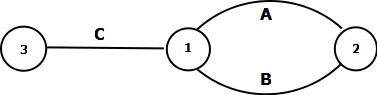
\includegraphics[scale=0.5]{final_images/Diagram3node.png}
	\caption{Lasso network}
\end{figure}

This example illustrates how location diversity can change the traffic matrix without any underlying change in demand. In Figure~\ref{fig:3node-bg}, all links are assumed to have a capacity of 100 units and a constant delay. The top link A has a very small delay compared to the other two links that both have equal delay. Node 1 has 100 Mbps of demand that it can obtain from 2 as well as 3. In addition, there is 20 Mbps of demand at node 1 which it can obtain only from 2.  We assume that the aggregate demand at a node consists of a large number of user-initiated connections. When content can be downloaded from multiple locations, users initiate parallel TCP connections and the throughputs along paths in a parallel TCP connection are inversely proportional to the path delays. The TE scheme is assumed to be OSPF-based, i.e., shortest-path routing using configured link weights and traffic split equally among multiple paths with equal weights.

Suppose the weights of the links A and B are unequal and the link A has more weight. As a result, all of the traffic between 1 and 2 is routed using only link B. 1 splits its demand of 100 Mbps using parallel TCP equally between links B and C. Thus, the traffic on links A, B, and C is  0, 70, and 50 respectively. In the next step, seeking to balance load better for this resultant matrix, the TE scheme sets both the links A and B to the same weight (hoping to achieve link utilizations of 35, 35, and 50 respectively).  Consider how parallel TCP connections respond to this change. Assuming each TCP connection between 1--2 is pinned to only one of the two paths---as is commonly done in practice to achieve equal-cost multi-path (ECMP) splitting---50 Mbps of demand at 1 gets routed using parallel TCP connections over the link A and link C, and an equal amount using parallel TCP connections along the link B and link C. In addition, the 20 Mbps of background traffic is split equally among link A and link B as per ECMP.  Since link A has a much smaller delay than link C, the 50 Mbps of demand at 1 using parallel TCP along those two paths will flow entirely through link A. The remaining 50 Mbps using B and link C will get split equally across the two paths by parallel TCP. Thus, the traffic on the links A, B and C is 60, 35, and 25 respectively, which is different from what the TE scheme engineered for (namely, 35, 35, and 50). The resulting MLU of 0.6 is different compared to 0.5, the value that the TE scheme expected. This example illustrates that the outcome of traffic engineering depends on the application adaptation to location diversity, thereby motivating us to study the following question.

\emph{Research question: How do traffic engineering schemes compare while accounting for the effect of location diversity in the network?}

\subsubsection{Shortcomings of link-utilization metrics}
\label{sec:bg-poormlu}

%We explain why link-utilization based metrics may not reflect user-perceived performance. Further, they are a poor metric to measure network capacity, i.e., the factor of surges in traffic demand that a network can tolerate, in a network with location diversity.

Link-utilization based metrics may not be a good predictor of user-perceived performance that depends on other factors such as propagtion delay, access link capacity and backbone link capacity also. Moreover, queuing-theoretic models show that only a high link utilization severely affects performance-critical metrics such as queuing delay and packet loss \cite{mm1}. For low to moderate link utilization that is common in today's ISPs, a reduction in link utilization may not yield a commensurate benefit in application peformance. 

\emph{Research question: Are link-utilization based metrics good predictors of user-perceived performance for real network topologies and traffic matrices?}

Link-utilization based metrics, in particular inverse of MLU, are a poor capacity metric in the presence of location diversity. In using inverse of MLU as a capacity, we implicitly assume that traffic matrices scale linearly as network traffic increases. 
But, this assumption may not hold if in a network where application adaptation to location diversity determines the traffic matrix as in the above example. Thus, location diversity necessitates a new capacity metric.

\emph{Research question: How do we quantify network capacity under location diversity?}

\subsection{Network CDN}
\label{sec:bg-ncdn}
Network CDNs are a recent, potentialy transformative trend in which ISPs deploy CDNs on their infrastructures to deliver content to users on their network.  Unlike traditional ISPs and traditional CDNs, NCDNs enjoy full control over placement, redirection and routing on their networks. The interaction between placement and routing in an NCDN illustrated below motivates us to explore the benefit of joint optimization of placement, redirection and routing as well as to evaluate the relative importance of placement and routing in an NCDN. These questions are addressed in Chapter \ref{ch:ncdn}.

\subsubsection{Interaction between placement and routing in an NCDN}
\label{sec:bg-ncdn-interaction}

To appreciate how placement can shape traffic in an NCDN, consider the simple example in Figure~\ref{fig:NetworkExample}. Node $C$ has an object in its cache that is requested by end-users at nodes $A$ and $D$. Suppose that one unit of traffic needs to be routed from $C$ to $A$ and $0.5$ units  from $C$ to $D$ to satisfy the demand for that object. The routing that achieves the minimum MLU of $0.5$ to serve the demanded object is shown in the figure. Note that the routing that achieves the MLU of 0.5 is not possible with a simple, \unplanned\ scheme like \invcap\ as that would route all the traffic demand from $C$ to $A$ via $B$, resulting in an MLU of 1. Thus, a (\planned) traffic engineering scheme is necessary to achieve an MLU of 0.5.

\begin{figure}[h]
	\centering
	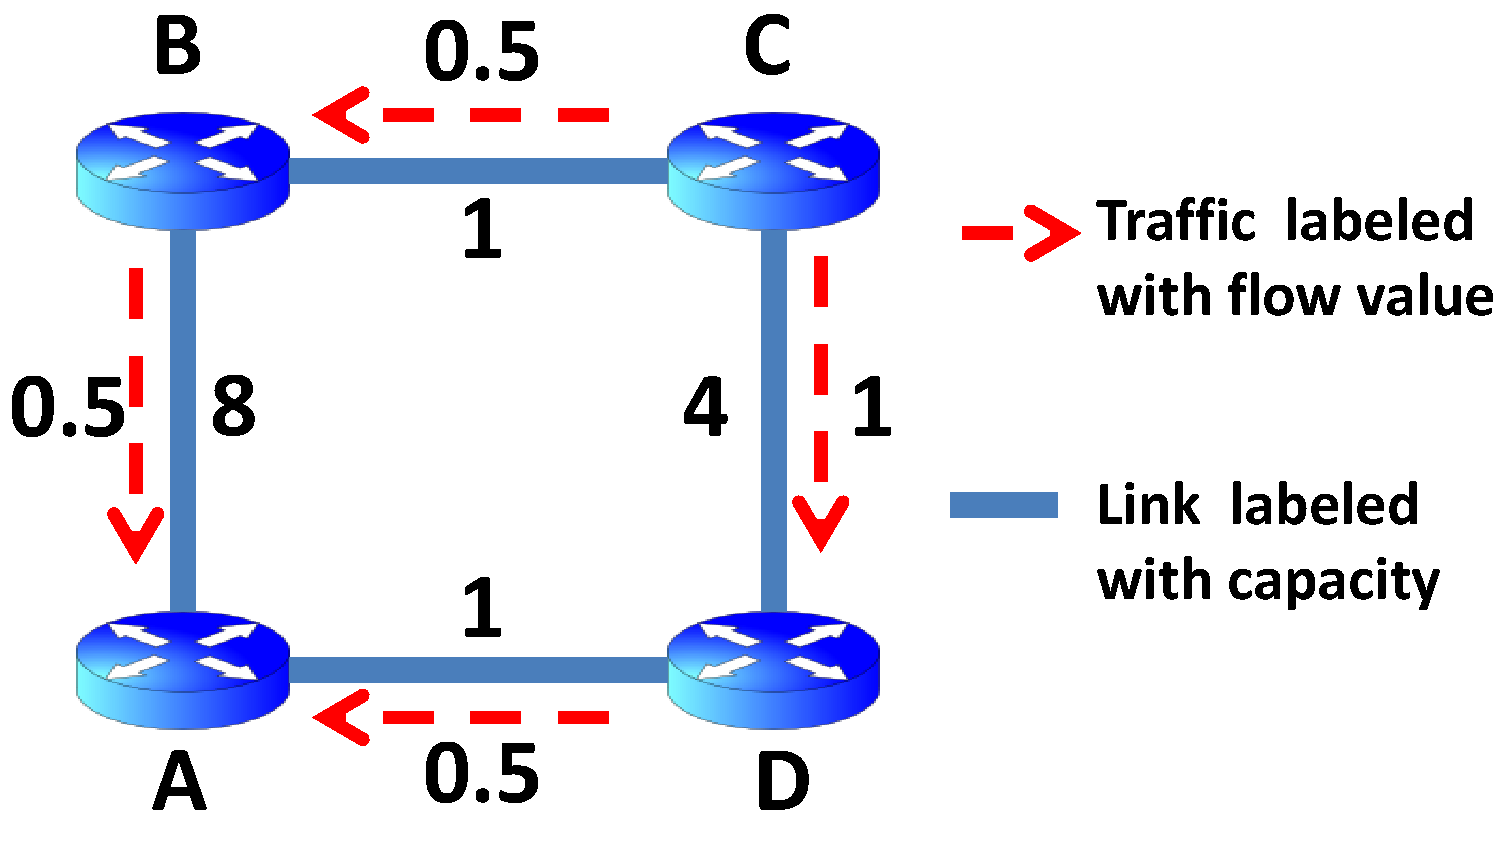
\includegraphics[width=2in]{ncdnpaper/ncdn-example}
	\caption{A simple \ncp\ example}
	\vspace{-.3in}
	\label{fig:NetworkExample}
\end{figure}

On the other hand, NCDNs can shape the traffic demand matrix by using a judicious placement and redirection scheme. Suppose that there is some space left in the content server's cache at node $B$ to accommodate an additional copy of the demanded object. By creating an additional copy of the object at $B$, the traffic demand of $A$ can be satisfied from $B$ and the demand of $D$ from $C$ achieving an MLU of $0.125$. In this case, judicious content placement decreased the MLU by a factor of $4$. Even more interestingly, this best MLU can be achieved using a simple routing scheme like \invcap\ routing while also improving user-perceived latency (assuming that the latency of link $BA$ is lower than that of the two-hop paths from $C$ to $A$). While this is a toy example, it shows that content placement flexibility reduces network cost and enables simpler routing. This interaction between placement and routing motivates us address the following questions for real content workloads and network topologies. 

\emph{Research question: Does a joint optimization of placement, redirection and routing yield benefits over independently making these decisions using simple demand-oblivious schemes in an NCDN?}

\emph{Research question: Does content placement flexibility obviate sophisticated traffic engineering in an NCDN?}




%A Network CDN (NCDN) is an ISP than owns and operates a CDN over its infrastructures to deliver content to its end users. As NCDNs manage both the underlying network and content delivey, the objectives and the techniques available to a network CDNs are not the same from a traditional ISP or a tradidional CDN. Our work is motivated by the following questions:
%
%\begin{itemize}
%	\item 
%	Is a demand-aware or a demand-oblivious content delivery and traffic engineering scheme more effective for a network CDN?
%	\item
%	An NCDN can potentially jointly optimize content delivery and traffic engineeing, but do such sophisticated schemes yield benefits from a CDN?
%\end{itemize}
%
%To our knowledge, this thesis presents the first study of techniques for a managing a NCDN based on real network topology and content access traces. Our result show the effectiveness of simple demand-oblivious schemes for content delivery and traffic engineering in achieving performance close to an ideal scheme. Further, they show that a demand-aware joint optimization performs poorly due to frequnt churn in content workloads and change in access patterns. 






%%!TEX root = New.tex
\chapter{Background}
\label{ch:background}
\eat{
\begin{itemize}
\item
More than a literature review
\item
Organize related work - impose structure
\item
Be clear as to how previous work being described relates to your own.
\item
The reader should not be left wondering why you've described something!!
\item
Critique the existing work - Where is it strong where is it weak? What are the unreasonable/undesirable assumptions?
\item
Identify opportunities for more research (i.e., your thesis) Are there unaddressed, or more important related topics?
\item
After reading this chapter, one should understand the motivation for and importance of your thesis
\item
You should clearly and precisely define all of the key concepts dealt with in the rest of the thesis, and teach the reader what s/he needs to know to understand the rest of the thesis.
\end{itemize}
}

This thesis builds on prior research in three areas: traffic engineering, content delivery, and the interaction of the two. We first review the major classes of traffic engineering strategies (Section \ref{sec:bg-te}). Next, we discuss common techniques used by content delivery systems, including strategies for content placement and for request  redirection (Section \ref{sec:bg-cdn}). Finally, we survey research on the interaction between network and content delivery, and find that the interaction between traffic engineering and either overlay routing or request redirection have been the focus of past research (Section \ref{sec:bg-interaction}).



\section{Traffic engineering}
\label{sec:bg-te}

The goal of traffic engineering (TE)  is to avoid congestion hotspots in the network by optimizing routes based on network topology and expected traffic demand. In the context of large Internet service provider (ISP) networks, traffic engineering decides both intra-domain (within the ISP) and inter-domain routing (across ISPs). We focus here on intra-domain routing and refer the reader to  \cite{Feamster2003,rexford} for a survey of inter-domain traffic engineering. 





We classify traffic engineering schemes based on the frequency at which they update routing. By this attribute, TE schemes can be grouped into three categories: (1) \emph{Demand-oblivious TE} uses static routes that are seldom updated \cite{Cohen,Racke}. (2) \emph{Demand-aware TE}  updates routes periodically, e.g., every few hours or every few days, based on recent history of traffic demand \cite{fortz2000internet,fortz2002traffic}. (3) \emph{Online TE} updates routes at timescales of hundreds of milliseconds, reacting instantaneously to traffic demand changes \cite{TEXCP}.

TE schemes are evaluated based on link utilization based metrics, e.g., a widely used metric is maximum link utilization \cite{COPE}. A TE scheme is usually compared against the optimal solution that minimizes the given metric by solving a multi-commodity flow optimization  \cite{TEXCP,fortz2000internet}.
By this measure, oblivious routing schemes perform poorly and can be shown to be arbitrarily worse compared to the optimal strategy  \cite{fortz2000internet}. For many ISPs networks, simple oblivious routing schemes are sub-optimal by a small constant factor  \cite{COPE,MultiTM,TEXCP}.
Offline TE schemes, while sub-optimal, perform superior to oblivious TE schemes. e.g., Fortz and Thorup show that   offline TE delivers up to 2$\times$ better on AT\&T network backbone. Online schemes have been shown to achieve near-optimal performance, but they are rarely used in production networks.

In practice, offline TE based on Open Shortest Path First (OSPF) and Multiprotocol Label Switching (MPLS) are commonly used  \cite{COPE,MultiTM,fortz2000internet,MPLS2}. Routes computed by OSPF traffic engineering must follow shortest-weight paths, therefore OSPF TE provides limited functionality to split traffic among multiple paths. 
MPLS TE overcomes this limitation by enabling traffic between two nodes to be split  in arbitrary ratios among multiple paths.
Therefore, MPLS TE gives better results than OSPF TE  \cite{COPE,MultiTM}.



Prior work on traffic engineering is based primarily on evaluation of link utilization based metrics, and has largely ignored the impact of traffic engineering on user-perceived performance. Further, the comparison of TE schemes has not taken into account the interaction with content delivery. This thesis contributes in answering these questions. In Chapter \ref{ch:beyondmlu}, we provide a comparison of traffic engineering schemes focusing on user-perceived metrics such as file download times, and VoIP call quality. In Chapter \ref{ch:beyondmlu} and Chapter \ref{ch:ncdn}, we evaluate TE schemes while accounting for the interaction between TE and content delivery and show that this interaction helps simpler TE schemes, such as oblivious TE or OSPF TE, perform closer to the optimal TE strategy in terms of user-perceived metrics as well as TE metrics.

%Server shutdown policies that concentrate traffic on the smallest possible subset of network topology indeed enable maximum network energy savings. 

%In Chapter 5, we show that server shutdown policies that concentrate traffic on the smallest possible subset of network topology indeed enable maximum network energy savings. 



%Network energy savings due to energy-aware traffic engineering depends on traffic patterns in the network, traffic patterns that are assumed to be fixed. In the case of CDN data centers, traffic patterns could be shaped by load balancing decisions and server shutdown policies. In Chapter 5, we investigate TE strategies that coordinate with datacenter load balancing decisions and server shutdown policies, and yield greater network energy savings than shown by prior work.

%We hypothesize that  there exists potential for more network energy savings in datacenters than shown previously, provided techniques for saving server energy work in coordination with those for saving network energy. 

%\textcolor{red}{How much energy could be further saved in scenarios where content placement flexibility exists?}

%The above discussion has focused more on traffic engineering in wide-area networks. Traffic engineering in data center networks is another very active research area and we refer the reader to  \cite{,,} for few recent papers.

%In comparison to approaches that optimize routing for a given traffic matrix, this paper shows that a joint optimization of content placement and routing for content-serving clusters yields greater network energy savings.

\section{Content delivery}
\label{sec:bg-cdn}
Content delivery systems seek to provide a high-quality experience to users accessing content in all regions  at all times. A canonical example of a content delivery system is a content delivery network (CDN). State-of-the-art CDNs operate geo-distributed datacenters, and use a combination of edge caching, intelligent server selection, and path and protocol optimizations for delivery of several types of content, e.g., video, bulk downloads, and interactive websites \cite{DilleyMPPSW02,akamai-overview}. Given their geo-distributed deployment, the decisions of content placement, i.e., locations at which a content is placed, and request redirection, i.e., which location is best positioned to serve a user's request, are central to the functioning of a CDN.

%The design of a content delivery system must consider the unpredictable nature of the Internet and of content workloads. The unpredictability arises from changes in network conditions, sudden spikes in content popularity, as well as malicious traffic generated by DDoS attacks. To provide quick response to these events, content delivery systems must use algorithms that are computationally efficient. Content delivery systems of today use distributed heuristics, often trading optimality for efficiency, to ensure high-quality user experience in all regions at all times.

\subsection{Content placement}
\label{sec:placement}
Placement strategies depend on whether content is static or dynamic. 
Dynamic content has limited cacheability therefore placement  strategies for static content are not always applicable for dynamic content.

\subsubsection{Static content placement}
\label{sec:static}
Static content, such as videos, audio, images and software updates, contribute to a vast majority of traffic in the Internet \cite{nielsen-video-growth,cisco-videogrowth}.  The placement of static content is commonly handled by a caching strategy. A simple and widely used caching strategy is least recently used (LRU) cache replacement  \cite{wessels2009squid}. Caching strategies are effective because they exploit geographic and temporal locality of requests, resulting in high cache hit rates in many cases  \cite{davison2001web,NCDN,gadde2001web}. 
An alternative to caching is a planned placement approach,  which prepositions content at a set of locations based on prior knowledge of demand. Planned placement is effective in scenarios where workloads are predictable over long intervals, e.g., hours, or days \cite{Applegate2010}. 



%Little attention that these placement strategies have on networks.

\subsubsection{Dynamic content placement}
\label{sec:dynamic}
Several applications today generate dynamic content such as stock prices, weather information, price catalogs. Such dynamic content is typically stored at a small number of fixed locations across the globe, mostly for fault tolerance objectives  \cite{sql-geo-replication}. Due to a limited number of fixed replica locations,  content accesses from regions away from the replica locations incurs high latency \cite{sql-geo-replication,volley}. Extensively replicating dynamic content is costly due to bandwidth and server resources used in propagating updates to  all locations. 

Placement strategies for dynamic content is an active research area. A naive placement strategy of replicating all data at all locations would incur high update costs. The alternatives provided by current systems either require manual configuration to decide placement or result in sub-optimal latency.
For example, Spanner  \cite{spanner} provides configuration options to manually select which locations should a given subset of data be replicated. 
DHT-based systems automatically decide placement but result in high latency because replica are chosen randomly \cite{beehive,codons-paper}.
Volley  \cite{volley} uses a placement heuristic to select a single best location for each data item, but it would result in sub-optimal latencies when a data item is popular across many geographic regions.

This thesis addresses the problem of dynamic data placement across geo-distributed data centers while enhancing prior work in this area (Chapter \ref{ch:auspice}). Our system, Auspice, automatically makes data placement decisions (unlike Spanner), places data replicas based on demand-locality (unlike DHT-based replication), and creates multiple replicas of each object (unlike Volley) �and limits update propagation costs.

\subsection{Request redirection}
\label{sec:redirection}

Request redirection strategies complement placement strategies by selecting the server location that is best suited to process a user's request. These strategies have been extensively studied and form the heart of CDN technology today. To quote from a report by Akamai,  \emph{``the system directs client requests to the nearest available server likely to have the requested content."} where the ``nearest" server is one whose round trip latency as well as packet losses are small, and  an ``available" server is one that is lightly loaded considering all resources, i.e., network, CPU and disk  \cite{DilleyMPPSW02}. 

Request redirection is implemented using three processes: (1) \emph{Monitoring:} Probe messages sent intermittently help monitor network characteristics and server load and identify congested regions of network and overloaded server locations \cite{oasis,donar}. (2) \emph{Estimating distances:} The measured statistics are combined to compute a distance function that reflects the proximity of a server location to users in a geographic region \cite{donar}. (3) \emph{Informing the user:} The user is informed of selected server/s either via DNS resolution or via HTTP redirection as described in  \cite{DilleyMPPSW02} and  \cite{barbir2003known}.




% Analysis of traces within a data center has shown that servers are typically lightly loaded. 
% Motivated by this observation, several papers  \cite{mathew12,Jain,lin12,lu13}, based on trace-driven experiments,  have explored how much energy savings can be obtained by using only a fraction of the servers at a given time, and by shutting-off remaining servers or switching them to a low power state.
 


\section{Interaction between network and content delivery}
\label{sec:bg-interaction}

Studying the interaction between network and content delivery has been a topic of much interest in both systems and theory communities. Several related questions have been put forth. Do these interactions negatively affect objectives of networks and content delivery systems? What is the sub-optimality caused due to these interactions in the worst case, and for typical topologies and traffic demands? How to leverage these interactions to improve traffic engineering and content delivery objectives? 

Yet, we don't fully understand these interactions because prior research has studied the interaction of network routing with only a subset of content delivery decisions. 
Much prior research has focused on two aspects: the interaction of overlay routing and network routing  \cite{Roughgarden,selfishQiu}, and the interaction of request redirection and network routing  \cite{Jiang2009,JohariGameTheory, CATE, P4P}. While placement decisions are critical to user-perceived performance, there has been little research on how content placement interacts with network routing.

\subsection{Interaction between traffic engineering and overlay routing}
\label{sec:overlayunderlay}

Several results show the negative interaction between selfish overlay routing and network routing \cite{Roughgarden,selfishQiu}, however it appears that selfish overlay routing is not used by most of the Internet traffic. 
%Theoretical results indicate that the negative interaction could cause an arbitrary degradation in user perceived delay. Further studies using synthetic traffic demands and topologies indicate that this interaction hurt traffic engineering metrics.  
%However, it appears that a small fraction of Internet traffic uses overlay routing. 
For example, traffic from CDN edge server to the client always follows network routing. Further, overlay routing yields ``marginal" benefits ($<$ 30\%) over network routing for 79\%-96\% of paths depending on which geographic region is being considered  \cite{rahul2006overlays}, which suggests that traffic between CDN servers forming an overlay network follows network routing in most cases. For this reason, this thesis does not model the interaction between overlay and network routing.


%Despite several results regarding negative interaction of seflish overlay routing and network routing, its implications for present day Internet are not clear. Theoretical results indicate that the negative interaction could cause an arbitrary degradation in user perceived performance. Further studies using synthetic traffic demands and topologies indicate that this interaction could hurt the performance of traffic engineering schemes.  However, in today's Internet, it is not clear what fraction of traffic follows overlay routing. For example, traffic from CDN edge node to the client always follows network routing. Further, overlay routing yields "marginal" benefits (< 30%) over network routing for 79%-96% of paths depending on which geographic region is being considered. Therefore, in this thesis, we assume that all traffic is compliant to network-routing. 
%
%Traffic from CDN edge node to the client, which form a bulk of traffic always follows network routing. Similarly, traffic between overlay nodes 
%
%
%
%
%In the worst case, the negative interaction could cause an arbitrary degradation in user perceived performance; for typical networks and traffic demands, performance degradation is a small factor.
%
%
%Subject: prior studies ignore a key component of this interaction, which is the role of placement strategies. 
%
%prior work 1: overlay vs network routing
%
%results: negative effect on traffic engineering, close to optimal delay in internet-like environments. In this thesis, assuming that all traffic is network-routing compliant. 
%
%we do not consider the interaction of overlay vs network routing.
%
%prior work 2: redirection vs network routing
%
%Commonly, these efforts assume that all content is available at all locations, ignoring the fact that that content availability at a location depend on placement strategies. Therefore, placement strategies must be taken into account in studying this interaction.
%
% 
%
%Interaction between overlay routing and underlay routing does happen, but it happens only for a small fraction of traffic. Traffic from CDN edge node to the client, which form a bulk of traffic always follows network routing. Similarly, traffic between overlay nodes 
%
%While placement decisions are critical to user-perceived performance, little research in this area has focused how they interact with traffic engineering.
%


% Therefore, as a simplification, we assume that all traffic is compliant to network-routing. 


%While theoretical results indicate that the negative interaction could cause an arbitrary degradation in user perceived performance. In the worst case, the negative interaction could cause an arbitrary degradation in user perceived performance; for typical networks and traffic demands, performance degradation is a small factor.While traffic engineering selects a set of physical links to route traffic, overlay routing selects a path consisting of a sequence of intermediate  overlay nodes on way to the destination.  Overlay routing negatively interacts with traffic engineering if all flows are  allowed to selfishly choose overlay routes. In the worst case, the negative interaction could cause an arbitrary degradation in user perceived performance; for typical networks and traffic demands, performance degradation is a small factor. However, a network layer routing that is very inefficient could benefit from an overlay routing, if overlay routes in a coordinated fashion. Therefore, negative interactions between overlay routing and traffic engineering happen, but not always.


\subsection{Interaction between traffic engineering and request redirection}
\label{sec:jointopt}

Recent research has investigated the interaction between request redirection and traffic engineering, without considering the role of placement strategies. This interaction is commonly studied in the context of Internet service providers (ISPs) and content providers (CPs) with geo-distributed datacenters. 
Both analytical results \cite{Jiang2009,JohariGameTheory} and system implementations \cite{CATE,P4P} have shown that there is value for joint optimization of request redirection and traffic engineering, and cooperative strategies can help traffic engineering metrics and also reduce user-perceived latencies. Commonly, these efforts assume that all content is available at all locations, ignoring the fact that content availability at a location depend on placement strategies. Therefore, in this thesis, we account for the effect of content placement along with request redirection, in studying the interaction between network and content delivery.

\section{Summary}
\label{sec:summary}
In this chapter, we reviewed prior research on traffic engineering and summarized different classes of traffic engineering schemes. We also reviewed common techniques used for content delivery, namely strategies for placement of static content and of dynamic content, and request redirection techniques used by CDNs. Finally, we reviewed research on interaction between network and content delivery, and found that much prior research in this area has focused on two aspects, the interaction of overlay routing and network routing, and the interaction of request redirection and network routing.

\eat{Our survey of work in traffic engineering, content delivery and interactions between them has shown the following directions for research, which we pursue in this thesis: (1) how does content placement strategy shape the interaction between network and content delivery, and how it affects the performance and cost metrics of networks and content delivery systems? (2) how do we design a system for placing dynamic objects across geo-distributed data centers, while minimizing request latencies, limiting resource cost of update propagation, and providing desired consistency guarantees?}


\eat{
Traffic engineering is the process by which network operators select routes for avoid congestion hotspots in the network. We can categorize TE schemes into oblivious, offline, and online. Commonly, offline TE schemes using either OSPF or MPLS are widely used in ISP networks.

Content delivery depends on two key decisions of content placement and request redirection. Placement for static content is done by CDNs using cache replacement policies such as least recently used (LRU). Placement of dynamic content is done via fixed placement policies, such as k-random, which results in a sub-optimal latency. Request redirection strategies complement placement strategies in optimizing user-perceived performance by directing a user to the best positioned server based on network latency, path loss rates, and load on the server. Redirection strategies have been studied extensively and are widely used by CDNs today.

The interaction between network and content delivery has been studied both in systems and in theory research communities. Much prior research in this area has focused on two aspects, the interaction of overlay routing and network routing, and the interaction of request redirection and network routing. A key open question, that we address in this thesis, is how does the placement of content shape the interaction between network and content delivery, and how it affects the performance and cost metrics of networks and content delivery systems.

}

%%!TEX root = shrink.tex

\section{Discussion}
\label{sec:discussion}

\textbf{Energy use vs. energy cost:} There are three types of \cdc s in terms of their energy cost to an operator. 

\emph{(1) Operator-owned facility:} If a \cdc\ operator owns the datacenter facility, it directly pays to the electricity companies based on its usage. In such datacenters, a reduction in energy use by \shrink\ is likely to bring a reduction in electricity costs as well.

\emph{(2) Co-location facility:} A \cdc\ at a co-location facility typically pays by the provisioned power and not the electricity used \cite{qureshi2009cutting}. Therefore, a reduction in energy use will not bring cost savings to \cdc\ operator with the existing pricing models. However, it is possible a \cdc\ operator may use the reduced energy as a leverage for negotiating a cheaper pricing. 

\emph{(3) Co-location inside ISP networks:} A \cdc\ at a co-location facility maintained by an ISP often has a symbiotic relation with the ISP, where the \cdc\ caches content to reduce the inter-domain traffic for the ISP while an ISP provides co-location free of charge \cite{google-caching}. In such \cdc s, energy savings do not translate to cost savings to the \cdc\ operator.  Although, energy savings do benefit the ISP, who eventually pays for the electricity.

The type of usage-based energy pricing also determines the cost savings for an operator. Specifically, we distinguish between flat rate pricing and time-of-use pricing \cite{pge-website}. With a flat rate pricing, a given percentage reduction in the energy use results in the same percentage reduction in the energy cost. With a time-of-use pricing, the percentage reduction in the energy use and the energy cost may not be the same. For example, if the peak load on a \cdc\ coincides with the peak hour of electricity prices, the percentage reduction in the energy cost would be lower than the percentage reduction in the energy use.

%\textbf{\shrink\ as a dynamic provisioning tool:} \shrink\ can be used as a dynamic provisioning tool by an operator that is running a content delivery site on infrastructure rented from a cloud-computing platform such as Amazon EC2. In such a setting, the operator may use \shrink\ to dynamically provision the number of active servers in accordance with incoming request load. In such a setting, the operator may not be able to perform network consolidation, but it can run the server energy optimization and load balancing sub-systems of \shrink\ and dynamically provision the number of active servers in accordance with incoming request load.  While functioning as a dynamic provisioning tool, \shrink\ can help reduce infrastructure costs for the operator.

\textbf{Impact on web-page load time:} Our prototype-based experiments evaluate the response time for individual HTTP requests, and hence do not capture a key metric that is more relevant from an end-user's perspective: web-page load time. However, we expect the inflation in web-page load time to be lower than the inflation in response times given that computation in web browsers constitutes up to 35\% of the critical path of a web-page load time \cite{wprof}.



\section{Related work}

Our effort distinguishes from prior work in quantifying the energy-response time tradeoff  in \cdc s, presenting the design and implementation of a system to leverage this tradeoff and proposing a network-aware server consolidation scheme to reduce network energy use.  Prior work on reducing energy of datacenters can be divided into three topics: (1) power-proportionality of servers and switches.  (2) server and network consolidation in a datacenter and (3) global load balancing across datacenters.

\textbf{Power-proportional servers and switches:}  Several efforts have focused on reducing energy use of a server's sub-systems such as CPU \cite{dvfs}, disk \cite{lu1999adaptive}, and memory \cite{fan2001memory}. Similarly, Nedevschi et al. \cite{Nedevschi08} study power management for switches that support sleep states or several power/performance states similar to CPUs. Nonetheless, today's servers and switches are far from power-proportional. Mahadevan et al. show that networking equipment consumes 62\%-91\% of their peak energy in idle state \cite{mahadevan2009power} and servers consume 32\% to 42\% of maximum power at a small utilization of 10\% \cite{spec}. Until the ideal of power-proportionality is achieved, consolidation remains a promising approach to save energy.

\textbf{Server consolidation:} Given the long line of work in server consolidation, our work does not focus on saving more energy than the existing consolidation schemes, but instead on accurately quantifying the impact on response times of a simple consolidation scheme.
%Both analytical and experimental studies of server consolidation have been previously explored. 

%A long line of work has studied consolidation techniques to reduce datacenter energy, including efforts that are analytical in nature as well as implementation-based efforts. 

The analytical work in this area shares similar goals as us.  Lin et al. \cite{lin12} propose an algorithm for optimizing a cost metric that incorporates energy costs, on-off switching costs and cost of degradation in performance. Mathew et al. \cite{mathew12} propose an algorithm that balances energy use, reliability and availability of servers, which they evaluate based on load traces from Akamai datacenters. In comparison, our implementation-based approach enables us to accurately model the relation between server utilization and response time, impact of server consolidation on cache hit rates, and non-ideal load balancing, to accurately quantify the impact of consolidation on response time for \cdc s.

Several efforts have conducted an implementation-based evaluation of server consolidation for stateless systems. Chase et al. \cite{chase2001managing} allocate resources among multiple co-hosted services in a cluster while reducing energy via consolidation. Pinheiro's \cite{pinheiro2001load} system proposes consolidation and load balancing algorithms given a bound on the performance degradation that is acceptable.  Rajamani et al. \cite{rajamani2003evaluating} evaluate consolidation schemes for a modified TPC-W workload. In comparison, our effort focuses on \cdc s that maintain a large amount of state in the form of cached content. In \cdc s, the effect of consolidation on response times cannot be evaluated accurately without accounting for the effect of consolidation on the availability of cached content and the resulting cache hit rates.
%One of our key findings is that consolidation results in a small impact on cache hit rates, which helps \shrink\ achieve a good energy-response time tradeoff.

Trushkowsky et al. \cite{Trushkowsky:2011}  dynamically allocate servers and reconfigure the data stored on the servers to meet service-level objectives such as 99-th percentile request latency.  However, there are two key differences between their work and ours. First, they focus  on a workload exclusively of small (256B) objects stored in-memory, whereas  \cdc s need to deal with orders of magnitude of heterogeneity in object sizes and extensively use a disk cache to improve hit rates.  Second, their system appears to be a backend data store, which always has content available within the datacenter. In comparison, \cdc s have a significant fraction of traffic to remote datacenters due to cache misses, and the impact of consolidation on response time in \cdc s depends on the increase in traffic to remote datacenters that consolidation causes. For these reasons, it is not clear if their findings on the impact of dynamic server allocation on request latency would be applicable for \cdc s.
%One of our key findings is that consolidation results in a small increase in cache miss rates, which helps \shrink\ achieve a good energy-response time tradeoff. 

%\TBD{we optimize network energy use also}

\textbf{Network consolidation:} Network  consolidation has been studied for both wide-area and data center networks \cite{response, elasticTree, greenTE, Chiaraviglio, Andrews}. Network consolidation concentrates traffic, represented in the form of a traffic matrix, on a subset of links and switches, and turns off remaining switches and links to save energy. Our work differentiates from prior work in two ways. First, prior work evaluates schemes mostly using traffic engineering metrics such as link utilization, while we evaluate actual end user response time for a real application and show that network consolidation can be performed with a small performance impact in \cdc s. Second, we show network consolidation is closely related to server consolidation. Our network-aware server consolidation saves up to 45\% more network energy over a network-unaware server consolidation scheme.
%network-aware server consolidation increase the potential savings that a network consolidation scheme can achieve. 
%
%
%
%
%
%
% with little effort on measuring response times for real applications
%
%While previous work has studied server and network consolidation as independent problems, we show that these problems are closely related. For the same number of servers, which set of servers is chosen affects potential energy savings that a network consolidation scheme can achieve. Further, we propose a simple network-aware server consolidation scheme saves up to 45\% more network energy over a network-unaware server consolidation scheme.

\textbf{Global load balancing:} Many papers \cite{Liu11,qureshi2009cutting,Gao12,Rao10}  have shown that geographical load-balancing across data centers can exploit the differences in electricity prices and in renewable energy availability at various locations to reduce energy costs, energy use, or non-renewable energy use.  In comparison, our work focus on improving energy-efficiency of a single \cdc\ by the use of consolidation. We believe that global load balancing can complement \shrink\ in reducing energy use and its cost across datacenters.


% new chapter
%%!TEX root = ../New.tex
\chapter{Resource management on a  geo-distributed platform}

\section{Goals}

The goal is to design a platform that makes it easy to deploy applications on a global scale. The system runs on a geo-distributed platform spanning up to thousands of locations worldwide and runs up to thousands of applications on this platform. This global platform manages both compute and storage resources for every application across geo-distributed data centers.  

An application divided into two logical tiers: a storage tier  and a processing tier. Each application has an SLA specified in terms of 95-percentile request latencies and a minimum number of deployment locations for fault tolerance. 


\begin{itemize}
\item
Which locations should each application be deployed given the storage and server constraints at a location and the geo-distribution of demand patterns?
\item
How to dynamically allocate server/storage resources for an application at a location?
\item
Whether to add/remove the set of deployed locations for an application based on the current load?
\item
How to allocate/deallocate resources across data centers dynamically?
\item
At what timescales should these decisions be made?
\item
How to reduce operational costs while meeting SLAs of various applications?
\item
How to ensure fairness across applications? And how to balance fairness and the goal of maximizing aggregate utility of the system?
\end{itemize}


In the simplest case, if all applications are uni-dimensional and our objective is to minimize user-perceived latency for a static workloads, then the formulation presented in Auspice \cite{auspice} gives the best deployment. However there are several shortcomings with this formulation. 

\begin{itemize}
\item
Does not model the cost of creating/destroying a replica.
\item
Resource usage of an application must be characterized across four dimensions: storage, compute, memory and network bandwidth.
\item
Applications could be hierarchical, e.g, a search engine with a 2-tier design with the upper layer used for less frequent queries, more frequent queries are cached in lower tier.
\item
The time before a new replica is functional may be too small for it to be effective. 
\end{itemize}


An application $A_i$: 

i = Application
j = Regions
k = Location

Overall metric: end-user latency, performance under surge tolerance for an application, 

1. Demand vector (similar to Auspice): $r_{ij}$. Requests for $A_i$ from region $j$. Updates for $A_i$ from region $j$.

2. A mapping from $r_{ik}$ = requests for $A_i$ at location $k$. (total cores, total RAM, total storage). (Assume network bandwidth is abundant.)  to a latency metric.

3. Final output: which locations to deploy each application.

4. Evaluation: (1) Latency comparison to static heuristics, less planned heuristics. (2) Latency comparison in case of demand surge of an application, multiple applications, all applications.








%How do we find an online algorithm 


%a datacenter to determine the resource usage in whether spilling over to other data centers is necessary. Also, the initial deployment should reduce the chances of spilling over.



%Existing systems such as Akamai Edge Computing, Google App Engine, and Windows Azure  provide a similar service today.





%\chapter{Traffic Engineering: An Application-Centric Comparison}
\label{ch:beyondmlu}

\section{Introduction}

\subsection{Shortcomings of link utilization metrics}

\subsection{Challenges in evaluating TE schemes}

\subsection{Results from an application-centric evaluation}

\subsection{Chapter organization}

Traditionally, traffic engineering (TE) has been studied as an optimization problem that takes as input a traffic matrix (TM) and seeks to compute routes so as to minimize a network cost function. The cost function is intended to capture the severity of congestion hotpsots based on link utilization levels. For example, the most widely used cost function, MLU, is simply the utilization of the most utilized link in the network \cite{COPE,TEXCP,MultiTM,Cohen}; others  sum over all links a convex function of their utilization  (so as to penalize highly utilized links more)  \cite{fortz2000internet,fortz2002traffic}. There are two implicit assumptions underlying this line of work. First, maintaining low link utilization improves user-perceived application performance under typical load conditions. Second, maintaining low link utilization increases the effective capacity of the network by enabling it to accommodate unexpected surges in the traffic demand.

Our work questions both of the above assumptions. The distinguishing aspect of our work is an application-centric approach to the problem: instead of posing TE as as optimization problem seeking to minimize link utilization, we focus on application performance metrics such as TCP throughput for elastic  traffic and quality-of-service metrics (e.g., MOS score for VoIP quality \cite{MOS-formula}) for inelastic traffic. Accordingly, our evaluation methodology is empirical: instead of relying on mathematical simulations based on linear programming or heuristic techniques for NP-complete problems, our experiments carefully and at scale simulate end-to-end application behavior so as to compare TE schemes with respect to their impact on application performance. 

Our application-centric and empirical approach reveals rather unexpected results. Our first finding is that metrics based on link utilization alone, and in particular MLU, are a poor proxy for application performance. For example, a TE scheme may incur twice the MLU of another TE scheme and yet achieve as good or better application performance. The key reason for this mismatch is that application performance is largely determined by end-to-end loss rate and delay, but link utilization does not capture them accurately. At typical Internet loads, and in fact until the utilization starts approaching the capacity, link loss rates remain negligibly small. This observation has also been confirmed by explicit measurements on Internet backbones \cite{ExpRouterBuffer}, and is consistent with studies on ISP backbones showing that over 90\% of all packet loss is caused by interdomain routing fluctuations as opposed to high utilization \cite{SprintStudy} and 90\% of TCP flows experience no packet loss \cite{SprintBackbone}. Furthermore, end-to-end Internet path delays are known to be largely determined by propagation delays as opposed to queueing delays \cite{SprintBackbone,SingleHopDelay}. 

As a result, we find that all state-of-the-art TE schemes achieve nearly identical application performance at typical Internet load levels. In fact, even static shortest-path routing with link weights inversely proportional to the capacity (\invcap) (i.e., no engineering at all) achieves the same application performance as optimal TE. Ironically, TE schemes that engineer for unexpected traffic spikes (e.g., COPE \cite{COPE}) consistently hurt TCP throughput despite achieving near-optimal MLU.

More surprisingly, we find that application adaptation to location diversity,  i.e., the ability to download content from multiple potential locations, blurs differences even in the achieved capacities of different TE schemes enabling all of them to be near-optimal. With location diversity, we find that the inverse of the MLU is no longer a meaningful metric of capacity. Instead, we formalize a new metric of the capacity achieved by a TE scheme called the {\em surge protection factor} (SPF) that captures the factor of increase in demand that can be sustained while accounting for location diversity. TE schemes calculate routing based on a measured traffic matrix to achieve a desired network cost, but application adaptation to location diversity changes the traffic matrix itself in response to a change in routing resulting a different network cost than expected. As a result, the optimal TE scheme with perfect knowledge of traffic matrix and sub-optimal TE schemes like OSPF weight-tuning \cite{fortz2000internet} end-up achieving the same SPF. Even the static routing scheme, \invcap, achieves an SPF at most 30\% worse than optimal TE.


The rest of the chapter is as follows. Section \ref{sec:locdiv-background} explains how location diversity changes the TE problem. Section \ref{sec:exp_setup} presents our simulation setup. Section \ref{sec:app_performance} compares the application performance of TE schemes and Section \ref{sec:capacity} compares their achieved capacity under location diversity. 


%\chapter{Network CDNs}
\label{ch:ncdn}


The traditional tri-partite view of content delivery consists of three sets of entities: content providers (e.g., media companies, news channels, e-commerce sites, software distributors, enterprise portals, etc.), networks (e.g., telcos such as AT\&T, multi-system operators such as Comcast, and  ISPs), and content delivery networks (CDN) (e.g., Akamai, Limelight). 

Recent powerful trends are reshaping the simplified tripartite view of content delivery. A primary driver is the torrid growth of video \cite{nielsen-video-growth,cisco-videogrowth} and downloads traffic on the Internet. For example, a single, popular TV show with 50 million viewers, with each viewer watching an HD-quality stream of 10 Mbps, generates 500 Tbps of network traffic! The increasing migration of traditional media content to the Internet and the consequent challenges of scaling the network backbone to accommodate that traffic has necessitated the evolution of {\em network CDNs} (or \ncp s)\footnote{\ncp s are sometimes referred to as Telco CDNs, or Carrier CDNs. Further, they are referred to as a Licensed CDN when a pure-play CDN such as Edgecast\cite{edgecast} licenses the CDN software to a network to create an \ncp.} that vertically integrate CDN functionality such as content caching and redirection with traditional network operations \cite{hpcdn,telcowhitepaper,level3-cdn,att-cdn,verizon-cdn} (refer Figure \ref{fig:networkCDN}). A second economic driver of \ncp s is the desire of networks to further monetize the ``bits'' that flow on their infrastructure by contracting directly with content providers, or to offer value-added service packages to their own end-user subscribers  (e.g., Verizon's recent offering that delivers HBO's content to FIOS subscribers  \cite{fios}.


\begin{figure}
\centerline{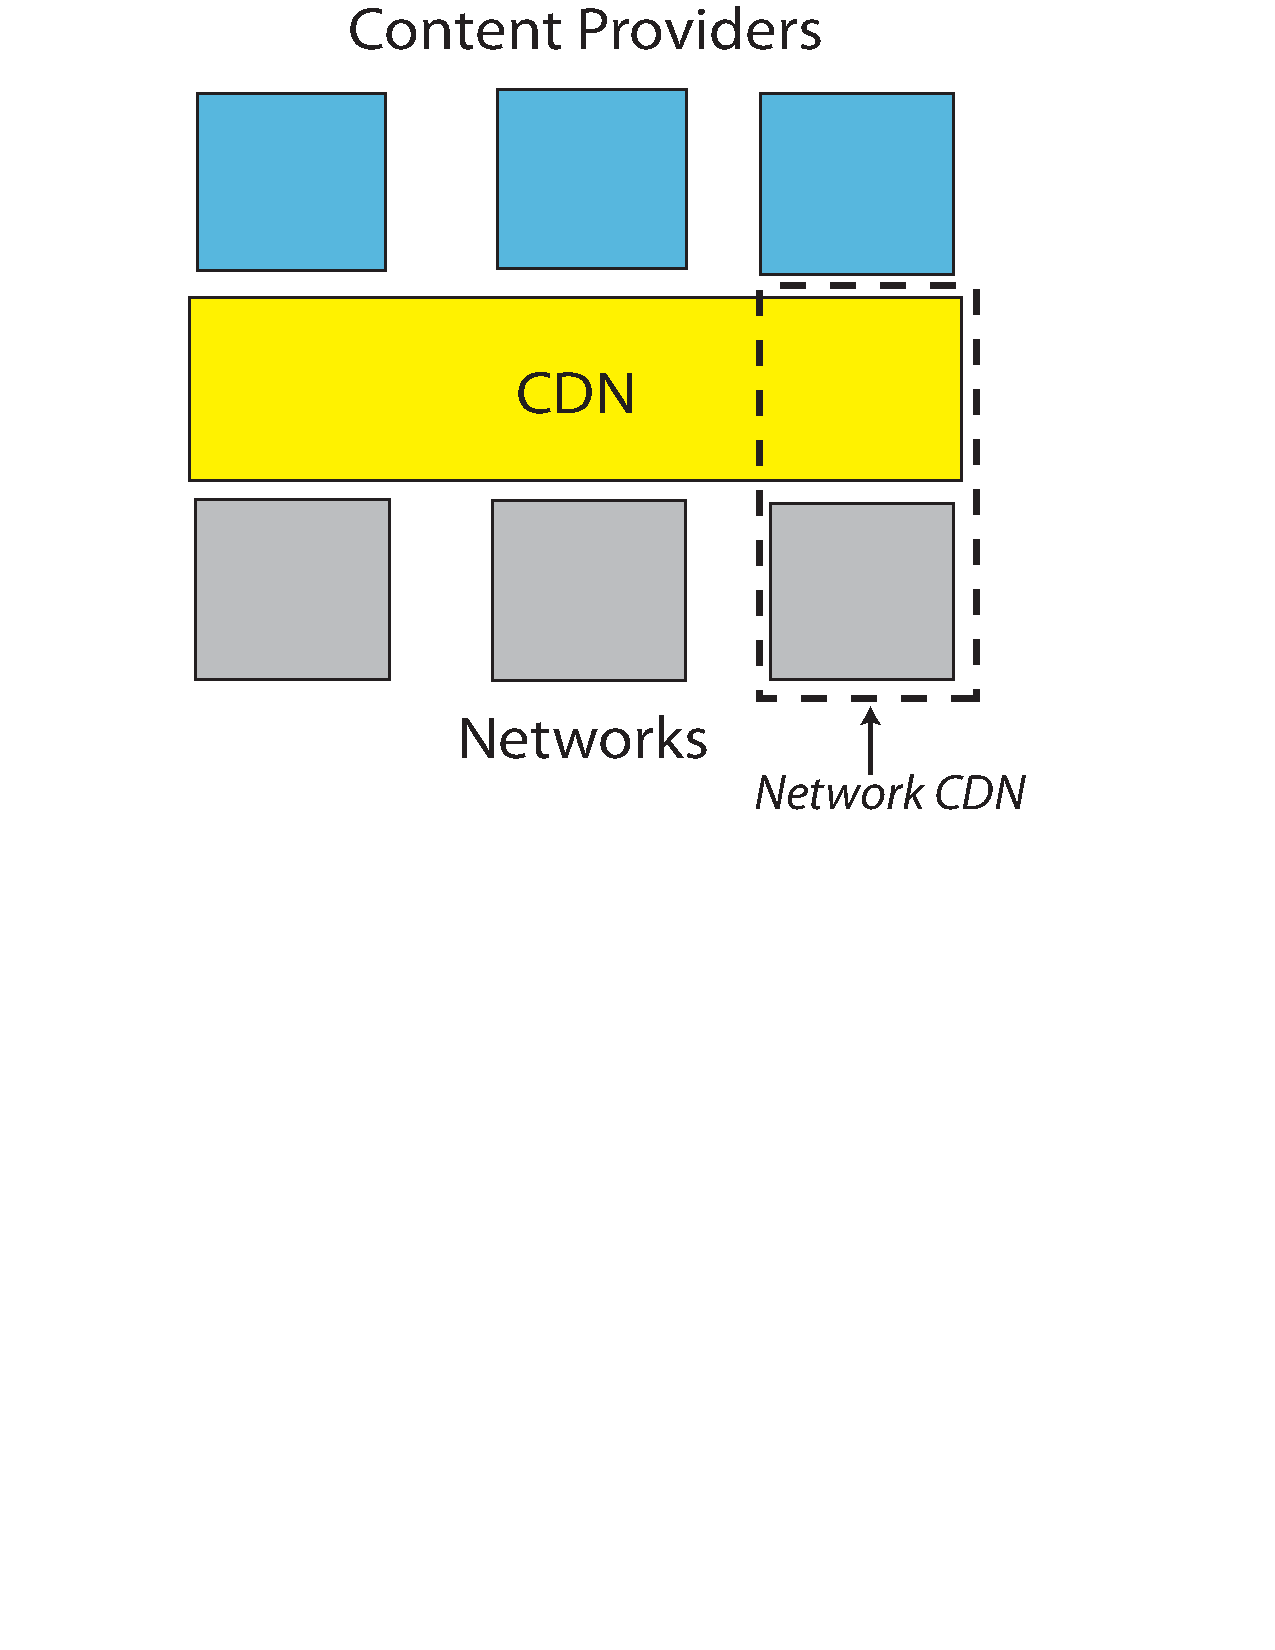
\includegraphics[height=2.5in]{ncdnpaper/NetworkCDN}}
\vspace*{-1.35in}
\caption{A tripartite view of content delivery.}
\vspace*{-0.25in}
\label{fig:networkCDN}
\end{figure}



As \ncp s control both the content delivery and network infrastructure, the costs and objectives of their interest are different both from a traditional CDN and a traditional ISP. In particular, an \ncp\ is in a powerful position to place content in a manner that ``shapes'' the traffic demand so as to optimize both network cost and user-perceived latency as illustrated using the example in Chapter \ref{ch:te-background}, Section \ref{sec:bg-ncdn}. Indeed, several recent works have alluded to the benefits of such joint optimization strategies in the context of cooperative or competitive interaction between ISPs and content providers \cite{P4P,JohariGameTheory,Jiang2009,catenew}. On the surface, an \ncp\ would appear to be the perfect setting for fielding joint optimization strategies as it eliminates potentially conflicting competitive interests. Nevertheless, \ncp s today continue to treat content delivery and traffic engineering concerns separately, operating the former simply as an overlay.

This disparity raises several research questions that form the focus of this chapter. How should an \ncp\ determine content placement, network routing, and request redirection decisions so as to optimize network cost and user-perceived latency? How much benefit do joint optimization strategies yield over simpler strategies as practiced today, and does the benefit warrant the added complexity?  How do content demand patterns and placement strategies impact network cost?  How do \planned\ strategies (i.e., using knowledge of recently observed demand patterns or hints about anticipated future demands) for placement and routing compare against simpler, \unplanned\ strategies?

Our primary contribution is to empirically analyze the above questions for realistic content demand workloads and ISP topologies. To this end, we collect content request traces from Akamai, the world's largest CDN today. We focus specifically on on-demand video and large-file downloads traffic as they are two categories that dominate overall CDN traffic and are significantly influenced by content placement strategies. Our combined traces consist of a total of 28.2  million requests from 7.79 million unique users who downloaded a total of 1455 Terabytes of content across the US over multiple days. Our main finding based on trace-driven experiments using these logs and realistic ISP topologies is that {\em simple, unplanned strategies for placement, routing, and redirection of NCDN content are better than sophisticated joint-optimization approaches}. Specifically,
\begin{itemize}
\item For NCDN traffic, simple \unplanned\ schemes for placement and routing (such as least-recently-used and InverseCap)  yield significantly lower (2.2--17$\times$) network cost and user-perceived latency than a joint-optimal scheme with knowledge of the previous day's demand\footnote{We use the term ``optimal'' when placement or routing is the solution of an optimization problem, but the solution may not have the lowest cost (for reasons detailed in Section \ref{sec:videodownload})}. 
\item NCDN traffic demand can be ``shaped'' by simple placement strategies so that  traffic engineering, i.e., optimizing routes with knowledge of recent traffic matrices, hardly improves network cost or user-perceived latency over \unplanned\ routing (InvCap).
\item For NCDN traffic, unplanned placement and routing is just 1\%-18\% sub-optimal compared to a joint-optimal placement and routing with perfect knowledge of the next day's demand at modest storage ratios ($\approx4$). % with simple optimizations such as content chunking and link-utilization-aware redirection.
\item With a mix of NCDN and transit traffic, traffic engineering does lower network cost (consistent with previous studies), but the value of traffic engineering substantially diminishes as the relative volume of NCDN traffic begins to dominate that of transit traffic.
\end{itemize}
\vspace{-0.08in}
%\item Future knowledge helps, i.e., demand-oblivious placement and routing is moderately worse compared to a joint-optimal placement and routing with perfect knowledge of the next day's demand at small to moderate storage ratios (<  2.2), but the difference reduces to less than 20\% at higher storage ratios  ($\approx$ 4). 

%\item Demand-oblivious placement and routing performs within 20\% of joint-optimal placement and routing with perfect knowledge of the next day's demand at a moderate storage ratios (\approx 4). 

%\item Simple hybrid strategies (partly demand-aware and partly demand-oblivious) do not improve upon a completely demand-oblivious strategy; and optimizations such as chunking do not qualitatively change our findings.


In the rest of this chapter, we first overview the \ncp\ architecture highlighting why it changes traditional ISP and CDN concerns (Section \ref{sec:ncdn-background}). Next, we formalize algorithms that jointly optimize content placement and routing in an NCDN (Section \ref{sec:optimize}). We then describe how we collected real CDN traces (Section \ref{sec:dataset}) and evaluate our algorithms using these traces and real ISP topologies (Section \ref{sec:ncdn-eval}). 

% We provide background material on content-aware traffic engineering for NCDNs  (Section~\ref{sec:background}). We then provide algorithms for content-aware traffic engineering that perform content placement, request redirection, and traffic routing to minimize MLU (Section~\ref{sec:optimize}).  Next, we evaluate our algorithms using extensive real-world traces from a large commercial CDN (Section~\ref{sec:empirical}). Finally, we present related work (Section~\ref{sec:related}) and conclusions (Section~\ref{sec:conclusions}).

%While traditionally networks lacked a direct relationship with content providers to deliver their content, the NCDN approach provides an avenue for networks to tap into that revenue stream. In addition, deploying an NCDN provides the additional benefit of higher performance for their subscribers that could form the basis for new differentiated services. As an example of this trend, consider the recent offering by Verizon that delivers HBO's content to FIOS TV subscribers

%Recent powerful trends are reshaping the simplified tripartite view of content delivery. A primary driver is the torrid growth of video and download traffic on the Internet.  Consider that a single major television show with a viewership of 50 million with each viewer watching a HD-quality stream of 10 Mbps generates 500 Tbps of network traffic! As traditional media such as television and movies migrate on to the Internet, the scaling of the network backbone to accommodate that traffic is a major technological challenge. This has necessitated the evolution of the {\em Network CDN\/} (NCDN, for short) that vertically integrates CDN functionality that provide scalability such as request  redirection and content caching with traditional network operations (See Figure~\ref{fig:networkCDN}).  A second economic driver for NCDNs is the desire of networks to monetize the ``bits'' that flow on their infrastructure. While traditionally networks lacked a direct relationship with content providers to deliver their content, the NCDN approach provides an avenue for networks to tap into that revenue stream. In addition, deploying an NCDN provides the additional benefit of higher performance for their subscribers that could form the basis for new differentiated services. As an example of this trend, consider the recent offering by Verizon that delivers HBO's content to FIOS TV subscribers.

%The mechanism for constructing an NCDN may vary from a complete turnkey solution where a traditional CDN deploys their service at the network's PoPs, to a software licensing solution where a traditional CDN licenses their software for the network to use, to the network building the CDN functionality themselves. 
%Independent of the mechanism, 

%NCDNs raise important scientific questions on how content delivery functionality impacts the traditional traffic engineering focus of networks.  While the two functionalities are performed separately today,  the trend towards NCDNs opens up for the first time the possibility of jointly optimizing content delivery and traffic engineering, as both are now controlled by the same business entity. To our knowledge, our work is the first to examine the rich possibilities that are opened up by this nexus.  {\em A primary contribution of this paper is that effective content delivery can simplify or even completely obviate the need for complex traffic engineering implemented by networks today. } 

%{\bf NCDN Architecture.} 
\begin{figure}
\vspace*{-0.7in}
\centerline{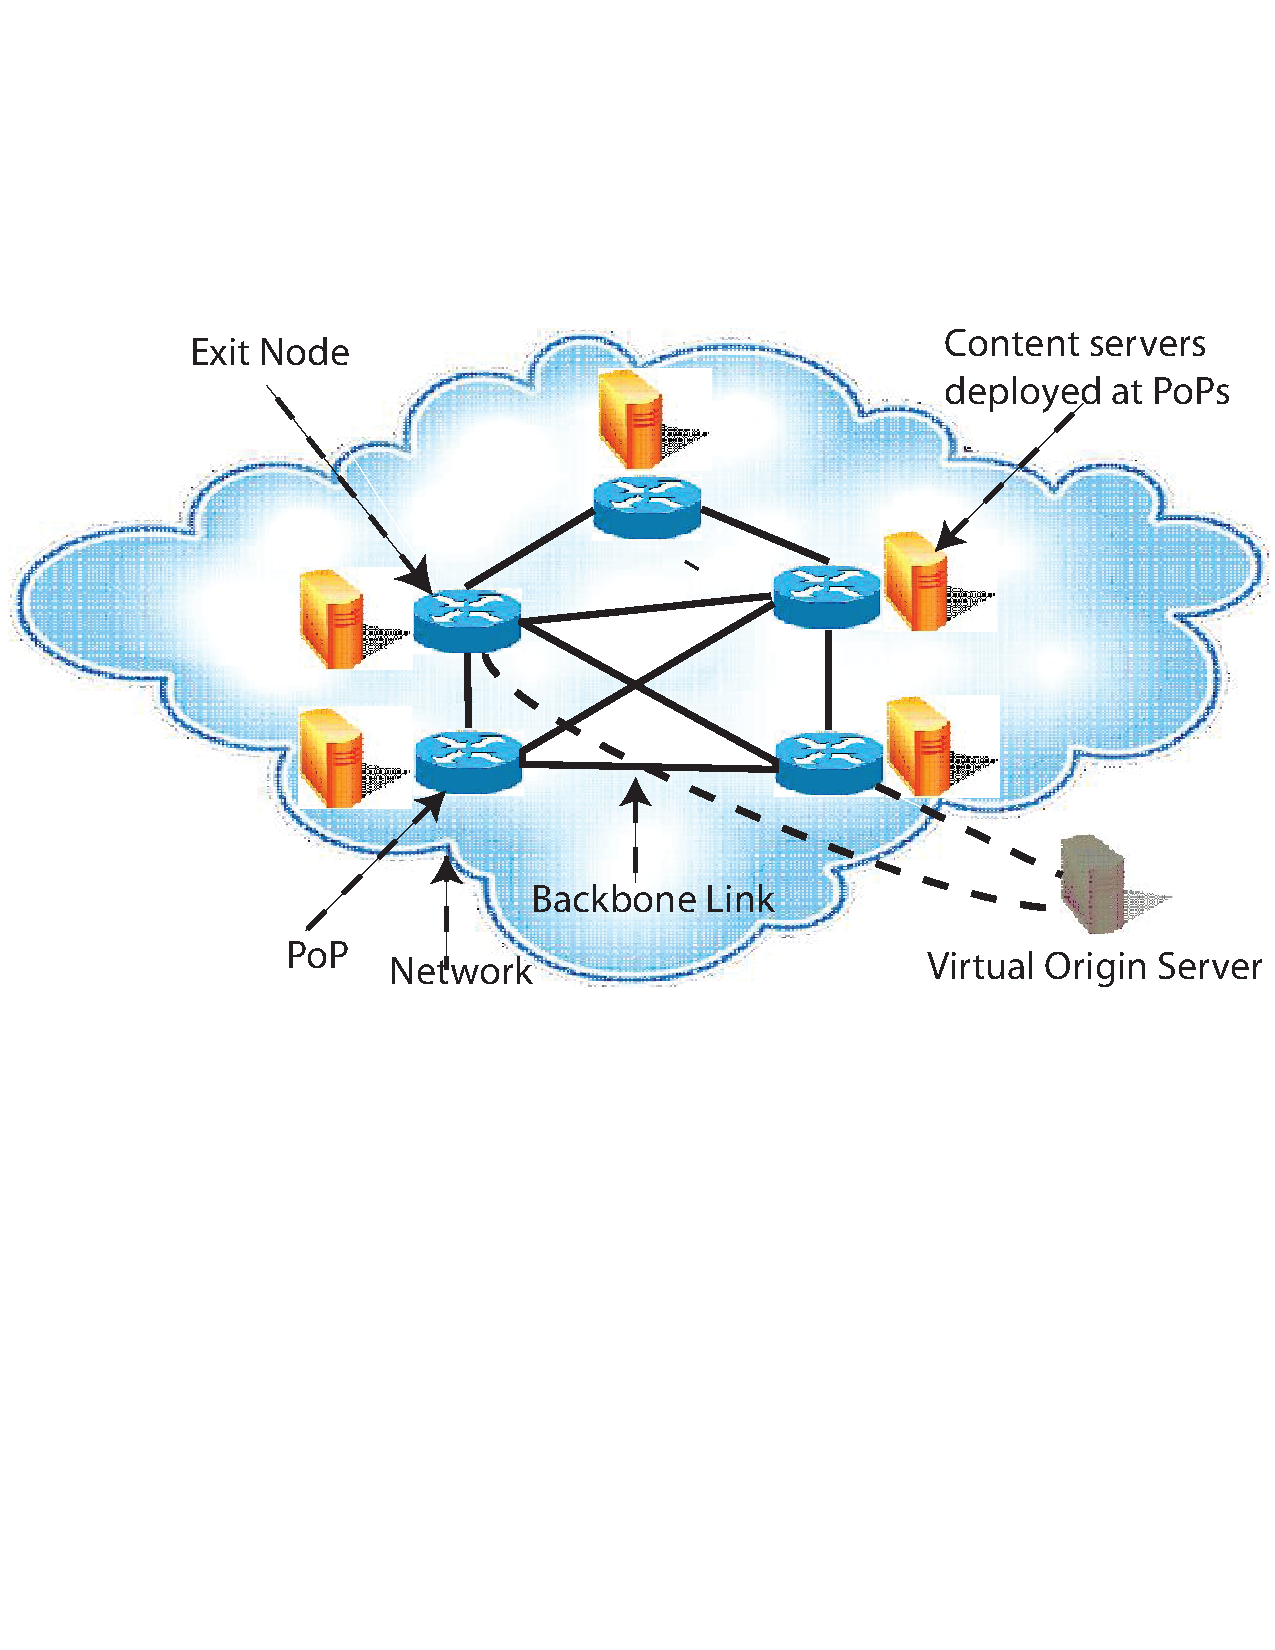
\includegraphics[height=3.5in]{ncdnpaper/NCDNArch}}
\vspace*{-1.3in}
\caption{NCDN Architecture}
\label{fig:NCDNArch}
\end{figure}
%A typical NCDN architecture follows closely the architecture\footnote{For a detailed treatment of the architectural components of a global CDN, the reader is referred to \cite{akamai-overview}.} of a global CDN, except that the content servers are deployed at PoP's within the network rather than globally across the Internet (See Figure~\ref{fig:NCDNArch}).   Further, an NCDN typically serves content only to downstream end-users and subscribers of the network, rather than to a global audience. Each content provider publishes all their content to {\em origin servers} that they maintain. The origin servers may be mirrored across different data centers on the Internet and these mirrors could be hosted external to the NCDN itself on a different network. 

%Each PoP is associated with the set of end-users downstream from it who request content, such as requests for web content, downloads, and video content. Thus each PoP can be viewed as a source of demand for content that must be satisfied either by the content servers local to the PoP,  or by downloading from a  content server at a different PoP, or by downloading the content directly from the origin. When an end-user requests a piece of content,  the request is first routed to the content servers deployed at the PoP to which the end-user is connected.  If a content server at that PoP has the requested content in their cache, it serves that content to the end-user. Otherwise, if the requested content is cached at another PoP in the network, the content is downloaded from that PoP and served to the end-user. Finally, if the content is not present in any content server in the network, it is downloaded directly from the origin servers of the content provider. 

%{\bf content delivery.}  The two key aspects of content delivery that we study are {\em content placement} that determines which piece of content is placed on content servers of which PoP (potentially with replication) and {\em request redirection\/} that determines which content servers are used to serve each requested piece of content.  Note that when a piece of requested content is present in content servers at multiple PoPs, the request redirection policy determines which PoP serves the request. 

%{\bf Traffic Engineering.} A key component of network operations is routing the traffic demands on the backbone network so as to enhance network performance and maximize the utilization of network resources \cite{fortz2002traffic}. More formally, given the topology of the network with link capacities and a demand matrix $D$ that specifies the traffic flow that must be routed between each pair of nodes (i.e., PoPs) $(s, t)$,  the goal of traffic engineering is to determine the path(s)  to route each such traffic flow such that a predetermined objective function is minimized\cite{fortz2000internet}.  The most common objective function is to minimize the maximum link utilization (MLU) in the network, where link utilization is the ratio of the traffic flow on that link and its capacity. The paths to route the traffic flows in the network are themselves constrained by the intra-domain routing protocol impmemented by the network. The protocol that is most widely used in practice is Open Shortest Path First (OSPF) where the network operator assigns weights to each link and the path used between $s$ and $t$ is simply the shortest path(s) between the nodes using the weights as the lengths of the links. Further, if a node has multiple outgoing links that each yield the same distance to the destination, traffic is split evenly between those links. A simple special case of OSPF that is commonly used is InverseCapacity routing (InvCap) where the OSPF weight of each link is statically set to be the inverse of its capacity.  More flexible than OSPF is the Multi-protocol Label Switching (MPLS) protocol. MPLS can implement any set of routing paths, since in principle the route of each packet can be specified in an independent fashion. However,  MPLS is more complex to implement compared to OSPF variants. Our critical observation is that effective content delivery can ``shape'' the traffic demand matrix $D$ in manner that simplifies or even obviates the need for complex traffic engineering.

%{\bf Our Contributions.} Need to write.

%{\bf Roadmap.} We provide background material on content-aware traffic engineering for NCDNs  (Section~\ref{sec:background}). We then provide algorithms for content-aware traffic engineering that perform content placement, request redirection, and traffic routing to minimize MLU (Section~\ref{sec:optimize}).  Next, we evaluate our algorithms using extensive real-world traces from a large commercial CDN (Section~\ref{sec:empirical}). Finally, we present related work (Section~\ref{sec:related}) and conclusions (Section~\ref{sec:conclusions}).

%The boundary between the entities which route traffic, i.e., Internet %service providers (ISPs), and the entities which publish content is %increasingly blurring in today's Internet with one progressively taking %the role of another. For example, top ISPs such as AT\&T, Level-3  and %Verizon  are also among the top content distributors and top content %distributors such as Comcast and manage their own networks. 

%We envision a network where the owner termed as \textbf{N}etwork and %\textbf{C}ontent \textbf{P}rovider (\textbf{\ncp})  can decide the %placement of content  at nodes in the network, in addition to choosing %the routes between nodes, as is done today.  Each user in the network %termed as \textbf{C}ontent \textbf{C}onsumer (\textbf{\cc}) can demand %any content provided by its \ncp.

%Since an \ncp\ manages network as well as content served through the network, it needs to solve problems faced by ISPs which manage traffic in their networks , as well as CDNs, which manage content from their clients. For example, where to place content? How many copies  of each content to place ? How to  determine routes  between nodes while keeping network links free from congestion ? How to load balance among servers at different PoPs?
%How to load balance between sets of servers across nodes?


%The task for an \ncp\ can be broken down into two sub-problems: (1) Network and storage capacity planning over a long term (2)  Managing content storage and network traffic on a day-to-day basis. In this work, our focus is the later problem. But we also study the effect of network and storage capacity available in the network on our results.


%There are three metrics of interest for an \ncp:  (1) Congestion of links in the network (2) 	Load on the servers at each PoP (3) Link latency between \cc's and content they are accessing.  An \ncp's strategy for content placement and routing affects all three metrics mentioned above. For example, replicating a very popular content at many locations in the network will reduce congestion, will distribute the load from servers at one PoP to multiple PoPs and  reduce the latency between \cc's and the content. 

%In this context, our work is motivated by the question: ``Which among content placement and routing plays a greater role in optimizing the metrics of interest for an \ncp?" We compare the performance of simple vs. sophisticated strategies for routing and for deciding content placement. 

%Based on our experiments using  traffic data from three ISPs, we conclude that optimizing content placement is considerably more important  than optimizing routing for an \ncp. A strategy which decides  content placement optimally while adopting a simple static routing performs much better than a strategy which uses a simple content placement with  an optimal routing; it even performs nearly identical to a strategy which makes both content placement and routing decisions optimally. 


%Our paper makes the following contributions:

%\begin{itemize}
%\item
%A  comparison of content placement strategies in terms of their network cost based on real world traces from a very large CDN including three major sources of Internet traffic - short video, long video and software downloads.
%\item
%hypothetical: A combination of static and dynamic placement strategies performs best or equally best for all three traces. Using a dynamic placement alone performs close to optimal for short videos, but is sub-optimal for other content types. Using a purely static placement strategy 
%\item
%hypothetical: Using the best content placement strategy along with a naive routing reduces network cost more than optimizing routing but using a significantly worse content placement strategy.
%\end{itemize}


%\ncp's  solution to these questions must consider the performance for users in the network, as well as cost incurred by \ncp.  From an \ncp's perspective the objective would be to minimize the capital expenditure cost  of storage and  links, assuming that operational cost does not rise on decreasing capital expenditure. From a \cc's perspective, the performance improves on reducing the delay between \cc\ and the node that is storing the content it is consuming.
%
%
%We split the network management problem for an \ncp\ into three problems: (1) which location/s is each content placed ? (2) which replicas for a content are used for  \cc's at a node ? (3) how is traffic routed between two locations ? 

 
% content management + network management 

%We take the first step towards designing a network management solution for the NCP by comparison four design choices for an 




%ISPs change routing in the network in response to changing traffic demands in order to reduce the congestion in the network. This process is called traffic engineering. Specifically, ISPs optimize the maximum link utilization metric (MLU) so as to reduce the link utilization of backbone links in the network which in turn is expected to minimize congestion. Traffic engineering is widely used by ISPs today and techniques for traffic engineering have seen a large body of work in the research community.

%If an ISP can place the content being distributed in the network, it can minimize congestion also by changing the content placement. Optimizing content placement includes deciding how many replica of each content to store in the network, where to place content in the network, and how to split traffic demand among multiple servers in the network. Changing content placement can modify the traffic on links in the network and therefore optimizing placement and help reduce MLU in the network. In particular, creating additional replicas can significantly reduce the traffic in the network since  content can be obtained from nearby locations. If a content is placed at the PoP which is requesting the content, the traffic demand for the content from that node vanishes. 

%Assuming that an ISP could optimize both content placement and routing, what should an ISP  optimize for traffic engineering.  To this end we compare traffic engineering schemes which belong to one of the following four categories: 
%(1) Simple Routing + Simple Placement: 
%(2) Optimal Routing + Simple Placement
%(3) Simple Routing + Optimal Placement
%(4) Optimal Routing + Optimal Placement

%We present linear programs to compute routing and placement for these traffic engineering schemes. Using two sets of ISP topologies and traffic matrices, we compare the performance of the above TE schemes.

%Our main conclusions from this work are as follows:
%\begin{enumerate}
%\item 
%Optimal Placement with a InvCap routing scheme (InvCapOptimalPlacement)  performs identical to the joint optimal solution of MLU and routing.
%\item
%Optimal routing coupled with a simple placement strategy performs sub-optimally compared to optimizing both placement and routing.
%\item
%Optimizing placement for content with local popularity gives up to a 10$\times$ reduction in MLU compared to other TE schemes.
%\end{enumerate}




%An ISP network where ISP is both the content distributor and the network service provider. In this case, ISP can optimize both routing as well as the content placement. We assume that the content placement allows a small degree of replication in the network, which provides location diversity for content in the network. An ISP seeks to maximize the traffic demand which can be served through its network. Therefore it optimizes MLU. 

%\textbf{hypothesis: placement benefits MLU more than routing}

%Our hypothesis is that placement is more important than routing to maximize the maximum served traffic demand in the network, that is optimal placement is more valuable than optimal routing. 

%\textbf{problem: How much replication is needed for optimal placement to perform close to optimal (placement + routing) ?}

%If this is indeed the case, then ISP can place content optimally in the network and perform a simple routing such as InvCap in the network.  Building up on our previous results, this would suggest that ISPs do not need to do any traffic engineering in the network. The next important question is that how much location diversity is needed to gain the benefits of optimal placement over optimal routing ?

%\textbf{problem: Which algorithm to use for placement?}
%
%- Optimal
%
%- Heuristic ?
%
%\textbf{problem: at what timescales can we compute placement ?}
%
%- 
%
%\textbf{conclusion: ?}
%
%just placement is good enough to get close to (optimal placement + optimal routing).
%
%
%2. Examples/results motivating optimal placement over routing
%
%3. Network model and algorithms
%
%3.1 Network model
%
%3.2 Joint Placement + Routing  : 
%
%- NP Hard
%
%- Linear program for this problem
%
%- Rounding techniques
%
%3.3 Fixed routing + Optimal Placement 
%
%- NP Hard 
%
%- Changes to Linear program
%
%- Rounding techniques
%
%3.4 Simple Placement Strategies
%
%
%
%4. Evaluation
%
%- file popularity distribution : zipf-like, homogenous
%
%- file size : s
%
%4.1 Effect of file popularity distribution across nodes
%
%- homogenous : gravity
%
%- heterogenous : gravity
%
%- mix of homo and hetero
%
%4.2 Effect of traffic demand
%
%- gravity
%
%- 
%
%5. Related work
%
%6. Conclusion



%\textbf{Previous Intro}
%
%The goal of the project is to develop algorithms for traffic engineering when the ISP can place content as well route traffic. This problem can be divided into two sub problems: (1) placing  content optimally in the network  (2)  routing optimally when the content location as well as the traffic demand in the network is known.
%
%To our knowledge, the first question, i.e., optimally placing content to optimize a traffic engineering metric has not been analyzed in previous work. The solution to the second problem can be obtained using linear programs which are described in Section \ref{sec:linearprograms}.
%
%Problems:
%
%1. For a set of traffic demands from a set of sink nodes, optimize routing when (1) there is only one type of content (2) there are multiple types of content. Vary the number of locations.
%
%2. For a set of traffic demands from a set of sink nodes, optimize C = w * COST(content placement)/OPTCOST + (1- w) * MLU(routing)/OPTMLU
%

%
%Sequence of steps for optimal MLU:
%
%\begin{enumerate}
%\item
%Show that finding the optimal placement problem to optimize MLU is NP-hard.
%\item
%Compare the performance of heuristic algorithms for different levels of diversity: Random, probabilistic rounding, local search.
%\item
%Compare the performance of heuristic algorithms when there are different types of content.
%\end{enumerate}


%\section{Background}
%
%\subsection{Changing Internet}
%
%\subsection{Multiple ways to engineer traffic}
%
%\subsection{Challenges}


%An important criterion in designing a network management scheme is how often can we change the network configuration: The placement can only be changed in the order of days since it incurs a huge overhead in terms of time and network bandwidth to change the content placement. The flow splits among multiple locations and the routing can be changed in the order of minutes or hours since they only require changing few parameters in the network, the resulting change can be quickly realized. Therefore, we assume that a placement operation runs on a slower time scale than computing routing or changing flow splits in the network.

%Flow splits among multiple locations can be done in multiple ways for the same placement of content. But, we combine actions (1) and (2) into one action. This implies (1) and (2) are (1) and (2) happen together in the network and at a slower time scale than changing the routing in the network.


%\documentclass{sig-alternate-10pt}	
%\documentclass[letterpaper,twocolumn, 10pt]{article}
%\usepackage{usenix,endnotes}

%\renewcommand*\rmdefault{ppl}
%\selectfont
\usepackage{array}
\usepackage{caption}
\usepackage{subcaption}
\usepackage{verbatim, soul}
\usepackage{comment,pifont,array,url,amsmath,multirow,latexsym,tabularx}
\usepackage{ifpdf,rotating,colortbl}
\usepackage{graphicx}
\usepackage[lined,linesnumbered,noend]{algorithm2e}
\usepackage{wrapfig}
\usepackage{xspace}
\usepackage{url}
\usepackage{bbm}
 \usepackage{wrapfig}
 \usepackage{sidecap}
 \usepackage{hyperref}
\usepackage{booktabs}
\usepackage[font={sl,small},labelfont=bf,skip=7pt,labelsep=quad]{caption}


\newcommand{\TBD}[1]{\textcolor{red}{[\bf{TBD:}#1]}}
%	
%} % will appear in bold font and will be set to null eventually.
\newcommand{\tbd}[1]{\footnote{\bf{TBD:}#1}}
\newcommand{\eat}[1]{}
\newcommand{\vsp}{\vspace{-0.1in}}


\newcommand{\shrink}{Shrink}
\newcommand{\cdc}{CDC}


\begin{document}
\title{\shrink: Quantifying and Leveraging Energy-Performance Tradeoff in Content Datacenters}


%\author{
%{\rm Abhigyan Sharma$^\dagger$ \quad Vijay Pasikanti$^\dagger$ \quad Arun Venkataramani$^\dagger$ \quad Ramesh Sitaraman$^{\dagger\star}$}\\
%$^\dagger$University of Massachusetts Amherst\quad $^\star$Akamai Technologies
%} % end author

\maketitle

%!TEX root = New.tex
\begin{abstract}

Many datacenters are primarily used for content delivery. These datacenters are typically lightly loaded during normal operation, and hence have significant potential for saving energy. However, saving energy by shutting off servers could reduce cache-hit rates and by shutting off network components could increase datacenter network congestion; both events hurt user-experience. Due to these perceived risks, operators leave entire datacenters in an always on state foregoing all energy savings.

Towards the goal of saving energy in data center networks, we present \shrink, a cluster manager that makes power management decisions for networks and servers in a coordinated manner  to maximize energy savings, and  decides load balancing and traffic engineering  to ensure a minimal impact on user-perceived performance.
Further, \shrink\ orchestrates content transfers before server shutdown events to minimize the impact of server shutdown on cache hit rates.  We implement a prototype of \shrink\ using \TBD{TBD} library, and conduct extensive trace-driven evaluation using traces from a large CDN. Our results show that \shrink\ can reduce energy consumption by TBD-TBD\% with minimal impact on user-perceived performance and saves energy within TBD\% of the optimal strategy.

\end{abstract}
%!TEX root = Main.tex
\vsp
\section{Introduction}
\label{sec:intro}
``Mobile'' has long arrived, but the Internet remains unmoved. Today, there is roughly one cellphone per human; the number of smartphones sold last year alone roughly equals the number of wired hosts on the Internet \cite{gartner}; and the total traffic originated by mobiles is poised to approach that by wired devices \cite{cisco-vni}. However, the current Internet continues to operate as it did when dominated by tethered hosts, simply ignoring frequent endpoint mobility.

Today, an application developer can not easily initiate communication with a smartphone even when it has a public IP address as there is no global infrastructure support for locating it. Applications like smartphone notification systems, playback video, or cloud storage have to develop application-level support to enable a seamless experience for their users even as they change addresses several times a day, or let connections break (as popular VoIP apps do today).   The lack of intrinsic support for mobility means that developers are forced to redundantly develop and maintain common-case functionality. Furthermore, we are paying an unknowable price in terms of long-term growth and innovation by straitjacketing communication initiation to be unidirectional.

%The lack of intrinsic support for mobility means that we are paying an unknowable price in terms of stymied application innovation and growth by forcing developers to redundantly develop common-case functionality, and forcing communication initiation to be mostly unidirectional.

%A mobile user might reasonably expect that a voice-over-IP call she initiated through one WiFi network would continue uninterrupted if she switched to a different WiFi or  cellular network; or expect a file transfer she initiated at home on her laptop to resume when she opens it at work in a disruption-tolerant manner. Today, one can not easily initiate communication with a smartphone (even when it has a publicly visible IP address) because there is no global infrastructure support for locating it. Of course, application developers can design around these limitations, as do applications like Skype\tbd{I don't think Skype actually supports this today. Netflix maybe a better example.}, Dropbox, and smartphone notification systems respectively for the above scenarios. However, the lack of intrinsic support for mobility means that we are paying an unknowable price in terms of stymied application innovation and growth by forcing developers to redundantly develop common-case functionality, and forcing communication initiation to be mostly unidirectional.

%Many before us have criticized the Internet architecture's poor support not only for mobility but also for multihoming \cite{HIP,LISP,HAIR}, content retrieval \cite{DONA,LNA,CCN}, and security \cite{AIP,XIA,MobilityFirst-UMASS}. A common criticism is the Internet's so-called conflation of identity and location. The Internet uses an IP address both to represent the identity of an interface as well as its network location, which is problematic for mobility (same identity, changing locations) and multihoming (single identity, multiple locations) of devices, services, or content. Applications today are forced to know and care about changing IP addresses as the transport and network layers only provide a primitive to establish  connections between IP addresses, not application-friendly names. It is commonly accepted wisdom that a cleaner separation of identity and location is instrumental to fixing these problems.

%Many before us have criticized the Internet architecture's poor support not only for mobility but also for multihoming \cite{HIP,LISP,HAIR}, content retrieval \cite{DONA,LNA,CCN}, and security \cite{AIP,XIA,MobilityFirst}. A common criticism is the Internet's so-called conflation of identity and location. The Internet uses an IP address both to represent the identity of an interface as well as its network location, which is problematic for mobility (same identity, changing locations) and multihoming (single identity, multiple locations) of devices, services, or content. Applications today are forced to know and care about changing IP addresses as the transport and network layers only provide a primitive to establish  connections between IP addresses, not application-friendly names. It is commonly accepted wisdom that a cleaner separation of identity and location is instrumental to fixing these problems.

Many before us have criticized the Internet architecture's poor support for mobility as well as multihoming \cite{HIP,LISP,HAIR,MobilityFirst}. A common criticism is the Internet's so-called conflation of identity and location, i.e., the use of an IP address both to represent the identity of an interface as well as its network location, which is problematic for mobility (same identity, changing locations) and multihoming (single identity, multiple locations). It is commonly accepted wisdom that a cleaner separation of identity and location is instrumental to fixing these problems. However, the Internet does separate identities (domain-names) from network locations (IP addresses) through DNS. Most high-level programming languages also provide syntactic sugar to \verb+connect+ to names remaining oblivious to IP addresses; and %name owners can and do employ managed DNS services or CDNs to return the best-positioned network location corresponding to multi-homed names. 
techniques from a long line of work on connection migration could be employed to seamlessly handle mid-connection mobility.

But a key missing element from this package today is a distributed name resolution infrastructure that can scale to orders of magnitude higher update rates than envisioned when DNS was created. To appreciate the envisioned scale, consider tens of billions of mobile identifiers changing network addresses at least tens of times per day. DNS's heavy reliance on TTL-based caching, a key strength recognized by its creators, researchers, and operators alike, poses a significant handicap by increasing update propagation delays, load on name servers, and overall client-perceived latency. It is not uncommon for DNS update propagation to take a day or more, resulting in long  outage times when online services have to be moved unexpectedly, prompting cries for help on operator forums \cite{serverfault,dns-long-update}. A less widely noted limitation of DNS is its reliance on hierarchical names for scaling via federation and its single root of trust, which constrains mobile applications from selecting arbitrary application-specific names (as elaborated in $\S$\ref{sec:whyNotDNS} and $\S$\ref{sec:design_overview}).

 %   Mobile has arrived, but the Internet is still static.

%    Reason 1: identity-location conflation. A number of solutions proposed to address this.

%    Reason 2: identity-location conflation would not be that problematic with an efficient resolution infrastructure. The Internet does separate human-readable ``names" from ``locations" or IP addresses through DNS. However, the design of the DNS resolution infrastructure implicitly assumes rare mobility. Indeed, Mockapetris and Dunlap allude to this by justifying the design decision of departing from the Xerox PARC Grapevine system... quote here.


Our position is that seamless support for mobility requires a logically centralized global name service that rapidly translates identities to locations irrespective of how exactly identities and locations are individually represented. Our primary contribution is the design, implementation, and evaluation of \auspice, a distributed system that helps address this challenge. Compared to today's ICANN/DNS-based approach, our approach cleanly separates name resolution from adjudication and certification issues ($\S$\ref{sec:design_overview}). \auspice\ is also deployable as a managed DNS provider in today's Internet; compared to them, a key strength of \auspice\ is a {\em demand-aware} replica placement engine that significantly reduces the {\em time-to-connect} to mobile destinations in a cost-effective manner. Under light load, \auspice's demand-aware replica placement aggressively uses available resources to massively replicate name records, while under heavy load, it carefully controls the number and choice of replica locations based on the read-write patterns and pockets of high demand for each name.

%low lookup latency, low update cost, and high availability.  \auspice\ achieves low-latency by inferring pockets of high demand for a name so as to create replicas of  for that name close to them. \auspice\ achieves low latency,  low update cost,  and high availability using a placement optimization algorithm that (1) controls the number of replicas based on the observed read and write rates, and (2) determines where to place replicas based both on the inferred pockets of demand and the aggregate load at node locations near those pockets. 



We have implemented a prototype of \auspice\ as a geo-distributed key-value store to serve as a flexible name resolution service for the current Internet as well as several ``future'' Internet or endpoint architectures such as MobilityFirst\cite{MobilityFirst}, HIP\cite{HIP}, or XIA\cite{XIA}. We have extensively evaluated \auspice\  using a combination of Planetlab, emulation clusters, and Amazon EC2.  Our contributions are as follows.
\begin{enumerate}
\item A case for a global name service as an indispensable part of any Internetwork design with intrinsic support for high mobility ($\S$\ref{sec:case}).
\vsp
\item \auspice, a scalable, geo-distributed, federated global name service that significantly reduces the time-to-connect under any given resource constraints despite high mobility and arbitrary endpoint identifiers ($\S$\ref{sec:design},$\S$\ref{sec:eval}). 
\figvsp
\item A proof-of-concept demonstration of intrinsic support for---{\em(i)} all four types of endpoint mobility; {\em(ii)} novel context-aware delivery primitives that generalize name- or address-based communication---over the current Internet as well as MobilityFirst \cite{MobilityFirst} ($\S$\ref{sec:e2e}). 
\vsp
\item Comparison against several best-of-breed managed DNS services showing that \auspice's  demand-aware approach significantly lowers time-to-connect and/or update cost even for today's (hardly mobile) domain names ($\S$\ref{sec:managed}).
\vsp
\end{enumerate}
\vsp

To provide a historical perspective, until the early 80s, the Internet relied on a system called \verb+HOSTS.TXT+ for name resolution, which was simply a centrally maintained text file distributed to all hosts. The current Internet's distributed DNS  arose in response to the rapidly increasing file size and distribution costs. Mockapetris and Dunlap \cite{DNS} point to TTL-based caching to reduce load and response times as a key strength, noting that ``{\em{the XEROX system {\em [Grapevine \cite{grapevine}]} was then ... the most sophisticated name service in existence, but it was not clear that its heavy use of replication, light use of caching ... were appropriate}}''. We have since come a full circle, turning to  active replication ($\S$\ref{sec:whyNotDNS}) in \auspice\ in order to address the challenges of mobility, a concern that wasn't particularly pressing  in the 80s. Compared to classical systems like Grapevine or ClearingHouse, \auspice\ enables support for automated {\em demand-aware} replica placement for {\em arbitrary names} (using several modern design elements such as consensus, the key-value abstraction, self-certifying names, consistent hashing, etc).  \auspice, through its support for context-aware delivery, is also a step towards addressing some of the challenges to which Lampson alludes on representing ``descriptive names" \cite{Lampson}.


\eat{
\emph{Low update cost:} \auspice\ reduces updates costs by nearly an order of magnitude over a replicate-everywhere strategy in a live deployment and yet achieves nearly identical lookup latencies.
\item
\emph{Load balance:} Over a wide range of loads, \auspice's achieves 2X - 4.5X lower lookup latencies over a random replication scheme, and  5.4X - 11.2X lower latency than a DHT-based replication scheme. Due to its lower update costs, \auspice\ can sustain 18$\times$ higher loads than a replicate everywhere strategy.
}

%\begin{itemize}
%\item
%Locality-aware placement helps \auspice\ achieve 5$\times$ lower median lookup latency than a DHT-based replication scheme. 
%\vspace{-0.1in}
%\item
%\auspice\ reduces updates costs by nearly an order of magnitude over a replicate-everywhere strategy in a live deployment and yet achieves nearly identical query latencies.\vspace{-0.1in}
%\item
%\auspice's load-aware design achieves 1.2$\times$-3.3$\times$ lower lookup latencies than a locality-unaware scheme over a wide range of load scenarios.\vspace{-0.1in}
%\item
%\auspice\ achieves  DNS lookup latencies comparable to a leading managed DNS provider today even with only one third the number of name resolvers.
%\end{itemize}

%\begin{enumerate}
%\item  \auspice's locality-aware and load-aware replication achieves  5$\times$ lower latency than Codons, a proposed DHT-based replication alternative to DNS.
%\item \auspice\ reduces update costs
%\end{enumerate}
\eat {

The Internet's tremendous success and our maturing realization of its shortcomings have attracted significant research attention towards a clean-slate redesign of the Internet's architecture (e.g., NSF FIND \cite{FIND}, GENI\cite{GENI}, FIA\cite{FIA}). A number of the shortcomings of the current Internet can be traced back to issues related to {\em naming}, a central component of any distributed system design. In the current Internet, network entities are identified using IP addresses and the Domain Name System (DNS) resolves human-readable end-host names to IP addresses. Although this design has proven to be surprisingly malleable, it suffers from two sets of fundamental problems, both of which are  exacerbated by the the exponential growth of mobile devices and applications today.


The first results from the conflation of identity and location within an IP address, a design decision roundly criticized by many \cite{ROFL,Saltzer:1993:NBN:RFC1498,HIP,FARA,LNAI}. Using an IP address to identify a network interface as well as the network location of that interface complicates {\em mobility}---when the location changes but not the identity---and {\em multihoming}---when a single identity simultaneously resides at multiple locations---e.g., being simultaneously connected to a cellular and WiFi access network. With roughly 5 billion mobile devices worldwide today \cite{gartner}  (over a billion of which are IP-capable) compared to barely a billion tethered hosts \cite{CIA}, mobility and multihoming are the norm, not an exception. Conflating identity and location also poses a serious but  less widely acknowledged security challenge, namely, verifying that an interface indeed has the identity it claims. Unlike human-readable names that are bound to public keys by trusted certification authorities in order to enable application-level authentication today, IP addresses are harder to certify, especially when they change many times a day. As a result, we largely make do today with application-level security over a network that can be easily rendered unavailable by spoofing or hijacking of IP addresses.



The second results from the architecture of DNS, a critical part of the Internet's core infrastructure. The design of DNS in the Internet's early days implicitly assumed tethered hosts or infrequently changing addresses to be the common case, an assumption evident in its heavy reliance on caching and timeout-based invalidations for scalability. An inevitable consequence of this design is that unanticipated updates to DNS resource records are slow; more than 40\% domain names have a TTL of a day or more \cite{codons}. Even for slow-changing records, DNS lookup times constitute a significant fraction of user-perceived response times, e.g., over 30\% of web objects incur a DNS lookup latency of over a second \cite{Jung,Huitema}. Deploying more passive local name sever caches can reduce lookup latencies, but this benefit comes at the cost of further increasing update propagation delays or update load in the system. These and other problems with DNS such as poor load balance and responsiveness to changing demand patterns, vulnerability to denial-of-service attacks, etc. have been well documented by researchers \cite{Pappas,codons,Brownlee,dnssec}.

Our primary contribution is the design and implementation of a global name service that addresses the above problems. This global name service is a central component of MobilityFirst, a clean-slate future Internet architecture that is primarily motivated by the dual concerns of {\em mobility} and {\em security}.
%two concerns that are remarkable both for their absence in the design philosophy underlying the current Internet \cite{Clark88} as well as their immense importance today. 
MobilityFirst cleanly separates identity and location using a {\em globally unique identifier} (GUID) that, unlike an IP address, is by design devoid of location or any other structured information. Information about a GUID's location or {\em network address} (NA) is maintained by the resolution service. Both GUID and NA are {\em self-certifying}, i.e., they are one-way hashes of public keys, allowing any network entity to authenticate an entity claiming to possess a GUID or NA. Thus, the structureless nature of these identifiers enhances mobility as well as security. Section \ref{sec:MF} describes how the name service helps efficiently support a number of other functions such as multihoming, incoming traffic engineering, content retrieval, network mobility, multicast, etc.

%Key feature: low response times while respecting capacity constraints and consistency requirements. TBD.

A critical distributed systems challenge in realizing a global name service that supports mobility at scale  is the design and implementation of the infrastructure that quickly resolves identifiers to network addresses. To appreciate the scale, consider 10 billion identifiers (for mobile devices, services, content identifiers, or entire networks such as vehicular networks) moving across a 100 network addresses per day, i.e., a load of a million/sec for updates alone. Furthermore, the name service should process lookup queries quickly, requiring queries to be directed to a nearby replica that holds a consistent replica of the corresponding resource records. Finally, the service should balance the aggregate load across all names across the geographically distributed locations of the global name service. 

Our proposed solution to achieving all of the goals above---low latency, low update cost, and load balance---is a placement engine \auspice, that {\underline{\bf au}}tomates {\underline{\bf s}}ervice {\underline{\bf p}}lacement {\underline{\bf i}}n {\underline{\bf e}}lastic {\underline{\bf c}}louds. The \auspice\ engine is flexible in that it enables automated placement for cloud-hosted services that are more general (and in widespread use today) than name resolvers in a future Internet architecture. To ensure low response times, \auspice\ dynamically spawns or migrates service replicas close to pockets of high demand. To ensure low update cost and load balance under capacity constraints, \auspice\ controls the number and placement of service replicas using heuristic algorithms that are uncoordinated across services or a global optimization algorithm coordinated across all services by the hosting service provider.

We comprehensively evaluate \auspice\ using an implemented prototype on Planetlab and Amazon EC2. Also design custom simulator. Validate simulator. Case studies and results preview. TBD.

\paragraph{Roadmap} The rest of this paper is organized as follows. Section \ref{sec:MF} presents the naming subsystem in the MobilityFirst Internet architecture. Section \ref{sec:auspice} presents the design goals and architecture of an automated service replica placement system, \auspice, for geo-distributed cloud-hosted services and the instantiation of a global name service using it. Section \ref{sec:eval} describes the datasets used and the experimental evaluation of \auspice. Section \ref{sec:related} describes related work and Section \ref{sec:concl} concludes.

}


%!TEX root = New.tex
\chapter{Background}
\label{ch:background}
\eat{
\begin{itemize}
\item
More than a literature review
\item
Organize related work - impose structure
\item
Be clear as to how previous work being described relates to your own.
\item
The reader should not be left wondering why you've described something!!
\item
Critique the existing work - Where is it strong where is it weak? What are the unreasonable/undesirable assumptions?
\item
Identify opportunities for more research (i.e., your thesis) Are there unaddressed, or more important related topics?
\item
After reading this chapter, one should understand the motivation for and importance of your thesis
\item
You should clearly and precisely define all of the key concepts dealt with in the rest of the thesis, and teach the reader what s/he needs to know to understand the rest of the thesis.
\end{itemize}
}

This thesis builds on prior research in three areas: traffic engineering, content delivery, and the interaction of the two. We first review the major classes of traffic engineering strategies (Section \ref{sec:bg-te}). Next, we discuss common techniques used by content delivery systems, including strategies for content placement and for request  redirection (Section \ref{sec:bg-cdn}). Finally, we survey research on the interaction between network and content delivery, and find that the interaction between traffic engineering and either overlay routing or request redirection have been the focus of past research (Section \ref{sec:bg-interaction}).



\section{Traffic engineering}
\label{sec:bg-te}

The goal of traffic engineering (TE)  is to avoid congestion hotspots in the network by optimizing routes based on network topology and expected traffic demand. In the context of large Internet service provider (ISP) networks, traffic engineering decides both intra-domain (within the ISP) and inter-domain routing (across ISPs). We focus here on intra-domain routing and refer the reader to  \cite{Feamster2003,rexford} for a survey of inter-domain traffic engineering. 





We classify traffic engineering schemes based on the frequency at which they update routing. By this attribute, TE schemes can be grouped into three categories: (1) \emph{Demand-oblivious TE} uses static routes that are seldom updated \cite{Cohen,Racke}. (2) \emph{Demand-aware TE}  updates routes periodically, e.g., every few hours or every few days, based on recent history of traffic demand \cite{fortz2000internet,fortz2002traffic}. (3) \emph{Online TE} updates routes at timescales of hundreds of milliseconds, reacting instantaneously to traffic demand changes \cite{TEXCP}.

TE schemes are evaluated based on link utilization based metrics, e.g., a widely used metric is maximum link utilization \cite{COPE}. A TE scheme is usually compared against the optimal solution that minimizes the given metric by solving a multi-commodity flow optimization  \cite{TEXCP,fortz2000internet}.
By this measure, oblivious routing schemes perform poorly and can be shown to be arbitrarily worse compared to the optimal strategy  \cite{fortz2000internet}. For many ISPs networks, simple oblivious routing schemes are sub-optimal by a small constant factor  \cite{COPE,MultiTM,TEXCP}.
Offline TE schemes, while sub-optimal, perform superior to oblivious TE schemes. e.g., Fortz and Thorup show that   offline TE delivers up to 2$\times$ better on AT\&T network backbone. Online schemes have been shown to achieve near-optimal performance, but they are rarely used in production networks.

In practice, offline TE based on Open Shortest Path First (OSPF) and Multiprotocol Label Switching (MPLS) are commonly used  \cite{COPE,MultiTM,fortz2000internet,MPLS2}. Routes computed by OSPF traffic engineering must follow shortest-weight paths, therefore OSPF TE provides limited functionality to split traffic among multiple paths. 
MPLS TE overcomes this limitation by enabling traffic between two nodes to be split  in arbitrary ratios among multiple paths.
Therefore, MPLS TE gives better results than OSPF TE  \cite{COPE,MultiTM}.



Prior work on traffic engineering is based primarily on evaluation of link utilization based metrics, and has largely ignored the impact of traffic engineering on user-perceived performance. Further, the comparison of TE schemes has not taken into account the interaction with content delivery. This thesis contributes in answering these questions. In Chapter \ref{ch:beyondmlu}, we provide a comparison of traffic engineering schemes focusing on user-perceived metrics such as file download times, and VoIP call quality. In Chapter \ref{ch:beyondmlu} and Chapter \ref{ch:ncdn}, we evaluate TE schemes while accounting for the interaction between TE and content delivery and show that this interaction helps simpler TE schemes, such as oblivious TE or OSPF TE, perform closer to the optimal TE strategy in terms of user-perceived metrics as well as TE metrics.

%Server shutdown policies that concentrate traffic on the smallest possible subset of network topology indeed enable maximum network energy savings. 

%In Chapter 5, we show that server shutdown policies that concentrate traffic on the smallest possible subset of network topology indeed enable maximum network energy savings. 



%Network energy savings due to energy-aware traffic engineering depends on traffic patterns in the network, traffic patterns that are assumed to be fixed. In the case of CDN data centers, traffic patterns could be shaped by load balancing decisions and server shutdown policies. In Chapter 5, we investigate TE strategies that coordinate with datacenter load balancing decisions and server shutdown policies, and yield greater network energy savings than shown by prior work.

%We hypothesize that  there exists potential for more network energy savings in datacenters than shown previously, provided techniques for saving server energy work in coordination with those for saving network energy. 

%\textcolor{red}{How much energy could be further saved in scenarios where content placement flexibility exists?}

%The above discussion has focused more on traffic engineering in wide-area networks. Traffic engineering in data center networks is another very active research area and we refer the reader to  \cite{,,} for few recent papers.

%In comparison to approaches that optimize routing for a given traffic matrix, this paper shows that a joint optimization of content placement and routing for content-serving clusters yields greater network energy savings.

\section{Content delivery}
\label{sec:bg-cdn}
Content delivery systems seek to provide a high-quality experience to users accessing content in all regions  at all times. A canonical example of a content delivery system is a content delivery network (CDN). State-of-the-art CDNs operate geo-distributed datacenters, and use a combination of edge caching, intelligent server selection, and path and protocol optimizations for delivery of several types of content, e.g., video, bulk downloads, and interactive websites \cite{DilleyMPPSW02,akamai-overview}. Given their geo-distributed deployment, the decisions of content placement, i.e., locations at which a content is placed, and request redirection, i.e., which location is best positioned to serve a user's request, are central to the functioning of a CDN.

%The design of a content delivery system must consider the unpredictable nature of the Internet and of content workloads. The unpredictability arises from changes in network conditions, sudden spikes in content popularity, as well as malicious traffic generated by DDoS attacks. To provide quick response to these events, content delivery systems must use algorithms that are computationally efficient. Content delivery systems of today use distributed heuristics, often trading optimality for efficiency, to ensure high-quality user experience in all regions at all times.

\subsection{Content placement}
\label{sec:placement}
Placement strategies depend on whether content is static or dynamic. 
Dynamic content has limited cacheability therefore placement  strategies for static content are not always applicable for dynamic content.

\subsubsection{Static content placement}
\label{sec:static}
Static content, such as videos, audio, images and software updates, contribute to a vast majority of traffic in the Internet \cite{nielsen-video-growth,cisco-videogrowth}.  The placement of static content is commonly handled by a caching strategy. A simple and widely used caching strategy is least recently used (LRU) cache replacement  \cite{wessels2009squid}. Caching strategies are effective because they exploit geographic and temporal locality of requests, resulting in high cache hit rates in many cases  \cite{davison2001web,NCDN,gadde2001web}. 
An alternative to caching is a planned placement approach,  which prepositions content at a set of locations based on prior knowledge of demand. Planned placement is effective in scenarios where workloads are predictable over long intervals, e.g., hours, or days \cite{Applegate2010}. 



%Little attention that these placement strategies have on networks.

\subsubsection{Dynamic content placement}
\label{sec:dynamic}
Several applications today generate dynamic content such as stock prices, weather information, price catalogs. Such dynamic content is typically stored at a small number of fixed locations across the globe, mostly for fault tolerance objectives  \cite{sql-geo-replication}. Due to a limited number of fixed replica locations,  content accesses from regions away from the replica locations incurs high latency \cite{sql-geo-replication,volley}. Extensively replicating dynamic content is costly due to bandwidth and server resources used in propagating updates to  all locations. 

Placement strategies for dynamic content is an active research area. A naive placement strategy of replicating all data at all locations would incur high update costs. The alternatives provided by current systems either require manual configuration to decide placement or result in sub-optimal latency.
For example, Spanner  \cite{spanner} provides configuration options to manually select which locations should a given subset of data be replicated. 
DHT-based systems automatically decide placement but result in high latency because replica are chosen randomly \cite{beehive,codons-paper}.
Volley  \cite{volley} uses a placement heuristic to select a single best location for each data item, but it would result in sub-optimal latencies when a data item is popular across many geographic regions.

This thesis addresses the problem of dynamic data placement across geo-distributed data centers while enhancing prior work in this area (Chapter \ref{ch:auspice}). Our system, Auspice, automatically makes data placement decisions (unlike Spanner), places data replicas based on demand-locality (unlike DHT-based replication), and creates multiple replicas of each object (unlike Volley) �and limits update propagation costs.

\subsection{Request redirection}
\label{sec:redirection}

Request redirection strategies complement placement strategies by selecting the server location that is best suited to process a user's request. These strategies have been extensively studied and form the heart of CDN technology today. To quote from a report by Akamai,  \emph{``the system directs client requests to the nearest available server likely to have the requested content."} where the ``nearest" server is one whose round trip latency as well as packet losses are small, and  an ``available" server is one that is lightly loaded considering all resources, i.e., network, CPU and disk  \cite{DilleyMPPSW02}. 

Request redirection is implemented using three processes: (1) \emph{Monitoring:} Probe messages sent intermittently help monitor network characteristics and server load and identify congested regions of network and overloaded server locations \cite{oasis,donar}. (2) \emph{Estimating distances:} The measured statistics are combined to compute a distance function that reflects the proximity of a server location to users in a geographic region \cite{donar}. (3) \emph{Informing the user:} The user is informed of selected server/s either via DNS resolution or via HTTP redirection as described in  \cite{DilleyMPPSW02} and  \cite{barbir2003known}.




% Analysis of traces within a data center has shown that servers are typically lightly loaded. 
% Motivated by this observation, several papers  \cite{mathew12,Jain,lin12,lu13}, based on trace-driven experiments,  have explored how much energy savings can be obtained by using only a fraction of the servers at a given time, and by shutting-off remaining servers or switching them to a low power state.
 


\section{Interaction between network and content delivery}
\label{sec:bg-interaction}

Studying the interaction between network and content delivery has been a topic of much interest in both systems and theory communities. Several related questions have been put forth. Do these interactions negatively affect objectives of networks and content delivery systems? What is the sub-optimality caused due to these interactions in the worst case, and for typical topologies and traffic demands? How to leverage these interactions to improve traffic engineering and content delivery objectives? 

Yet, we don't fully understand these interactions because prior research has studied the interaction of network routing with only a subset of content delivery decisions. 
Much prior research has focused on two aspects: the interaction of overlay routing and network routing  \cite{Roughgarden,selfishQiu}, and the interaction of request redirection and network routing  \cite{Jiang2009,JohariGameTheory, CATE, P4P}. While placement decisions are critical to user-perceived performance, there has been little research on how content placement interacts with network routing.

\subsection{Interaction between traffic engineering and overlay routing}
\label{sec:overlayunderlay}

Several results show the negative interaction between selfish overlay routing and network routing \cite{Roughgarden,selfishQiu}, however it appears that selfish overlay routing is not used by most of the Internet traffic. 
%Theoretical results indicate that the negative interaction could cause an arbitrary degradation in user perceived delay. Further studies using synthetic traffic demands and topologies indicate that this interaction hurt traffic engineering metrics.  
%However, it appears that a small fraction of Internet traffic uses overlay routing. 
For example, traffic from CDN edge server to the client always follows network routing. Further, overlay routing yields ``marginal" benefits ($<$ 30\%) over network routing for 79\%-96\% of paths depending on which geographic region is being considered  \cite{rahul2006overlays}, which suggests that traffic between CDN servers forming an overlay network follows network routing in most cases. For this reason, this thesis does not model the interaction between overlay and network routing.


%Despite several results regarding negative interaction of seflish overlay routing and network routing, its implications for present day Internet are not clear. Theoretical results indicate that the negative interaction could cause an arbitrary degradation in user perceived performance. Further studies using synthetic traffic demands and topologies indicate that this interaction could hurt the performance of traffic engineering schemes.  However, in today's Internet, it is not clear what fraction of traffic follows overlay routing. For example, traffic from CDN edge node to the client always follows network routing. Further, overlay routing yields "marginal" benefits (< 30%) over network routing for 79%-96% of paths depending on which geographic region is being considered. Therefore, in this thesis, we assume that all traffic is compliant to network-routing. 
%
%Traffic from CDN edge node to the client, which form a bulk of traffic always follows network routing. Similarly, traffic between overlay nodes 
%
%
%
%
%In the worst case, the negative interaction could cause an arbitrary degradation in user perceived performance; for typical networks and traffic demands, performance degradation is a small factor.
%
%
%Subject: prior studies ignore a key component of this interaction, which is the role of placement strategies. 
%
%prior work 1: overlay vs network routing
%
%results: negative effect on traffic engineering, close to optimal delay in internet-like environments. In this thesis, assuming that all traffic is network-routing compliant. 
%
%we do not consider the interaction of overlay vs network routing.
%
%prior work 2: redirection vs network routing
%
%Commonly, these efforts assume that all content is available at all locations, ignoring the fact that that content availability at a location depend on placement strategies. Therefore, placement strategies must be taken into account in studying this interaction.
%
% 
%
%Interaction between overlay routing and underlay routing does happen, but it happens only for a small fraction of traffic. Traffic from CDN edge node to the client, which form a bulk of traffic always follows network routing. Similarly, traffic between overlay nodes 
%
%While placement decisions are critical to user-perceived performance, little research in this area has focused how they interact with traffic engineering.
%


% Therefore, as a simplification, we assume that all traffic is compliant to network-routing. 


%While theoretical results indicate that the negative interaction could cause an arbitrary degradation in user perceived performance. In the worst case, the negative interaction could cause an arbitrary degradation in user perceived performance; for typical networks and traffic demands, performance degradation is a small factor.While traffic engineering selects a set of physical links to route traffic, overlay routing selects a path consisting of a sequence of intermediate  overlay nodes on way to the destination.  Overlay routing negatively interacts with traffic engineering if all flows are  allowed to selfishly choose overlay routes. In the worst case, the negative interaction could cause an arbitrary degradation in user perceived performance; for typical networks and traffic demands, performance degradation is a small factor. However, a network layer routing that is very inefficient could benefit from an overlay routing, if overlay routes in a coordinated fashion. Therefore, negative interactions between overlay routing and traffic engineering happen, but not always.


\subsection{Interaction between traffic engineering and request redirection}
\label{sec:jointopt}

Recent research has investigated the interaction between request redirection and traffic engineering, without considering the role of placement strategies. This interaction is commonly studied in the context of Internet service providers (ISPs) and content providers (CPs) with geo-distributed datacenters. 
Both analytical results \cite{Jiang2009,JohariGameTheory} and system implementations \cite{CATE,P4P} have shown that there is value for joint optimization of request redirection and traffic engineering, and cooperative strategies can help traffic engineering metrics and also reduce user-perceived latencies. Commonly, these efforts assume that all content is available at all locations, ignoring the fact that content availability at a location depend on placement strategies. Therefore, in this thesis, we account for the effect of content placement along with request redirection, in studying the interaction between network and content delivery.

\section{Summary}
\label{sec:summary}
In this chapter, we reviewed prior research on traffic engineering and summarized different classes of traffic engineering schemes. We also reviewed common techniques used for content delivery, namely strategies for placement of static content and of dynamic content, and request redirection techniques used by CDNs. Finally, we reviewed research on interaction between network and content delivery, and found that much prior research in this area has focused on two aspects, the interaction of overlay routing and network routing, and the interaction of request redirection and network routing.

\eat{Our survey of work in traffic engineering, content delivery and interactions between them has shown the following directions for research, which we pursue in this thesis: (1) how does content placement strategy shape the interaction between network and content delivery, and how it affects the performance and cost metrics of networks and content delivery systems? (2) how do we design a system for placing dynamic objects across geo-distributed data centers, while minimizing request latencies, limiting resource cost of update propagation, and providing desired consistency guarantees?}


\eat{
Traffic engineering is the process by which network operators select routes for avoid congestion hotspots in the network. We can categorize TE schemes into oblivious, offline, and online. Commonly, offline TE schemes using either OSPF or MPLS are widely used in ISP networks.

Content delivery depends on two key decisions of content placement and request redirection. Placement for static content is done by CDNs using cache replacement policies such as least recently used (LRU). Placement of dynamic content is done via fixed placement policies, such as k-random, which results in a sub-optimal latency. Request redirection strategies complement placement strategies in optimizing user-perceived performance by directing a user to the best positioned server based on network latency, path loss rates, and load on the server. Redirection strategies have been studied extensively and are widely used by CDNs today.

The interaction between network and content delivery has been studied both in systems and in theory research communities. Much prior research in this area has focused on two aspects, the interaction of overlay routing and network routing, and the interaction of request redirection and network routing. A key open question, that we address in this thesis, is how does the placement of content shape the interaction between network and content delivery, and how it affects the performance and cost metrics of networks and content delivery systems.

}

%!TEX root = shrink.tex
\section{Energy vs. response time model}
\label{sec:analysis}

We present a simple analytical model in order to quantify the relationship between energy savings and response-time inflation in \cdc s, and to gain a deeper understanding of the factors that determine this trade-off. The primary purpose of this model is expository, so we make a number of simplifying assumptions for ease of exposition first, and we progressively relax them in this and subsequent sections.

%In this section, we present an analytical model of server consolidation which a goal of answering the following questions. (1) What are the system and workload characteristics required to achieve a good energy-performance tradeoff? (2) Can real systems and workloads be expected to satisfy those requirements? 

%For a qualitative understanding of the factors that determine the goodness of the energy-response time tradeoff, we present an analytical model of server consolidation in \cdc s. We focus on a Zipf content workload the analyze the effect of the skewness of the Zipf workload and the server-load-dependent queuing delay on the energy-response time tradeoff.

\begin{figure}
\centering
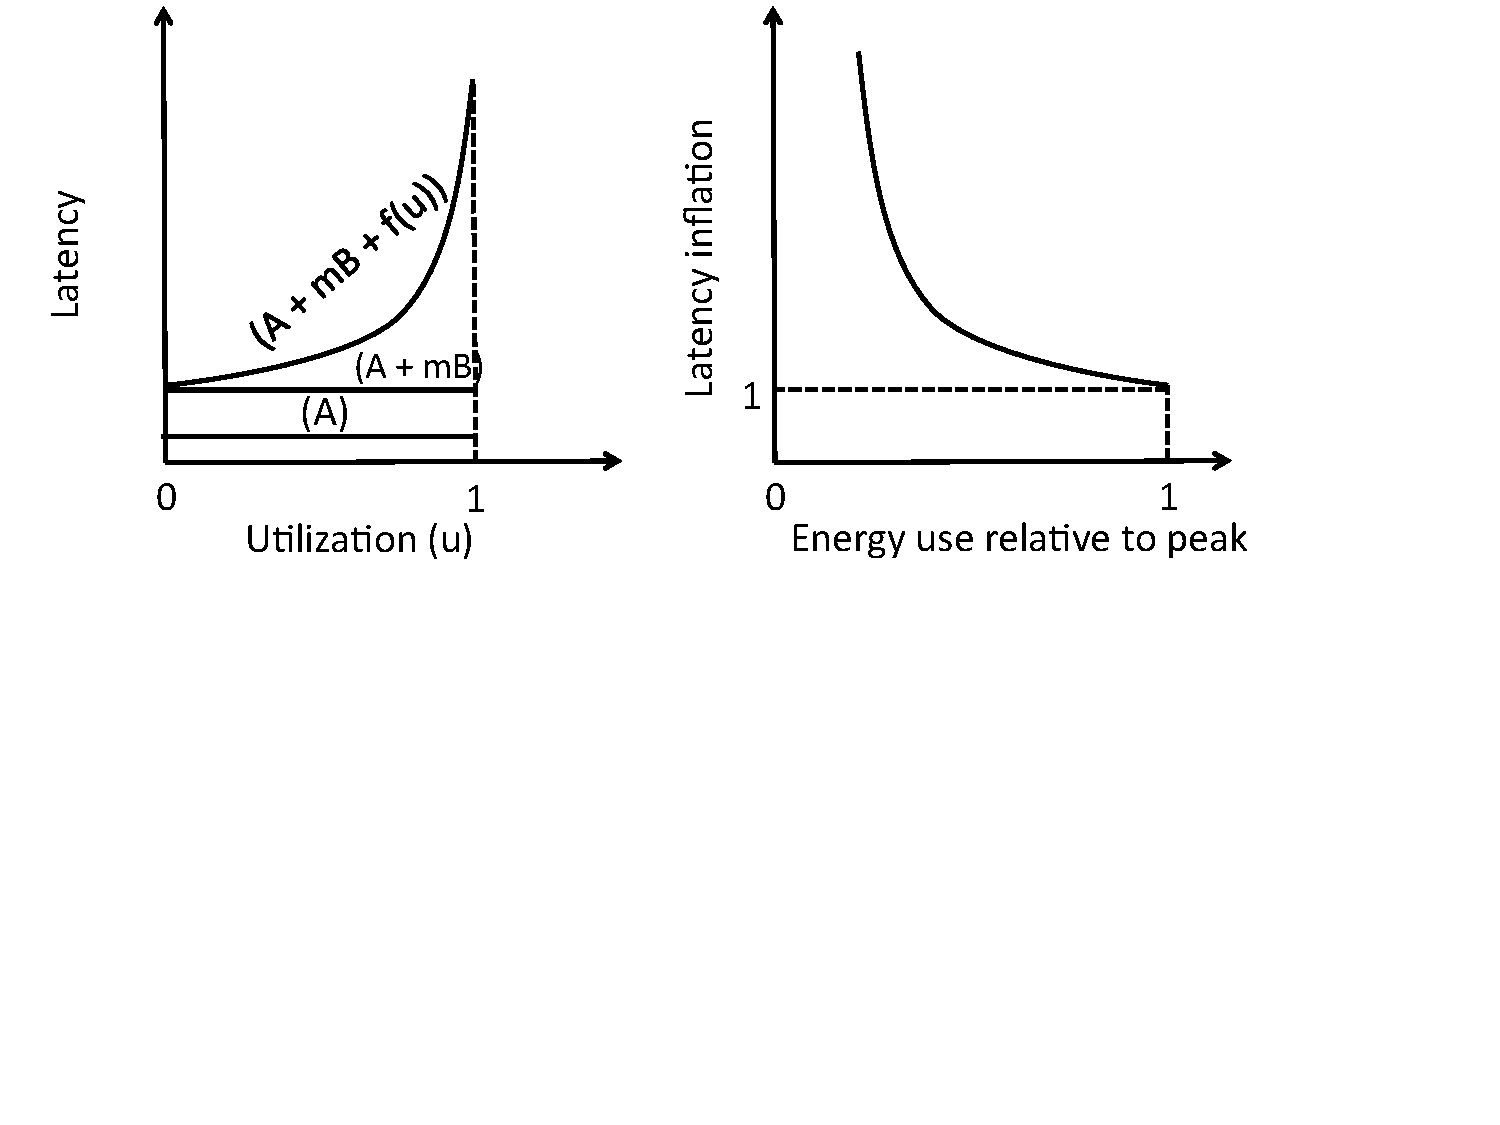
\includegraphics[scale=0.36]{figures/model.pdf}
\vspace{-1.5in}
\caption{[Left] An illustrative server utilization vs. response time curve. [Right] Corresponding energy-response time curve.}
\label{fig:model}
\end{figure}

\subsection{Single server}
\label{sec:singleserver}
Consider a single \cdc\ server serving a workload of content requests from end-users that is unchanging, i.e., the arrival rate, popularity distribution, and size distribution of content across requests is fixed. Let $m$ denote the cache miss rate at the server, i.e., the fraction of requests for which the server contacts the origin server. Assume that the power drawn by a server $p(u)$ is a linear function of its utilization $u$, or the ratio of the incoming load and the server's capacity \cite{mathew12}. In this model, an idle server's power consumption is a fraction $I$ of its peak power $P$, and the power consumed increases linearly from $IP$ to $P$ as the utilization increases from 0 to 1, i.e., $p(u) = (I + (1-I)u)P$.

The end-to-end user-perceived response time is assumed to be the sum of three components as also illustrated by the three curves in Figure \ref{fig:model} (left): (1) Mean server delay $f(u)$, assumed to be a convex, increasing function of the utilization $u$ $(0\leq u\leq1)$; (2) Server-to-origin delay $B$, which is constant but incurred only upon a cache miss; (3) Client-to-server delay $A$, a constant. Thus, the total end-to-end user-perceived delay is $f(u) + mB + A$. As shown in the figure, realistic utilization vs. server delay profile are typically somewhere in between a straight line where the delay increases linearly with the utilization and an $L$-shaped curve where the delay is zero for all values of utilization less than 1 and is infinity at 1.

\subsection{Datacenter as a single logical server}
\label{sec:multiserver}

The simplistic model above can serve as a first-order approximation of a datacenter viewed as a single logical server as follows. Suppose the datacenter consists of $N$ homogeneous servers, each identical to the one above. Suppose the total incoming load is uniformly distributed across all $N$ servers resulting in a fixed utilization $U$ at each server, which implies a power consumption of $(I+(1-I)U)P$ per server. Thus, the total power consumed is $(I+(1-I)U)PN$, and the mean response time is $f(U) + mB + A$. We have implicitly assumed here that the miss rate $m$ remains the same as above even though each server is getting a sampled transformation of the original request distribution.

What is the impact of consolidating the datacenter to $n<N$ servers on the total power consumed and user-perceived response time? To answer the first part, we observe that the utilization at each server increases by a factor $N/n$, so its power consumption would increase to $(I+(1-I)UN/n)P$. Thus, the consolidated datacenter's total power consumption is given by $(nI + (1-I)UN)P$, and the corresponding energy use relative to the peak (the x-axis in Figure  \ref{fig:model} (right)) is 
\begin{eqnarray}
\textit{benefit}  = \frac{ (nI + (1-I)UN)P}{(I+(1-I)U)PN}
\label{eq:benefit}
\end{eqnarray}

Computing the corresponding end-to-end response time with the consolidation as above is nontrivial as it requires us to account also for the increase in cache miss rates. Assuming that shutting down servers results in a proportional decrease by a factor $N/n$ in the total available storage (an assumption that is natural for clusters of commodity PCs--the more common option in practice--but not for CDCs relying on network storage), we need to compute the mean miss rate $m'$ that in general would be lower than $m$. In our numerical examples below, we derive $m'$ using a characteristic-time approximation model for an LRU cache \cite{che2002hierarchical}. 
The response time is given by $f(UN/n) + m'B + A$, and the corresponding response time 
inflation is given by 
\begin{eqnarray}
\textit{cost}  = \frac{ (f(UN/n) + mB + A)}{  (f(U) + m'B + A)}.
\label{eq:cost}
\end{eqnarray}

We make two observations based on the expression for the response time inflation above. First, the more skewed (closer to L-shaped as opposed to linear) the server's utilization vs. delay profile is, the less noticeable the impact on response time as $f(UN/n) \approx f(U)$ unless $UN/n \to 1$. Second, the more skewed (e.g., a high Zipf exponent) the popularity distribution is, the less noticeable the impact on response time as $m' \approx m$ assuming that the consolidated storage also suffices to cache the small fraction of popular objects contributing to the overwhelming portion of hits. We numerically exemplify this second insight next.
%
%\begin{figure}[t]
%\centering
%\begin{subfigure}[b]{0.23\textwidth}
%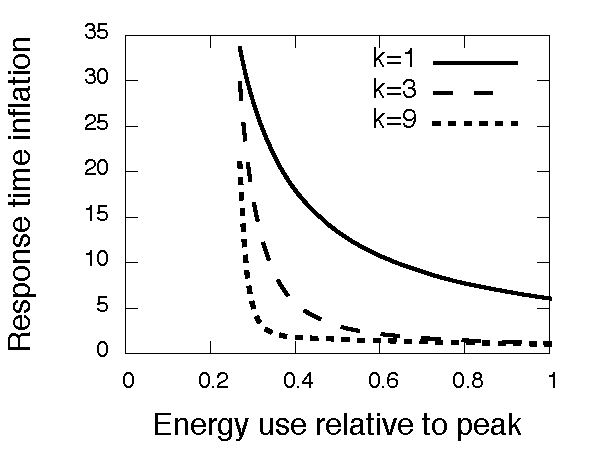
\includegraphics[scale=0.4]{graphs/vary-k.pdf}
%	\caption{}
%	\label{fig:vary-k}
%        \end{subfigure}
%\begin{subfigure}[b]{0.20\textwidth}
%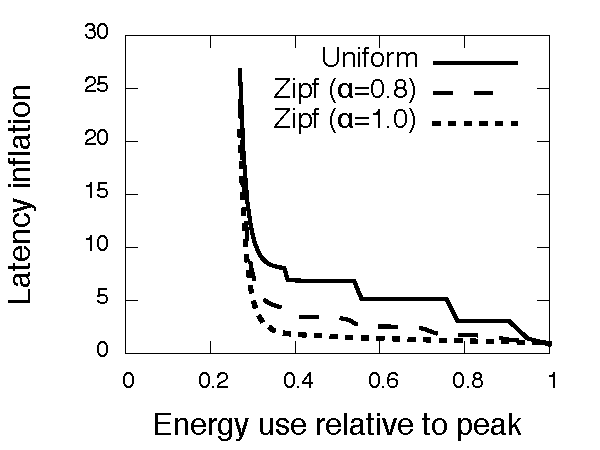
\includegraphics[scale=0.4]{graphs/vary-z.pdf}
%	\caption{}
%	\label{fig:vary-z}
%        \end{subfigure}
%\caption{Energy-response time tradeoff for (a) varying models of server delay for a Zipf workload ($\alpha$ = 1.0) and (b) workloads with varying Zipf exponents.}
%\end{figure}

\textbf{Numerical example:} We evaluate the evaluate the energy-response time tradeoff for Zipfian content popularity distributions. We assume that the server's utilization vs. delay profile is given by $f(u) = Cu^K$, $K>=1$ is a model parameter and $C$ is a constant delay. Other model parameters are as follows: each server has a capacity = 1 request/sec, total load $L$ = 15 requests/sec, latency from clients to servers $A$ = 10 ms, latency from servers to origin servers $B$ = 100 ms, server delay coefficient $C$ = 400 ms, idle power fraction $I$ = 0.5, total number of unit-sized content $M$ = 100 million, storage per server $S$ = 1 million, number of servers $N$ = 100. 

\begin{figure}[t]
\centering
    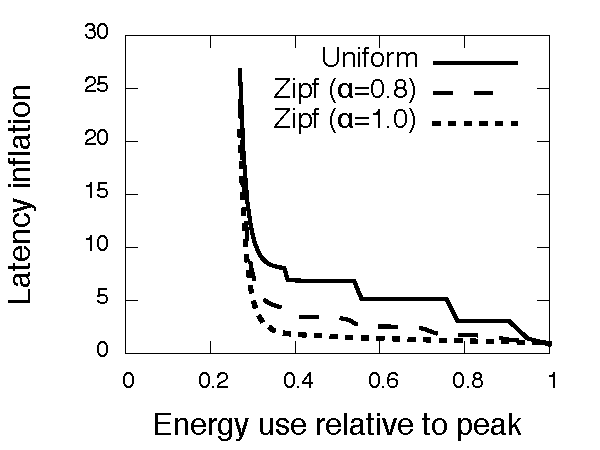
\includegraphics[scale=0.4]{graphs/vary-z.pdf}

  \caption{Energy-response time tradeoff for workloads with varying Zipf exponents.}
    \label{fig:vary-z}
\end{figure}

%\begin{figure}[t]
%\centering
%\begin{subfigure}[b]{0.23\textwidth}
%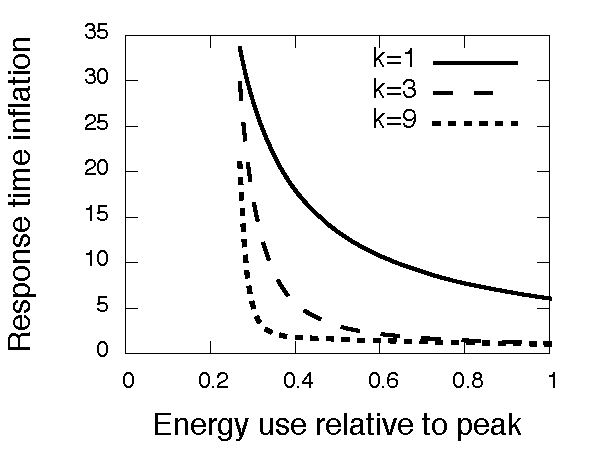
\includegraphics[scale=0.4]{graphs/vary-k.pdf}
%	\caption{}
%	\label{fig:vary-k}
%        \end{subfigure}
%\begin{subfigure}[b]{0.20\textwidth}
%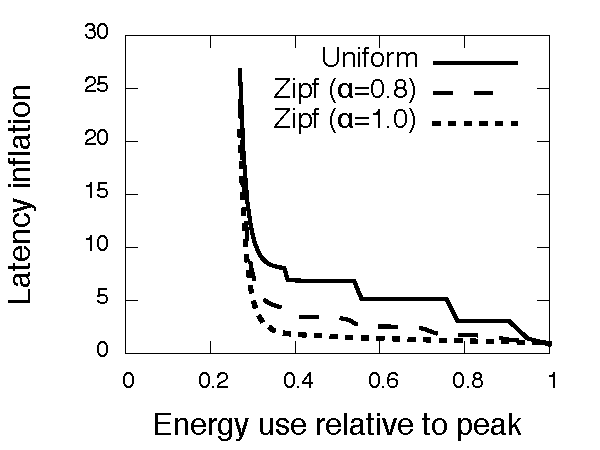
\includegraphics[scale=0.4]{graphs/vary-z.pdf}
%	\caption{}
%	\label{fig:vary-z}
%        \end{subfigure}
%\caption{Energy-response time tradeoff for (a) varying models of server delay for a Zipf workload ($\alpha$ = 1.0) and (b) workloads with varying Zipf exponents.}
%\end{figure}

%In Figure \ref{fig:vary-k} and Figure \ref{fig:vary-z}, the energy use is shown relative to the peak energy use with $N$ = 100 active servers, and response time inflation is shown relative to the least response time observed in each graph.		

%We assume that the server's utilization vs. delay profile $f(u) = Cu^K$, wherein $K>=1$ is a model parameter and $C$ is a constant delay. As $K$ increases from 1 to $\infty$, the delay profile becomes increasingly skewed. 

%In order to calculate the change in the hit rate when storage is reduced from $NS$ to $nS$, we use the following characteristic-time model \cite{che2002hierarchical}.
%\TBD{ [Equations here?]}
						
%Figure \ref{fig:vary-k} presents results for three models of server queuing delay with parameters $k$ = 1, 3 and 9; the Zipf exponent of the workload is $\alpha$ = 1.0 in all cases. In our model, the hit rates are independent of the server delay model. Therefore, the differences in response time among the curves is entirely due to a change in the server delay. We observe that the curve with $k$ = 9 achieves a significantly better energy-response time tradeoff than the curve k = 1. Further, the curve with $k$ = 9 stays nearly flat as energy use reduces by 60\% over peak. The reason is that server delays remain a small fraction of response times even at high utilization for $k$ = 9, and as a result, significant energy savings can be achieved with a small response time inflation.

Figure \ref{fig:vary-z} presents results for workloads with Zipf exponent $\alpha$ = 1.0, 0.8 and 0; $\alpha = 0$ results in a uniform distribution. The energy use is shown relative to the peak energy use with $N$ = 100 active servers, and response time inflation is shown relative to the least response time in the graph. The server  delay model parameter is $K$ = 9 for all workloads which implies that the difference in response times among them is due to a difference in  miss rates. We observe that workloads with higher Zipf exponents achieve a better energy-response time tradeoff. The reason is that a higher Zipf exponent means that most of the hits result from a small fraction of objects, so reducing the available storage only results in a small increase in miss rates. 
%A key implication is that real workloads which commonly exhibit a Zipf exponent close to 1.0 \cite{fayazbakhsh2013less} can expect to achieve a good energy vs. response time tradeoff.
	

\textbf{Summary:}
Our simple expository model suggests that the energy vs. response time tradeoff is more favorable as the skew in the server's utilization vs. delay profile increases and the skew in the content popularity distribution increases. Admittedly, this simplistic model has several critical limitations as it (1) does not consider workload dynamics, (2) assumes a perfect load balance among servers, (3) ignores the overhead of coordination between servers, and (4) implicitly assumes that the utilization vs. response time behavior and the cache size vs. miss rate behavior can be approximated by treating the \cdc\ as a single logical server of the same total capacity, ignoring the network fabric entirely. 

Thus, a natural question is what do real, achievable energy vs. response time inflation tradeoffs look like in \cdc s? 
Further, does an increase server load or an increase in cache miss rates cause a greater impact on response time? 
To answer these questions, we present the design and implementation of Shrink and evaluate the tradeoff using a real workload from a large \cdc\  in the next two sections.
%!TEX root = New.tex
\section{\shrink\ Design}

\shrink\ is a cluster manager that handles traffic engineering, load balancing and power management in CDN datacenters for maximizing energy savings with minimal effect on user-perceived performance or hardware reliability. This section provides an architectural overview of the system,  the CDN datacenter model on which \shrink's design is based, the energy,  performance, and reliability metrics which \shrink\ optimizes.


\subsection{Architectural overview}

\shrink\ is a cluster manager software which runs at the front-end load balancer. \shrink\ requires support from daemon processes running at each server for reporting content demand statistics to \shrink\ and to execute content transfer decisions sent to it. \shrink\ also requires datacenter switches to support OpenFlow in order to implement its traffic engineering decisions. 
The functionality to support powering on/off switches and servers is implemented via TBD and TBD respectively. Servers at the datacenter periodically report content demand statistics to \shrink, based on which it computes a set of load balancing, traffic engineering and content transfer decisions, and also decides which set of servers and switches to keep active in the next interval. The computed load balancing decisions are updated locally, and servers and switches are informed of the updated content transfer and traffic engineering decisions respectively. When all servers report that content transfer is complete, \shrink\ informs switches and servers to turn on/off as necessary.

\subsection{CDN datacenter model}

Table 1 lists all the model parameters. 
A CDN datacenter consists of a set of nodes $V$, which are either servers $S$ or switches $R$. The nodes are connected by a set of directed edges $E$ that represent the datacenter network links. All servers are homogenous and have a storage  $D$ and can serve traffic at a peak capacity of $B$ (in bits/sec).  Each link $e\in E$ has a capacity  $C_e$.

The set of content requested by end-users is represented by the set $K$ and the sizes of content are denoted by $S_k, k\in K$.  A demand vector $T$ specifies the demand for each content, such that the $k$-th entry of this vector $T_k$ denotes the demand for content $k\in K$.

The rest of the Internet excluding this datacenter, which includes end-users and other data centers, are modeled as virtual node $o$. The virtual node connects to the root nodes in datacenter network via virtual links which are assumed to have very high capacity. Content requested by clients are sent from servers via root nodes to this virtual node $o$. Also, any content that is unavailable within the datacenter can be fetched from the virtual node $o$ to  any server in the datacenter.

\textbf{Energy model:}  Our energy models reflects typical power usage  of switches and servers. The energy use of a switch  $i \in R$ that is turned on  $PR_i$. A switch consumes the same amount of energy independent of the rate at which it is forwarding traffic. Indeed, several  switch vendors report that their switches consume in excess of 90\% of their peak power in idle state. A server $i \in S$ consumes a fraction $f$ of its peak power $PS_i$ when idle. As server utilization increases from 0\% to 100\%, server's energy use grows linearly from $f\times PS_i$ to $PS_i$. 

%is the sum of energy consumption of the chassis  and of the line cards plugged into the chassis.  All routers have a similar chassis which consumes $R$ units of energy, the line card for link $e \in E$ uses $L_e$ energy units on routers at both ends.

%Energy consumption of a server in use in $P$ watts. At any time, only a subset of servers at a PoP are turned on at any time to reduce energy use. Total energy use of servers at a PoP is $P$ times the number of servers that are turned on.


\subsection{Problem statement}

\shrink's goal is to minimize the energy use of server and network components in a datacenter. Moreover, the system must meet following performance and reliability constraints: 
\begin{itemize}
\item
We target to provide three-nines of server availability, which is a common SLA guarantee provided by CDNs. A server is said to be available to serve a request if it has enough spare resources to start serving the request without delay.
\item
Requests that require the content to be fetched from servers outside datacenters and incur a high latency for the end-user. We seek to ensure that  the fraction of such requests increases by no more than a small percentage ($\approx 10\%$) compared to the current CDN policy of keeping entire datacenters in an always on state.
\item
Transitions between on and off states cause wear-and-tear and reduce hardware reliability. We aim to keep the frequency of on/off transitions of a server or a switch to less than once per day.
\end{itemize}

% What about fault tolerance goals?

Towards achieving above goals, \shrink\ makes following set of decisions that are formally defined below:

%The set of decisions made by \shrink\ are formally defined as follows: 
\emph{Power management:} Compute binary variables $p_i, i \in V$ to decide whether servers and switches are powered on  ($p_i = 1$) or off ($p_i = 0$).

\emph{Load balancing:} Compute variables  $l_{ks} \forall k \in K, \forall  s \in S$ such that $\sum_k l_{ks} = 1$, where $l_{ks}$ denotes the fraction of requests for content $k$ that are sent to server $s$.

\emph{Traffic engineering:} Compute routing between nodes $i,j \in V \cup \{o\}$ by deciding variables  $f_{ije} \forall i,j \in V \cup \{o\} \forall e\in E$, which denote the fraction of traffic from $i$ to $j$ that flows on link $e$.

\emph{Pre-shutdown content transfer:} Compute the set of content transfers to be done prior to shutdown of a set of servers, where a content transfer is defined by a three-tuple $(k, i, j)$, which denotes that content $k \in K$ is to be copied from server $i \in S'$, to sever $j \in S''$, where $S'$ is the set of servers being shutdown at a current stage  and $S''$  is the set of servers that will remain active post-shutdown. 

\eat{
(1) Select number of servers to keep on considering both cache hit rates and aggregate load. T is a parameter, that is empirically defined. 

(2) Select number of components that are kept active using an optimization algorithm. Coordinated server and network shutdown. Retain same components as much as possible. 

(3) Load balancing algorithm. Describe how we account for server-to-server traffic. Minimum number for fault-tolerance. Making load-balancing energy-aware. 

(4) (Content transfers?)

(5) Traffic engineering is simple.


}
\subsection{Algorithms}
\label{sec:heuristic}

With some simplifications, we have formulated the optimal strategy for the above problem as a mixed-integer program. But, we find that the optimal strategy takes tens of minutes to compute a solution even for a small-scale datacenter with few tens of nodes, and could fail to meet the three-nines availability goal in case of sudden spikes in content demand. Therefore, \shrink\ uses a set of computationally efficient heuristics to make all the above decisions which are described next. A description of the optimal strategy is presented in the Appendix \ref{sec:optimal}.

\eat{
Define a complete system which meets the above stated goals:

(1) How many servers to keep on?

(2) How to do load balancing decisions?

(3) How do decide which parts of network to keep on?

(4) How to make traffic engineering decisions?

(5) Which content to transfer before server shutdown?
}

\subsubsection{Power management}


%Power management consists of two decisions: deciding number of servers to keep on, and selecting which set of servers,  and switches to keep active. 

\shrink's power management policy is composed of two algorithms. The first algorithm decides the number of servers to be kept active, based on which the second algorithm decides which set of servers and switches are to be turned on or off. 
%Both algorithms try to maximize energy savings while reducing the number of on-off transitions.


%Our strategy is similar to those proposed by others, e.g., Matthew et al., and turn on a server immediately if average load increases over a given level, and shuts off a sever that has been unused for the past hour. The former minimizes affecting server availability, and the later reduces impact on hardware reliability.  
%The number of active servers are decided using an online algorithm whose input is a time-series of aggregate load on datacenter. A data point in this time series reflects the load in a 1-minute window and is calculated by summing the utilizations reported by all servers in that window.

*** Don't begin with Matthew et al.***

The number of active servers are decided using an online algorithm proposed by Mathew \emph{et al.}  \cite{mathew12} whose input is a time series of aggregate load on datacenter. A data point in this time series reflects the load in a one-minute window and is calculated by summing the utilizations reported by all servers in that window. The algorithm run at one-minute intervals and decides to turn servers on or off based on three values: aggregate load in the previous minute $L\_PREV$, maximum aggregate load in the previous hour $L\_MAX$, and the current number of active servers $N$. $L\_PREV$ and $L\_MAX$ are measured relative to the capacity of a single server. If $L\_PREV > \alpha N$, turn on $\lceil \frac{L\_PREV - \alpha N}{\alpha} \rceil $ more servers. if  $L\_MAX < \alpha N$, turn off $\lceil \frac{\alpha N - L\_MAX}{\alpha} \rceil$ servers. When load increases, the algorithm immediately turns more servers on to minimize the impact on server availability.  When load decreases, the algorithm waits for an hour to see if the decrease in load persists before turning servers off, a strategy which reduces the number of on-off transitions due to a spurious decrease in load.
%If the decrease in load is spurious, this strategy avoids unnecessary on-off transitions.


Algorithm \ref{algo:power} presents the pseudocode for the algorithm to select the active switches and servers based on the number of active servers N. The N active servers are chosen to be the N leftmost leaf nodes. Thereafter, the algorithm selects a subtree in the topology with following three properties: (1) Only these N nodes are the leaf nodes. (2) The sum of link capacities between nodes at successive levels is at least as much as the sum of outgoing link capacities of active servers. This property ensures that enough switches are active at each level so that  even if all servers send data at their outgoing link capacity, there are no bottleneck links. (3) 
*** don't start with Is***

****  if we use colon " : ". bullets should be compact sentences. ****

****  

*** good subtrees = (1) and (2)  *******
Is the subtree with the minimum number of nodes, which satisfies properties (1) and (2). The third property minimizes network energy use. 
This algorithm implicitly depends on the first algorithm to minimize the number of on-off transitions of a switch. This is becasue number of transitions of a switch are limited to the maximum number of transitions made by any of its leaf nodes. As the first algorithm is effective in reducing on-off transitions for  servers, this algorithm reduces them for switches.

\begin{algorithm}[h]
  \SetAlgoLined
  \SetKwInOut{Input}{input}
  \SetKwInOut{Output}{output}
\Input{ (V,E) \emph{// nodes (V) and links (E) in topology}}
\Input{ $n$ 	\emph{// number of active servers}}
\Output{$R$ 	\emph{// set of nodes that are in active state}}
S  = select $n$ leftmost leaf nodes \emph{/*S is set of servers in active state*/}\\
T = \{\} 	\emph{// traffic sent towards root by each node}\\

*** use macros instead of T, R, S etc *****

*** make it easier to read *****

\For{ $v \in V$}{
	\eIf{ $v \in S$}{
		T[v] = total outgoing link capacity of node $v$\\
		 \emph{/* server sends traffic at full capacity */}\\
		R = R $\cup$ \{v\}\\
	}{ 
		T[v] = 0
	}
}

H = height of tree topology \emph{// leaves have height 1}\\
\For{$ h \in  \{1,  .., (H - 1)\}$}{
	$V_h$ = nodes at height $h$ in left to right order\\
	\For{ $v \in V_h$}{
		P = parents of node $v$ in left to right order\\
		\For{ $p \in P$}{
			\If{ T[v] == 0}{
				\textbf{break} \emph{/* node has no traffic to send upwards */}
			}
			R = R $\cup$ \{p\}  // Parent p must be active\\
			L = link capacity of edge (v, p)\\
			traffic = min(T[v], L)\\
			T[p] += traffic\\
			T[v] -= traffic
		}
	}
}
\caption{Select active servers and switches}
\label{algo:power}			
\end{algorithm}

%We select severs and switches in the same subtree as much as possible. We select servers from left to right, and select switches which need to be active state to serve the given demand assuming servers are sending traffic at line rate. 
%As the number of transitions for server is reduced, this implies transitions for switches are also minimized.
%
%To minimize both the network and server energy, we select a subtree that has the requisite number of active servers at its leaves and is composed of the smallest number of active switches. 
%Among multiple such subtrees, we select a sub-tree which requires the minimum number of servers and switches to be turned on or off compared to the current configuration. 
%
%We illustrate the result of this selection policy for fat-tree and hierarchical topologies in Figure TBD. actually, define them

\subsubsection{Load balancing}

Our load balancing algorithms use the abstraction of a \emph{content bucket}. Content are mapped to buckets to using consistent hashing based on their name. A bucket abstraction decouples the runtime of the load-balancing algorithm with the number of content in the workload, and allows us to control the runtime by varying the number of buckets. While content buckets reduce the granularity of load-balancing decisions, in our experience, keeping the number of buckets to be two orders of magnitude higher than the number of servers, results in sufficiently fine-grained load balancing with an acceptable runtime for a data center with a thousand servers.

\shrink's algorithms operate on content demand statistics reported by every server once every minute. A server's report includes demand for every content bucket at that server since the last report.  \shrink's maintains a recent history of these demand statistics over the previous hour because decisions are made not only on the most recent window, but a recent history of these demand statistics. 

%k is fixed
%s_ik   
%s_i = \sum_k s_ik
%
%l_k = {i1: p_i1, i2: p_i2}

%Current assignments: {l_k} forall k
%Current loads: {s_i}

%In order to increase the likelihood of cache hits, the algorithm retains its load balancing rules from its previous run for many buckets as possible. Rules for some content buckets may need to be changed because of an overloaded server or a server shutdown. These buckets are considered in a random order, and new rules are decided by selecting the least loaded servers. 

%The algorithm main objective is to maximize the likelihood of cache hits. To this end, it retain rules from the previous period, and chooses a small number of buckets for each rule.

**** what is ? ****

*** can be retained, replace by "feasible", define what makes something feasible ****

Algorithm \ref{algo:lb} describes pseudocode for \shrink's load balancing. 
**** load balancing rule, define what a rule is  *** 
The algorithm runs once every minute and outputs a load balancing rule for each content bucket, which decides the servers that will serve its requests and the ratios in which requests will be distributed among those servers. 
***The algorithm maintains a variable to track the load assigned to each server while computing rules. *** 
The algorithm makes two passes over the set of content buckets. 
****Too long a sentence: In the first pass, a content bucket's previous load balancing rule is retained and the load assigned to servers is updated based on the bucket's demand, if all servers used by that rule are active and when this content bucket's demand is added on to them, their assigned load remains within the threshold. ****
The first pass scans buckets  in an increasing order of demand to maximize the number of load balancing rules that can retain from the previous run, which in turn increases the likelihood of cache hits. 

The second pass creates new rules for buckets *** whose previous rule is not retained.*** For each bucket, all its demand is assigned to the least loaded server. If assigning all the demand for a bucket to this server would increase its load above threshold $\alpha$, then only as much demand is assigned to the server as would keep its load below the threshold; the remaining demand is then assigned to the next least loaded server. In this manner, as many servers are selected as necessary to serve this bucket demand. The proportion in which demands assigned to those servers  determines the probabilities assigned to servers in the new load balancing rule.

****** correct spelling ******

****** make text more readable,  ******

********* remove primes' *********

********* one "input:", one "output:" *********
%Objectives: retains assignments to maximize reuse.
%(1) two-passes over the set of content buckets:
%(2) first: retain the set of buckets
%(3) second: remap unnecessary buckets

\begin{algorithm}[htbp]
  \SetAlgoLined
  \SetKwInOut{Input}{input}
  \SetKwInOut{Output}{output}
  \Input{S = \{$s_1$, ...  \} \emph{// set of active servers}}
%\noindent content = \{$c_1$, ...  \}\\
  \Input{D = \{($c_1, d_1$),  ...  \}}
\noindent \emph{/* $d_i$ is demand for content $c_i$. $d_i$ is ratio of actual demand (in bits/sec) to  capacity of one server (in bits/sec) */}\\
\Input{LBPrev = \{($c_1$, $rule_1$), .. \} }
\noindent \emph{/* $rule_i$ is previous LB rule for content $c_i$. $rule_i = \{(s_1, p_1), ...\}$ such that server $s_i$ receives a request with probability $p_i > 0$. */}\\
\Input{$\alpha$ \emph{// threshold server load. $0 < \alpha < 1$}}
  \Output{LBNew \emph{// new set of LB rules}}
  LBNew = \{\}\\
loads = \{\} \emph{// load assigned to each active server} \\

\For{$s_i$  in S}{loads[$s_i$] = 0 \emph{// initialize load  to zero}\\
}
\For{$(c_i, d_i)$  in D sorted by increasing $d_i$ } {
prevRule = LBPrev[$c_i$] \emph{// previous rule for $c_i$}\\
$S'_k$ = set of servers in prevRule\\
\If{$S'_k \not\subset S$}{ 
	\textbf{continue} \emph{/* all servers are not active, change LB rule */}
}
flag = True\\
\For{$s_j \in S'_k$}{
$p_j$ = probability of $s_j$ receiving request \\
\If{loads[$s_j$] $+$ $d_i p_j >  \alpha$}{
flag = False \emph{/* demand exceeded  server load threshold, change LB rule */}\\
}
}
\If{flag}{LBNew[$c_i$] = prevRule \emph{// copy old rule}
}
}
\For{ $(c_k, d_k)$ in D sorted by decreasing  $d_k$}{
	\If{ $c_k  \notin LBNew$}{
		newRule = \{\}\\
		\For {$(s_j, l_j) \in loads$ sorted by increasing $l_j$}{
			$p_j$ = min($1 - l_j$, $d_j$)\\
			newRule[$s_j$] = $p_j$\\
			$d_k = d_k - p_j$\\
			\If{$d_k == 0$}{break}
		}
		LBnew[$c_k$] = newRule\\
}
}
  \caption{Compute load balancing (LB) rules}
\label{algo:lb}
\end{algorithm}


%
%\IncMargin{1em}
%\begin{algorithm}
%  \SetKwData{Left}{left}\SetKwData{This}{this}\SetKwData{Up}{up}
%  \SetKwFunction{Union}{Union}\SetKwFunction{FindCompress}{FindCompress}
%  \SetKwInOut{Input}{input}\SetKwInOut{Output}{output}
%  \Input{A bitmap $Im$ of size $w\times l$}
%  \Output{A partition of the bitmap}
%  \BlankLine
%  \emph{special treatment of the first line}\;
%  \For{$i\leftarrow 2$ \KwTo $l$}{
%    \emph{special treatment of the first element of line $i$}\;
%    \For{$j\leftarrow 2$ \KwTo $w$}{\label{forins}
%      \Left$\leftarrow$ \FindCompress{$Im[i,j-1]$}\;
%      \Up$\leftarrow$ \FindCompress{$Im[i-1,]$}\;
%      \This$\leftarrow$ \FindCompress{$Im[i,j]$}\;
%      \If(\tcp*[h]{O(\Left,\This)==1}){\Left compatible with \This}{\label{lt}
%        \lIf{\Left $<$ \This}{\Union{\Left,\This}}\;
%        \lElse{\Union{\This,\Left}\;}
%      }
%      \If(\tcp*[f]{O(\Up,\This)==1}){\Up compatible with \This}{\label{ut}
%        \lIf{\Up $<$ \This}{\Union{\Up,\This}}\;
%        \tcp{\This is put under \Up to keep tree as flat as possible}\label{cmt}
%        \lElse{\Union{\This,\Up}}\tcp*[r]{\This linked to \Up}\label{lelse}
%} }
%    \lForEach{element $e$ of the line $i$}{\FindCompress{p}}
%  }
%  \caption{disjoint decomposition}\label{algo_disjdecomp}
%\end{algorithm}\DecMargin{1em}
\subsubsection{Traffic engineering}

Inverse cap with ECMP is sufficient to use available path diversity in the best-possible manner.


\subsubsection{Pre-shutdown content transfers}

Select content available in past time window, and transfer it to other servers.

\subsubsection{Failure handling}

How does \shrink\ handle server failures? 

(1) A content bucket is placed on at least two servers. If one of the servers for a content bucket fails, other server handles all requests until next load balancing event. There is a brief period of (one epoch) of sub-optimal load balancing.

(2) Load balancing recomputes rules in the next run to balance load among servers, and starting new servers if necessary.

How does \shrink\ handle switch failures?

(1) Need to add the constraint that no single switch failure makes both servers responsible for a content bucket unavailable.


%!TEX root = shrink.tex
\section{Experimental Evaluation}
\label{sec:shrink-eval}
\newcommand{\peakS}{Peak-S}
\newcommand{\peakSN}{Peak-SN}
\newcommand{\randSN}{Rand-SN}

Our evaluation has two main goals: (1) Comparing the network energy use of \shrink\ against a network-unaware server consolidation scheme (Section \ref{sec:net-compare}). (2) Quantifying the energy-response time tradeoff achieved by \shrink\ and compare it to the ideal energy response time tradeoff achievable (Section \ref{sec:quantify}).

\begin{figure}[t]
        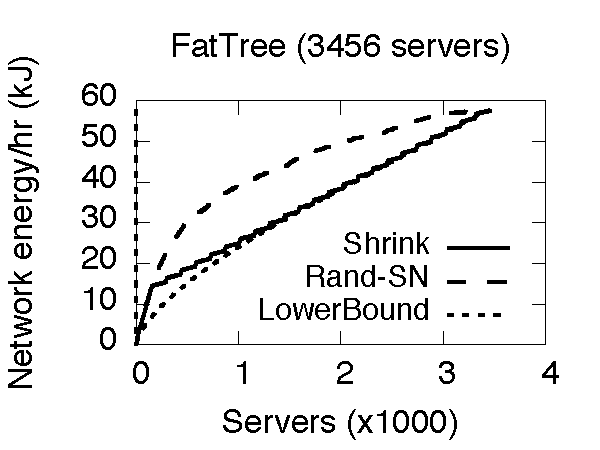
\includegraphics[scale=0.4]{graphs/final/fattree-24.pdf}
                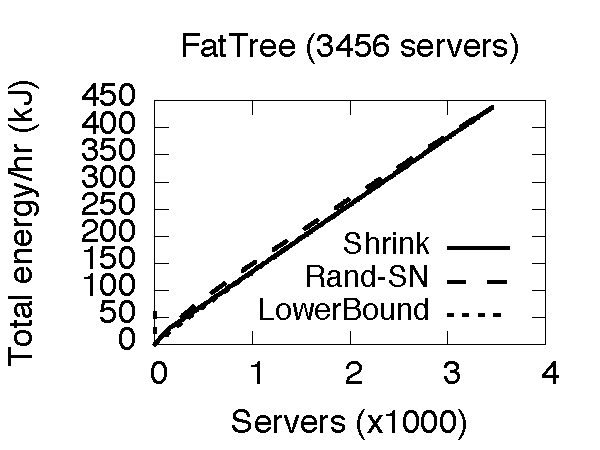
\includegraphics[scale=0.4]{graphs/final/fattree-24-total.pdf}
                        \centering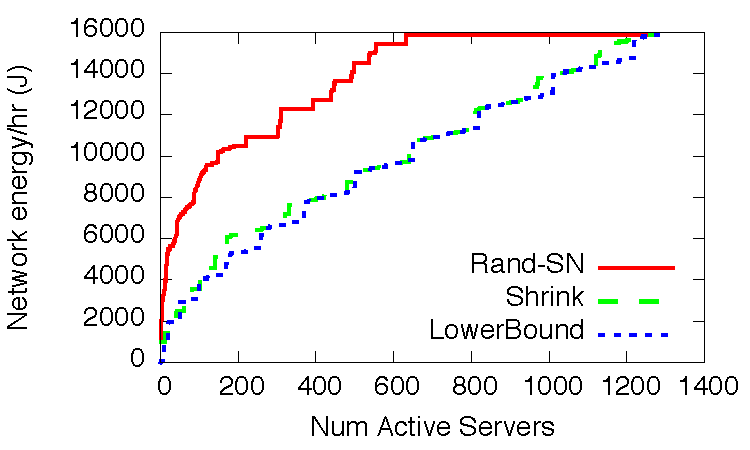
\includegraphics[scale=0.4]{graphs/final/vl2.pdf}
                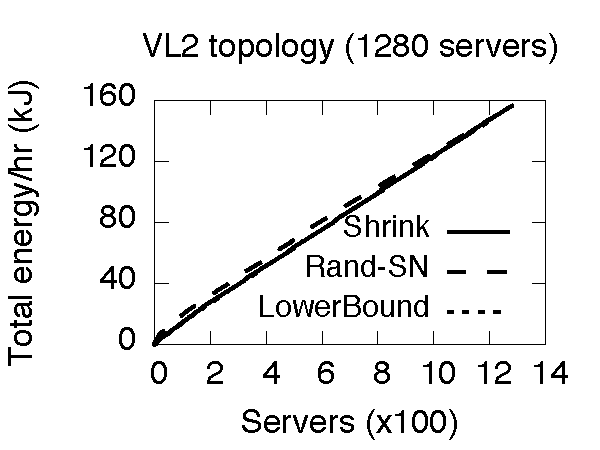
\includegraphics[scale=0.4]{graphs/final/vl2-total.pdf}
\caption{[Numerical computation] \shrink's network energy use is lower than a network-unaware server consolidation scheme \randSN\ by 38\% on FatTree and 42\% on VL2 when one-fourth of the servers are active in each topology.}
\label{fig:fattree}
\end{figure}

\subsection{Comparing network energy use}
\label{sec:net-compare}

\textbf{Schemes compared:}   (1) \emph{\randSN:} \randSN\ selects the set of active servers randomly; it uses the same network consolidation scheme as \shrink.  \randSN\ is used to evaluate the benefit of network-aware server consolidation in \shrink. (2) \emph{LowerBound:} We define lower bounds on the network energy use for a given number of active servers on the FatTree and the VL2 topologies. Our computation of LowerBound for FatTree and VL2 is described in Appendix \ref{sec:netlb}. \randSN\ and LowerBound provide the same per-server bandwidth guarantee to external hosts as \shrink\ does.

\textbf{Topologies:}  We simulate two network topologies:  a 3456-server FatTree topology made of 24-port switches (Cisco Nexus 2224P, 80 Watt, 720 count) \cite{cisco-dc-switches} consuming 80 Watt per switch, and a 1280-server VL2 topology made of 24-port ToR switches (Cisco Nexus 2224P, 80 W, 64 count) \cite{cisco-dc-switches} and 16-port 10 Gigabit core or aggregation switches (Cisco Catalyst 6500, 480 W, 24 count) \cite{catalyst-6500}. We assume all active servers have identical power use (Acer Altos T350 F2, 130W at 60\% utilization \cite{spec}).

\textbf{Results:}  Figure \ref{fig:fattree} presents our results.
%compares \shrink\ against \randSN\ and the lower bounds on network energy use for the simulated topologies.
The relative difference between \shrink\ and \randSN\ reduces as the number of active servers increases. 
When 25\% and 50\% of servers are active, \shrink's network energy use is lower than \randSN\ by 38\% and 26\% respectively on FatTree and 42\% and 35\% respectively on VL2. 
When 25\% and 50\% of servers are active, \shrink's network energy use higher than LowerBound by 9\% and 2\% respectively on FatTree and by 13\% and 7\% respectively on VL2. 
These findings show that \shrink's network-aware server consolidation reduces the network energy use over network-unaware server consolidation schemes and gives network energy savings close to the lower bound.
When 25\% and 50\% of servers are active, \shrink's \emph{total} energy use is lower than \randSN\ by 9\% and 5\% respectively on FatTree and 10\% and 7\% respectively on VL2. 
Thus, \shrink's network-aware server consolidation is effective in reducing aggregate \cdc\ energy use as well. 

%Considering scenarios where at least one-fifth of servers are active, \shrink\ uses up to 39\% less network energy on FatTree and up to 45\% less energy on VL2 compared to the network-unaware scheme, \randSN. 


\begin{figure*}
        \centering
        \subfigure[Mean]{\label{fig:pe-mean}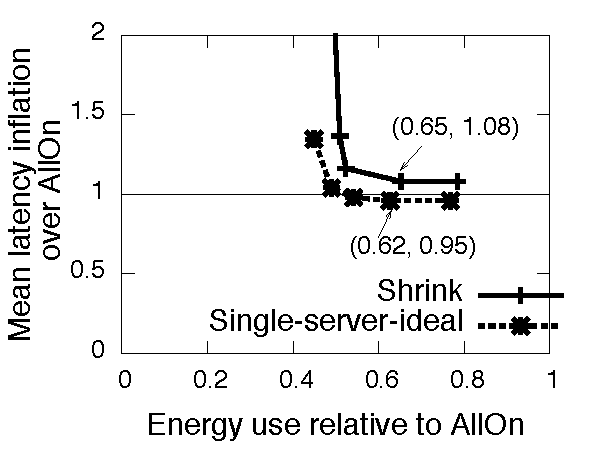
\includegraphics[scale=0.47]{graphs/final/mean.pdf}}
         \subfigure[95-th percentile]{\label{fig:pe-95}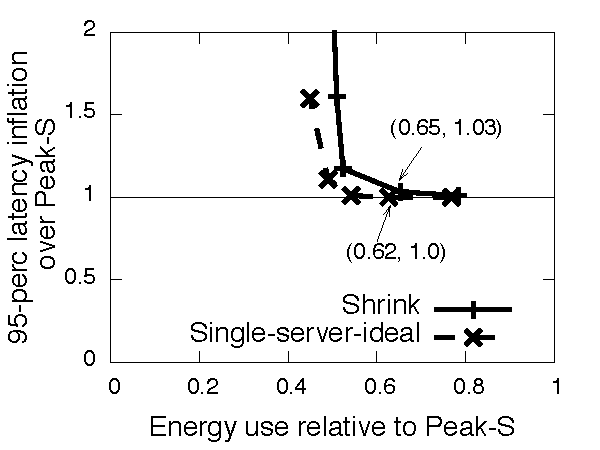
\includegraphics[scale=0.47]{graphs/final/perc95.pdf}}	       \subfigure[99-th percentile]{\label{fig:pe-99}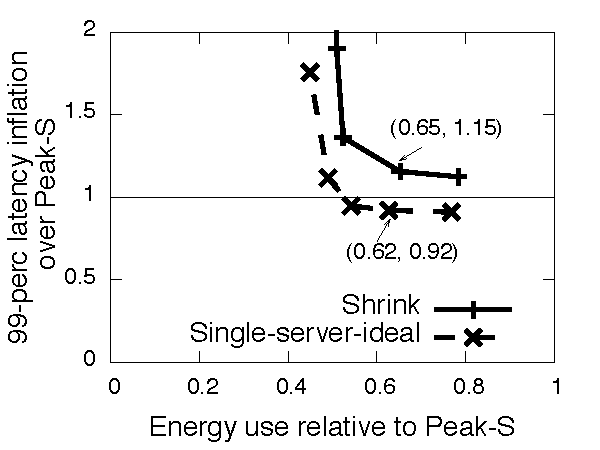
\includegraphics[scale=0.47]{graphs/final/perc99.pdf}}	
        \caption{Server consolidation (Section \ref{sec:ec2}):  \shrink's reduces energy over \peakS\ with a small response time inflation. In Figure \ref{fig:pe-mean}, \shrink's energy use is 0.65$\times$ of \peakS\ and its mean response time is 1.08$\times$ of \peakS; Single-server-ideal's energy use is 0.62$\times$  of \peakS\ and its mean response time is 0.95$\times$ of \peakS.}
        \label{fig:pe}
\end{figure*}

\subsection{Quantifying energy-response time tradeoff}
\label{sec:quantify}
\vspace{-0.1in}
\subsubsection{Experiment setup}
\label{sec:setup}
\textbf{Akamai dataset:} Our evaluation uses content access traces from an Akamai datacenter. The traces include all requests received at a datacenter with 24 servers for a week in December 2013. We restricted our data collection to a small datacenter as we did not have the resources to experiment with traces from a significantly larger datacenter. Our anonymized traces include several major types of traffic observed in a CDN such as video, social media and other web traffic. Each anonymized log entry includes among other fields, the request timestamp, content URL, size of requested content, actual number of bytes sent and IP address of the user. Overall, the traces contain more than 2 billion requests generating nearly 200 TB of network traffic.

\textbf{Testbeds:} We use prototype-based experiments (on EC2 and Emulab) and trace-based experiments. Our experiment on EC2 evaluates the energy-response time tradeoff due to server-only consolidation. As we do not have control over network topology on EC2, we use Emulab to evaluate the response time inflation due to both server and network consolidation. Finally, we conduct larger-scale trace-based experiments on a simulator.






%\begin{figure}[t]
%        \centering
%        \begin{subfigure}{0.24\textwidth}
%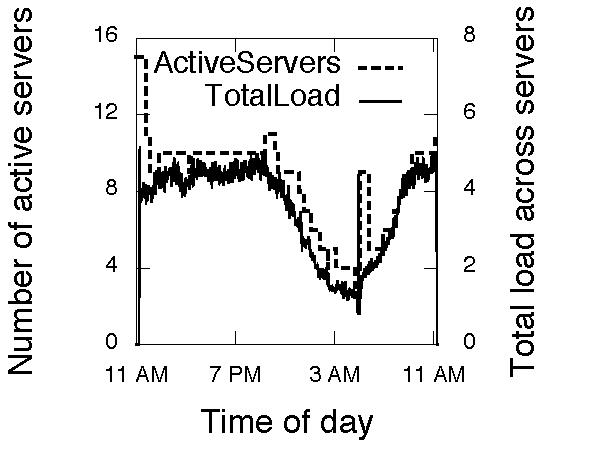
\includegraphics[scale=0.4]{graphs/final/num-servers.pdf}
%\caption{}
%\label{fig:num-servers}
%        \end{subfigure}
%        \begin{subfigure}{0.24\textwidth}
%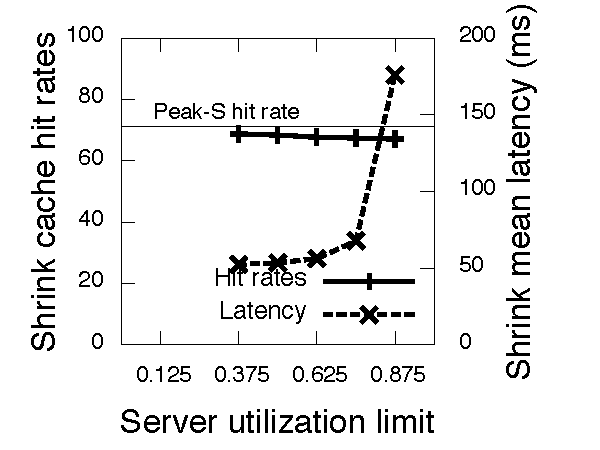
\includegraphics[scale=0.4]{graphs/final/hit-rate.pdf}
%\caption{}
%\label{fig:hitrate}
%        \end{subfigure}
%        \caption{[EC2] \shrink\ adapts the number of active servers based on \cdc\  load to reduce energy over \peakS. Cache hit rates and mean response time for \shrink\ and \peakS.}
%\end{figure}


%\centering
%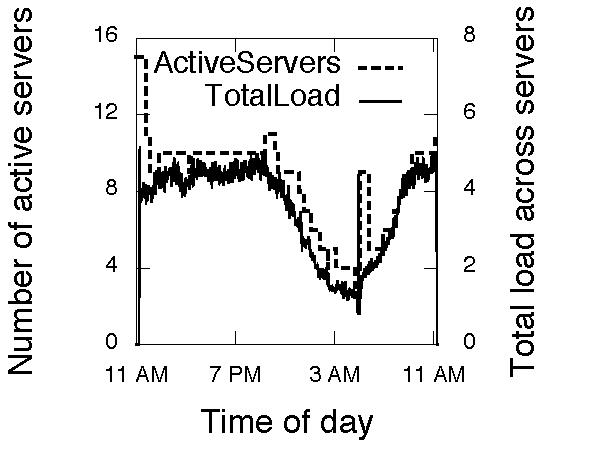
\includegraphics[scale=0.6]{graphs/final/num-servers.pdf}
%\caption{[EC2] \shrink\ adapts the number of active servers based on \cdc\  load to reduce energy over \peakS.}
%\label{fig:num-servers}
%\end{minipage}
%\hspace{0.5cm}
%\begin{minipage}{0.3\textwidth}
%\centering
%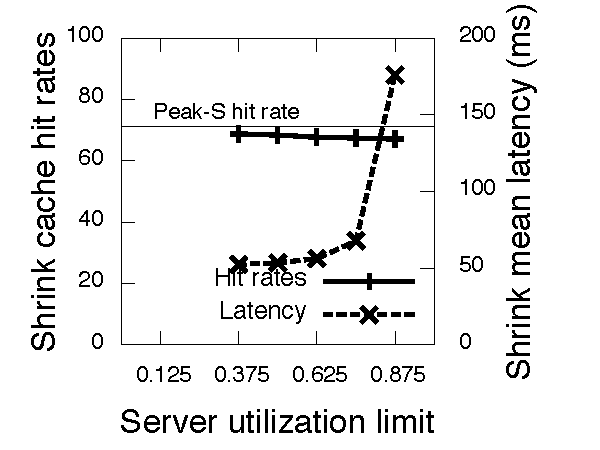
\includegraphics[scale=0.6]{graphs/final/hit-rate.pdf}
%\caption{[EC2] Cache hit rates and mean response time for \shrink\ and \peakS.}
%\label{fig:hitrate}
%\end{minipage}
%\hspace{0.5cm}
%\begin{minipage}{0.3\textwidth}
%\centering
%	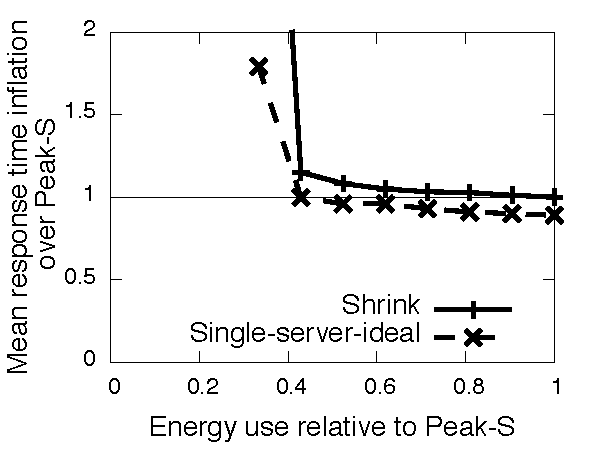
\includegraphics[scale=0.55]{graphs/final/emulab-mean.pdf}
%	\caption{[Emulab] Network and server consolidation: For an 15\% increase in mean response time, \shrink\ reduces energy use by 57\% over \peakS.}
%	\label{fig:pe-mean-2}
%
%\end{minipage}
%\end{figure*}

%
%\begin{figure*}
%\begin{minipage}{0.3\textwidth}
%\centering
%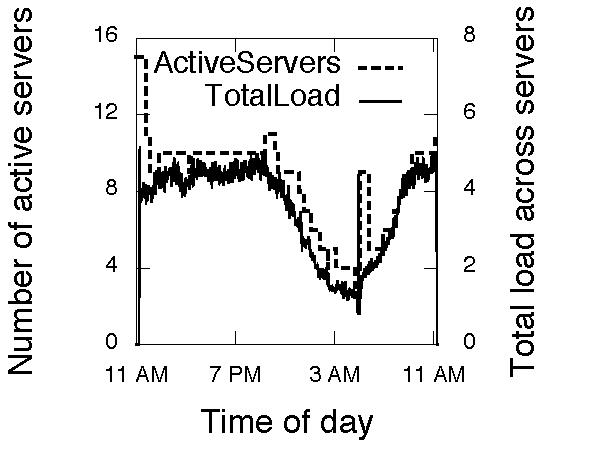
\includegraphics[scale=0.6]{graphs/final/num-servers.pdf}
%\caption{[EC2] \shrink\ adapts the number of active servers based on \cdc\  load to reduce energy over \peakS.}
%\label{fig:num-servers}
%\end{minipage}
%\hspace{0.5cm}
%\begin{minipage}{0.3\textwidth}
%\centering
%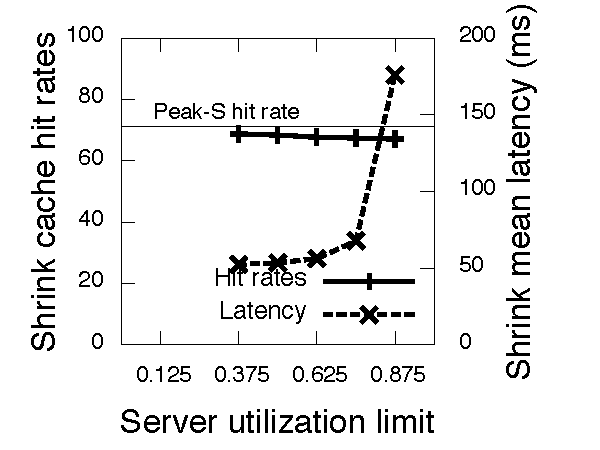
\includegraphics[scale=0.6]{graphs/final/hit-rate.pdf}
%\caption{[EC2] Cache hit rates and mean response time for \shrink\ and \peakS.}
%\label{fig:hitrate}
%\end{minipage}
%\hspace{0.5cm}
%\begin{minipage}{0.3\textwidth}
%\centering
%	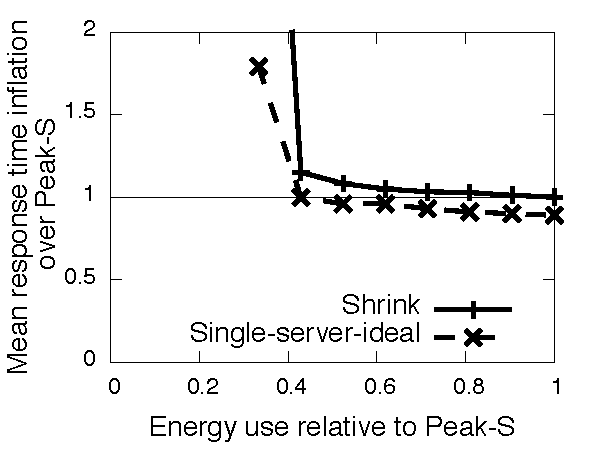
\includegraphics[scale=0.55]{graphs/final/emulab-mean.pdf}
%	\caption{[Emulab] Network and server consolidation: For an 15\% increase in mean response time, \shrink\ reduces energy use by 57\% over \peakS.}
%	\label{fig:pe-mean-2}
%
%\end{minipage}
%\end{figure*}


\textbf{Schemes compared:} We compare \shrink\ against \emph{\peakS} and \emph{Single-server-ideal}. \peakS\ represents a baseline in which a \cdc\ operator does not use consolidation to reduce energy use, i.e., it keeps all servers and switches active.

Single-server-ideal is a computation of the ideal energy-response time curve, unachievable by any real system. The points on this curve are obtained by varying the utilization $u$ up to which any server can be loaded. For a given $u$, the response time of Single-server-ideal for a given metric is equal to the measured load-vs.-response time curve of a single server for the same metric at the same utilization. For the same utilization $u$, any distributed system will have a higher response time because workload dynamics, load imbalance and non-steady state cache behavior; these factors are ignored by Single-server-ideal. Our single server measurements are done with a representative workload in the respective experimental environment, EC2 or Emulab, with emulated client-to-server delay and server-to-origin delay. 

%taken to be response of a single server in steady-state at the same utilization. In doing so, we assume that the response time of the entire \cdc\ at a given average utilization is the same as that of a single server  at the same utilization. 

For Single-server-ideal, we compute the set of servers and switches in each time interval that minimizes the total energy use as follows. Based on four inputs -- $u$, the total load in each time interval, the number of server transitions allowed, and the power model of each server --, we use a dynamic programming algorithm to compute the total energy use of servers and the number of active servers in each time interval. The number of transitions is equal to one on-off server transition/server/day or the same number of transitions as \shrink\ in that experiment, whichever is higher. The ideal network energy use for the tree topology we experiment with (Section \ref{sec:emulab}) is computed based on the number of active servers in each time interval. The set of active servers are selected in a left-to-right order; for each active server, we select the switches on the path to the root. The set of switches selected across all active servers is the set that optimizes network energy use.

%Single-server-ideal is a computation of the ideal energy-response time curve. In our computation, we assume that the utilization-vs.-response time curve for the entire \cdc\  is the same as that of a single server system at the same utilization, which is in steady state and has an infinite cache. 
%The response time of Single-server-ideal is \emph{ideal}, as discussed in Section \ref{sec:analysis}. For our computation, we obtained the utilization-vs.-response time curve for a single server by measuring response time metrics at varying request rates and using a cache size large enough so that steady state response times can be measured without exhausting the cache.
%
%The energy calculation for Single-server-ideal assumes prior knowledge of the total load in each time interval and the number of server transitions allowed. We allow Single-server-ideal to make one on-off server transition/server/day or the same number of transitions as \shrink\ in that experiment, whichever is higher. Based on these inputs, we use a dynamic programming algorithm \cite{mathew12} to compute the total energy use of servers and the number of active servers in each time interval.  The network energy use for the tree topology we experiment with (Section \ref{sec:emulab}) is computed as follows: For each active server, we select the switches on the path to the root. The set of switches selected across all active servers is the set that optimizes network energy use.



\subsubsection{Prototype-based experiments: server consolidation}
\label{sec:ec2}
\vspace{-0.1in}
This experiment quantifies the energy-response time tradeoff due to server consolidation on EC2. Our EC2 testbed consists of 15 servers, 15 clients and 4 origin servers running on independent m3.xlarge instances (4 core, 15 GB RAM, 40 GB$\times$2 SSD), all in the same datacenter. Our origin server is a trivial Apache Tomcat application that dynamically generates the requested content. We emulate a 60 ms RTT between origin servers and \cdc's servers, and a 10 ms RTT between client and server machines. We configured each server to use an 8 GB memory cache and a 30 GB cache on each SSD. 

Our workload consists of a 24-hour duration of the trace.  We selected one-eighth of the content randomly from the trace but sped up the trace by 8$\times$ to send those requests over a 3-hour duration. Thus, we  maintain approximately the same load on the servers. We use a short pre-shutdown wait interval $W =$ 10 min for \shrink\ because our workload is a sped up by $8\times$.

%
We calculate the energy savings relative to \peakS\ as per Equation \ref{eq:benefit}; the ratio of the idle to peak energy use of servers, $I$ equals 0.5 \cite{barroso2007case}. \peakS\ uses 15 servers in this experiment. We have conservatively chosen the number of servers in \peakS\ to be much less than the number of servers in the Akamai datacenter itself so as not to overestimate the energy savings. 



We evaluate \shrink\ in terms of three response time metrics --  mean, 95-percentile, 99-percentile. 
To provide a utilization-vs.-response time curve $F(.)$ to \shrink\ for each metric, we take the first approach discussed in Section \ref{sec:utilization-vs-responsetime}. The function $F(.)$ for each metric is equal to the measured utilization vs. response time curve of a single server with an inefficiency factor $\rho = 0.2$.  Based on $F(.)$ for each metric, we specify response times $F(u)$ to \shrink\ for values of $u$ from 0.375 to 0.875 at intervals of 0.125 across different runs. 

%, which is much less than the number of servers in the Akamai datacenter itself. we have made this choice not to overstate the energy savings.


Figure \ref{fig:pe} compares the response time and the energy use of \shrink\ relative to \peakS\ for the mean, the 95-th percentile and the 99-th percentile of response times. \shrink\ reduces energy use by 35\% over \peakS\ while inflating the mean, the 95-th percentile and the 99-th percentile by 8\%, 3\% and 15\% respectively. 
To explain the difference between \peakS\ and \shrink, consider Figure \ref{fig:ec2-other} (left)  which shows the aggregate load and the number of servers from one of the runs of the system. \shrink\  adapts the number of active servers based on load in the system keeping only 3 servers active when the load is the lowest, but \peakS\ always keeps 15 servers active and hence has a higher energy use. This result implies that an operator for which these inflations are tolerable, e.g., they do not cause an SLA violation, can achieve the corresponding energy savings as well. 




%Single-server-ideal does achieve a better energy-response time tradeoff than \shrink.  First, the energy-response time curve for Single-server-ideal is computed assuming that the response time for a given server utilization limit is equal to the response time of a single server in steady state at the same utilization. The response time for any real system, including \shrink, will be higher due to several reasons such as imperfect load balancing and non-steady state cache behavior. 




Does  an increase server load or a decrease in cache hit rates cause a greater impact on \shrink's response time over \peakS? 
In Figure \ref{fig:ec2-other} (right) the x-axis shows the server utilization limit $U$ computed by \shrink's consolidation algorithm (Section \ref{sec:serverconsolidation}) and y-axes show corresponding the  hit rates and the mean response time of \shrink. \shrink's  hit rates are lower than \peakS\ but the decrease is less than 7\% across all utilizations. 
Thus, the response time inflation due to a decrease in hit rates is likely to be small. A small reduction in hit rates is not surprising given that the Zipf exponent for the Akamai trace is 0.8 as per our calculations, and our model in Section \ref{sec:analysis} has suggested that  consolidation reduces hit rates by a small fraction for for real workloads with a high skew in content popularity.  We find that mean response times increase sharply at  a high server utilization limit, e.g. $U=0.875$, which is likely due to an increase in server load. To summarize, there is a small response time inflation due to a decrease in hit rates but severe inflation occurs at high server utilization limits, and is likely due to an increase in server  load.


Comparing \shrink\ with Single-server-ideal, in Figure \ref{fig:pe-mean}, \shrink's energy use is 0.65$\times$ of \peakS\ and its mean response time is 1.08$\times$ of \peakS; Single-server-ideal's energy use is 0.62$\times$  of \peakS\ and its mean response time is 0.95$\times$ of \peakS.  
There are two reasons that explain the gap between \shrink\ and Single-server-ideal. First, Single-server-ideal ignores several factors that increase response time of any distributed system such as workload dynamics, load imbalance and non-steady state cache behavior. Second, \shrink\ waits for the pre-shutdown wait interval to see if a decrease in load persists before turning servers off. But, in our calculation, Single-server-ideal knows the load for the entire experiment beforehand and hence it can shutdown servers sooner than \shrink\ and save more energy.

%An implication of our findings is that a simple random load balancing policy effectively avoids load hotspots and ensures only a small decrease in cache hit rates even as energy optimization schemes vary the number of active servers in a \cdc.
\begin{figure}
\centering
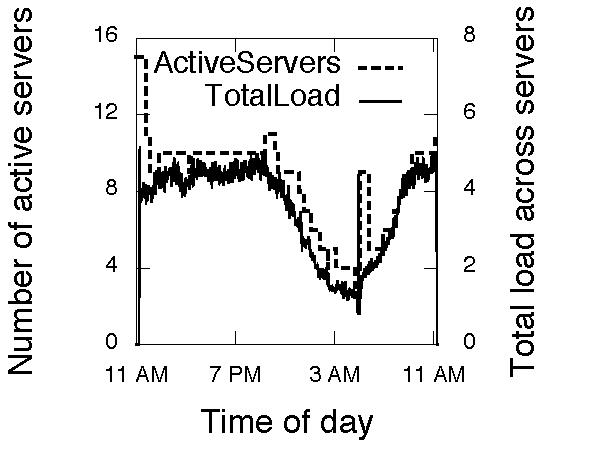
\includegraphics[scale=0.4]{graphs/final/num-servers.pdf}
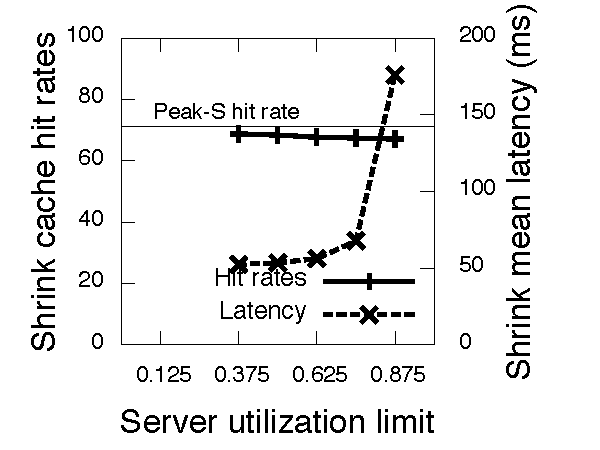
\includegraphics[scale=0.4]{graphs/final/hit-rate.pdf}
\caption{Server consolidation (Section \ref{sec:ec2}): [Left] \shrink\ adapts the number of active servers based on \cdc\  load to reduce energy over \peakS. [Right] Cache hit rates and mean response time for \shrink\ and \peakS.}
\label{fig:ec2-other}
\end{figure}

\subsubsection{Prototype-based experiments: server \& network consolidation}
\label{sec:emulab}

\begin{figure}
	\centering
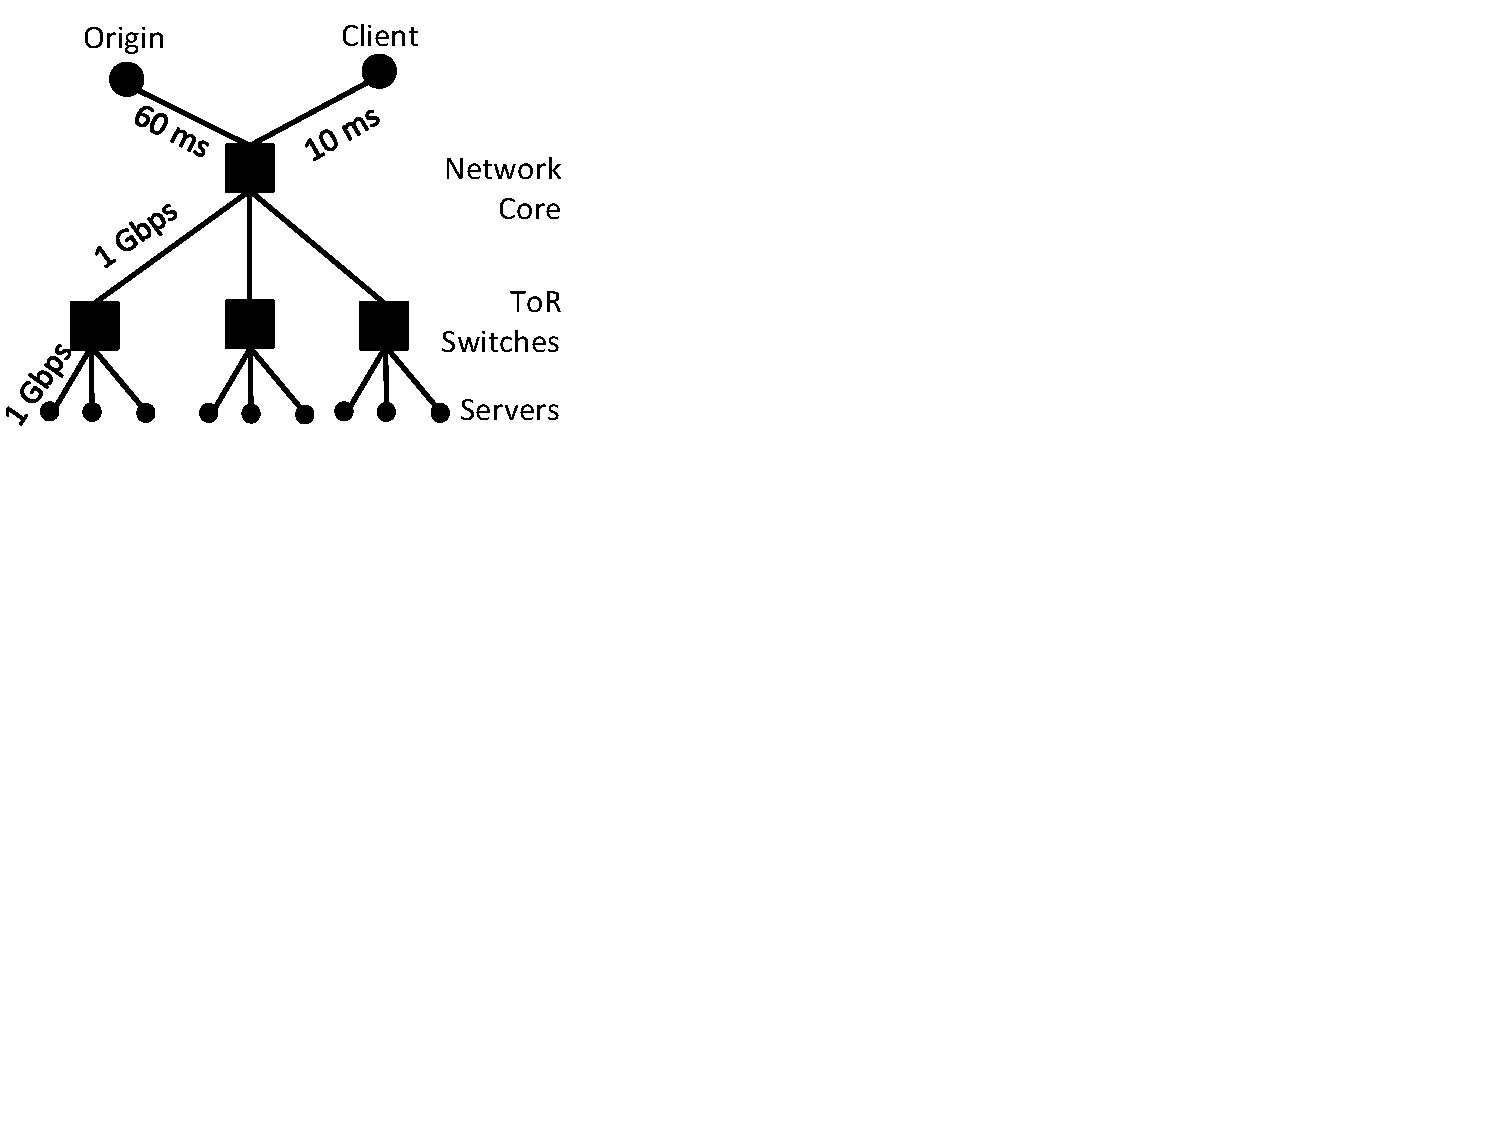
\includegraphics[scale=0.35]{figures/emulab-topo.pdf}
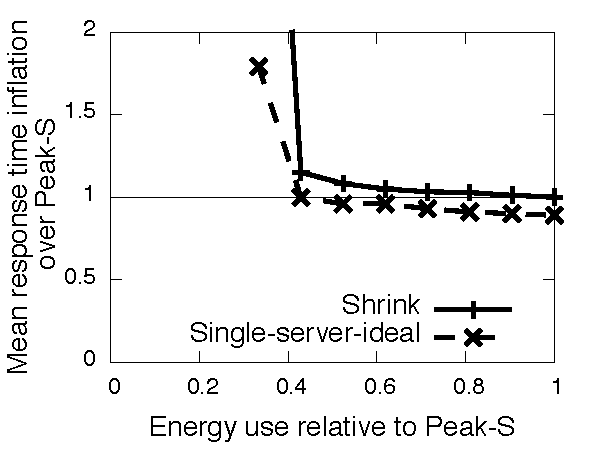
\includegraphics[scale=0.5]{graphs/final/emulab-mean.pdf}
\caption{Network and server consolidation (Section \ref{sec:emulab}): [Left] Emulab topology for the experiment. [Right] Compared to \peakS, \shrink\ has a 15\% higher response time but a 57\% lower energy use.}
\label{fig:emulab}
\end{figure}

We use Emulab to evaluate the energy-response time tradeoff when both server and network consolidation are being performed. For our experiment, we configure a tree topology with 1 Gbps links as shown in Figure \ref{fig:emulab} (left). 
In this topology, the ToR switches have 4 ports, and the core switch has at least 4 ports. Accordingly,  we calculate energy use of switches based on the power use of 4-port switch (Netgear GS105), which is 14.4 W \cite{netgearGS105}. The energy use of servers is computed using the same function as in the previous experiment. Our workload consists of a 1-hour duration of the trace containing requests for one-eighth of the content selected randomly.

Figure \ref{fig:emulab} (right) compares schemes in terms of the mean response times.  Across different runs that vary specified mean response times, \shrink\ uses between 2 and 9 servers; \peakS\ uses 9 servers.  We discuss the case when \shrink\ uses 3 servers so that only one of the ToR switches are being used as a result of network consolidation. In this case, the peak utilization of the link between the ToR and the core switch increased up to 76\% during the experiment, which is nearly three times higher than the peak link utilization for \peakS. Despite this increase, \shrink's response time is only 15\% higher than \peakS, while its network energy use is 50\% lower and the overall energy use is 57\% lower than \peakS\ (second point from the left in Figure \ref{fig:emulab} (right)). This result shows that both network and server consolidation can be performed with a small performance impact in \cdc s. Finally, we note that the difference between Single-server-ideal and \shrink\ is consistent with the difference between them in our experiment with server-only consolidation,, e.g., for the same energy savings as \shrink\ (= 57\%), \shrink's response time is 15\% more than Single-server-ideal.



%\begin{figure*}
%\begin{minipage}{0.3\textwidth}
%\centering
%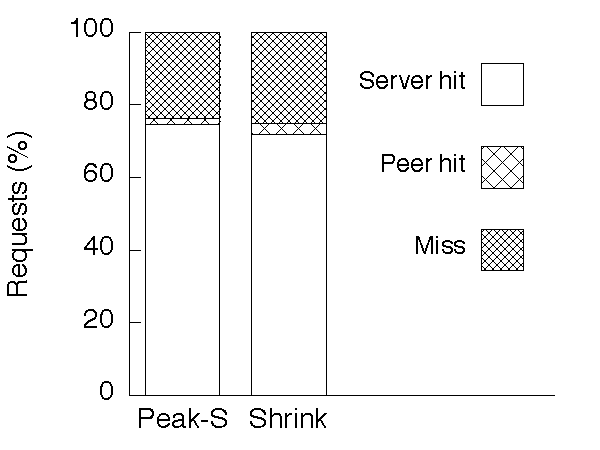
\includegraphics[scale=0.5]{graphs/final/sim-hitrate.pdf}
%\caption{[Simulator] \shrink\ increases miss rates by 1.5\% over \peakS\ over a one-week long trace showing that energy optimization in \cdc s hurts cache hit rates by a small margin. }
%\label{fig:sim-hitrate}
%\end{minipage}
%\hspace{0.5cm}
%\begin{minipage}{0.3\textwidth}
%\centering
%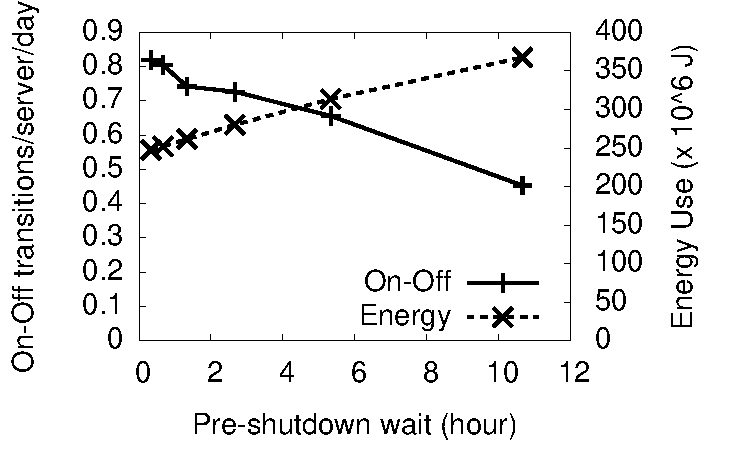
\includegraphics[scale=0.5]{graphs/final/onoff.pdf}
%\caption{[Simulator] Pre-shutdown wait interval ($W$) between 30 min \& 1 hour keeps on-off transition rate close to 1/server/day and with only a small increase in energy use over $W$ = 1 min.}
%\label{fig:sim-onoffrate}
%\end{minipage}
%\hspace{0.5cm}
%\begin{minipage}{0.3\textwidth}
%\centering
%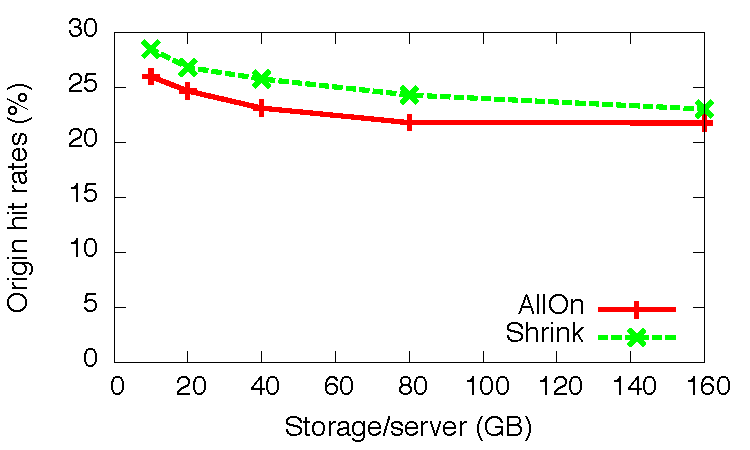
\includegraphics[scale=0.5]{graphs/final/storage.pdf}
%\caption{[Simulator] Difference between miss rates for both \shrink\ and \peakS\ is consistent despite variations in storage capacity.}
%\label{fig:sim-storage-vs-hitrate}
%\end{minipage}
%\end{figure*}

\subsubsection{Trace-based experiments}
\label{sec:simulation}
%The following are the goals of our trace-based experiments: (1) Quantify energy savings of server consolidation over the complete duration of the trace for a given server utilization limit expected to cause a small impact in response time.
%(2) Evaluate the potential benefit of cooperative caching among servers in a \cdc\ assuming that a cache-coordination protocol with a much smaller overhead can be developed in future. 
%(3) Quantify the tradeoff between energy savings and reliability by varying the pre-shutdown wait interval $W$.
%(4) Analyze the sensitivity of hit rates to a server's storage capacity.

\textbf{Methodology:} We conduct experiments for a \cdc\ with 16 servers for the week-long Akamai trace. The capacity of each server is defined in terms of network traffic it can support. The rate of network traffic generated by a request is a constant equal to the client bandwidth reported in the Akamai trace. To be able to fit the simulator process in the memory on our machine (32 GB), we filtered requests for one-eighth of the content from the trace. Accordingly, we scale down  the capacity of each server to be 150 Mbps, and the cache size per server to be 150 GB. Since trace-based experiments do not provide an accurate estimate of response times, we used a fixed server utilization limit $U$ = 0.65 for our experiments, which is expected to cause a small response time inflation (Figure \ref{fig:ec2-other} (right)). 
The cache hit rates of our simulator's LRU caching and Squid differ by less than 2\% for the same workload and cache size. 


\begin{figure}
\centering
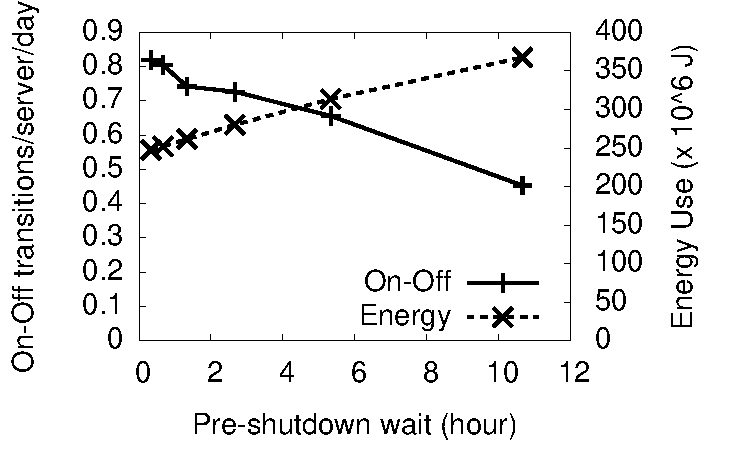
\includegraphics[scale=0.4]{graphs/final/onoff.pdf}
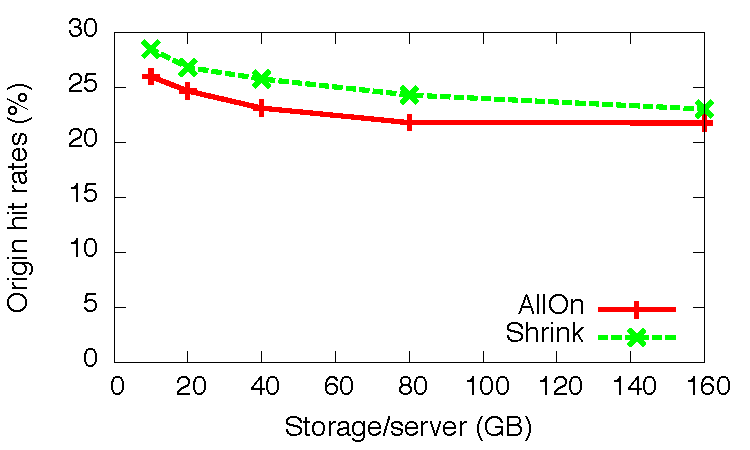
\includegraphics[scale=0.4]{graphs/final/storage.pdf}
\caption{[Simulator] [Left] Pre-shutdown wait interval between 30 min \& 1 hour keeps on-off transition rate close to 1/server/day. [Right] Comparison of miss rates for varying amounts of storage.}
\label{fig:sim-onoffrate}
\end{figure}
\textbf{Impact on hardware reliability:} Figure \ref{fig:sim-onoffrate} (left) shows the rate of on-off transitions per server and the corresponding energy savings is achievable. We find that a short pre-shutdown wait interval $W$ = 1 min hurts hardware reliability by increasing the rate of server transitions to more than 20/server/day. On the other hand, a  high $W$ = 4 hours reduces server transition rate to 0.81/server/day, but increases energy use by nearly 45\% over $W$ = 1 min.  The sweet spot for pre-shutdown wait interval is between 30 min to 1 hour, where increase in energy use over $W$ = 1 min is between 12\% and 15\%  but most of the reduction in on-off transition rates can still be achieved.

\textbf{Storage vs. cache miss rates:} To determine the sensitivity of miss rates to available storage, we evaluate \peakS\  and \shrink\ for varying amount of storage from 10 GB/server to 160 GB/server and present results in Figure \ref{fig:sim-onoffrate} (right). We remark that we have scaled down the CDN trace and hence the storage by a 8$\times$ factor, i.e., we would have provisioned 1.28 TB storage instead of 160 GB if we were to experiment with the full trace.  As storage reduces, the miss rates increase as expected. But, the relative difference between miss rates for both \shrink\ and \peakS\  remains nearly the same even on reducing the storage to 10 GB, e.g., \shrink's miss rates are 10.3\% higher than that of \peakS\  for 160 GB storage and are 9.6\% higher than that of \peakS\  for 10 GB storage. Thus, we conclude that server consolidation schemes are expected to increase datacenter miss rates by a small fraction within the range of storage typically available on server-class machines. 

\textbf{Cooperative caching benefit:} We evaluate the potential benefit of cooperative caching among servers in a \cdc\ assuming that a cache-coordination protocol with a much smaller overhead can be developed in future. The hit rates at cache peers  are 1.65\% for \peakS\  and 3.02\% for \shrink, which suggests that cooperative caching among datacenter servers, if implemented efficiently, could reduce the impact of energy optimization schemes by a small margin. 
%We present other results from trace-based experiments here. 
%(1) Over a one-week long trace. \shrink\ provides 37\% energy savings over \peakS. (2) 

%\textbf{Energy savings and cache hit rates:}
%We have compared the energy use of \shrink\ against other schemes over a one-week long trace. \shrink\ provides 37\% energy savings over \peakS\ in that experiment. We skip a detailed discussion of the results noting that energy use of other schemes are qualitatively similar to that observed in the experiment on EC2.
%
%Figure \ref{fig:sim-hitrate} compares the server hit rates, peer hit rates and miss rates. We make two key observations from this graph. First, there is less than 1.5\% difference in miss rates between \shrink\ and \peakS\  scheme, which supports our earlier observation in prototype-based experiments that \shrink's energy optimization does cause a significant increase in miss rates.  Second, we note that peer hit rates are 1.65\% for \peakS\  and 3.02\% for \shrink, which suggests that cooperative caching among datacenter servers could reduce the impact of energy optimization schemes by a small margin. Implementing a cooperative caching scheme with a low overhead is a topic of future work.




\eat{
%\begin{figure}
%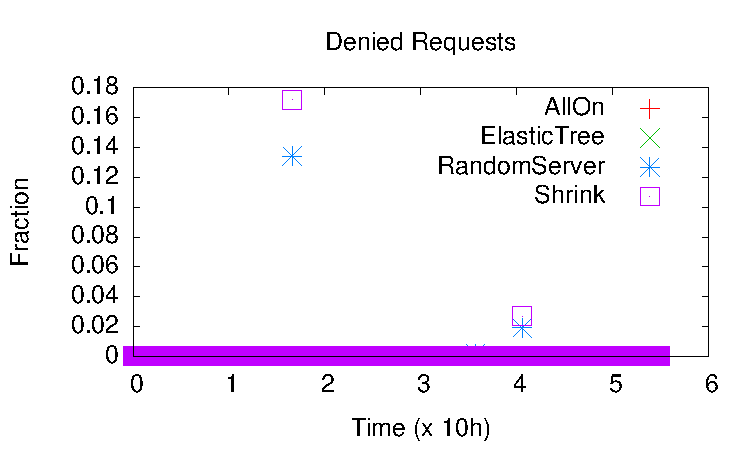
\includegraphics[scale=0.6]{graphs/server-logs/denied.pdf}
%\caption{Fraction of requests that are denied. \peakS\  scheme denies no requests throughout the experiment, whereas other schemes have a non-zero denied requests in a few time intervals. Both intervals  where requests are denied happened in cases of sudden spikes in load during night time.}
%\label{fig:sim-availability}
%\end{figure}

Figure \ref{fig:sim-availability} shows the fraction of requests that are denied due to server unavailability. Each data point represents denied requests in a 5-min interval. We find that the \peakS\  scheme has no denied requests throughout the experiment, i.e., it has 100\% availability. \shrink\ also has 100\% in all time intervals, except for two. Further analysis showed that both these intervals occured in late-night hours between 2 AM and 4 AM when there was unexpected spike in load that was 4 times the expected load in that interval. The active servers at that time did not sufficient enough resources to handle the request load. Thus, there was a brief period of unavailability until more servers could be turned on. That server unavailability is near-perfect an encouraging sign for deploying server consolidation, but also shows that energy-optimizing schemes make a \cdc\ less tolerant to highly unpredictable increase in load. A possible way to reduce the impact of such unavailability is to keep servers in a sleep state instead of completely turning them off so that they can be turned on quickly if necessary. 
}

%\begin{figure}
%\centering
%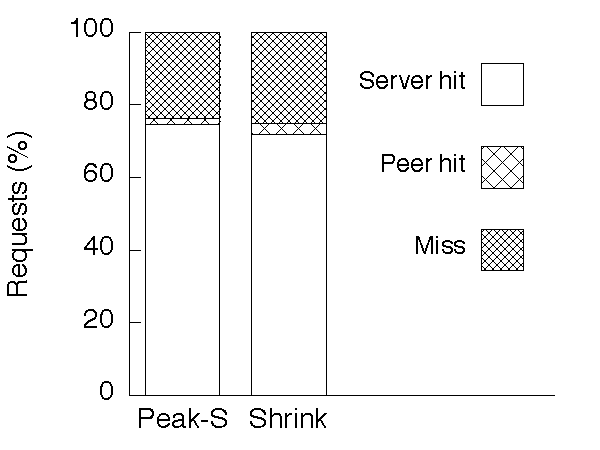
\includegraphics[scale=0.6]{graphs/final/sim-hitrate.pdf}
%\caption{[Simulator] \shrink\ increases miss rates by a small margin of 1.5\% over \peakS\ over a one-week long trace showing that energy optimization in \cdc s hurts cache performance by a small margin. }
%\label{fig:sim-hitrate}
%\end{figure}



%\begin{figure}
%\centering
%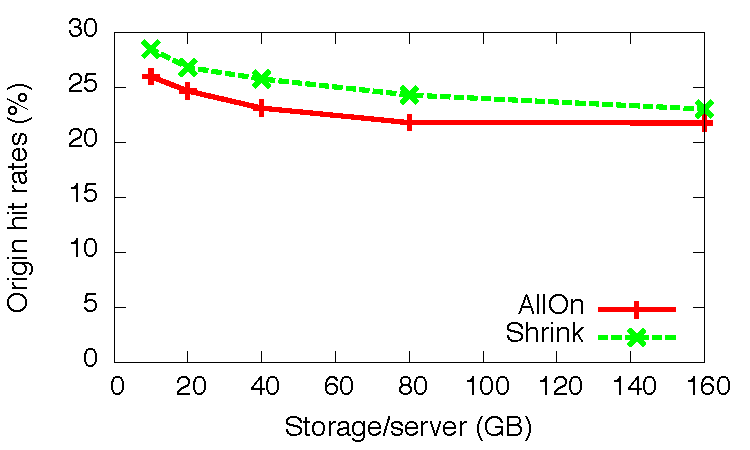
\includegraphics[scale=0.6]{graphs/final/storage.pdf}
%\caption{}
%\label{fig:sim-storage-vs-hitrate}
%\end{figure}




%!TEX root = shrink.tex

\section{Discussion}
\label{sec:discussion}

\textbf{Energy use vs. energy cost:} There are three types of \cdc s in terms of their energy cost to an operator. 

\emph{(1) Operator-owned facility:} If a \cdc\ operator owns the datacenter facility, it directly pays to the electricity companies based on its usage. In such datacenters, a reduction in energy use by \shrink\ is likely to bring a reduction in electricity costs as well.

\emph{(2) Co-location facility:} A \cdc\ at a co-location facility typically pays by the provisioned power and not the electricity used \cite{qureshi2009cutting}. Therefore, a reduction in energy use will not bring cost savings to \cdc\ operator with the existing pricing models. However, it is possible a \cdc\ operator may use the reduced energy as a leverage for negotiating a cheaper pricing. 

\emph{(3) Co-location inside ISP networks:} A \cdc\ at a co-location facility maintained by an ISP often has a symbiotic relation with the ISP, where the \cdc\ caches content to reduce the inter-domain traffic for the ISP while an ISP provides co-location free of charge \cite{google-caching}. In such \cdc s, energy savings do not translate to cost savings to the \cdc\ operator.  Although, energy savings do benefit the ISP, who eventually pays for the electricity.

The type of usage-based energy pricing also determines the cost savings for an operator. Specifically, we distinguish between flat rate pricing and time-of-use pricing \cite{pge-website}. With a flat rate pricing, a given percentage reduction in the energy use results in the same percentage reduction in the energy cost. With a time-of-use pricing, the percentage reduction in the energy use and the energy cost may not be the same. For example, if the peak load on a \cdc\ coincides with the peak hour of electricity prices, the percentage reduction in the energy cost would be lower than the percentage reduction in the energy use.

%\textbf{\shrink\ as a dynamic provisioning tool:} \shrink\ can be used as a dynamic provisioning tool by an operator that is running a content delivery site on infrastructure rented from a cloud-computing platform such as Amazon EC2. In such a setting, the operator may use \shrink\ to dynamically provision the number of active servers in accordance with incoming request load. In such a setting, the operator may not be able to perform network consolidation, but it can run the server energy optimization and load balancing sub-systems of \shrink\ and dynamically provision the number of active servers in accordance with incoming request load.  While functioning as a dynamic provisioning tool, \shrink\ can help reduce infrastructure costs for the operator.

\textbf{Impact on web-page load time:} Our prototype-based experiments evaluate the response time for individual HTTP requests, and hence do not capture a key metric that is more relevant from an end-user's perspective: web-page load time. However, we expect the inflation in web-page load time to be lower than the inflation in response times given that computation in web browsers constitutes up to 35\% of the critical path of a web-page load time \cite{wprof}.



\section{Related work}

Our effort distinguishes from prior work in quantifying the energy-response time tradeoff  in \cdc s, presenting the design and implementation of a system to leverage this tradeoff and proposing a network-aware server consolidation scheme to reduce network energy use.  Prior work on reducing energy of datacenters can be divided into three topics: (1) power-proportionality of servers and switches.  (2) server and network consolidation in a datacenter and (3) global load balancing across datacenters.

\textbf{Power-proportional servers and switches:}  Several efforts have focused on reducing energy use of a server's sub-systems such as CPU \cite{dvfs}, disk \cite{lu1999adaptive}, and memory \cite{fan2001memory}. Similarly, Nedevschi et al. \cite{Nedevschi08} study power management for switches that support sleep states or several power/performance states similar to CPUs. Nonetheless, today's servers and switches are far from power-proportional. Mahadevan et al. show that networking equipment consumes 62\%-91\% of their peak energy in idle state \cite{mahadevan2009power} and servers consume 32\% to 42\% of maximum power at a small utilization of 10\% \cite{spec}. Until the ideal of power-proportionality is achieved, consolidation remains a promising approach to save energy.

\textbf{Server consolidation:} Given the long line of work in server consolidation, our work does not focus on saving more energy than the existing consolidation schemes, but instead on accurately quantifying the impact on response times of a simple consolidation scheme.
%Both analytical and experimental studies of server consolidation have been previously explored. 

%A long line of work has studied consolidation techniques to reduce datacenter energy, including efforts that are analytical in nature as well as implementation-based efforts. 

The analytical work in this area shares similar goals as us.  Lin et al. \cite{lin12} propose an algorithm for optimizing a cost metric that incorporates energy costs, on-off switching costs and cost of degradation in performance. Mathew et al. \cite{mathew12} propose an algorithm that balances energy use, reliability and availability of servers, which they evaluate based on load traces from Akamai datacenters. In comparison, our implementation-based approach enables us to accurately model the relation between server utilization and response time, impact of server consolidation on cache hit rates, and non-ideal load balancing, to accurately quantify the impact of consolidation on response time for \cdc s.

Several efforts have conducted an implementation-based evaluation of server consolidation for stateless systems. Chase et al. \cite{chase2001managing} allocate resources among multiple co-hosted services in a cluster while reducing energy via consolidation. Pinheiro's \cite{pinheiro2001load} system proposes consolidation and load balancing algorithms given a bound on the performance degradation that is acceptable.  Rajamani et al. \cite{rajamani2003evaluating} evaluate consolidation schemes for a modified TPC-W workload. In comparison, our effort focuses on \cdc s that maintain a large amount of state in the form of cached content. In \cdc s, the effect of consolidation on response times cannot be evaluated accurately without accounting for the effect of consolidation on the availability of cached content and the resulting cache hit rates.
%One of our key findings is that consolidation results in a small impact on cache hit rates, which helps \shrink\ achieve a good energy-response time tradeoff.

Trushkowsky et al. \cite{Trushkowsky:2011}  dynamically allocate servers and reconfigure the data stored on the servers to meet service-level objectives such as 99-th percentile request latency.  However, there are two key differences between their work and ours. First, they focus  on a workload exclusively of small (256B) objects stored in-memory, whereas  \cdc s need to deal with orders of magnitude of heterogeneity in object sizes and extensively use a disk cache to improve hit rates.  Second, their system appears to be a backend data store, which always has content available within the datacenter. In comparison, \cdc s have a significant fraction of traffic to remote datacenters due to cache misses, and the impact of consolidation on response time in \cdc s depends on the increase in traffic to remote datacenters that consolidation causes. For these reasons, it is not clear if their findings on the impact of dynamic server allocation on request latency would be applicable for \cdc s.
%One of our key findings is that consolidation results in a small increase in cache miss rates, which helps \shrink\ achieve a good energy-response time tradeoff. 

%\TBD{we optimize network energy use also}

\textbf{Network consolidation:} Network  consolidation has been studied for both wide-area and data center networks \cite{response, elasticTree, greenTE, Chiaraviglio, Andrews}. Network consolidation concentrates traffic, represented in the form of a traffic matrix, on a subset of links and switches, and turns off remaining switches and links to save energy. Our work differentiates from prior work in two ways. First, prior work evaluates schemes mostly using traffic engineering metrics such as link utilization, while we evaluate actual end user response time for a real application and show that network consolidation can be performed with a small performance impact in \cdc s. Second, we show network consolidation is closely related to server consolidation. Our network-aware server consolidation saves up to 45\% more network energy over a network-unaware server consolidation scheme.
%network-aware server consolidation increase the potential savings that a network consolidation scheme can achieve. 
%
%
%
%
%
%
% with little effort on measuring response times for real applications
%
%While previous work has studied server and network consolidation as independent problems, we show that these problems are closely related. For the same number of servers, which set of servers is chosen affects potential energy savings that a network consolidation scheme can achieve. Further, we propose a simple network-aware server consolidation scheme saves up to 45\% more network energy over a network-unaware server consolidation scheme.

\textbf{Global load balancing:} Many papers \cite{Liu11,qureshi2009cutting,Gao12,Rao10}  have shown that geographical load-balancing across data centers can exploit the differences in electricity prices and in renewable energy availability at various locations to reduce energy costs, energy use, or non-renewable energy use.  In comparison, our work focus on improving energy-efficiency of a single \cdc\ by the use of consolidation. We believe that global load balancing can complement \shrink\ in reducing energy use and its cost across datacenters.

%!TEX root = shrink.tex
\section{Conclusions}
Content datacenters used for storing and serving content to end-users are common today. A major barrier to  widespread adoption of server and network consolidation is \cdc\ operators' concern on the impact on SLAs or user-perceived latencies. Our work takes a step towards addressing this concern by presenting a model to quantify the energy savings vs. latency inflation trade-off in \cdc s.  A key insight, supported via experiments, is that despite server consolidation, cache hit rates remain close to an unconsolidated datacenter,  which helps mitigate the impact of consolidation on user-perceived latencies. We have designed and implemented \shrink, a system that leverages this tradeoff to yield significant energy savings while affecting user-perceived latencies in a controlled manner. \shrink's novel network-aware server consolidation algorithm reduces network energy use by up to 42\% compared to network-unaware server consolidation schemes. \shrink, in experiments based on content access traces from an Akamai datacenter, reduced energy use by 35\% compared to a baseline scheme that keeps entire datacenter always on while increasing mean latency by 8\% over it. Overall, our findings encourage deployment of consolidation techniques to reduce \cdc\ energy use.




\chapter{Network energy lower bound}
\label{sec:netlb}
We derive lower bounds on the network energy use for FatTree \cite{fattree} and VL2 \cite{vl2} under the constraint that $n$  servers that are active must be able to simultaneously send traffic to clients equal to the external bandwidth $E$ via the set of active switches only.

\textbf{VL2:} Let the energy use of each core, aggregation and ToR switch be $PC$, $PA$ and $PT$ respectively.
Let $L$ be the capacity of links between each pair of core and aggregation switches. 
If  $c$ core switches and $a$ aggregation switches be active, then
the maximum number of servers that can be supported is $ \textit{nmax} = (a\times c\times L/E)$ and the total energy use of core and aggregation switches is $\textit{etotal} = (c \times PC + a \times PA)$. 
We select the optimal values of $\textit{a\_opt}$ and $\textit{c\_opt}$ (by enumerating all values) such that \textit{etotal} is minimized under the constraint that $\textit{nmax} > n$. 
Assuming each ToR switch connects to $k$ servers,  the minimum number of ToR switches needed is $\lceil n/k \rceil$. 
Thus, a lower bound on the total network energy use is $(\lceil n/k \rceil PT) + (\textit{c\_opt} \times PC + \textit{a\_opt} \times PA)$.


\textbf{FatTree:} Switches are identical in a FatTree. So, a lower bound the number of active switches gives a lower bound on network energy use also.




Let $m_1, \cdots m_k$ be the active servers in the $k$ pods so that $m_1 + \cdots + m_k = n$.  In a pod with $m$ active servers, at least $2 \sqrt{m}$ switches must be active. Thus, a total of $(2 (\sqrt{m_1} + \cdots + \sqrt{m_k} ))$ pod switches must be active. 

Let $c$ be the number of active core switches. We claim that the number of active servers in any pod can at most be $c$. The reason is that a core switch has only one link to switches in each pod, and hence can receive traffic from only one server sending traffic at its outgoing link capacity to external clients. The values of $m_1, \cdots m_k$ that minimizes the number of active pod switches is given by $m_1 = m_2 = \cdots = m_l = c$,  $m_{l+1} = (n \bmod c)$, and $m_{l+2} = m_{l+3} = \cdots  m_{k} = 0$, where $l = \lfloor n/c \rfloor$.  Let $p$ be minimum number of active pod switches thus computed. Then, the minimum number of total active switches active is given by $(p+c)$.



% If $m_1, \cdots m_k$ are the active servers in the $k$ pods, then a total of $(2 (\sqrt{m_1} + \cdots + \sqrt{m_k} ))$ pod switches must be active.


%If $c$ core switches are active, the values of $m_1, \cdots m_k$ where $m_1 + \cdots + m_k = n$ that minimizes the number of active pod switches is given by $m_1 = m_2 = \cdots = m_l = c$,  $m_{l+1} = (n \bmod c)$, and $m_{l+2} = m_{l+3} = \cdots  m_{k} = 0$, where $l = \lfloor n/c \rfloor$.  Let $p$ be minimum number of active pod switches thus computed. Then, the minimum number of total active switches active is given by $(p+c)$.

Computing the minimum number of switches for all possible values of $c\ (c \leq n, c \leq k^2/4)$ and taking their minimum gives a lower bound on the number of active switches for this topology.

%taking the least possible value of $c$ for which 



%\textbf{FatTree:} A $k$-FatTree is built using identical switches with $k$ ports of equal capacity. We compute the least number of core, upper-level pod and lower-level pod switches that are active. Each lower-level pod switch is connected to $k/2$ servers. Therefore, at least $\lceil n/(k/2) \rceil$ lower-level pod switches are active. Each upper-level pod switch has $k/2$ ports to lower-level pod switches and hence it can receive traffic from at most $k/2$ servers sending traffic at their outgoing link capacity to external clients. Thus, $\lceil n/(k/2) \rceil$ upper-level pod switches are active. Each core switch has only one link to switch in each pod, and hence can receive traffic from only one server sending traffic at its outgoing link capacity to external clients. Thus, the minimum number of core switches is equal to the maximum number of servers that are active in any pod. There at least one out of $k$ pods has at least $\lceil n/k \rceil$ active servers. In total, $(\lceil n/k \rceil + 2 \lceil n/(k/2) \rceil)$ switches must be active.

%Since each  lower-level pod switch and upper-level pod switch supports at most $k/2$ active servers, at least $\lceil n/(k/2) \rceil $ lower-level pod switches and upper-level pod switches must be active.



\eat{
\section{Characteristic time approx.}
\label{sec:approximation}
The characteristic-time approximation computes the hit rates of each content served by an LRU cache \cite{che2002hierarchical}. This approximation has proved accurate for workloads with a Zipf content popularity distribution.  Let $O$ be the set of unit-sized content served by a cache of size $S$ units and $l_j$ denote the request rate for content $j \in O$. Solving the equations below using fixed-point approximation yields the hit rates, $h_j$, for content $j \in O$ and, $T$, the characteristic time of the cache. The cache hit rate across all content is $\frac{\sum_{j\in O}h_j l_j}{\sum_{j\in O} l_j}$. 
\[h_i = 1 - e^{l_j T}\quad \forall j \in O\]
\[\sum_{j \in O} h_j = S \]
}

\eat{
\section{MIP for energy optimal node selection}
\label{sec:optimal}

We describe the optimal strategy for selecting servers and switches that minimize network energy use given the number of active servers in a datacenter and the traffic flow from each active server to the client node. Let $N$ be the set of all nodes in a 3-level datacenter topology, with servers $S$ as leaves  and switches $R$, and a virtual client node $c$. We assume a tree-like datacenter topology in which all links are between nodes with a difference of one in their heights. The virtual client node is the root node in the topology is connected via infinite capacity links to all core-switches. Let $E$ be the set of unidirectional edges in the datacenter in the direction from leaves to root, such that $e_{ij}$ is the link from node $i\in N$ to node $j \in N$ with link capacity $C_{ij}$. Let $O(j)$ and $I(j)$ are incoming and outgoing links at switch $j$. 
 Let $f$ be the traffic flow from each active server to the client node. Further, the number of servers to be kept active is $A$. Switch $i \in R$ consumes power $P_i$ and the power use of ports at the two ends of link $e_{ij}$ $Q_{ij}$  and $Q_{ji}$.  Let $s_i$ denote a binary variable indicating whether server $i \in S$ is turned on. Let $r_i$ denote a binary variable indicating whether switch $i \in R$ is turned on. Let, $t_{ij}$ denote a  binary variable indicating whether link $e_{ij} \in E$ is active.


\[\textit{Minimize:}\quad\sum_{i \in R} r_i P_i+\sum_{e_{ij} \in E} t_{ij} (Q_{ij} + Q_{ji})\]

\emph{Constraints:}

\[\sum_{i \in R} s_i = A \quad\textit{\small{\# Number of active servers is A}}\]
\[f_{ij} = s_i f\ \ \forall i \in S, j \in \textit{O(i)}\ \  \textit{\small{\# Active server sends f traffic units}}\]
\[\sum_{e_{ij} \in O(j)}f_{ij}=\sum_{e_{jk} \in I(j)} f_{jk}\ \forall j \in R \ \textit{\small{\# Flow conservation at switch}}\]
\[f_{ij} \leq C_{ij} t_{ij} \ \forall e_{ij} \in E\ \textit{\small{\# Link, if on, carries traffic up to capacity}}\]
\[t_{ij} \leq r_j \  \forall j \in R, e_{ij} \in I(j)\ \textit{\small{\# Incoming links off, if switch is off}}\]
\[t_{jk} \leq r_j \  \forall j \in R, e_{jk} \in O(j)\ \textit{\small{\# Outgoing links off, if switch is off}}\]
\[r_j \leq \sum_{e_{ij} \in I(j) } t_{ij} \ \textit{\small{\# If all incoming links are active, switch is off}}\]
%\[r_j \leq \sum_{e_{jk} \in  O(j) } t_{jk}\ \textit{\# } \]
%\[s_i, r_k,  = \{0,1\} \forall i \in S, r_i = \{0,1\} \forall i \in R, t_{ij} = \{0,1\} \forall e_{ij} \in E\]

}


\vfill\eject
\bibliographystyle{abbrv}
\bibliography{shrink} 

\end{document}

%%!TEX root = Main.tex
\vsp
\section{Introduction}
\label{sec:intro}
``Mobile'' has long arrived, but the Internet remains unmoved. Today, there is roughly one cellphone per human; the number of smartphones sold last year alone roughly equals the number of wired hosts on the Internet \cite{gartner}; and the total traffic originated by mobiles is poised to approach that by wired devices \cite{cisco-vni}. However, the current Internet continues to operate as it did when dominated by tethered hosts, simply ignoring frequent endpoint mobility.

Today, an application developer can not easily initiate communication with a smartphone even when it has a public IP address as there is no global infrastructure support for locating it. Applications like smartphone notification systems, playback video, or cloud storage have to develop application-level support to enable a seamless experience for their users even as they change addresses several times a day, or let connections break (as popular VoIP apps do today).   The lack of intrinsic support for mobility means that developers are forced to redundantly develop and maintain common-case functionality. Furthermore, we are paying an unknowable price in terms of long-term growth and innovation by straitjacketing communication initiation to be unidirectional.

%The lack of intrinsic support for mobility means that we are paying an unknowable price in terms of stymied application innovation and growth by forcing developers to redundantly develop common-case functionality, and forcing communication initiation to be mostly unidirectional.

%A mobile user might reasonably expect that a voice-over-IP call she initiated through one WiFi network would continue uninterrupted if she switched to a different WiFi or  cellular network; or expect a file transfer she initiated at home on her laptop to resume when she opens it at work in a disruption-tolerant manner. Today, one can not easily initiate communication with a smartphone (even when it has a publicly visible IP address) because there is no global infrastructure support for locating it. Of course, application developers can design around these limitations, as do applications like Skype\tbd{I don't think Skype actually supports this today. Netflix maybe a better example.}, Dropbox, and smartphone notification systems respectively for the above scenarios. However, the lack of intrinsic support for mobility means that we are paying an unknowable price in terms of stymied application innovation and growth by forcing developers to redundantly develop common-case functionality, and forcing communication initiation to be mostly unidirectional.

%Many before us have criticized the Internet architecture's poor support not only for mobility but also for multihoming \cite{HIP,LISP,HAIR}, content retrieval \cite{DONA,LNA,CCN}, and security \cite{AIP,XIA,MobilityFirst-UMASS}. A common criticism is the Internet's so-called conflation of identity and location. The Internet uses an IP address both to represent the identity of an interface as well as its network location, which is problematic for mobility (same identity, changing locations) and multihoming (single identity, multiple locations) of devices, services, or content. Applications today are forced to know and care about changing IP addresses as the transport and network layers only provide a primitive to establish  connections between IP addresses, not application-friendly names. It is commonly accepted wisdom that a cleaner separation of identity and location is instrumental to fixing these problems.

%Many before us have criticized the Internet architecture's poor support not only for mobility but also for multihoming \cite{HIP,LISP,HAIR}, content retrieval \cite{DONA,LNA,CCN}, and security \cite{AIP,XIA,MobilityFirst}. A common criticism is the Internet's so-called conflation of identity and location. The Internet uses an IP address both to represent the identity of an interface as well as its network location, which is problematic for mobility (same identity, changing locations) and multihoming (single identity, multiple locations) of devices, services, or content. Applications today are forced to know and care about changing IP addresses as the transport and network layers only provide a primitive to establish  connections between IP addresses, not application-friendly names. It is commonly accepted wisdom that a cleaner separation of identity and location is instrumental to fixing these problems.

Many before us have criticized the Internet architecture's poor support for mobility as well as multihoming \cite{HIP,LISP,HAIR,MobilityFirst}. A common criticism is the Internet's so-called conflation of identity and location, i.e., the use of an IP address both to represent the identity of an interface as well as its network location, which is problematic for mobility (same identity, changing locations) and multihoming (single identity, multiple locations). It is commonly accepted wisdom that a cleaner separation of identity and location is instrumental to fixing these problems. However, the Internet does separate identities (domain-names) from network locations (IP addresses) through DNS. Most high-level programming languages also provide syntactic sugar to \verb+connect+ to names remaining oblivious to IP addresses; and %name owners can and do employ managed DNS services or CDNs to return the best-positioned network location corresponding to multi-homed names. 
techniques from a long line of work on connection migration could be employed to seamlessly handle mid-connection mobility.

But a key missing element from this package today is a distributed name resolution infrastructure that can scale to orders of magnitude higher update rates than envisioned when DNS was created. To appreciate the envisioned scale, consider tens of billions of mobile identifiers changing network addresses at least tens of times per day. DNS's heavy reliance on TTL-based caching, a key strength recognized by its creators, researchers, and operators alike, poses a significant handicap by increasing update propagation delays, load on name servers, and overall client-perceived latency. It is not uncommon for DNS update propagation to take a day or more, resulting in long  outage times when online services have to be moved unexpectedly, prompting cries for help on operator forums \cite{serverfault,dns-long-update}. A less widely noted limitation of DNS is its reliance on hierarchical names for scaling via federation and its single root of trust, which constrains mobile applications from selecting arbitrary application-specific names (as elaborated in $\S$\ref{sec:whyNotDNS} and $\S$\ref{sec:design_overview}).

 %   Mobile has arrived, but the Internet is still static.

%    Reason 1: identity-location conflation. A number of solutions proposed to address this.

%    Reason 2: identity-location conflation would not be that problematic with an efficient resolution infrastructure. The Internet does separate human-readable ``names" from ``locations" or IP addresses through DNS. However, the design of the DNS resolution infrastructure implicitly assumes rare mobility. Indeed, Mockapetris and Dunlap allude to this by justifying the design decision of departing from the Xerox PARC Grapevine system... quote here.


Our position is that seamless support for mobility requires a logically centralized global name service that rapidly translates identities to locations irrespective of how exactly identities and locations are individually represented. Our primary contribution is the design, implementation, and evaluation of \auspice, a distributed system that helps address this challenge. Compared to today's ICANN/DNS-based approach, our approach cleanly separates name resolution from adjudication and certification issues ($\S$\ref{sec:design_overview}). \auspice\ is also deployable as a managed DNS provider in today's Internet; compared to them, a key strength of \auspice\ is a {\em demand-aware} replica placement engine that significantly reduces the {\em time-to-connect} to mobile destinations in a cost-effective manner. Under light load, \auspice's demand-aware replica placement aggressively uses available resources to massively replicate name records, while under heavy load, it carefully controls the number and choice of replica locations based on the read-write patterns and pockets of high demand for each name.

%low lookup latency, low update cost, and high availability.  \auspice\ achieves low-latency by inferring pockets of high demand for a name so as to create replicas of  for that name close to them. \auspice\ achieves low latency,  low update cost,  and high availability using a placement optimization algorithm that (1) controls the number of replicas based on the observed read and write rates, and (2) determines where to place replicas based both on the inferred pockets of demand and the aggregate load at node locations near those pockets. 



We have implemented a prototype of \auspice\ as a geo-distributed key-value store to serve as a flexible name resolution service for the current Internet as well as several ``future'' Internet or endpoint architectures such as MobilityFirst\cite{MobilityFirst}, HIP\cite{HIP}, or XIA\cite{XIA}. We have extensively evaluated \auspice\  using a combination of Planetlab, emulation clusters, and Amazon EC2.  Our contributions are as follows.
\begin{enumerate}
\item A case for a global name service as an indispensable part of any Internetwork design with intrinsic support for high mobility ($\S$\ref{sec:case}).
\vsp
\item \auspice, a scalable, geo-distributed, federated global name service that significantly reduces the time-to-connect under any given resource constraints despite high mobility and arbitrary endpoint identifiers ($\S$\ref{sec:design},$\S$\ref{sec:eval}). 
\figvsp
\item A proof-of-concept demonstration of intrinsic support for---{\em(i)} all four types of endpoint mobility; {\em(ii)} novel context-aware delivery primitives that generalize name- or address-based communication---over the current Internet as well as MobilityFirst \cite{MobilityFirst} ($\S$\ref{sec:e2e}). 
\vsp
\item Comparison against several best-of-breed managed DNS services showing that \auspice's  demand-aware approach significantly lowers time-to-connect and/or update cost even for today's (hardly mobile) domain names ($\S$\ref{sec:managed}).
\vsp
\end{enumerate}
\vsp

To provide a historical perspective, until the early 80s, the Internet relied on a system called \verb+HOSTS.TXT+ for name resolution, which was simply a centrally maintained text file distributed to all hosts. The current Internet's distributed DNS  arose in response to the rapidly increasing file size and distribution costs. Mockapetris and Dunlap \cite{DNS} point to TTL-based caching to reduce load and response times as a key strength, noting that ``{\em{the XEROX system {\em [Grapevine \cite{grapevine}]} was then ... the most sophisticated name service in existence, but it was not clear that its heavy use of replication, light use of caching ... were appropriate}}''. We have since come a full circle, turning to  active replication ($\S$\ref{sec:whyNotDNS}) in \auspice\ in order to address the challenges of mobility, a concern that wasn't particularly pressing  in the 80s. Compared to classical systems like Grapevine or ClearingHouse, \auspice\ enables support for automated {\em demand-aware} replica placement for {\em arbitrary names} (using several modern design elements such as consensus, the key-value abstraction, self-certifying names, consistent hashing, etc).  \auspice, through its support for context-aware delivery, is also a step towards addressing some of the challenges to which Lampson alludes on representing ``descriptive names" \cite{Lampson}.


\eat{
\emph{Low update cost:} \auspice\ reduces updates costs by nearly an order of magnitude over a replicate-everywhere strategy in a live deployment and yet achieves nearly identical lookup latencies.
\item
\emph{Load balance:} Over a wide range of loads, \auspice's achieves 2X - 4.5X lower lookup latencies over a random replication scheme, and  5.4X - 11.2X lower latency than a DHT-based replication scheme. Due to its lower update costs, \auspice\ can sustain 18$\times$ higher loads than a replicate everywhere strategy.
}

%\begin{itemize}
%\item
%Locality-aware placement helps \auspice\ achieve 5$\times$ lower median lookup latency than a DHT-based replication scheme. 
%\vspace{-0.1in}
%\item
%\auspice\ reduces updates costs by nearly an order of magnitude over a replicate-everywhere strategy in a live deployment and yet achieves nearly identical query latencies.\vspace{-0.1in}
%\item
%\auspice's load-aware design achieves 1.2$\times$-3.3$\times$ lower lookup latencies than a locality-unaware scheme over a wide range of load scenarios.\vspace{-0.1in}
%\item
%\auspice\ achieves  DNS lookup latencies comparable to a leading managed DNS provider today even with only one third the number of name resolvers.
%\end{itemize}

%\begin{enumerate}
%\item  \auspice's locality-aware and load-aware replication achieves  5$\times$ lower latency than Codons, a proposed DHT-based replication alternative to DNS.
%\item \auspice\ reduces update costs
%\end{enumerate}
\eat {

The Internet's tremendous success and our maturing realization of its shortcomings have attracted significant research attention towards a clean-slate redesign of the Internet's architecture (e.g., NSF FIND \cite{FIND}, GENI\cite{GENI}, FIA\cite{FIA}). A number of the shortcomings of the current Internet can be traced back to issues related to {\em naming}, a central component of any distributed system design. In the current Internet, network entities are identified using IP addresses and the Domain Name System (DNS) resolves human-readable end-host names to IP addresses. Although this design has proven to be surprisingly malleable, it suffers from two sets of fundamental problems, both of which are  exacerbated by the the exponential growth of mobile devices and applications today.


The first results from the conflation of identity and location within an IP address, a design decision roundly criticized by many \cite{ROFL,Saltzer:1993:NBN:RFC1498,HIP,FARA,LNAI}. Using an IP address to identify a network interface as well as the network location of that interface complicates {\em mobility}---when the location changes but not the identity---and {\em multihoming}---when a single identity simultaneously resides at multiple locations---e.g., being simultaneously connected to a cellular and WiFi access network. With roughly 5 billion mobile devices worldwide today \cite{gartner}  (over a billion of which are IP-capable) compared to barely a billion tethered hosts \cite{CIA}, mobility and multihoming are the norm, not an exception. Conflating identity and location also poses a serious but  less widely acknowledged security challenge, namely, verifying that an interface indeed has the identity it claims. Unlike human-readable names that are bound to public keys by trusted certification authorities in order to enable application-level authentication today, IP addresses are harder to certify, especially when they change many times a day. As a result, we largely make do today with application-level security over a network that can be easily rendered unavailable by spoofing or hijacking of IP addresses.



The second results from the architecture of DNS, a critical part of the Internet's core infrastructure. The design of DNS in the Internet's early days implicitly assumed tethered hosts or infrequently changing addresses to be the common case, an assumption evident in its heavy reliance on caching and timeout-based invalidations for scalability. An inevitable consequence of this design is that unanticipated updates to DNS resource records are slow; more than 40\% domain names have a TTL of a day or more \cite{codons}. Even for slow-changing records, DNS lookup times constitute a significant fraction of user-perceived response times, e.g., over 30\% of web objects incur a DNS lookup latency of over a second \cite{Jung,Huitema}. Deploying more passive local name sever caches can reduce lookup latencies, but this benefit comes at the cost of further increasing update propagation delays or update load in the system. These and other problems with DNS such as poor load balance and responsiveness to changing demand patterns, vulnerability to denial-of-service attacks, etc. have been well documented by researchers \cite{Pappas,codons,Brownlee,dnssec}.

Our primary contribution is the design and implementation of a global name service that addresses the above problems. This global name service is a central component of MobilityFirst, a clean-slate future Internet architecture that is primarily motivated by the dual concerns of {\em mobility} and {\em security}.
%two concerns that are remarkable both for their absence in the design philosophy underlying the current Internet \cite{Clark88} as well as their immense importance today. 
MobilityFirst cleanly separates identity and location using a {\em globally unique identifier} (GUID) that, unlike an IP address, is by design devoid of location or any other structured information. Information about a GUID's location or {\em network address} (NA) is maintained by the resolution service. Both GUID and NA are {\em self-certifying}, i.e., they are one-way hashes of public keys, allowing any network entity to authenticate an entity claiming to possess a GUID or NA. Thus, the structureless nature of these identifiers enhances mobility as well as security. Section \ref{sec:MF} describes how the name service helps efficiently support a number of other functions such as multihoming, incoming traffic engineering, content retrieval, network mobility, multicast, etc.

%Key feature: low response times while respecting capacity constraints and consistency requirements. TBD.

A critical distributed systems challenge in realizing a global name service that supports mobility at scale  is the design and implementation of the infrastructure that quickly resolves identifiers to network addresses. To appreciate the scale, consider 10 billion identifiers (for mobile devices, services, content identifiers, or entire networks such as vehicular networks) moving across a 100 network addresses per day, i.e., a load of a million/sec for updates alone. Furthermore, the name service should process lookup queries quickly, requiring queries to be directed to a nearby replica that holds a consistent replica of the corresponding resource records. Finally, the service should balance the aggregate load across all names across the geographically distributed locations of the global name service. 

Our proposed solution to achieving all of the goals above---low latency, low update cost, and load balance---is a placement engine \auspice, that {\underline{\bf au}}tomates {\underline{\bf s}}ervice {\underline{\bf p}}lacement {\underline{\bf i}}n {\underline{\bf e}}lastic {\underline{\bf c}}louds. The \auspice\ engine is flexible in that it enables automated placement for cloud-hosted services that are more general (and in widespread use today) than name resolvers in a future Internet architecture. To ensure low response times, \auspice\ dynamically spawns or migrates service replicas close to pockets of high demand. To ensure low update cost and load balance under capacity constraints, \auspice\ controls the number and placement of service replicas using heuristic algorithms that are uncoordinated across services or a global optimization algorithm coordinated across all services by the hosting service provider.

We comprehensively evaluate \auspice\ using an implemented prototype on Planetlab and Amazon EC2. Also design custom simulator. Validate simulator. Case studies and results preview. TBD.

\paragraph{Roadmap} The rest of this paper is organized as follows. Section \ref{sec:MF} presents the naming subsystem in the MobilityFirst Internet architecture. Section \ref{sec:auspice} presents the design goals and architecture of an automated service replica placement system, \auspice, for geo-distributed cloud-hosted services and the instantiation of a global name service using it. Section \ref{sec:eval} describes the datasets used and the experimental evaluation of \auspice. Section \ref{sec:related} describes related work and Section \ref{sec:concl} concludes.

}


% application-centric comparison
\chapter{Traffic Engineering: An Application-Centric Comparison}
\label{ch:beyondmlu}

\section{Introduction}

\subsection{Shortcomings of link utilization metrics}

\subsection{Challenges in evaluating TE schemes}

\subsection{Results from an application-centric evaluation}

\subsection{Chapter organization}

Traditionally, traffic engineering (TE) has been studied as an optimization problem that takes as input a traffic matrix (TM) and seeks to compute routes so as to minimize a network cost function. The cost function is intended to capture the severity of congestion hotpsots based on link utilization levels. For example, the most widely used cost function, MLU, is simply the utilization of the most utilized link in the network \cite{COPE,TEXCP,MultiTM,Cohen}; others  sum over all links a convex function of their utilization  (so as to penalize highly utilized links more)  \cite{fortz2000internet,fortz2002traffic}. There are two implicit assumptions underlying this line of work. First, maintaining low link utilization improves user-perceived application performance under typical load conditions. Second, maintaining low link utilization increases the effective capacity of the network by enabling it to accommodate unexpected surges in the traffic demand.

Our work questions both of the above assumptions. The distinguishing aspect of our work is an application-centric approach to the problem: instead of posing TE as as optimization problem seeking to minimize link utilization, we focus on application performance metrics such as TCP throughput for elastic  traffic and quality-of-service metrics (e.g., MOS score for VoIP quality \cite{MOS-formula}) for inelastic traffic. Accordingly, our evaluation methodology is empirical: instead of relying on mathematical simulations based on linear programming or heuristic techniques for NP-complete problems, our experiments carefully and at scale simulate end-to-end application behavior so as to compare TE schemes with respect to their impact on application performance. 

Our application-centric and empirical approach reveals rather unexpected results. Our first finding is that metrics based on link utilization alone, and in particular MLU, are a poor proxy for application performance. For example, a TE scheme may incur twice the MLU of another TE scheme and yet achieve as good or better application performance. The key reason for this mismatch is that application performance is largely determined by end-to-end loss rate and delay, but link utilization does not capture them accurately. At typical Internet loads, and in fact until the utilization starts approaching the capacity, link loss rates remain negligibly small. This observation has also been confirmed by explicit measurements on Internet backbones \cite{ExpRouterBuffer}, and is consistent with studies on ISP backbones showing that over 90\% of all packet loss is caused by interdomain routing fluctuations as opposed to high utilization \cite{SprintStudy} and 90\% of TCP flows experience no packet loss \cite{SprintBackbone}. Furthermore, end-to-end Internet path delays are known to be largely determined by propagation delays as opposed to queueing delays \cite{SprintBackbone,SingleHopDelay}. 

As a result, we find that all state-of-the-art TE schemes achieve nearly identical application performance at typical Internet load levels. In fact, even static shortest-path routing with link weights inversely proportional to the capacity (\invcap) (i.e., no engineering at all) achieves the same application performance as optimal TE. Ironically, TE schemes that engineer for unexpected traffic spikes (e.g., COPE \cite{COPE}) consistently hurt TCP throughput despite achieving near-optimal MLU.

More surprisingly, we find that application adaptation to location diversity,  i.e., the ability to download content from multiple potential locations, blurs differences even in the achieved capacities of different TE schemes enabling all of them to be near-optimal. With location diversity, we find that the inverse of the MLU is no longer a meaningful metric of capacity. Instead, we formalize a new metric of the capacity achieved by a TE scheme called the {\em surge protection factor} (SPF) that captures the factor of increase in demand that can be sustained while accounting for location diversity. TE schemes calculate routing based on a measured traffic matrix to achieve a desired network cost, but application adaptation to location diversity changes the traffic matrix itself in response to a change in routing resulting a different network cost than expected. As a result, the optimal TE scheme with perfect knowledge of traffic matrix and sub-optimal TE schemes like OSPF weight-tuning \cite{fortz2000internet} end-up achieving the same SPF. Even the static routing scheme, \invcap, achieves an SPF at most 30\% worse than optimal TE.


The rest of the chapter is as follows. Section \ref{sec:locdiv-background} explains how location diversity changes the TE problem. Section \ref{sec:exp_setup} presents our simulation setup. Section \ref{sec:app_performance} compares the application performance of TE schemes and Section \ref{sec:capacity} compares their achieved capacity under location diversity. 


\section{Engineering traffic with location diversity}
\label{sec:locdiv-background}

This section introduces location diversity and proposes a new metric to quantify the capacity achieved by traffic engineering schemes with location diversity.


\subsection{Location diversity: Prevalence}

Location diversity, or the ability to download content from multiple potential locations, is widespread in the Internet today. Major commercial CDNs, e.g., Akamai \cite{Akamai}, Level-3 \cite{Level-3}, EdgeCast \cite{edgecast} etc., commonly replicate content at hundreds of locations and redirect users to the best server based on proximity or dynamic monitoring of server and network congestion \cite{akamai-detour}. Popular P2P applications such as BitTorrent \cite{bittorrentprotocol}, PPLive \cite{PPLive} download content simultaneously from many peers that are chosen based on a number of factors including network congestion. Other examples of location diversity include cloud computing infrastructure providers such as Google and Amazon with geographically distributed sites; content hosting services such as Carpathia \cite{Carpathia}, Rapidshare \cite{OneClickHosting}, etc.; mirrored websites such as SourceForge, Debian, etc. 


Although quantifying the extent of location diversity in today's Internet is difficult, back-of-the-envelope calculations based on existing measurement studies suggests that it is significant.  CDNs alone are estimated to account for 10\% of Internet traffic \cite{AtlasReport}. Major cloud computing and content hosting companies with location diversity contribute to a significant fraction of Internet traffic, e.g., Google (6\%), Comcast (3\%), RapidShare (5\%) and Carpathia (0.5\%), a trend that is projected to increase in the near future \cite{urlinternet,AtlasReport}. The fraction of P2P traffic in Internet was estimated to be between 18-60\% by different measurement studies in 2009.  


\subsection{Location diversity: Quantifying capacity}

How can we quantify the capacity achieved by a TE scheme in the presence of location diversity? In general, the capacity is a {\em region} that includes all of the traffic matrices that it can accommodate. However, quantifying the capacity of a TE scheme as a region may shed little light on its ability to tolerate typically encountered load spikes. Furthermore, it is cumbersome to compare TE schemes that achieve overlapping capacity regions. So, it is common to use a more concise metric such as the MLU to characterize the capacity with respect to a given traffic matrix. Intuitively, the inverse of the MLU serves as a metric of capacity, e.g., if a TE scheme achieves an MLU of 0.25 for a given matrix, then it can tolerate up to a 4$\times$ surge in the load represented by the matrix. Unfortunately, MLU is not a meaningful metric of capacity when application adaptation to location diversity  determines the traffic matrix (Chapter \ref{ch:te-background},  Section \ref{sec:bg-3node}).
  

With location diversity, the demand is best represented as a ``content matrix'' that specifies for each node and each content the traffic for that content at that node and the set of source locations from where that content can be downloaded. The traffic matrix corresponding to this demand depends upon the underlying routes and application behavior (e.g., how parallel TCP splits traffic across the download locations). Furthermore, scaling the demand does not simply scale the traffic matrix entries by the same factor. In general, it is difficult to predict how application behavior might change the traffic matrix for a projected surge in demand, as that change depends upon the underlying routes that in turn depend upon the original traffic matrix. Indeed, as the example in Chapter \ref{ch:te-background},  Section \ref{sec:bg-3node} shows, even if the demand is unchanged, the mere act of engineering routes can change the traffic matrix yielding a different MLU than expected.


\subsubsection{An empirical capacity measure}
\label{sec:SPFdefinition}
%\textbf{proposing a new metric}

We propose a new metric, {\em surge protection factor} (SPF), to quantify the capacity achieved by a TE scheme with respect to a traffic matrix. Let $E$ denote a TE scheme, $M$ the demand specified as a content matrix. When there is no location diversity, $M$ can be easily transformed to a unique traffic matrix $T(M)$. Let  MLU$(E,T(M))$ denote the MLU achieved by $E$ given the traffic matrix $T(M)$. In this case, SPF$(E,M)$ is simply the inverse of MLU$(E,T(M))$, i.e., the factor of increase in the demand that can be satisfied. However, in the case when there is location diversity, SPF$(E,M)$ is an {\em empirical} measure of the satisfiable increase in demand computed as follows. Let $kM$ denote the demand that scales each entry in $M$ by a factor $k>1$. Then, SPF$(E,M)$ is defined as the largest $k$ such that the routing computed by $E$ (for the matrix $T(M)$) can satisfy the demand $kM$.

Determining if an engineering scheme can satisfy a projected demand is difficult as it requires us to accurately model application adaptation to location diversity, so SPF is useful mainly as an empirically measured capacity metric. To this end, we describe our experimental setup next.

%
\section{Location diversity changes TE problem}
%Current TE model assumes a static traffc matrix but  application adaptation due to location diversity can change the traffic matrix based on congestion in network or even a change in routing in the network.
%\begin{figure}[htb]
%%\vspace{-0.3in}
% \begin{center}
%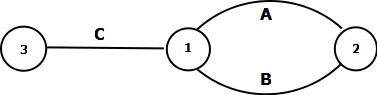
\includegraphics[scale=0.4]{final_images/Diagram3node.png}
%\end{center}
%	  \caption{Three Node Network}
%	\label{fig:3node} 
%%\vspace{0.1in}
%\end{figure}

% point: location diveristy makes TE difficult by changing TM; it is even difficult to estimate the traffic matrix after TE since 

The objective of TE is to ensure the the link utilization in the network is at minimal level but location can alter its effects by chanigng the traffic matrix and hence the utilization of links in the network.

\textbf{explain conditions}
We explain it using the three node netowrk in Figure~\ref{fig:3node}.
All link have capacity of 100 units and a constant delay.  Link A has a very small delay compared to links B and C; both B and C have equal delay. Node 1 has 100 units of demand which it can route from 2 as well as 3. In addition there is 20 units of demand at node 1 which it routes from 2. We assume that that the aggregate flow at a node constitutes of infinitesimal flows which can be split among multiple source locations. Similar to parallel TCP behavior, the ratio in which flows are split among multiple locations is inversely proportional to delay from a location. The routing in network is shortest path routing based on link weights and traffic is split equally among multiple path with equal weights.

\textbf{point: TE cannot be achieved since adaptation changes TM.}
Initially, link weights of A, B and C as 3, 2, 1 respectively. The traffic between 1 and 2 is routed only using B. 1 splits its demand of 100 units equally among 2 and 3. Thus traffic on links is A = 0, B = 70, and C = 50. In the next step, to balance load between A and B both link are set equal weights.  Let see how parallel TCP connections would change our estimates of link utilization in this case. Assuming each infinitesimal flow uses only one of the two links A and B, 50 unit of demand at 1 is routed using links B and C, and equal amount using A an C. In addition, the 20 units of background traffic is split equally among links B and C.  Since A has a much smaller delay than C, 50 units of demand at 1 routed using A and C will flow entirely through A. The demand routed using B and C will be split equally among B and C respectively. Thus traffic on links is A = 60, B = 35, and C = 25 which is different from expected values of A = 35, B = 35, C = 50. Thus, location diversity makes TE difficult by changing the traffic matrix and changing expected link utilization.

\section{Experimental setup}
\label{sec:exp_setup}

In this section, we describe our experimental setup based on ns-2 used to compare TE schemes with respect to their impact on application performance. 
We chose ns-2 as it is well-suited for simulating thousands of flows in an ISP network at the packet level while also incorporating transport and application behavior in a fine-grained manner.

% Evaluating application performance accurately necessitates modeling application and transport behavior, especially their response to network characteristics, in a fine-grained manner. We chose ns-2 as the simulation platform as it is well-suited to simulate thousands of flows in an ISP network at the packet level while also incorporating transport and application behavior in a fine-grained manner.


%Below, we discuss (1) why this simulation infrastructure is necessary, (2)  how we simulate real traffic matrices using ns-2, and (3) the traffic engineering schemes, real ISP topologies, and real traffic matrices in our experiments.

%In this section we describe our ns-2 simulation infrastructure to compare application performance for traffic engineering methods. First we discuss why this simulation infrastructure is necessary,  next we explain how we simulate traffic matrices using ns-2, and then we describe the TE schemes we compare and the ISP topologies and traffic matrices in our simulation.

%Our goal is to study the impact of TE schemes on end-to-end application performance. TE impacts application performance in several ways. First, TE determines the utilization on backbone links in the network, which in turn influences the loss rate and queuing delay of those links. Second,  TE determines the route between PoPs in the network and thereby impacts path delays. These factors---propagation delay, queuing delay, and loss rate---primarily influence user-perceived application performance, e.g., the loss rate and path delay determines TCP performance as well as the quality of streaming applications.

% Evaluating application performance accurately necessitates modeling application and transport behavior, especially their response to network characteristics, in a fine-grained manner. We chose ns-2 as the simulation platform as it is well-suited to simulate thousands of flows in an ISP network at the packet level while also incorporating fine-transport and application behavior in a fine-grained manner.


%\label{fig:ISP_data}
%\begin{wrapfigure}[12]{r}{0.25\textwidth}\footnotesize
%  \begin{center}
%  \begin{tabular}{ p{0.7cm} | p{0.7cm} | p{0.8cm}  }
%\textbf{BW (Mbps)} &\textbf{US users \%}  & \textbf{Europe users \% } \\ \hline 
%0.25 & 4.9 &   1.5 \\
%2.0  & 38.1 & 26.2  \\
%5.0 & 32.4 & 57.8	\\
%10.0 & 20.0 & 14.5 \\
%20.0 & 4.6 & - \\
%  \end{tabular}
%  \end{center}
%  \caption{Bandwidth Distribution}
%\end{wrapfigure}
%\label{fig:bandwidth_distribution}

%in order to determine link utilization levels and evaluate cost functions based on them. But, these cost functions do not capture network wide application performance.  They can be biased by traffic on one or a few links and  do not take into account the path delay which is important for application performance.  Simulation is the simplest approach to get a reasonable estimate of application performance. Another approach we considered was using theoretical model e.g. fixed point \cite{fixedpoint} models for large number of network flows. Since these are theoretical models, they do contain modeling errors. Another reason, we excluded theoretical models is these models are  not well understood  for a network with multiple bottleneck links \cite{fixedpoint}. Since we use a simulation infrastructure, our experiments are prone to simulation errors. An even more accurate experiment would involve emulation ( e.g Emulab) or a  virtualized infrastructure (e.g. VINI \cite{VINI} ) but we restricted ourselves to doing ns-2 simulations because its ease of use enabled us to run large number of experiments.



\subsection{Simulating traffic matrices in ns-2}
\label{sec:sim_TM}

Figure~\ref{fig:simulation1} illustrates the experimental process. Each simulation has three inputs: (1) \textsl{ISP Topology} (2) a sequence of \textsl{File Arrivals} at each node based on the current \textsl{TM} (3) \textsl{Routing}, as computed using a \textsl{TE} scheme. %The slanted text refers to the corresponding block in Figure~\ref{fig:simulation1}.

We construct an ISP network topology from our dataset consisting of PoP-level ISP topology maps. PoPs are represented as nodes and links between these nodes are the backbone links of the ISP. Each PoP node has a number of users connected to it via separate access links. Each PoP node also has five server nodes connected to it via high capacity links that serve files to users. The number of user nodes in our simulation ranges from 300-6000 nodes and the capacity of backbone links varies from 50Mbps to 1Gbps.

\begin{figure}
 \begin{center}
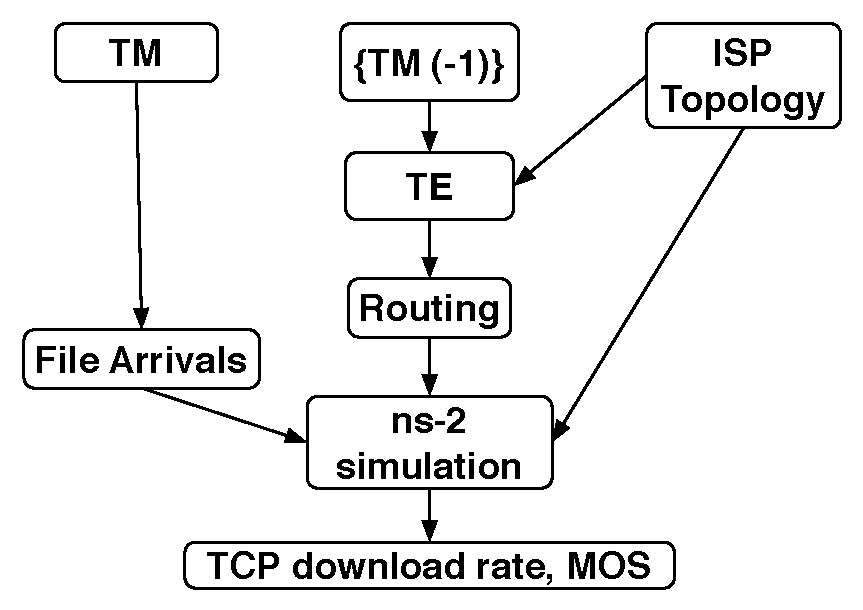
\includegraphics[scale=0.4]{final_images/Simulation1.pdf}
\caption{Block diagram of experiment process}
 \end{center}
 \label{fig:simulation1}
 \end{figure}
 
%\begin{figure}[tbh]
%  \begin{center}
%\includegraphics[scale=0.42]{}
% \end{center}
%\vspace{-0.1in}
%	  \caption{}
%  \label{fig:simulation1}
%\end{figure}

%\begin{figure}[tbh]
%  \begin{center}
%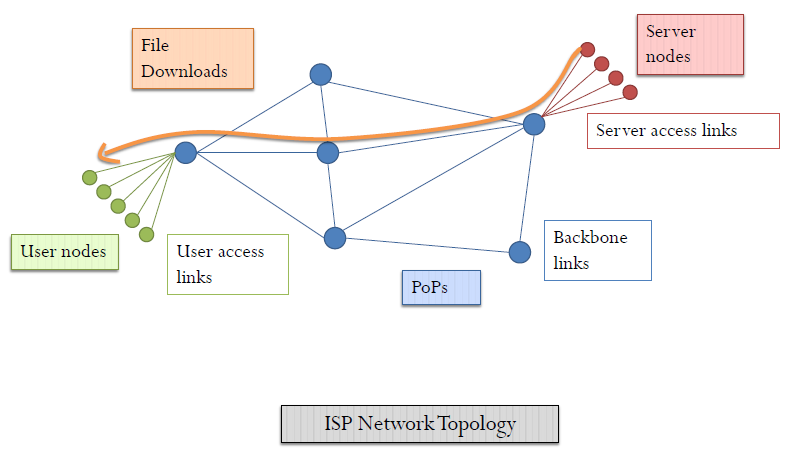
\includegraphics[scale=0.37]{final_images/expSetup.png}
% \end{center}
%\vspace{-0.1in}
%	  \caption{Diagram of an ISP network toplogy used in simulation}
%  \label{fig:isp_topology}
%\end{figure}


We translate a \textsl{TM} to a sequence of \textsl{File Arrivals} as follows. Suppose the traffic matrix entry from A to B is 100 Mbps and the duration being simulated is 200 seconds. During the experiment interval, we generate a sequences of file arrivals from A to B whose total size is 100Mbps $\times$ 200 seconds and the sizes are chosen from a realistic distribution.

A traffic engineering scheme \textsl{TE} calculates routing for \textsl{TM} based on a set of matrices \textsl{TM(-1)} which consists of either the current traffic matrix (for \opt) or a set of matrices from the previous traffic engineering {\em epoch} (for other TE schemes). The length of the epoch depends on {\em TE}, e.g., the epoch length for \optwt\  is 3 hours and for \cope\ is 1 day. When \textsl{TE}  yields a routing that splits flows across multiple paths between two nodes, the number of files assigned to each path is proportional to the flow along that path. We use  the source routing option in ns-2 to pin a file to a path. We note that the link utilization values obtained using this ns-2 methodology are consistent with those obtained using a simple linear program with the difference being at most 0.1.

%We are able to simulate matrices accurately using this method and the difference between empirical link utilization from ns-2 and the value obtained using a linear program based calculation is at most 0.1.

%We specify the path for each file using the source routing option in ns-2.


%\begin{table}[tb]\footnotesize
%    \subfigure[ISP Data]{\label{fig:ISP_data}
%  \begin{tabular}{ p{0.9cm} |  p{0.7cm} |  p{0.7cm} |   p{0.8cm} }
%\textbf{ISP} &\textbf{Nodes}  & \textbf{Links}  & \textbf{Duration of TM } \\ \hline
%US-ISP & 25 & 88 & 1hr\\ 
%Geant  & 22 & 68 & 15min \\
%Abilene & 12 & 30 & 5min	\\
%  \end{tabular}}
%    \subfigure[Bandwdith Distribution of Internet Users]{\label{fig:bandwidth_distribution}
%  \begin{tabular}{ p{0.7cm} | p{0.7cm} | p{0.8cm}  }
%\textbf{BW (Mbps)} &\textbf{US users \%}  & \textbf{Europe users \% } \\ \hline 
%0.25 & 4.9 &   1.5 \\
%2.0  & 38.1 & 26.2  \\
%5.0 & 32.4 & 57.8	\\
%10.0 & 20.0 & 14.5 \\
%20.0 & 4.6 & - \\
%  \end{tabular}}
%\caption{Simulation Data}
%\end{table}



In order to make the simulation complexity tractable, we scale down the topology and matrices.
ISP backbone link capacities run into tens of Gbps. Simulating such a network at scale even for 100 seconds would require sending data on the order of terabytes (or equivalently, a million 100KB files). Experimentally, we find that simulating at a tenth of this scale, i.e., 100K files, is feasible given the computational and memory constraints of our machines. A typical scale in our simulation is 1/20, i.e., we simulate the backbone link with 1/20 the capacity and also scale down the traffic between each source-destination pair accordingly.


%The scale of experiment determines the number of concurrent flows on a link. 

%A larger scale simulation has more concurrent flows in the network and makes the aggregate behavior more bursty.

\subsubsection{ISP topologies and traffic matrices}  We use datasets from the following three ISPs for our experiments:

\begin{figure*}\footnotesize
\begin{minipage}[b]{0.55\textwidth}
    \begin{tabular}{ l | c | c |   c }
%  \begin{tabular}{ p{0.9cm} |  p{0.7cm} |  p{0.7cm} |   p{1cm} }
\textbf{ISP} &\textbf{Nodes}  & \textbf{Links}  & \textbf{TM Duration} \\ \hline
Abilene & 12 & 30 & 5min	\\
&&&\\
Geant  & 22 & 68 & 15min \\
&&&\\
US-ISP & - & - & 1hr\\ 
  \end{tabular}
 \caption{ISP Data}
\label{fig:ISP_data}
\end{minipage}
\begin{minipage}[b]{0.45\textwidth}
  \begin{tabular}{ p{1.2cm} | p{1.5cm} | p{1.5cm}  }
\textbf{BW (Mbps)} &\textbf{US users \%}  & \textbf{Europe users \% } \\ \hline 
0.25 & 4.9 &   1.5 \\
2.0  & 38.1 & 26.2  \\
5.0 & 32.4 & 57.8	\\
10.0 & 20.0 & 14.5 \\
20.0 & 4.6 & - \\
  \end{tabular}
  \caption{Bandwidth Distribution}
\label{fig:bandwidth_distribution}
\end{minipage}
\end{figure*}

%
%\begin{figure}\footnotesize
%  \begin{center}
%    \begin{tabular}{ l | c | c |   c }
%%  \begin{tabular}{ p{0.9cm} |  p{0.7cm} |  p{0.7cm} |   p{1cm} }
%\textbf{ISP} &\textbf{Nodes}  & \textbf{Links}  & \textbf{TM Duration} \\ \hline
%Abilene & 12 & 30 & 5min	\\
%Geant  & 22 & 68 & 15min \\
%US-ISP & - & - & 1hr\\ 
%  \end{tabular}
% \caption{ISP Data}
%\label{fig:ISP_data}
%  \end{center}
%\end{figure}
%
%
%
%\begin{figure}\footnotesize
%  \begin{center}
%  \begin{tabular}{ p{1.2cm} | p{1.2cm} | p{0.8cm}  }
%\textbf{BW (Mbps)} &\textbf{US users \%}  & \textbf{Europe users \% } \\ \hline 
%0.25 & 4.9 &   1.5 \\
%2.0  & 38.1 & 26.2  \\
%5.0 & 32.4 & 57.8	\\
%10.0 & 20.0 & 14.5 \\
%20.0 & 4.6 & - \\
%  \end{tabular}
%  \end{center}
%  \caption{Bandwidth Distribution}
%\label{fig:bandwidth_distribution}
%\end{figure}
%


(1) \textbf{Abilene}, from the publicly available Abilene ISP data \cite{abilene}.
(2) \textbf{Geant}, the un-anonymized version of the Geant topology obtained from the TotemData \cite{TotemData} project personnel. 
(3) \textbf{US-ISP}, a large Tier-1 ISP topology obtained from authors of  \cite{MultiTM}.  TMs for all ISPs were logged in the period from 2004-2005. Figure \ref{fig:ISP_data} shows number of nodes, number of links, and the interval at which TMs are logged for each ISP.  The number of nodes and links for US-ISP is proprietary information.


%
%We used three datasets for our experiments as shown in Figure \ref{fig:ISP_data} and described below.
%
%\noindent\textbf{Abilene:} We used the publicly available Abilene ISP topology and traffic matrices \cite{AbileneData} logged once every 5 minutes.
%
%\noindent\textbf{Geant:} We used the Geant topology and TM data for the Geant network  provided by the Totem project \cite{TotemData}. We used the un-anonymized version of topology obtained from the project personnel. The matrices are logged once every 15 minutes. 
%
%\noindent\textbf{US-ISP:} We used the anonymized PoP level topology and traffic matrices from a US Tier-1 ISP (labeled as US-ISP throughout the paper) logged once every hour over from Feb13-Feb26, 2005. We obtained this data from the authors of \cite{MultiTM}.

%
%\begin{enumerate}
%\item \emph{Abilene}: We used the publicly available Abilene ISP topology and traffic matrices \cite{AbileneData} logged once every 5 minutes.
%\item  \emph{Geant}: We used the Geant topology and TM data for the Geant network  provided by the Totem project \cite{TotemData}. We used the un-anonymized version of topology obtained from the project personnel. The matrices are logged once every 15 minutes.
%\item  \emph{US-ISP}: We used the anonymized PoP level topology and traffic matrices from a US Tier-1 ISP (labeled as US-ISP throughout the paper) logged once every hour over from Feb13-Feb26, 2005. We obtained this data from the authors of \cite{MultiTM}. 
%\end{enumerate}
%
%\begin{figure}
%\begin{center}
%  \begin{tabular*}{0.35\textwidth}{@{\extracolsep{\fill}}| c | c | c |  c |}
%    \hline
%\textbf{ISP} &\textbf{\# Nodes}  & \textbf{\# Links}  & \textbf{TM Interval} \\ \hline \hline
%US-ISP & 25 & 88 & 1hr\\ \hline
%Geant  & 22 & 68 & 15min \\ \hline
%Abilene & 12 & 30 & 5min	\\ \hline
%  \end{tabular*}
%\caption{ ISP Data }
%\label{fig:ISP_data}
%\end{center}
%\end{figure}

\subsubsection{Simulation parameters}
Unless otherwise stated, we choose the following parameters for all of our simulations. Our goal is to choose parameters that are close to realistic values for ISPs.
% further discussion about the sensitivity of our results to the choice of these parameters is in Section~\ref{sec:discuss}.

\noindent\textbf{Scale:}  We experiment with Abilene, Geant and US-ISP datasets at  scales 1/10, 1/20 and 1/100 respectively. These are the largest scales we can experiment with for each network given our computational constraints.

\noindent\textbf{Duration:}  The simulation duration for most experiments is 300 seconds. We verified that running the simulations for longer durations did not qualitatively affect our results. Note that the duration here refers to the real time being simulated in ns-2, not the system time required to run the simulation.


\noindent\textbf{Bandwidth of users:} We use the bandwidth distribution of Internet users from the  ``State of the Internet Report'' \cite{Akamai-soti} released by Akamai, one of the largest commercial content distribution networks in operation today. Figure \ref{fig:bandwidth_distribution} tabulates this data for US and Europe.

\noindent\textbf{File sizes:} We simulate three file sizes of 100KB, 1MB and 10MB respectively contributing to  8\%, 3\% and 89\% of the total traffic respectively. These values are the fractions of traffic due to small files ($<$200KB), medium size files (200KB to 2MB), and large files ($>$2MB) in the Internet. We obtained these numbers by collating data from multiple sources \cite{urlinternet,kazaa,youtubestudy,pareto}.

%Typically, the average size of web files is less than 10KB, but we used a smallest file size of 100KB to limit the number of files in the simulation. The download rate of 100KB files using TCP is more sensitive to RTT since they may complete download even in slow start phase.
%Since we measure download rate of files, 10MB files would have similar file download rates as larger files

\noindent\textbf{Link delay:} We calculate the propagation delay of backbone links from geographic distances between nodes for Geant and US-ISP. For Abilene, we measure the propagation delay of backbone links using \emph{traceroute} and \emph{ping} between PlanetLab \cite{Planetlab} nodes in cities where the PoPs are located. All links use drop-tail queuing.

%\noindent\textbf{Queuing:} We have used Drop Tail queuing at all links.

\noindent\textbf{File inter-arrival time:} We  assume an exponential distribution of file inter-arrival times.


%\noindent\textbf{Router Buffer Size:} We set the router buffer sizes at the access and backbone links to the average bandwidth-delay product \cite{routerbuffersize} which is still widely used in production networks \cite{ExpRouterBuffer}. We defer further investigation of the impact of smaller router buffer sizes  \cite{routerbuffersize} to future work.  
% on the interaction between TE schemes and application performance

%\noindent\textbf{Link queue capacity:} We set the router buffer sizes at the access and backbone links to the average bandwidth-delay product \cite{routerbuffersize}. We note that although proposals for significantly smaller buffer sizes have been experimentally verified for backbone links networks \cite{ExpRouterBuffer}, this rule of thumb is still widely reflected in routers deployed in production networks \cite{ExpRouterBuffer}. We defer further investigation of the impact of smaller buffer sizes on the interaction between TE schemes and application performance to future work.

\subsubsection{Computational resources}
We use a shared cluster of 60 machines. Each machine has a 8-Core Intel Xeon processor and 16GB of memory. Each ns-2 simulation consists of 300--500s of simulated time and 10K to 200K file downloads, which results in a memory footprint of up to 10GB and takes between 1 to 48 hours to complete.

\subsection{Traffic engineering schemes} We select a subset of TE schemes reflecting a variety of proposed approaches in the literature including optimal TE (\opt), demand-oblivious TE (\invcap) and demand-aware TE (\optwt, \mplsavg\ and \cope).

{\bf{\opt}}, the minimum MLU TE scheme for a TM. We consider it as being representative of {\em online} TE schemes.

%a TE scheme that minimizes the maximum link utilization (MLU) for a given traffic matrix. We consider it as being representative of online TE schemes.

{\bf{\invcap}}, a simple routing scheme that does not ``engineer'' traffic, but instead  simply relies on shortest-path routing using the inverse of the link capacity as the link weight. \invcap\ is a common default routing protocol supported by popular commercial router vendors \cite{InvCapCite}.

{\bf{\optwt}},  a shortest-path routing algorithm using link weights computed using a heuristic algorithm to optimize a cost function \cite{fortz2000internet}. We use its implementation in the Totem Toolbox \cite{TotemData}. Typically, ISPs recompute routes a few times a day based on a set of measured TMs, so we simulate \optwt\ by computing a new routing every 3 hours based on the average of matrices in the past 3 hours.

%a TE scheme widely used by ISPs\cite{FortzThorup2} that engineers link weights for a given traffic matrix (TM) such that shortest-path routing using those weights for that matrix minimizes a specific cost function. Typically, ISPs recompute routing a few times a day based on a set of measured TMs, so we simulate \optwt\ by computing a new routing every 3 hours based on the average of matrices in the past 3 hours.  We use the implementation of the Fortz-Thorup algorithm available in the TOTEM toolbox \cite{TotemData} to compute the optimal link weights for a TM. This algorithm minimizes a convex cost function based on link utilization described in \cite{FortzThorup} and used in several follow-on papers.

{\bf{\mplsavg}}, a TE scheme that minimizes the MLU in an {\em offline} manner. Similar to \optwt, \mplsavg\ recomputes a new routing once every 3 hours based on average of TMs in past 3 hours.

%Unlike \opt\ above that uses the most recent matrix to recompute routing frequently (on the order of minutes), \mplsavg\  computes a routing so as to minimize the MLU for a matrix averaged over the past 3 hours TMs.

{\bf{\cope}}, a TE scheme that minimizes the common-case MLU while limiting the worst-case MLU caused by unpredictable spikes in the traffic matrix. We use the authors' implementation and parameters settings, and recompute routes once a day based on the previous day's TMs  as in \cite{COPE}.


{\bf{\mindelay}} scheme minimizes average latency for all traffic, unlike the schemes above which optimize link utilization based metrics.
Specifically, the objective function \mindelay\ optimizes is $\sum_{e \in E} d_e T_e$, where $E$  is the set of all links, $d_e$ is the propagation delay of link $e \in E$, and $T_e$ is the total traffic (in bits/sec) for $e\in E$. 
We evaluate \mindelay\ to answer whether user-perceived performance improves if we optimize latency instead of MLU.
We constrain the linear program so that MLU does not exceed 0.6, thereby ensuring that high link utilization does not hurt user-perceived  performance.
Like \opt, \mindelay\ has perfect knowledge of traffic matrix.


%\noindent{\bf{\cope}}, a TE scheme that seeks to minimize the MLU while limiting the worst-case link utilization caused by unpredictable spikes in the traffic matrix. As described in the paper \cite{COPE1}, COPE recomputes routing once a day so as to minimize the MLU for a matrix that is averaged over matrices observed during the previous day while limiting the worst-case link utilization resulting from any matrix lying within the convex hull of matrices observed during the previous day. We obtained the code for COPE from the authors and used their parameter settings throughout our experiments.
  
% COPE's optimization formulation optimizes measured traffic matrices and limits worst case link utilization during unpredictable spikes in traffic. We compute a new routing once every day as in the paper\cite{COPE1}. The performance ratio parameter is set to 2.2. We use the authors' code for experiments. 







\begin{figure*}[tbh]
  \begin{center}
%    \subfigure[Mean download rate]{\label{fig:allisps_mean_throughputs}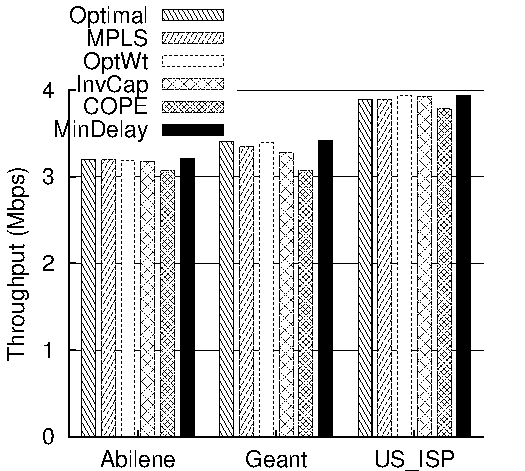
\includegraphics[width=35mm,height=30mm]{final_images/mean_throughput_hist_plot.pdf}}
    \subfigure{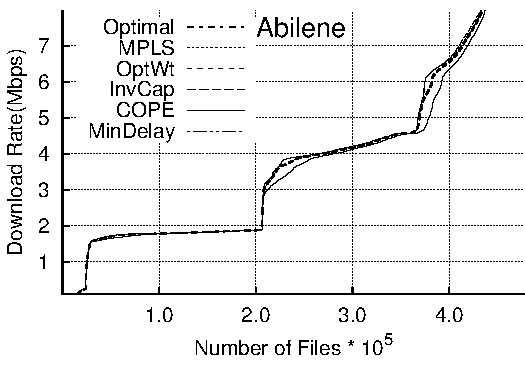
\includegraphics[scale=0.55]{final_images/G3_CDF/Abilene_download_rates_aggregate_plot.pdf}}
    \subfigure{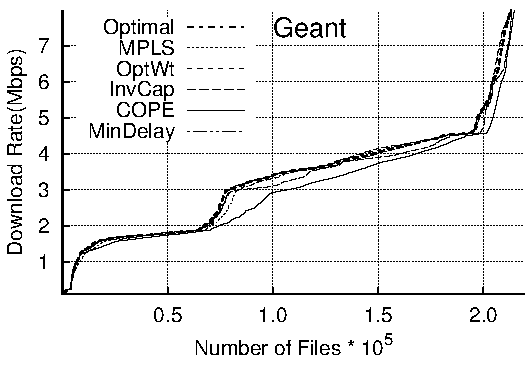
\includegraphics[scale=0.55]{final_images/G3_CDF/Geant_download_rates_aggregate_plot.pdf}}
    \subfigure{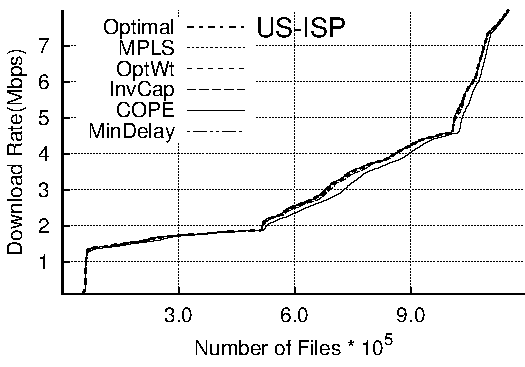
\includegraphics[scale=0.55]{final_images/G3_CDF/ATT_download_rates_aggregate_plot.pdf}}

  \end{center} 
  \caption{Download rate CDFs for all TE schemes are near identical except \cope\ which has slightly lower performance}
  \label{fig:throughputs_CDF}
\end{figure*}

\section{User-perceived performance}
\label{sec:app_performance}
In this section, we present a comparative analysis of the impact of different TE schemes on user-perceived performance. A summary of our findings is as follows. First, all TE schemes  including \invcap\ show nearly identical user-perceived performance for TCP and UDP traffic. Second, different TE schemes do achieve different MLUs as expected, suggesting that MLU is a poor predictor of user-perceived performance. Third, COPE consistently performs slightly worse than all other schemes in TCP throughput, suggesting that accounting for unpredictable variations in traffic hurts the common case user-perceived performance.

%we present our comparison of traffic engineering schemes based on simulation of traffic matrices at Internet loads for 3 ISPs. Our simulation shows that unexpectedly that all traffic engineering schemes (even \invcap) perform near identical in terms of download rates using TCP for all ISPs. We also show that MLU a metric commonly used metric for traffic engineering does not predict TCP throughput well and traffic engineering which optimizes for unexpected traffic variations increases delay and hurts TCP throughput.

%In this section, we present our comparison of traffic engineering schemes based on simulation of traffic matrices at Internet loads for 3 ISPs. Our simulation shows that unexpectedly that all traffic engineering schemes (even \invcap) perform near identical in terms of download rates using TCP for all ISPs. We also show that MLU a metric commonly used metric for traffic engineering does not predict TCP throughput well and traffic engineering which optimizes for unexpected traffic variations increases delay and hurts TCP throughput.

%Prior works on traffic engineering have measured its performance using linear programming simulation and have used metrics such as the maximum link utilization or similar cost functions based on link utilization.


\subsection{TCP performance}

We simulate TMs from 2 days of data for each ISP. For each day, we simulated 50 matrices measured at 5-minute intervals for Abilene, 25 matrices measured at 15-minute intervals for Geant, and 24 matrices measured hourly for US-ISP. We present results for the second day. The metric of user-perceived performance is the \emph{download rate} of files using TCP, where the file arrival workload is generated using the traffic matrices as described in Section \ref{sec:sim_TM}.

%\begin{figure}
%\begin{center}
%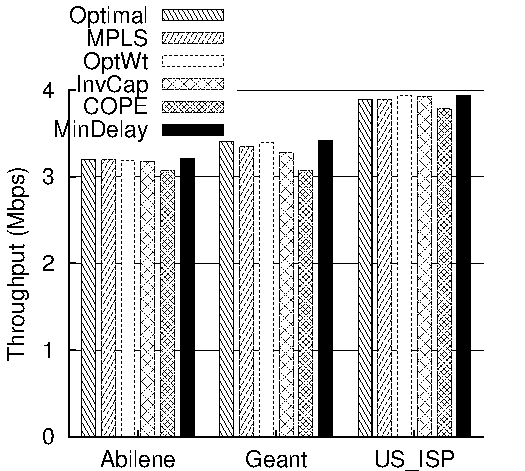
\includegraphics[scale=0.6]{final_images/mean_throughput_hist_plot.pdf}
%\caption{Mean download rates}
%\end{center}
%\label{fig:allisps_mean_throughputs}
%\end{figure}
%
%\begin{figure}
% \begin{center}
%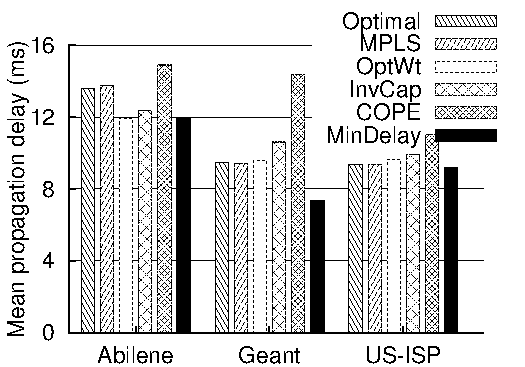
\includegraphics[scale=0.6]{final_images/G4_propdelay/mean_prop_delay_plot.pdf}
%\caption{COPE has the highest propagation delay among TE schemes}
% \end{center}
% \label{fig:prop_delay_all}
% \end{figure}


Figure \ref{fig:allisps_mean_throughputs} shows the mean download rate of files, where the average is across all files across all of the simulated matrices for each TE scheme.
We make three observations from this graph. 
First, all schemes achieve nearly same mean download rates with the exception of COPE that is consistently worse by up to  10\%.
Next, \opt\ (the leftmost bar in each group) is not always the best as minimizing MLU is not the same as optimizing TCP performance.
Finally,  \mindelay\ (the leftmost bar in each group) that optimizes latency performs the same as other TE schemes that optimize link utilization based metrics.


Figure \ref{fig:throughputs_CDF} shows the corresponding CDFs for the mean download rates in Figure \ref{fig:allisps_mean_throughputs}. The CDFs show that the near-identical TCP performance achieved by all TE schemes is not an artifact of presenting a specific statistic such as the mean, but is reflected by the entire distribution.  All distributions show a stepwise increase which suggests that access links are a bottleneck for a significant fraction of file transfers. This observation partly explains why \mindelay\ fails to  improve TCP throughput over other schemes: TCP throughput cannot be improved for flows bottlenecked at access link even if \mindelay\ scheme reduced the RTT for these flows.

\begin{figure*}[t]
\begin{minipage}{0.45\textwidth}
\includegraphics[scale=0.6]{final_images/mean_throughput_hist_plot.pdf}
\caption{Mean download rates}
\label{fig:allisps_mean_throughputs}
\end{minipage}
\hspace{1cm}
\begin{minipage}{0.45\textwidth}
\includegraphics[scale=0.6]{final_images/G4_propdelay/mean_prop_delay_plot.pdf}
\caption{COPE has the highest propagation delay among TE schemes}
 \label{fig:prop_delay_all}
\end{minipage}
\end{figure*}

% we present the download rate of all files from all traffic matrices during the day sorted in increasing order  and in Figure ~\ref{fig:allisps_mean_throughputs} we show the mean value of the above distribution.

%What is result ?
%The download rate curves for all traffic engineering schemes are strikingly similar for all the topologies. Even the simple routing scheme, \invcap{}  has mean and median throughputs within 5\% of \opt{}  for all 3 topologies.  \opt{} does not have any additional gain over other routing schemes in download rate. The only notable difference is throughput is for \cope{} which has up to 10\% lower median throughput than \opt{} for Geant toplogy and has lowest throughput among all schemes. All 3 graphs show a step-wise increase which shows that access link are bottleneck for a significant fraction of file transfers.


%
%\begin{figure}[htb]
%  \begin{center}
%\includegraphics[scale=0.5]{final_images/mean_throughput_hist_plot.pdf}
% \end{center}
%	  \caption{Mean download rates of files for Internet traffic matrices}
%  \label{fig:allisps_mean_throughputs}
%\end{figure}




%\begin{figure*}[tbh]
%  \begin{center}
%%    \subfigure[Mean download rate]{\label{fig:allisps_mean_throughputs}\includegraphics[width=35mm,height=30mm]{final_images/mean_throughput_hist_plot.pdf}}
%    \subfigure[Download rate CDF Abilene]{\includegraphics[scale=0.6]{final_images/G3_CDF/Abilene_download_rates_aggregate_plot.pdf}}
%    \subfigure[Download rate CDF Geant]{\includegraphics[scale=0.6]{final_images/G3_CDF/Geant_download_rates_aggregate_plot.pdf}}
%    \subfigure[Download rate CDF US-ISP]{\includegraphics[scale=0.6]{final_images/G3_CDF/ATT_download_rates_aggregate_plot.pdf}}
%  \caption{Download rate CDFs for all TE schmes are near identical except \cope\ which has slightly lower performance}
%  \label{fig:throughputs_CDF}
%  \end{center} 
%\vspace{-0.2in}
%\end{figure*}

%\subsection{Analysis}
%Here, we present an analysis of above results using additional statistics measured from simulation.

\subsubsection{MLU vs. TCP performance}

To further investigate the results in Figure \ref{fig:allisps_mean_throughputs} and Figure \ref{fig:throughputs_CDF}, we analyze the empirically observed MLU for all TE schemes in the experiments. Figure \ref{fig:All_ISPs_MLU} plots the MLUs for all matrices considered. For US-ISP the MLU data is proprietary, so we present the ratio of MLU with respect to \opt. As expected, different TE schemes do show substantially different MLUs. For example, the MLU for \invcap\ and \optwt\ is up to twice the MLU of \opt\ in some cases; \mindelay\ has a MLU of 0.6 on Geant, which is more than twice of \opt's MLU. These results suggest that MLU is a poor predictor of download rate performance: schemes with near-identical TCP throughput have very different MLUs, and COPE despite achieving near-optimal MLU consistently shows sub-optimal TCP throughput.

%\textbf{MLU:}
%The above results may seem surprising if we observe the empirical MLU of all the traffic matrices simulated (Figure ~\ref{fig:All_ISPs_MLU}). The graphs show a significant difference among traffic engineering schemes. MLU for \invcap{} or \optwt{} is up to twice the MLU of \opt{} in many cases. The contrast between MLU and download rate graphs leads us to the conclusion that a higher MLU for Internet traffic matrices does not imply a worse TCP performance. We observe that \cope{} has a MLU close to \opt{} in Geant and US-ISP topologies but its download rate is lower than all other TE schemes. This is because \cope{} has greater path delay. This shows that even a low MLU traffic engineering scheme can have a worse TCP performance.

The main reason why MLU does not affect download rate is because queuing delay and loss rates are negligible until link utilization reaches a threshold. In our experiments, link utilization below 0.7 causes near negligible loss rates and queuing delays. Since the MLUs on most of the traffic matrices are below this value, loss rates on backbone links minimally impact the throughput of file downloads.  These observations are consistent with a recent  study on Level-3 ISP network  \cite{ExpRouterBuffer} showing that loss rates on backbone links are zero even at 95\%  link utilization. This threshold is expected to be higher for actual backbone traffic as our experiments are at scale 1/10 or smaller. At larger scales, there would be more concurrent flows resulting in less bursty traffic and lower loss rates.

%The main reason why MLU does not affect download rate is because queuing delay and loss rates are negligible until link utilization reaches a threshold. We observe this in our simulation and this phenomenon has also been observed for backbone traffic in the Internet \cite{ExpRouterBuffer}. Since the MLUs on most of the traffic matrices are below this threshold, loss rates on backbone links minimally impact the throughput of file downloads.  These observations are consistent with a recent study on Level-3 network\cite{ExpRouterBuffer} showing that loss rates on backbone links are zero even at 95\%  link utilization. In our simulations, the threshold at which links exhibit non-negligible loss is around 0.7. This threshold is expected to be higher for actual backbone traffic as our experiments are at scale 1/10 or smaller. At larger scales, there would be more concurrent flows resulting in less bursty traffic and lower loss rates.


The second reason why MLU hardly impacts the average download rate as well as the distribution is because it is largely determined by the traffic of only one link. Even under high MLU, the rest of the network may not be congested. File download rates are affected only for flows on this link, which may be a tiny fraction of the total traffic.




%There may exist intermittent traffic congestion which cause higher loss rates on backbone links. These happen due to interdomain routing changes \cite{BGPloss} (which are frequent) or due to anomalous traffic spikes in the Internet. An intradomain TE protocol cannot gurard against losses due to interdomain routing changes. It can be argued that doing \opt{} TE (using online traffic engineering) or a  TE scheme similar to \cope{} which is robust to traffic fluctuations would perform better in case of traffic spikes. These two routing schemes do not show any gain compared to other offline traffic engineering schemes in our experiment.  We infer that either these spikes are short enough to affect the average traffic matrices measured in our data set or the ISP networks are well provisioned to handle the spikes.


%\begin{figure}[tbh]
%  \begin{center}
%\includegraphics[scale=0.6]{final_images/G4_propdelay/i_o_diff_plot.pdf}
%  \end{center}
%  \caption{Propagation delay for Internet TMs.}
%  \label{fig:prop_delay_all}
%\end{figure}



\begin{figure*}[tb]

  \begin{center}
\subfigure{\includegraphics[scale=0.55]{final_images/G2_MLU//Abilene_MLUAverageUtilTable_plot.pdf}}
\subfigure{\includegraphics[scale=0.55]{final_images/G2_MLU//Geant_MLUAverageUtilTable_plot.pdf}}
\subfigure{\includegraphics[scale=0.55]{final_images/G2_MLU//ATT_MLUAverageUtilTable_plot.pdf}}
  \end{center}
  \caption{TE schemes differ as much as 2$\times$ in MLU}
  \label{fig:All_ISPs_MLU}
  \end{figure*}
  
  
 
%\begin{minipage}{1.9in}
%  \begin{center}
%\includegraphics[scale=0.6]{final_images/G4_propdelay/mean_prop_delay_plot.pdf}
%  \end{center}
%  \caption{}
%
%
%  \label{}
%\end{minipage}
%\vspace{-0.2in}


\subsubsection{The price of predictability}
Why is \cope's performance consistently worse than the other schemes? To investigate this, we analyzed the propagation delays of routes computed by COPE. Given uniformly low loss rates and queueing delays, propagation delays primarily determine TCP performance.

Figure \ref{fig:prop_delay_all} shows the path delay averaged across all files and across all matrices for the different TE schemes. \cope{} has a significantly higher delay compared to all other schemes. We attribute this phenomenon to \cope{}'s optimization approach, which engineers for unpredictable spikes in traffic demands. Specifically, \cope\ attempts to bound the worst-case MLU for any traffic matrix similar to oblivious routing like schemes \cite{Cohen}. \cope\ intentionally routes some traffic along longer paths so as to leave room for occasional traffic spikes along shorter paths. While this approach makes \cope\ robust with respect to MLU under rare spikes in traffic, it comes at the cost of hurting common-case user-perceived performance.  Although we have not experimented with other oblivious routing schemes, these results suggest that any oblivious routing scheme that attempts to optimize MLU, e.g., \cite{Cohen}, is likely to incur a similar penalty in  user-perceived performance in the common case. 

%Although prior work has recognized that TE schemes can increase path delay, e.g.. \cite{TeXCP06}, to the best of our knowledge, our work is the first to empirically quantify the impact on TCP throughput and to show that engineering for rare traffic spikes comes at the cost of hurting common-case TCP throughput.

%It is known that TE schemes can increase path delay \cite{TeXCP06}. Our contributions are to show that \cope\ has a significantly higher path delay than other TE schemes and  to accurately measure the impact of increased path delay on TCP throughput. 


%This statistic explains why \cope{} has the lowest download rate among all schemes for Geant and US-ISP topologies. Our finding also suggests that other oblivious routing schemes which optimize for MLU \cite{ObliviousRouting} may have lower TCP throughput.

%We infer that the robustness of \cope to unpredictable traffic spikes comes at the cost of higher path delay and reduced TCP througput.  


%We observe that in Geant and US-ISP topologies \cope has lower mean and median value than other schemes. It is because the routing computed by \cope has a higher path delay compared to other traffic engineering schemes. We show the average propagation delay for all TE schemes in ~\ref{fig:prop_delay_all}. This statistic is the average of propagation delay of each file in our simulation. Different routings have same file request sequence but their paths depend on the routing. All TE schemes except \cope have similar path delay. The higher delay is significant for Geant and US-ISP topologies which explains its lower throughput. 

%\textbf{Users' Access Link Capacity:}

%Access link capacity is the  bottleneck for majority of file downloads in Figure ~\ref{fig:throughputs_CDF} but this may not hold true in Internet. The reasons are that paths have more delay (e.g. intercontinenal links), the access link at the server may be a bottleneck. Both these observations  affect all TE schemes identically and are unlikely to affect our findings. 

%It may be argued that our findings would not hold if Internet users had higher access link capacities. To verify this hypothesis, we also performed experiments where users access links had twice the current access link capacities. Our results remained unchanged  \cite{TechReport}.


%The minimum value of download rate in Figure ~\ref{fig:throughputs_CDF} is near zero in our simulation. This is because of congestion at the access link of users. In some cases a new file download starts on the same user node before previous download has finished. The previous flow has a large window size and sends many more packets than the new flow. In some cases, this causes multiple packet losses	 at access link queue for the new flow. Repeated timeouts due to these loss result in near zero download rates for some files. 

% Summary of result
%In this section we presented our comparison of traffic engineering schemes for file download rates in Internet. Our novel simulation based comparison has following main results: (1) All traffic engineering schemes (even \invcap{}) performs near identical in file download rate for Internet traffic matrices. (2) MLU is a poor predictor of TCP throughput : \invcap{} which has 2x higher MLU than \opt has nearly the same throughput and \cope{}'s MLU is near optimal but its throughput is lowest. (3) A traffic engineering approach such as \cope{} which engineers for unpredictable traffic demands increases path delay and reduces TCP throughput.

\subsection{UDP performance}
\label{sec:UDP_perf}
\subsubsection{Measuring UDP performance}

We assume that the loss rate and the queuing delay on each link for UDP traffic is the same as that measured during experiments with TCP traffic. This assumption is reasonable as TCP accounts for over 90\% of Internet traffic \cite{SprintBackbone}. We calculate the loss rate and delay for a path by combining the loss rates of links along the path; we compute the delay by summing the propagation and queuing delay of links along the path.

We compare performance of VoIP traffic (which uses UDP) using Mean Opinion Score (MOS). MOS is an industry standard VoIP call quality metric for which a score of above 4 is considered good and below 3 is considered bad. We calculate MOS using the formula in \cite{MOS-formula}  which calculates MOS given the loss rate and delay for a path. 

We calculate MOS for VoIP calls between all pairs of source and destination PoP nodes in an ISP. First, we measure loss rates and queuing delay on backbone links for each 10-second interval.  For each interval, we calculate the MOS for a path based on its end-to-end loss rate and delay. The mean MOS for a path is the average value of MOS over all intervals. For TE schemes that split traffic across multiple paths between a source-destination pair, the mean MOS for a source-destination node pair is calculated as the weighted average of mean MOS weighted by the fraction of the traffic split along each path between the node pair. We similarly calculate the 5th percentile MOS for a source-destination pair by taking the weighted average of 5th percentile MOS values for all its paths.

\subsubsection{Results}
We obtain a distribution of mean MOS values for a TE scheme by combining mean MOS values for all pairs of source and destination nodes for all traffic matrices. We find that the minimum and the maximum values of mean MOS for all TE schemes are in the range (4.08, 4.14) for Abilene, (4.07, 4.14) for Geant and (4.08, 4.14) for US-ISP.  The range of values for 5th percentile MOS are (4.07, 4.13) for Abilene, (4.08, 4.14) for Geant and (4.05, 4.14) for US-ISP. MOS scores for all schemes are always above 4.0 and the differences between different TE schemes is at most 0.1. These results are not surprising since loss rates and queuing delay are near-negligible for most links in the network. Furthermore, MOS is not very sensitive to few milliseconds difference in propagation delay among TE schemes.




%\tbd{In summary, our study of the impact of state-of-the-art TE schemes on application performance reveals the following. All TE schemes have near-identical TCP throughput and UDP performance for a VoIP call quality metric. }

	


%The only exception is \cope\ that has a slightly lower TCP throughput, which is because it attempts to absorb unpredictable variations in traffic at the cost of common case application performance. Furthermore, we find that the commonly used MLU metric is a poor predictor of TCP performance. Taken together, these results suggest that the simplest routing scheme, \invcap, suffices to achieve similar performance as sophisticated traffic engineering schemes proposed in the literature or in use in production networks today.

%Our experiments in this section showed that all traffic engineering schemes perform near identical in terms of TCP throughput for traffic matrices from 3 ISPs in the Internet. Even though traffic engineering schemes differ by as much as twice in terms of MLU, their TCP throughput is identical because of near zero loss rates and queuing delay on most links. An interesting observation is that \cope which has MLU close to \opt has a lower TCP throughput.

%In the following section, we experiment with traffic matrices at higher load than current Internet and study the effect of application adaptation.


%In FIgure ~\ref{fig:All_ISPs_MLU} we show the maximum link utlization for the traffic matrices we experiment with. The graphs show a significant difference among traffic engineering schemes. MLU for \invcap or \optwt being upto twice the MLU of \opt but these differences are not reflected in throughputs. Higher link utliizations cause increased loss rates and higher queuing delay for packets. We find that in our experiments both these values remain near-zero until link utilization values of 0.6 in our experiments. Since the MLU on most of the traffic matrices are below this threshold value, MLU isnt a factor in the throughput of file downloads. Even if the utilization on one link is high enough to increase loss rates on that link the rest of the network may not be facing any congestion. File downloads rates are affected only for flows on this link, which could a small fraction of total traffic.


%In Fig ~\ref{fig:allisps_aggregate_InternetBW}, we also show the CDF of TCP throughput for all files for US-ISP topology . This shows that access link is the bottleneck for a large fraction of file transfers in our simulation. This helps us explain the near identical values for all routings. This observation is likely to be different for internet since paths have more delay (e.g. intercontinenal links ), the access link at the server may be a bottleneck, and there may exist intermittent traffic congestion which cause higher loss rates on backbone links. The first two reasons affect all TE schemes identically and are unlikely to affect our findings. The third reason intermittent congestion on backbone in internet can happen beacuse of interdomain routing changes [cite sprint study] ( which are frequent ) or due to anomalous traffic spikes in the internet. An intra domain TE protocol cannot gurard against losses due to interdomain routing changes. It can be argued that doing \opt TE ( using online traffic engineering ) or a  TE scheme similar to \cope which is robust to traffic fluctuations would perform better in case of traffic spikes. Since these two routing schemes do not show an improvement compared to other offline traffic engineering schemes, either these spikes are short enough to affect the average traffic matrix over 15 min or 1 hour period or the spikes do not cause performance degradation for internet traffic matrices for all TE schemes.


%It must be noted that our experiments are at scale 1:10 to 1:50. At, higher scale the loss rate and queuing delay would be lower at the same link utilization level. As scale increases, the router buffer sizes increase and the per packet processing time decrease proportionally. If we take the analogy from a queuing model such as $M/M/1/K$ queue, at higher loads the mean packet arrival rate ($\lambda$), the mean packet processing rate($\mu$) and the capacity of the queue ($K$) increase proportionately. The formula for loss rates of this queuing model show that both these metrics decrase as $\lambda$, $\mu$  and $K$ increase proportioately \cite{queue}. If anything , the scale of our experiments reinforces our results that MLU has minimal application performance in realistic ISP topologies. 


%\subsubsection{Comparison of path delay}
%
%In Fig ~\ref{fig:prop_delay_all}, we present the average propagation delay for TE methods. The propagation delays presented are the average propagation delay for all file transfers.  The notable outlier in the table is \cope which has the highest delay in all three topologies. It delay is maximum in Geant where it has 25\% higher delay than the next highest delay TE method. This explains the the reason for \cope having lower throughput than other TE schemes. All other TE methods have delay within 1ms of each other for Abilene and US-ISP. Their near identical througputs reflect this trend.
%
%We calculate this statistic from the traffic matrix and routing computed by a TE method. First, we calculate the delay of tranfers between a source destination pair by multiplying the propagation delay by the total traffic on each path. The sum of this delay for all source destination pairs gives the total delay for a traffic matrix. The total propagation delay is the sum of delays of all trafic matrices divided by the sum of all traffic matrices.


%
%\begin{figure}
%\begin{center}
%  \begin{tabular}{| l | c | c | c | }
%    \hline
%Routing & Abilene & Geant & US-ISP \\ \hline \hline
%\opt &  4.54 &	9.46 & 9.37\\ \hline
%\invcap & 4.13 &10.62 & 9.90 \\ \hline
%\mplsavg & 4.58 & 9.40 & 9.37\\ \hline
%\cope &4.97 & 14.38 & 11.03\\ \hline
%\optwt & 3.98 & 9.57 & 9.64\\ \hline
%MinDelay & 3.97 & 7.34 & 9.21\\ \hline
%  \end{tabular}
%\caption{Propagation delay (in ms) for TE methods on different topologies}
%\end{center}
%\label{fig:prop_delay_all}
%\end{figure}

%\subsection{Effect of access link bottlenecks}
%
%We measure the effect of access link capcity of users on our results by experimenting at higher capacity access link bottlenecks. A reasonable choice for higher access link bottleneck is doubling current the access link capacities. In Table ~\ref{fig:all_isps_internetBWx2} shows the mean throughputs for all 3 ISPs. The mean throghputs increase by 1.3-1.7 times but the relative difference between different routings remain the same. This shows that throughputs of different traffic engineering schmes are near identical because of current traffic load in the network and would remain identical even if the current internet bandwidths were much higher.
%
%\begin{figure}[tbh]
%  \begin{center}
%\includegraphics[scale=0.7]{newImages/mean_throughput_twice_internetBW.jpg}
%  \end{center}
%  \caption{Mean throughputs of file transfers at twice internet access link bandwidths}
%  \label{fig:all_isps_internetBWx2}
%\end{figure}

%\begin{figure}
%\begin{center}
%  \begin{tabular}{| l | c | c | c | }
%\hline
%Routing & Abilene & Geant & US-ISP \\ \hline \hline			
%\opt	&	589.5	&	720.6	&	671.1	\\ \hline
%\\invcap	&	580.6	&	721.9	&	640.1	\\ \hline
%\mplsavg	&	589.4	&	720.0	&	654.1	\\ \hline
%\cope	&	560.4	&	695.4	&	587.8	\\ \hline
%\optwt	&	586.2	&	723.1	&	662.2	\\ \hline
%MinDelay	&	589.8	&	723.9	&	663.9	\\ \hline
%  \end{tabular}
%\caption{Mean throughputs at twice the internet access link bottlenecks}
%\end{center}
%\label{fig:all_isps_internetBWx2}
%\end{figure}

%\begin{figure*}[htb]
%  \begin{center}
%    \subfigure[Download rate US-ISP]{\label{fig:edge-a}\includegraphics[scale=0.4]{newImages/US_ISP/internetBW_scale2/download_rates_aggregate_plot.pdf}} 
%    \subfigure[Download rate Geant ISP]{\label{fig:edge-a}\includegraphics[scale=0.4]{newImages/Geant/internetBW_scale2/download_rates_aggregate_plot.pdf}} 
%    \subfigure[Download rate Abilene ISP]{\label{fig:edge-a}\includegraphics[scale=0.4]{newImages/Abilene/internetBW_scale2/download_rates_aggregate_plot.pdf}}  
%    \subfigure[Download ratio US-ISP]{\label{fig:edge-b}\includegraphics[scale=0.4]{newImages/US_ISP/internetBW_scale2/opt_download_ratios_aggregate_plot.pdf}} 
%    \subfigure[Download ratio Geant ISP]{\label{fig:edge-b}\includegraphics[scale=0.4]{newImages/Geant/internetBW_scale2/opt_download_ratios_aggregate_plot.pdf}} 
%    \subfigure[Download ratio Abilene ISP]{\label{fig:edge-b}\includegraphics[scale=0.4]{newImages/Abilene/internetBW_scale2/opt_download_ratios_aggregate_plot.pdf}} 
%  \caption{US Tier 1 ISP, Aggregate performance on 1 day traffic matrices,twice today's internet access link bottleneck distribution }
%  \end{center}
%  \label{fig:allisps_aggregate_internetBWX2}
%\end{figure*}

%As an interesting aside, we present the results for no access link bottlenecks in Fig  ~\ref{fig:allisps_aggregate_nolimit} .
%
%\begin{figure*}[htb]
%  \begin{center}
%\subfigure[US-ISP]{\label{fig:edge-c}\includegraphics[scale=0.75]{newImages/ATT_nolimit_Download_ratio_aggregate_plot.pdf}}
%\subfigure[Geant]{\label{fig:edge-c}\includegraphics[scale=0.75]{newImages/Geant_nolimit_Download_ratio_aggregate_plot.pdf}}
%\subfigure[Abilene]{\label{fig:edge-c}\includegraphics[scale=0.75]{newImages/Abilene_nolimit_Download_ratio_aggregate_plot.pdf}}
%  \end{center}
%  \caption{All ISPs : Download ratios for 1 day traffic matrices, without access link bottlenecks}
%  \label{fig:allisps_aggregate_nolimit}
%\end{figure*}

%\subsection{Experiments at higher scale}
%As said previously in this section, our simulations at lower scale provide a more challenging environment for comparison. To experimentally validate our findings at a higher scale, we selected 5 traffic matrices from each ISP and repeated our simulation at a higher scale. We simulated Abilene and Geant topology at original scale and the US-ISP topology at scale 1:10. We present the aggregate download ratios for 5 traffic matrices for at scale 1:50 and scale 1:10. The download ratios curve highlight the difference between traffic engineering schmes more clearly. The shape of the curves look almost the same in both graphs. This shows that our results remain consistent even at higher scale.
%
%Thus our results for 3 ISPs based on ns-2 simulations show that under traffic conditions in the internet the throughput performance of all traffic engineering schemes differ are near identical. Our results are consistent even at higher acess link botttlenecks in the internet and on experiment at higher scale. These findings show that difference in MLU for TE schemes does not translate to an improvement in throughput in internet conditions. Propagation delay is a more important factor and traffic engineering schemes which increase propagation delay have lower throughputs. 

%
%\subsection{Application Performance at higher loads}
%
%\subsubsection{Single Download Location}
%
%\subsubsection{Multiple Download Downloads}

\section{Capacity and location diversity}
\label{sec:capacity}
%things to do to ready  section 5

%A. Relative Input-Output Difference
%	- Rewrite example
%	- update y-axis \maxiodiff{} on graph, update caption 
%	- Write formal proof

%B. Simulating application adaptation ..
%	- improve writing

%C. Experimental procedure
%	- make changes suggested by Aditya

%D. Capacity increase with location diversity
%	
%	1. LP:

%	- finish writing
%	- update graphs
%	- check values
%	- update linear program in appendix
%	
%	2. ns-2 simulations:
%	
%	- update data based on simulations
%	- calculate confidence intervals
%	- replot graphs
%	- rewrite results

%E. Capacity increase with fraction of location diversity traffic
%	- get data in new format
%	- plot graph in gnuplot
%	- write subsection

%F. Write summary paragraph

%\textbf{intro to section}




%The results in the previous section show that different TE schemes yield nearly identical application performance at traffic demands encountered today. In this section, we compare TE schemes with respect to their potential capacity, i.e., the ability to accommodate surges in the traffic demand. In contrast to most prior work, our capacity analysis incorporates the ability of applications to leverage location diversity, i.e., the ability to download content from multiple locations. Our main findings are that (1) location diversity can significantly increase (by up to 2$\times$) the capacity achieved by all engineering schemes; (2) even a modest amount of location diversity (e.g., the ability to download content from two locations) enables all engineering schemes to achieve near-Optimal capacity; (3) with location diversity even simple routing scheme of \invcap\ has at most 30\% less capacity compared to \opt.

The results in the previous section may seem unsurprising---different TE schemes yield nearly identical user-perceived performance simply because today's low traffic demand levels obviate the need to engineer traffic. However, in this section, we show that similar conclusions hold when we compare TE schemes with respect to their potential capacity, i.e., their ability to accommodate surges in traffic demand in the future.

The key factor that explains our unexpected findings is location diversity, i.e., the ability to download content from multiple locations. Our main findings are that (1) location diversity can significantly increase the capacity (by up to 2$\times$) achieved by all engineering schemes; (2) even a modest amount of location diversity (e.g., the ability to download content from two locations) enables all engineering schemes to achieve near-Optimal capacity; (3) with location diversity even simple routing scheme of \invcap\ has at most 30\% less capacity compared to \opt.


%We next compare TE schemes based on their capacity for Internet traffic demands. Our focus is on application adaptation due to location diversity, an important trait of Internet traffic, that has largely been ignored in prior work.

%To this end, we first address two main challenges: (1)  How to design an experiment to simulate application adaptation ? (2) How to decide empirically whether the network is below or above capacity for a traffic demand ? Later, we present comparison results using two approaches :
%(1) Using a linear program to calculate the maximum capacity for a network with location diversity.
%(2) Using ns-2 to simulate application adaptation in the form of parallel downloads of files

%Our results verify our initial hypothesis that location diversity increases the capacity of a network. Surprisingly we find that it can significantly reduce capacity difference among TE schemes (except \invcap{}).


%\subsection{Quantifying capacity}

%\textbf{What is the metric ?}

%In general, the capacity achieved by a TE scheme can be quantified as a {\em region} that includes all of the traffic matrices that it can accommodate. However, quantifying the capacity of a TE scheme as a region may shed little light on its ability to tolerate typically encountered load spikes. Furthermore, it is cumbersome to compare TE schemes that achieve overlapping capacity regions. So, researchers commonly use a simpler metric such as the MLU to characterize the capacity with respect to a given traffic matrix. Intuitively, the inverse of the MLU serves as a metric of capacity, e.g., if a TE scheme achieves an MLU of 0.25 for a given matrix, then it can tolerate up to a 4$\times$ surge in the load represented by the matrix.

%For a traffic demand in the network, the relevant metric of capacity is how much surge in the traffic demand can the network tolerate. We denote  the surge in traffic demand by  \emph{load} of the traffic matrix. Our metric of comparison is \emph{the maximum load of the traffic matrix for which the network is below capacity}. We use the term SPF to refer to this metric. Clearly, a higher SPF value is better for a TE scheme.

%For a routing and a traffic matrix at a load $x$, we say that \emph{the network is below capacity for the traffic matrix at load $x$} if the traffic can be routed from source to destination nodes without exceeding the capacity on any link in the network.  This metric reflects how much surge in original traffic demand can the network sustain using a TE scheme. Henceforth, we refer to this metric as SPF.

%\textbf{ 1/MLU = CAP without adaptation}

%Prior work has compared TE performance using MLU.  MLU is related to SPF in some cases. If $\alpha$ is the MLU at load 1.0 for a traffic matrix, then SPF = 1/$\alpha$ assuming (1) traffic matrix entries increase linearly with load and (2) routing remains same at every load. In this case a lower MLU scheme can tolerate a greater surge in network traffic.

%
%\begin{figure}[htb]
%\begin{center}
%\subfigure[load = 1.0]{\label{fig:load-1}\includegraphics[scale=0.25]{final_images//Diagram1.png}}
%\subfigure[load = 2.0]{\label{fig:load-2}\includegraphics[scale=0.25]{final_images//Diagram2.png}}
%\subfigure[load = 3.0]{\label{fig:load-3}\includegraphics[scale=0.25]{final_images//Diagram3.png}}
%\end{center}
%\caption{Location diversity can change the traffic matrix}
%\label{fig:mlu_toy}
%\end{figure}
%

%\textbf{ but this does not hold with adaptation}

%Unfortunately, MLU is not a meaningful metric of capacity when application adaptation due to location diversity can change the traffic matrix itself. To appreciate this point, consider the example shown in Figure \ref{fig:mlu_toy}. Node 1 has a demand of 100 Mbps for content that can be fetched from either of nodes 2 or 3. Suppose node 1 splits the demand equally between the two locations, thereby resulting in an MLU of 1 by saturating the left link. Note that all TE schemes will result in the same routing as there is at most one route between each pair of nodes. Now suppose the demand at node 1 doubles to 200 Mbps. Node 1 can still satisfy its demand by fetching 50 Mbps and 150 Mbps along the left and right links respectively. Note that the MLU remains unchanged at 1 even though the demand has doubled. Furthermore, the doubling of demand does not simply scale the traffic matrix entries linearly, but instead changes them based on application behavior (e.g., based on how parallel TCP splits traffic across the two download locations). In general, it is difficult to predict how application behavior might change the traffic matrix as demand increases, as that change depends upon the underlying routing that in turn depends upon the original matrix. Indeed, even if the demand remains unchanged, the mere act of engineering routes (not observable in Figure \ref{fig:mlu_toy} as there is no route diversity) can change the traffic matrix when applications have location diversity.

%It is difficult to predict SPF using MLU if the network has application adaptation. This is because application adaptation can change the traffic matrix.  We show it using an example.  In Figure~\ref{fig:load-1} at load = 1.0 User node has a demand for 100Mbps traffic and it splits its demand equally and downloads 50Mbps each from N1 and N2. In Figure~\ref{fig:load-2}) at load = 2.0, the User node can still serve its demand by downloading 50Mbps from N1 and 150Mbps from N2. The metric MLU is not relevant in both cases since the application can change the traffic matrix to serve its demand. Empirically too we observed that the MLU value did not show a clear demarcation at a load where network is below capacity and the load where network is above capacity.

%\subsection{An empirical capacity measure}

%\textbf{proposing a new metric}

%We propose a new metric, {\em surge protection factor} (SPF), to quantify the capacity achieved by a TE scheme with respect to a traffic matrix. Let $E$ denote a TE scheme, $M$ the demand\tbd{Need to clarify that demand is a ``content matrix''.}, and MLU$(E,M)$ the MLU achieved by $E$ given $M$. When there is no location diversity, SPF$(E,M)$ is simply the inverse of MLU$(E,M)$, i.e., the factor of increase in the demand that can be satisfied. However, when there is location diversity, SPF$(E,M)$ is an {\em empirical} measure of the factor of increase in demand that can be satisfied, and is computed as follows. Let $kM$ denote the demand that scales each entry in $M$ by a factor $k>1$. Then, SPF$(E,M)$ is defined as the largest $k$ such that the routing computed by $E$ can satisfy the demand $kM$.

\subsection{Empirically measuring capacity}
Our metric of capacity is the SPF, i.e., the maximum surge in demand that can be satisfied (as  defined formally in Section \ref{sec:SPFdefinition}). Analytically determining whether an engineering scheme can satisfy a projected demand is difficult as it requires us to accurately model application adaptation  to location diversity, so the SPF must be determined empirically. In our experiments, we use a metric called {\em maximum input output difference} (or \maxiodiff) to determine whether a given demand can be satisfied. For each node, the {\em input} is the total traffic (bits/sec) requested by that node, while the {\em output} is the total traffic received by that node. \maxiodiff\ is defined as the maximum across all nodes of the relative difference between the input and output, i.e., {\em (input - output)/input}. If \maxiodiff\ is measured to be less than 0.1, then the demand is considered as satisfiable. We allow for a small difference in order to account for measurement error as well as to account for bursts in demand over the measurement duration.

%
%\begin{figure}
%\vspace{-0.1in}
%  \begin{center}
%\includegraphics[scale=0.55]{final_images/G5_IOdiff/i_o_diff_plot.pdf}
%  \end{center}
%  \caption{Profile of \maxiodiff{} at increasing surge factors for a Geant TM}
%  \label{fig:input_output_diff}
%\end{figure}
%
%  \begin{figure}
% \begin{center}
%\includegraphics[scale=0.4]{final_images/Simulation2.pdf}
%\caption{Block diagram of experiment process with location diversity}
% \end{center}
% \label{fig:simulation2}
% \end{figure}


%\tbd{The reader may wonder why we could not have used the empirically measured MLU instead of \maxiodiff\ above, i.e., to consider a demand as satisfied if the measured MLU is less than 1 instead of of \maxiodiff\ is less than 0.1.}


% There are a couple reasons for this. First, the empirically measured MLU can never exceed 1, so the cutoff has to be a value somewhat less than 1. Second, as in the previous section, we find MLU to be a poor predictor of application performance, e.g., a higher MLU may result in equivalent or better application performance. This disparity between application performance and MLU only exacerbates under location diversity. We were unable to determine an empirical cutoff for the MLU that clearly delineates workloads that can be satisfied from those that can not.


%We propose a new metric to answer the above question - \emph{the maximum relative input-output difference}. Input for a node is the total traffic requested by users at the node. Output for a node is the total traffic received by users at the node. For each node with non-zero input, we compute its relative input-output difference as follows : Relative Input-Output Difference = (Input - Output)/Input. If input is zero for a node, we define its relative input-output difference as zero. Our metric is the maximum relative input-output difference over all nodes in the network. We will refer to this metric as \emph{\maxiodiff{}} from now on. 

%\textbf{use diagram to explain why it works}

%We illustrate this metric using the topology in Figure~\ref{fig:mlu_toy} again.  At load = 2.0 in Figure~\ref{fig:load-2} node User has demand for 200Mbps traffic. This demand is served by N1 sending 50Mbps and N2 150Mbps. In this case, the network has the capacity to serve demand and the \maxiodiff{} of the network is zero. At load = 3.0 in Figure~\ref{fig:load-3} traffic demand at User is 300Mbps and the total capacity of incoming links in 250Mbps. The network does not have capacity to serve this demand and the \maxiodiff{} is 50Mbps/300Mbps = 16.67\%. A positive value of \maxiodiff{} implies network does not have capacity for the demand.

%\textbf{more general than MLU}


%\textbf{Claim about metric}
%We make the following claim about this metric: 

%\emph{For a static traffic demand in the network, if \maxiodiff{} is p\%  (p $>$ 0), then network has capacity for p\% lesser traffic demand. It follows that if p = 0, network has capacity for the current demand.}

% If the network has capacity to serve the demand then p $=$ 0.
%We present a formal proof of the above claim in the Section~\ref{sec:appendix}.

%\textbf{How we measure it experimentally}

%We measure \maxiodiff{} in ns-2 simulations as follows: For each node, input is the sum of sizes of all files (measured in bytes) requested for download at the node. The output at the node is sum of the number of bytes of all files downloaded at the node. The difference is equal to the size of unfinished file downloads at the node. The relative input output difference for a node is the ratio of unfinished file downloads to the input and the \maxiodiff{} of the network is maximum relative input-output difference over all the nodes.

%\textbf{graph generated from simulation}


\maxiodiff\ helps clearly distinguish workloads that can be satisfied. For example, in Figure~\ref{fig:input_output_diff}, we show a \maxiodiff{} profile for five experiments at surge factors of 1, 2, 3, 4 and 5 for a Geant TM with \invcap{} routing.  The graph shows the \maxiodiff{} measured at intervals of 10 seconds throughout the simulation.
%The X-axis shows the progress of simulation. 
We ignore the first 50 seconds of simulation as the input significantly exceeds output at the start of simulation. We observe that beyond the initial period of fluctuation, \maxiodiff\ is relatively stable and below 0.1 for surge factors 1--3 that can be satisfied, but significantly higher for surge factors 4 and 5 that can not be satisfied.
%\tbd{Will it be helpful to show a graph for why MLU does not delineate the capacity point well?}.


\begin{figure*}
\begin{minipage}{0.45\textwidth}
\includegraphics[scale=0.55]{final_images/G5_IOdiff/i_o_diff_plot.pdf}
  \caption{Profile of \maxiodiff{} at increasing surge factors for a Geant TM}
  \label{fig:input_output_diff}
\end{minipage}
\hspace{1cm}
\begin{minipage}{0.45\textwidth}
\includegraphics[scale=0.4]{final_images/Simulation2.pdf}
\caption{Block diagram of experiment process with location diversity}
 \label{fig:simulation2}
\end{minipage}
\end{figure*}


%Initial values vary significantly, but later the values vary within a range of a few percent and we infer that the \maxiodiff{} of the network lies in this range.

%
%\begin{figure}[t]
%  \begin{center}
%\includegraphics[scale=0.4]{final_images/G5_IOdiff/i_o_diff_plot.pdf}
%  \end{center}
%  \caption{Profile of \maxiodiff{} at increasing loads for a Geant TM and \invcap{} routing}
%  \label{fig:input_output_diff}
%\end{figure}

%\textbf{accommodating experimental errors}

%To decide if a network is has capacity for a given load, we need to accommodate two experimental artifacts: (1) As Figure~\ref{fig:input_output_diff} shows, the \maxiodiff{} varies within a few percent. Therefore, we take the average of 10 values of  \maxiodiff{} measured in the last 100s of simulation. (2) Experimentally, we observe that the  \maxiodiff{} is a small positive fraction even when the network has capacity. This is expected since we run our simulations for a short duration and some files have zero or very small download rates in our simulation. (This is explained in Section~\ref{sec:app_performance}). To account for it, we decide that the network has capacity at a given load if its \maxiodiff{} is less than 10\%. A 10\% error value in our simulation implies we can over predict the SPF of a network by at most 10\%. If we predict that the network has the capacity at load $x$ and $C$ is the SPF of the network, then $x < 1.1 C$.

%The average traffic demand for our simulation is static, therefore we can apply our claim stated above. According to our claim,  a 10\% difference in \maxiodiff{} implies that the network has is below capacity for a 10\% lesser demand.  

\subsection{Simulating location diversity}
\label{sec:ns2-multisource}

%An application can leverage location diversity in multiple ways. It can download in parallel from all locations or  download from the location which has the best performance (throughput/delay). Among these, we experiment with parallel downloads to model application adaptation. In our simulation, each file download is started simultaneously from all locations and file download finishes when total number of bytes downloaded from all locations equals the file size.

 
%\begin{figure}[tbh]
%  \begin{center}
%\includegraphics[scale=0.43]{final_images/Simulation2.pdf}
% \end{center}
%\vspace{-0.1in}
%	  \caption{Block diagram of experiment process with location diversity}
%  \label{fig:simulation2}
%\end{figure}

Figure~\ref{fig:simulation2} illustrates the experimental process with location diversity. The lower half  is similar to Figure~\ref{fig:simulation1} with two differences. First, to incorporate location diversity, we modify the procedure to transform {\em TM} to {\em File Arrivals} as follows. As in Section~\ref{sec:exp_setup}, we first transform PoP-to-PoP entries in {\em TM} to a sequence of file download requests. However, instead of downloading each file from just that one location, $k$-1  additional randomly chosen source locations are introduced so as to emulate a location diversity of $k$.  The file is downloaded in parallel from all $k$ locations using parallel TCPs. The download is considered complete when the total bytes downloaded across all $k$ locations equals the size of the file.

%except for the block \textsl{TM(-1)} that is replaced by \textsl{Transformed TM(-1)} in Figure~\ref{fig:simulation2}. The upper half of Figure~\ref{fig:simulation2} describes how \textsl{Transformed TM(-1)} is obtained from  \textsl{TM(-1)}.

%Another change which is not visible in the block diagram is the process of translating from \textsl{TM} to \textsl{File Arrivals}. This process is modified to incorporate the effect of location diversity. First we derive a sequence of  \textsl{File Arrivals} from  \textsl{TM} as described in Section~\ref{sec:exp_setup}. Then, we add ($k$ - 1) new locations, chosen randomly,  in addition to the original location from which each file can be downloaded.  $k$ is a location diversity parameter. Each file download initiates parallel TCP connections to the $k$ chosen locations in the network. A download is considered as completed when the total number of bytes download from all $k$ connections equals the size of the file.

Second, application adaptation to location diversity changes the input to {\em TE} as indicated by the block \textsl{Transformed TM(-1)} that is  obtained as follows. Let \textsl{TM(-1)} and \textsl{TM(-2)} respectively denote the (set of) matrix(ces) in the last and last-to-last epochs. Recall that {\em TE} determines the length of the epoch (0 for \opt, 3 hours for \optwt\ and \mplsavg\, and a day for \cope). \textsl{Transformed TM(-1)} is generated by the top simulation that takes as input the file arrivals obtained from \textsl{TM(-1)} and {\em Routing (-1)}. The latter is obtained by applying {\em TE} to \textsl{TM(-2)} in the previous epoch. This two-step simulation is intended to approximate the interaction of TE and application adaptation to location diversity that changes the TM. 

%the epoch length is determined by {\em TE} (e.g., \textsl{TM(-1)} is identical to {\em TM} for \opt\ but denotes the set of matrices in the most recent 3-hour ) The upper level simulation transforms 

%The need for \textsl{Transformed TM(-1)} arises because application adaptation to location diversity can change the traffic matrix.  \textsl{Transformed TM(-1)} is our estimate of the matrix resulting from the change in the matrix/matrices in the set \textsl{TM(-1)}. Note that \textsl{TM(-1)} is the either the current traffic matrix (for \opt) or the set of matrices from the previous  traffic engineering epoch (for other schemes). Using a ns-2 simulation, we simulate application adaptation for each matrix in \textsl{TM(-1)} and measure the resulting traffic matrix at the end of experiment.  The resulting set of matrices is \textsl{Transformed TM(-1)}.

%We do the simulation as follows (refer to Figure~\ref{fig:simulation2}): (1) Translate a matrix in \textsl{TM(-1)} to \textsl{File Arrivals} as described in the previous paragraph (2) Run \textsl{TE} algorithm to compute routing based on matrices in \textsl{TM(-2)}. Similar to \textsl{TM(-1)}, \textsl{TM(-2)} is either the current matrix (for \opt) or a set of matrices from the epoch \emph{before} the previous traffic engineering epoch (for other schemes). (3) Run \textsl{ns-2 simulation} using \textsl{File Arrivals}, \textsl{Routing} and \textsl{ISP Topology}. Finally, we measure the resulting traffic matrix.



%We start with a set of periodically logged traffic matrices from real ISPs in our dataset. Let $M_1, M_2,\cdots$ denote a sequence of such matrices and $E$ a TE scheme. As in the previous section, we translate each matrix $M_i$ to a file request arrival process. However, instead of downloading each file from just one location, we add $k-1$  randomly chosen source locations  from which the file is downloaded in parallel. The routes from the $k$ source locations to the sink are computed by applying $E$ to $M_i$. As a result of parallel downloads, each matrix $M_i$ will have changed, say, to a new matrix $N_i$.

%In the second step, we recompute routes by applying $E$ periodically to the appropriately time-averaged matrix. For example, if $E$ is \opt, we recompute routes periodically (once every 5, 15, or 60 minutes depending upon our ISP dataset) based on $N_i$ at that time instant. For \optwt, we recompute routes once every 3 hours using a matrix that is the average of the matrices in the past 3 hours, and so on. %We note that the recomputed routes and parallel downloads may again change $N_i$, resulting in a different MLU than engineered for, but this mismatch between engineering and application adaptation to location diversity is exactly what we seek to capture in our simulations.



%We note that an alternate form of location diversity is to download content from a single ``best'' location. However, we chose parallel downloads as they are simple, do not require any additional infrastructure for server selection, and are in widespread use in P2P systems today. 

%We define a location diversity parameter '$k$' - the number of locations content is present in the network.

%Experiments in this section include two types of ns-2 simulations : (1) Users download files from one source node only ($k = 1$) (2) Users download files in parallel from multiple locations ($k > 1$). We have already described our experiment with single location downloads. Our experiment with multiple locations is a two-step process which we explain next.





%We need two steps of simulation because application adaptation changes the traffic matrix. After the first step of simulation, we measure the adapted traffic matrix. In the next step, we compute routing based on the adapted traffic matrix.

%\subsubsection{Simulating a Traffic Matrix with Location Diversity}
%\textbf{why 1 ns-2 simulation is not accurate }
%Earlier while simulating single location download, we generated a file arrival sequence from the traffic matrix given. Next, we computed the routing based on current traffic matrix or a set of previous traffic matrices depending on routing. Then we simulated the arrival sequence in network with the given routing.

%A simple way to simulate a traffic matrix with location diversity is as follows: We compute the routing and we generate a file arrival sequence from the traffic matrix identical to single location download. But we choose (k - 1) additional source locations for each file. Then, we simulate parallel download of each file from k locations.

%But such a simulation does not ensure a fair comparison of TE schemes. The reason is that the traffic matrix resulting from parallel download simulation is likely to be very different from the original traffic matrix. But, the TE scheme had computed the routing assuming the original traffic matrix.

%Let S be the original set of TMs in our dataset and T $\in$ S be the TM we want to simulate with location diversity. The first step computes a file arrival process for this TM. The second step computes routing for this TM.

%\emph{First Step:} We compute a file arrival sequence for T identical to single location download. But we choose ($k - 1$) additional source locations for each file. Each file will be downloaded in parallel from these $k$ locations during the simulation. Since we split traffic among $k$ locations for each file download, it is expected that TM will be changed significantly during simultation.

%\emph{Second Step: } Computing a routing for T is difficult since we do not yet know the changed traffic matrix that will result from simulation. Routing for T may depend on T or a subset of other TMs in S as well. For example, \optwt{} computes routing on the average of past 3 hour TMs. These other TMs would also change due to location diversity which makes it more difficult to compute routing for T. We work around this problem as follows:  Through ns-2 simulations, we obtain a new set of TMs S' from set S which have changed due to location diversity in the network. We compute a routing for T based on the new set of TMs S'.

%We obtain the TMs in set S' as follows: For each TM in set S, we compute the routing and we generate a file arrival sequence from the traffic matrix identical to single location download. But we choose ($k - 1$) additional source locations for each file. Then, we simulate parallel download of each file from $k$ locations and measure the new traffic matrix. 


%\textbf{optimization}

%We optimize the simulation process by only computing those matrices in set S' which determine the routing for TM T. We compute the TMs depending on the TE scheme: \opt{} computes routing based on current TM, hence we only compute the adapted version of current TM; \optwt{} and  \mplsavg{} use the average of past 3 hour TMs, hence we average the TMs of past 3 hours from set S and compute its adapted version; \cope{} computes routing using all matrices from previous day but we use a random selection of 4TMs from previous day and compute routing using the adapted versions of these TMs;  the routing for \invcap{} is fixed.

\subsection{Experimental procedure}

%\textbf{experimental data and parameters}

The experiments to determine SPF involve a computationally intensive search across many different surge factors for each matrix. Furthermore, at high surge factors, the number of ns-2 data structures required to simulate ongoing parallel TCP connections becomes prohibitively high. So for computational tractability, we selected 4 matrices each from one day of data of each ISP. The matrices were selected randomly, one from each 6-hour duration during the day.  For each matrix and each engineering scheme, we conduct an experiment at each value of the surge factor starting from 1 in increments of 0.25 until the capacity point is reached, i.e., the \maxiodiff\ value exceeds 0.1. Each experiment is run until the \maxiodiff\ value stabilizes or 300 seconds, whichever is greater. 

%We selected only 4 TMs since we did 50-100 simulations with each TM. Experiments in this section were more computationally demanding since we experimented with higher loads which increased the number of file downloads we simulated and each file download used multiple TCP connections which increased the number of ns-2 data structures. Each experiment was run for 300s duration, but in some cases we did 500s experiments if the \maxiodiff{} didn't reached a stable value in 300s. Similar to Figure~\ref{fig:input_output_diff}, we compute \maxiodiff{} every 10 seconds.

%\textbf{how we calculate capacity}

%We calculated the SPF value by simulating a traffic matrix at increasing loads. We started with original TM (load 1), increased load by 0.25 at every step and checked if the network has capacity at that load. We select the highest load at which network had capacity as the SPF value.

%\textbf{upper and lower bounds}

%Our experimental procedure gives us following upper and lower bounds on the actual capacity of the network. If $x$ is the capacity we 
%measure and $C$ is the actual capacity, then : (1) $C < x + 0.25$. This is because we experiment with loads at intervals of 0.25. (2) We have already shown that $x < 1.1C $. Combining the upper and lower bounds for our experimental error \[x/1.1 < C < x + 0.25\]

%We use this equation to calculate confidence intervals for our results.

%% graphs for capacity using linear program
%\begin{figure}[t] \begin{center} 
%\subfigure[Abilene Optimal]{\label{fig:edge-a}\includegraphics[scale=0.33]{final_images/G9_optcapacity/Abilene_opt_hist_plot.pdf}}
%\subfigure[Abilene InvCap]{\label{fig:edge-a}\includegraphics[scale=0.33]{final_images/G9_optcapacity/Abilene_inv_hist_plot.pdf}}
% \subfigure[Geant Optimal]{\label{fig:edge-b}\includegraphics[scale=0.33]{final_images/G9_optcapacity/Geant_opt_hist_plot.pdf}}
% \subfigure[Geant InvCap]{\label{fig:edge-b}\includegraphics[scale=0.33]{final_images/G9_optcapacity/Geant_inv__hist_plot.pdf}}
%\subfigure[US-ISP Optimal]{\label{fig:edge-c}\includegraphics[scale=0.33]{final_images/G9_optcapacity/USISP_opt_hist_plot.pdf}}  
%\subfigure[US-ISP InvCap]{\label{fig:edge-c}\includegraphics[scale=0.33]{final_images/G9_optcapacity/USISP_inv_hist_plot.pdf}}  
%\end{center}\caption{\label{fig:capacity_opt} Maximum SPF for \opt{} and \invcap{} routing calculated using linear program.}
%\vspace{-0.2in}
%\end{figure}


% graphs for capacity using ns-2 simulations


\begin{figure*}[t] \begin{center} 
\subfigure{\includegraphics[scale=0.5]{final_images/G6_capacity/Abilene/k1_hist_plot.pdf}}
\subfigure{\includegraphics[scale=0.5]{final_images/G6_capacity/Abilene/k2_hist_plot.pdf}}
\subfigure{\includegraphics[scale=0.5]{final_images/G6_capacity/Abilene/k4_hist_plot.pdf}}
 \subfigure{\includegraphics[scale=0.5]{final_images/G6_capacity/Geant/k1_hist_plot.pdf}}
 \subfigure{\includegraphics[scale=0.5]{final_images/G6_capacity/Geant/k2_hist_plot.pdf}}
 \subfigure{\includegraphics[scale=0.5]{final_images/G6_capacity/Geant/k4_hist_plot.pdf}}
\subfigure{\includegraphics[scale=0.5]{final_images/G6_capacity/USISP/k1_hist_plot.pdf}}
\subfigure{\includegraphics[scale=0.5]{final_images/G6_capacity/USISP/k2_hist_plot.pdf}}
\subfigure{\includegraphics[scale=0.5]{final_images/G6_capacity/USISP/k4_hist_plot.pdf}}
 \end{center}
\caption{\label{fig:capacity_diversity} Comparison of SPF among TE schemes for different levels of location diversity; SPF values are obtained using ns-2 simulations }
\vspace{-0.2in}
\end{figure*}

\subsection{Capacity increase with location diversity}
%
%We first present our results for the maximum capacity increase as calculated by the linear program in technical report \cite{TR}, and then as measured experimentally.

%\subsubsection{Theoretical capacity increase with location diversity}

%%\textbf{explaining the graph presented}

%In Figure~\ref{fig:capacity_opt}, we present the results for the maximum SPF using \opt{} and \invcap{} routing for the selected TMs. For each TM, the left bar shows the SPF  without location diversity ($k = 1$) and the right bar shows the SPF when a node can obtain content from all nodes in the network except itself ($k = n - 1$, $n  =$ number of nodes). Note that the later case is the maximum SPF which can be achieved with location diversity.

%%While \opt{} has the freedom to split flows arbitrarily among multiple locations and  to choose any routing, \invcap{} can split flows arbitrarily among multiple locations but is restricted to use the default shortest path routing. 

%%\textf{How linear program works}
%%The linear program works as follows: For every node pair ($i$,$j$) where $i$ is the source and $j$ is the destination, the original flow without location diversity is equal to the traffic matrix entry $f_{i,j}$.  We add $(k - 1)$ new sources randomly for this flow and solve the linear program which optimizes the MLU. If the optimal MLU obtained from the linear program is $\alpha$, then the capacity of the network is $1/\alpha$.  We increase the value of $k$ from 1 to $(n-1)$ where $n$ is the number of nodes in the network. The optimal routing can be achieved using $m$ locations, where $m \leq (n-1)$. 

%%\textbf{what is the capacity increase}

%The capacity increase in the network for \opt{} is  1.6$\times$ for Abilene,  1.2$\times$ for Geant and less than 1.1$\times$ for US-ISP topology. The capacity increase for \invcap{} is approx 2.1$\times$ for Abilene, 1.3$\times$ for Geant topology and 1.5$\times$ for US-ISP topology.  Clearly location diversity increases the capacity both for \opt{} and \invcap{} but the increase depends on the ISP topology and traffic matrix. \invcap{} has less capacity than \opt{} even with location diversity but the relative difference between the two has diminished. This result shows that location diversity reduces the difference in capacity among TE schemes.

%

%%\textbf{only few locations get max capacity increase}

%While $(n-1)$ locations can certainly give the maximum SPF, we find only 2-4 locations can give the maximum SPF for most matrices both for \invcap{} and \opt{}). The reason is that the immediate links to some nodes often become the bottleneck first. As each node in these ISP topologies typically has on average only a few incoming links (3-4 links), even a small number of additional locations suffice to saturate all incoming links for the most loaded node in the network.
%%traffic equally on all incoming links in the network. %Thus the network achieves the optimal MLU routing only with a small degree of location diversity.

%%\textbf{summary sentence}

%%Results from linear program solutions show that location diversity not only increases the capacity of the network but also reduces the difference in capacity among TE schemes.

%\subsubsection{Capacity increase for location diversity using ns-2 simulations}

%\textbf{why LP is not practical?}

%The capacity increase calculated above using a linear program may not be achievable in practice. There are two reasons for this. First, users in a network may not split their flows optimally among multiple locations as in the linear program solution. Second, the routes computed using any realistic TE scheme would in general be different from the optimal routing computed above. Nevertheless, we find that location diversity increases the capacity significantly for all TE schemes.

In Figure~\ref{fig:capacity_diversity}, we present the SPF values obtained using ns-2 simulations for the selected TMs. We compared all TE schemes for three levels of location diversity: $k = 1, 2$ and $4$.  Note that we do not present the results for \cope{} for US-ISP (k =2 and k = 4), since the implementation of \cope{}'s algorithm failed to compute a feasible set of routes even after 12 hours of simulation time (1 million iterations)  after which we aborted the simulation. We have used authors' implementation of the algorithm and communication with them confirmed that indeed in some cases \cope{}'s implementation can take a long time to terminate. This happens in cases where barrier-crossover method to solve a linear program fails and \cope\ instead uses simplex method which is much slower.


The average capacity increase for \opt{} from $k = 1$ to $k = 4$ is 1.41$\times$ and from $k = 1$ to $k = 2$ is 1.31$\times$. \opt{} is the maximum SPF for a network with no location diversity ($k = 1$). This shows that a network with location diversity of $k = 4$ has 40\% greater capacity than a network with no location diversity. Even location diversity of $k = 2$ gives $75\%$ of capacity increase obtained from location diversity of $k = 4$. 

%
%
%  \begin{tabular}{ p{1.8cm} | p{0.4cm} | p{0.4cm} | p{0.4cm}  | p{0.4cm}  }
%\hline
%TE/\opt{}&  k=1& k=2 & k=4 \\ \hline
%\opt{}/\opt{} & 1 (1) & 1 (1)  & 1(1)   \\ 
%\mplsavg{}/ \opt{} & 0.89 () & 98 & 0.99 \\
%\optwt{}/\opt{} & 0.73 & 0.99 & 0.99 \\
%\invcap{}/\opt{} & 0.91 & 0.86 & 0.85  \\
%\cope{}/\opt{} & 0.91 & 0.99  & 0.98 \\  \hline
%  \end{tabular}
%

%\begin{figure*}[tbh]

%\begin{minipage}{2in}\footnotesize
%\begin{center}
%  \begin{tabular}{ p{1.8cm} | p{0.4cm} | p{0.4cm} | p{0.4cm}  }
%\hline
%TE/\opt{}&  k=1  & k=2 & k=4 \\ \hline
%\opt{}/\opt{} & 1 & 1 & 1 \\ 
%\mplsavg{}/ \opt{} & 0.89 & 98 & 0.99 \\
%\optwt{}/\opt{} & 0.73 & 0.99 & 0.99 \\
%\invcap{}/\opt{} & 0.91 & 0.86 & 0.85  \\
%\cope{}/\opt{} & 0.91 & 0.99  & 0.98 \\  \hline
%  \end{tabular}
%\vspace{0.2in}
%  \caption{Comparison of SPF values}
%\vspace{-0.3in}
%  \label{fig:cap_comparison}
%\end{center}
%\end{minipage}
%\hspace{0.5cm}
%\begin{minipage}{2in}
%  \begin{center}
%\includegraphics[scale=0.6]{final_images/G11_div_nodiv/Geant_k4/Geant_k4.pdf}
%  \end{center}
%  \caption{Effect of partial location diversity for Geant TMs.}
%  \label{fig:capacity_fraction_diversity}
%\end{minipage}
%\hspace{0.5cm}
%\begin{minipage}{2in}
%  \begin{center}
%\includegraphics[scale=0.7]{final_images/Geant_TCP_points_plot.pdf}
%%\subfigure[UDP]{\label{fig:UDP_higher_loads}\includegraphics[scale=0.35]{final_images/UDP_higher_loads.png}}
%  \caption{TCP performance at increasing loads for Geant TM}
%\label{fig:TCP_higher_loads}
%  \end{center}
%%\label{fig:TCP_higher_loads}
%\end{minipage}
%\vspace{-0.2in}
%\end{figure*}




%\begin{figure}\footnotesize
%\begin{center}
%
%  \begin{tabular}{| l | c |  c | c |  c }
%\hline
%Routing / Routing &  k = 1  & k = 2 & k = 4 \\ \hline
%\opt{} / \opt{} & 1 & 1 & 1 \\ 
%\mplsavg{} / \opt{} & 0.89 & 98 & 0.99 \\
%\optwt{} / \opt{} & 0.73 & 0.99 & 0.99 \\
%\invcap{} / \opt{} & 0.91 & 0.86 & 0.85  \\
%\cope{} / \opt{} & 0.91 & 0.99  & 1.02 \\  \hline
%  \end{tabular}
%\vspace{0.2in}
%  \caption{Comparison of SPF values}
%\vspace{-0.3in}
%  \label{fig:cap_comparison}
%\end{center}
%\end{figure}

%\textbf{location diversity reduces TE differences}

%Over all TMs, \opt\ has 

%The maximum difference among \opt\ and other 


%Location diversity significantly reduces the difference in capacity among TE schemes. In fact, other TE schemes perform better than \opt\ in some cases. This is because location diversity changes the TM after optimal TE is implemented 
\begin{figure}\footnotesize
\centering
  \begin{tabular}{ l | c | c | c  }
%  \begin{tabular}{ p{1.8cm} | p{0.4cm} | p{0.4cm} | p{0.4cm}  }
TE/\opt{}&  k=1  & k=2 & k=4 \\ \hline
\opt{}/\opt{} & 1 & 1 & 1 \\ 
\mplsavg{}/ \opt{} & 0.89 & 0.98 & 0.99 \\
\optwt{}/\opt{} & 0.73 & 0.99 & 0.99 \\
\invcap{}/\opt{} & 0.91 & 0.86 & 0.85  \\
\cope{}/\opt{} & 0.91 & 0.99  & 0.98 \\  
  \end{tabular}
  \caption{Comparison of SPF values}
  \label{fig:cap_comparison}
\end{figure}
Location diversity enables all TE schemes to achieve near-optimal capacity. In Figure~\ref{fig:cap_comparison} we compare the SPF of \opt{} to that of other TE schemes. The statistic presented is ratio of SPF of TE scheme to SPF  of \opt{} for the same level of location diversity averaged over all TMs. Except \invcap{}, all TE schemes have SPF within 2\% of \opt\ for $k= 4$ as well as $k = 2$. Figure \ref{fig:capacity_diversity} shows that with location diversity any TE scheme has at most 10\% capacity difference compared to \opt. On average \invcap{} has 15\% less capacity compared to \opt{} for a location diversity of  $k = 4$.  In the worst case \invcap\ achieves a capacity that is 30\% less than \opt\ (Figure \ref{fig:capacity_diversity}, Geant k = 2).

%\begin{figure}\footnotesize
%  \begin{tabular}{ p{1.8cm} | p{0.4cm} | p{0.4cm} | p{0.4cm}  }
%\hline
%TE/\opt{}&  k=1  & k=2 & k=4 \\ \hline
%\opt{}/\opt{} & 1 & 1 & 1 \\ 
%\mplsavg{}/ \opt{} & 0.89 & 0.98 & 0.99 \\
%\optwt{}/\opt{} & 0.73 & 0.99 & 0.99 \\
%\invcap{}/\opt{} & 0.91 & 0.86 & 0.85  \\
%\cope{}/\opt{} & 0.91 & 0.99  & 0.98 \\  \hline
%  \end{tabular}
%  \caption{Comparison of SPF values}
%  \label{fig:cap_comparison}
%\end{figure}

The above result calls into question the usefulness of online TE schemes. In today's Internet, offline TE schemes such as \optwt{} or \mplsavg{} are commonly used. It is believed that these schemes are sub-optimal and online TE schemes (e.g., TeXCP, MATE etc.) can achieve near-optimal capacity.  However, our results suggest that application adaptation to location diversity results in near-optimal SPF for all TE schemes.  Even the shortest-path routing scheme, \optwt{}, achieves the same SPF as TE schemes employing MPLS for flow splitting.



%In contrast, without location diversity \opt{} has upto 2$\times$ higher capacity than \invcap{} for some TMs.

%In comparison without any location diversity, \opt\ has up to 2$\times$ more capacity than \invcap\ for some traffic matrices. 


%While \invcap\ reduces its relative capacity difference compared to \opt\, it still remains sub-optimal.
%Based on this, we conclude that although application adaptation significantly undermines the value of traffic engineering, it does not obviate it completely.

%On average \invcap{} has 85\% capacity compared to \opt{} even for a location diversity of $k = 4$.  \invcap{} is a simple static routing scheme which does not consider the traffic demand in the network while other TE schemes compute routing based on measured traffic demand. 

\subsubsection{Other results}
We briefly summarize other experimental results deferred to a technical report \cite{TR}. First, SPF increases in a concave manner with the fraction of traffic that can leverage location diversity. Even if only half of the traffic has location diversity, it suffices to capture over 90\% of the potential increase in SPF for each TE scheme, and the SPFs achieved by different TE schemes continues to be less that 5\%. Second, the ``near-optimality" of capacity  achieved by all TE schemes is reflected not only in their SPFs but in application performance metrics as well, i.e., TCP download rates and MOS scores (in the mean as well as across various percentiles) degrade similarly for all TE schemes as the demand approaches the SPF capacity point. As expected, application performance starts to dip earlier under \invcap\ as its SPF is somewhat lower than TE schemes. Thus, these results also suggest that, unlike link utilization metrics, SPF is a sound empirical metric to measure how effectively a TE scheme can accommodate load surges under location diversity.
 

%Thus, in addition to further substantiating our conclusions, these results also suggest that SPF is a sound empirical metric to capture the capacity increase as well as application performance  under load surges

%\subsection{Partial location diversity}

%Next, we consider a scenario where only a fraction of traffic can leverage location diversity, as is the case in today's Internet. The details of our experiment and the results are described in a technical report \cite{TR}. in this experiment, we vary the fraction of traffic with location diversity and measure SPF values. We observe that the curve of SPF vs fraction of traffic with location diversity shows a concave behavior.  Our primary finding from this experiment is that  all TE schemes get more than 90\% of  increase in SPF even when only 50\% traffic has location diversity.  Moreover, the difference in capacity among for TE schemes remains less than 5\% even when only half of the traffic can leverage location diversity.


%\textbf{section summary}

%In summary, we find that  application adaptation due to location diversity increases the capacity of the network by up to 1.4$\times$ compared to a network with no location diversity even with a small number of locations (k = 4).  Using a simple practical adaptation scheme such as parallel TCP downloads, we show that application level adaptation enables all engineering schemes to achieve near-optimal capacity. These results call into question the value of exploring online TE schemes for further improvement. 



%Our results in the previous section show that for internet traffic loads and traffic matrices the difference in MLU for TE schemes make little difference in application performance for different TE methods. The case for traffic engineering is made by proposing that when traffic demands scale in the future Optimal will be able to sustain a higher demand than a MLU suboptimal scheme \cite{TeXCP06}.



% simulate application adaptation the network capacity for ns-2 simulations when a file is downloaded in parallel from multiple locations.



% SIMULATING TM WITH LOCATION DIVERSITY


%The routing for a TM depends on other TMs in the dataset. We compute routing for T using a new set of TMs S' obtained from set S. 

%We compute the routing and we generate a file arrival sequence from the traffic matrix identical to single location download. But we choose ($k - 1$) additional source locations for each file. Then, we simulate parallel download of each file from k locations and measure the new traffic matrix. This gives an set of TMs S' which have adapted to location diversity in the network.


%For every TM in this set S, we compute its adapted version as follows: We compute the routing and we generate a file arrival sequence from the traffic matrix identical to single location download. But we choose ($k - 1$) additional source locations for each file. Then, we simulate parallel download of each file from k locations and measure the new traffic matrix. This gives an set of TMs S' which have adapted to location diversity in the network.


%For every TM T, routing depends on a subset of other TMs in the set S. For example for \opt{} routing depends on  current TM and for \optwt{} it depends on the average of past three hours TMs. 


%We can compute a routing for T based on set S, but it will be extremely inaccurate. This is because the T will change during the simulation due to parallel downloads. For example, \opt{} would compute the optimal routing for TM T, but we use this routing to simulate a different TM T'. Therefore, we are not simulating \opt{} routing for this TM. We 


%Which TMs it depends on depends on TE scheme.

% e.g., \opt{} routing depends on the current TM \optwt{}. We do not compute routing based on TM in set S. This is because we are going to simulate T with parallel download of each file 


%To compute routing for T, we obtain a new set of S' which have adapted to the location diversity in the network.




%\emph{First Step:} Let S be the original set of TMs in our dataset. For every TM in this set S, we compute its adapted version as follows: We compute the routing and we generate a file arrival sequence from the traffic matrix identical to single location download. But we choose ($k - 1$) additional source locations for each file. Then, we simulate parallel download of each file from k locations and measure the new traffic matrix. This gives an set of TMs S' which have adapted to location diversity in the network.


%As above, we generate a file arrival sequence for T and choose ($k - 1$) additional source locations for each file. Now we use the set of adapted TMs S' computed above to generate a routing for T.


%\emph{First Step:} Let S be the original set of TMs in our dataset. 

%For every TM in this set S, we compute its adapted version as follows: We compute the routing and we generate a file arrival sequence from the traffic matrix identical to single location download. But we choose ($k - 1$) additional source locations for each file. Then, we simulate parallel download of each file from k locations and measure the new traffic matrix. This gives an set of TMs S' which have adapted to location diversity in the network.

%\emph{Second Step:}  To simulate a TM with location diversity, we start with original TM T $\in$ S. As above, we generate a file arrival sequence for T and choose ($k - 1$) additional source locations for each file. Now we use the set of adapted TMs S' computed above to generate a routing for T.

%The important difference is that we compute routing for T based on the set of adapted TMs S'. Finally we simulate parallel download of each file using the routing computed for the set of adapted TMs.

%We compute a routing for T based on the new set of TMs S'.  As above, we generate a file arrival sequence for T and choose ($k - 1$) additional source locations for each file. We simulate parallel downloads but we use the routing computed using the new set of TMs S'. 


%Let T $\in$ S be the original TM we want to simulate with location diversity. We compute a routing for T based on the new set of TMs S'.  As above, we generate a file arrival sequence for T and choose ($k - 1$) additional source locations for each file. We simulate parallel downloads but we use the routing computed using the new set of TMs S'. 

%Since we are simulating a TM with diversity, it is more accurate to compute routing using the set of adapted TMs S' than the original TMs S. We believe this process ensures a fairer comparison of TE schemes.



%For \opt{}, we compute only the current TM with diversity; For \optwt{} and  \mplsavg{}, we compute the average of TMs in past 3 hours;  \optwt{} and  \mplsavg{} uses the average of past 3 hour TMs  and \cope{} uses all TMs from the previous day. If T is the metric we want to simulate, then in the first step we simulate the matrices that determine its routing. Therefore, for \opt{} we simulate the same matrix, for \mplsavg{} we simulate the average of past 3 hours traffic matrix, for \cope{} we simulate a subset of matrices from last day. \invcap{} does not need a simulation for first step since its routing is fixed. The second step is identical for all routing schemes: we compute the routing for T using the respective routing schemes based on simulated matrices in the first step. 

  

%\textbf{two steps of simulation}
%We solve this problem using a two step simulation process: 

%Suppose T is the original matrix that we need to simulate with location diversity; 'k' is the number of source locations each file; R is the TE scheme and S is the set of matrices based on which R computes routing for T.

%For every traffic matrix $S_i$ in set S we generate a traffic matrix $S'_i$ by doing parallel download of each file in traffic matrix $S_i$. 

%In first step, we translate this traffic matrix into a sequence of file downloads as described before. For every file being downloaded, we add k-1 new source nodes other than the original source node. In our simulations, each  file is downloaded in parallel from these k  locations. We measure the traffic matrix T1 resulting from simulation. It is expected that the resulting traffic matrix is different from T.   

%In the second step we compute a routing for T1.  We again simulate T with parallel downloads but we use the routing computed for T1. We expect that the resulting traffic matrix will be similar to T1. This is because in first step, when T is simulated with parallel downloads, it resulted in the traffic matrix T1. This process ensures that we simulate the traffic matrix with a routing which has been computed for that traffic matrix.

%\textbf{how is two steps better than single step}
%The merit of two steps of simulations is that in the second step we simulate an adapted traffic matrix with a routing which has been computed for a similar traffic matrix. We believe this process ensures a fair comparison of traffic engineering schemes. 

%\textbf{detail of simulation}
%Our simulation process depends on the traffic engineering scheme we want to simulate. This is because the set of TMs using which routing is computed depends on TE scheme, e.g.  \optwt{} uses the average of past 3 hour TMs  and \cope{} uses all TMs from the previous day. If T is the metric we want to simulate, then in the first step we simulate the matrices that determine its routing. Therefore, for \opt{} we simulate the same matrix, for \mplsavg{} we simulate the average of past 3 hours traffic matrix, for \cope{} we simulate a subset of matrices from last day. \invcap{} does not need a simulation for first step since its routing is fixed. The second step is identical for all routing schemes: we compute the routing for T using the respective routing schemes based on simulated matrices in the first step. 


%```````````````

%In this section, we present results from experiments which simulate application adaptation due to location diversity. We show that location diversity increases the capacity of ISP networks by up to more than 50\%. Surprisingly, it significantly reduces the difference between traffic engineering methods and nearly vanishes the advantage of optimal traffic engineering over other traffic engineering schemes in terms of capacity.

%Our results in the previous section show that for internet traffic loads and traffic matrices the difference in MLU for TE schemes make little difference in application performance for different TE methods. The case for traffic engineering is made by proposing that when traffic demands scale in the future Optimal will be able to sustain a higher demand than a MLU suboptimal scheme \cite{TeXCP06}.

%We take a different stance on the question of capacity. Our stance is based on the observation that a significant fraction of internet traffic has location diversity available to it.

%Optimal exploits path diversity in the network to increase its capacity. Location diversity also increases capacity of the network by giving multiple locations for each download. Importantly, this capacity increase is available to all TE schemes. We experimentally compare of TE schemes with location diversity and show that the the differences in capacity between TE schemes vanish even when a small number of locations are available for file download.

%```````````````

%We take a different stance on the question of capacity. Our stance is based on the observation that a significant fraction of internet traffic has location diversity available to it.

%Optimal exploits path diversity in the network to increase its capacity. Location diversity also increases capacity of the network by giving multiple locations for each download. Importantly, this capacity increase is available to all TE schemes. We experimentally compare of TE schemes with location diversity and show that the the differences in capacity between TE schemes vanish even when a small number of locations are available for file download.

%\subsubsection{Definition of the capacity of a network}

%In line with the theme of the paper, we define the capacity of a network in terms of the file download rates. 

%We call the internet TM to be a load 1.0 and TM at load $x$ is obtained by multiplying the internet TM by $x$. On increasing the load, some links in the network reach utilization of close to 1. If the traffic on a link in the network nears the capacity then the download rate of files through that link must reduce.  Experimentally we observe that as we increase the load on the network, the lower percentile of file download rate (e.g. 10th percentile, 20th percentile) reduces sharply. Hence, we infer that a sharp drop in file download rate is because the network is reaching capacity on one or more links. This leads to our definition of capacity:

%\emph{The capacity of a network is the least load at which the 10th percentile download rate is less than 100KBps.}

%Our rationale for selecting the 10th percentile is that a value lower than 10th percentile is prone to artifacts from our simulation.  For example, the 5th percentile download rate is small even at load = 1.0  since 5\% of internet users in US have access link less than 256Kbps. We selected 100KBps as the threshold but the comparative results for TE methods remained same for a range of values from 75KBps to 125 KBps. The capacity of TE methods measured using our capacity metric follows the same order as that predicted using theoretical MLU. The load at which capacity is reached according to our definition is approximately is  15\%-20\% less than the load at which theoretical MLU touches 1.

%In fig ~\ref{fig:10th_percentile_TMs} we plot the 10th percentile throughputs for 3 TMs from Abilene, Geant and US-ISP. The drop in 10th percentile throughput as load on the network increases can be seen in all three graphs. 100 KBps lies in the region of a sharp drop in throuhgput which makes it a good choice for selecting as a thresold value.

%Other contenders for the capacity metric from our experiment such as the file download times and the maximum link utilization did not show a distinct value which could be unambiguously selected as the capacity point. For example MLU increased and decreased on small variations in load. The total file download times became infinite much before MLU became 1 because of zero download rates for some files.

%\subsection{Capacity without traffic with diversity }

%We randomly selected 5 TMs from Abilene, Geant and US-ISP datasets. For each TM we computed the capacity for each routing and the ratio of its capacity compared to OPTIMAL. We call this ratio the \emph{capacity ratio} for a routing. In fig \ref{fig:all_isps_capacity_without_diversity} we plot the average capacity ratio for 5 TMs based on our capacity metric in fig ~\ref{fig:capacity_ratio_no_diversity} and using theoretical MLU values in fig ~\ref{fig:capacity_ratio_no_diversity_MLU}. The figures show that capacity ratio for our metric correlates well with the MLU predicted capacity ratio but is 15-20\% higher for some same.

%In fig ~\ref{fig:capacity_ratio_no_diversity} Optimal clearly has a higher capacity than other schemes. For Abilene, shortest path routing methods (InvCap, OspfOptWt) can only achieve  65-70\% of the capacity of Optimal and for US-ISP they have a capacity of 70-85\%. Offline TE schemes which use MPLS (MplsAvg,COPE) have a higher capacity than shortest path routing methods and can achieve more than 90\% of the capacity of Optimal in Geant and  US-ISP toplogies but for Abilene they have 75-85\% capacity of Optimal. The anomaly that the capacity COPE has a higher capacity than Optimal  for Geant topology is becuase we do not simulate the traffic matrix accurately. As mentioned earlier, the link utilization in our simulation can be 0.1 different from the link utilization expected using calculations. 

%Without diversity, Optimal enjoys a capacity advantage over offline TE schemes especially shortest path routing schemes.  OspfOptWt is a widely used traffic engineering scheme in the internet. Its lower capacity should motivate a switch to a higher capacity traffic engineering scheme either based on offline MPLS based scheme or online TE. But, our results in the following section shw that effect of location diversity vanishes the capacity difference between OspfOptWt and Optimal.

%It has a higher capacity than other TE scheme by upto 25\%.  MLU Optimal has an advantage over traffic engineering schemes in terms of capacity. MLU Optimal has 25\% higher capacity than other traffic engineering schemes for Abilene topology. In Geant, the capacity predicted for COPE is higher than MLU optimal. We take it to be an error in our simulation. The link utilization we simulate in ns-2 and the actual link utilizations differ upto 0.1. On average OSPFOptWt performs worst in terms of capacity in our simulations. OSPFOptWt is a widely used traffic engineering scheme in the internet. Its poor performance should motivate a switch to a higher capacity traffic engineering scheme.But, our results in the following section suggest that effect of location diversity increases the capacity for OSPFOptWt similar to even MLUOptimalScheme.
%
%\begin{figure*}[tbh]
%  \begin{center}
% \subfigure[ Capacity ratio using ns simulations]{\label{fig:capacity_ratio_no_diversity}\includegraphics[scale=0.65]{newImages/Capacity/cap_without_diversity/capacity_without_diversity.jpg}}
%\subfigure[Capacity ratio predicted using MLU]{\label{fig:capacity_ratio_no_diversity_MLU}\includegraphics[scale=0.65]{newImages/Capacity/cap_without_diversity/capacity_theoretical.jpg}}
%  \end{center}
%  \caption{Capacity of TE schemes without diversity}
%  \label{fig:all_isps_capacity_without_diversity}
%\end{figure*}

%\begin{figure*}[htb]
%  \begin{center} \subfigure[US-ISP TM]{\includegraphics[scale=0.75]{newImages/ATT_download_rate_percentiles_10_plot.pdf}}
%\subfigure[Geant TM]{\includegraphics[scale=0.75]{newImages/Geant_download_rate_percentiles_10_plot.pdf}}
%\subfigure[Abilene TM]{\includegraphics[scale=0.75]{newImages/Abilene_download_rate_percentiles_10_plot.pdf}}
%  \end{center}
%  \caption{10th percentile throughput with increasing loads for TMs}
%  \label{fig:10th_percentile_TMs}
%\end{figure*}

%\subsection{Capacity with diversity}

%We compare the capacity of TE schmes under diversity using two approaches. 1. Sampling the throughputs from multiple locations. 2. Simulating a traffic matrix with parallel downloads.

%\subsubsection{Experiment description}

%\subsubsection{Results}

%We compare the capacity of TE schemes with location diversity in fig ~\ref{fig:all_isps_capacity_with_diversity}. In fig ~\ref{fig:capacity_with_diversity} we plot the capacity with diversity for 3 ISPs. Surprisingly, all TE schemes (except InvCap) have the same capacity after diversity in all 3 ISPs. The capacity of offline TE schemes using MPLS and even OspfOptWt has the same capacity as Optimal. InvCap still has upto 30\% less capacity than Optimal. Less powerful TE schemes such as OspfOptWt leverage location diversity  to reach the capacity of Optimal but a simple static routing scheme such as InvCap is not enough to harness the benefits of location diversity. OspfOptWt is a widely used intra-domain routing protocol. Our results show if application can leverage location diversity, ISPs can continue to use existing intra-domain routing protocols and achieve capacity close to Optimal scheme.

%We earlier made the case that location diversity can increase capacity in ISP networks. In fig ~\ref{fig:capacity_inc_with_diversity} we plot the capacity increase measured in our experiments. The results are the average of the ratio of capacity increase for 5 TMs.
%Concurrent with our findings in ~\ref{fig:capacity_ratio_no_diversity} and ~\ref{fig:capacity_with_diversity} , we see that the capacity of OspfOptWt increases maximum in all 3 ISPs - 2.2 $\times$ in Abilene, 2 $\times$ in Geant and 1.5 $\times$ in US-ISP respectively. The capacity for Optimal also increases 1.2-1.5$\times$, but the capacity increase works to the advatange of offline TE schemes and they reach the capacity for Optimal. InvCap also increases its capacity 1.2-2$\times$, but despite this increase other schemes still have a greater capacity.

%\begin{figure*}[tbh]
%  \begin{center}
% \subfigure[ Capacity ratio with diversity]{\label{fig:capacity_with_diversity}\includegraphics[scale=0.65]{newImages/Capacity/cap_with_diversity/capacity_with_diversity.jpg}}
%\subfigure[Capacity increase with diversity]{\label{fig:capacity_inc_with_diversity}\includegraphics[scale=0.65]{newImages/Capacity/cap_with_diversity/capacity_inc_with_diversity.jpg}}
%  \end{center}
%  \caption{Capacity of TE schemes with diversity}
%  \label{fig:all_isps_capacity_with_diversity}
%\end{figure*}

%\subsection{Application performance at higher surge factors}


%The near-optimality of the capacity of all TE schemes is reflected in application performance metrics as well.  Due to sub-optimal capacity of \invcap\ for some TMs, it shows a sub-optimal application performance for these TMs. The relevant graphs are presented in a technical report due to lack of space \cite{TR}. In our analysis, we compare different TE schemes at increasing surge factor for each TM based on application performance metrics - TCP download rate, MOS. We select different percentiles as well as the mean of the distribution of TCP download rate and MOS. As expected, we observe that application performance shows a decline as the surge factor increases towards the SPF value of the TE scheme for a TM. Notably, we do not find any significant difference in application performance of TE schemes irrespective of the statistic we use for comparison. For the TMs where SPF of \invcap\ is sub-optimal, its application performance is worse in comparison to other TE schemes for the same surge factor. 

%
%\begin{figure}[tbh]
%  \begin{center}
%\subfigure[TCP]{\label{fig:TCP_higher_loads}\includegraphics[scale=0.7]{final_images/TCP_higher_loads.png}}
%\subfigure[UDP]{\label{fig:UDP_higher_loads}\includegraphics[scale=0.7]{final_images/UDP_higher_loads.png}}
%  \end{center}
%  \caption{TCP and UDP performance at increasing loads for Geant TM}
%\label{fig:higher_loads}
%\end{figure}

% NOTE : Figure moved to previous section

%
%Figure \ref{fig:TCP_higher_loads} shows the 10th percentile of the download throughput distribution at different loads.   All TE schemes have near identical values  except \invcap. The horizontal distance between the curve of \invcap\ and that of other TE schemes curves is approximately equal to the difference in SPF values between them which is indicative of capacity difference between them. Other statistics, e.g. mean, median show similar trends but the horizontal distance between the curve for \invcap\ and other TE schemes reduces at higher percentile values. 

%

%We compute MOS scores for all source-destination pairs as in Section~\ref{sec:UDP_perf}. We find the distribution of MOS scores by selecting node pairs randomly but giving more weight to pairs with more traffic between them. This distribution shows similar trends as the distribution of download throughputs. We do not present the graph due to lack of space. All TE schemes have no significant difference in performance for VoIP traffic based on MOS scores, except \invcap\ which has lower performance at loads near SPF. Note that a VoIP call is a single UDP connection between source and destination nodes without any location diversity, but it still benefits from the rest of the traffic being able to leverage location diversity. 


%We compute MOS scores for source-destination pairs as in Section~\ref{sec:UDP_perf}.  We plot the distribution of MOS scores by selecting node pairs randomly but giving more weight to pairs with more traffic between them. All TE schemes show nearly same performance for VoIP traffic as well. Note that a VoIP call is a singe UDP connection between source and destination nodes without any location diversity, but it still benefits from the rest of the traffic being able to leverage location diversity.


%The curve for UDP shows a similar behavior 

%\textbf{UDP traffic}
%Figure~\ref{fig:UDP_higher_loads}  shows the 10th percentile value of MOS-score distribution at different loads. We compute MOS scores for source-destination pairs as in Section~\ref{sec:UDP_perf}.  We plot the distribution of MOS scores by selecting node pairs randomly but giving more weight to pairs with more traffic between them. All TE schemes show nearly same performance for VoIP traffic as well. Note that a VoIP call is a singe UDP connection between source and destination nodes without any location diversity, but it still benefits from the rest of the traffic being able to leverage location diversity.

\subsection{Experiments with least latency adaptation}
\label{sec:leastlatency}
%Internet users often leverage location diversity by downloading a file from the closest location it is available. 
%For example, CDNs direct users to the least latency server location, and users choose nearby  mirror sites for file download.


In experiments until now, users leverage location diversity by downloading a file in parallel from all locations. Next, we present our experiment with least latency adaptation in which a user downloads a file from the closest location it is available. 
This adaptation is inspired by redirection schemes that are widely used by CDNs today \cite{Akamai2002,donar}.
These experiments reinforce our earlier finding that all TE schemes achieve nearly the same SPF values when applications adapt to location diversity.
With least latency adaptation, an increase in location diversity yields little improvement in SPF of any TE scheme.
This adaptation reduces the SPF of \opt\ to bridge the gap between \opt\ and sub-optimal schemes such as \optwt.




\eat
{
Real-world systems especially CDNs \cite{Akamai2002,donar} use various forms of this adaptation account for  server load, datacenter bandwidth, round trip delay, network loss rates, billing costs at each server deployment, and so on \cite{Akamai2002,donar}.


In experiments in Section \ref{sec:capacity}, users leverage location diversity by downloading a file in parallel from all locations.
Another common approach to leverage location diversity is to download a file from the closest location it is available.
Real-world systems use various forms of this adaptation, which we call \emph{least latency adaptation}. 
These adaptations account for  server load, datacenter bandwidth, round trip delay, network loss rates, billing costs at each server deployment, and so on \cite{Akamai2002,donar}.


Accurately modeling all these factors is a complex problem, and is beyond the scope of this work.
}

%In Section \ref{sec:capacity}, users download a file from all locations the file is available using parallel TCP connections.
%In this section, we experiment with another common approach to leverage location diversity - 
%a user downloads a file from the closest location it is available. 
%In general, real-world systems use various forms of \emph{least latency adaptation} accounting for  server load, datacenter bandwidth, round trip latency, network loss rates, billing costs at each server deployments, and so on \cite{Akamai2002,donar}.
%Accurately modeling all these factors is a complex problem, and is beyond the scope of this work.


%In the previous section, users downloaded a file from all locations the file is available using parallel TCP connections. 
%In this section, we experiment with another common approach to leverage location diversity - 
%a user downloads a file from the closest location it is available. 
%The distance between the user and the file location is measured as the propagation delay along the path between them.
%If there are multiple paths between two locations, we measure propagation delay as the weighted average of latencies of all paths; 
%the weight of a path is equal to the fraction of traffic it carries from source to the destination node.  
%This adaptation is called the least latency adaptation.

%However, least latency adaptation that we consider does not depend on the congestion in the network, i.e., the user chooses the same (closest) replica irrespective of the congestion on the path from that replica to the user.

%We seek to answer two main questions through our experiments with least latency adaptation.  
%As before, we vary the location diversity for each file keeping the total traffic requested by each node unchanged.
%First, we ask whether the effective capacity of the network to tolerate surges in traffic demand increases with location diversity.
%Second, we compare the relative performance of TE schemes accounting for location diversity.  
%We use SPF metric to compare TE schemes.


%We use  flow-level simulations instead of  packet level simulations for this set of experiments. Flow-level simulations are two  orders of magnitude faster than packet level simulations (few hundred seconds vs. few hours).  Moreover, flow-level simulations suffice to measure the  traffic between any two PoPs in this experiment. In comparison, our earlier experiments with parallel downloads required packet-level simulations to measure PoP-to-PoP traffic. This difference arises because least latency adaptation allows a user to download each file from one location only but a user downloads a fraction of a file from every location in case of  parallel downloads. In the latter case,  these fractions can only be estimated if the TCP throughputs of all connections are known; accurate estimation of TCP throughputs requires packet-level simulations. WIth least latency adaptation, flow-level simulations calculate the sum of sizes of files downloaded  at a PoP from any other PoP.

\subsubsection{Experiment procedure}


We model least latency adaptation as follows: a user downloads a file from the location that has the smallest propagation delay.
If there are multiple paths between two locations, propagation delay is measured as the weighted average of latencies of all paths; 
the weight of a path is equal to the fraction of traffic it carries.
To emulate a location diversity of $k$, each file is replicated at the original location based on traffic matrix and at $(k-1)$ additional locations. 
We select additional locations such that the probability of replicating a file at a location is proportional to its total outgoing link capacity. 
%Which location a user downloads a file from depends on two factors. 
%First, on the set of locations at which a file is available. 
%Second, on the routing in the network, which affects the propagation delay of paths. 


%Each file is replicated at the original location based on traffic matrix and at $(k-1)$ additional locations.  We select additional replica locations of a file such that the probability of placing a replica at a location is proportional to its total outgoing link capacity. 

%\subsubsection{Flow-level simulations}

We use  flow-level simulations instead of  packet level simulations for this set of experiments. 
Flow-level simulations are two  orders of magnitude faster than packet-level simulations (few hundred seconds vs. few hours).  
Moreover, flow-level simulations suffice to measure SPF in this experiment. 
Our earlier experiments with parallel downloads require packet-level simulations to measure PoP-to-PoP traffic, and hence SPF.
In case of  parallel downloads, a user downloads fractions of a file from multiple locations.
The fractions of a file downloaded from all locations can only be estimated if TCP throughput of every connection is known. 
We use packet-level simulations to accurately estimate TCP throughput in the earlier experiment.

%To accurately estimate TCP throughput of every connection, we use packet-level simulations.


%In this experiment, flow-level simulations calculate PoP-to-PoP traffic as follows.
%The incoming traffic rate at a PoP from any other PoP,  is calculated as the sum of sizes of files requested at this PoP from another PoP divided by the experiment duration.
%
%
%As before, we compute SPF for multiple levels of location diversity (k = 1, 3, 5 and 7). 
%We select additional replica locations of a file such that the probability of placing a replica at a location is proportional to its total outgoing link capacity. 



%SPF computation is straight forward once link utilizations are computed. 
%We increase the surge factor  for a TM in small increments as before and measure the MLU at every step. 
%The surge factor at which the MLU exceeds one is the SPF. 


%Multiplying the fraction of flows between the PoPs that cross a link by the PoP-to-PoP traffic, gives 
%Next, we calculate the fraction of this traffic that crosses a link, which is equal to the fraction of flows between the PoPs that cross the link.
%Given the traffic between two PoPs, we calculate the traffic on each link as the fraction of flows between the PoPs that cross this link.
%The total traffic on a link is calculated as the sum of PoP-to-PoP traffic that crosses this link for all pairs of PoPs. 


%Our flow-level simulations calculate PoP-to-PoP traffic by the sum of sizes of files requested at the destination PoP from the source PoP divided by the experiment duration.
%The incoming traffic rate at a PoP from any other PoP,  is calculated as the sum of sizes of files requested at this PoP from another PoP divided by the experiment duration.

To calculate SPF, flow level simulations measure PoP-to-PoP traffic and link utilizations.
PoP-to-PoP traffic (in bits/sec) is equal the sum of sizes of files requested at the sink PoP from another PoP divided by the experiment duration.
For a pair of PoPs, the PoP-to-PoP traffic crossing a link is equal to the fraction of flows between the PoPs that cross this link times the PoP-to-PoP traffic.
Summing the PoP-to-PoP traffic that crosses a link for all pairs of PoPs gives the total traffic on a link, which yields link utilization.
We increase the surge factor  for a TM in small increments as before. The least surge factor at which any link utilization exceeds 1 is the SPF.

%
%incoming traffic rate at a PoP from any other PoP  is calculated as the sum of sizes of files requested at this PoP from another PoP divided by the experiment duration.
%For a pair of PoPs, the PoP-to-PoP traffic crossing a link is equal to the fraction of flows between the PoPs that cross this link times the PoP-to-PoP traffic.
%Summing the PoP-to-PoP traffic that crosses a link for all pairs of PoPs gives the total traffic on a link, which yields link utilization.


%SPF computation is straight forward once link utilizations are computed. 
%We increase the surge factor  for a TM in small increments as before. The least surge factor at which traffic on a link exceeds capacity is the SPF.
%We compute SPF for multiple levels of location diversity (k = 1, 3, 5 and 7). 
%We select additional replica locations of a file such that the probability of placing a replica at a location is proportional to its total outgoing link capacity. 

\eat{
SPF computation is straight forward once link utilizations are computed. 
We increase the surge factor  for a TM in small increments as before and measure the MLU at every step. 
The surge factor at which the MLU exceeds one is the SPF. 
We compute SPF for multiple levels of location diversity (k = 1, 3, 5 and 7). 
We select additional replica locations of a file such that the probability of placing a replica at a location is proportional to its total outgoing link capacity. 
}

%As before, we vary the location diversity for each file keeping the total traffic requested by each node unchanged. We select additional replica locations such that the probability of placing a replica at a node is proportional to its total outgoing link capacity. 

%The locations of the replicas of a file influences traffic demand patterns, which affects the SPF metric. We experiment with two replica selection strategies. First, we place replicas at randomly selected nodes. Second, we place replicas such that the probability of placing the replica at a node is proportional to the sum of its outgoing links capacities. In both cases, no two replicas are placed at the same node. TBD: Do we need this.



\begin{figure}[t] 
\begin{center} 
\subfigure{\includegraphics[scale=0.5]{newimages/ATT2/k1_MLU.pdf}}
\subfigure{\includegraphics[scale=0.5]{newimages/ATT2/k3_MLU.pdf}}
\subfigure{\includegraphics[scale=0.5]{newimages/ATT2/k5_MLU.pdf}}
\subfigure{\includegraphics[scale=0.5]{newimages/ATT2/k7_MLU.pdf}}
 \end{center}
 \vspace{-0.2in}
\caption{[US-ISP] Mean SPF values of TE schemes with least latency adaptation. Error bars show the maximum and minimum SPF values over 20 repetitions. At higher location diversity, SPF values do not increase, in some cases even reduce, as location diversity increases from k = 1 to k = 7.}
\vspace{-0.2in}
\label{fig:leastlatspf}
\end{figure}


\begin{figure}[t] 
\begin{center}
\includegraphics[scale=0.5]{newimages/ATT2/TM27_totalTraffic.pdf}
\end{center}
\vspace{-0.2in}
\caption{[US-ISP, Traffic matrix TM-1, surge factor = 1]  Due to least latency adaptation, total traffic reduces to one-third as location diversity increases from k = 1 to k = 7.  Despite reduction in total traffic, SPF does not improve.}
\vspace{-0.2in}
\label{fig:totaltraffic}
\end{figure}



\subsubsection{Results}


We discuss here the results for the Tier-1 US ISP network. 
The Abilene and Geant topologies show qualitatively similar conclusions.
Figure \ref{fig:leastlatspf} shows the SPF values for four traffic matrices (same TMs as in Figure \ref{fig:capacity_diversity}). 
Location diversity increases from the top  graph (k = 1)  to the bottom graph (k = 7).
In a network with location diversity  (k = 3, 5, 7), all schemes including \opt\ have nearly same SPF values.
In comparison, \opt\ has higher SPF than other schemes in the absence of location diversity (k = 1). 
Even a static routing scheme, \invcap\ is at most 20\% worse compared to \opt.
In our experiments with the Abilene and Geant topologies, \invcap\ is at most 30\% worse compared to \opt. 
These observations are consistent with our findings in earlier set of experiments with parallel downloads.



%\opt\ has higher SPF than other schemes in the absence of location diversity (Figure 14, k = 1).
%In a network with location diversity  (k = 3, 5, 7), all schemes including \opt\ have nearly same SPF values. 
%Even a static routing scheme, \invcap\ is at most 20\% worse compared to \opt.
%In our experiments with the Abilene and Geant topologies, \invcap\ is at most 30\% worse compared to \opt. 
%In Section \ref{sec:capacity}, we found that application adaptation to location diversity reduces the difference between ``no TE'', i.e., \invcap\ and schemes that engineer traffic such as \opt. 
%Further, which TE scheme is used makes little difference to SPF.
%Our experiments with least latency adaptation reinforces both these findings.

Contrary to expectation, increasing location diversity yields little improvement in SPF of any TE scheme.
In Figure \ref{fig:leastlatspf}, the bars for each TM in the top graph (k = 1) are nearly as  tall as the bars in the bottom graph (k = 7). 
In some cases, bars in the bottom graph are slightly shorter, that is, SPF worsens on increasing location diversity, e.g.,  TM-2 for \opt.


With more location diversity, the utilization  of most links reduces dramatically.
This is evident from Figure 15, which shows the total traffic on all links at different levels of location diversity for a US-ISP  traffic matrix.
The total traffic on all links at k = 7 is one-third of the total traffic at k = 1 for every scheme.
But the peak link utilization does not reduce, it even increases in some cases, as location diversity increases.
This is why SPF does not improve despite a reduction in total traffic. 

Contrary to expectation, SPF yields no improvement with increasing location diversity.
In Figure \ref{fig:leastlatspf}, the bars for each TM in the top graph (k = 1) are nearly as  tall as the bars in the bottom graph (k = 7). 
In some cases, bars in the bottom graph are slightly shorter, that is, SPF worsens on increasing location diversity, e.g.,  TM-2 for \opt.


Figure 15 shows the total traffic on all links at different levels of location diversity for a US-ISP  traffic matrix. In this graph, the surge factor is always equal to 1, so the aggregate demand at end-nodes remains the same. But, the total traffic on all links at k = 7 is one-third of the total traffic at k = 1 for every scheme.

%For a single traffic matrix (TM-1), Figure \ref{fig:totaltraffic} shows the total traffic on all links for all location diversity levels. 

%On the other hand, the total traffic on all links  reduces to one-third for all TE schemes as location diversity increases from k = 1 to k = 7 (Figure \ref{fig:totaltraffic}). 
With more location diversity, users, on average, download files from a location closer than before.
This reduces the total traffic on all links, and reduces utilization of most links.
But the maximum link utilization does not reduce, it even increases in some cases, as location diversity increases. 
The most utilized link is the first to experience congestion at higher surge factors.
Least latency adaptation does not respond to congestion by moving traffic from the most utilized link to other under-utilized links.
It always downloads from the least propagation delay location, irrespective of the congestion on the path from that location.
This is why SPF does not improve despite a reduction in total traffic. 
An implication of this finding is that an adaptation scheme must be responsive to network congestion to leverage location diversity and increase the network's tolerance to traffic demand surges.



%Figure 15 shows a different metric: the total traffic on all links at different levels of location diversity for a US-ISP  traffic matrix.
%In this graph, the surge factor is always equal to 1, so the aggregate demand at end-nodes remains the same. 
%But, the total traffic on all links at k = 7 is one-third of the total traffic at k = 1 for every scheme.

%Figure 15 shows the total traffic on all links at different levels of location diversity for a US-ISP  traffic matrix. 
%In this graph, the surge factor is always equal to 1, so the aggregate demand at end-nodes remains the same. 
%But, the total traffic on all links at k = 7 is one-third of the total traffic at k = 1 for every scheme.

%For a single traffic matrix (TM-1), Figure \ref{fig:totaltraffic} shows the total traffic on all links for all location diversity levels. 

%On the other hand, the total traffic on all links  reduces to one-third for all TE schemes as location diversity increases from k = 1 to k = 7 (Figure \ref{fig:totaltraffic}). 
%With more location diversity, users, on average, download files from a location closer than before. 
%This is evident from Figure 15, which shows the total traffic on all links at different levels of location diversity for a US-ISP  traffic matrix.
%The total traffic on all links at k = 7 is one-third of the total traffic at k = 1 for every scheme.
%Increase in location diversity reduces utilization of most links.
%But the maximum link utilization does not reduce, it even increases in some cases, as location diversity increases. 
%The most utilized link is the first to experience congestion at higher surge factors.

Least latency adaptation does not respond to congestion by moving traffic from the most utilized link to other under-utilized links.
It always downloads from the least propagation delay location, irrespective of the congestion on the path from that location.
An implication of this finding is that an adaptation scheme must be responsive to network congestion to leverage location diversity and increase the network's tolerance to traffic demand surges.

%Location diversity blurs differences between TE schemes.





\eat{

We discuss here the results for the Tier-1 US ISP network. 
The Abilene and Geant topologies show qualitatively similar conclusions.
Figure \ref{fig:leastlatspf} shows the SPF values for four traffic matrices (same TMs as in Figure \ref{fig:capacity_diversity}). 
Location diversity increases from the top  graph (k = 1)  to the bottom graph (k = 7).
Contrary to expectation, SPF yields no improvement with increasing location diversity.
In Figure \ref{fig:leastlatspf}, the bars for each TM in the top graph (k = 1) are nearly as  tall as the bars in the bottom graph (k = 7). 
In some cases, bars in the bottom graph are slightly shorter, that is, SPF worsens on increasing location diversity, e.g.,  TM-2 for \opt. 
Figure 15 shows the total traffic on all links at different levels of location diversity for a US-ISP  traffic matrix. In this graph, the surge factor is always equal to 1, so the aggregate demand at end-nodes remains the same. But, the total traffic on all links at k = 7 is one-third of the total traffic at k = 1 for every scheme.

%For a single traffic matrix (TM-1), Figure \ref{fig:totaltraffic} shows the total traffic on all links for all location diversity levels. 

%On the other hand, the total traffic on all links  reduces to one-third for all TE schemes as location diversity increases from k = 1 to k = 7 (Figure \ref{fig:totaltraffic}). 
With more location diversity, users, on average, download files from a location closer than before.
This reduces the total traffic on all links, and reduces utilization of most links.
But the maximum link utilization does not reduce, it even increases in some cases, as location diversity increases. 
The most utilized link is the first to experience congestion at higher surge factors.
Least latency adaptation does not respond to congestion by moving traffic from the most utilized link to other under-utilized links.
It always downloads from the least propagation delay location, irrespective of the congestion on the path from that location.
This is why SPF does not improve despite a reduction in total traffic. 
An implication of this finding is that an adaptation scheme must be responsive to network congestion to leverage location diversity and increase the network's tolerance to traffic demand surges.

%Location diversity blurs differences between TE schemes.


\opt\ has higher SPF than other schemes in the absence of location diversity (Figure 14, k = 1).
In a network with location diversity  (k = 3, 5, 7), all schemes including \opt\ have nearly same SPF values. 
Even a static routing scheme, \invcap\ is at most 20\% worse compared to \opt.
In our experiments with the Abilene and Geant topologies, \invcap\ is at most 30\% worse compared to \opt. 
In Section \ref{sec:capacity}, we found that application adaptation to location diversity reduces the difference between ``no TE'', i.e., \invcap\ and schemes that engineer traffic such as \opt. 
Further, which TE scheme is used makes little difference to SPF.
Our experiments with least latency adaptation reinforces both these findings.

}


%TBD: Why variances so high?
%TBD: In another experiment, we place replicas at randomly selected nodes. However our results remain unchanged.

%Our experiments with least latency adaptation reinforce our earlier finding that application adaptation to location diversity reduces the difference between ``no TE'', i.e., \invcap\ and schemes that engineer traffic such as \opt.  
%Further, which TE scheme is used makes little difference to SPF.

%These experiment also show the SPF may not improve even with a higher location diversity unless the adaptation scheme is responsive to network congestion, e.g. the adaptation scheme of parallel TCP downloads,  to 


%TBD: Why variances so high?
%
%TBD: Conclusions here.

%\section{Discussion}
\label{sec:discuss}

\noindent\textbf{Limitations of our study:} We now point out the limitations of our work considering both the experiment design as well as evaluation objectives.

\noindent{\emph{Traffic engineering:}}
The TE problem for ISPs has other objectives as well, e.g., reducing interdomain traffic costs, computing backup routes for link failures,  ensuring QoS for different classes of traffic \cite{RFC3272} which we do not compare in our current study. We plan to include them in future work. 

\noindent{\emph{Network topology and traffic matrices:}}
 We perform experiments based on dataset from three ISPs and we experiment with a small set of TMs given our resources. Our simulation setup approximates or ignores some real world network topology entities such as multi-Gigabit backbone links, the router software/hardware at backbone and access links, TCP/IP software used at users and servers, to name a few.  We also do not model all aspects of Internet traffic demand pattern such as interdomain traffic, different variety of application layer protocols (HTTP, FTP, ICMP etc.), and the pattern of usage of these protocols.

\noindent{\emph{Location diversity:}}
 Without knowledge of future traffic matrices, our analysis considers only the uniform scaling of traffic matrices. Our capacity metric SPF and well as the MLU metric are based on this assumption. We show results using the adaptation scheme of parallel downloads of each file.  Accurately quantifying the capacity for TE schemes for Internet traffic would involve modeling the different adaptation schemes in Internet, which we consider a complex problem. 

%Interdomain traffic is an important aspect of TE but traffic since realistic models of interdomain traffic demand are not yet known which makes it difficult to model.
% and interdomain TE is still an active research area.



\noindent{\textbf{Effect of parameters:}} We have chosen a set of parameters similar to those in an ISP network. Below we discuss how our results would be affected by changing some of these parameters.

\noindent{\emph{Scale:}}
If the scale of experiments were higher, then each backbone link will carry more flows. The aggregate traffic  will become even less bursty and the loss rates and queuing delay will reduce further. Therefore in a real ISP network, the difference among TE schemes is expected to be even less. We  performed experiments at higher scales than those described in this paper. As expected, the difference in TE schemes was further reduced. These experiments are described in our technical report \cite{TR}.

\noindent{\emph{Bandwidth of users:}}
If the bandwidth of users were lower, access links will become bottlenecks for more flows in the network which will further make the TE schemes equal. If the bandwidths were higher, then the differences among TE schemes will increase.  Since loss rates and queue sizes are uniformly very low at current bandwidth, we do not expect to observe a significant difference among TE schemes. Our experiments with a higher bandwidth of users corroborates this hypothesis \cite{TR}.

\noindent{\emph{File sizes:}} 

\noindent{\emph{Queuing at routers:}}
%We have used Drop Tail queuing at routers. A more sophisticated queuing such as RED will serve to improve the TCP throughput, but it is unlikely to improve the TCP performance of one TE scheme over another.	

%\emph{Limitations of our study}

%\begin{itemize}
%\item
%Only 3 ISPs and 4 TMs
%\item
%We assume that all traffic is intra-domain traffic since do have any interdomain traffic matrices available to us. Our focus in this paper is to compare the effect of traffic engineering on application performance in ISP network. We do not take into account the effect of interdomain traffic or interdomain traffic engineering in the ISP network.
%\item
%\emph{Effect of scale}: It must be noted that our experiments are at scale 1:10 to 1:50. At, higher scale the loss rate and queuing delay would be lower at the same link utilization level. As scale increases, the router buffer sizes increase and the per packet processing time decrease proportionally. If we take the analogy from a queuing model such as $M/M/1/K$ queue, at higher loads the mean packet arrival rate ($\lambda$), the mean packet processing rate($\mu$) and the capacity of the queue ($K$) increase proportionately. The formula for loss rates of this queuing model show that both these metrics decrase as $\lambda$, $\mu$  and $K$ increase proportioately \cite{queue}. If anything , the scale of our experiments reinforces our results that MLU has minimal application performance in realistic ISP topologies.
%\item
%A solution deployed in an ISP network would consider multiple objectives such as backup routes, traffic which belong to a multiple class
%\item
%TM variations within 5 min or or 15 min time scale
%\item
%We do not consider live streaming traffic.
%\end{itemize}

%\emph{Alternatives to ns-2 simulations:} There are other alternatives to performing ns-2 simulations in order to evaluate application performance. Prior work in traffic engineering has focused on simulations based on linear programming using synthetic cost functions  based on link utilization levels. However, these cost functions at best a crude approximation of user-perceived application performance. For example, commonly used metrics such as MLU or the Fortz-Thorup cost function \cite{FortzThorup} do not account for path delays. Another approach we considered was to use a theoretical model, e.g., a fixed point \cite{fixedpoint} model for a large number of flows in the network that explicitly incorporates the TCP throughput model. However, we found existing theoretical models to be too simplistic to capture fine-grained application behavior for realistic workloads and topologies, e.g., it is nontrivial to extend existing models to incorporate multiple bottleneck links or TCP behavior for realistic file transfers dominated by small Web transfers.  A third approach  we considered was emulation (e.g., Emulab) or a  virtualized infrastructure (e.g., VINI \cite{VINI} ) but we chose ns-2 as it enabled us to run experiments at much larger scales.

%\emph{Should ISPs rely on TE on focus on leveraging application adaptation ?}
%\begin{itemize}
%\item

%\item

%\end{itemize}

%\emph{Path Diversity vs Location diversity. Which is more beneficial ?}
%There is another class of application adaptation based on exploiting the path diversity in ISP networks. Path diversity can give \opt{}. Location diversity betters \opt{} by upto 1.5$\times$.

%
\section{Related Work}
\label{sec:rel}

\noindent\textbf{Traffic engineering:}
The past decade has seen considerable work in the area of traffic engineering seeking to optimize link utilization based metrics using OSPF \cite{fortz2000internet} or MPLS \cite{MPLSIntro}.  TE techniques can be broadly classified as {\em offline}, {\em online}, or {\em oblivious}. Offline TE is done using measured TMs by ISPs and is widely deployed today \cite{rexford}. Different approaches to offline TE include optimizing OSPF link weights \cite{fortz2000internet}; optimizing over multiple TMs \cite{MultiTM};  optimizing  for unpredictable traffic demands \cite{COPE}, and so on. In contrast, online TE  computes routes using online measurements of network conditions \cite{MPLS2,COPE}. The main argument in favor of online TE is that their responsiveness at short time scales can enable them to achieve costs close to the optimal. In contrast to offline or online TE, oblivious routing algorithms seek to compute routes that perform well across all possible traffic matrices thereby obviating TE \cite{Cohen}. 

In contrast to all of this prior work, our work studies TE focusing on application performance metrics instead of link utilization based metrics.
Prior work has recognized that TE schemes can increase path delay, e.g.. \cite{TEXCP}.  To the best of our knowledge, our work is the first to empirically quantify the impact on TCP throughput and to show that engineering for rare traffic spikes comes at the cost of hurting common-case TCP throughput. He et al \cite{JointCCR2} consider the joint optimization of congestion control and routing and propose a distributed online solution that optimizes an aggregate utility function of TE cost and user-perceived performance. In comparison, we empirically study the interaction of TE and application adaptation with network and transport layer protocols that are widely deployed today.

% In \cite{JointCCR}, authors have explored the joint optimization of congestion control and routing. They propose a distribution online solution for this problem which optimizes an aggregate utility function of traffic engineering and users' performance. In comparison, we consider only application performance as the metric. Later in \cite{JointCCR2}, the authors present a traffic management protocol based on the same objective.  Our analysis only considers the effect of network layer on application performance, while this approach suggests a modification both to transport and network layers to maximize the aggregate utility.


%A comparison of their approach of maximizing aggregate utility to the traditional TE model (separation of congestion control and routing) either in terms of network operators metrics such as MLU or the application performance metrics is an open question.



%This paper considers a utility theoretic model and analyzes the e

%Such a scheme may yield better performance for TCP traffic in some cases. Since links are minimally congested under normal operating conditions, performance gains are less likely.


%Further, the TE problem has not been studied while taking into account the location diversity in Internet which, as we have shown, nearly vanishes capacity difference between \opt{} and other TE schemes.


%Our work sheds new light on this area and shows that link utilization based metrics are poor predictors of  application performance, and oblivious routing like schemes increase delay and hurt TCP throughput. Further, the problem of TE does not take into account the location diversity in Internet which, as we have shown, nearly vanishes capacity difference between \opt{} and other TE schemes.  


%Traffic engineering methods can be broadly classified as using OSPF or MPLS. Another criterion of classification is whether TE is done in online or offline manner.

%A large body of work on traffic engineering precedes this paper. We summarize the methods and results from a subset of them below:

%\textbf{OSPF with Inverse Capacity weights,OSPFInvCap}:  It is also a shortest path routing scheme with edge weights equal to the inverse of the capacity of the corresponding link. This is also the default routing strategy used in Cisco Routers \cite{InvCap}.


%Fortz and Thorup \cite{FortzThorup} proposed traffic engineering using OSPF. We refer to their scheme as OspfOptWt. They used a heuristic to computer optimal link weights which minimizes the total cost on all links where the cost of  each link is approximated with a convex cost function. Their results showed that their scheme performs within a few percent of Optimal on their cost metric as well as MLU for AT\&T  Topology and other synthetically generated topology and demand matrices. But, we report upto 66 percent higher MLU than Optimal for OSPFOptWt. One reason for this is that we compute routing based on average traffic matrices for past three hours while their comparison assumes prior knowledge of traffic matrices. In another paper \cite{FortzThorup2} they propose methods to compute weight settings using fewer weight changes. 

%%%%%%%%%%%%%%%%%%%%%%%
% What are the MPLS TE methods proposed ? What objective functions they use ? What are their results ?

%MATE \cite{MATE1}  is an online traffic engineering method based on MPLS. It can optimize a cost function based on delay and/or loss rates on the links in the network. Its objective to minimize the sum of cost of all links in the network. The cost functions they suggest based on M/M/1/K queue is a cost function is similar to the convex cost function used in \cite{FortzThorup}. %Comparing with such a cost function would require knowing the loss rate and delay function on each link. It is difficult to estimate this function accurately for each link.  Estimating the loss rate and delay function for each link would require multiple simulations for each TM.
%TeXCP  \cite{TeXCP06}  is another online distributed TE method based on MPLS which seeks to optimize MLU using a distributed routing algorithm and converges faster than MATE. To include online TE schemes in our comparison we include compare with the MLU Optimal scheme and measure its performance. 
%%%%%%%%%%%%%%%%%%%%%%%%%%%%%%%%%%

%Another class of algorithms optimize over multiple traffic matrices \cite{MultiTM}. The objective is to compute a routing over multiple traffic matrices in the period  which does not need to be changed due to predictable diurnal or weekly variations.

%Oblivious routing algorithms compute a routing independent of traffic matrices. Applegate and Cohen \cite{ObliviousRouting} present an oblivious routing algorithm which has approximately twice the MLU as compared to the Optimal algorithm for Internet traffic demands. COPE\cite{COPE1} is a traffic engineering method which optimizes routing over multiple traffic matrics. In addition it optimizes for unpredictable traffic spikes in which case its MLU is with in a factor $\alpha$ (a tunable parameter) of the Optimal. Overall COPE's objective is to optimize MLU for predictable demand and have a MLU like Oblivious routing in unpredictable traffic demands. However, our results show that engineering for unpredictable demands hurts TCP throughput in common case.

%In \cite{LinkStateOPT}, the authors propose a link state routing which can achieve Optimal TE. Their notion of optimal traffic engineering is also a convex cost function of link utilization.

\noindent\textbf{Interaction of location diversity and TE:}
Recent work has explored the joint optimization of TE and content distribution, i.e., choosing the best location(s) to download content. 
P4P \cite{P4P}  seeks to improve application performance for P2P traffic and also reduces cost for ISP by reducing interdomain traffic and MLU. In \cite{Jiang2009} and  \cite{JohariGameTheory}, the authors study the interaction between TE and content distribution using a game theoretic model and show that without a joint optimization, the equilibrium of this interaction may not be a socially optimal solution. The three node network in  Section~\ref{sec:background} also illustrates this point.In  \cite{Jiang2009}, it is shown that a joint optimization can achieve benefits of up to 20\% for ISPs and up to 30\% for CDNs as compared to the case when there is no cooperation between them. 
While such coordination-based proposals may be adopted in future, TE and content distribution are done by separate entities today. Our work studies this interaction in the present setting and shows that even without a joint optimization approach, location diversity increases  capacity for TE schemes by up to 2$\times$ and enables all TE schemes to achieve near-optimal capacity.

%Tremendous growth in P2P traffic data has revived the interest in traffic engineering in recent years. To manage this overwhelming traffic, some ISPs have even taken to throttling BitTorrent traffic \cite{ComcastBT07}. Two approaches have been proposed to tame the problem of growing P2P data: One approach is to change BitTorrent or its tracker to choose local peers in the home/local ISP. In \cite{TamingTorrent08}, authors show that an intelligent peer selection using data from content distribution networks can reduce cross ISP traffic. 

%Another approach adopts a joint solution between ISPs and content distribution systems such as BitTorrent and Akamai. Here, ISP and the content distributor cooperate and share information to achieve achieve better performance for both - a lower MLU for ISP and faster content delivery for content provider.
%P4P \cite{P4P08}  ia an example of this approach.  In \cite{Jiang09} the authors have shown that a joint optimization can achieve benefits of upto 8 \% for ISP and upto 12 \% for content distributor as compared to the case where there is no cooperation between them.

%While these proposals may be adopted in future, Internet today already has location diversity. We measure the impact of location diversity on different TE schemes. Our experiments show that even without any co-operation between content distributor and ISP, a small degree of location diversity can increase the capacity of the network by upto 2.2$\times$ and surprisingly even offline TE using OSPF can achieve the same capacity as Optimal TE.

%\noindent\textbf{Performance evaluation:}
%A wide variety of techniques have been developed for performance evaluation of large scale networks:
%Theoretical models such as  fixed point models \cite{fixedpoint}, fluid models \cite{FluidModel} and hybrid models \cite{HybridModel}; network simulators such as ns-2 \cite{ns2} and GTNetS \cite{GTNetS}; emulation environments such as Emulab \cite{Emulab}; virtualized infrastructures  such as VINI and OpenFlow \cite{VINI,OpenFlow}.
%While a wide variety of performance evaluation techniques are available, to our knowledge, our work is the first to use them to compare application performance metrics of TE schemes based on large-scale simulation of traffic matrices on ISP topologies. 

%Our work shows the feasiblity of this approach, therefore we hope it may invite others in networking community to experiment with this approach.

%Qiu et al \cite{ManyTCPQiu} study the performance of many TCP flows on a dumbbell network topology by varying parameters of simulation. In \cite{LargeScaleParallelDownloading}, authors study the effect of widespread deployment of parallel downloading and report that its widespread deployment will reduce the overall download rate but their workload is not representative of Internet traffic demands.

\noindent\textbf{Path diversity:}
Path diversity is another form of application adaptation which has been explored in research, e.g., detour routing  \cite{Detour}, and is used in Internet today, e.g. Akamai   \cite{Akamai} which uses detour routes for data transfer within its network of servers, and Skype \cite{Skype}, the popular VoIP application, which uses an overlay network to route data. Our focus in this paper is on location diversity. We intend to analyze the effect of adaptation in the form of path diversity as a part of our future work.


%
%Our focus in this paper is on location diver
%A broad range of ideas such as detour routing \cite{Detour}, DHTs \cite{Chord}, CDNs, P2P networks falls under the purview of application adaptation.  In the Internet, infrastructure providers such as CDNs  \cite{Akamai}, content hosting services \cite{Carpathia}, cloud computing platforms\cite{GoogleServerLocation}, mirrored websites \cite{MirrorWiki} as well as end-user applications such BitTorrent \cite{BitTorrentRef}, eMule \cite{eMule}, PPLive \cite{PPLive} and Skype \cite{Skype} use adaptation techniques.

%
%use application adaptation techniques a
%
%Examples of applications which use adaptation b
%
%In the Internet CDNs, P2P file sharing applications, and 
%% internet applications
%%CDNs
%In the Internet, CDNs use location diversity extensively to serve content to its users; they also use detour routing for data transfer among their servers \cite{Akamai}.
%%P2P
%Popular P2P applications such BitTorrent \cite{BitTorrentRef}, eMule \cite{eMule}, PPLive \cite{PPLive} naturally leverage location diversity by downloading content from multiple locations at a time.
%%mirroring
%Mirroring  is widely used technique in Internet by websites such as SourceForge, Debian and Ubuntu to provide location diversity benefits \cite{MirrorWiki}.
%%skype
%Skype, the most popular VoIP application, connects users using multiple routes and dynamically chooses the one that is best suited at the time \cite{Skype}.
%



%\noindent\textbf{CDNs:} 
%Major content distribution networks such as Akamai \cite{Akamai}, Level-3 \cite{Level-3}, EdgeCast \cite{EdgeCast} have servers at numerous locations in the internet and choose the best set of servers for each user depending on users location, server load as well as congestion in the network. Akamai for example adapts to congestion quickly and changes its set of servers within few seconds to few minutes \cite{akamai-detour}. 

%\noindent\textbf{P2P File Sharing:} Popular P2P file sharing applications such as BitTorrent \cite{BitTorrentRef} also leverage location diversity. A BitTorrent client downloads a file from multiple peers simultaneously which are likely in geographically diverse locations. A peer also keeps changing its set of peers it downloads from and continuously keeps choosing faster peers for download. This mechanism makes it tolerant to congestion in the network.

%\noindent\textbf{Cloud computing and content hosting services:} Major companies which provide services on using cloud computing infrastructure such as Google and Amazon have servers located at geographically distributed locations\cite{GoogleServerLocation}. The same is true for content hosting services such as Carpathia \cite{Carpathia} and Rapidshare \cite{OneClickHosting}. These infrastructures though are less reponsive to congestion in the network.

%\noindent\textbf{Mirroring}  is widely used technique in Internet by websites such as SourceForge and projects such as Debian and Ubuntu to provide location diversity benefits \cite{MirrorWiki}.

%Internet applications also use adaptation which exploits \emph{path diversity} using detour routing like techniques \cite{Detour}. Skype, the most popular VoIP and video calling application, connects users using multiple routes and dynamically chooses the one that is best suited at the time \cite{Skype}. CDNs also use detour routing for data transfer among their servers \cite{Akamai}.
%
%
%We have the effect of location diversity on traffic engineering but application 
%% 
%
%% application adaptation techniques
%
%In research literature, RON\cite{RON} and Detour\cite{Detour} are early works which exploit path diversity using overlay nodes for improved latency and fault tolerance. 
%
%Overlay networks built using DHTs \cite{Chord} also provide path diversity since routing can be done using multiple nodes in case of node failures. Research on overlay networks uses intelligent application adaptation techniques to improve application performance \cite{TamingTorrent08}.  Recent work such as iPlane provides accurate predictions of Internet paths to improve overlay network performance \cite{iPlane}.
%
%Internet applications also use adaptation which exploits \emph{path diversity} using detour routing like techniques \cite{Detour}. Skype, the most popular VoIP and video calling application, connects users using multiple routes and dynamically chooses the one that is best suited at the time \cite{Skype}. CDNs also use detour routing for data transfer among their servers \cite{Akamai}.


%Application adaptation in Internet routing is either based on exploiting path diversity or location diversity. 
%% RON- detour
%% p2p networks - DHTs
%Overlay networks built using DHTs  \cite{Chord} also provide path diversity since routing can be done using multiple nodes in case of node failures.
%% p2p - bittorrent swarming  - location diversity
%BitTorrent\cite{BitTorrentRef} is the most popular P2P system and it natually exploits location diversity by downloading content from multiple locations simultaneously seamlessly choosing faster peers and adapting to congestion in the internet.
%%mirroring
%Mirroring is widely used technique in Internet by websites such as SourceForge and projects such as Debian and Ubuntu to provide location diversity benefits \cite{MirrorWiki}.
%% skype uses detour routes - 
%Popular application in internet such as Skype\cite{Skype} also use detour routes to improve VoIP call quality.
%% akamai and other CDNs use similar mechanisms - both path diversity and location diversity to 
%Akamai and other CDNs use detour routing in Internet to find better paths and use servers at multiple locations to exploit location diversity in the Internet \cite{Akamai}.
%% iplane - helps intelligently exploit path diversity
%Recent work such as iPlane provides accurate predictions of Internet paths to improve overlay network performance \cite{iPlane}.



\section{Conclusion}
\label{sec:conclusion}

Our comparison of TE schemes based on user-perceived metrics while accounting for application adaption to location diversity reveals unexpected results that challenge conventional wisdom in traffic engineering. 
We find that link utilization, the most widely used metric to evaluate TE, is a poor predictor of user-perceived performance. 
Under typical Internet load conditions, all TE schemes and even demand-oblivious static routing achieve nearly identical user-perceived performance despite achieving vastly different MLUs.  In fact, engineering link utilization in order to accommodate unexpected traffic spikes  can actually hurt common-case application performance. 
More intriguingly, we find that application adaptation to location diversity, or the ability to download content from multiple locations, eliminates differences in the achieved capacity of all TE schemes including ``optimal" TE. With location diversity, even demand-oblivious static routing achieves a capacity that is at most 30\% (and typically significantly less) worse than the optimal. Taken together, our findings suggest that it matters little which TE scheme is used at today's traffic levels as well as under reasonable projections of increased demand. 

%A provocative interpretation of our findings is that which TE scheme is used or whether TE is employed at all matters little for application performance under typical load conditions today, and matters little for application performance under reasonable projections of increased traffic demand in the future.

%In this paper, we have shown that different TE schemes make little or no difference to application performance metrics in today's Internet. This is on account of two reasons: (1) TE schemes mostly optimize link utilization based metrics which are poor predictors of application performance. (2)  Application adaptation due to location diversity in the network increases the capacity of the network for all TE schemes and enables all engineering schemes to achieve near-optimal capacity.


%Based on our results, we question some of the common wisdom related to traffic engineering - TE based on link utlization based metrics; superior performance of online TE compared to offline TE; using MPLS over OSPF for TE. We invite further discussion on these questions.

%We have explored one aspect of TE problem, minimizing congestion in the network. In future work, we plan to study the effect of location diversity on other aspects of TE -  fault tolerance to link failures and ensuring QoS for different classes of traffic in the network.  Current results make us optimistic that location diversity can also benefit these objectives as well.

%We also study the effect of application adaptation on traffic engineering. Especially we study a new type of application adaptation due to  \emph{location diversity}, i.e. content present at multiple locations in the network.  We propose a new metric  to measure the capacity of the network: the relative input output difference of a network. Using ns-2 simulation, we measure the capacity of a network both with and without diversity. We find that location diversity increases the capacity of ISP networks by approx 1.4$\times$ over a network without  location diversity. A surprising consequence of location diversity is that it nearly vanishes the difference among traffic engineering schemes in terms of capacity, e.g., shortest path routing can achieve the same capacity as optimal traffic engineering. Taken together, our findings make a case for simpler traffic engineering schemes in ISP networks .
%
\begin{thebibliography}{99}%\scriptsize

% add following papers

% 1. te methods :
% ft-cost
\bibitem{TR}
	Abhigyan, Aditya Mishra, Vikas Kumar, Arun Venkataramani
	Beyond MLU : An Application Centric Comparison of Traffic Engineering Schemes
	\emph{UMASS Computer Science Technical Report}, UM-CS-2010-012
	http://www.cs.umass.edu/publication/docs/2010/UM-CS-2010-012.pdf

% abilene data sets
\bibitem{AbileneData}
	Abilene dataset.
	http://www.cs.utexas.edu/~yzhang/research/AbileneTM

\bibitem{Akamai}
	Akamai http://www.akamai.com/

\bibitem{Akamai-soti}
	Akamai State of the Internet Reports
	http://www.akamai.com/stateoftheinternet/
	
\bibitem{Akamai2002}
	Dilley, J.; Maggs, B.; Parikh, J.; Prokop, H.; Sitaraman, R.; Weihl, B.;
	"Globally distributed content delivery," 
	In \emph{IEEE Internet Computing}, Sep/Oct 2002




\bibitem{OneClickHosting}
	D  Antoniades, EP Markatos, C Dovrolis.
	One-Click Hosting Services: A File-Sharing Hideout.
	In \emph{IMC}, 2009

% applegate cohen
\bibitem{ObliviousRouting}
	D Applegate,E Cohen.
	Making intra-domain routing robust to changing and uncertain traffic demands: understanding fundamental tradeoffs.
	In \emph{SIGCOMM},
	 2003

\bibitem{AtlasReport}
	ATLAS Internet Observatory 2009 Annual Report
	http://www.nanog.org/meetings/nanog47/presentations/-Monday/Labovitz\_ObserveReport\_N47\_Mon.pdf




\bibitem{RFC3272}
	D Awduche, A Chiu, A Elwalid, I Widjaja, X Xiao.
	Overview and Principles of Internet Traffic Engineering.
	\emph{RFC 3272}.

\bibitem{ExpRouterBuffer}	
	N Beheshti, Y Ganjali, M Ghobadi, N McKeown, G Salmon.
	Experimental study of router buffer sizing.
	In \emph{IMC},	2007.

\bibitem{BitTorrentRef}
	BitTorrent.
	http://www.bittorrent.com/

\bibitem{routerbuffersize}
	R. Bush and D. Meyer. RFC 3439: Some internet architectural guidelines and philosophy, December 2003.

\bibitem{Carpathia}
	Carpathia. http://www.carpathia.com/assets/files/carpathialoadbalancesheet.pdf

% 3. network simulations and stats
\bibitem{InvCapCite}
	Cisco. Configuring OSPF.
	http://www.cisco.com/univercd/cc/td/doc/product/software/ios122/.

\bibitem{MOS-formula}
  	RG Cole, JH Rosenbluth.
  	Voice over IP performance monitoring.
	In \emph{SIGCOMM CCR}, 2001


\bibitem{Johari}
	D DiPalantino, R Johari.
	Traffic Engineering vs Content Distribution: A Game Theoretic Perspective.
	 In \emph{INFOCOM}, 2009

\bibitem{EdgeCast}
	EdgeCast http://www.edgecast.com/



% mate
\bibitem{MATE1}
	A Elwalid, C Jin, S Low, I Widjaja.
	MATE: MPLS adaptive traffic engineering.
	In\emph{IEEE INFOCOM},
	2001.

\bibitem{eMule}
	eMule http://www.emule-project.net


\bibitem{FortzThorup}
	B Fortz, M Thorup.
	Internet traffic engineering by optimizing OSPF weights.
	In \emph{IEEE INFOCOM},
	2000.

\bibitem{FortzThorup2}
	B Fortz, M Thorup.
	Optimizing OSPF/IS-IS weights in a changing world.
	In \emph{IEEE Journal on  Selected Areas in Communications},
	May 2002.
	
\bibitem{SprintBackbone}
	C Fraleigh, S Moon, B Lyles, C Cotton, M Khan, D Moll, R Rockell, T Seely, C Diot.
	Packet-Level Traffic Measurements from the Sprint IP Backbone.
          In \emph{IEEE Network}, 2003

\bibitem{youtube}
	P Gill, M Arlitt, Z Li,  A Mahanti.
	Youtube traffic characterization: a view from the edge.
	In \emph{IMC}, 2007.


\bibitem{kazaa}
	KP Gummadi ,  RJ. Dunn ,  S Saroiu ,  SD Gribble ,  HM Levy ,  J Zahorjan.
	Measurement, Modeling, and Analysis of a Peer-to-Peer File-Sharing Workload.
	In {SOSP}, 2003.

\bibitem{SprintStudy}
	Hengartner, S Moon, R  Mortier, C Diot. 
	Detection and analysis of routing loops in packet traces. 
	In \emph{IMW}, 2002.


\bibitem{JointCCR}
	J He, M Bresler, M Chiang, J Rexford.
	Towards Robust Multi-layer Traffic Engineering: Optimization of Congestion Control and Routing.
	In \emph{IEEE JSAC}, June 2007.
	
\bibitem{JointCCR2}
	J He, M Bresler, M Chiang, J Rexford.
	Rethinking internet traffic management: from multiple decompositions to a practical protocol
	In \emph{CONEXT}, 2007.
	
\bibitem{ipoque}
	Ipoque Internet Study.
	http://www.ipoque.com/resources/internet-studies/



\bibitem{Jiang09}
	W Jiang, R Zhang-Shen, J Rexford, M Chiang.
	 Cooperative Content Distribution and Traffic Engineering in an ISP Network.
	 In \emph{SIGMETRICS},
	 2009.


\bibitem{TeXCP06}
	S Kandula,D Katabi, B Davie,A Charny.
	Walking the tightrope: responsive yet stable traffic engineering,
	 In \emph{SIGCOMM},
	 2006.

\bibitem{Level-3}
	Level-3 http://www.level3.com/

\bibitem{GoogleServerLocation}
	Map of all Google data center locations.
	http://royal.pingdom.com/2008/04/11/map-of-all-google-data-center-locations/


\bibitem{MirrorWiki}
	Mirroring. http://en.wikipedia.org/wiki/Mirror\_(computing)

\bibitem{ns2}
	The Network Simulator. http://www.isi.edu/nsnam/ns/.



\bibitem{SingleHopDelay}
	K Papagiannaki, S Moon, C Fraleigh, P Thiran, C Diot.
	Measurement and Analysis of Single-Hop Delay on an IP Backbone Network.
	In \emph{IEEE JSAC}, 2006.


\bibitem{Planetlab}
	http://www.planet-lab.org

\bibitem{PPLive}
	PPLive http://www.pplive.com/en/index.html

\bibitem{rexford}
	J Rexford.
	Route optimization in IP networks.
	Chapter in \emph{Handbook of Optimization in Telecommunications, Springer Science + Business Media},
	February 2006.

\bibitem{Detour}
	S Savage, T Anderson, A Aggarwal, D Becker, N Cardwell, A Collins, E Hoffman, J Snell, A Vahdat, G Voelker, J Zahorjan.
	Detour: Informed Internet routing and transport.
	In \emph{IEEE MICRO} ,1999.

\bibitem{Skype}
	Skype http://www.skype.com/intl/en/support/user-guides/p2pexplained/




\bibitem{akamai-detour}
  	AJ Su, DR Choffnes, A Kuzmanovic, F Bustamante.
	Drafting behind Akamai.
	In \emph{SIGCOMM}, 2006.



% geant datasets 
\bibitem{TotemData}
	TOTEM Project
	http://totem.info.ucl.ac.be/
	

\bibitem{COPE1}
	 H Wang, H Xie, L Qiu, Y Richard Yang, Y Zhang, A Greenberg.
	  COPE: Traffic Engineering in Dynamic Networks.
	  In \emph{SIGCOMM},
	  2006.

\bibitem{donar}
	Patrick Wendell, Joe Wenjie Jiang, Michael J. Freedman, and Jennifer Rexford.
	DONAR: Decentralized Server Selection for Cloud Services
	In \emph{SIGCOMM}, 2010.

\bibitem{pareto}
	A Williams, M Arlitt, C Williamson, K Barker.
	 Web Workload Characterization: Ten Years Later.
	 DOI	10.1007/0-387-27727-7

%mpls-TE
\bibitem{MPLSIntro}
	X Xiao, A Hannan, B Bailey, LM Ni.
	Traffic Engineering with MPLS in the Internet.
	In \emph{  IEEE Network Magazine,} Mar,2000.


\bibitem{P4P08}
	H Xie, Y Richard Yang, A Krishnamurthy, Y Liu, A Silberschatz.
	 P4P: Provider Portal for Applications.
	 In \emph{SIGCOMM},
	 2008.



% selfish routing
%\bibitem{SelfishRouting}
%	L. Qiu, Y. R. Yang, Y. Zhang, and S. Shenker. 
%	On Selfish Routing in Internet-Like Environments. 
%	In \emph{SIGCOMM},
%	2003

%MulitTM
\bibitem{MultiTM}
	C Zhang, Z Ge, J Kurose, Y Liu, D Towsley.
	Optimal routing with multiple traffic matrices tradeoff between average and worst case performance.
	In \emph{ICNP},
	2005.
	
%cope
%\bibitem{fixedpoint}
%	T Bu, D Towsley.
%	Fixed point approximations for TCP behavior in an AQM network.
%	In \emph{SIGMETRICS},
%	2001

% texcp
% cope

%\bibitem{LinkStateOPT}
%	Dahai Xu, Mung Chiang, Jennifer Rexford
%	Link-State Routing with Hop-by-Hop Forwarding Can Achieve Optimal Traffic Engineering
%	In \emph{INFOCOM},
%	2008

%\bibitem{queue}
%	Pavel Petrovich Bocharov, C. D'Apice 
%	Queueing theory

% 2. te data :









%
%\bibitem{Akamai-stats}
%	Akamai facts and figures
%	http://www.akamai.com/html/about/facts\_figures.html

% typical loss rate and delay value in the internet ?


%\bibitem{ComcastBT07}
%	Comcast Throttles BitTorrent Traffic, Seeding Impossible
%	http://torrentfreak.com/comcast-throttles-bittorrent-traffic-seeding-impossible/


%\bibitem{TamingTorrent08}
%	David R. Choffnes and Fabi�n E. Bustamante
%	 Taming the torrent
%	 In \emph{SIGCOMM},
%	 2008.

%\bibitem{OpticFiber}
%	http://en.wikipedia.org/wiki/Optical\_fiber
%
%\bibitem{VINI}
%	VINI http://www.vini-veritas.net/

%\bibitem{Emulab}
%	Emulab http://www.emulab.net

%\bibitem{BGPloss}
%	Nate Kushman, Srikanth Kandula, Dina Katabi
%	Can You Hear Me Now?! It Must Be BGP
%	In \emph{ACM SIGCOMM Computer Communication Review}
%	2007


%\bibitem{RON}
%	David Andersen, Hari Balakrishnan, Frans Kaashoek, Robert Morris
%  	Resilient overlay networks
%	In \emph{SOSP} 2001


%\bibitem{Chord}
%	I Stoica, R Morris, D Karger, MF Kaashoek, H Balakrishnan.
%	Chord: A scalable peer-to-peer lookup service for internet applications,
%	In \emph{SIGCOMM}, 2001

%\bibitem{iPlane}
%	Harsha V. Madhyastha, Tomas Isdal, Michael Piatek, Colin Dixon, Thomas Anderson, Arvind Krishnamurthy, Arun Venkataramani
%	iPlane: an information plane for distributed services
%	In \emph{OSDI} 2006

%\bibitem{ManyTCPQiu}
%	Lili Qiu, Yin Zhang. Srinivasan Keshav
%	Understanding the Performance of Many TCP Flows
%	In \emph{ICNP} 1999
%
%\bibitem{LargeScaleParallelDownloading}
%	C. Gkantsidis, M. Ammar, E. Zegura
%	On the Effect of Large-Scale Deployment of Parallel Downloading
%	In {WIAPP} 2003

%\bibitem{FluidModel}
%	V Misra, WB Gong, D Towsley.
%	Fluid-based analysis of a network of AQM routers supporting TCP flows with an application to RED.
%	In \emph{SIGCOMM CCR}, Oct 2000

%\bibitem{HybridModel}
%	S Bohacek, JP H, J Lee, K Obraczka.
%	A hybrid systems modeling framework for fast and accurate simulation of data communication networks.
%	In \emph{SIGMETRICS}, 2003

%\bibitem{OpenFlow}
%	N McKeown, T Anderson, H Balakrishnan, G Parulkar, L Peterson, J Rexford, S Shenker, J Turner.
%	OpenFlow: enabling innovation in campus networks.
%	In \emph{SIGCOMM CCR}, Apr 2008


%\bibitem{GTNetS}
%	GTNetS http://www.ece.gatech.edu/research/labs/MANIACS/GTNetS/
	
\end{thebibliography}


% ncdn
\chapter{Network CDNs}
\label{ch:ncdn}


The traditional tri-partite view of content delivery consists of three sets of entities: content providers (e.g., media companies, news channels, e-commerce sites, software distributors, enterprise portals, etc.), networks (e.g., telcos such as AT\&T, multi-system operators such as Comcast, and  ISPs), and content delivery networks (CDN) (e.g., Akamai, Limelight). 

Recent powerful trends are reshaping the simplified tripartite view of content delivery. A primary driver is the torrid growth of video \cite{nielsen-video-growth,cisco-videogrowth} and downloads traffic on the Internet. For example, a single, popular TV show with 50 million viewers, with each viewer watching an HD-quality stream of 10 Mbps, generates 500 Tbps of network traffic! The increasing migration of traditional media content to the Internet and the consequent challenges of scaling the network backbone to accommodate that traffic has necessitated the evolution of {\em network CDNs} (or \ncp s)\footnote{\ncp s are sometimes referred to as Telco CDNs, or Carrier CDNs. Further, they are referred to as a Licensed CDN when a pure-play CDN such as Edgecast\cite{edgecast} licenses the CDN software to a network to create an \ncp.} that vertically integrate CDN functionality such as content caching and redirection with traditional network operations \cite{hpcdn,telcowhitepaper,level3-cdn,att-cdn,verizon-cdn} (refer Figure \ref{fig:networkCDN}). A second economic driver of \ncp s is the desire of networks to further monetize the ``bits'' that flow on their infrastructure by contracting directly with content providers, or to offer value-added service packages to their own end-user subscribers  (e.g., Verizon's recent offering that delivers HBO's content to FIOS subscribers  \cite{fios}.


\begin{figure}
\centerline{\includegraphics[height=2.5in]{ncdnpaper/NetworkCDN}}
\vspace*{-1.35in}
\caption{A tripartite view of content delivery.}
\vspace*{-0.25in}
\label{fig:networkCDN}
\end{figure}



As \ncp s control both the content delivery and network infrastructure, the costs and objectives of their interest are different both from a traditional CDN and a traditional ISP. In particular, an \ncp\ is in a powerful position to place content in a manner that ``shapes'' the traffic demand so as to optimize both network cost and user-perceived latency as illustrated using the example in Chapter \ref{ch:te-background}, Section \ref{sec:bg-ncdn}. Indeed, several recent works have alluded to the benefits of such joint optimization strategies in the context of cooperative or competitive interaction between ISPs and content providers \cite{P4P,JohariGameTheory,Jiang2009,catenew}. On the surface, an \ncp\ would appear to be the perfect setting for fielding joint optimization strategies as it eliminates potentially conflicting competitive interests. Nevertheless, \ncp s today continue to treat content delivery and traffic engineering concerns separately, operating the former simply as an overlay.

This disparity raises several research questions that form the focus of this chapter. How should an \ncp\ determine content placement, network routing, and request redirection decisions so as to optimize network cost and user-perceived latency? How much benefit do joint optimization strategies yield over simpler strategies as practiced today, and does the benefit warrant the added complexity?  How do content demand patterns and placement strategies impact network cost?  How do \planned\ strategies (i.e., using knowledge of recently observed demand patterns or hints about anticipated future demands) for placement and routing compare against simpler, \unplanned\ strategies?

Our primary contribution is to empirically analyze the above questions for realistic content demand workloads and ISP topologies. To this end, we collect content request traces from Akamai, the world's largest CDN today. We focus specifically on on-demand video and large-file downloads traffic as they are two categories that dominate overall CDN traffic and are significantly influenced by content placement strategies. Our combined traces consist of a total of 28.2  million requests from 7.79 million unique users who downloaded a total of 1455 Terabytes of content across the US over multiple days. Our main finding based on trace-driven experiments using these logs and realistic ISP topologies is that {\em simple, unplanned strategies for placement, routing, and redirection of NCDN content are better than sophisticated joint-optimization approaches}. Specifically,
\begin{itemize}
\item For NCDN traffic, simple \unplanned\ schemes for placement and routing (such as least-recently-used and InverseCap)  yield significantly lower (2.2--17$\times$) network cost and user-perceived latency than a joint-optimal scheme with knowledge of the previous day's demand\footnote{We use the term ``optimal'' when placement or routing is the solution of an optimization problem, but the solution may not have the lowest cost (for reasons detailed in Section \ref{sec:videodownload})}. 
\item NCDN traffic demand can be ``shaped'' by simple placement strategies so that  traffic engineering, i.e., optimizing routes with knowledge of recent traffic matrices, hardly improves network cost or user-perceived latency over \unplanned\ routing (InvCap).
\item For NCDN traffic, unplanned placement and routing is just 1\%-18\% sub-optimal compared to a joint-optimal placement and routing with perfect knowledge of the next day's demand at modest storage ratios ($\approx4$). % with simple optimizations such as content chunking and link-utilization-aware redirection.
\item With a mix of NCDN and transit traffic, traffic engineering does lower network cost (consistent with previous studies), but the value of traffic engineering substantially diminishes as the relative volume of NCDN traffic begins to dominate that of transit traffic.
\end{itemize}
\vspace{-0.08in}
%\item Future knowledge helps, i.e., demand-oblivious placement and routing is moderately worse compared to a joint-optimal placement and routing with perfect knowledge of the next day's demand at small to moderate storage ratios (<  2.2), but the difference reduces to less than 20\% at higher storage ratios  ($\approx$ 4). 

%\item Demand-oblivious placement and routing performs within 20\% of joint-optimal placement and routing with perfect knowledge of the next day's demand at a moderate storage ratios (\approx 4). 

%\item Simple hybrid strategies (partly demand-aware and partly demand-oblivious) do not improve upon a completely demand-oblivious strategy; and optimizations such as chunking do not qualitatively change our findings.


In the rest of this chapter, we first overview the \ncp\ architecture highlighting why it changes traditional ISP and CDN concerns (Section \ref{sec:ncdn-background}). Next, we formalize algorithms that jointly optimize content placement and routing in an NCDN (Section \ref{sec:optimize}). We then describe how we collected real CDN traces (Section \ref{sec:dataset}) and evaluate our algorithms using these traces and real ISP topologies (Section \ref{sec:ncdn-eval}). 

% We provide background material on content-aware traffic engineering for NCDNs  (Section~\ref{sec:background}). We then provide algorithms for content-aware traffic engineering that perform content placement, request redirection, and traffic routing to minimize MLU (Section~\ref{sec:optimize}).  Next, we evaluate our algorithms using extensive real-world traces from a large commercial CDN (Section~\ref{sec:empirical}). Finally, we present related work (Section~\ref{sec:related}) and conclusions (Section~\ref{sec:conclusions}).

%While traditionally networks lacked a direct relationship with content providers to deliver their content, the NCDN approach provides an avenue for networks to tap into that revenue stream. In addition, deploying an NCDN provides the additional benefit of higher performance for their subscribers that could form the basis for new differentiated services. As an example of this trend, consider the recent offering by Verizon that delivers HBO's content to FIOS TV subscribers

%Recent powerful trends are reshaping the simplified tripartite view of content delivery. A primary driver is the torrid growth of video and download traffic on the Internet.  Consider that a single major television show with a viewership of 50 million with each viewer watching a HD-quality stream of 10 Mbps generates 500 Tbps of network traffic! As traditional media such as television and movies migrate on to the Internet, the scaling of the network backbone to accommodate that traffic is a major technological challenge. This has necessitated the evolution of the {\em Network CDN\/} (NCDN, for short) that vertically integrates CDN functionality that provide scalability such as request  redirection and content caching with traditional network operations (See Figure~\ref{fig:networkCDN}).  A second economic driver for NCDNs is the desire of networks to monetize the ``bits'' that flow on their infrastructure. While traditionally networks lacked a direct relationship with content providers to deliver their content, the NCDN approach provides an avenue for networks to tap into that revenue stream. In addition, deploying an NCDN provides the additional benefit of higher performance for their subscribers that could form the basis for new differentiated services. As an example of this trend, consider the recent offering by Verizon that delivers HBO's content to FIOS TV subscribers.

%The mechanism for constructing an NCDN may vary from a complete turnkey solution where a traditional CDN deploys their service at the network's PoPs, to a software licensing solution where a traditional CDN licenses their software for the network to use, to the network building the CDN functionality themselves. 
%Independent of the mechanism, 

%NCDNs raise important scientific questions on how content delivery functionality impacts the traditional traffic engineering focus of networks.  While the two functionalities are performed separately today,  the trend towards NCDNs opens up for the first time the possibility of jointly optimizing content delivery and traffic engineering, as both are now controlled by the same business entity. To our knowledge, our work is the first to examine the rich possibilities that are opened up by this nexus.  {\em A primary contribution of this paper is that effective content delivery can simplify or even completely obviate the need for complex traffic engineering implemented by networks today. } 

%{\bf NCDN Architecture.} 
\begin{figure}
\vspace*{-0.7in}
\centerline{\includegraphics[height=3.5in]{ncdnpaper/NCDNArch}}
\vspace*{-1.3in}
\caption{NCDN Architecture}
\label{fig:NCDNArch}
\end{figure}
%A typical NCDN architecture follows closely the architecture\footnote{For a detailed treatment of the architectural components of a global CDN, the reader is referred to \cite{akamai-overview}.} of a global CDN, except that the content servers are deployed at PoP's within the network rather than globally across the Internet (See Figure~\ref{fig:NCDNArch}).   Further, an NCDN typically serves content only to downstream end-users and subscribers of the network, rather than to a global audience. Each content provider publishes all their content to {\em origin servers} that they maintain. The origin servers may be mirrored across different data centers on the Internet and these mirrors could be hosted external to the NCDN itself on a different network. 

%Each PoP is associated with the set of end-users downstream from it who request content, such as requests for web content, downloads, and video content. Thus each PoP can be viewed as a source of demand for content that must be satisfied either by the content servers local to the PoP,  or by downloading from a  content server at a different PoP, or by downloading the content directly from the origin. When an end-user requests a piece of content,  the request is first routed to the content servers deployed at the PoP to which the end-user is connected.  If a content server at that PoP has the requested content in their cache, it serves that content to the end-user. Otherwise, if the requested content is cached at another PoP in the network, the content is downloaded from that PoP and served to the end-user. Finally, if the content is not present in any content server in the network, it is downloaded directly from the origin servers of the content provider. 

%{\bf content delivery.}  The two key aspects of content delivery that we study are {\em content placement} that determines which piece of content is placed on content servers of which PoP (potentially with replication) and {\em request redirection\/} that determines which content servers are used to serve each requested piece of content.  Note that when a piece of requested content is present in content servers at multiple PoPs, the request redirection policy determines which PoP serves the request. 

%{\bf Traffic Engineering.} A key component of network operations is routing the traffic demands on the backbone network so as to enhance network performance and maximize the utilization of network resources \cite{fortz2002traffic}. More formally, given the topology of the network with link capacities and a demand matrix $D$ that specifies the traffic flow that must be routed between each pair of nodes (i.e., PoPs) $(s, t)$,  the goal of traffic engineering is to determine the path(s)  to route each such traffic flow such that a predetermined objective function is minimized\cite{fortz2000internet}.  The most common objective function is to minimize the maximum link utilization (MLU) in the network, where link utilization is the ratio of the traffic flow on that link and its capacity. The paths to route the traffic flows in the network are themselves constrained by the intra-domain routing protocol impmemented by the network. The protocol that is most widely used in practice is Open Shortest Path First (OSPF) where the network operator assigns weights to each link and the path used between $s$ and $t$ is simply the shortest path(s) between the nodes using the weights as the lengths of the links. Further, if a node has multiple outgoing links that each yield the same distance to the destination, traffic is split evenly between those links. A simple special case of OSPF that is commonly used is InverseCapacity routing (InvCap) where the OSPF weight of each link is statically set to be the inverse of its capacity.  More flexible than OSPF is the Multi-protocol Label Switching (MPLS) protocol. MPLS can implement any set of routing paths, since in principle the route of each packet can be specified in an independent fashion. However,  MPLS is more complex to implement compared to OSPF variants. Our critical observation is that effective content delivery can ``shape'' the traffic demand matrix $D$ in manner that simplifies or even obviates the need for complex traffic engineering.

%{\bf Our Contributions.} Need to write.

%{\bf Roadmap.} We provide background material on content-aware traffic engineering for NCDNs  (Section~\ref{sec:background}). We then provide algorithms for content-aware traffic engineering that perform content placement, request redirection, and traffic routing to minimize MLU (Section~\ref{sec:optimize}).  Next, we evaluate our algorithms using extensive real-world traces from a large commercial CDN (Section~\ref{sec:empirical}). Finally, we present related work (Section~\ref{sec:related}) and conclusions (Section~\ref{sec:conclusions}).

%The boundary between the entities which route traffic, i.e., Internet %service providers (ISPs), and the entities which publish content is %increasingly blurring in today's Internet with one progressively taking %the role of another. For example, top ISPs such as AT\&T, Level-3  and %Verizon  are also among the top content distributors and top content %distributors such as Comcast and manage their own networks. 

%We envision a network where the owner termed as \textbf{N}etwork and %\textbf{C}ontent \textbf{P}rovider (\textbf{\ncp})  can decide the %placement of content  at nodes in the network, in addition to choosing %the routes between nodes, as is done today.  Each user in the network %termed as \textbf{C}ontent \textbf{C}onsumer (\textbf{\cc}) can demand %any content provided by its \ncp.

%Since an \ncp\ manages network as well as content served through the network, it needs to solve problems faced by ISPs which manage traffic in their networks , as well as CDNs, which manage content from their clients. For example, where to place content? How many copies  of each content to place ? How to  determine routes  between nodes while keeping network links free from congestion ? How to load balance among servers at different PoPs?
%How to load balance between sets of servers across nodes?


%The task for an \ncp\ can be broken down into two sub-problems: (1) Network and storage capacity planning over a long term (2)  Managing content storage and network traffic on a day-to-day basis. In this work, our focus is the later problem. But we also study the effect of network and storage capacity available in the network on our results.


%There are three metrics of interest for an \ncp:  (1) Congestion of links in the network (2) 	Load on the servers at each PoP (3) Link latency between \cc's and content they are accessing.  An \ncp's strategy for content placement and routing affects all three metrics mentioned above. For example, replicating a very popular content at many locations in the network will reduce congestion, will distribute the load from servers at one PoP to multiple PoPs and  reduce the latency between \cc's and the content. 

%In this context, our work is motivated by the question: ``Which among content placement and routing plays a greater role in optimizing the metrics of interest for an \ncp?" We compare the performance of simple vs. sophisticated strategies for routing and for deciding content placement. 

%Based on our experiments using  traffic data from three ISPs, we conclude that optimizing content placement is considerably more important  than optimizing routing for an \ncp. A strategy which decides  content placement optimally while adopting a simple static routing performs much better than a strategy which uses a simple content placement with  an optimal routing; it even performs nearly identical to a strategy which makes both content placement and routing decisions optimally. 


%Our paper makes the following contributions:

%\begin{itemize}
%\item
%A  comparison of content placement strategies in terms of their network cost based on real world traces from a very large CDN including three major sources of Internet traffic - short video, long video and software downloads.
%\item
%hypothetical: A combination of static and dynamic placement strategies performs best or equally best for all three traces. Using a dynamic placement alone performs close to optimal for short videos, but is sub-optimal for other content types. Using a purely static placement strategy 
%\item
%hypothetical: Using the best content placement strategy along with a naive routing reduces network cost more than optimizing routing but using a significantly worse content placement strategy.
%\end{itemize}


%\ncp's  solution to these questions must consider the performance for users in the network, as well as cost incurred by \ncp.  From an \ncp's perspective the objective would be to minimize the capital expenditure cost  of storage and  links, assuming that operational cost does not rise on decreasing capital expenditure. From a \cc's perspective, the performance improves on reducing the delay between \cc\ and the node that is storing the content it is consuming.
%
%
%We split the network management problem for an \ncp\ into three problems: (1) which location/s is each content placed ? (2) which replicas for a content are used for  \cc's at a node ? (3) how is traffic routed between two locations ? 

 
% content management + network management 

%We take the first step towards designing a network management solution for the NCP by comparison four design choices for an 




%ISPs change routing in the network in response to changing traffic demands in order to reduce the congestion in the network. This process is called traffic engineering. Specifically, ISPs optimize the maximum link utilization metric (MLU) so as to reduce the link utilization of backbone links in the network which in turn is expected to minimize congestion. Traffic engineering is widely used by ISPs today and techniques for traffic engineering have seen a large body of work in the research community.

%If an ISP can place the content being distributed in the network, it can minimize congestion also by changing the content placement. Optimizing content placement includes deciding how many replica of each content to store in the network, where to place content in the network, and how to split traffic demand among multiple servers in the network. Changing content placement can modify the traffic on links in the network and therefore optimizing placement and help reduce MLU in the network. In particular, creating additional replicas can significantly reduce the traffic in the network since  content can be obtained from nearby locations. If a content is placed at the PoP which is requesting the content, the traffic demand for the content from that node vanishes. 

%Assuming that an ISP could optimize both content placement and routing, what should an ISP  optimize for traffic engineering.  To this end we compare traffic engineering schemes which belong to one of the following four categories: 
%(1) Simple Routing + Simple Placement: 
%(2) Optimal Routing + Simple Placement
%(3) Simple Routing + Optimal Placement
%(4) Optimal Routing + Optimal Placement

%We present linear programs to compute routing and placement for these traffic engineering schemes. Using two sets of ISP topologies and traffic matrices, we compare the performance of the above TE schemes.

%Our main conclusions from this work are as follows:
%\begin{enumerate}
%\item 
%Optimal Placement with a InvCap routing scheme (InvCapOptimalPlacement)  performs identical to the joint optimal solution of MLU and routing.
%\item
%Optimal routing coupled with a simple placement strategy performs sub-optimally compared to optimizing both placement and routing.
%\item
%Optimizing placement for content with local popularity gives up to a 10$\times$ reduction in MLU compared to other TE schemes.
%\end{enumerate}




%An ISP network where ISP is both the content distributor and the network service provider. In this case, ISP can optimize both routing as well as the content placement. We assume that the content placement allows a small degree of replication in the network, which provides location diversity for content in the network. An ISP seeks to maximize the traffic demand which can be served through its network. Therefore it optimizes MLU. 

%\textbf{hypothesis: placement benefits MLU more than routing}

%Our hypothesis is that placement is more important than routing to maximize the maximum served traffic demand in the network, that is optimal placement is more valuable than optimal routing. 

%\textbf{problem: How much replication is needed for optimal placement to perform close to optimal (placement + routing) ?}

%If this is indeed the case, then ISP can place content optimally in the network and perform a simple routing such as InvCap in the network.  Building up on our previous results, this would suggest that ISPs do not need to do any traffic engineering in the network. The next important question is that how much location diversity is needed to gain the benefits of optimal placement over optimal routing ?

%\textbf{problem: Which algorithm to use for placement?}
%
%- Optimal
%
%- Heuristic ?
%
%\textbf{problem: at what timescales can we compute placement ?}
%
%- 
%
%\textbf{conclusion: ?}
%
%just placement is good enough to get close to (optimal placement + optimal routing).
%
%
%2. Examples/results motivating optimal placement over routing
%
%3. Network model and algorithms
%
%3.1 Network model
%
%3.2 Joint Placement + Routing  : 
%
%- NP Hard
%
%- Linear program for this problem
%
%- Rounding techniques
%
%3.3 Fixed routing + Optimal Placement 
%
%- NP Hard 
%
%- Changes to Linear program
%
%- Rounding techniques
%
%3.4 Simple Placement Strategies
%
%
%
%4. Evaluation
%
%- file popularity distribution : zipf-like, homogenous
%
%- file size : s
%
%4.1 Effect of file popularity distribution across nodes
%
%- homogenous : gravity
%
%- heterogenous : gravity
%
%- mix of homo and hetero
%
%4.2 Effect of traffic demand
%
%- gravity
%
%- 
%
%5. Related work
%
%6. Conclusion



%\textbf{Previous Intro}
%
%The goal of the project is to develop algorithms for traffic engineering when the ISP can place content as well route traffic. This problem can be divided into two sub problems: (1) placing  content optimally in the network  (2)  routing optimally when the content location as well as the traffic demand in the network is known.
%
%To our knowledge, the first question, i.e., optimally placing content to optimize a traffic engineering metric has not been analyzed in previous work. The solution to the second problem can be obtained using linear programs which are described in Section \ref{sec:linearprograms}.
%
%Problems:
%
%1. For a set of traffic demands from a set of sink nodes, optimize routing when (1) there is only one type of content (2) there are multiple types of content. Vary the number of locations.
%
%2. For a set of traffic demands from a set of sink nodes, optimize C = w * COST(content placement)/OPTCOST + (1- w) * MLU(routing)/OPTMLU
%

%
%Sequence of steps for optimal MLU:
%
%\begin{enumerate}
%\item
%Show that finding the optimal placement problem to optimize MLU is NP-hard.
%\item
%Compare the performance of heuristic algorithms for different levels of diversity: Random, probabilistic rounding, local search.
%\item
%Compare the performance of heuristic algorithms when there are different types of content.
%\end{enumerate}


%\section{Background}
%
%\subsection{Changing Internet}
%
%\subsection{Multiple ways to engineer traffic}
%
%\subsection{Challenges}


%An important criterion in designing a network management scheme is how often can we change the network configuration: The placement can only be changed in the order of days since it incurs a huge overhead in terms of time and network bandwidth to change the content placement. The flow splits among multiple locations and the routing can be changed in the order of minutes or hours since they only require changing few parameters in the network, the resulting change can be quickly realized. Therefore, we assume that a placement operation runs on a slower time scale than computing routing or changing flow splits in the network.

%Flow splits among multiple locations can be done in multiple ways for the same placement of content. But, we combine actions (1) and (2) into one action. This implies (1) and (2) are (1) and (2) happen together in the network and at a slower time scale than changing the routing in the network.


%\section{Background and Motivation}
%\label{sec:TEscheme}


%In this section, we first motivate our problem by highlighting the exponential growth in Internet video traffic and motivation of traditional ISPs to offer CDN services in order to tame the burgeoning Internet video traffic. We refer to such ISPs as Network-CDNs.  Next we describe the possible traffic engineering solutions for a network CDN in order to reduce its network cost. Finally, we pose the research questions we seek to answer in this work.


%\subsection{Traffic Engineering in Network CDNs}
%
%\textbf{What are network CDNs?}
%
%An ISP which offers content distribution services through its network is called a Network-CDN \footnote[1]{Network-CDN is also known by the names of Telco-CDN/Carrier CDN.}.  Many ISPs worldwide including AT\&T, Level-3 and Verizon  offer content distribution services \cite{telco-cdn-list, att-cdn, verizon-cdn, level3-cdn} and therefore can be termed as Network-CDNs. 
%
%\textbf{network cdns control content placement as well as routing}
%
%A Network-CDN can do traffic engineering by optimizing both content placement and routing. 
%A Network-CDN controls the content placement for the content it is distributing through its CDN. In addition, it controls the routing in the network. 
%
%\textbf{assumptions}
%
\eat {

Background

What is an NCDN.

Options available: 

Content placement: demand-oblivious (dynamic), demand-aware (static)

Routing:  demand-oblivious, demand-aware (TE)

placement-routing-redirection
- example

Questions
- 

}

\section{Background and motivation}
\label{sec:ncdn-background}

A typical \ncp\ architecture, as shown in Figure \ref{fig:NCDNArch}, resembles the architecture of a global CDN but with some important differences. First,  the content servers are deployed at points-of-presence (PoPs) within the network rather than globally across the Internet as the \ncp\ is primarily interested in optimizing content delivery for its own customers and end-users. Second, and more importantly, the NCDN owns and manages the content servers as well as the underlying network. Content providers that purchase content delivery service from the \ncp\ publish their content to origin servers that they maintain external to the \ncp\ itself. 

%The origin servers are typically mirrored across different data centers and also multihomed across different networks for reliability. 

%For simplicity, we capture the different origin servers as a single virtual origin server external to the \ncp\  that stores a copy of all the requested content. Further, we assume that the traffic between the PoPs in the \ncp\ and the virtual origin transit through the closest exit node in the network.


%  If a content server at that PoP has the requested content in their cache, it serves that to the end-user. Otherwise, if the requested content is cached at other PoPs in the network, the content is downloaded from a nearby PoP and served to the end-user. If the content is not present in any content server in the network, it is downloaded directly from  the content provider's origin servers.



Each PoP is associated with a distinct set of end-users who request content such as web, video, downloads etc.  An end-user's request is first routed to the content servers at the PoP to which the end-user is connected.  If a content server at that PoP has the requested content in their cache, it serves that to the end-user. Otherwise, if the requested content is cached at other PoPs, the content is downloaded from a nearby PoP and served to the end-user. If the content is not cached in any PoP, it is downloaded directly from  the content provider's origin servers.


\begin{figure}[t]
\centerline{\includegraphics[scale=0.31]{ncdnpaper/NCDN}}
\caption{(Top) Traditional formulation with content distribution and traffic engineering optimized separately. (Bottom) Our new formulation of NCDN magamenent as a joint optimization.}
\vspace{-0.2in}
\label{fig:ncdntraditional}
\end{figure}


%\begin{figure*}[ht]
%\begin{minipage}[b]{0.45\linewidth}
%\begin{center}
%\includegraphics[width=0.8\textwidth]{traditional}
%\end{center}
%\vspace{-2.4in}
%\caption{Traditional formulation with content distribution and traffic engineering optimized separately.}
%\label{fig:traditional}
%\end{minipage}
%\hspace{1.2cm}
%\begin{minipage}[b]{0.45\linewidth}
%\begin{center}
%\includegraphics[width=0.8\textwidth]{cate}
%\end{center}
%\vspace{-2.4in}
%\caption{Our new formulation of placement-routing-redirection for NCDNs as a joint optimization.}
%\label{fig:cate}
%\end{minipage}
%\vspace{-0.2in}
%\end{figure*}








\eat{
\begin{figure*}[t]
\hspace*{0.5in}
\subfigure{\includegraphics[scale=0.3]{traditional}}
\hspace*{1.1in}
\subfigure{\includegraphics[scale=0.3]{cate}}
\label{fig:cate}
\vspace*{-2.25in}
\caption{Left: Traditional formulation with content distribution and traffic engineering optimized separately. Right: Our new formulation of placement-routing-redirection for NCDNs as a joint optimization.}
\vspace*{-.2in}
\end{figure*}




\begin{figure}[t]
\centerline{\includegraphics[scale=0.3]{ncdnpaper/traditional}}
\vspace*{-2.3in}
\caption{Traditional formulation with content distribution and traffic engineering optimized separately.}
\label{fig:traditional}
\end{figure}

\begin{figure}[t]
\vspace*{-0.15in}
\centerline{\includegraphics[scale=0.3]{ncdnpaper/cate}}
\vspace*{-2.3in}
\caption{Our new formulation of placement-routing-redirection for NCDNs as a joint optimization.}
\vspace*{-0.1in}
\label{fig:cate}
\end{figure}
}

%\begin{figure}[t]
%\vspace*{-0.15in}
%\centerline{\includegraphics[scale=0.3]{cate}}
%\vspace*{-2.3in}
%\caption{Our new formulation of placement-routing-redirection for NCDNs as a joint optimization.}
%\vspace*{-0.1in}
%\label{fig:cate}
%\end{figure}
%}


\subsection{Why \ncp s change the game}
Managing content distribution as well as the underlying network makes the costs and objectives of interest to an \ncp\ different from that of a traditional CDN or a traditional ISP. Figure \ref{fig:ncdntraditional} (top) shows the traditional concerns of content distribution and traffic engineering as addressed by a traditional CDN and a traditional ISP respectively, while Figure \ref{fig:ncdntraditional} (bottom) shows the combined concerns that an NCDN must address. We explain these in detail below.

%\textcolor{blue}{We propose a new model appropriate for NCDNs in which a single entity performs both content distribution and traffic engineering and can independently optimize each of them or jointly optimize both (.}

%that jointly optimizes content distribution and traffic engineering as shown in Figure~\ref{fig:cate}.
%However, as we elaborate below, 


{\subsubsection{Content distribution}} A traditional CDN has two key decision components---{\em content placement} and {\em request redirection}---that seek to optimize the response time perceived by end-users and balance the load across its content servers. Content placement decides which objects should be cached at which nodes. An object may be stored at multiple nodes in the network or not stored in the network at all and be served from the origin server instead. Request redirection determines which server storing a replica of the object is best positioned to serve it.

Content placement schemes can either be {\em \planned} or {\em \unplanned}. A \planned\ scheme calculates placement using a {\em content matrix} that specifies the demand for each content at each location. The content matrix is learned by monitoring a recent history of system-wide requests and possibly including hints, if any, from content providers about anticipated demand for some objects. A \planned\ scheme uses a recent content matrix to decide on a placement periodically (e.g., daily) but does not alter its placement in between. In contrast, an \unplanned\ scheme can continually alter its placement potentially even after every single request. A simple and widely used example of an \unplanned\ placement scheme is LRU, where each server evicts the least-recently-used object from its cache to make room for new ones.

%A simple example of a demand-oblivious placement scheme is least-recently-used (LRU), where each node serves the requested object and adds it to its cache evicting previously stored objects if necessary in LRU order in order to make room for the requested object. 





%

{\subsubsection{Traffic engineering}} A key component of ISP network operations is traffic engineering, which seeks to route the traffic demands through the backbone network so as to balance the load and mitigate hotspots. Traffic engineering is commonly viewed as a routing problem that takes as input a {\em traffic matrix}, i.e., the aggregate flow demand between every pair of PoPs observed over a recent history, and computes routes so as to minimize a network-wide cost objective. The cost seeks to capture the severity of load imbalance in the network and common objective functions include the maximum link utilization (MLU) or a convex function (so as to penalize higher utilization more) of the link utilization aggregated across all links in the network \cite{fortz2000internet}. ISPs commonly achieve the computed routing either by using shortest-path routing (e.g., the widely deployed OSPF protocol \cite{fortz2000internet}) or by explicitly establishing virtual circuits (e.g., using MPLS \cite{MPLS2}). ISPs perform traffic engineering at most a few times each day, e.g., morning and evening each day \cite{InvCap}.

% a daily basis or a few times day, e.g., twice each day. 

% The former requires additionally engineering  a set of link weights such that using shortest paths achieves the desired routing, while the latter is more flexible and can in principle achieve any desired routing including those that split traffic between a given pair of PoPs across many paths in arbitrary ratios. %Finally, unlike the offline strategies above, traffic engineering 

Routing can also be classified as {\em \planned} or {\em \unplanned} similar in spirit to content placement. Traffic engineering schemes as explained above are implicitly \planned\ as they optimize routing for recently observed demand. To keep the terminology simple, we also classify online traffic engineering schemes \cite{TEXCP,MPLS2} (that are rarely deployed today) as \planned. In contrast, \unplanned\ routing schemes are simpler and rely upon statically configured routes \cite{Cohen,Racke}, e.g., InverseCap is a static shortest-path routing scheme that sets link weights to the inverse of their capacities; this is a common default weight setting for OSPF in commercial routers \cite{InvCap}.


%More sophisticated \planned\ routing schemes \cite{Cohen,Racke} seek to compute a static flow-splitting strategy that works reasonably well for all possible traffic demands (though it may be sub-optimal for most or all of them).

\eat
{
Routing can also be classified as {\em demand-aware} or {\em demand-oblivious} similar in spirit to content placement. Traffic engineering schemes as explained above (as well as online traffic engineering schemes \cite{TEXCP} that are rarely deployed today) are implicitly demand-aware as they optimize routing for recently observed demand. In contrast, demand-oblivious routing schemes rely upon statically configured routes, e.g., InvCap that is a shortest-path routing scheme that simply uses the inverse of capacity as link weights and is a common default scheme in commercial routers. More sophisticated demand-oblivious routing schemes \cite{Cohen,Racke} seek to compute a static flow-splitting strategy that works reasonably well for all possible traffic demands (though it may be sub-optimal for most or all of them).
}

%Further, an NCDN typically serves content only to downstream end-users and subscribers of the network, rather than to a global audience. Each content provider publishes all their content to {\em origin servers} that they maintain. The origin servers may be mirrored across different data centers on the Internet and these mirrors could be hosted external to the NCDN itself on a different network. 

%\footnote{For a detailed treatment of the architectural components of a global CDN, the reader is referred to \cite{akamai-overview}.}

{\subsubsection {NCDN management}} 

As \ncp s own and manage the infrastructure for content distribution as well as the underlying network, they are in a powerful position to control all three of placement, routing, and redirection (Figure \ref{fig:ncdntraditional}). In particular, \ancp\ can place content in a manner that ``shapes'' the traffic demands so as to jointly optimize both user-perceived latency as well as network cost.

%Unlike traditional ISPs, they are in a powerful position to do so as they can control both routing and content placement. 

%As \ncp s own and manage the infrastructure for content distribution as well as the underlying network, they must address both content distribution and traffic engineering  (Figure \ref{fig:ncdntraditional}). Unlike traditional ISPs, they are in a powerful position to do so as they can control both routing and content placement. In particular, \ancp\ can place content in a manner that ``shapes'' the traffic demands to its advantage and thereby achieve significantly lower cost. 

\eat
{
An NCDN can perform placement-routing-redirection by leveraging content distribution to achieve  traffic engineering goals such as network  cost minimization. Unlike traditional ISPs, an NCDN can place content and redirect requests in a manner that ``shapes'' the traffic demands to its advantage and thereby achieve significantly lower network cost. 
}

%However, \ncp s today continue to treat content placement and routing as separate concerns, i.e., they compute routes treating the demand as an unchangeable given, and optimize content placement and redirection for that fixed routing, implicitly ignoring the fact that the latter may change the nature of the demand for which  the former was optimized.

%The goal of traffic engineering is to route traffic demands on the network with the smallest MLU, i.e., minimize the utilization of the most congested link in the network. This ensures that network resources are utilized in an optimal fashion and leaves the maximum headroom for a traffic surge in the network. Our central thesis is that one can place the content in the network in a manner that ``shapes'' the traffic demands so that they are routable with significantly smaller MLU. Further, the smaller MLUs are obtainable even with the simplest routing protocols such as InvCap, rather than having to implement more complex OSPF schemes or the  MPLS protocol.  

%A central thesis of this paper is that, by treating content distribution as an ``overlay'' concern, \ncp s leave nontrivial cost optimization opportunities on the table. 


%The central thesis of this paper is that an NCDN can achieve achieve significant cost reduction through intelligent content placement and request redirection, and thereby marginalize the role of traffic engineering for network cost optimization. 
%A central thesis of this paper is that intelligent content placement and request redirection achieve significant cost reduction for NCDNs. %and thereby marginalize the role of traditional traffic engineering.  
%To appreciate how placement can shape traffic, consider the simple example in Figure~\ref{fig:NetworkExample}. Node $C$ has an object in its cache that is requested by end-users at nodes $A$ and $D$. Suppose that one unit of traffic needs to be routed from $C$ to $A$ and $0.5$ units  from $C$ to $D$ to satisfy the demand for that object. The routing that achieves the minimum MLU of $0.5$ to serve the demanded object is shown in the figure. Note that the routing that achieves the MLU of 0.5 is not possible with a simple, \unplanned\ protocol like InverseCap as that would route all the traffic demand from $C$ to $A$ via $B$, resulting in an MLU of 1. Thus, a (\planned) traffic engineering scheme is necessary to achieve an MLU of 0.5.

\eat
{
 \begin{wrapfigure}[11]{r}{2.2in}
\centering
\vspace{-0.5in}
\includegraphics[width=2in]{NetworkExample}
\vspace{-1in}
\caption{A Simple \ncp\ Example}
\label{fig:NetworkExample}
\end{wrapfigure}
}

%On the other hand, NCDNs can shape the traffic demand matrix by using a judicious placement and redirection strategy. Suppose that there is some space left in the content server's cache at node $B$ to accommodate an additional copy of the demanded object. By creating an additional copy of the object at $B$, the traffic demand of $A$ can be satisfied from $B$ and the demand of $D$ from $C$ achieving the an MLU of $0.125$. In this case, judicious content placement decreased the MLU by a factor of $4$. Even more interestingly, this best MLU can be achieved using a simple routing scheme like InverseCap while also improving user-perceived latency (assuming that the latency of link $BA$ is lower than that of the two-hop paths from $C$ to $A$).

The prospect of  jointly optimizing placement, routing, and redirection raises several natural questions. How much additional benefit does such joint optimization offer compared to treating CDN and ISP concerns independently as practiced today? Is the added complexity of joint optimization strategies worth the benefit? Which of the three---placement, routing, and redirection---is the most critical to reducing network cost and user-perceived latency? How sensitive are these findings to characteristics of the content workload (e.g., video vs. download traffic)?

%Although this is clearly a ``toy'' example, it illustrates the sophisticated interaction between content placement and traffic engineering and potential opportunities for \ncp s to both reduce cost and simplify traffic engineering by doing it in a content-aware manner.

%NetworkExample
%
%\begin{figure}
%\centerline{\includegraphics[height=1.2in]{ncdnpaper/ncdn-example}}\vspace*{-0.1in}
%\caption{A simple \ncp\ example}
%\vspace*{-0.2in}
%\label{fig:NetworkExample}
%\end{figure}

%\begin{figure}
%\vspace*{-0.65in}
%\centerline{\includegraphics[height=3in]{NetworkExample}}
%\vspace*{-1.25in}
%\caption{A Simple \ncp\ Example}
%%\vspace*{-0.18in}
%\label{fig:NetworkExample}
%\end{figure}

%\section{Background}
%\label{sec:background}
%{\bf Network Model.} We model an NCDN as a graph where the nodes represent PoP's and the edges represent  backbone links that are provisioned between the respective PoPs (See Figure~\ref{fig:NCDNArch}). Each link has an associated capacity that represents the rate at which data can be transferred across that link. We assume that the content servers of the NCDN are deployed at every PoP with a specified amount of storage available at each node. The available storage is used for caching content. 

%A measure of how much storage is present in the network relative to the total content size is {\em replication factor}. Replication factor is the  ratio of the total storage available across all nodes in the network to the average unique content bytes accessed across the network per day. For instance, a replication factor of $k$ would mean that there is enough storage in the network to store (on average) $k$ copies of each unique content byte accessed per day.

%There are two types of costs involved in provisioning an NCDN: network cost for provisioning high-capacity links and cost for provisioning storage at each PoP. The network and storage costs typically have an inverse relationship. Increasing storage increases the ability to cache content closer to its demand, that in turn results in lesser traffic on the links. We explore this relationship in greater detail to help an NCDN determine the replication factor to needed to achieve its target network cost.

%{\bf Content Distribution Schemes.}  Content distribution has two key components: content placement and request redirection. Each of these components can be performed in multiple ways with differing levels of complexity. Content placement decides which objects needs to be cached at which node, potentially in a replicated fashion. Note that content placement can decide not to place an (unpopular) object in any of the nodes and instead serve it from origin. We distinguish two classes of content placement schemes. A {\em static} scheme for placement decides on a placement periodically (say, once a day) but does not alter its placement in between. In contrast, a {\em dynamic} scheme can continually alter the placement of objects after serving each request.  A simple example of dynamic placement is Least-Recently-Used (LRU) where each node serves the requested object. If the requested object is not in cache, it is added to the cache. If the cache is full, objects are evicted in the LRU order to make space for the new object. \tbd{Ramesh: Need to say something about request redirection here.}

%{\bf Intra-domain Routing Protocols.} We study traffic engineering under different intra-domain routing protocols. The most flexible but also the most complex is the MPLS protocol that allows traffic between nodes to be split arbitrarily and be routed on an arbitrary set of paths. Less flexible but less complex is OSPF where each link is associated with weights and traffic between two nodes is routed on the shortest path between the nodes using the weights as the lengths of the links. The least flexible but also the simplest is a special case of OSPF where the weight of each link is simply the inverse of its capacity (InvCap). InvCap routing is commonly used  due to its simplicity and is in fact the default setting in Cisco routers.

%{\bf Content-aware Traffic Engineering.} 
%The goal of traffic engineering is to route traffic demands on the network with the smallest MLU, i.e., minimize the utilization of the most congested link in the network. This ensures that network resources are utilized in an optimal fashion and leaves the maximum headroom for a traffic surge in the network. Our central thesis is that one can place the content in the network in a manner that ``shapes'' the traffic demands so that they are routable with significantly smaller MLU. Further, the smaller MLUs are obtainable even with the simplest routing protocols such as InvCap, rather than having to implement more complex OSPF schemes or the  MPLS protocol.  

\eat {
\begin{figure}
\centerline{\includegraphics[height=4in]{NetworkExample}}
\vspace*{-1.5in}
\caption{A Simple Network Example}
\label{fig:NetworkExample}
\end{figure}
}

%To illustrate the central thesis with a simple suggestive example, assume that in the network of Figure~\ref{fig:NetworkExample} node $C$ has an object in its cache that is requested by end-users at nodes $A$ and $D$. Suppose that one unit of traffic needs to be routed from $C$ to $A$ and $0.5$ units  from $C$ to $D$ to satisfy the demand for that object. The routing that achieves the minimum MLU of $0.5$ to serve the demanded object is shown in the figure. Further note that the paths that achieve MLU of 0.5 are not routable with the InvCap protocol, since InvCap would route all the traffic demand from $C$ to $A$ via $B$, causing an MLU of 1. In traditional traffic engineering, the traffic demand matrix to be routed cannot be changed. But, with the additional power of content distribution, we can ``shape'' the traffic demand matrix by content replication and placement. Suppose that there is some space left in the content server's cache at node $B$ to accommodate an additional copy of the demanded object. By creating an additional copy of the object at $B$, the traffic demand of $A$ can be satisfied from $B$ and the demand of $D$ from $C$ achieving the an MLU of $0.125$. In this case, judicious content replication decreased the MLU by a factor of $4$. Further, note that the best MLU can be achieved using the much simpler InvCap routing protocol. While this is clearly a ``toy'' example, it is an illustration of the sophisticated interaction between content placement and traffic engineering that we exploit using algorithms that jointly perform both functions.


%\noindent\textbf{Video traffic growth is increasing backbone traffic for ISPs}

%The problem of network cost optimization through traffic engineering (TE)  in Internet Service Provider (ISP) networks has risen in importance due to current and projected growth of video traffic  in the Internet  \cite{nielsen-video-growth,cisco-videogrowth}. In order to cope with this surge in traffic, ISPs are going to need effective strategies to minimize the increase on backbone traffic or else incur expensive link capacity upgrades.
% Top Internet video websites, including Youtube, Hulu and Netflix have witnessed  at staggering 45\% increase in average time spent by users  in January 2011 over the past year \cite{nielsen-video-growth}.According to a well-publicized Cisco report \cite{cisco-videogrowth}, ``Internet video is now (year 2010) 40 percent of consumer Internet traffic, and will reach 61 percent by the end of 2015" and ``the sum of all forms of video (TV, video on demand, Internet, and P2P) will continue to be approximately 90 percent of global consumer traffic by 2015". The global IP traffic is expected to increase from 20 exabytes per month in 2010 to 81 exabytes per month in 2015, of which 33 exabytes of increase in traffic is expected to be contributed by Internet video alone (excluding other forms of video).  
 

%\noindent\textbf{ISPs turning into Network CDNs }

%An ongoing trend among many ISPs worldwide is to offer content delivery services through their network \cite{telco-cdn-list, att-cdn, verizon-cdn, level3-cdn}. We call these ISPs Network-CDNs  \footnote[1]{Network-CDN is also known by the names of Telco-CDN/Carrier-CDN.}.  An extra dimension of control which a Network-CDN enjoys over a traditional ISP is that it can decide the \emph{content placement} in the network for content served through its CDN service. A content placement strategy determines which locations to store  a content in the network and to which location should a user's request be redirected. An effective content placement strategy can significantly reduce the network cost for a Network-CDN. This is because content popularity distribution is known to follow power-law distributions, therefore replicating popular content at many locations significantly reduces the aggregate traffic in the network. 

%\noindent\textbf{Content placement determines backbone traffic.}

%An important determinant of backbone traffic in the Internet is the content placement strategy being used. A content placement strategy determines the location/s where content is placed in a network and the location where a user's request is redirected to. An example of a content placement strategy is distributed caching, where each user's request is first sent to the cache closest to the user. If a cache miss occurs at the closest cache, the content is fetched from the nearest cache where it is available and served to the user. 

%\noindent\textbf{Traffic Engineering in Network CDNs: content placement + routing}

%\subsection{Traffic Engineering Strategies}
%\label{sec:tescheme}
%In this paper, we study the problem of network cost optimization or traffic engineering for a Network CDN. Moreover, we focus only on the traffic inside a Network-CDN due to its CDN service.  For the traffic from its CDN service, a Network-CDN can optimize its network cost through two mechanisms - content placement and routing.    


%A very simple TE scheme which a Network-CDN can adopt is following: (1) Use a static shortest path routing using OSPF where the link weights are set using inverse of link capacity. This specific weight setting is the default configuration in Cisco routers. We use the term InvCap to denote this routing strategy. (2) Use LRU Caching which is a simple content placement strategy.  First, because LRU Caching is already implemented in popular web servers such as Apache and Squid and second, it requires no prior knowledge of content demand.


%There are three ways in which a Network-CDN can improve upon the above TE scheme. 

%(1) Optimal routing + simple content placement (Opt R + LRU): Instead of using InvCap routing, a Network-CDN can use previously measured traffic matrices in order to compute an optimal routing based on those traffic matrices. This approach is identical to traffic engineering done by ISPs today. 
%(2) Optimal  content placement + simple routing (InvCap + Opt P): Instead of LRU Caching, it can pre-compute the content placement using previously measured traffic demands, and statically place content at computed locations.  Such an approach has been shown to yield improved network cost for VoD content. 
%(3) Optimal  content placement + optimal routing (Opt R + Opt P): It can jointly optimize both content placement and routing. There are more TE schemes which a Network-CDN can use,  for example,  using a combination of LRU Caching and Opt Placement.But, limit ourselves to these schemes in our discussion. 
%Note that all three above schemes are limited by the error in predicting the content popularity and/or traffic matrices. 
%A comparison of above schemes can give guidelines to Network-CDN on whether to optimize content placement or routing or both of them. If it is the case that optimizing content placement alone (InvCap + Opt P)  performs nearly the same as (Opt R + Opt P) and significantly better than (InvCap + LRU) and (Opt R + LRU), then a Network-CDN can optimize only the content placement and use a InvCap routing. But, if it is the case that both content placement and routing are equally important, i e., (Opt R + Opt P) significantly reduces network cost over (Opt R + LRU) and (Invcap + Opt P), then a Network-CDN should optimize both content placement and routing to optimize network cost.

%, depends on the importance of content placement relative to  routing

%\subsection{Effect of Storage on Network Cost}

%The performance of content placement schemes depends on storage available in the network. Since absolute value of storage may depend on the number and size of content being served, we use \emph{replication factor} as the storage metric. Replication factor is defined as the ratio of total storage at all nodes in the network to the the total size of content placed in the network. \footnote[2]{A CDN may choose not to place unpopular content in the network and leave it at the origin server.}.   

%On increasing the replication factor, the traffic on congested links and hence the network cost should reduce.  Let us consider the most congested link in the network as an example. As the number of copies of a content increases in the network, the fraction of requests for that content which need to use the most congested link  will monotonically reduce.  In the extreme case, if the content is present at all the nodes in the network, then the most congested link will receive no traffic due to requests for that content!

%Since the network cost depends on replication factor  and replication factor can vary from one Network-CDN to another, we need to evaluate all schemes for a wide range of replication factors.  The curve of network cost vs. replication factor thus obtained, can help a Network-CDN to determine the replication factor needed to achieve its target network cost.


%An answer to above questions favoring one over the other can give guidelines to Network-CDNs on where to invest their resources in order to manage the burgeoning Internet traffic.  Given that ISPs already use well-developed techniques for optimizing routing, if optimizing routing alone gives close to optimal network cost, it would suggest that Network-CDNs should continue to use existing traffic engineering techniques and optimizing content placement will further reduce  network cost minimally.  On the contrary, if optimizing content placement gives close to optimal network cost, then the focus of Network-CDNs should be on content placement optimization.


%%%%%%%%%%%%%%%%%%%%%% about content placement in CDNs %%%%%%%%%%%%%%%%%%%%%%%%%%%%

%Individually, both these mechanisms are used in Internet today. CDNs optimize content placement in order to load balance their servers and minimize the latency between users and servers. ISP optimize the routing in the network to minimize the network cost. But, there are three reasons why traffic engineering for a Network-CDN is different from content placement done by CDNs and routing as done by ISPs. 

%\noindent\textbf{Network cost minimizing content placement:}   First, a Network-CDN needs to find which content placement schemes  minimize the network cost.  

%To this end,  a Network-CDN cannot directly adopt  a content placement which minimizes a difference metric, such as the maximum load across servers at different locations or the average latency between users and servers.  For example, to minimize the maximum load on web servers,  a content placement strategy  can send send request to far off servers which are less loaded, thereby increase the aggregate traffic on links and increasing the network cost. Similarly, a placement strategy which minimizes latency without considering link capacity can increase network cost if a set of  highly popular content is placed at a node whose all outgoing links have low capacity. 


%This differentiates Network CDN traffic engineering from that of a traditional ISP which controls the routing, but not the content placement.   

%ISP today optimize the routing in the network to minimize the network cost. CDNs optimize content placement in order to load balance their servers and minimize the latency between users and servers. 



%Given the abundance of work on content placement techniques for content distribution networks, and traffic engineering for ISPs, a network CDN is unlikely to require a radical approach to either content placement or  routing. 

%But, there are three salient features of this problem which merit a re-evaluation of known techniques. 


%To resolve the posed question, we also need to know which content placement schemes minimize  network cost for content which are major contributors of Internet traffic. But the answer to this question is not well known. A recent study by Applegate et al \cite{Applegate04} analyzes this problem for a IPTV  service which provides on demand videos. A similar analysis for video from another major sources, e. g. Internet short-form and long-form video, is still an open question.


%\noindent\textbf{Relation between replication factor and network cost:}  Replication factor is defined as the ratio of total storage at all nodes in the network to the the total size of content placed in the network. \footnote[2]{A CDN may choose not to place unpopular content in the network and leave it at the origin server.}.   

%On increasing the replication factor, the traffic on congested links and hence the network cost should reduce.  Let us consider the most congested link in the network as an example. As the number of copies of a content increases in the network, the fraction of requests for that content which need to use the most congested link  will monotonically reduce.  In the extreme case, if the content is present at all the nodes in the network, then the most congested link will receive no traffic due to requests for that content!

%Since the network cost depends on replication factor  and replication factor can vary from one Network-CDN to another, we need to evaluate content placement schemes for a wide range of replication factors.  The curve of network cost vs. replication factor thus obtained, can help a Network-CDN to determine the replication factor needed to achieve its target network cost.

%\noindent\textbf{Importance of content placement relative to routing:} Since a Network-CDN can minimize the network cost through content placement as well as routing, it is intuitive to ask the following question: \emph{Is optimizing content placement or optimizing routing more important to reduce the network cost for a Network-CDN?}






%Optimizing routing reduces network cost by exploiting the \emph{path diversity} in the network. 

%An intelligent content placement strategy helps reduce network cost by maximizing the \emph{location diversity} of content, i.e. the number of locations at which content is available.  Routing optimization is constrained by the path diversity available in the network.  Analogously, content placement is constrained by the storage at nodes. 

%A constraint on increasing the location diversity  is the storage available at each location. Intelligent content placement can make the best use of available storage, by replicating content based on its popularity. For example, a highly popular content gets replicated at many more locations than an unpopular content, which reduces backbone traffic significantly in spite of storage constraints. Intelligent content placement can also exploit the skew in content popularity at different locations; the content popularity may be highly skewed for some content across different locations. By placing content at more popular locations, content placement can further optimize network cost. 


%As  location diversity of content increases in the network, a user is able to get the content by crossing lesser number of links on average. This reduces the aggregate backbone traffic generated due to content accesses.  



%An intelligent content placement strategy helps reduce backbone traffic by maximizing the locality of content accesses.  The lesser number of links each users' request traverses, the lesser is the aggregate backbone traffic. A constraint which any content placement strategy faces is the storage available at each location. By choosing to replicate popular content at more locations helps maximize locality for a high fraction of requests, in spite of storage constraints.  All content is not equally popular at all locations. Therefore, intelligent content placement can further maximize locality by placing content at locations where its most popular.










%By choosing to replicate popular content at more locations helps maximize location diversity for a high fraction of requests, in spite of storage constraints.  All content is not equally popular at all locations. Therefore, intelligent content placement can further maximize locality by placing content at locations where its most popular.


 
%We assume that a Telco CDN can measure the PoP level demand for each content in order to decide its placement as well as routing in the network. This serves a similar purpose as measuring traffic matrices by an ISP for traffic engineering \cite{ZhangTMEst1,ZhangTMEst2}.


%To minimize the network cost for this traffic,  a Network-CDN can make decisions about content placement and well as routing. 

%A Network-CDN controls content placement for the content it is distributing through its CDN service. 

%In our discussion, we focus only on the traffic due to content distributed through the CDN service of a Network-CDN.  A Network-CDN controls the content placement for the content distributed through its CDN service, and since it is the network owner, it also controls the 

%A Network-CDN has the advantage over a traditional ISP in that it controls content placement as well as routing and therefore can possibly better optimize its network cost. A Network-CDN can have traffic due to content for which it cannot control content placement but we do not consider that as a part of our discussion.

% to increase their portfolio of services. We call these ISPs Network-CDNs. We believe an added incentive for Network-CDNs is that they can control content placement in their network which enables them to reduce their network cost. Moreover, Network-CDNs also control routing in their network like traditional ISPs. A Network CDN can have traffic due to content for which it cannot control content placement but we do not consider that as a part of our discussion. 



%Collectively, content placement and routing both can be optimized for traffic engineering in a Network-CDN since both of those determine the network cost. Optimizing routing in a traditional ISP exploits the \emph{path diversity} available in an ISP network. Similarly, optimizing content placement in a Network CDN, exploits the \emph{location diversity} available in a Network-CDN. 






%\noindent\textbf{case for network-cdns}

%We analyze the above question in the context of Network-CDNs. An ISP which offers content distribution services through its network is called a Network-CDN.  Major ISPs today including AT\&T, Verizon, Level-3  offer content distribution services, and hence can be called Network-CDNs.A Network-CDN has the advantage over a traditional ISP in that it controls content placement as well as routing and therefore can possibly better optimize its network cost. 

% While their primary purpose is to 
% to increase their portfolio of services. We call these ISPs Network-CDNs. We believe an added incentive for Network-CDNs is that they can control content placement in their network which enables them to reduce their network cost. Moreover, Network-CDNs also control routing in their network like traditional ISPs. A Network CDN can have traffic due to content for which it cannot control content placement but we do not consider that as a part of our discussion. 

% leverage the advantage of content placement in reducing network cost and for added revenue, . We call such ISPs as  Network-CDNs.  To provide CDN services, a Network-CDN has the storage and server infrastructure in its network.


%\noindent\textbf{Network-CDNs are at an advantage in optimizing network cost since they can optimize content placement in addition to routing}

%A Network-CDN�differs from a traditional ISP in that it controls both the \emph{content placement} and routing in the network while a non-CDN ISP only controls routing. A Network CDN can have traffic due to content for which it cannot control content placement but we do not consider that as a part of our discussion. 


%\noindent\textbf{TE in Network-CDN = content placement + routing}

%Collectively, content placement and routing both can be optimized for traffic engineering in a Network-CDN since both of those determine the network cost. Optimizing routing in a traditional ISP exploits the \emph{path diversity} available in an ISP network. Similarly, optimizing content placement in a Network CDN, exploits the \emph{location diversity} available in a Network-CDN. 



%This leads us to the central question we seek to answer: 

%\begin{center}
%\emph{Is optimizing content placement or optimizing routing more important to reduce the network cost for Network-CDN ?}
%\end{center}


%\noindent\textbf{Implications}








%We call the combination of content placement scheme and routing scheme being used by a Network-CDN as a traffic engineering scheme.


%To choose the best traffic engineering scheme for a Network-CDN, we need to consider the set of content placement strategies and routing strategies.


%Network CDN traffic engineering consists of optimizing content placement and optimizing routing in the network.

%Traffic engineering for an ISP  (non-CDN)  translates to optimizing the routing in the network. For a Network-CDN, routing decision as well \emph{content placement} decisions affect the network cost. Hence, 
%The goal of traffic engineering problem is to reduce a network cost function. The network cost function depends on the link utilization. 

%The traffic engineering (TE) problem for a Network-CDN is to determine routing in network as well as content placement and redirection strategy so as to optimize a network cost function.   The network cost we use is maximum link utilization (MLU), a commonly used network cost function. 



%%%%%%%%%%%%%%%CLASSIFICATION OF STRATEGIES
%
%\subsection{A Classification Of Strategies}
%
%We now describe different classes of traffic engineering schemes which a Network CDN can adopt in its network. We first describe content placement strategies followed by routing strategies.
%
%\subsubsection{Content Placement Strategies}
%
%%Broadly, there are two ways to solve the placement part of this problem. One approach is to precompute a placement based on previously measured demands and second approach is to use a caching strategy to determine content placement. A combination of static and dynamic placement strategies can also be used. 
%
%We classify placement strategies into three classes: static placement, which assigns a set of fixed locations for each content, dynamic placement or caching,  and hybrid placement, a combination of static and dynamic placement. We describe each of these strategies below.
%
%\noindent\textbf{Dynamic Placement:}
% Dynamic placement or caching maintains a cache, for example an LRU cache, at each PoP. When a user connected through a PoP asks for a content which is not present at the PoP, the content is delivered from another PoP in the network or the origin, and cached at this PoP. Hence, location of content is continuously changing depending on the access pattern in the network. A combination of static and dynamic placement strategies can also be used. 
%
%\noindent\textbf{Static Placement:}
%A static placement assigns a set of fixed locations for each content. Locations for each content do not change until the placement is recomputed again after some interval.
%
%\noindent\textbf{demand unaware static placement}
%
%Some static placement strategies require measuring the content popularity  while others don't. An example of the latter strategy is as follows - place the same number of copies of each content in the network subject to storage constraints; locations for each content are chosen randomly. A simple redirection scheme can be used with this strategy - send a user to the nearest copy of the content based on latency. It is expected that such a scheme will perform poorly because not all content have same popularity and content popularity is not the same at all locations.
%For example, a highly popular content should be stored at more locations than an unpopular content when available storage is a constraint. This is because the reduction in backbone traffic due to a content being accessed from a nearby location by users is much more for a highly popular content than for unpopular content. Therefore it seems useful for a Network-CDN to invest in infrastructure to measure the content popularity.
%
%
%\noindent\textbf{demand aware static placement - heuristic and optimal}
%
%Static placement schemes which use the content popularity measurement can calculate an optimal placement using this information.  The only approach that we are aware of for calculating an optimal placement is through solving a MIP similar to that presented in Section \ref{sec:optmip}. Applegate et al. \cite{Applegate2010} show that optimizing content placement for a network model similar to one we are considering is tractable for large content libraries but still their solution takes two hours to complete even with state of the art optimization techniques.  Therefore, heuristics for static content placement  which trade optimality for faster computation represent another possible class of strategies. We present one such heuristic in Section \ref{sec:heuristic}.
%
%
%
%
%\noindent\textbf{Hybrid (Dynamic + Static) Placement:} A combination of static and dynamic placement schemes can also be used. Such a scheme entails dedicating a fraction of the storage at some or all of the PoP/s to act as a cache for content while filling up the remaining storage using a static placement strategy. Adding dynamic placement can potentially improve a purely static placement scheme. For example,  if a new content is added whose popularity is yet unknown or the popularity for a previous unpopular content suddenly increases. In these cases dynamically caching the content based on demand is likely to improve performance.
%
%\noindent\textbf{Redirection Strategies:}
%
%
%
%\subsubsection{Routing Strategies}
%
%\noindent\textbf{offline optimal and simple static shortest path}
%
%We present two routing strategies for a Network CDN: Offline Optimal and Static Shortest Path Routing. 
%Offline Optimal is inspired by current traffic engineering practice among ISPs. 
%ISPs today do ``offline" traffic engineering, using  either OSPF \cite{ospf-cite} or MPLS \cite{mpls-cite}. 
%The word offline comes from the fact that routing is computed on paper using previously measured traffic matrices and then implemented in the network. 
%Analogous to offline traffic engineering, a Network CDN, can compute routing using previously measured traffic matrices and then implement in the network. 




%\begin{enumerate}
%\item
%Simple Routing + Simple Placement:   Two such strategies are (1) (InvCap Routing + Random Placement + InvCap Flow Splits)  (2)  (InvCap Routing + Random Placment + InvLatency Flow Splits)
%
%\item
%Optimal Routing + Simple Placement:  Two such strategies are (3) (Optimal Routing + Random Placement + InvCap Flow Splits)  (4)  (Optimal Routing + Random Placment + InvLatency Flow Splits). This can be calculated  using the linear program described in Section \ref{sec:optrouting}
%
%\item
%Simple Routing + Optimal Placement: We propose the following strategy: (5) (InvCap Routing + Optimal (Placement + Flow Splits). This can be calculated  using the linear program described in Section \ref{sec:optplacement}
%
%\item
%Optimal Routing +Placement :  This is the joint optimal routing and placement strategy (6) which can be calculated using the  MIP in Section \ref{sec:optmip}.
%\end{enumerate}
%
%To understand the benefits of optimizing flow splits, we evaluate the following scheme (7) (InvCap Routing + Random Placement + Optimal Flow Splits)
%
%There are three things that an \ncp\ needs to consider - (1) content placement , (2) flow splits  and (3) routing in the network. 
%
%We compare follwing schemes: 
%
%(1) Optimizing content placement, flow splits and routing: standard for comparison. 
%
%(2) Optimizing content placement, optimal flow splits but simple static routing: as good as optimal. shows that we can stop optimizing routing if we are optimizing other two.
%
%(3) Optimizing content placement keeping flow splits and routing simple: change the placement of the content if popularity changes but keep a simple static routing and even the flow splits algorithm simple. (what about the cost of switching from one placement to another ?)
%
%(4) Optimizing flow splits keeping placement and routing simple: compute flow splits optimally in the network if the content popularity changes. change content placement using a simple algorithm and keep a simple static routing. 
%
%(4) Optimizing routing keeping content placement and flow splits simple: just optimize routing but keep other things simple
%
%(5) Keeping content placement, flow splits and routing simple: keep everything simple
%
%(6) Using LRU cache replacement for placement, with simple flow splits and simple routing: use a cache replacement strategy for placement, a simple placement strategy with a simple routing
%
%(7) Using LRU cache replacement for placement, with simple flow splits and optimal routing: same as prev scheme but optimize routing as well : how do you  optimize routing




%\subsection{Time varying traffic demands}
%A constraint with time varying demands is that content placement cannot be changed very frequently. Therefore, we assume that placement changes at a slower time scale than routing.




\section{NCDN management strategies}
\label{sec:optimize}


%\textcolor{blue}{
%Content-aware traffic engineering for an NCDN refers to the combined task of content distribution and traffic engineering. There are several content-aware traffic engineering strategies that an NCDN can deploy. An NCDN can use any combination of demand-aware or demand-oblivious content distribution and routing strategies (Section \ref{sec:background})  as its content-aware traffic engineering strategy. An NCDN can also jointly optimize both content distribution and traffic engineering in a demand-aware manner.
%}

To answer the above questions, we develop an optimization model for NCDNs to jointly optimize placement, routing, and redirection so as to optimize network cost or user-perceived latency. We formulate the optimization problem as a mixed-integer program (MIP), present hardness and inapproximability results, and discuss approximation heuristics to solve MIPs for realistic problem sizes.

%\textcolor{blue}{
%This section presents a optimization strategy for NCDNs to jointly optimize content placement, routing, and redirection. First we describe our NCDN model and cost functions followed by a description of the optimization formulation as a mixed-integer program (MIP). Next, we present hardness and inapproximability results for this problem. Finally, we discuss approximation techniques that we use to solve our MIP formulation. 
%}



\eat{
In this section, we formalize the \ncp\ model and the problem of determining the optimal content placement and routing as a mixed integer program (MIP).  
Next, we present hardness and inapproximability results for this problem. Finally, we discuss approximation techniques that we use to solve our MIP formulation. 
}

%This formulation takes as input a content matrix, i.e., the demand for each content at each network point-of-presence (PoP), and  computes a placement and a routing that minimizes the maximum link utilization (MLU) while respecting link capacity and storage constraints.

%Further, we present a variant of this MIP that determines the optimal placement strategy for a given routing scheme. 
%We also present a variant of the MIP that determines the optimal placement strategy for a given routing scheme



%. We also present two  variants of this formulation: (1) a MIP that determines the optimal placement strategy for a given routing scheme; and (2) a linear program that optimizes routing for a given placement strategy. All of these formulations take as input a content matrix, i.e., the demand for each piece of content at each network point-of-presence (PoP), and seek to compute a placement and/or a routing strategy that minimizes the maximum link utilization (MLU) while respecting link capacity and storage constraints. 

%In this section, we formalize the \ncp\ model and present three strategies to enable placement-routing-redirection in \ancp.  First, we present a mixed integer program (MIP) which calculates  content placement and routing to optimize network cost based a content matrix, i.e., the demand for each piece of content at each network point-of-presence (PoP). 
%Next, we explain why content chunking, i.e., delivering content in small chunks, can improve performance of  both demand aware and demand oblivious content placement. Finally, we describe a link load aware request redirection strategy for a demand oblivious placement, designed to reduce \ancp's network cost.




%Next, we describe a link load aware request redirection strategy for a demand oblivious content placement can use to reduce \ncp\ network cost. 


%In this section, we formalize the \ncp\ model and the problem of determining the optimal content placement and routing strategy as a mixed integer program (MIP). We also present two  variants of this formulation: (1) a MIP that determines the optimal placement strategy for a given routing scheme; and (2) a linear program that optimizes routing for a given placement strategy. All of these formulations take as input a content matrix, i.e., the demand for each piece of content at each network point-of-presence (PoP), and seek to compute a placement and/or a routing strategy that minimizes the maximum link utilization (MLU) while respecting link capacity and storage constraints. Table \ref{table:paramtable} lists all the input parameters and  variables used in the optimization formulations in this section.

%In this section, we describe our solutions to the traffic engineering strategies discussed in Section \ref{sec:tescheme}. Our primary contribution is a MIP formulation which jointly optimizes the content placement and routing in the network based on network parameters, content size and content demand at each node. First we present our Network-CDN model, followed by a MIP formulation for optimal traffic engineering in our model. Finally, we discuss our solutions for TE schemes other than the optimal TE scheme. 


\begin{table}[t]
\begin{small}
\begin{center}
\begin{tabular}{|p{4.65in}|} 
 \hline
\textbf{Input variables and descriptions}\\ 
\end{tabular}
\begin{tabular}{|p{0.2in}|p{4.3in}|}
\hline
  $V$ & Set of nodes where each node represents a PoP   \\
  $E$ & Set of edges where each link represents a communication link   \\
   $o$ & Virtual origin node that hosts all the content in $K$  \\ 
%  $ X(o)$ & $X(o) \in V$  s.t., $o \in O$ is connected to $X(o)$ with infinite capacity link.\\ 
   % $ X$ & $X  \subset V$.   Each $x\in X$ is connected to unique $o \in O$  and vice versa.\\ 
  $ X$ & Set of exit nodes in $V$ \\ 
  $D_i$ & Disk capacity at node $i \in V$ (in bytes) \\
  $C_e$ & Capacity of link $e \in E$ (in bits/sec)\\
  $K$ & the set of all content accessed by end-users \\
   $S_k$ & Size of content $k \in K$.   \\
   $T_{ik}$ & Demand (in bits/sec)  at  node $i \in V$ for content $k \in K$ \\
  % $P(i)$ & Set of  outgoing links at PoP $i \in V$\\
   %$Q(i)$ & Set of  incoming links at PoP $i \in V$\\
   \hline
   \end{tabular}
\begin{tabular}{|p{4.65in}|}
  \hline
\textbf{Decision variables and descriptions}\\ 
\end{tabular}
\begin{tabular}{|p{0.2in}|p{4.3in}|}
\hline
$\alpha$ & MLU of the network \\
$z_k$ & Binary variable indicating whether one or more copies of content $k$ is placed in the network\\
$x_{jk}$ & Binary variable indicating whether content $k$  is placed at node $j \in V \cup \{o\}$\\
$f_{ij}$ & Total traffic from node $j$ to node $i$\\
$f_{ije}$ & Traffic from node $j$ to node $i$ crossing link $e$.\\
$t_{ijk}$ & Traffic demand at node $i \in V$ for content $k\in K$ served from node $j \in V \cup \{o\}$ \\\hline
\end{tabular}
\end{center}
\end{small}
\label{table:paramtable}
\caption{List of input  and decision variables for the \ncp\ problem formulation.}
\vspace{-0.2in}
\end{table}

\subsection{\ncp\ model}
\label{sec:model}


%\Ancp\ consists of a set of nodes $V$ where each node represents a PoP in the network. 

Table 1 lists all the model parameters. \Ancp\ consists of a set of nodes $V$ where each node represents a PoP in the network. The nodes are connected by a set of directed edges $E$ that represent the backbone links in the network. The set of content requested by end-users is represented by the set $K$ and the sizes of content are denoted by $S_k, k\in K$.  The primary resource constraints are the link capacities $C_e, e\in E$, and the storage at the nodes $D_i, i\in V$. We implicitly assume that the content servers at the PoPs have adequate compute resources to serve locally stored content. 

%For instance, content $k \in K$ could represent either an on-demand video that can be viewed or a file that can be downloaded by the end-user.

%We model the network as  a set of nodes ($V$) and directed links ($E$) with capacity $C_e$ for link $e$. A node is equivalent to a PoP in an ISP network.  To provide CDN services through its network, the Network-CDN has storage and servers co-located at all the PoPs in the network. The storage available at node $i \in V$ is denoted by $D_i$. We assume that the Network-CDN has adequate compute resources available at each location to serve content.

A {\em content matrix} (CM) specifies the demand for each content at each node. An entry in this matrix, $T_{ik}, i\in V, k\in K$, denotes the demand (in bits/second) for content $k$ at node $i$.  CM is assumed to be measured by the \ncp\ a priori over a coarse-grained interval, e.g., the previous day.  The infrastructure required for this measurement is comparable to what ISPs have in place to monitor traffic matrices today.


Origin servers, owned and maintained by the NCDN's content providers, initially store all content published by content providers. We model origin servers using a single virtual origin node $o$ external to the \ncp\ that can be reached via a set of exit nodes $X \subset V$ in the \ncp\ (Figure~\ref{fig:NCDNArch}). 
Since we are not concerned with traffic engineering links outside the \ncp, we model the edges $(x, o)$, for all $x \in X$, as having infinite capacity. The virtual origin node $o$  always maintains a copy of all the requested content. However, a request for a content is served from the virtual origin node only if no copy of the content is stored at any node $i \in V$. In this case, the request is assumed to be routed to the virtual origin  via the exit node closest to the node where the request was made (in keeping with the commonly practiced {\em early-exit} or {\em hot potato} routing policy).


%\textcolor{blue}
%{
ISP networks carry transit traffic in addition to NCDN traffic, which can be represented as a transit traffic matrix (TTM).  Each entry in the TTM contains the volume of transit traffic between two PoPs in the network. 

%ISPs today optimize routing for TTM using traditional TE methods. 
%A simple extension to the joint optimization described next can jointly optimize routing for TTM and CM. We omit the extension for ease of exposition.  Further, our findings presented in Section \ref{sec:eval} suggest that a joint optimization of CM and TTM is not necessary for NCDNs.
%}

%All content published by content providers of the \ncp\ service is initially stored at origin servers owned and maintained by the content providers. We model origin servers using a single virtual origin node $o$ external to the \ncp\ that can be reached from any node $i \in V$ by routing to the closest exit node $x \in X$, where $X \subset V$ is the set of all exit nodes in the \ncp\ (see Figure~\ref{fig:NCDNArch}). Since we are not concerned with traffic engineering links outside the \ncp, we model the edges $(x, o)$, for all $x \in X$, as having infinite capacity. The virtual origin node $o$  always maintains a copy of all the requested content. However, a request for a content is served from the virtual origin node only if no copy of the content is stored at any node $i \in V$. In this case, the request is assumed to be routed to the virtual origin  via the exit node closest to the node where the request was made (in keeping with the commonly practiced {\em early-exit} or {\em hot potato} routing policy).

%All content is published by content providers of the \ncp\ service and initially stored at a set of origin servers owned and maintained by the content providers. We assume that origin servers are hosted external to the \ncp. These origin servers are typically mirrored across different data centers and multihomed across different networks.  For simplicity, we model a single virtual origin node $o$ external to the \ncp\ that can be reached from any node $i \in V$ by routing to the closest exit node $x \in X$, where $X \subset V$ is the set of all exit nodes in the \ncp\ (See Figure~\ref{fig:NCDNArch}). Since we are not concerned with traffic engineering links outside the \ncp, we model the edges $(x, o)$, for all $x \in X$, as having infinite capacity. The virtual origin node $o$  always maintains a copy of all the requested content. Nodes in the network may additionally store local copies of some of the content. A request for a content is served from the virtual origin node only if no copy of the content is stored at any node in $V$ of the \ncp. In this case, the request is assumed to be routed to the virtual origin  via the exit node closest to the node where the request was made (in keeping with the commonly practiced {\em early-exit} or {\em hot potato} routing policy).


%The customers of the CDN service, e.g. media companies, publish content which are initially stored at origin servers ($O$)  owned by the customer which are located outside the ISP network. Every origin server has a copy of all the content published. But the origin server is contacted only if no copy of the content is available in the network. Traffic going to/from an origin server exits/enters the network at a unique node. The set of nodes which serve as the entry/exit point of traffic between origin servers and network is denoted by set $X$. A user's request is sent to the origin node with the least hop count distance  from the node at which the user is present; ties are broken randomly. 

%The set of content being served is denoted by the set $K$. Each content $k$ from this set has a finite size $S_k$ and a measurable demand $T_{ik}$ at each node $i \in V$. Demand for a content at a node is measured in bits/second and is calculated by dividing the aggregate traffic  measured in bits in a given interval with the length of the interval in seconds.






%Our optimization objective is to minimize the maximum load on all links and the maximum load on all network nodes. 

%Our network model resembles an architecture likely to be adopted by a Network CDN.  The network consists of a set of point of presence locations (PoPs), which are interconnected by high capacity links which form the backbone of the network.  To provide CDN services through its network, the network has storage and servers co-located at all the PoPs in the network. 

%Since a Network CDN continues to provide IP transit services, we sometimes use the term ISP in place of Telco CDN.

%The customers of the CDN service, e.g. media companies, publish content which are initially stored at an origin server owned by the customer which may be located outside the ISP network. Depending on content popularity and locations where it is popular, the content is pulled from origin servers  and stored at one or more PoPs. The users request for the content is first received by the nearest PoP and is either served locally or is redirected to another PoP which has a copy of the content. A request is send to the origin server if the content isn't available in the network. The content stored at each PoP can change over time depending on  a change in  content popularity patterns  and the strategy used by Network CDN.


%\noindent\textbf{Network-CDN controls content placement}

%A Network-CDN�differs from a non-CDN ISP in that it controls both the \emph{content placement} and routing in the network while a non-CDN ISP only controls routing. By content placement, we mean the strategy which decides  where is each content to placed, and where should each users' request for a content be redirected.

%\noindent\textbf{imp. assumption: only consider CDN traffic, no transit traffic}

%A Network-CDN will generate intradomain as well as interdomain traffic. We focus only on the intradomain traffic generated by the CDN service. We assume that  intradomain IP transit traffic is handled independently. 
% \footnote[1]{Such a mechanism can be implemented by the ISP by isolating CDN and IP transit traffic using MPLS \cite{cisco-tagswitching}. An ISP can isolate the CDN traffic and IP transit traffic using MPLS and adopt independent traffic engineering schemes for each of them.}


%
%The objective of the TE problem is to calculate a content placement and routing so as to optimize a network cost function, which in our case is the maximum link utilization or MLU.

%Network and content provider  or \ncp\  stores content at each PoP in the network and has to pay for upgrading its link capacity. The content distributor is a profit-maximizing entity. Assuming that the cost of upgrades is the dominant cost of operating the network, its objective is to maximize the amount of traffic it can route with the current infrastructure. We assume a linear scaling of traffic demands, and thus we seek to maximize the increase in traffic demands which can be supported with the current infrastructure.



%Given a network infrastructure, an ISPs problem consists of three sub-problems: (1) Where to place content given storage constraints ? (2) How to split traffic demands among multiple copies of content available at different locations? (3) How to compute routing in the network ?





%Our network model consists of following parameters and variables:

%\noindent\textbf{Parameters:}
%\begin{itemize}
%\item
%Network  $G = (V,E)$.
%\item
%Nodes $V = \{ 1, 2, ... \}$
%\item
%Links $ E = \{ e_{ij}\}$ for link between node $i$ and  $j$ and link capacity = $ C = \{ c_{ij}\}$.
%\item
%Disk space at node $i$, $D_i$. 
%\item
%Size of content, $S = \{ s_1, s_2, ...\}$, $s_j$ is the size of content $j$.
%\item
%Aggregate demand for content is $F = \{f_1, f_2, ... \}$ , $f_j$ is the total demand for content $j$.
%\item
%%Traffic demands $F = \{f_1, f_2, ... \}$ , $f_i$ is the total demand at node $i$.
%Demand at each node for content $j$, i.e., $f_j = f_{1j} + f_{2j} + ... f_{ij}$ , $f_{ij}$ is the total demand for content $j$ at node $i$.
%\end{itemize}
%
%There are three metrics which an \ncp\ needs to consider while calculating placement and routing. (1) Link utilization: Traditional traffic engineering 
%
%1. load at servers
%2. delay of users
%3. link utilization
%
%
%We assume that storage available at different infrastructures is given. 
%
%%Destination for flow $f_i$ is node  $t_i$.
%
%\noindent\textbf{Variables:}
%\begin{itemize}
%\item
%$\alpha$, the maximum link utilization.
%\item
%$x_{jk}$ - If $x_{jk} = 1$ node $k$ is a hosting content $j$ and $x_{jk} = 0$ otherwise.
%\item
%$y_{ik}$ - Aggregate traffic from source $k$ to sink $i$ for all content in the network.
%\item
%$y_{ijk}$ - Traffic from source $k$ to sink $i$ for content $j$.
%\item
%$h_{ik}^{pq}$ - Traffic on link $pq$ from source $k$ to sink $i$ .
%\end{itemize}
%
%In some of our traffic engineering schemes, some variables are known parameters.
%e.g., if the placement is fixed then $y_{ijk}$  and $x_{jk}$ are known
%parameters instead of variables.
%
%\noindent\textbf{Optimization objective}
%
%We solve the following problem: given a network and storage infrastructure, we define following terms which capture the load on the network.
%
%(1) Load on a link: This is the ratio of traffic on a link to the capacity of the link. 
%
%(2) Load on a network node: (Current load)/(Maximum supported load)
%
%
%
%There are three resources in the network: (1) capacity of links between nodes. (2) storage  at each node and (3) maximum supportable workload of web servers at each node. The units for link capacity (Gbps, Mbps) and storage at each node (GB, MB) are straightforward. As a simplistic assumption, we assume the workload at each node is proportional to the outgoing traffic from servers at each node. The capacity of web servers is written in terms of the maximum data rate which such a network can support. 
%
%While an \ncp\ would want to use all the available  storage at each node, the same is not true of the other two resources. ISP's prefer running network links at low utilization levels and same would hold true for \ncp's. Web servers of content distribution networks, are also kept running at low utilization. 

% files stored
% # requests stored 

%We model the load on network links and servers at each node as follows: (1) The load on a link in the network is equal to the utilization of the link, i.e., the traffic on  a link divided by the capacity of the link. 



%Load = (current traffic)/(maximum supportable traffic)
%
%ISP's use this definition of load in traffic engineering. (2) The load on servers at each node is assumed to be proportional to the traffic served from that node.

%The load on a link may not be vis-a-vis comparable with the load on a network node. Therefore, we multiply the load on a network node with a normalizing constant. 

\subsection{Cost functions}
\label{sec:costfunction}

We evaluate NCDN-management strategies based on two cost functions. The
first cost function is maximum link utilization (or MLU) which measures the effectiveness of traffic engineering in an NCDN. MLU is a widely used network cost function for traditional TE. 

%the sum of latency of transfers in the network, which is equivalent
The second cost function models user-perceived latency and is defined as  $\sum_{e \in E} X_e$, where $X_e$ is the product of traffic on link $e$ and its link latency $L(e)$.  The latency of a link $L(e)$ is the sum of  a fixed propagation delay and a variable utilization dependent delay. For a unit flow, link latency is defined as $ L_e(u_e) = p_e (1 + f(u_e))$, where $p_e$ is the propagation delay of edge $e$, $u_e$ is its link utilization, and $f(u)$ is a piecewise-linear convex function.
%
%% defined as $f(0) = 0$ and its first derivatives:
%
%\begin{eqnarray}
%  f'(u)  =  \begin{cases}  0 &  u \leq 0.6,  \notag \\
%  2 & 0.6 < u \leq 0.7,  \notag \\
%    4 & 0.7 < u \leq 0.8,  \notag \\
%      16 & 0.8 < u \leq 0.9,  \notag \\
%      128 & 0.9 < u \leq 1.0,  \notag \\      
%  2048 &  1  < u, \end{cases} \end{eqnarray}
%  
This cost function is similar to that used by Fortz and Thorup \cite{fortz2000internet}. At small link utilizations ( $< 0.6$), link latency is determined largely by propagation delay hence $f$ is zero. At higher link utilizations (0.9 and above) an increase in queuing delay and delay caused by retransmissions significantly increase the effective link latency. The utilization-dependent delay is modeled as proportional to propagation delay as the impact of (TCP-like) retransmissions is more on paths with longer links.  Since $L_e$ is convex, a set of linear constraints can be written to constraint the value of $X_e$  (as in \cite{fortz2000internet}). %We omit these constraints here due to lack of space.

%The latency cost function is  $\sum_{e \in E} X_e$ where $X_e$ is the product of traffic on link $e$ and its link latency, $L(e)$. 

\subsection{Optimal strategy as MIP}
\label{sec:linearprograms}




%The problem of placment-routing-redirection by \ncp s ({\em \ncp\ problem} for short) seeks to compute a placement and routing that minimizes the MLU and satisfies the demands specified by  the content matrix while respecting link capacity and storage constraints. This optimization goal can be formulated as a mixed integer program (MIP). Unlike the traditional traffic engineering problem that can be formulated as a multi-commodity flow problem and solved using a linear program, the \ncp\ problem needs to make binary placement decisions, i.e., whether or not to place a content at a PoP, and then route the demand accordingly. 

We present here a joint optimization strategy for NCDN-management formulated as a MIP. 
This formulation takes as input a content matrix, i.e., the demand for each content at each network point-of-presence (PoP), and  computes content placement, request redirection and routing that minimizes an NCDN cost function  while respecting link capacity and storage constraints.
The decision variables for this problem are listed in  Table 1. The MIP to minimize an NCDN cost function $C$ (either MLU or latency) is as follows:
\begin{equation}
\min  C
\end{equation}
\begin{equation*}
\mbox{subject to}
\end{equation*}
\begin{eqnarray}
\sum_{j \in V }  t_{ijk} +   t_{iok} &=& T_{ik}, \quad \forall k \in K, i \in V\\
\sum_{k \in K} t_{ijk} &=& f_{ij} ,  \ \forall j \in V-X, i \in V\\
\sum_{k \in K} t_{ijk} + \sum_{k \in K} \delta_{ij}  t_{iok} &=& f_{ij} ,  \ \forall j \in X, i \in V
\end{eqnarray}
where $\delta_{ij}$ is 1 if $j$ is the closest exit node to $i$ and 0 otherwise. Note that $\delta_{ij}$ is not a variable but a constant that is determined by the topology of the network, and hence constraint (4) is linear.
\begin{eqnarray}
 \sum_{p \in P(l)} f_{ijp} - \sum_{q \in Q(l)}  f_{ijq}  =  \begin{cases}  f_{ij} & \text{if } l=i,  \notag \\
   -f_{ij}  &   \text{if } l=j,  \notag \\
0 & \text{otherwise}, \end{cases}\\
\forall i,j,l \in V
\end{eqnarray}
where $P(l)$ and $Q(l)$ respectively denote the set of outgoing and incoming links at node $l$.
\begin{eqnarray}
 \sum_{i \in V, j \in V} f_{ije} &\leq& \alpha \times C_e, \quad \forall e \in E\\
 \sum_{k \in K}  x_{ik}S_k &\leq& D_i , \quad \forall i \in V\\
x_{ok} &=& 1, \quad \forall  k \in K \\
\sum_{i \in V}  x_{ik} &\geq& z_k, \quad \forall k \in K 
\end{eqnarray}
 \begin{eqnarray}
x_{ik} &\leq& z_k, \quad \forall k \in K, i \in V  
\end{eqnarray}
\vspace{-0.25in}
\begin{eqnarray}
t_{ijk} &\leq&  x_{jk} T_{ik},  \quad \forall k \in K,  i \in V, j \in V \cup \{o\}\\
t_{iok} &\leq& T_{ik}(1 - z_k), \quad  \forall   k \in K 
\end{eqnarray}
\vspace{-0.25in}
\begin{eqnarray*}
x_{jk}, \ z_k &\in& \{0,1\}, \quad \forall j \in V, k \in K\\
f_{ije}, \ t_{ijk}, \ t_{iok} &\geq& 0, \quad \forall  i,j \in V, e \in E, k\in K
\end{eqnarray*}

%Ramesh: Hardwired constraint numbers. Dangerous but will leave for now.

The constraints have the following rationale.
Constraint (2) specifies that the total traffic demand at each node for each content must be satisfied.
Constraints (3) and (4) specify that the total traffic from source $j$ to sink $i$ is the sum over all content $k$ of the traffic from $j$ to $i$ for $k$.
Constraint (5) specifies that the volume of a flow coming in must equal that going out at each node other than the source or the sink.
Constraint (6) specifies that the total flow on a link is at most $\alpha$ times capacity.
Constraint (7) specifies that the total size of all content stored at a node must be less than its disk capacity.
Constraint (8) specifies that all content is placed at the virtual origin node $o$.
Constraints (9) and (10) specify that at least one copy of content $k$ is placed within the network if $z_k = 1$, otherwise $z_k = 0$ and no copies of $k$ are placed at any node. Constraint (11) specifies that the flow from a source to a sink for some content should be zero if the content is not placed at the source (i.e., when $x_{jk} = 0$), and the flow should be at most the demand if the content is placed at the source  (i.e., when $x_{jk} = 1$).
Constraint (12) specifies that if some content is placed within the network, the traffic from the origin for that content must be zero. 

Updating the content placement itself generates traffic and impacts the link utilization in the network. For ease of exposition, we have deferred a formal description of the corresponding constraints to a techreport  \cite{techreportNCDN}.  Finally, a simple extension to this MIP presented in a techreport \cite{techreportNCDN}  jointly optimizes routing given a TTM as well a CM.  We have presented a CM-only formulation here as our findings (in Section \ref{sec:eval}) show that a joint optimization of the CM and TTM is not useful for NCDNs.
%\subsubsection{ISP Transit Traffic Optimization}

\subsection{Computational hardness}
\optloc\ is the decision version of the NCDN problem. The proofs for these theorems are presented in a techreport  \cite{techreportNCDN}.
%We show that the NCDN-problem is NP-Complete and is inapproximable to within an exponential factor.  

{{\sc Theorem 1.}} {\em \optloc\ is NP-Complete even in the special case where all objects have unit size, and all demands, link capacities, and storage capacities have binary values.}

%Further, NCDN is inapproximable within an exponential factor unless P = NP. 

{{\sc Corollary 1.}} {\em  \optloc\ is inapproximable to within a constant factor  unless P = NP.}




%We prove that the NCDN problem is NP-Complete. The proof is included in \cite{techreport}.







\subsection{Approximation techniques for MIP}
\label{sec:approx}

As solving the MIP for very large problem scenarios is computationally infeasible, we use two approximation techniques to tackle such scenarios.

The first is a two-step local search technique. In the first step, we ``relax'' the MIP  by allowing the integral variables $x_{jk}$ and $z_k$ to take fractional values between $0$ and $1$. This converts an MIP into an LP that is more easily solvable. Note also that the optimal solution of the relaxed LP is a lower bound on the optimal solution of the MIP.  However, the LP solution may contain fractional placement of some of the content with the corresponding $x_{jk}$ variables set to fractional values between $0$ and $1$.  However, in our experiments only about $20\%$ of the variables in the optimal LP solution were set to fractional values between $0$ or $1$, and the rest took integral values of $0$ or $1$.  In the second step, we search for a valid solution for the MIP in the local vicinity of the LP solution by substituting the values for variables that were set to $0$ or $1$ in the LP solution, and re-solving the MIP for the remaining variables. Since the number of integer variables in the second MIP is much smaller, it can be solved more efficiently than the original MIP. 


%If we assume that content can be replicated partially, the variables $x_{jk}$ can take fractional values between 0 and 1. This assumption change the MIP to an LP. Equation \ref{eq:flow7} ensures that  if a content is replicated partially (say a fraction $x$) at a location, the traffic demand that can be served from that location is less than the fraction $x$ of the total demand. In the second step, we solve the original MIP by setting those $x_{jk}$ values to 0 that are equal to 0 in the LP. This two-step technique is commonly used to approximately solve MIP problems \cite{ILPapprox}, and we find that that it eliminates about 80\% of the integer variables in most cases in our experiments.


%An important simplifying assumption we make is that content can be replicated partially, i.e., the variable $x_{jk}$ can take fractional values between 0 and 1. This assumption changes the mixed integer programs into linear programs. Equation \ref{eq:flow7} ensures that  if a content is replicated partially at a location (say a fraction $x$ of the total content), the traffic demand which can be served from that location is less than the fraction $x$ of the total demand.


\eat
{
 \begin{figure*}[t]
\begin{center}
\subfigure[News Trace]{
	\includegraphics[scale=0.43]{graphSet1/akamaidata/churnNews.pdf}
\label{fig:newschurn}}
\subfigure[Entertainement Trace]{
	\includegraphics[scale=0.43]{graphSet1/akamaidata/churnVideos.pdf}
\label{fig:entertainmentchurn}}
\subfigure[Downloads Trace]{
	\includegraphics[scale=0.43]{graphSet1/akamaidata/churnDownloads.pdf}
\label{fig:downloadnumberchurn}}
\end{center}
\vspace{-0.25in}
\caption{News and entertainment traces have a significant fraction of requests for new content on all days. Downloads trace has a small fraction of requests for new content on all days except one day.}
\vspace{-0.1in}
\label{fig:akamaichurn}
\end{figure*}
}

The second approximation technique reduces the number of unique content in the optimization problem using two strategies. First, we discard the tail of unpopular content prior to optimization. The discarded portion accounts for only 1\% of all requests, but reduces the number of content by 50\% or more in our traces.  Second, we sample 25\% of the content from the trace and, in our experiments, select trace entries corresponding only to the sampled content.  These  approximations reduce the number of content from tens of thousands to under 5000. An MIP of this size can be solved using local search in an hour by a standard LP solver \cite{CPLEX} for the ISP topologies in our experiments.{To check for any untoward bias introduced by the sampling, we also performed a small number of experiments with the complete trace and verified that our findings remain qualitatively unchanged.}


%{{\sc Theorem 1}} {\em The \ncp\ problem is NP-complete.}

% In general, solving an MIP for large problem sizes is computationally challenging. We formally prove that the \ncp\ problem is intrinsically computationally hard. (Note that being able to formulate a problem as an MIP does not imply that the problem is hard enough to warrant it.). The proof of the theorem below proceeds via a reduction from the subset-sum problem and is described in the Appendix.

%
%{{\sc Theorem 1}} {\em The \ncp\ problem is NP-complete.}

\eat
{
\subsection{Partial Optimization Strategies}
\label{sec:mipinvcap}
As one of our goals is to analyze the relative importance of optimizing placement and routing, we describe how the above MIP can be modified to calculate optimal content placement with fixed routing, e.g., InvCap. The key idea is to write the value of $f_{ije}$, 

 the values of variables  as per the given (fixed) routing and optimize for the placement and redirection variables. 
  The complete description of the modification 

Assume that the given (fixed) routing strategy is specified in terms of the variables $ r_{ije}, 0 \leq r_{ije} \leq 1$, for $i,j \in V$ and $e \in E$, that represents the fraction of flow $f_{ij}$ that flows on the link $e \in E$. Assuming that the specified routing is valid, constraint (5) of the MIP that enforces the conservation of flow is no longer needed and can be removed. Further, all variables $f_{ije}$ can be replaced in the MIP with by $r_{ije} f_{ij}$, resulting in a reformulation of the LHS of constraint (6) of the MIP.

For a \unplanned\ placement strategy such as, LRU, we model route optimization as a multi-commodity flow problem (which is an linear program) identical to  the traditional traffic engineering problem \cite{fortz2000internet}. We assume that the \ncp\ measures the traffic matrix over the immediately preceding monitoring interval and computes routes that optimize the MLU for that matrix. The matrix incorporates the effect of the \unplanned\ placement strategy and the implicit assumption is that the content demand and \unplanned\ placement strategy result in a traffic matrix that does not change dramatically from one monitoring interval to the next---an assumption that also underlies traffic engineering as practiced by ISPs today. 
}
%Therefore, we remove Equations \ref{eq:flow1},  \ref{eq:flow2}, \ref{eq:disk5}, \ref{eq:disk6}, \ref{eq:flow7} and substitute the values of the variables $y_{ik}$ in Equation \ref{eq:flow3} from the MIP in Section \ref{sec:optmip}.




%\noindent\textbf{Solving the joint optimal flow splits and routing problem for a fixed placement}
%\label{sec:optflowsplitsrouting}
%This problem is a linear program as well since the variables $x_{jk}$ are known. We formulate the linear program for this problem by removing Equations \ref{eq:disk5} and \ref{eq:disk6} and replacing the value of the variable $x_{jk}$ in Equation \ref{eq:flow7} from the MIP in Section \ref{sec:optmip}.
%
%
%
%\noindent\textbf{Solving the optimal flow splits problem for a fixed routing and a fixed placement}
%\label{sec:optflowsplits}
%The linear program for this problem can be obtained by by removing Equations \ref{eq:flow3}, \ref{eq:disk5} \ref{eq:disk6}, including Equation \ref{eq:fixedrouting} and replacing the value of the variable $x_{jk}$ in Equation \ref{eq:flow7} from the MIP in Section \ref{sec:optmip}.


%\subsubsection{Traffic Engineering with Heuristic Static Placement}
%\label{sec:heuristic}
%




% and considered requests belonging to the sample . 
% 
%
% 
%Some of the traces we experimented with contained tens of thousands of content. In these cases, we sampled a fraction of content from the trace. Then, we selected only those entries from the trace which belong to the sampled set of objects and performed our experiment with the sample trace.  
%
%Some of the traces we experimented with contained tens of thousands of content With the above two techniques, we needed to optimize for less than 5000 content in our experiments.   



%In Appendix \ref{sec:mipinvcap}, we describe two variations of the MIP presented above which optimize routing for a fixed placement strategy and optimize placement for a fixed routing strategy (e.g. InvCap) respectively.

%As solving the MIP for very large problem scenarios is computationally infeasible, we use standard approximation techniques such as LP-relaxation and sampling which we describe in Appendix \ref{sec:approx}.


\eat {
\subsection{Optimal TE for Network-CDN Model}

Solving the \ncp\ problem optimally is NP-Complete. We present a reduction from the subset-sum problem in the Appendix  \ref{sec:npcreduction}.

In this section, we present a MIP formulation which optimally solves the TE problem for the model presented above. The network cost function we optimize is the maximum link utilization (MLU) of the network. 
}
 
 
 \eat{
\subsubsection{Traffic Engineering Variables}

The optimization objective, i.e., MLU, can be written in terms of following variables and the  model parameters discussed above. 

\noindent\emph{Content Location Variables ($x_{jk}, z_{k}$):} These variables decide the nodes at which content is placed in the network. Both $x_{jk}$ and $z_k$ are binary variables.
The variables $x_{jk}$ determines whether a content $k \in K$  is stored at the node $j \in (V\cup O).$ Note that $j$ could either be a origin node or a node in the network. Since all content is present at all origin nodes, $x_{jk} = 1$ if $j \in O$. The variable $z_k$ indicates whether a content is present in the network or not. If $z_k = 1$, then the content is present in the network, otherwise it is present only at origin nodes.

\noindent\emph{Redirection Variables ($t_{ijk}$):}  If a request for a content $k \in K$, arrives at node $i$, then what fraction of requests should be sent to the node $j$.

\noindent\emph{Routing Variables ($f_{ice}, f_{ij}$):}  Variable  $f_{ij}$ denotes the total traffic in bits/sec from node $j$ to node $i$, $j,i \in V$ and variable $f_{ije}$  denotes the traffic from node $j$ to node $i$ which goes on link $e$.  The ratio of variable $f_{ice}$ to $f_{ij}$  defines the routing in the network. 

%Routing in the network can be uniquely defined if we know the fraction of traffic between all pairs of nodes ($i$,$j)  which crosses a given link $e$. Based on this definition, the ratio of variable $f_{ice}$ to $f_{ij}$ represents the routing in the network. Variable  $f_{ij}$ denotes the total traffic in bits/sec from node $j$ to node $i$, $j,i \in V$ and variable $f_{ije}$  denotes the traffic from node $j$ to node $i$ which goes on link $e$. 



\subsubsection{MIP Formulation}

\label{sec:linearprograms}

In this section, we prove that optimally solving the joint placement and routing problem is NP-Complete. We present our mixed integer programming (MIP) formulation for this problem. Next, we describe MIPs/linear programs for other trafic engineering schemes which optimize placement and/or routing.


An MIP formulation for this problem is presented in Section \ref{sec:optmip}. This MIP formulation is useful if the set of content, demand for a content at each PoP in the network is known. The  storage at each PoP and capacity of each link is also necessary to solve the MIP. 
The solution to the MIP provides the routing in the network. For each content, the solution tells us which PoP/s will each content be stored and  requests for a content from a PoP will be redirected to which other PoP/s if the content is not available at that PoP.




\label{sec:optmip}



For our network model described in Section \ref{sec:model}, we have to solve the following mixed integer program.

\noindent\textbf{Minimize: } $\alpha$  (MLU for the network)

\noindent\textbf{Subject to:}

\begin{equation}\label{eq:flow1}
\mbox{$\min$ } \alpha
\end{equation}
subject to 
\begin{eqnarray}\label{eq:flow1}
 \sum_{j \in V }  t_{ijk} +  \sum_{o \in O}  t_{iok} &=& T_{ik}, \ \ \forall k \in K, i \in V
\end{eqnarray}
\begin{eqnarray}\label{eq:flow201}
\sum_{k \in K} t_{ijk} &=& f_{ij} , \ \ \forall j \in V - X, i \in V\\
\sum_{k \in K} t_{ijk} + \sum_{k \in K} t_{iok} &=& f_{ij} , \ \ \forall j \in X, i \in V
\end{eqnarray}
where $o$ is the virtual origin node adjacent to $j$.

%\begin{equation}\label{eq:flow2}
%\sum_{k \in K} t_{ijk} = f_{ij} , \forall j \in (V - X), i \in V
%\end{equation}
\begin{eqnarray}
 \sum_{p \in P(l)} f_{ijp} - \sum_{q \in Q(l)}  f_{ijq}  =  \begin{cases}  f_{ij} & \text{if } l=i,  \notag \\
   -f_{ij}  &   \text{if } l=j,  \notag \\
0 & \text{otherwise}, \end{cases}\\
\forall i,j,l \in V  \label{eq:flow3}
%\\ && \ \ \forall i,j,l \in V  \label{eq:flow3}
\end{eqnarray}
%\[\mbox{if } l = i, d = f_{ij} ;   \mbox{ if } l = j, d = - f_{ij};  \mbox{otherwise } d = 0.\]
%where $d$ is 1 if $l=i$, is $-1$ if $l=j$, and is 0 otherwise.
%%%%%%%%%%
\begin{eqnarray}
 \sum_{i \in V, j \in V} f_{ije} &\leq& \alpha \times C_e, \quad \forall e \in E \label{eq:mlu4} \\
 \sum_{k \in K}  x_{ik}S_k &\leq& D_i , \quad \forall i \in V \label{eq:disk5}
\end{eqnarray}
%%%%%%%%%%
\begin{eqnarray}
x_{ok} &=& 1, \quad \forall o \in O,   k \in K \label{eq:disk501}\\
\sum_{i \in V}  x_{ik} &\geq& z_k, \quad \forall k \in K  \label{eq:disk6}\\
x_{ik} &\leq& z_k, \quad \forall k \in K, i \in V  \label{eq:disk601}
\end{eqnarray}
%%%%%%%
\begin{eqnarray}
0 \leq t_{ijk} \ \leq\  x_{jk} T_{ik}, & \forall k \in K,  i \in V, j \in V \cup O   \label{eq:flow7}\\
t_{iok} < T_{ik}(1 - z_k), & \forall o \in O,  k \in K   \label{eq:flow8}
\end{eqnarray}

\begin{eqnarray*}
x_{jk} &=& \{0,1\}, \quad \forall j \in V, k \in K\\
z_{k} &=& \{0,1 \}, \forall k \in K\\
f_{ije} &\geq& 0, \quad \forall  i,j \in V, e \in E
\end{eqnarray*}



The constraints above have the following meanings.

\noindent(2) The total traffic demand at each node for each content must be satisfied.

\noindent(3, 4) The total traffic from source $j$ to sink $i$ is the sum over all content $k$ of the traffic from $j$ to $i$ for $k$.

\noindent(5) The volume of a flow coming in must equal that going out at each node other than the source or sink.

\noindent(6) The total flow on a link is at most $\alpha$ times capacity.

\noindent(7) The total size of all content stored at a node must be less than its disk capacity.

\noindent(8) All content is placed at each origin node.

\noindent(9, 10) At least one copy of content $k$ is placed within the network if $z_k = 1$, otherwise at most $z_k \ (=0)$ copies are placed at any PoP.

\noindent(11) The flow from a source to a sink for some content should be zero if the content is not placed at the source.

\noindent(12) If some content is placed within the network, the traffic from the origin for that content must be zero.


\eat {
\begin{enumerate}
\item 
The total traffic demand at each node for each content must be satisfied. 

\item 
The total traffic $y_{ik}$ from source $k$  to sink $i$ is composed of traffic  for each content $j$, $y_{ijk}$.





\item 

Treat each flow $y_{ik}$ as an independent flow which can be routed independently. The flow conservation constraints for routing flow  $y_{ik}$ are as follows:


%(a)  if $l = k$ then $d = -y_{ik}$, (b) if $q = i$ then, $d = y_{ik}$ , (c) otherwise $d = 0$. 

In addition $0 \leq h^{qp}_{ik} \leq f_{ik}$ as mentioned above.

\item
(Total flow on each link) $\leq $ $\alpha $ (capacity of link). For each link $e_{pq}$, 

\item
The total disk capacity at each node $i$ must not exceed total size of files at that node.


\item
Each content must have at least one copy in the network.



%\item

%The total traffic $y_{ik}$ from  from source $k$  to sink $i$ must be less than the total traffic demand at sink $i$ for the files stored at source $k$.

%\[ y_{ik} \leq \sum_{j} x_{jk} f_{ij} \]

\item
Flow from node $i$  to node $k$ for content $j$, i.e., $y_{ijk}$ must be zero if the content is unavailable at that node.
 



\item
Accounting for cost of content placement update
\item
Accounting for traffic from origin
\end{enumerate}
}
}



%CPLEX solver. 
%
%To this end, we sort all content in decreasing order of popularity and discard the least popular 1\% of the content. 
%
%This simple technique reduces the number of objects by 50\%  or more in most of our traces. 
%
%select a prefix of this sequence to be placed within the network. We discard the least popular 
%We find that even discarding the tail of unpopular content accessed at most twice a day (the placement recomputation period) makes the problem size tractable for the experimental scenarios considered in this paper. \tbd{Arun: Do we use this technique for approximation?} Another alternative is to use a ``potential method'' technique such as that used in  \cite{Applegate2010}, but we defer that to future work.

%A second assumption we make for computational tractability is that the number of unique content is the network is of the order of few hundreds. This is because it becomes computationally intractable to optimally solve the linear program when the number of unique content is in thousands. It should be possible to reduce the time to solve the linear program using "potential method" technique used in \cite{Applegate2010}, but we have not investigated that approach.


%Solving the \ncp-problem optimally is computationally challenging because it is a MIP. The variables which determine content placement ($x_{jk}$'s) are the only integer variables in the MIP. To solve this problem for our input sizes, we adopt a two step process. In the first step, we solve an \emph{LP} assuming $x_{jk}$ can take value between 0 and 1. In the second step, we solve the original MIP, but we set those  $x_{jk}$ values to $0$ which are equal to $0$ in the LP solution. This is a common approximation technique used to solve MIP problems \cite{ILPapprox}. 

%We observe that the above approximation not only eliminates up to 80\% of integers variables in most cases.


\eat
{


\subsection{Content Chunking}

A widely used technique to improve efficiency of content delivery is content chunking. For example HTTP supports caching of partially downloaded content \cite{rfc2616}, BitTorrent distributes content in small chunks \cite{bittorrentprotocol}.

A \unplanned\ placement improves with content chunking due to two reasons: (1) A chunk is downloaded much before the complete file is downloaded, and hence it can be uploaded to other caches sooner. (2) Content chunking enables caches to store a partially downloaded content if the user aborts the download before completion. Without content chunking support, partially downloaded content is useless and hence must be discarded from cache. The alternative is to download the remaining fraction of content to the cache even though the user has aborted the download. Both these choices lead to a wastage of network bandwidth and the later also cause unnecessary cache evictions.  Splitting large content into smaller chunks significantly reduces network bandwidth wastage, reduces avoidable cache evictions and improves network cost.

A \unplanned\ placement benefits from content chunking for the following reasons: (1) Chunks of a content often differ in popularity.  For example, a chunk consisting of the first few minutes of video is likely to be viewed more often than the complete video, often because of loss of user's interest \cite{youtubestudy}. In this case, storing popular chunks at more PoPs is better.  (2) Chunking makes it possible to store more content at each PoP. For example, a large file may not  fit at any PoP due to storage constraints,  but its chunks can stored across a set of PoPs. 
(3) Splitting a content across multiple locations spreads the traffic for that content over more links and can potentially reduce network cost. It is easy to construct examples where storing two halves of a content at two nodes leads to a lower MLU than storing complete content at a single node.


\subsection{Link Load Aware Request Redirection}

In order to reduce network cost, NCDN can use link load information which can be collected using SNMP protocol to make request redirection decisions. A simple approach which we implement is following:  if a user's request results in a cache miss at the local PoP, we fetch content from other PoPs  which may have the content available. If multiple PoPs have the content, we choose that PoP for which the utilization of the most utilized link  along the path from that PoP to the local PoP is the least. We break ties based on hop count distance and then randomly.

}


%Based on above MIP, content chunking enables $x_{jk}$ variables to take fractional values in addition to binary values, which will likely result in a smaller value of objective function.

%As a concrete example,  if no single PoP has enough space to accommodate a large content  but its chunks can stored across a set of PoPs.


%We split any video longer than 5 minutes into chunks of 5 minute duration, except for the last chunk which could be of a smaller duration. For the downloads trace, we split content into chunks of size 50 MB, except for the last chunk. Our experiments with content chunking use the demand of each chunk, instead of the demand for the original content to calculate demand aware placement; demand oblivious placement (caching) treats each chunk as a distinct content to be either cached or evicted.  



 \begin{figure*}[t]
\begin{center}
	\includegraphics[scale=0.4]{graphSet1/akamaidata/churn.pdf}
\end{center}
\vspace{-0.3in}
\caption{News and entertainment have a significant fraction of requests for new content on all days. Downloads has a small fraction of requests for new content on all days, except one.}
\vspace{-0.25in}
\label{fig:akamaichurn}
\end{figure*}


\section{Akamai CDN traces}
\label{sec:dataset}
To conduct a realistic simulation of end-users accessing content on an  NCDN, we collected extensive traces of video and download traffic from Akamai as described below.
% We collected traces for the two major sources of CDN traffic that we describe in turn.

%Then, we used the topologies for two networks:  Abilene   and AT\&T  as described in Section \ref{sec:topology}. 

 %This facilitated combining the CDN content access logs with the network topology information to derive realistic simulations.

%We used a trace of users content requests from one of world's largest CDNs (described in Section \ref{sec:cdntrace}). We also experimented with synthetic traces of users content requests generated based on traffic matrices of two ISPs including a Tier-1 ISP (described in Section \ref{sec:isptrace}).




\eat
{
 \begin{figure*}
\begin{center}
\subfigure[News Trace]{
	\includegraphics[scale=0.4]{graphSet1/akamaidata/NewsRequests.pdf}
\label{fig:news}}
\subfigure[Entertainement Trace]{
	\includegraphics[scale=0.4]{graphSet1/akamaidata/TVRequests.pdf}
\label{fig:entertainment}}
\subfigure[Downloads Trace]{
	\includegraphics[scale=0.4]{graphSet1/akamaidata/SoftwareRequests.pdf}
\label{fig:downloadnumber}}
\end{center}
\caption{Number of videos played every 6 hours in the news trace (Figure \ref{fig:news}) and  the entertainment trace (Figure \ref{fig:entertainment}).  Figure \ref{fig:downloadnumber} shows the number of completed downloads on each day for the downloads trace. }
\label{fig:akamaistats}
\end{figure*}
}



\label{sec:CDNtraces}


{\bf Video traces.} Videos are the primary source of traffic on a CDN and are growing at a rapid rate \cite{nielsen-video-growth,cisco-videogrowth}. %In addition, many NCDNs are likely to be disproportionately focused on video due to the attractive business model of Telcos delivering on-demand video to their subscribers \cite{fios}.  
Our video trace consists of actual end-users accessing on-demand videos on the Akamai network over multiple days. To make the traces as representative as possible, we chose content providers with a whole range of business models, including major television networks, news outlets, and movie portals. The videos in our traces include a range of video types from  short-duration video (less than 10 mins) such as news clips to longer duration (30 min to 120 min) entertainment videos representing TV shows and movies. In all, our traces represent a nontrivial fraction of the overall traffic on Akamai's media network and accounted for a total of 27 million playbacks of over 85000 videos, 738  TBytes of traffic, served  to 6.59 million unique end-users around the US. Since we only had US-based network topologies with accurate link capacity information, we restricted ourselves to US-based traffic.

We collect two sets of video traces called  \emph{news trace} and \emph{entertainment trace} respectively.  The news trace was collected from a leading news outlet for an 11-day period in Sept 2011, and consists mostly of news video clips, but also includes a small fraction of news TV shows.  The entertainment trace was collected for a 6 day period in January 2012, and includes a variety of videos including TV shows, clips of TV shows,  movies and movie trailers from three major content providers.


%We collected two sets of video traces called  \emph{news trace} and \emph{entertainment trace} respectively.  News trace was collected from a leading news outlet for an 11-day period in Sept 2011. The videos in this trace consist mostly of news video clips, but also include a small fraction of news TV shows. Entertainment trace consists of content from three major content providers for a 6 day period in January 2012.   This trace includes a variety of videos including TV shows, clips of TV shows,  movies and movie trailers. 

%We call the second dataset   \emph{entertainment trace}. 

%We show the number of video playbacks  reported every 6 hours for subset of the news trace and the entertainment trace in Figure \ref{fig:akamaistats}.  

The trace collection mechanism utilized a plugin embedded in the media player that is capable of reporting (anonymized) video playback information. Our traces include a single log entry for each  playback and provides time of access, user id, the location of the user (unique id, city, state, country, latitude, and longitude), the url of the content, the content provider, the total length of the video (in time and bytes), the number of bytes actually downloaded, the playback duration, and the average bitrate over the playback session. 


{\bf Downloads traces.} The second largest traffic contributor in a CDN is  downloads of large files over HTTP. These include software and security updates,  e.g., Microsoft's Windows or Symantec's security updates, as well as music, books, movies, etc.. The large file downloads at Akamai typically use a client-side software called the download manager \cite{akamai-overview}. We collect extensive and  anonymized access data reported from the download manager using Akamai's NetSession interface \cite{netsessions} for a large fraction of content providers for a period of a month (December 2010). Our traces represent a nontrivial fraction of the overall US-based traffic on Akamai's downloads network  and accounted for a total of 1.2 million downloads, 717 TBytes of traffic, served to 0.62 million unique end-users around the US. Our traces provide a single log entry for each download and provide time of access, user id, location of the user (city, state, country, latitude, and longitude), the url identifier of the content, content provider, bytes downloaded, and file size.  

%We show the number of completed downloads on each day of the trace in Figure \ref{fig:downloadnumber}.
Figure \ref{fig:akamaichurn} shows the fraction of requests for new content published each day relative to the previous day for news, entertainment, and downloads traces. The news trace has up to 63\% requests due to new content because the latest news clips generated each day are the most popular videos on the website. The entertainment trace also has up to 31\% requests each day due to new content such as  new episodes of TV shows, and the previews of upcoming TV shows. The downloads trace has only 2-3\% requests due to new content on a typical day. However, on the 9th day of the trace major software updates were released, which were downloaded on the same day by a large number of users. Hence, nearly 20\% requests on that day were for new content. The fraction of requests for new content impacts the performance of \planned\ placement strategies as we show Section \ref{sec:ncdn-eval}.

%The x-axis shows the day of trace and the y-axis shows the fraction of requests (or traffic) for content published on that day. 

%The fraction of requests for new content impacts the performance of demand-aware placement strategies as we show in Section \ref{sec:eval}.

%Figure \ref{akamaichurn} shows 



%overall trace description
%We obtained two sets of traces consisting of logs of users' video playback  from one of the largest CDNs in the world. First trace is for short duration video content (less than 10 minutes), e.g. news clips,   and the second trace is for longer duration video  (30 min to 120 min), e. g., TV shows and movies. The short video trace is for a 10 day period in 2011 and the long video trace is for a 3 day period in 2011. From now on, we refer to these traces as CDN-SV (short videos) and CDN-LV (long videos).

% what does the log contain
%Each log entry tells us the location of the user, the time of access and the content being
% accessed.  A log entry also reports the number of bytes downloaded from CDN server to the client during the session  and the average bit rate of the video played. In addition, we know the duration of each video. 


% fraction of video downloaded
%Data set has information about the fraction of video downloaded by each user. we  assume user watched the duration video downloaded (though user would have actually watched less than the  downloaded video, the actual downloaded video depends on the implementation of video player).
%Our traces showed that a huge fraction of users downloaded much less than 100\% of video. In fact, 70\% of users downloaded less than 10\% of the video.
%We noticed that several related studies on Video-On-Demand content placement have not considered the fraction of video downloaded within their framework. 





 
%Each PoP (i.e., node)  of the NCDN has a deployment of content servers as shown in Figure~\ref{fig:NCNDArch}. We model the amount of storage available at each node as it is most relevant for our simulation and do not model other server resources such as CPU. Further, we assume that the storage is provisioned in a homogenous fashion with each node having the same amount. Heterogenous storage distribution is an easy future extension. 


%\noindent\textbf{bit rates and file sizes}
%Typically video is stored as well as played at multiple bit rates. We make a simplifying assumption that each video is stored and played at only one bit rate, which is the maximum bit rate of each  video from our trace. This also helps us determine the disk space needed to store the video. Since the duration of the video is independent of the bit rate, the disk space for each video is equal to   duration of video times the bit rate for each video.

%\noindent\textbf{Popularity distribution of content}
%For each trace, we need to find out the popularity distribution from trace. Network state is updated once in every epoch using TE scheme algorithm, the epoch length  is a parameter,  Every epoch , we update the content placement, based on popularity in the previous interval. The popularity for a content at a node is the number of requests for a content times the size of the content

%\noindent\textbf{Selecting popular content from trace}
%To select which content to place in the network out of all the content, we use thumb rules depending on average size of content. We keep a threshold of 10 accesses for short form videos and a threshold of 3 accesses for long form videos. 


%\noindent\textbf{Scaling link capacities}
%Since each of our datasets only consists of data from one client of a CDN, the aggregate traffic is a fraction of the total demand. hence we scale the network links to 1/10th of capacity so that MLU values resemble those found in ISP networks today.

%\noindent\textbf{Periodicity of traffic engineering}
%Epoch length is 1 day. This is derived from time scales at which traffic engineering is done today. That is content placement and routing are updated once a day based on previous day traces.


%\subsection{ISP Traffic Matrix Based Synthetic Traces}
%\label{sec:isptrace}

%We experimented with following ISP topologies and traffic matrix dataset  Abilene, and  a Tier-1 US ISP. From each dataset we randomly selected 10 traffic matrices for experiments.

%\noindent\textbf{ISP Topologies and Traffic Matrices:} 

%\noindent\textbf{Traffic Matrices:}
%We assumed that the total traffic demand at each node follows a gravity model, i.e., the traffic demand at a node is proportional to the sum of incoming link capacities at the node.

%\noindent\textbf{Number of unique content:}
%The number of unique pieces of content in our experiments is  1000 for all experiments. The number of content in the library of major service provides can possibly be an order of magnitude larger. But, solving for these equations with our current experiment setup does not complete even in three hours for each linear program with 10000 pieces of content.

%This number is likely to be an order of magnitude higher for content in an actual ISP network. But, optimally solving the linear programs is practically infeasible for those linear programs.

% times the number of nodes, i.e., there are 100 unique pieces of content in a 10 node network.

%\noindent\textbf{Content popularity distribution:}
%The traffic demand  for a content follows a Zipf distribution with parameter 1.5.   The number of requests for the most and least popular content differs by approximately three orders of magnitude.  We cut-off the distribution at the start to remove disproportionately high demand for highest ranked content in the Zipf distribution. For this, we assigned the number of requests for the top 1/10th of the most popular  pieces of content equal to the traffic demand for the content ranked  1/10th most popular content according to Zipf distribution.

%\noindent\textbf{Content popularity distribution across nodes:}
%We assume two types of content which differ in their distribution of popularity in the network - global popularity content and local popularity content. For a content with global popularity, the demand at a node  is proportional to the total traffic demand at that node. A locally popular content has all its demand at a randomly chosen node and its neighbors. By default, we experiment with 75\% content having a global popularity and 25\% having local popularity.


%\noindent\textbf{Content size distribution:}
%The size of the content in the network follows a Zipf distribution with parameter 1.  The values of 10\% biggest files are set to 1000 MB, in
%The size of the largest content is 1000 MB and the smallest content is  100 MB.  
%The sizes of the largest and smallest content differing by one order of magnitude.

%\noindent\textbf{Correlation between content size and its popularity:}
%We assume no correlation between content size and its popularity. A content is randomly assigned a popularity taken from the Zipf distribution of content popularity.

%\noindent\textbf{Replication Factor:} For each experiment, we choose a replication factor $k > 1$ and $k < $(Number of nodes). 

%\noindent\textbf{Storage at each PoP:}
%The storage in the network is assumed to be equal at all nodes. The sum of storage space at all nodes at all nodes is equal to the sum of the sizes of all content times the replication factor given.




\section{Experimental evaluation}
\label{sec:ncdn-eval}


We conduct trace-driven experiments to compare different NCDN-management strategies. Our high-level goal is to identify a simple strategy that performs well for a variety of workloads. In addition, we seek to assess the relative value of optimizing content placement versus routing; the value of being \planned\ versus being \unplanned\; and the value of  future knowledge about demand.


%Future knowledge helps, i.e., demand-oblivious placement and routing is moderately worse compared to a joint-optimal placement and routing with perfect knowledge of the next day's demand at small to moderate storage ratios (< 2.2$\times$), but the difference quickly reduces with more storage.

%\item Content chunking significantly improves the performance of demand-oblivious placement and routing relative to a scheme with future knowledge. 





 
\eat {

A summary of our key findings is as follows.
\begin{itemize}
\item A simple combination of \unplanned\ placement (LRU) and \unplanned\ routing (InvCap) significantly outperforms (by 2.2$\times$ to 17$\times$) a joint-optimal placement and routing with knowledge of the previous day's demand.
\item Traffic engineering, i.e., routing optimized with knowledge of recent traffic matrices, yields little improvement in network cost compared to \unplanned\ routing (InvCap) in conjunction with any reasonable placement strategy.
\textcolor{blue}
{
\item Content chunking helps \unplanned\ placement and routing  to perform within 20\% of a joint-optimal placement and routing with perfect knowledge of the next day's demand.
}
\item Simple hybrid strategies (partly \planned\ and partly \unplanned) do not improve upon a completely \unplanned\  strategy.
\textcolor{blue}
{
\item A \unplanned\  placement and routing that redirects requests considering periodically measured link utilization values can further reduce network cost by up to 21\%.
}

\end{itemize}



\begin{itemize}
\item
A combination of \unplanned\ content placement (LRU) and a simple \unplanned\ routing (InvCap)  perform significantly better than a joint optimal content placement and routing with knowledge of  the previous day's content demand.
\item
Optimal content placement with knowledge of the future content demand  performs better  than a \unplanned\ content placement scheme especially at smaller replication factors. The relative difference between the two schemes reduces as replication factor increases in the network.
\item
If a \unplanned\ content placement scheme is used, a simple \unplanned\ routing  has nearly the same network cost as a routing optimized based on the most recently measured traffic matrix. 
\item
With a knowledge of  the future content demand,  a joint optimal content placement and routing  performs nearly the same  as a combination of  optimal content placement  and a simple \unplanned\ routing,  
\end{itemize}
}
%The network cost for a demand oblivious content placement scheme and of content placement which knows the future content demand remains nearly the same whether a simple demand oblivious routing is used or a demand aware 



%\item
%A demand oblivious content placement performs significantly better than a realistic demand aware scheme which uses the previous day's content demand information. 

%%A joint optimal content placement and routing with knowledge of  the previous day's  content demand information, performs the same as 
%(2) Network cost is primarily determined by the content placement strategy being used, not the routing strategy. 
%
%
%
%If a demand oblivious content placement scheme is used, a simple demand oblivious routing has nearly the same network cost as a routing which knows the recently measured traffic matrix. 
%
%A strategy which optimizes 
%Even a joint optimization of content placement and  performs no better than 
%
%A content placement scheme with a  knowledge of the future content demand   achieves same network cost whether it optimizes content placement 
%
%With a knowledge of the future content demand, the same network cost is achieved whether a simple content placement is used or an optimal content placement is used. 
%
%A simple demand oblivious routing has nearly the same network cost as a routing which knows the traffic matrix, in a network with a demand oblivious content placement scheme. 


%Our comparison covers three different content placement strategies - (1) A scheme which  optimizes content placement based on  a knowledge of the future content demand, (2)  a demand oblivious content placement scheme, (3) A scheme which optimizes content placement based on previous day's content demand information. 
%
%We also consider three different routing strategies - (1) A simple demand oblivious routing (2) A routing scheme which calculates routing based on a recently measured traffic matrix. (3) Routing is calculated through a joint optimization of content placement and routing. 





\subsection{Trace-driven experimental methodology}
\label{sec:simulations}
To realistically simulate end-users accessing content on an \ncp, we combine the CDN traces  (in Section \ref{sec:dataset}) with ISP topologies as follows.   
We map each content request entry in the Akamai trace to the geographically closest PoP in the ISP topology in the experiment (irrespective of the real ISP that originated the request). 
Each PoP has a content server as shown in Figure~\ref{fig:NCDNArch}, and the request is served locally, redirected to the nearest  (by hop-count) PoP with a copy, or to the origin as needed. 
%For each end-user that accessed content in the CDN trace, we use their geographic location to map them to the (geographically) closest PoP in the ISP topology in the experiment (irrespective of the real ISP that the access originated from). We then simulate each end-user request in the CDN trace as a flow originating at the PoP to which they are mapped. 

%We map each content-access entry in the US-wide Akamai trace to the geographically closest PoP in the ISP topology in the experiment (irrespective of the real ISP that the access originated from). This is intended to approximate the traffic an NCDN is likely to see. 





\textbf{ISP topologies.}
\label{sec:topology}
We experimented with network topology maps from two US-based ISPs. First is the actual ISP topology obtained from a large tier-1 ISP in the US (referred to as US-ISP). Second is the  Abilene ISP's topology \cite{abilene}.

%The first is the Abilene topology \cite{Abilene} and the second is a large tier-1 US ISP topology (referred to as US-ISP).

% links.  US-ISP topology map from Rocket Fuel has 88 nodes and 296 links and experiment with our MIP simulations could not scale to a network of such a size.  Therefore, we removed all the one-degree nodes from the topology, which resulted in a much smaller network with 37 nodes and 138 links, making it tractable for our experiments.

%We replay each trace on the selected network topology with each request mapped to a network node as described above. Depending on where the requested content is cached, we simulate each request as either being served by the node itself, or by some other node in the network, or directly from origin. 

{\bf MLU computation.} We compute the traffic that flow through each link periodically. To serve a requested piece of content from a PoP $s$ to $t$, we update the traffic induced along all edges on the path(s) from $s$ to $t$ as determined by the routing protocol using the bytes-downloaded information in the trace. To compute the MLU, we partition simulation time into 5-minute intervals and compute the average utilization of each link in each 5-minute interval.  We discard the values of the first day of the trace in order to warm up the caches, as we are interested in steady-state behavior. We then compute our primary metric, which is the 99-percentile MLU, as the $99^{th}$ percentile of the link utilization over all  links and all 5-minute time periods. We use 99-percentile instead of the maximum as the former is good proxy for the latter but with less experimental noise. Finally, for ease of visualization, we scale the 99-percentile MLU values in all graphs so that the maximum 99-percentile MLU across all schemes in each graph is equal to 1. We call this scaled MLU the {\em normalized MLU}. Note that only the relative ratios of the MLUs for the different schemes matter and scaling up the MLU uniformly across all schemes is equivalent to uniformly scaling down the network resources or uniformly scaling up the traffic in the CDN traces.


{\bf Latency cost computation.}  Our latency cost metric, which models user-perceived latencies, is a sum of the latency on ISP backbone links and the the latency from user to its nearest PoP.  Traffic served from origin  incurs an additional latency from origin to the exit locations in the network. We assume origin servers to be located close to exit locations so that latency from exit locations  to origin servers is a small fraction of the overall end user latency.
The latency cost of a link $e$ for a interval of a second when traffic (in bits/sec) on link $e$ is $V_e$ and link utilization is $u_e$, is calculated as $V_e \times L_e(u_e)$, where $L_e$ is the latency function defined in Section \ref{sec:optimize}. 
The aggregate latency cost of a link is calculated by summing the latency costs for all 1 sec intervals during the experiment (excluding the first day).
The user-to-nearest PoP latency cost is calculated by summing the traffic (in bits) requested by a user times the propagation delay to its nearest PoP for all users.


{\bf Storage.} We assume that storage is provisioned uniformly across PoPs except in Section \ref{sec:additional} where we analyze heterogenous storage distributions. We repeat each simulation with different levels of provisioned storage. Since the appropriate amount of storage depends on the size of the working set of the content being served, we use as a metric of storage the {\em storage ratio},  or  the ratio of total storage at all PoPs in the network to the average storage footprint of all content accessed in a day for the trace. 
The total storage across all nodes for a storage ratio of 1 is 228 GB, 250 GB, and 895 GB for news, entertainment and downloads respectively.


%Our experiments with content chunking use the demand of each chunk, instead of the demand for the original content to calculate demand aware placement; demand oblivious placement (caching) treats each chunk as a distinct content to be either cached or evicted.  



%A CDN may choose not to place unpopular content in the network and leave it at the origin server. 
\subsection{Schemes Evaluated}
Each evaluated scheme has a content placement component and a routing component. 

%We schematically label each evaluated scheme using the notation {RoutingScheme-PlacementScheme} as follows.

\textbf{\invlru} uses LRU as the cache replacement strategy and InverseCap  (with ECMP) as the routing strategy. InverseCap is a static, shortest-path routing scheme where link weights are set to the inverse of the link capacity.  This scheme requires no information of either the content demand or the traffic matrix. If content is available at multiple PoPs, we choose the closest PoP based on hop count distance. We break  ties randomly among PoPs with equal hop count distance.
 
We added  a straightforward optimization to LRU where if a user terminates the request before 10\% of the video (file) is viewed (downloaded), the content is not cached (and the rest of the file is not fetched); otherwise the entire file is downloaded and cached. This optimization is used since we observe in our traces that a user watching a video very often stops watching it after watching the initial period. A similar phenomenon is observed for large file downloads, but less frequently than video.


 \textbf{\optlru} uses an \unplanned\  placement, LRU, but it uses an \planned, optimized routing that is updated  every three hours. The routing is computed by solving a multi-commodity flow problem 
 identical to  the traditional traffic engineering problem \cite{fortz2000internet}. We assume that the \ncp\ measures the traffic matrix over the preceding  three hours and computes routes that optimize the MLU for that matrix. The matrix incorporates the effect of the \unplanned\  placement and the implicit assumption is that the content demand and \unplanned\  placement result in a traffic matrix that does not change dramatically from one monitoring interval to the next---an assumption that also underlies traffic engineering as practiced by ISPs today. 
 
%  using the multi-commodity flow optimization discussed in  Section \ref{sec:optrouting}; 


\textbf{\optrp} computes a joint optimization of placement and routing once a day based on the previous day's content matrix using the MIP formulation of Section \ref{sec:linearprograms}.  \textbf{\optrpfuture} has oracular knowledge of the content matrix for the next day and uses it to calculate a joint optimization of placement, redirection and routing.  \optrp\ and \optrpfuture\ are identical in all respects except that the former uses the content matrix of the past day while the latter has perfect future knowledge. These two schemes help us understand the value of future knowledge. In practice, it may be possible for \ancp\  to obtain partial future knowledge placing it somewhere between the two extremes. For instance, an \ncp\ is likely to be informed beforehand of a major software release the next day (e.g., new version of the Windows) but may not be able to anticipate a viral video that suddenly gets ``hot''.



To determine the value of optimizing routing alone, we study the \textbf{\invoptpfuture} scheme. This is a variant of \optrpfuture\ where InverseCap routing is used and content placement is optimized, rather than jointly optimizing both. This scheme is computed  using the MIP formulation in Section \ref{sec:linearprograms} but with an additional constraint modification that ensures that InvCap routing is implemented.
%(refer to \cite{techreport} for the modified MIP formulation). 


We add a suffix  \textbf{-L} to the names of a scheme if it is optimizing for latency cost instead of MLU, e.g. \textbf{\optrpl}.

%We have included the modified MIP in \cite{techreport}.

%a simple modification to the MIP in Section \ref{sec:linearprograms}, which we have presented in \cite{techreport}.

%which restricts the MIP to use Inverse Cap routing. A complete description of this MIP variant is given in  \cite{techreport}.

\eat
{
To determine the value of optimizing routing alone, we study two more schemes: \textbf{\invoptp}  and \textbf{\invoptpfuture}. One can view these as variants of \optrp\  and \optrpfuture\ respectively where InverseCap routing is used and content placement is optimized, rather than performing a joint optimization of both. These schemes use a simple variant  from the MIP described in Section \ref{sec:linearprograms}, which restricts the MIP to follow InverseCap routing. A complete description is presented in  \cite{techreport}.
}
%define the values of the decision variable $f_{ije}$ that determines the routing  as per InvCap, and solve the MIP for other decision variables. 

%This partial optimization uses a simpler variant of the MIP as described in Section \ref{sec:mipinvcap}.

For all schemes that generate a new placement each day, we implement the new placement during the low-traffic period from 4 AM to 7 AM EST. This ensures that the traffic generated due to changing the content placement occurs when the links are underutilized. For these schemes, the routing is updated each day at 7 AM EST once the placement update is finished. %This policy is consistent with how networks would likely implement such schemes in real-life.


%
%\subsubsection{Content Churn Metric}
%
%There are two sources of content churn in the Internet: (1)  New content added to the network each day the demand for which is yet unknown, (2) A change in demand for content over time. The amount of content churn in the Internet affects  the efficacy of content placement and routing based on historical demand for content. If the content churn is high, optimizing content placement and routing based on historical content matrices is unlikely to perform well. With a low content churn,  historical content matrices are likely to be a good estimate of future content matrices, and therefore  optimizing content placement and routing based on historical content matrices can give improved performance.
%
%In order to quantify the churn in content, we define the two metrics which measure the content churn on a day compared to the previous day. They are described below. 
%
%\emph{Churn-Requests (\textbf{CR}):} This metric calculates the churn in content based on change in the number of requests for each content. \emph{Churn-Requests} is calculated as follows. 
%
%\[CR = \sum_{k \in K} |f_i - f_{i -1}   |\]
%
%where $K$ is the set of content accessed on day $i$, $f_i$ is the fraction of the number of  requests for content $k \in K$ on day $i$ out of the total number of requests on day $i$.
% 
%\emph{Churn-Bytes (\textbf{CB}):} This metric calculates the churn in content based on change in the traffic measured in bytes for each content. 
%
%\[CB = \sum_{k \in K} |g_i - g_{i -1}   |\]
%
%where $K$ is the set of content accessed on day $i$, $g_i$ is the fraction of the bytes of traffic for content $k \in K$ on day $i$ out of the total bytes  on day $i$.
%
%Note that both these metrics depend only on the variation in demand for content across all nodes in the network, and do not consider variations in content  at individual nodes. 
%



%\subsection{Static and Dynamic Placement}

%\subsection{Experiments}



%This section describes our results for the traces of video playback of users  we collected from the Akamai network. 

%We collected traces from four websites, which we classify into two categories - entertainment and news. Three websites which belong to the entertainment category serve  a variety of videos including  TV shows, clips of TV shows,  movies and movie trailers.  The video content on the news category website consists of  news video clips and news TV shows.  Since the three websites in the entertainment category serve similar content, we combined the three traces to form a single trace spanning over 6 days. Our trace for the news website spans over 11 days. We refer to these traces as entertainment  trace and news  trace respectively.

%We sampled 25\% of objects from the entertainment video traces and selected only requests for the sample objects. Our main objective of sampling was to reduce the number of objects we needed to optimize in our MIP. WIth a 25\% sampling, we were able to solve our MIP  using the CPLEX solver \cite{cplex} in up to an hour for each simulation. 


\eat
{
% BEGIN OF EAT
\begin{figure}[t]	
\begin{center}
\subfigure[Abilene]{
	\includegraphics[scale=0.5]{graphSet1/shortvideos/storageAbilene.pdf}
}
\subfigure[US-ISP]{
	\includegraphics[scale=0.5]{graphSet1/shortvideos/storageATT.pdf}
}
\end{center}
\vspace{-0.2in}
\caption{News videos trace. \invlru\ scheme  outperforms \optrp\ scheme by an order of magnitude on both topologies because approx 50\% of requests each day are for the new content added on that day.}
\label{fig:newsMLU}
\end{figure}

\begin{figure}[t]
\begin{center}
\subfigure[Abilene]{
\includegraphics[scale=0.5]{graphSet1/lruecmp3/AbileneVideos.pdf}
%\includegraphics[scale=0.5]{graphSet1/tvAll/storageAbilene.pdf}
%\includegraphics[scale=0.5]{graphSet1/tvAll/storageAbilene2_Xiaozheng.pdf}
}
  \subfigure[US-ISP]{
\includegraphics[scale=0.5]{graphSet1/lruecmp3/ATTVideos.pdf}
%\includegraphics[scale=0.5]{graphSet1/tvAll/storageATT.pdf}
}
\end{center}
\vspace{-0.2in}
\caption{Entertainment Videos trace. \invlru\ performs better than a \optrp\  scheme by a factor of 9$\times$ and 4$\times$ on Abilene and US-ISP topologies.  }
\label{fig:entertainmentMLU}
\end{figure}

\begin{figure}[t]
\begin{center}
\subfigure[Abilene]{
	\includegraphics[scale=0.5]{graphSet1/software/storageAbilene.pdf}
}
\subfigure[US-ISP]{
	\includegraphics[scale=0.5]{graphSet1/software/storageATT.pdf}
}
\end{center}
\vspace{-0.2in}
\caption{Downloads trace.  \optrp\ performs poorly because of multiple new popular software downloads on one day of the trace.  \invlru\ performs well on both traces. It performs close to \optrpfuture\  on the Abilene topology and is only 15\% worse compared to \optrpfuture\ on the  US-ISP trace.}
\label{fig:softwaredownloads}
\end{figure}

\begin{wrapfigure}[12]{r}{2.3in}
\centering
\includegraphics[scale=0.5]{graphSet1/software/mlu_Xiaozheng.pdf}
\end{wrapfigure}

% END OF EAT
}




% NEW SET OF GRAPHS





\begin{figure*}[t]
\begin{center}
\subfigure[News,  US-ISP] {\includegraphics[scale=0.45]{graphSet1/newmaingraphs/ATTNews.pdf}}
\subfigure[Entertainment,  US-ISP] {\includegraphics[scale=0.45]{graphSet1/newmaingraphs/ATTVideos.pdf}}
\subfigure[Downloads,  US-ISP] {\includegraphics[scale=0.45]{graphSet1/newmaingraphs/ATTDownloads.pdf}}
\subfigure[News,  Abilene] {\includegraphics[scale=0.45]{graphSet1/newmaingraphs/AbileneNews.pdf}}
\subfigure[Entertainment,  Abilene] {\includegraphics[scale=0.45]{graphSet1/newmaingraphs/AbileneVideos.pdf}}
\subfigure[Downloads,  Abilene] {\includegraphics[scale=0.45]{graphSet1/newmaingraphs/AbileneDownloads.pdf}}
\end{center}
\vspace{-0.2in}
\caption{\Planned\ \optrp\ performs much worse than \unplanned\  \invlru. \optrpfuture\ performs moderately better than \invlru\ primarily at small storage ratios.}
\vspace{-0.1in}
\label{fig:newmaingraphs}
\end{figure*}



\begin{figure}[t]	
\begin{center}
\subfigure[News,  Abilene]{
	%\includegraphics[width=0.2\textwidth]{graphSet1/shortvideos/AbileneNews.png}
	\includegraphics[width=0.45\textwidth]{graphSet1/shortvideos/Newsbar_Xiaozheng.pdf}
}
\subfigure[Entertainment,  Abilene]{
	%\includegraphics[width=0.2\textwidth]{graphSet1/tvAll/AbileneVideos.png}
	\includegraphics[width=0.45\textwidth]{graphSet1/tvAll/Videobar_Xiaozheng.pdf}
}
\end{center}
\vspace{-0.2in}
\caption{[Videos, Abilene] \optrp\ serves 50\%  and 21\% of news and entertainment requests respectively from the origin. \invlru\ and \optrpfuture\ serve at most 2\% from the origin.}
\vspace{-0.15in}
\label{fig:originrequest}
\end{figure}
%Fraction of requests served from local cache, other network caches and origin. 


\begin{figure}[t]
\begin{center}
	\includegraphics[scale=0.45]{graphSet1/software/mlu_Xiaozheng.pdf}
\end{center}
\vspace{-0.30in}
%\caption{Comparison of MLU of \optrp\ and \optrpfuture\ on downloads trace, US-ISP.}
\caption{[Downloads, US-ISP] \optrp\ incurs a very high MLU on one ``peak load'' day.}
%\vspace{-0.3in}
\label{fig:softwarepeak}
\end{figure}

%Content popularity is predictable on most days based on previous day, hence \optrp\  performs well. Due to multiple new popular  software updates on day 8, a \optrp\  notices a sharp increase in MLU compared to other days in the trace.


\begin{figure*}[t]	
\begin{center}
\subfigure[MLU reduction  with \optlru\ compared to \invlru]{
	\includegraphics[width=0.4\textwidth]{graphSet1/mlureduction/inv-optr.pdf}
}
\subfigure[MLU reduction with \optrpfuture\ compared to \invoptpfuture]{
	\includegraphics[width=0.4\textwidth]{graphSet1/mlureduction/inv-optr-future.pdf}
}
\end{center}
\vspace{-0.25in}
\caption{[All traces] Optimizing routing yields little  improvement to MLU of either \invlru\ or \invoptpfuture}\vspace{-0.2in}
\label{fig:mlureduction}
\end{figure*}

\subsection{Comparison of network cost}

\subsubsection{Analysis of video \& downloads traffic}
\label{sec:videodownload}


Figure \ref{fig:newmaingraphs} shows the results for the news, entertainment and downloads traces on  Abilene and US-ISP. Our first observation is that a realistic \planned\  placement and routing scheme, \optrp, performs significantly worse than a completely \unplanned\  scheme, \invlru. \optrp\ has   2.2$\times$ to 17$\times$ higher MLU than \invlru\ even at the maximum storage ratio in each graph.  \optrp\ has a high MLU because it optimizes routing and placement based on the previous day's content demand while a significant fraction of requests are for new content not accessed the previous day (see Figure \ref{fig:akamaichurn}).  Due to new content, the incoming traffic from origin servers  is significant, so the utilization of links near the exit nodes connecting to the origin servers is extremely high. 

%Even when storage ratio is increased, \optrp\ continues to serve the requests for new content not accessed the previous day from  origin servers and performs poorly.

The fraction of requests served from the origin is much higher for \optrp\ compared to \invlru\ and \optrpfuture\  on the news and the entertainment traces. Figure  \ref{fig:originrequest} shows that  \optrp\  serves  50\% and 21\% of requests from the origin for news   and entertainment respectively. In comparison, \invlru\ and \optrpfuture\ serve less than 2\% of requests from the origin. Therefore, \optrp\ has a much higher MLU than both  \invlru\ and \optrpfuture\ on the two traces. 

The downloads trace differs from other traces in that, except for one day, the traffic is quite predictable based on the previous day's history. This is reflected in the performance of \optrp\ that performs nearly the same as \optrpfuture\ on all days except the ninth day of the trace (see Figure \ref{fig:softwarepeak}). The surge in MLU for \optrp\ on the ninth day is because nearly 20\% of requests on this day is for new content consisting of highly popular software update releases (see Figure \ref{fig:akamaichurn}). The surge in MLU on this one day is mainly responsible for the poor performance of \optrp\ on the downloads trace.

%On other days, the traffic quite predictable based on the previous day's history as only 2-3\% of requests are for new content, and therefore \optrp\ matches the performance of \optrpfuture.

%On downloads trace, \optrp\  performs nearly the same as \optrpfuture\ on all days except the ninth day of the trace (see Figure \ref{fig:softwarepeak}). 

%
%New content published each day needs to be fetched from the origin which increases utilization of links near the exit nodes of the network in transit to the origin. 
%
%which leads to  a high MLU when 
% and a significant fraction of requests in both the traces, especially the news trace, are for new content not accessed the previous day
%
%\optrp\ does poorly because it has a high MLU on those days on which a significant fraction of requests are for new content not accessed the previous day. As \optrp\ calculates routing based on previous day's demand, new content increases the ``miss'' traffic due to content 
%
% it calculates routing and placement based on previous day's content demand and   has a high MLU on the days when a significant fraction of requests are for new content not accessed the previous day.
%
%but a significant fraction of requests each day are for new content not published the previous day. 
%
%
%\optrp\ is disadvantaged  in having to optimize routing and placement without knowledge of future demand and a significant fraction of requests in both the traces, especially the news trace, are for new content not accessed the previous day. This increases the ``miss traffic'' for content not present in cache that have to be fetched from origin. In particular, this leads to increased utilization of links near the exit nodes of the network in transit to the origin. 
%
%
%Figure \ref{fig:originrequest} shows that \optrp\  serves  50\% and 21\% of requests from the origin servers for the news trace  and entertainment trace respectively while \invlru\ and \optrpfuture\ serve less than 2\% of requests from the origin servers. Therefore, both  \invlru\ and \optrpfuture\  have a significantly lower MLU and hence lower network cost.
%


%\optrp\ is disadvantaged  in having to optimize routing and placement without knowledge of future demand and a significant fraction of requests in both the traces, especially the news videos, are for new content not accessed the previous day. This increases the ``miss traffic'' for content not present in cache that have to be fetched from another node or origin. In particular, this leads to increased utilization of links near the exit nodes of the network in transit to the origin. Figure \ref{fig:originrequest} shows that \optrp\  serves  50\% and 21\% of requests from the origin servers for the news trace  and entertainment trace respectively while \invlru\ and \optrpfuture\ serve less than 2\% of requests from the origin servers. Therefore, both  \invlru\ and \optrpfuture\  have a significantly lower MLU and hence lower network cost.

%But, a deeper analysis of the downloads traces show that the difference between \invcap\ and \optrp\ is primarily due to one day of traffic in the trace when major new software updates appear to have been released. These account for 20\% of all requests during the day. This results in a sharp increase in MLU for \optrp\ as shown in Figure \ref{fig:softwarepeak}. 
%As can be visually discerned from the figure, both  \optrp\  and  \optrpfuture\ perform nearly the same on other days in the trace.  This shows that the download traffic quite predictable based on the previous day's history, barring highly popular software download releases. 

% This contrasts with our results for video traffic traces where we observed on average  20\% requests for new content in  the entertainment trace and more than 50\% in the news trace. 


%
%\begin{SCfigure}[t]
%\subfigure[Content chunking improves performance of \invlru\ relative to \optrpfuture. Entertainment trace, ATT] {\includegraphics[scale=0.45]{graphSet1/chunkcomp/ATTVideos.pdf}}
%\subfigure[Hybrid placement strategies either perform as well as \invlru\ or worse for both traces. Entertainment trace, Abilene] {\includegraphics[scale=0.45]{graphSet1/hybrid/AbileneVideos.pdf}}
%\subfigure[\optrp\ matches the performance of \invlru\ if placement and routing is updated eight times per day. Entertainment trace, ATT] {\includegraphics[scale=0.45]{graphSet1/tefrequency/ATTVideos.pdf}}
%\vspace{-0.35in}
%\label{fig:newmaingraphs2}
%\end{SCfigure}



\eat
{
The relative difference between  \invlru\ and \optrp\ grows larger as storage ratio increases. This is because \invlru\  utilizes the additional cache at each location to increase its hit rate and thereby reduce the traffic on congested links in the network. On the other hand, \optrp\ continues to serve the requests for new content not accessed the previous day from the origin and does poorly even if the storage ratio increases. 
}

%\optrp\ continues to serve the requests for new content from the origin server even at higher storage ratios with little improvement.

% invlru performs significantly better than 
Next, we observe that \invlru\ does underperform compared to \optrpfuture\ that has knowledge of future content demand. However, \invlru\ improves with respect to \optrpfuture\ as the storage ratio increases.  The maximum difference between the two schemes is for the experiment with entertainment trace on US-ISP topology. In this case, at a storage ratio of 1,  \invlru\ has twice the MLU of the \optrpfuture\ scheme; the difference reduces to 1.6$\times$ at a storage ratio of 4. This shows that when storage is scarce, \planned\  placement with future knowledge can significantly help by using knowledge of the global demand to maximize the utility of the storage. However, if storage is plentiful, the relative advantage of \optrpfuture\ is smaller. An important implication of our results is that \ancp\ should attempt to do \planned\  placement only if the future demand can be accurately known or estimated. Otherwise, a simpler \unplanned\  scheme such as LRU suffices.   

%\textcolor{blue}
%{
%At this point, our analysis does not account for the effect of content chunking, which further reduces the difference between \invlru\ and \optrpfuture\ (Section \ref{sec:chunking}).
%}

% \invlru\ performs better with respect to \optrpfuture\ on the news video trace compared to the entertainment trace because the entertainment trace consists of large files such as TV shows and movies along with small files, which cause a large number of cache evictions when a large object is inserted into the LRU cache. The news trace consist of a high fraction ($> 95\%$) of short video clips ($< 10$ min) and hence does not face the same problem.




%To answer this question, we compared \invlru\ with  \optlru\ and \optrpfuture\ with \invoptpfuture. 
How are the above conclusions impacted if  \invlru\  were to optimize routing or   \optrpfuture\  were to use InverseCap routing? To answer this question, we analyze the maximum reduction in MLU by using \optlru\ over \invlru\ across all storage ratios in Figure  \ref{fig:mlureduction}. We similarly compare \optrpfuture\ and \invoptpfuture.   We find that \optlru\ improves the MLU over  \invlru\ by at most 10\% across all traces suggesting that optimizing routing is of little value for an \unplanned\  placement scheme.   \optrpfuture\  reduces the network cost by at most 13\% compared to \invoptpfuture. As we consider \optrpfuture\ to be the ``ideal'' scheme with full future knowledge, these results show that the best MLU can be achieved by optimizing content placement alone; optimizing routing adds little additional value.

%We present the results for this experiment for both traces in Figures \ref{fig:newsMLU} and \ref{fig:entertainmentMLU}.

%We present the results for this experiment for both traces in Figures \ref{fig:newsMLU} and \ref{fig:entertainmentMLU}.

% Another important difference between \invlru\ and \optrpfuture\ is that the former scheme does not optimize routing in the network while the latter does. A natural question is if this difference is important. That is, if  \invlru\  were to optimize routing or   \optrpfuture\  were to use \invcap\ routing, does it change any of our conclusions? 






%We have seen that \invlru\ performs significantly better than a realistic demand aware scheme. This raises the question whether a better content placement and routing strategy exists. The comparison of \optrpfuture\ and \invlru\ shows that the former scheme indeed does perform better, more so at smaller replication factors. 
%But the performance of \invlru\ improves with respect to \optrpfuture, as replication factor increases in the network.  For example for the US-ISP topology we find that at a replication factor of 1, \invlru\ has twice the network of the \optoptfuture\ scheme. 

%At higher replication factors, the relative difference between the two scheme reduces which shows that 


 
Somewhat counterintuitively, the MLU sometimes increases with a higher storage ratio for the \optrp\ scheme. There are three reasons that explain this. First, the optimization formulation optimizes for the content matrix assuming that the demand is uniformly spread across the entire day, however the requests may actually arrive in a bursty manner. So it may be sub-optimal compared to a scheme that is explicitly optimized for a known sequence of requests. Second,  the optimization formulation optimizes the MLU for the ``smoothed'' matrix, but the set of objects placed by the optimal strategy with more storage may not necessarily be a superset of the objects placed by the strategy with lesser storage at any given PoP. Third, and most importantly, the actual content matrix for the next day may differ significantly from that of the previous day. All of these reasons make the so-called ``optimal'' \optrp\ strategy suboptimal and in combination are responsible for the nonmonotonicity observed in the experiments.





\eat{
\subsubsection{Analysis of Video Traffic}
\label{sec:video}

We present our results for the two video traces--news and entertainment--on Abilene and US-ISP topologies.  Figure \ref{fig:newsMLU} and Figure \ref{fig:entertainmentMLU}  show the results for the news and entertainment traces respectively.

%\tbd{I will replot the graphs Figure \ref{fig:newsMLU} and Figure \ref{fig:entertainmentMLU}. These graphs will only have three line \invlru, \optrp, \optrpfuture}
We first draw attention the performance of a realistic \planned\  placement and routing scheme, \optrp, compared to a completely \unplanned\  scheme. Surprisingly, we find that that \optrp\ performs significantly worse than \invlru\  for both traces and topologies. The MLU of  \optrp's is worse than  \invlru\  by a 2$\times$ to 10$\times$ factor  depending on the trace and the storage ratio. 

\optrp\ is disdvantaged  in having to optimize routing and placement without knowledge of future demand and a significant fraction of requests in both the traces, especially the news videos, are for new content not accessed the previous day. This increases the ``miss traffic'' for content not present in cache that have to be fetched from another node or origin. In particular, this leads to increased utilization of links near the exit nodes of the network in transit to the origin. Figure \ref{fig:originrequest} shows that \optrp\  serves  50\% and 21\% of requests from the origin servers for the news trace  and entertainment trace respectively while \invlru\ and \optrpfuture\ serve less than 2\% of requests from the origin servers. Therefore, both  \invlru\ and \optrpfuture\  have a significantly lower MLU and hence lower network cost.
 

The relative difference between the \invlru\ and \optrp\ grows larger as storage ratio increases in the network. This is because \invlru\ is able to dynamically cache new content and utilize the additional cache at each location to increase its hit rate and thereby reduce the traffic on congested links in the network. On the other hand, \optrp, does not effectively deal with the new content that was not accessed the previous day and does poorly even if the storage ratio increases. \optrp\ continues to serve the requests for new content from the origin server even at higher storage ratios with little improvement.
 
% invlru performs significantly better than 
Next, we observe that \invlru\ does underperform \optrpfuture\ that has knowledge of future content demand. However, \invlru\ improves with respect to \optrpfuture\ as the storage ratio increases.  The maximum difference between the two schemes is for the experiment with entertainment trace on US-ISP topology. In this case, at a storage ratio of 1,  \invlru\ has twice the MLU of the \optrpfuture\ scheme; the difference reduces to 1.6 $\times$ at a storage ratio of 4. This shows that when storage is scarce, \planned\  placement with future knowledge can significantly help by using knowledge of the global demand to maximize the utility of the storage. However, if storage is plentiful, the relative advantage of \optrpfuture\ is smaller. An important implication of our results is that an \ncp\ should attempt to do \planned\  placement only if the future demand can be accurately known or estimated. Otherwise, a simpler demand-oblivious scheme such as LRU suffices.

% \invlru\ performs better with respect to \optrpfuture\ on the news video trace compared to the entertainment trace because the entertainment trace consists of large files such as TV shows and movies along with small files, which cause a large number of cache evictions when a large object is inserted into the LRU cache. The news trace consist of a high fraction ($> 95\%$) of short video clips ($< 10$ min) and hence does not face the same problem.

Another important difference between \invlru\ and \optrpfuture\ is that the former scheme does not optimize routing in the network while the latter does. A natural question is if this difference is important. That is, if  \invlru\  were to optimize routing or   \optrpfuture\  were to use \invcap\ routing, does it change any of our conclusions? To answer this question, we compared \invlru\ with the \optlru\ and \optrpfuture\ with \invoptpfuture.   We present the results for this experiment for both traces in Figures \ref{fig:newsMLU} and \ref{fig:entertainmentMLU}.
We find that \optlru\ does not improve the MLU over  \invlru\ in any of the traces suggesting that optimizing routing is of little value for a demand-oblivious content placement scheme.  Furthermore, \optrpfuture\  and \invoptpfuture\ perform nearly identically in  all experiments, except for the experiment with the entertainment trace on the US-ISP network. In this experiment as well, the difference between these schemes becomes negligible at storage ratio of 4. As we consider \optrpfuture\ to be the ``ideal'' scheme with full future knowledge, these results show that the best MLU can be achieved by optimizing content placement alone; optimizing routing adds little additional value.





%We have seen that \invlru\ performs significantly better than a realistic demand aware scheme. This raises the question whether a better content placement and routing strategy exists. The comparison of \optrpfuture\ and \invlru\ shows that the former scheme indeed does perform better, more so at smaller replication factors. 
%But the performance of \invlru\ improves with respect to \optrpfuture, as replication factor increases in the network.  For example for the US-ISP topology we find that at a replication factor of 1, \invlru\ has twice the network of the \optoptfuture\ scheme. 

%At higher replication factors, the relative difference between the two scheme reduces which shows that 

 
Somewhat counterintuitively, the MLU sometimes increases with a higher storage ratio for the \optrp\ scheme. There are three reasons that explain this. First, the optimization formulation optimizes for the content matrix assuming that the demand is uniformly spread across the entire day, however the requests may actually arrive in a bursty manner. So it may be sub-optimal compared to a scheme that is explicitly optimized for a known sequence of requests. Second,  the optimization formulation optimizes the MLU for the ``smoothed'' matrix, but the set of objects placed by the optimal strategy with more storage may not necessarily be a superset of the objects placed by the strategy with lesser storage at any given PoP. Third, and most importantly, the actual content matrix for the next day may differ significantly from that of the previous day. All of these reasons make the so-called ``optimal'' \optrp\ strategy suboptimal and in combination are responsible for the nonmonotonicity observed in the experiments.





\subsubsection{Analysis of Downloads}
\label{sec:downloads}
%In this section, we present our results for the software downloads trace highlighting the unique traffic characteristics of software downloads traffic. 
%\tbd{- need to write dates are for the other two traces ?}
%Our traces for software download traffic span from 5 Dec 2010 to 25 Dec 2010. 

Figure \ref{fig:softwaredownloads} shows the results of our experiments for the downloads traces.  

Our main findings from the prior section for videos, namely--\invlru\ performs significantly better than \optrp; \optrpfuture\ performs better than  \invlru; and optimizing routing adds little value;--remain unchanged for the downloads traffic.
But, a deeper analysis of the downloads traces show that the difference between \invcap\ and \optrp\ is primarily due to one day of traffic in the trace when major new software updates appear to have been released. These account for 20\% of all requests during the day. This results in a sharp increase in MLU for \optrp\ as shown in Figure \ref{fig:softwarepeak}. 

As can be visually discerned from the figure, both  \optrp\  and  \optrpfuture\ perform nearly the same on other days in the trace.  This shows that the download traffic quite predictable based on the previous day's history, barring highly popular software download releases.  This contrasts with our results for video traffic traces where we observed on average  20\% requests for new content in  the entertainment trace and more than 50\% in the news trace. 

In fact, we find that downloads traffic has a substratum of highly-predictable traffic (example, hourly or daily anti-virus updates) with episodes of large events (such as a major OS releases). One could argue that if the major events are knowable in advance, an \ncp\ can pursue a demand-aware placement with future knowledge and achieve results closer to \invoptpfuture\ (say) that does up to 33\% better than demand-oblivous LRU. 

Lastly, we reiterate our observation from the video traces that whether or not routing is optimized makes only a small difference to the MLU in all cases. As Figure \ref{fig:softwaredownloads} shows, \optlru\ does not improve the MLU over   \invlru, neither does  \invoptpfuture\ worsen the MLU for   \optrpfuture. 
}




% 
%
% 
%  and comes close to achieving the seemingly unrealistic \optrpfuture\ scheme on increasing the replication factor in the network.  The maximum difference between \invlru\ and \optrpfuture\ is for the experiment with entertainment  trace on the US-ISP topology. In that case, the difference between \invlru\ and \optopt\ 
%
%
%For small replication factors, \optrpfuture\  can improve the network cost over \invlru\ by a factor of up to 2$\times$ but the difference between the two reduces considerably on increasing the replication factor.  The maximum difference between the two schemes is for the 
%
%In the entertainment videos trace on US-ISP topology, the difference between \invlru\ and \optrpfuture\ reduces considerably on increasing the replication from 
%
%
%, but the difference 
%   but the difference between them reduces consider
%The performance of \invlru\  improves considerably on increasing the replication factor.  This is because cache size at each PoP increases with 
%
%This can easily be explained based 
%The relative difference between \invlru\ and \optrpfuture\  
%
%Surprisingly, a demand oblivious routing and demand oblivious placement performs 












%\begin{figure*}
%\begin{center}
%\subfigure[Churn Metric]{
%	\includegraphics[scale=0.30]{graphSet1/shortvideos/churnNews.pdf}
%}
%\subfigure[MLU]{
%\vspace{2in}
%%	\includegraphics[scale=0.30]{graphSet1/shortvideos/mlunew.pdf}
%}
%\end{center}
%\caption{News videos trace. Since news  videos exhibit high churn on all days, performance of static placement schemes is consistently poor.}
%\label{fig:newsChurn}
%\end{figure*}



%\subsubsection{Entertainment Videos}







%\begin{figure*}	
%\begin{center}
%\subfigure[Churn Metric]{
%	\includegraphics[scale=0.30]{graphSet1/tvAll/churnVideoAll.pdf}
%}
%\subfigure[MLU]{
%\vspace{2in}
%%	\includegraphics[scale=0.30]{graphSet1/shortvideos/mlunew.pdf}
%}
%\end{center}
%\caption{Entertainment videos combined trace. Churn metric and its correlation with the MLU for a static placement scheme.}
%\label{fig:entertainementChurn}
%\end{figure*}






%\begin{figure*}
%\begin{center}
%\subfigure[Abilene]{
%\includegraphics[scale=0.3]{graphSet1/longvideos/storageAbilene.pdf}
%}
%  \subfigure[ATT]{
%\includegraphics[scale=0.3]{graphSet1/longvideos/storageATT.pdf}
%}
%\end{center}
%\caption{TV shows trace 1(excluding  content smaller than 10 minutes.}
%\label{fig:longvideostrace}
%\end{figure*}



%\begin{figure*}
%\begin{center}
%\subfigure[Abilene]{
%\includegraphics[scale=0.3]{graphSet1/longvideos/storageAbilene.pdf}
%}
%  \subfigure[ATT]{
%\includegraphics[scale=0.3]{graphSet1/longvideos/storageATT.pdf}
%}
%\end{center}
%\caption{TV shows trace 1(excluding  content smaller than 10 minutes.}
%\label{fig:longvideostrace}
%\end{figure*}





%\begin{figure*}
%\begin{center}
%\subfigure[Abilene]{
%\includegraphics[scale=0.3]{graphSet1/tv1/AbileneTV1.pdf}
%}
%  \subfigure[ATT]{
%%\includegraphics[scale=0.3]{graphSet1/tv1/ATTTV1.pdf}
%}
%\end{center}
%\caption{TV shows trace 1.}
%\label{fig:longvideostrace}
%\end{figure*}




%\begin{figure*}
%\begin{center}
%\subfigure[Abilene]{
%\includegraphics[scale=0.3]{graphSet1/tv2/AbileneTV2.pdf}
%}
%  \subfigure[ATT]{
%\includegraphics[scale=0.3]{graphSet1/tv2/ATTTV2.pdf}
%}
%\end{center}
%\caption{TV shows trace 2.}
%\label{fig:longvideostrace}
%\end{figure*}




%\begin{figure*}
%\begin{center}
%\subfigure[Abilene]{
%\includegraphics[scale=0.3]{graphSet1/tv3/AbileneTV3.pdf}
%}
%  \subfigure[ATT]{
%\includegraphics[scale=0.3]{graphSet1/tv3/ATTTV3.pdf}
%}
%\end{center}
%\caption{TV shows trace 3.}
%\label{fig:longvideostrace}
%\end{figure*}



%Long videos trace. Static placement schemes perform better than LRU Caching. Shows that the content popularity can be predicted based on based previous day's history. Compared  to InvCap + LRU, Opt R + Opt P performs 30\% better for Abilene and 25\% better for ATT topology.

%\begin{figure*}	
%\begin{center}
%\subfigure[Churn Metric]{
%	\includegraphics[scale=0.30]{graphSet1/longvideos/churnNewvideo1.pdf}
%}
%\subfigure[MLU]{
%\vspace{2in}
%%	\includegraphics[scale=0.30]{graphSet1/shortvideos/mlunew.pdf}
%}
%\end{center}
%\caption{TV shows trace. On the day 1 of the trace, churn is significantly higher due to which static placement performs poorly. }
%\label{fig:shortvideostatic}
%\end{figure*}


%\subsection{All On-Demand Videos Analysis}
%
%\begin{figure*}
%\begin{center}
%\subfigure[Abilene]{
%	\includegraphics[scale=0.65]{graphSet1/onedayall/mlu_storage_AbileneAll.pdf}
%}
%\subfigure[Abilene]{
%	\includegraphics[scale=0.4]{graphSet1/onedayall/mlu_cachingAll.pdf}
%}
%\end{center}
%\caption{One Day Trace Of All On-Demand Videos.}
%\label{fig:allvideos}
%\end{figure*}










%\begin{figure*}
%\begin{center}
%\subfigure{
%\includegraphics[scale=0.45]{graphSet1/att1.png}
%}
%  \subfigure{
%\includegraphics[scale=0.45]{graphSet1/att2.png}
%}
%\end{center}
%\caption{Comparison of static placement strategies for US-ISP dataset. Results. x-axis : Replication Factor,  y-axis: MLU}
%\end{figure*}
%
%  \begin{figure*}
%  \begin{center}
%  \subfigure{
%\includegraphics[scale=0.45]{graphSet1/abilene1.png}
%}
%  \subfigure{
%\includegraphics[scale=0.45]{graphSet1/abilene2.png}
%}
%\end{center}
%\caption{Comparison of static placement strategies for Abilene dataset. x-axis : Replication Factor,  y-axis: MLU}
%\end{figure*}



%
%
%
%  \begin{figure*}
%    \begin{center}
%  \subfigure[CDN]{
%  \vspace{2 in}
%}
%  \subfigure[US-ISP]{
%\includegraphics[scale=0.6]{graphSet1/attCaching.png}
%}
%  \subfigure[Abilene]{
%  \vspace{2 in}
%}
%\caption{Comparison of caching strategies against optimal placement strategy for CDN, US-ISP and Abilene traces.}
%    \end{center}
%\end{figure*}
%
%
%
%  \begin{figure*}
%    \begin{center}
%  \subfigure[CDN]{
%  \vspace{2 in}
%}
%  \subfigure[US-ISP]{
%\includegraphics[scale=0.6]{graphSet1/attCaching.png}
%}
%  \subfigure[Abilene]{
%  \vspace{2 in}
%}
%\end{center}
%\caption{Frequency of content placement update.}
%\end{figure*}
%





%\subsection{Short Videos Trace}
%
%Q. Which placement scheme performs best ?
%A. Based on these results we find that a hybrid placement scheme which periodically updates its static placement performs best for short videos trace. 
%
%Q. Difference between invcap routing and optimal routing ?
%A. There is less than 10\% difference between optimal routing and InvCap routing but more than 20\% difference between optimal routing with next best placement scheme.
%
%
%%First, we compare the performance of static placement schemes. These schemes optimize one or more  of placement, flow split and the routing in the network. Our goal for this experiment is to understand that the contribution of optimizing each of  placement, routing and flow splits in reducing the network cost. For each experiment, we vary the replication factor and compare the network cost for all schemes.
%
%First, we compare the performance of static placement schemes. In Section 2, we had outlined the three classes of static placement schemes  - demand oblivious, heuristic, and optimal. Each placement scheme is combined with either a simple static shortest path strategy, i. e., InvCap or optimal routing strategy based on previously measured traffic demands. A combination of three placement and two routing schemes yields six possible TE schemes. 
%
%
%We find that static placement schemes suffer from the drawback of a significant fraction of requests going to origin server, which increases congestion at links near the PoP/s connected to the origin. There are two reasons for requests going to the origin server. First new content is published after the placement is computed. Second, requests for content which has not been accessed recently and is evicted from the network also go to the origin.
%Increasing the storage in the network does not solve this problem for new content. 
%
%
%
%But a purely static placement scheme is not practical because it causes a significant fraction of requests to go to the origin server. Such a scheme defeats the purpose of the content distribution service itself. And moreover it increases inter domain traffic for the ISP.
%



%\begin{figure*}
%\begin{center}
%\subfigure[Abilene]{
%	\includegraphics[scale=0.65]{graphSet1/shortvideos/mlu_storage_caching.pdf}
%}
%\subfigure[ATT]{
%	\includegraphics[scale=0.65]{graphSet1/shortvideos/mlu_storage_cachingATT.pdf}
%}
%\end{center}
%\caption{TE with dynamic placement (caching) for CDN short videos trace.}
%\label{fig:shortvideodynamic}
%\end{figure*}
%
%
%\begin{figure*}
%\begin{center}
%\subfigure[Abilene]{
%	\includegraphics[scale=0.65]{graphSet1/shortvideos/mlu_storage_hybrid.pdf}
%}
%\subfigure[ATT]{
%\vspace{2in}
%}
%\end{center}
%\caption{TE with hybrid (static + dynamic) placement for CDN short videos trace.}
%\label{fig:shortvideohybrid}
%\end{figure*}





%\begin{figure*}
%\begin{center}
%\includegraphics[scale=0.65]{graphSet1/longvideos/storageATTMovies.pdf}
%\end{center}
%\caption{Long videos trace on ATT topology. Opt R + Opt PR scheme (blue dot) is fairly close to Opt R + Opt PR  Future (green dot) }
%\label{fig:longvideostraceATT}
%\end{figure*}
%
%
%\begin{figure*}
%\begin{center}
%\includegraphics[scale=1]{graphSet1/longvideos/mlu.pdf}
%\end{center}
%\caption{Long Videos Trace, 100 GB/node, MLU timeline. This shows that we are getting a spike in MLU in going from 10 GB/node to 100 GB/node in Figure \ref{fig:longvideostrace} because update bandwidth during placement is very high.}
%\label{fig:mluovertimelongvideos100GB}
%\end{figure*}



% A caching algorithm determines  a content placement and flow splits, but not the routing in the network. We compare caching strategies against optimal placement and flow split strategy which uses InvCap routing. For all caching strategies, we use InvCap routing in the network. This ensures an even comparison between static placement and caching schemes. 


%
%\subsection{Long Videos Trace}
%
%
%
%\subsection{ISP Traffic Matrix Based Synthetic Traces}
%
%We compared seven traffic engineering schemes discussed in \ref{sec:TEscheme} for 10 randomly selected traffic matrices from Abilene and US-iSP datasets. For each traffic matrix, we performed two experiments: (1) All content is globally popular  (2) All content is  locally popular. In Figure 1 and Figure 2, we present the MLU of the network for each traffic engineering scheme for different levels of replication.
%
%Our comparison of  the four classes of traffic engineering schemes discussed in Section \ref{sec:TEscheme} reveals the following relative ordering among them: (Optimal Placement + Routing) = (Simple Routing + Optimal Placement)   $>$ 
%(Optimal Routing + Simple Placement) $>$ (Simple Routing + Simple Placement)
%
%Optimal Placement with a InvCap routing scheme (InvCapOptimalPlacement)  performs identical to the joint optimal solution of MLU and routing (OptimalPlacementRouting) in all the graphs. This shows that an ISP does not need to optimize both placement as well as routing; optimal routing has almost no utility if the placement can be optimized in the network. 
%
%% Explanation : 
%
%In contrast, optimal routing coupled with a simple placement strategy (random placement with InvCap Split OR random placement with InvLatency Split) performs is clearly a sub-optimal traffic engineering scheme. Comparing InvCapOptimalPlacement with InvCapRandomPlacementInvCapSplit or  InvCapRandomPlacementInvLatencySplit leads to the conclusion that optimizing  placement is more valuable for traffic engineering than optimizing routing in the network. Optimizing either placement or routing performs significantly better than not optimizing any of them as in the schemes InvCapRandomPlacementInvCapSplit  and InvCapRandomPlacementInvlatencySplit.
%
%For the content with local popularity, the difference between optimal placement scheme and other schemes is significantly higher. In US-ISP and Abilene topologies, optimal placement schemes have a MLU of less than 1/10th of other schemes for a replication factor of 2. This ratio of relative difference remains even for a higher replication factor say 4 and 6 (not visible in the graph).
%
%Optimizing flow splits plays an important role in computing optimal placement. Optimizing flow splits alone (InvCapRandomPlacementOptimalFlowSplits) helps diminish the difference between (simple routing + simple placement) schemes and InvCapOptimalPlacement (simple routing + optimal placement) scheme by as much as half in most cases. In the US-ISP topology,  optimizing only the flow splits performs better than optimizing routing in the network. It is true in the Abilene network in many cases when replication factor $> 4$.
%
%The marginal utility of additional replication replication decreases for all schemes. The convex nature of the curves in Figure 1 and Figure 2 shows that the MLU reduces by a smaller fraction with each additional replica of content.  Adding replica of a content reduces the network traffic due to that content since content can be served from a nearby node. With each additional replica, the fractional reduction in traffic is smaller and hence MLU reduces by a smaller amount.





%But, the relative difference between (Optimal Routing + Simple Placement) and (Simple Routing + Simple Placement) strategies decreases with increasing replication. This shows that replication benefits all schemes. 

%\textbf{ InvCap + Optimal Placement == Optimal:}InvCap+OptimalPlacement scheme performs the same as Optimal Routing + Placement scheme. 
%
%\textbf{InvCap + Optimal Routing $>=$ Optimal Routing + Simple Placement}
%
%\textbf{Where is InvCap + Random Placement + Optimal Flow Splits ?}
%
%\textbf{Global vs GlobalLocal:}
%
%Abilene : One Gravity + One Real TM : GlobalLocal + Global
%
%ATT : One Gravity + One Real TM : GlobalLocal + Global



%  \begin{figure}
%  \begin{center}
%\includegraphics[scale=0.65]{AbileneResults.png}
% \end{center}
%\caption{Abilene Results}
%  \begin{center}
%\includegraphics[scale=0.6]{Legend.png}
% \end{center}
% 
%  \caption{Legend for Figure 1 and Figure 2}
% \end{figure}
% 
%  \begin{figure}[h]
%  \begin{center}
%\includegraphics[scale=0.75]{AbileneLocal.png}
% \end{center}
%	  \caption{AbileneLocal}
% \end{figure}
%
% 
%  \begin{figure}[h]
%  \begin{center}
%\includegraphics[scale=0.75]{ATTGlobal.png}
% \end{center}
%	  \caption{ATTGlobal}
% \end{figure}
% 
%
%  \begin{figure}[h]
%  \begin{center}
%\includegraphics[scale=0.75]{ATTLocal.png}
% \end{center}
%	  \caption{ATTLocal}
% \end{figure}
 
%Sub points:
%
%	It holds for a small degree of replication
%	
%	It holds for multiple topologies
%	
%	It holds for multiple demand patterns
%	
%	It holds both with and without partial replication




\eat
{

\begin{figure*}[t]
\begin{minipage}[b]{0.31\linewidth}
\begin{center}
\includegraphics[width=\textwidth]{graphSet1/lrusnmp/ATTVideos.pdf}
\end{center}
\vspace{-0.25in}
\caption{Link utilization aware request redirection helps \invlru\ reduce network cost up to 21\%. Entertainment trace, US-ISP}
\label{fig:lrusnmp}
\end{minipage}
\vspace{-0.2in}
\hspace{0.3cm}
\begin{minipage}[b]{0.31\linewidth}
\begin{center}
\includegraphics[width=\textwidth]{graphSet1/lrulocalnew/AbileneDownloads.pdf}
\end{center}
\vspace{-0.25in}
\caption{\textsf{\invlru-Nbrs} and \textsf{\invlru-Local} have 27\% and 100\% higher network cost than \invlru. Downloads trace, Abilene}
\label{fig:lrulocalnew}
\end{minipage}
\hspace{0.3cm}
\begin{minipage}[b]{0.31\linewidth}
\begin{center}
\includegraphics[width=\textwidth]{graphSet1/linkfailurecompare/AbileneVideos.pdf}
\end{center}
\vspace{-0.25in}
\caption{During link failures, \invlru\ can achieve a lower network cost than \optrpfuture\ at high storage ratios. Entertainment trace, Abilene}
\label{fig:linkfailurecompare}
\end{minipage}
\end{figure*}
}


\subsubsection{Content chunking}
\label{sec:chunking}
Content chunking is widely used today to improve content delivery and common protocols  such as HTTP \cite{rfc2616} and Apple HLS  \cite{applehls} support content chunking.
This experiment analyzes the effect of content chunking on our findings.  In these experiments, we split videos into chunks of 5 minute duration. The size of a video chunk depends on the video bitrate.  For the downloads trace, we split content into chunks of size 50 MB.

%In Figure \ref{fig:chunking}, we compare performance of \invlru\ and \optrpfuture\ with and without chunking.  

Our results show that  although chunking improves performance of both \invlru\ and \optrpfuture, it significantly improves the performance of \invlru\ relative to \optrpfuture\ (see Figure \ref{fig:chunking}).  Due to chunking, the maximum difference between the MLU of  \invlru\ and \optrpfuture\ reduces from 2.5$\times$ to 1.4$\times$. At the maximum storage ratio, \invlru\ is at most 18\% worse compared to \optrpfuture. Our experiments on other traces and topologies (omitted for brevity)  show that \invlru\ has at most 4\% higher network cost than \optrpfuture\ at the maximum storage ratio. An exception is  the news trace, where chunking makes a small difference as  more than 95\% content is of duration less than our chunk size.  Hence, chunking strengthens our conclusion that \invlru\ achieves close to the best possible network cost for an NCDN. Even with chunking,  \optrp\ has up to 7$\times$ higher MLU compared to \invlru\ (not shown in Figure \ref{fig:chunking}). This is because chunking does not help \optrp's primary problem of not being able to adapt effectively to new content, so it continues to incur a high cost.



\begin{figure*}
\begin{minipage}[b]{0.31\linewidth}
\begin{center}
\includegraphics[width=\textwidth]{graphSet1/chunkcomp/ATTVideos.pdf}
\end{center}
\vspace{-0.25in}
\caption{[Entertainment, US-ISP] Content chunking helps bridge the gap between \invlru\ and \optrpfuture.}
\label{fig:chunking}
\end{minipage}
\vspace{-0.15in}
\hspace{0.2cm}
\begin{minipage}[b]{0.31\linewidth}
\begin{center}
\includegraphics[width=\textwidth]{graphSet1/hybrid/AbileneVideos.pdf}
\end{center}
\vspace{-0.25in}
\caption{[Entertainment, Abilene] Hybrid placement schemes perform at best as well as \invlru.}
\label{fig:hybrid}
\end{minipage}
\hspace{0.2cm}
\begin{minipage}[b]{0.31\linewidth}
\begin{center}
\includegraphics[width=\textwidth]{graphSet1/tefrequency/ATTVideos.pdf}
\end{center}
\vspace{-0.25in}
\caption{[Entertainment, US-ISP] \optrp\ does not outperform  \invlru\ despite engineering  8 times a day.}
\label{fig:optrpfrequency}
\end{minipage}
\end{figure*}


%In Figure \ref{fig:chunking}, we compare performance of \invlru\ and \optrpfuture\ with and without chunking.  While chunking improves performance of both \invlru\ and \optrpfuture, it significantly improves the performance of \invlru\ relative to \optrpfuture. Due to chunking, the maximum difference between  \invlru\ and \optrpfuture\ reduces from 2.5$\times$ to 1.4$\times$, and at the maximum storage ratio, \invlru\ has less than 20\% higher MLU compared to \optrpfuture. We find qualitatively similar conclusions on experiments with other traces and topologies.  Hence, chunking strengthens our conclusion that \invlru\ achieves close to the best possible MLU for an NCDN. Even with chunking,  \optrp\ has up to 7$\times$ higher MLU compared to \invlru\ (not shown in Figure \ref{fig:chunking}). This is because chunking does not help \optrp's primary problem of not being able to adapt effectively to new content, so it continues to incur a high cost.

\subsubsection{Alternative \planned\  schemes}
\label{sec:hybrid}
%The experiments so far  suggest that a \planned\ scheme that engineers placement and routing once a day based on the previous day's demand performs poorly compared to a \unplanned\ scheme, \invlru. 

The experiments so far  suggest that a \planned\ scheme that engineers placement and routing once a day based on the previous day's demand performs poorly compared to an \unplanned\ scheme, \invlru. Therefore, in this section, we evaluate the performance of two alternative \planned\ schemes. 



First, we evaluate a hybrid placement scheme, which splits the storage at each node into two parts - one for a \planned\ placement based on the previous day's content demand (80\% of storage) and the other for placing the content in a \unplanned\ LRU manner (20\% of storage). This hybrid strategy is similar to that used in \cite{Applegate2010}. We find that \invlru\ performs either as well or better than the hybrid scheme.  We also experimented with assigning a greater fraction of storage to \unplanned\ placement (omitted for brevity), but the above conclusions remain unchanged in those experiments. Of course, a carefully designed hybrid scheme by definition should perform at least as well as the \unplanned\ and \planned\ schemes, both of which are extreme cases of a hybrid strategy. However, we were unable to design simple hybrid strategies that consistently outperformed fully \unplanned\ placement and routing.

\eat
{
Next, we analyze the performance of \planned\ schemes that engineer placement and routing multiple times each day at equal intervals - twice/day, 4 times/day, and 8 times/day. In all cases, we use the content demand in the past 24 hours to engineer placement and routing. As Figure \ref{fig:optrpfrequency} shows, \optrp\ needs to engineer 8 times/day to match the performance of a \unplanned\ placement. 
In other cases, \invlru\ performs better. Considering the effort of executing a \planned\ placement - measuring content demand at all PoPs, solving a time-consuming optimization problem, moving content to new locations - and the frequency at which it needs to be done (8 times/day)  even to match the simple \invlru\ scheme, further strengthens the case for a \unplanned\ placement. 
}
%Next, we analyze the performance of \optrp\ when it engineers placement and routing multiple times each day at equal intervals
Next, we analyze the performance of \planned\ schemes that engineer placement and routing multiple times each day at equal intervals - twice/day, 4 times/day, and 8 times/day. In all cases, we engineer using the content demand in the past 24 hours. As Figure \ref{fig:optrpfrequency} shows, \optrp\ needs to engineer 8 times/day to match the performance of the \invlru\ scheme. In all other cases, \invlru\ performs better.  In fact, the experiment shown here represents the best case for \optrp. Typically, \optrp\ performs worse even when engineering is done 8 times/day, e.g., on the news trace, we find \optrp\ incurs up to 4.5$\times$ higher MLU compared to \invlru\ even on engineering 8 times/day.


Executing a \planned\ placement requires considerable effort---measuring content matrix, solving a computationally intensive optimization, and moving content to new locations. Further, a \planned\ placement needs to be executed  8 times a day (or possibly more) even to match the cost achieved by an \unplanned\ strategy. Our position is that NCDNs are better served by opting for a much simpler \unplanned\ strategy and provisioning more storage, in which case, an \unplanned\ strategy  already obtains  a network cost close to the best a \planned\ strategy can possibly achieve.

% if optimizing the cost further is deemed necessary.

%In comparison, \unplanned\ placement is much simpler, and on provisioning more storage, it already obtains  a network cost close to the best a \planned\ strategy can possibly achieve.

%Considering the effort involved in executing a \planned\ placement---measuring content matrix, solving a computationally intensive optimization, moving content to new locations---and the frequency at which it needs to be done even to match the cost achieved by a \unplanned\ strategy, an NCDN is better served by using a much simpler \unplanned\ placement and provisioning more storage, in which case, a \unplanned\ placement already obtains  a network cost close to the best a \planned\ strategy can possibly achieve.

%\invlru\  performs close to the \optrpfuture\ scheme.


%is better served by using a much simpler \invlru\ scheme and provisioning more storage, in which case, \invlru\  performs close to the \optrpfuture\ scheme.

% may find it easier and provisioning more storage at PoPs, in which case \invlru\  performs close to \optrpfuture. 


%Executing the \optrp\ scheme requires considerable effort---measuring content demand at all PoPs, solving a time-consuming optimization problem, moving content to new locations---which needs to be 



%Thus, a \planned\ placement requires considerable effort---measuring content demand at all PoPs, solving a time-consuming optimization problem, moving content to new locations---and fails to give significant improvement over \invlru\ even if engineering is done multiple times each day. 



%Considering the effort of executing a \planned\ placement - measuring content demand at all PoPs, solving a time-consuming optimization problem, moving content to new locations - and the frequency at which it needs to be done (8 times/day)  even to match the simple \invlru\ scheme, further strengthens the case for a \unplanned\ placement. 


\eat
{

\subsection{Impact of Experimental Parameters}
We perform an extensive set of experiments to understand the effect of some of the key parameters such as storage distribution across nodes, frequency of routing updates, and number of exit nodes that connect to the origin. We summarize our main conclusions here and refer the reader to \cite{techreport} for a complete description:

 (1) Heterogenous storage at PoPs (storage proportional to average number of requests at each PoP) increases the MLU for both \invlru\ and \optrpfuture\ compared to homogenous storage, but makes \invlru\ more sub-optimal compared to \optrpfuture. (2) Varying the frequency at which \optlru\ updates routing in the range of 3 hours (default) to 24 hours make little difference to its performance. Further, whether routing is optimized using traffic matrix measured over the immediately preceding three hours (default) or traffic matrices measured the previous day, network cost remains unchanged. (3) Even when the number of exit nodes connected to the origin is  reduced from three (default) to one, or increased from three to five, our main findings from the prior sections still hold true. 
}


\eat
{
\subsection{Redirection Schemes for LRU}

%A \unplanned\ scheme, \invlru, achieves a network cost close to the best possible scheme. 

In this section, we analyze how the choice of redirection strategy for LRU affects network cost. In addition to our default redirection strategy---choose the  closest PoP based on hop count distance---we study two  classes of redirection schemes that we describe next.

\textbf{Redirection to neighboring PoPs:} While our LRU implementation redirects requests to all other PoPs on a cache miss at  a PoP, can we achieve a comparable network cost by redirecting to a smaller subset of PoPs? To answer this, we compare  \invlru\ against \textsf{\invlru-Nbrs} and \textsf{\invlru-Local}. \textsf{\invlru-Nbrs} redirects requests from a PoP only to its one-hop neighbors  before redirecting to the origin. \textsf{\invlru-Local} redirects the request directly to the origin.


We find that \textsf{\invlru-Nbrs} has a moderately high MLU compared to \invlru\ (6\%-27\% depending on trace and topology). In comparison, \textsf{\invlru-Local} has 25\%-100\% higher network cost than \invlru\ across different experiments (graph presented in \cite{techreport}).  Thus, if a PoP directly contacts the origin without redirecting to other PoPs, the MLU can  increase significantly. However, most of the benefits of  redirection can  be had by redirecting to neighboring PoPs only.
}
%These results show that request redirection to other PoPs helps reduce network cost, but most of this reduction can be had by redirection requests only to neighboring PoPs.




%In Figure  \ref{fig:lrulocalnew}, we see that \textsf{\invlru-Nbrs} has a up to  to 6\% to 27\% higher network cost than \invlru\ depending on trace and topology. In comparison, \textsf{\invlru-Local} has up to 25\% to 100\% higher network cost than \invlru.  These results show that request redirection to other network caches helps reduce network cost, but most of this reduction can be had by redirection requests only to neighboring PoPs.


%This is a novel redirection scheme, designed to reduce network cost, that performs redirection considering link utilizations.

 \eat{
 
\subsubsection{Link-utilization-aware Redirection}
This redirection scheme is designed to reduce link utilization in an NCDN. The idea is to periodically measure  utilizations of all links and then  redirect requests over the paths that have less utilized links. For example, if  a PoP (say PoP A) can redirect a request to either of two PoPs, then we choose the PoP for which the utilization of the most utilized link along the path from that PoP to PoP A is the least.   Link utilization levels that are necessary for this scheme  can be monitored by an NCDN for its own network.

We experiment with two versions of the above algorithm, which differ in the frequency at which link utilization levels are measured across all PoPs. In the first version,  \textsf{\invlru-Current}, all PoPs know the link utilizations  of all links at every moment. In the second version, \textsf{\invlru-30sec}, link utilization is measured at all links every 30 seconds, and is updated across all PoPs. Our goal is to identify if link-utilization-aware redirection improves performance at all compared to the baseline; further optimizing the frequency of monitoring link utilization levels is beyond the scope of this work.



Our experiments show that link-utilization-aware redirection does reduce the network cost compared to \invlru. \textsf{\invlru-Current} achieves between  10\% to 21\% lower MLU compared to \invlru. In addition,  \textsf{\invlru-30sec} matches the network cost of \textsf{\invlru-Current} on all traces except for the downloads trace on Abilene, in which case it still reduces the MLU between 7\%-13\% over \invlru. 

Content chunking and link-utilization-aware redirection, in combination, nearly blur the difference between \invlru\ and \optrpfuture. After these optimizations are used, \invlru\ is at most 4\% sub-optimal compared to \optrpfuture\ at the maximum storage ratio in each experiment. In some cases, \invlru\  even achieves a lower network cost  than \optrpfuture, e.g, on the entertainment trace on the Abilene topology, \invlru\ performs 22\% better than \optrpfuture. 
}



%On comparison these schemes to \invlru\ (graphs omitted due to lack of space), we find that while \textsf{\invlru-Current} reduces network cost by up to 21\% compared to \invlru, a more realistic \textsf{\invlru-30sec} achieves nearly the same MLU as \textsf{\invlru-Current} on most traces. These schemes present additional opportunities of network cost reduction for  an NCDN. 


%We evaluate two such schemes. First, \textsf{\invlru-Current}, an ``ideal'' scheme, in which all PoPs in the network know the link utilizations  of all links at every moment, and second is \textsf{\invlru-30sec},  a more realistic scheme, in which link utilization is measured at all links every 30 seconds, and is updated across all PoPs. On comparison these schemes to \invlru\ (see Figure \ref{fig:lrusnmp}), we find that while \textsf{\invlru-Current} reduces network cost by up to 21\% compared to \invlru, a more realistic \textsf{\invlru-30sec} achieves nearly the same MLU as \textsf{\invlru-Current} on most traces. These schemes present additional opportunities of network cost reduction for  an NCDN. 


%In this section, we first propose a novel redirection scheme  that performs request redirection considering link utilizations in order to reduce network cost.  Next, we analyze whether requests should be redirected to all PoPs or a smaller subset of them in order to minimize network cost. 


\subsection{Comparison of latency cost}

Latency cost metric models user-perceived latency in the network.  In our evaluation, we compare \invlru\ scheme, which is a completely \unplanned\ scheme,  against  \optrpl\ and \optrpfuturel\ that optimize latency cost based on previous day's content matrix and based on next day's content matrix respectively.

%0. How link capacities are scaled?

We experiment with ISP topologies in which links are scaled down uniformly.  We needed to scale down the links as our traces did not generate enough traffic to fill even 5\% of the capacity of the links during the experiment; ISP networks are unlikely to operate at such small link utilizations. The network topology is scaled such that the 99-percentile MLU for results is 75\% link utilization for the \invlru\ scheme.  This ensures that network has sufficient capacity to support content demand at all storage ratios and network links are not heavily under-utilized.

We present the results of our comparison on the US-ISP topology in Figure \ref{fig:latencygraphs}. Experiments on the Abilene topology show qualitatively similar conclusions (graph omitted for brevity). 
We find that on the news and entertainment traces, \optrpl\ scheme results in an order of magnitude higher latency costs. \optrpl\ scheme is similar to \optrp\ scheme except it optimizes latency instead of network cost.
Like the \optrp\ scheme, \optrpl\ is unable to predict the popularity of new content resulting in high volume of traffic from origin servers and high link utilization values. 
\optrpl\ either exceeds link capacities or operates close to link capacity for some links which results in  very high  latencies. 


\begin{figure*}[t]
\begin{center}
\subfigure[News,  US-ISP] {\includegraphics[scale=0.45]{graphSet1/latencycost/ATTNews.pdf}}
\subfigure[Entertainment,  US-ISP] {\includegraphics[scale=0.45]{graphSet1/latencycost/ATTVideos.pdf}}
\subfigure[Downloads,  US-ISP] {\includegraphics[scale=0.45]{graphSet1/latencycost/ATTDownloads.pdf}}
%\subfigure[News,  Abilene] {\includegraphics[scale=0.45]{graphSet1/latencycost/AbileneNews.pdf}}
%\subfigure[Entertainment,  Abilene] {\includegraphics[scale=0.45]{graphSet1/latencycost/AbileneVideos.pdf}}
%\subfigure[Downloads,  Abilene] {\includegraphics[scale=0.45]{graphSet1/latencycost/AbileneDownloads.pdf}}
\end{center}
\vspace{-0.2in}
\caption{ A realistic \planned\ scheme, \optrpl\ causes excessively high latency costs in some cases. \invlru\ achieves latency costs close to ideal \planned\ scheme, \optrpfuturel,  at higher storage ratios.}
\vspace{-0.2in}
\label{fig:latencygraphs}
\end{figure*}




The latency cost of \invlru\ relative to \optrpfuturel\ improves with an increase in storage ratio. At the smallest storage ratio, \invlru\  has 70-110\% higher latency cost than \optrpfuturel. The difference reduces to  14-34\% at the maximum storage ratio. Higher storage ratio translate to higher cache hit rates, which reduces propagation delay of transfers and lowers link utilizations. Both these factors contribute to  a smaller latency cost for \invlru. 
This finding shows that NCDNs can achieve close to best latency costs with an \unplanned\ scheme \invlru\ and provisioning moderate amounts of storage.

The performance of \optrpl\ on the downloads trace is much closer to \optrpfuturel\ than on the other two traces. 
Unlike other traces, content popularity is highly predictable on the downloads trace based on yesterday's demand, except for a day on which multiple new software releases were done.  On all days except one,  \optrpl\ has nearly optimal latency cost and it incurs a higher latency cost on one day of the trace. As a result, \optrpl's aggregate latency cost summed over all days is only moderately higher than that of \optrpfuturel. 



\subsection{Effect of NCDN traffic on network cost}
This experiment, unlike previous experiments, considers a network consisting of both ISP and NCDN traffic. Our goal is to evaluate how network costs change as the fraction of NCDN traffic increases in the network. Second, we seek to examine the benefit of optimizing routing over an unplanned routing scheme, InverseCap. To this end, we compare the performance of \invlru\ and \optlru\ schemes. The latter scheme optimizes routing for the combined traffic matrix due to NCDN traffic and ISP transit traffic. 
In order to estimate the best gains achievable with an optimized routing, we provide to the \optlru\ scheme knowledge of future ISP traffic matrices. \optlru\ cannot be provided the knowledge of future NCDN traffic matrices because NCDN traffic matrices can only be measured from experiment itself and we do not know them beforehand. We optimize routing once a day in this experiment. Varying the frequency of routing update did not improve \optlru's performance.



We experiment with  hourly transit traffic matrices spanning 7 days from the same Tier-1 ISP --- US-ISP. These matrices were collected in February, 2005.
 Since ISP traffic volumes are much higher than NCDN traffic volumes, at first, we performed this experiment by scaling down the ISP traffic matrices, so that ISP and NCDN traffic have comparable volumes. Of the total NCDN traffic, less than 10\%  reaches the backbone links, rest is served locally by PoPs. 
For equal volumes of NCDN and ISP traffic we expected the MLU of a network  with ISP traffic only to be much higher than MLU for the network with only NCDN traffic. 
Our experiment showed that MLU for ISP traffic and NCDN traffic are nearly the same.

We found that this was because the NCDN traffic showed highly variable link utilization even over the course of a few minutes: the maximum link utilization differed by up to 3$\times$  in the course of 15 minutes. The hourly ISP traffic matrix that we experimented with  retained the same, smoothed utilization level for an hour.  As a result, 99-percentile MLU's for NCDN traffic are the same as that for ISP even though its aggregate backbone traffic was much lesser.


To make the variability of NCDN traffic comparable to ISP traffic, we scaled up the volume of NCDN traffic. The scaling is done by introducing new content similar to a randomly chosen content in the original trace. 
Each new content is of the same size, and same video bit rate  as the original content. All requests for the new content are made from the same locations, at approximately the same times (within an 1-hour window of the request of the original content),  and are of the same durations as the requests for the original content. Our scaling preserves the popularity distribution of objects and the geographic and temporal distribution of requests. We scaled our trace to the maximum level so as to not exceed the memory available (8 GB) in our machine.


\begin{figure}
\begin{center}
\includegraphics[scale=0.4]{graphset1/ispncdn/ATTNews-99percentile.pdf}
\vspace{-0.25in}
\end{center}
\caption{[News, US-ISP]Network costs at varying fractions of NCDN traffic in an ISP network.}
\label{fig:ispncdn}
\vspace{-0.2in}
\end{figure}

We present the results of our experiments on the news trace in Figure \ref{fig:ispncdn}. We vary the fraction of NCDN to ISP traffic, and report MLUs normalized by the total volume of ISP and NCDN traffic.
Our results are not independent of the scale of simulations: a larger or a smaller scaling of CDN trace may give quantitatively different conclusions. Hence, we only make qualitative conclusions from this experiment. First, we find that as the fraction of NCDN traffic increases, MLU decreases for both schemes. This is intuitive since a large fraction of NCDN traffic is served from caches located at PoPs. Second, as NCDN traffic increases optimizing routing (\optlru) gives lesser benefits compared to InverseCap routing.  In a network dominated by NCDN traffic, optimizing routing gives almost no benefits over \invlru. We find these results to be consistent with our earlier experiments with NCDN traffic only.

%Our results depend on the scale at which we do our experiments. Therefore, we can only qualitative conclusions from this experiments. 
%We find that as the fraction of NCDN traffic increases MLU decreases for both schemes. This is intuitive as more and more NCDN traffic is cached inside the network which reduces MLU for both schemes.
%As NCDN traffic optimizing routing gives small benefits compared to \optlru. 
%In a network dominated by NCDN traffic, optimizing routing gives almost no benefits over \invlru.

%We present the results of our experiments on the News trace in Figure \ref{fig:ispncdn}. 
%We vary the fraction of NCDN traffic and we compare both ISP and NCDN traffic in the network. 
%We compare the performance of two schemes \invlru\ and \optrp. \optrp\ optimizes the combined traffic matrix due to NCDN traffic and ISP transit traffic matrix.
%

%We provide the benefit of future knowledge of ISP transit traffic matrix to \optlru\ to estimate the best network costs that optimizing routing can achieve. 
%
%We vary the frequency of optimizing routing which ISP can 
%
%Optimizing routing gives benefits relative to InvCap.
%
%Difference reduces as fraction of NCDN traffic increases. 




%\textbf{A note on the need for traffic engineering:} Overall, our results suggest that optimizing routing yields little improvement to network cost for the NCDN portion of the traffic, but this finding does not imply that traffic engineering by ISPs is unnecessary. ISPs route transit traffic in addition to NCDN traffic, and they do not control either content placement or request redirection for transit traffic, therefore, traditional traffic engineering methods, e.g., OSPF traffic engineering, can reduce the network cost due to transit traffic. The benefit of traffic engineering, or lack thereof, depends on the fraction of transit traffic vs. NCDN traffic in an ISP.


\eat
{

\subsection{Is Traffic Engineering Irrelevant?}

\textbf{Transit traffic:} Optimizing routing gives little improvement to network cost in an NCDN but this finding does not obviate traffic engineering by ISPs.  The primary reason ISPs need traffic engineering is that they route transit traffic in addition to NCDN traffic. Since an ISP does not control either content placement or request redirection for transit traffic, traditional traffic engineering methods, e.g., OSPF traffic engineering, can reduce the network cost due to transit traffic.

\textbf{Link failures:} Minimizing network cost in case of link failures is another objective of traffic engineering. Therefore, we evaluate performance of \invlru\ and \optrpfuture\  in case of all single link failures. We compare these schemes based on the highest network cost across all failures. For this experiment, we added a constraint to the MIP in Section \ref{sec:linearprograms} which ensures that \optrpfuture\ is resilient to any single link failure. The complete description of this constraint is presented in \cite{techreport}.


In Figure  \ref{fig:linkfailurecompare}, we show the network cost of \invlru\ and \optrpfuture\ in failure-free scenario and their network costs during failures. Both \invlru\ and \optrpfuture\ see up to 110\% and 99\% increase in network cost  respectively during failures. During failures we find that \invlru\  has a significantly higher network cost than \optrpfuture\  at small storage ratios, but the difference reduces at higher storage ratios with \invlru\ even achieving a lower network cost than \optrpfuture\ at the maximum storage ratio in each graph.  Comparing the failure-free scenario and link failure scenarios, the relative sub-optimality of \invlru\ with respect to \optrpfuture\ remains the same at small storage ratios or but reduces at higher storage ratios. 
%The nonmonotonicity of \optrpfuture\ is because it optimizes routing and placement assuming a failure-free scenario and hence performs sub-optimally when link failures occur.

\begin{figure}
\begin{center}
\includegraphics[scale=0.45]{graphSet1/linkfailurecompare/AbileneVideos.pdf}
\end{center}
\vspace{-0.25in}
\caption{During link failures, \invlru\ can achieve a lower network cost than \optrpfuture\ at high storage ratios. Entertainment trace, Abilene}
\vspace{-0.2in}
\label{fig:linkfailurecompare}
\end{figure}

}

\subsection{Other Results and Implications}
\label{sec:additional}
%We summarize our main conclusions from the rest of our experiments here and refer the reader to \cite{techreport} for a complete description of these experiments:

We summarize our findings from  other experiments with NCDN traffic here due to space constraints.
%and refer the reader to \cite{techreport} for a full description.

{\bf Link-utilization aware redirection:}
We evaluate a request redirection strategy for \invlru\ that periodically measures link utilizations in the network and prefers less loaded paths while redirecting requests.
Our evaluation shows that such a redirection gives small benefits in terms of network cost ($7\%-13\%$) and gives almost no benefits on latency costs. 
This implies that sophisticated network-aware redirection strategies  may be of little value for an NCDN. 

\textbf{Request redirection to neighbors:}  If each PoP redirects requests only to its one-hop neighbor PoPs before redirecting to the origin, \invlru\ incurs only a moderate (6\%-27\%) increase in the MLU. However, if a PoP redirects to no other PoPs but redirects only to the origin, the MLU  for \invlru\ increases significantly (25\%-100\%). Thus, request redirection to other PoPs helps reduce network cost, but most of this reduction can be had by redirecting only to neighboring PoPs.
%\textbf{Request redirection to neighbors:}  If each PoP redirects requests only to its one-hop neighbor PoPs before redirecting to the origin, \invlru\ incurs only a moderate (6\%-27\%) increase in the MLU. However, if a PoP redirects to no other PoPs but redirects only to the origin, the MLU  increases significantly (25\%-100\%). Thus, request redirection to other PoPs helps reduce network cost, but most of this reduction can be had by redirecting requests only to neighboring PoPs.

%Thus, \invlru\ can get most of the benefits of  redirection to other PoPs  by redirecting  only to the neighboring PoPs.

\textbf{Heterogenous storage:} Heterogenous storage at PoPs  (storage proportional to the number of requests at a PoP in a trace, and other simple heuristics) increases the MLU compared to homogenous storage for both \invlru\ and \optrpfuture, and makes \invlru\ more sub-optimal compared to \optrpfuture. This leads us to conclude that our results above with homogeneous storage are more relevant to practical settings.

%This suggests that an NCDN should provision storage homogeneously at PoPs.
%

%  Varying the frequency at which \optlru\ updates routing in the range of 3 hours (default) to 24 hours

\textbf{\optlru\ parameters:} Whether \optlru\ updates routing every 3 (default), 6, or 24 hours,  makes little difference to its performance. Further, whether \optlru\  optimizes routing using traffic matrix measured over the immediately preceding three hours (default) or using traffic matrices measured the previous day, its network cost remains nearly unchanged. These experiments reinforce our finding that optimizing routing gives minimal improvement over \invlru.

%Whether \optlru\ updates routing every 3 hrs (default), 6 hrs, or 24 hrs,  makes little difference to its performance. Further, whether \optlru\  optimizes routing using traffic matrix measured over the immediately preceding three hours (default) or using traffic matrices measured the previous day, its network cost remains nearly unchanged. These experiments reinforce our finding that optimizing routing gives minimal improvement over \invlru. 
\textbf{Number of exit nodes:} When the number of network exit nodes is increased to five or decreased to one, our findings in Section \ref{sec:videodownload} remain qualitatively unchanged.
%\textbf{Exit nodes:} Even when the network has one exit node or five exit nodes connected to the origin, instead of three, our main findings in Section \ref{sec:videodownload} still hold true.
%Whether the number of exit nodes connected to the origin is one, or three (default value), or five, . 
%Even when the number of exit nodes connected to the origin is  reduced from three (default) to one, or increased from three to five, our main findings from the prior sections still hold true. 



%If each PoP redirects requests only to its one-hop neighbor PoPs on a cache miss before redirecting to the origin, \invlru\ incurs only a moderate (25\%) increase in MLU. However, if a PoP contacts no other PoPs on a cache miss but directly contacts the origin, MLU for \invlru\  increases by up to 100\%. So, \invlru\  need    redirecting requests to a small subset of PoPs brings significant MLU reduction. 

\textbf{Link failures:} The worst-case network cost across all single link failures for \invlru\ as well as \optrpfuture\ is approximately twice compared to their network costs during  a failure-free scenario. Comparing the failure-free scenario and link failure scenarios, the relative sub-optimality of \invlru\ with respect to \optrpfuture\ remains the same at small storage ratios but reduces at higher  ratios. 


\subsection{Limitations}

Although we have evaluated several NCDN management strategies, our experimental methodology suffers from some shortcomings. First, we assume that servers deployed at each PoP have enough resources to serve users requests for locally cached content.  In cases when server resources are inadequate, e.g., due to flash crowds, a simple redirection strategy, e.g.,  redirection to the closest hop-count server used by the \invlru\ scheme, may result in poor user-perceived performance. In practice, NCDNs should adopt a redirection strategy that takes  server load into account to handle variability of user demands.  Second, we model user-perceived latency using a latency cost function that considers propagation delays and link utilization levels. Our latency cost function is a crude approximation of user-perceived latency.  A  better metric would be based on the TCP throughput experienced by a user. However, an accurate estimation of TCP throughputs of users at the scale of an ISP network with dynamic workloads is extremely challenging. We defer addressing these concerns to future work.



\eat{
\begin{itemize}
\item Heterogenous storage at PoPs  (storage proportional to average number of requests at a PoP) increases the MLU compared to homogenous storage for both \invlru\ and \optrpfuture, but makes \invlru\ more sub-optimal compared to \optrpfuture.
\item Varying the frequency at which \optlru\ updates routing in the range of 3 hours (default) to 24 hours make little difference to its performance. Further, whether routing is optimized using traffic matrix measured over the immediately preceding three hours (default) or traffic matrices measured the previous day, network cost remains unchanged. 
\item Even when the number of exit nodes connected to the origin is  reduced from three (default) to one, or increased from three to five, our main findings from the prior sections still hold true. 
\item If each PoP redirects requests only to its one-hop neighbor PoPs on a cache miss before redirecting to the origin, \invlru\ incurs only a moderate (25\%) increase in MLU. However, if a PoP contacts no other PoPs on a cache miss but directly contacts the origin, MLU for \invlru\  increases by up to 100\%. So, \invlru\  need    redirecting requests to a small subset of PoPs brings significant MLU reduction. 
\end{itemize}
}


%%\section{Discussion}
%\label{sec:limitations}

%Our results suggest that optimizing routing yields little improvement to network cost for the NCDN portion of the traffic, but this finding does not imply that traffic engineering by ISPs is unnecessary. An important reason for ISPs to engineer traffic is that they route transit traffic in addition to NCDN traffic. Since an ISP does not control either content placement or request redirection for transit traffic, traditional traffic engineering methods, e.g., OSPF traffic engineering, can reduce the network cost due to transit traffic. The benefit of traffic engineering, or lack thereof, depends on the fraction of transit traffic vs. NCDN traffic in an ISP. 


%\textbf{How does dynamic content impact this analysis?} Dynamic content is outside the scope of this work. That said, it contributes to a much smaller volume of traffic compared to static content such as on-demand video and downloads, so an NCDN is likely to achieve the most significant reduction in network cost by focusing just on static content.

%\textbf{Does end-user performance not affect 
%How does dynamic content impact your analysis?} An NCDN may additionally consider end-user performance, not just the network cost, while deciding placement and routing. We plan to consider the effectiveness 

\eat{
(1) Our \ncp\ model models only the CDN traffic and not the transit traffic which present in an ISP network. Since, an ISP cannot control content placement for transit traffic, traffic engineering will help reduce network cost for transit traffic.

(2) Minimizing network cost in face of link failures, either planned or accidental, is one of the goals of traffic engineering. \Ancp\ could suffer from link failures as well as server failures at the PoPs. We intend to study the effect of link failures as well as server failures for \ancp\ in our future work.
}



\section{Related Work}
\label{sec:related}

Traffic engineering and content distribution have both seen an enormous body of work over more than a decade. To our knowledge, our work is the first to consider the NCDN problem, wherein a single entity seeks to address both concerns, and empirically evaluate different placement, routing, and redirection strategies. 
%\noindent\textbf{Interaction of location diversity and TE:}



\textbf{Joint optimization:} Recent work has explored the joint optimization of traffic engineering and ``content distribution'', where the latter term refers to the {\em server selection} problem. P4P (Xie et al.  \cite{P4P}) shows that P2P applications can improve their performance and ISPs can reduce the MLU and interdomain costs, if P2P applications adapt their behavior based on hints supplied by ISPs. Jiang et al.  \cite{Jiang2009} and  DiPalantino et al. \cite{JohariGameTheory} both study the value of joint optimization of traffic engineering and content distribution versus   independent optimization of each. CaTE (Frank at al. \cite{catenew}),  like P4P, shows that a joint optimization can help both ISPs and content providers improve their performance. These works equate content distribution to server selection (or request redirection in our parlance), while the NCDN problem additionally considers content placement itself as a degree of freedom. 
We find that the freedom to place content is powerful enough that even \unplanned\ placement and routing strategies suffice to achieve close to best latency and network costs for NCDNs, making joint optimization of content distribution and traffic engineering unnecessary.

%As our results show, optimizing placement is powerful and even \unplanned\ strategies for placement can single-handedly reduce the MLU significantly even in conjunction with simple request redirection and routing strategies.

%CaTE \cite{cate},  like P4P,  shows that both ISPs and content providers can benefit if content providers perform request redirection based on network information provided by ISPs. 

% supply hints  to P2P (called as \emph{p-distances}) applications, and the 

%that ISP should supply hints  to P2P applications that when used by them improves their performance and also reduces interdomain transit costs and the MLU for the ISP.  




%interaction between traffic engineering and content distribution using a game-theoretic model and show that, without a joint optimization, the equilibrium of this interaction may not result in a socially optimal solution.  

%Jiang et al.  \cite{Jiang2009} and  DiPalantino et al. \cite{JohariGameTheory} both study the interaction between traffic engineering and content distribution using a game-theoretic model and show that, without a joint optimization, the equilibrium of this interaction may not result in a socially optimal solution.  


%\noindent\textbf{Content Placement in ISP networks:}
% content pl
%\noindent\textbf{Network CDNs:}
%Major ISP/Telco organizations such as AT \& T \cite{att-cdn}, Level-3 \cite{level3-cdn}and Verizon \cite{verizon-cdn} are building hosting and content delivery infrastructure into their networks.  ISPs enjoy a natural advantage for a CDN since they can place content within their networks at close proximity to their own customers. ISPs can integrate CDN infrastructure such as storage and server clusters at their PoP locations. The falling prices of bandwidth are providing the push to these companies to enter CDN market. 

\textbf{Placement optimization:} Cohen \cite{serviceplacement} propose an algorithm to optimizing placement of  \emph{services} in the network to help traffic engineering objectives. Jiang et al \cite{vmrouting} study how to jointly optimize placement of virtual machines and routing for traffic engineering inside a data center.
Applegate et al. \cite{Applegate2010} study the content placement problem for a VoD system that seeks to minimize the aggregate network bandwidth consumed. However, they assume a {\em fixed routing} in the network, while one of our contributions is to assess the relative importance of optimizing routing and optimizing  placement in an NCDN.

%  There are two key differences between their work and ours. First, they assume a {\em fixed routing} in the network, while one of our contributions is to assess the relative importance of optimizing routing and optimizing  placement in an NCDN. Second, 


Furthermore, they find that an optimized, \planned\ placement with a small local cache (similar to our ``hybrid'' strategy in $\S$\ref{sec:hybrid}) outperforms LRU. In contrast, our experiments suggest otherwise. There are three explanations for this disparity. First,  their workload seems to be predictable even at weekly time scales, whereas the Akamai CDN traces that we use show significant daily churn.  Second, their scheme has some benefit  of future knowledge and is hence somewhat comparable to our \optrpfuture. For a large \ncp, obtaining knowledge about future demand may not be practical for all types of content, e.g., breakout news videos. Finally,  our analysis suggests that LRU performs sub-optimally only at small storage ratios,  and the difference between  LRU and \optrpfuture\ reduces considerably at higher storage ratios (not considered in \cite{Applegate2010}).


\eat{
The disparity in the performance of \planned\ schemes  observed in \cite{Applegate2010} and in our experiments can be explained as follows: (1) Their workload seems to predictable even at weekly time scales, while our CDN traces consisting of a variety of on-demand video and downloads traffic exhibit significant daily churn. (2) Their scheme has some benefit  of future knowledge and is hence somewhat comparable to the \optrpfuture\ scheme. For a large \ncp, obtaining knowledge about future demand may not be practical for all types of content, e.g., news videos. (3) Our analysis suggests that LRU performs worse only at small storage ratios,  and the difference between  LRU and optimized placement  reduces considerably on increasing the storage ratio.
}

% They  compare different video placement algorithms and find that an optimized, \planned\ placement strategy with a small local cache (similar to our ``hybrid'' strategy in $\S$\ref{sec:hybrid}) outperforms purely \unplanned\ LRU-like strategies. Our work differs from theirs with respect to both the problem addressed and the qualitative findings as follows. We model an \ncp\ that in addition to placement also controls routing, and assessing the relative importance of routing and placement strategies is one of our contributions. 




%Furthermore, unlike \cite{Applegate2010}, we find that a simple, \unplanned\, LRU strategy significantly outperforms an optimized, \planned\ (static or hybrid) placement strategy. There are a explanations for this seeming disparity. First, we consider a comprehensive trace of CDN requests with a variety of on-demand video as well as download traffic that exhibits significant daily churn; in comparison, their workload appears to be reasonably predictable even over weekly timescales. Second, the optimized, \planned\ placement strategy they consider also has some benefit of future knowledge and is therefore somewhat comparable to a \planned\ scheme with future knowledge (\optrpfuture\ in $\S$\ref{sec:eval}). In general, obtaining knowledge about future demand may not be practical for all types of content, e.g., news videos, for a large \ncp.  Furthermore, our analysis of different storage ratios suggests that LRU performs worse only at small storage ratios,  and the difference between  LRU and optimized content placement reduces significantly on increasing the storage ratio.


\textbf{Traffic engineering:} Several classes of traffic engineering schemes such as OSPF link-weight optimization \cite{fortz2000internet}, MPLS flow splitting \cite{MPLS2},  optimizing routing for multiple traffic matrices \cite{COPE, multiTM}, online engineering \cite{TEXCP,MPLS2}, and oblivious routing \cite{Cohen,Racke}, have been studied. All of these schemes assume that the demand traffic is a given to which routing must adapt. However, we find that an NCDN is in a powerful position to change the demand traffic matrix, so much so that even a naive scheme like InverseCap, i.e., no engineering at all, suffices in conjunction with a judicious placement strategy and optimizing routing further adds little value. In this respect, our findings are comparable in spirit to Sharma et al. \cite{Abhigyan}. However, they focus on the impact of location diversity, and show that even a small, fixed number of randomly placed replicas of each content suffice to  blur differences between different engineering schemes with respect to a capacity metric (incomparable to MLU), but find that engineering schemes still outperform InverseCap.

%OSPF, MPLS based schemes, online schemes. these schemes are based on a notion of traffic matrix which is known apriori. in our model traffic matrix is not fixed but it depends on the content placement and flow split in the network. Our work compares the performance of naive traffic engineering InvCap and Optimal traffic engineering in a network for a variety of content placement and flow split strategies. we arrive at the conclusion that traditonal traffic engineering makes little different when content placement and flow split is optimized in the network.

%\noindent\textbf{Facility Location:} \tbd{Ramesh: do you want to write something here?}



\section{Conclusions}
\label{sec:concl}


We posed and studied the NCDN-mangament problem where content distribution and traffic engineering decisions can be optimized jointly by a single entity. %This paradigm is of key importance to \ncp s who own and manage the infrastructure for content distribution as well as the underlying network. 
Our trace-driven experiments using extensive access logs from the world's largest CDN and real ISP topologies resulted in the following key conclusions. First, simple \unplanned\ schemes for routing and placement of NCDN content, such as InverseCap and LRU, outperform sophisticated, joint-optimal placement and routing schemes based on recent historic demand. Second,  NCDN traffic demand can be ``shaped'' by effective content placement to the extent that the value of engineering routes for NCDN traffic is small.  Third, we studied the value of the future knowledge of demand for placement and routing decisions. While future knowledge helps, what is perhaps surprising is that a small amount of additional storage allows simple, \unplanned\ schemes to perform as well as \planned\ ones with future knowledge. Finally, with a mix of NCDN and transit traffic, the benefit of traditional traffic engineering is commensurate to the fraction of traffic that is transit traffic, i.e., ISPs dominated by NCDN traffic can simply make do with static routing schemes.  Overall, our findings suggest that content placement is a powerful degree of freedom that NCDNs can leverage to simplify and enhance traditional traffic engineering.



%In this work, we compared different traffic engineering schemes which optimize content placement and/or routing in the network. Our two main findings are as follows; (1) Optimizing content placement alone achieves identical performance to a joint optimization of content placement and routing (2) Optimizing routing while keeping a simple content placement scheme performs sub-optimally. Based on the above two findings we conclude that content placement is more important than routing for optimal trafic engineering.

%In future work, we plan to compare different schemes for the case of varying traffic demands in the network. We also intend to study two additional aspects of our current work: (1) The performance of optimal placement schemes without partial replication which we believe would reduce some benefits of optimizing content placement. (2) Since a real ISP network is likely to have a  larger number of content than in our experiment, we intend to study the case when the number of content in the network is an order of magnitude larger (thousands instead of few hundreds).








%%%%!TEX root = New.tex
\begin{abstract}

Many datacenters are primarily used for content delivery. These datacenters are typically lightly loaded during normal operation, and hence have significant potential for saving energy. However, saving energy by shutting off servers could reduce cache-hit rates and by shutting off network components could increase datacenter network congestion; both events hurt user-experience. Due to these perceived risks, operators leave entire datacenters in an always on state foregoing all energy savings.

Towards the goal of saving energy in data center networks, we present \shrink, a cluster manager that makes power management decisions for networks and servers in a coordinated manner  to maximize energy savings, and  decides load balancing and traffic engineering  to ensure a minimal impact on user-perceived performance.
Further, \shrink\ orchestrates content transfers before server shutdown events to minimize the impact of server shutdown on cache hit rates.  We implement a prototype of \shrink\ using \TBD{TBD} library, and conduct extensive trace-driven evaluation using traces from a large CDN. Our results show that \shrink\ can reduce energy consumption by TBD-TBD\% with minimal impact on user-perceived performance and saves energy within TBD\% of the optimal strategy.

\end{abstract} % comment abstract 
%\chapter{Shrink: Greening CDN Datacenters}
\section{Introduction}

%\textbf{Why should we care about data center energy use?}

Our growing consumption of digital content  is increasing the energy use of datacenters used for content delivery. This growth is a result of increased availability of several forms of content such as video \cite{nielsen-video-growth}, and social media content, as well new platforms for content consumption, such as smartphones and tablets. Due to our growing dependence on digital content, mechanisms for reducing energy use of content delivery are an important societal need. For enterprises that provide content delivery  services, energy is a major factor of operational costs \cite{mathew12}. Energy saving mechanisms reduce their operational costs, keeping them competitive in an commoditized marketplace.

%\textbf{What is lacking in prior work on server minimization?}
Prior work on  saving server energy in datacenters has is based on consolidation, i.e., aggregating demand on a fraction of servers during low-utilization periods, which allows unused servers to be turned off. Their analyses point to considerable energy saving potential from TBD-TBD\% across datacenters. We find these analyses to be inaccurate for three reasons. First, they do not model the effect of content availability on server load.  They assume the aggregate load at a datacenter to be a fixed value that can be moved around between servers. In case of content workloads, server load depends on whether content is available at a server; cache misses result in a higher server load than cache hits.  Second, they model user perceived performance as depending only whether a server has enough capacity to serve request. However, there is considerable difference in performance for two content requests, one for which content is available at a datacenter, and another which requires content to be fetched from origin servers or another datacenters. Third, they do not model the effect of server shutdown on content availability, even though server shutdown could reduce available storage at a datacenter and increase cache-miss rates. For these reasons, it is unclear if the projected energy savings are indeed achievable without degrading user-perceived performance. 


%\textbf{What is lacking in prior work on network energy minimization?}

As datacenter network consumes about 10-20\% of datacenter energy, traffic engineering techniques have been developed to reduce network energy consumption.  These energy savings that scheme achieve depend on traffic patterns in the datacenter, traffic patterns that traffic engineering schemes assume to be unchangeable.  This assumption isn't true for content delivery data centers, where traffic patterns could be influenced by load balancing decisions and server shutdown policies. We hypothesize that there exists potential for more network energy savings in datacenters than shown previously, provided techniques for saving server energy work in coordination with those for saving network energy. 

%\textbf{What are our key insights?}

Our goal is to design a comprehensive solution for content delivery data centers that maximizes  energy savings with minimal impact on user-perceived performance or hardware reliability. 
Our design coordinates which parts of network and which servers are shutoff to increase network energy savings, uses load balancing algorithms that minimize the impact of server shutdown on cache misses, and selectively transfers  content before shutdown events to avoid sudden content unavailability due to server shutdown. Further, the system is highly responsive to sudden spikes in traffic demand and can compute updated decisions for datacenters with thousands of servers within tens of seconds.


We implement a prototype of \shrink\ using TBD library and, and conduct extensive trace-driven evaluation using traces from a large CDN for X and Y types of content. Our results show that \shrink\ can reduce energy consumption by TBD-TBD\% with minimal impact on user-perceived performance and performs with TBD\% of the optimal strategy. 

TBD Results here.

%Key insights (1) coordinate which parts of network and which servers are shut-off (2) ensure minimal performance impact by selectively migrating content before shut-down events (3) whats TE strategy?




\eat{

Network CDN (NCDN) is an ISP offering content delivery services through its ISP network.  Augmenting an ISP network with content caches can help reduce network costs, and improve user-perceived performance. An open question is whether such an architecture can also reduce the network energy consumption of the ISP. A few recent papers have studied how to minimize energy usage of ISP networks, based on the observation that ISP networks often have redundant links, and link are under-utilized most of the time. This enables links to be turned off for long durations and saves energy use of backbone routers, with a minimal effect on the network cost or user-perceived performance. In addition to redundancy of links and link capacity, the content is often replicated in an NCDN. Thus turning off a link to save energy may have even less of an effect on the network cost or user-perceived performance in an NCDN.

We study the problem of calculating a routing in an NCDN which minimizes energy use of backbone routers. Several existing approaches for optimizing energy in an ISP, such as Response are also applicable for an NCDN. We plan to evaluate these approaches. In addition, content replication in an NCDN may enable new approaches to calculate routing, which can deliver more savings than the energy-optimal routing strategies designed for an ISP network. We note that the servers at each PoP also consume energy. We assume that the energy minimization of servers at each PoP is done independently using energy-aware load balancing, and is not the focus of this work.

We model the NCDN infrastructure as follows. We consider an ISP network where each PoP is augmented with servers which acts as a content cache. The servers at each PoP have a finite storage, which limits the number of content that can be cached at each PoP,  and a finite capacity, which limits the maximum throughput of servers at that each PoP. Each PoP has a backbone router, consisting of a chassis to which line cards are fitted. Each line card is the end-point of a network backbone link in the ISP network.

A client request for a content is sent to the PoP closest to the client which has sufficient capacity to serve this request. Under typical load scenarios, this is the PoP closest to the client. If a client requests a content not found at a PoP, then that PoP either fetches the content from other network caches or from the origin servers, caches the content locally and serves the client. A PoP fetches content from closest location based on hop count distance.

We are interested in three metrics: energy saved in over the baseline policy of all links always remaining on, and the network cost of the ISP, and the latency experienced by end-users. Overall, our goal is to minimize the energy use of backbone routers, while keeping the network cost and latency of end-users to the desired level for an NCDN.

%(1) always on: do we need any of these links 
%
%(2) MST
%
%(3) energy optimal
%
%(4) non-optimal
%\newpage

}

%%!TEX root = New.tex
\section{Background and Motivation}
\label{sec:background}

We are interested in datacenters that are part of a global network of CDN deployments. An individual datacenter is deployed at a location which is close to a region with high demand, and caters mostly to requests from users in that region. 
%A datacenter is provisioned with servers in proportional to the demand in a given region. 
These datacenters are built with commodity servers, each with local storage that is used as for caching content, and commodity switches that are connected in a tree-like topology such that leaf nodes connect to servers, and root nodes providing external connectivity.

%- inter-cache protocol
%- keep two copies for fault tolerance

A load-balancer is a key component of CDN datacenters for ensuring high-quality end-user experience. Load balancer decides which set of servers are going to serve requests for a given content. 
If a server receives a request for a content that is unavailable it its cache, it fetches the content from other servers at the same datacenter or else, from other datacenters. 
By repeatedly sending request for a content to the same set of servers, a load balancer makes it likely that content is available at the server a request is sent to, and therefore the content is immediately returned to the user. Load balancer tries to ensure that traffic at no single server exceeds a given threshold utilization level. The threshold utilization is kept at less than 100\% to tolerate unexpected variations in traffic demand. If any server exceeds this threshold, the load balancer updates its decisions to shift load from the overloaded server to other less loaded servers.

\eat{
---Move this to design
Commonly, datacenter networks use shortest path routing with  ECMP (equal cost multipath) to utilize available path diversity in their topologies. While ECMP has been shown to give sub-optimal results in scenarios where a long-running flow occupies a significant fraction of a link capacity, CDN datacenters can work around the sub-optimality of ECMP due to two reasons. First, most traffic in these datacenters flows in one direction from the servers to the users; each of these flows consumes a small fraction (at most 1\%) of link capacity. Second, these datacenters 
}

Today, entire datacenters are always kept in a powered-on state, and energy savings are limited to hardware-level power management techniques, such as DVFS. But, hardware-level power management is very ineffective both for servers and switches. Servers consume 50-70\% of their peak energy without serving any requests. Networking equipment consumes around 90\% of peak power in idle state. The ineffectiveness of hardware-level power management has led to research on software-level solutions such as consolidation of servers, and energy-minimizing traffic engineering. 

We find two opportunities for enhancing prior work in this area. 

First, we investigate the effect of server shutdown policies on network energy savings. We try to answer two questions: (1) Does reducing the number of active servers help save more network energy? (2) For the same number of active servers, does potential network energy savings depend on which set of servers are kept active? These questions are applicable not only for CDN datacenters, but other datacenters as well. 

Second, we make decision of load balancing, traffic engineering, and content transfers  to ensure that energy savings in CDN datacenters minimally affect user-perceived performance. We guide our design based on answers to following questions: (1) Which set of content should be kept available to ensure that server shutdown policies minimally affect cache hit rates? Specifically, what is the time window, such that if content accessed in the previous time window is kept available despite server shutdown, then cache hit rates are minimally reduced? (2) What is the expected frequency at which load balancing and traffic engineering decisions may need to be updated to avoid overloading servers or network links?

We answer the above questions using examples and based on measurements with content access traces from a large CDN in  Section \ref{sec:jointopt} --- \ref{sec:updatefrequency}.

\subsection{Coordinated server and network shutdown}
\label{sec:jointopt}

\begin{figure}
\centering
\includegraphics[scale=0.4]{energy/dcTopology.png}
\caption{A datacenter topology. Black components are turned on and grey components are turned off. (Top) All servers and switches are on as is the current practice. (Middle) Demand is consolidated on randomly selected 10 servers and remaining servers are shutoff. All ToR switches must be kept on to provide connectivity to servers. (Bottom) Demand is consolidated on servers in one rack, which allows  servers as well as ToR switches in other racks to be turned off.}
\end{figure}

\subsection{Temporal locality of accesses}
\label{sec:templocality}
2. Because a time window of few hours captures most cache hit rates. Ensuring that content accessed in a recent window is available will ensure most of the benefits.

\subsection{Timescales of operation}
\label{sec:updatefrequency}

Energy minimization are taken at hours timescales to minimize wear and tear due to server shutdown.

Question is how fast should load balancing decisions be taken to ensure a minimal performance impact. We show the  least square errors of difference in content demand on successive time intervals.

%3. How fast should decisions be taken to minimize energy savings and to ensure that performance does not get hurt? 


%%!TEX root = New.tex
\section{\shrink\ Design}

\shrink\ is a cluster manager that handles traffic engineering, load balancing and power management in CDN datacenters for maximizing energy savings with minimal effect on user-perceived performance or hardware reliability. This section provides an architectural overview of the system,  the CDN datacenter model on which \shrink's design is based, the energy,  performance, and reliability metrics which \shrink\ optimizes.


\subsection{Architectural overview}

\shrink\ is a cluster manager software which runs at the front-end load balancer. \shrink\ requires support from daemon processes running at each server for reporting content demand statistics to \shrink\ and to execute content transfer decisions sent to it. \shrink\ also requires datacenter switches to support OpenFlow in order to implement its traffic engineering decisions. 
The functionality to support powering on/off switches and servers is implemented via TBD and TBD respectively. Servers at the datacenter periodically report content demand statistics to \shrink, based on which it computes a set of load balancing, traffic engineering and content transfer decisions, and also decides which set of servers and switches to keep active in the next interval. The computed load balancing decisions are updated locally, and servers and switches are informed of the updated content transfer and traffic engineering decisions respectively. When all servers report that content transfer is complete, \shrink\ informs switches and servers to turn on/off as necessary.

\subsection{CDN datacenter model}

Table 1 lists all the model parameters. 
A CDN datacenter consists of a set of nodes $V$, which are either servers $S$ or switches $R$. The nodes are connected by a set of directed edges $E$ that represent the datacenter network links. All servers are homogenous and have a storage  $D$ and can serve traffic at a peak capacity of $B$ (in bits/sec).  Each link $e\in E$ has a capacity  $C_e$.

The set of content requested by end-users is represented by the set $K$ and the sizes of content are denoted by $S_k, k\in K$.  A demand vector $T$ specifies the demand for each content, such that the $k$-th entry of this vector $T_k$ denotes the demand for content $k\in K$.

The rest of the Internet excluding this datacenter, which includes end-users and other data centers, are modeled as virtual node $o$. The virtual node connects to the root nodes in datacenter network via virtual links which are assumed to have very high capacity. Content requested by clients are sent from servers via root nodes to this virtual node $o$. Also, any content that is unavailable within the datacenter can be fetched from the virtual node $o$ to  any server in the datacenter.

\textbf{Energy model:}  Our energy models reflects typical power usage  of switches and servers. The energy use of a switch  $i \in R$ that is turned on  $PR_i$. A switch consumes the same amount of energy independent of the rate at which it is forwarding traffic. Indeed, several  switch vendors report that their switches consume in excess of 90\% of their peak power in idle state. A server $i \in S$ consumes a fraction $f$ of its peak power $PS_i$ when idle. As server utilization increases from 0\% to 100\%, server's energy use grows linearly from $f\times PS_i$ to $PS_i$. 

%is the sum of energy consumption of the chassis  and of the line cards plugged into the chassis.  All routers have a similar chassis which consumes $R$ units of energy, the line card for link $e \in E$ uses $L_e$ energy units on routers at both ends.

%Energy consumption of a server in use in $P$ watts. At any time, only a subset of servers at a PoP are turned on at any time to reduce energy use. Total energy use of servers at a PoP is $P$ times the number of servers that are turned on.


\subsection{Problem statement}

\shrink's goal is to minimize the energy use of server and network components in a datacenter. Moreover, the system must meet following performance and reliability constraints: 
\begin{itemize}
\item
We target to provide three-nines of server availability, which is a common SLA guarantee provided by CDNs. A server is said to be available to serve a request if it has enough spare resources to start serving the request without delay.
\item
Requests that require the content to be fetched from servers outside datacenters and incur a high latency for the end-user. We seek to ensure that  the fraction of such requests increases by no more than a small percentage ($\approx 10\%$) compared to the current CDN policy of keeping entire datacenters in an always on state.
\item
Transitions between on and off states cause wear-and-tear and reduce hardware reliability. We aim to keep the frequency of on/off transitions of a server or a switch to less than once per day.
\end{itemize}

% What about fault tolerance goals?

Towards achieving above goals, \shrink\ makes following set of decisions that are formally defined below:

%The set of decisions made by \shrink\ are formally defined as follows: 
\emph{Power management:} Compute binary variables $p_i, i \in V$ to decide whether servers and switches are powered on  ($p_i = 1$) or off ($p_i = 0$).

\emph{Load balancing:} Compute variables  $l_{ks} \forall k \in K, \forall  s \in S$ such that $\sum_k l_{ks} = 1$, where $l_{ks}$ denotes the fraction of requests for content $k$ that are sent to server $s$.

\emph{Traffic engineering:} Compute routing between nodes $i,j \in V \cup \{o\}$ by deciding variables  $f_{ije} \forall i,j \in V \cup \{o\} \forall e\in E$, which denote the fraction of traffic from $i$ to $j$ that flows on link $e$.

\emph{Pre-shutdown content transfer:} Compute the set of content transfers to be done prior to shutdown of a set of servers, where a content transfer is defined by a three-tuple $(k, i, j)$, which denotes that content $k \in K$ is to be copied from server $i \in S'$, to sever $j \in S''$, where $S'$ is the set of servers being shutdown at a current stage  and $S''$  is the set of servers that will remain active post-shutdown. 

\eat{
(1) Select number of servers to keep on considering both cache hit rates and aggregate load. T is a parameter, that is empirically defined. 

(2) Select number of components that are kept active using an optimization algorithm. Coordinated server and network shutdown. Retain same components as much as possible. 

(3) Load balancing algorithm. Describe how we account for server-to-server traffic. Minimum number for fault-tolerance. Making load-balancing energy-aware. 

(4) (Content transfers?)

(5) Traffic engineering is simple.


}
\subsection{Algorithms}
\label{sec:heuristic}

With some simplifications, we have formulated the optimal strategy for the above problem as a mixed-integer program. But, we find that the optimal strategy takes tens of minutes to compute a solution even for a small-scale datacenter with few tens of nodes, and could fail to meet the three-nines availability goal in case of sudden spikes in content demand. Therefore, \shrink\ uses a set of computationally efficient heuristics to make all the above decisions which are described next. A description of the optimal strategy is presented in the Appendix \ref{sec:optimal}.

\eat{
Define a complete system which meets the above stated goals:

(1) How many servers to keep on?

(2) How to do load balancing decisions?

(3) How do decide which parts of network to keep on?

(4) How to make traffic engineering decisions?

(5) Which content to transfer before server shutdown?
}

\subsubsection{Power management}


%Power management consists of two decisions: deciding number of servers to keep on, and selecting which set of servers,  and switches to keep active. 

\shrink's power management policy is composed of two algorithms. The first algorithm decides the number of servers to be kept active, based on which the second algorithm decides which set of servers and switches are to be turned on or off. 
%Both algorithms try to maximize energy savings while reducing the number of on-off transitions.


%Our strategy is similar to those proposed by others, e.g., Matthew et al., and turn on a server immediately if average load increases over a given level, and shuts off a sever that has been unused for the past hour. The former minimizes affecting server availability, and the later reduces impact on hardware reliability.  
%The number of active servers are decided using an online algorithm whose input is a time-series of aggregate load on datacenter. A data point in this time series reflects the load in a 1-minute window and is calculated by summing the utilizations reported by all servers in that window.

*** Don't begin with Matthew et al.***

The number of active servers are decided using an online algorithm proposed by Mathew \emph{et al.}  \cite{mathew12} whose input is a time series of aggregate load on datacenter. A data point in this time series reflects the load in a one-minute window and is calculated by summing the utilizations reported by all servers in that window. The algorithm run at one-minute intervals and decides to turn servers on or off based on three values: aggregate load in the previous minute $L\_PREV$, maximum aggregate load in the previous hour $L\_MAX$, and the current number of active servers $N$. $L\_PREV$ and $L\_MAX$ are measured relative to the capacity of a single server. If $L\_PREV > \alpha N$, turn on $\lceil \frac{L\_PREV - \alpha N}{\alpha} \rceil $ more servers. if  $L\_MAX < \alpha N$, turn off $\lceil \frac{\alpha N - L\_MAX}{\alpha} \rceil$ servers. When load increases, the algorithm immediately turns more servers on to minimize the impact on server availability.  When load decreases, the algorithm waits for an hour to see if the decrease in load persists before turning servers off, a strategy which reduces the number of on-off transitions due to a spurious decrease in load.
%If the decrease in load is spurious, this strategy avoids unnecessary on-off transitions.


Algorithm \ref{algo:power} presents the pseudocode for the algorithm to select the active switches and servers based on the number of active servers N. The N active servers are chosen to be the N leftmost leaf nodes. Thereafter, the algorithm selects a subtree in the topology with following three properties: (1) Only these N nodes are the leaf nodes. (2) The sum of link capacities between nodes at successive levels is at least as much as the sum of outgoing link capacities of active servers. This property ensures that enough switches are active at each level so that  even if all servers send data at their outgoing link capacity, there are no bottleneck links. (3) 
*** don't start with Is***

****  if we use colon " : ". bullets should be compact sentences. ****

****  

*** good subtrees = (1) and (2)  *******
Is the subtree with the minimum number of nodes, which satisfies properties (1) and (2). The third property minimizes network energy use. 
This algorithm implicitly depends on the first algorithm to minimize the number of on-off transitions of a switch. This is becasue number of transitions of a switch are limited to the maximum number of transitions made by any of its leaf nodes. As the first algorithm is effective in reducing on-off transitions for  servers, this algorithm reduces them for switches.

\begin{algorithm}[h]
  \SetAlgoLined
  \SetKwInOut{Input}{input}
  \SetKwInOut{Output}{output}
\Input{ (V,E) \emph{// nodes (V) and links (E) in topology}}
\Input{ $n$ 	\emph{// number of active servers}}
\Output{$R$ 	\emph{// set of nodes that are in active state}}
S  = select $n$ leftmost leaf nodes \emph{/*S is set of servers in active state*/}\\
T = \{\} 	\emph{// traffic sent towards root by each node}\\

*** use macros instead of T, R, S etc *****

*** make it easier to read *****

\For{ $v \in V$}{
	\eIf{ $v \in S$}{
		T[v] = total outgoing link capacity of node $v$\\
		 \emph{/* server sends traffic at full capacity */}\\
		R = R $\cup$ \{v\}\\
	}{ 
		T[v] = 0
	}
}

H = height of tree topology \emph{// leaves have height 1}\\
\For{$ h \in  \{1,  .., (H - 1)\}$}{
	$V_h$ = nodes at height $h$ in left to right order\\
	\For{ $v \in V_h$}{
		P = parents of node $v$ in left to right order\\
		\For{ $p \in P$}{
			\If{ T[v] == 0}{
				\textbf{break} \emph{/* node has no traffic to send upwards */}
			}
			R = R $\cup$ \{p\}  // Parent p must be active\\
			L = link capacity of edge (v, p)\\
			traffic = min(T[v], L)\\
			T[p] += traffic\\
			T[v] -= traffic
		}
	}
}
\caption{Select active servers and switches}
\label{algo:power}			
\end{algorithm}

%We select severs and switches in the same subtree as much as possible. We select servers from left to right, and select switches which need to be active state to serve the given demand assuming servers are sending traffic at line rate. 
%As the number of transitions for server is reduced, this implies transitions for switches are also minimized.
%
%To minimize both the network and server energy, we select a subtree that has the requisite number of active servers at its leaves and is composed of the smallest number of active switches. 
%Among multiple such subtrees, we select a sub-tree which requires the minimum number of servers and switches to be turned on or off compared to the current configuration. 
%
%We illustrate the result of this selection policy for fat-tree and hierarchical topologies in Figure TBD. actually, define them

\subsubsection{Load balancing}

Our load balancing algorithms use the abstraction of a \emph{content bucket}. Content are mapped to buckets to using consistent hashing based on their name. A bucket abstraction decouples the runtime of the load-balancing algorithm with the number of content in the workload, and allows us to control the runtime by varying the number of buckets. While content buckets reduce the granularity of load-balancing decisions, in our experience, keeping the number of buckets to be two orders of magnitude higher than the number of servers, results in sufficiently fine-grained load balancing with an acceptable runtime for a data center with a thousand servers.

\shrink's algorithms operate on content demand statistics reported by every server once every minute. A server's report includes demand for every content bucket at that server since the last report.  \shrink's maintains a recent history of these demand statistics over the previous hour because decisions are made not only on the most recent window, but a recent history of these demand statistics. 

%k is fixed
%s_ik   
%s_i = \sum_k s_ik
%
%l_k = {i1: p_i1, i2: p_i2}

%Current assignments: {l_k} forall k
%Current loads: {s_i}

%In order to increase the likelihood of cache hits, the algorithm retains its load balancing rules from its previous run for many buckets as possible. Rules for some content buckets may need to be changed because of an overloaded server or a server shutdown. These buckets are considered in a random order, and new rules are decided by selecting the least loaded servers. 

%The algorithm main objective is to maximize the likelihood of cache hits. To this end, it retain rules from the previous period, and chooses a small number of buckets for each rule.

**** what is ? ****

*** can be retained, replace by "feasible", define what makes something feasible ****

Algorithm \ref{algo:lb} describes pseudocode for \shrink's load balancing. 
**** load balancing rule, define what a rule is  *** 
The algorithm runs once every minute and outputs a load balancing rule for each content bucket, which decides the servers that will serve its requests and the ratios in which requests will be distributed among those servers. 
***The algorithm maintains a variable to track the load assigned to each server while computing rules. *** 
The algorithm makes two passes over the set of content buckets. 
****Too long a sentence: In the first pass, a content bucket's previous load balancing rule is retained and the load assigned to servers is updated based on the bucket's demand, if all servers used by that rule are active and when this content bucket's demand is added on to them, their assigned load remains within the threshold. ****
The first pass scans buckets  in an increasing order of demand to maximize the number of load balancing rules that can retain from the previous run, which in turn increases the likelihood of cache hits. 

The second pass creates new rules for buckets *** whose previous rule is not retained.*** For each bucket, all its demand is assigned to the least loaded server. If assigning all the demand for a bucket to this server would increase its load above threshold $\alpha$, then only as much demand is assigned to the server as would keep its load below the threshold; the remaining demand is then assigned to the next least loaded server. In this manner, as many servers are selected as necessary to serve this bucket demand. The proportion in which demands assigned to those servers  determines the probabilities assigned to servers in the new load balancing rule.

****** correct spelling ******

****** make text more readable,  ******

********* remove primes' *********

********* one "input:", one "output:" *********
%Objectives: retains assignments to maximize reuse.
%(1) two-passes over the set of content buckets:
%(2) first: retain the set of buckets
%(3) second: remap unnecessary buckets

\begin{algorithm}[htbp]
  \SetAlgoLined
  \SetKwInOut{Input}{input}
  \SetKwInOut{Output}{output}
  \Input{S = \{$s_1$, ...  \} \emph{// set of active servers}}
%\noindent content = \{$c_1$, ...  \}\\
  \Input{D = \{($c_1, d_1$),  ...  \}}
\noindent \emph{/* $d_i$ is demand for content $c_i$. $d_i$ is ratio of actual demand (in bits/sec) to  capacity of one server (in bits/sec) */}\\
\Input{LBPrev = \{($c_1$, $rule_1$), .. \} }
\noindent \emph{/* $rule_i$ is previous LB rule for content $c_i$. $rule_i = \{(s_1, p_1), ...\}$ such that server $s_i$ receives a request with probability $p_i > 0$. */}\\
\Input{$\alpha$ \emph{// threshold server load. $0 < \alpha < 1$}}
  \Output{LBNew \emph{// new set of LB rules}}
  LBNew = \{\}\\
loads = \{\} \emph{// load assigned to each active server} \\

\For{$s_i$  in S}{loads[$s_i$] = 0 \emph{// initialize load  to zero}\\
}
\For{$(c_i, d_i)$  in D sorted by increasing $d_i$ } {
prevRule = LBPrev[$c_i$] \emph{// previous rule for $c_i$}\\
$S'_k$ = set of servers in prevRule\\
\If{$S'_k \not\subset S$}{ 
	\textbf{continue} \emph{/* all servers are not active, change LB rule */}
}
flag = True\\
\For{$s_j \in S'_k$}{
$p_j$ = probability of $s_j$ receiving request \\
\If{loads[$s_j$] $+$ $d_i p_j >  \alpha$}{
flag = False \emph{/* demand exceeded  server load threshold, change LB rule */}\\
}
}
\If{flag}{LBNew[$c_i$] = prevRule \emph{// copy old rule}
}
}
\For{ $(c_k, d_k)$ in D sorted by decreasing  $d_k$}{
	\If{ $c_k  \notin LBNew$}{
		newRule = \{\}\\
		\For {$(s_j, l_j) \in loads$ sorted by increasing $l_j$}{
			$p_j$ = min($1 - l_j$, $d_j$)\\
			newRule[$s_j$] = $p_j$\\
			$d_k = d_k - p_j$\\
			\If{$d_k == 0$}{break}
		}
		LBnew[$c_k$] = newRule\\
}
}
  \caption{Compute load balancing (LB) rules}
\label{algo:lb}
\end{algorithm}


%
%\IncMargin{1em}
%\begin{algorithm}
%  \SetKwData{Left}{left}\SetKwData{This}{this}\SetKwData{Up}{up}
%  \SetKwFunction{Union}{Union}\SetKwFunction{FindCompress}{FindCompress}
%  \SetKwInOut{Input}{input}\SetKwInOut{Output}{output}
%  \Input{A bitmap $Im$ of size $w\times l$}
%  \Output{A partition of the bitmap}
%  \BlankLine
%  \emph{special treatment of the first line}\;
%  \For{$i\leftarrow 2$ \KwTo $l$}{
%    \emph{special treatment of the first element of line $i$}\;
%    \For{$j\leftarrow 2$ \KwTo $w$}{\label{forins}
%      \Left$\leftarrow$ \FindCompress{$Im[i,j-1]$}\;
%      \Up$\leftarrow$ \FindCompress{$Im[i-1,]$}\;
%      \This$\leftarrow$ \FindCompress{$Im[i,j]$}\;
%      \If(\tcp*[h]{O(\Left,\This)==1}){\Left compatible with \This}{\label{lt}
%        \lIf{\Left $<$ \This}{\Union{\Left,\This}}\;
%        \lElse{\Union{\This,\Left}\;}
%      }
%      \If(\tcp*[f]{O(\Up,\This)==1}){\Up compatible with \This}{\label{ut}
%        \lIf{\Up $<$ \This}{\Union{\Up,\This}}\;
%        \tcp{\This is put under \Up to keep tree as flat as possible}\label{cmt}
%        \lElse{\Union{\This,\Up}}\tcp*[r]{\This linked to \Up}\label{lelse}
%} }
%    \lForEach{element $e$ of the line $i$}{\FindCompress{p}}
%  }
%  \caption{disjoint decomposition}\label{algo_disjdecomp}
%\end{algorithm}\DecMargin{1em}
\subsubsection{Traffic engineering}

Inverse cap with ECMP is sufficient to use available path diversity in the best-possible manner.


\subsubsection{Pre-shutdown content transfers}

Select content available in past time window, and transfer it to other servers.

\subsubsection{Failure handling}

How does \shrink\ handle server failures? 

(1) A content bucket is placed on at least two servers. If one of the servers for a content bucket fails, other server handles all requests until next load balancing event. There is a brief period of (one epoch) of sub-optimal load balancing.

(2) Load balancing recomputes rules in the next run to balance load among servers, and starting new servers if necessary.

How does \shrink\ handle switch failures?

(1) Need to add the constraint that no single switch failure makes both servers responsible for a content bucket unavailable.


%%


\section{Model}
%\label{sec:optimize}


%\textcolor{blue}{
%Content-aware traffic engineering for an NCDN refers to the combined task of content distribution and traffic engineering. There are several content-aware traffic engineering strategies that an NCDN can deploy. An NCDN can use any combination of demand-aware or demand-oblivious content distribution and routing strategies ($\S$\ref{sec:background})  as its content-aware traffic engineering strategy. An NCDN can also jointly optimize both content distribution and traffic engineering in a demand-aware manner.
%}



To answer the above questions, we develop an optimization model for NCDNs to decide placement, routing, and redirection so as to optimize network cost or user-perceived latency. We formulate the optimization problem as a mixed-integer program (MIP), present hardness and inapproximability results, and discuss approximation heuristics to solve MIPs for realistic problem sizes.


%\textcolor{blue}{
%This section presents a optimization strategy for NCDNs to jointly optimize content placement, routing, and redirection. First we describe our NCDN model and cost functions followed by a description of the optimization formulation as a mixed-integer program (MIP). Next, we present hardness and inapproximability results for this problem. Finally, we discuss approximation techniques that we use to solve our MIP formulation. 
%}



\eat{
In this section, we formalize the \ncp\ model and the problem of determining the optimal content placement and routing as a mixed integer program (MIP).  
Next, we present hardness and inapproximability results for this problem. Finally, we discuss approximation techniques that we use to solve our MIP formulation. 
}

%This formulation takes as input a content matrix, i.e., the demand for each content at each network point-of-presence (PoP), and  computes a placement and a routing that minimizes the maximum link utilization (MLU) while respecting link capacity and storage constraints.

%Further, we present a variant of this MIP that determines the optimal placement strategy for a given routing scheme. 
%We also present a variant of the MIP that determines the optimal placement strategy for a given routing scheme



%. We also present two  variants of this formulation: (1) a MIP that determines the optimal placement strategy for a given routing scheme; and (2) a linear program that optimizes routing for a given placement strategy. All of these formulations take as input a content matrix, i.e., the demand for each piece of content at each network point-of-presence (PoP), and seek to compute a placement and/or a routing strategy that minimizes the maximum link utilization (MLU) while respecting link capacity and storage constraints. 

%In this section, we formalize the \ncp\ model and present three strategies to enable placement-routing-redirection in \ancp.  First, we present a mixed integer program (MIP) which calculates  content placement and routing to optimize network cost based a content matrix, i.e., the demand for each piece of content at each network point-of-presence (PoP). 
%Next, we explain why content chunking, i.e., delivering content in small chunks, can improve performance of  both demand aware and demand oblivious content placement. Finally, we describe a link load aware request redirection strategy for a demand oblivious placement, designed to reduce \ancp's network cost.




%Next, we describe a link load aware request redirection strategy for a demand oblivious content placement can use to reduce \ncp\ network cost. 


%In this section, we formalize the \ncp\ model and the problem of determining the optimal content placement and routing strategy as a mixed integer program (MIP). We also present two  variants of this formulation: (1) a MIP that determines the optimal placement strategy for a given routing scheme; and (2) a linear program that optimizes routing for a given placement strategy. All of these formulations take as input a content matrix, i.e., the demand for each piece of content at each network point-of-presence (PoP), and seek to compute a placement and/or a routing strategy that minimizes the maximum link utilization (MLU) while respecting link capacity and storage constraints. Table \ref{table:paramtable} lists all the input parameters and  variables used in the optimization formulations in this section.

%In this section, we describe our solutions to the traffic engineering strategies discussed in Section \ref{sec:tescheme}. Our primary contribution is a MIP formulation which jointly optimizes the content placement and routing in the network based on network parameters, content size and content demand at each node. First we present our Network-CDN model, followed by a MIP formulation for optimal traffic engineering in our model. Finally, we discuss our solutions for TE schemes other than the optimal TE scheme. 


\begin{table*}[t]
\centering
\begin{small}
%\begin{center}
\begin{tabular}{|p{6.15in}|} 
 \hline
\textbf{Input variables and descriptions}\\ 
\end{tabular}
\begin{tabular}{|p{1in}|p{5in}|}
\hline
  $V$ & Set of nodes where each node represents a PoP   \\
  $E$ & Set of edges where each link represents a communication link   \\
   $o$ & Virtual origin node that hosts all the content in $K$  \\ 
%  $ X(o)$ & $X(o) \in V$  s.t., $o \in O$ is connected to $X(o)$ with infinite capacity link.\\ 
   % $ X$ & $X  \subset V$.   Each $x\in X$ is connected to unique $o \in O$  and vice versa.\\ 
  $ X$ & Set of exit nodes in $V$ \\ 
  $A_i$ & Number of servers at node  $i \in V$ \\
  $D$ & Storage capacity per server  (in bytes) \\
  $N$ & Maximum  throughput of one server (in bits/sec) \\
  $C_e$ & Capacity of link $e \in E$ (in bits/sec)\\
  $K$ & the set of all content accessed by end-users \\
  $S_k$ & Size of content $k \in K$.   \\
  $T_{ik}$ & Demand (in bits/sec)  at  node $i \in V$ for content $k \in K$ \\
  $P$ & Energy use of one server (in watts)\\
$R$ & Energy use of router chassis at each node (in watts)\\
$L_e$ & Energy use of line card at router connecting link $e \in E$ (in watts)\\
 $\alpha$ & Upper bound on the MLU of the network \\
  % $P(i)$ & Set of  outgoing links at PoP $i \in V$\\
   %$Q(i)$ & Set of  incoming links at PoP $i \in V$\\
   \hline
   \end{tabular}
\begin{tabular}{|p{6.15in}|}
  \hline
\textbf{Decision variables and descriptions}\\ 
\end{tabular}
\begin{tabular}{|p{1in}|p{5in}|}
\hline
$v_i$ & Number of servers turned on at  node $i \in V$\\
$y_e$ & Binary variable indicating whether link $e \in E$ is active \\
$w_i$ & Binary variable indicating whether router chassis at node $i \in V$ is turned on \\
$z_k$ & Binary variable indicating whether one or more copies of content $k$ is placed in the network\\
$x_{jk}$ & Binary variable indicating whether content $k$  is placed at node $j \in V \cup \{o\}$\\

$f_{ij}$ & Total traffic from node $j$ to node $i$\\
$f_{ije}$ & Traffic from node $j$ to node $i$ crossing link $e$.\\
$t_{ijk}$ & Traffic demand at node $i \in V$ for content $k\in K$ served from node $j \in V \cup \{o\}$ \\\hline
\end{tabular}
\end{small}
\label{table:paramtable}
\caption{List of input  and decision variables for the \ncp\ problem formulation.}
\vspace{-0.2in}
\end{table*}

\subsection{\ncp\ Model}
\label{sec:model}


%\Ancp\ consists of a set of nodes $V$ where each node represents a PoP in the network. 

Table 1 lists all the model parameters. \Ancp\ consists of a set of nodes $V$ where each node represents a PoP in the network. The nodes are connected by a set of directed edges $E$ that represent the backbone links in the network. The set of content requested by end-users is represented by the set $K$ and the sizes of content are denoted by $S_k, k\in K$.  The network resource constraints is the link capacities $C_e, e\in E$.  \textcolor{blue}{Each node is has $A_i$ servers deployed, each of which has a storage capacity $D$ and a maximum throughput $N$. }

%{\color{blue}We model the server resources at each PoP in terms of the disk capacity $D_i, i \in V$, (mnemonic D = disk)  and the maximum network throughput, $N_i$,  (mnemonic N = network) which the servers at PoP $i$ can deliver.} 



\textcolor{blue}{We adopt commonly used power consumption model of backbone routers. The energy draw of a backbone router is the sum of energy consumption of the chassis  and of the line cards plugged into the chassis.  All routers have a similar chassis which consumes $R$ units of energy, the line card for link $e \in E$ uses $L_e$ energy units on routers at both ends.}

\textcolor{blue}{Energy consumption of a server in use in $P$ watts. At any time, only a subset of servers at a PoP are turned on at any time to reduce energy use. Total energy use of servers at a PoP is $P$ times the number of servers that are turned on.}

%\textcolor{blue}{The server resources at  PoPs are assumed to be energy proportional.  The maximum total energy use of servers at a PoP is $P_i, i \in V$, and their energy use is proportional to the utilization of servers at the PoP.}

%The energy consumption of these components depends on how an \ncp\ designs its content distribution and traffic engineering strategy. 

%For instance, content $k \in K$ could represent either an on-demand video that can be viewed or a file that can be downloaded by the end-user.

%We model the network as  a set of nodes ($V$) and directed links ($E$) with capacity $C_e$ for link $e$. A node is equivalent to a PoP in an ISP network.  To provide CDN services through its network, the Network-CDN has storage and servers co-located at all the PoPs in the network. The storage available at node $i \in V$ is denoted by $D_i$. We assume that the Network-CDN has adequate compute resources available at each location to serve content.


A {\em content matrix} (CM) specifies the demand for each content at each node. An entry in this matrix, $T_{ik}, i\in V, k\in K$, denotes the demand (in bits/second) for content $k$ at node $i$. 
\textcolor{blue}{Each entry in CM is the average content demand over a few hours during the day, e.g. 8 AM - 12 noon.}


%CM is assumed to be measured by the \ncp\ a priori over a coarse-grained interval, e.g., the previous day.  The infrastructure required for this measurement is comparable to what ISPs have in place to monitor traffic matrices today.


Origin servers, owned and maintained by the NCDN's content providers, initially store all content published by content providers. We model origin servers using a single virtual origin node $o$ external to the \ncp\ that can be reached via a set of exit nodes $X \subset V$ in the \ncp.
% (Figure~\ref{fig:NCDNArch}). 
Since we are not concerned with traffic engineering links outside the \ncp, we model the edges $(x, o)$, for all $x \in X$, as having infinite capacity. \textcolor{blue}{The origin servers are assumed to have no limits on storage and throughput.} The virtual origin node $o$  always maintains a copy of all the requested content. However, a request for a content is served from the virtual origin node only if no copy of the content is stored at any node $i \in V$. In this case, the request is assumed to be routed to the virtual origin  via the exit node closest to the node where the request was made (in keeping with the commonly practiced {\em early-exit} or {\em hot potato} routing policy).



%ISP networks carry transit traffic in addition to NCDN traffic, which can be represented as a transit traffic matrix (TTM).  Each entry in the TTM contains the volume of transit traffic between two PoPs in the network. 



\subsection{Problem Statement}

We seeks to minimize the energy consumption of backbone routers and servers in an \ncp, while ensuring that maximum link utilization stays below the specified limit.  The energy consumption of routers can be reduced by routing traffic in a manner which serves the traffic using only a subset of links, which allows line cards connected to the inactive links to be turned off. The total energy consumption of servers is proportional to the number of servers turned in use across all PoPs.

%The total energy consumption of servers remains constant for a given workload under assumption of energy proportionality.



%
%
%\subsection{Cost Functions}
%\label{sec:costfunction}
%
%We evaluate NCDN-management strategies based on two cost functions. The
%first cost function is maximum link utilization (or MLU) which measures the effectiveness of traffic engineering in an NCDN. MLU is a widely used network cost function for traditional TE. 
%
%%the sum of latency of transfers in the network, which is equivalent
%The second cost function models user-perceived latency and is defined as  $\sum_{e \in E} X_e$, where $X_e$ is the product of traffic on link $e$ and its link latency $L(e)$.  The latency of a link $L(e)$ is the sum of  a fixed propagation delay and a variable utilization dependent delay. For a unit flow, link latency is defined as $ L_e(u_e) = p_e (1 + f(u_e))$, where $p_e$ is the propagation delay of edge $e$, $u_e$ is its link utilization, and $f(u)$ is a piecewise-linear convex function.
%
%% defined as $f(0) = 0$ and its first derivatives:
%
%\begin{eqnarray}
%  f'(u)  =  \begin{cases}  0 &  u \leq 0.6,  \notag \\
%  2 & 0.6 < u \leq 0.7,  \notag \\
%    4 & 0.7 < u \leq 0.8,  \notag \\
%      16 & 0.8 < u \leq 0.9,  \notag \\
%      128 & 0.9 < u \leq 1.0,  \notag \\      
%  2048 &  1  < u, \end{cases} \end{eqnarray}
%  
%This cost function is similar to that used by Fortz and Thorup \cite{fortz2000internet}. At small link utilizations ( $< 0.6$), link latency is determined largely by propagation delay hence $f$ is zero. At higher link utilizations (0.9 and above) an increase in queuing delay and delay caused by retransmissions significantly increase the effective link latency. The utilization-dependent delay is modeled as proportional to propagation delay as the impact of (TCP-like) retransmissions is more on paths with longer links.  Since $L_e$ is convex, a set of linear constraints can be written to constraint the value of $X_e$  (as in \cite{fortz2000internet}). %We omit these constraints here due to lack of space.

%The latency cost function is  $\sum_{e \in E} X_e$ where $X_e$ is the product of traffic on link $e$ and its link latency, $L(e)$. 

\subsection{Optimal Strategy as MIP}
\label{sec:linearprograms}




%The problem of placment-routing-redirection by \ncp s ({\em \ncp\ problem} for short) seeks to compute a placement and routing that minimizes the MLU and satisfies the demands specified by  the content matrix while respecting link capacity and storage constraints. This optimization goal can be formulated as a mixed integer program (MIP). Unlike the traditional traffic engineering problem that can be formulated as a multi-commodity flow problem and solved using a linear program, the \ncp\ problem needs to make binary placement decisions, i.e., whether or not to place a content at a PoP, and then route the demand accordingly. 

We present here a joint optimization strategy for minimizing backbone router and server energy use in an NCDN as a MIP. 
This formulation takes as input a content matrix, i.e., the demand for each content at each network point-of-presence (PoP), and  computes content placement, request redirection and routing that to minimize the energy use of backbone NCDN routers while respecting network and server resource constraints.
The decision variables for this problem are listed in  Table 1. The MIP to minimize an backbone router energy is as follows:
\begin{equation}
\min  \sum_{e \in E} 2 y_e L_e   + \sum_{i \in V} w_i R + \sum_{i \in V} v_i P 
\end{equation}
\begin{equation*}
\mbox{subject to}
\end{equation*}
\begin{eqnarray}
\sum_{j \in V }  t_{ijk} +   t_{iok} &=& T_{ik}, \quad \forall k \in K, i \in V\\
\sum_{k \in K} t_{ijk} &=& f_{ij} ,  \ \forall j \in V-X, i \in V\\
\sum_{k \in K} t_{ijk} + \sum_{k \in K} \delta_{ij}  t_{iok} &=& f_{ij} ,  \ \forall j \in X, i \in V
\end{eqnarray}
where $\delta_{ij}$ is 1 if $j$ is the closest exit node to $i$ and 0 otherwise. Note that $\delta_{ij}$ is not a variable but a constant that is determined by the topology of the network, and hence constraint (4) is linear.
\begin{eqnarray}
 \sum_{p \in P(l)} f_{ijp} - \sum_{q \in Q(l)}  f_{ijq}  =  \begin{cases}  f_{ij} & \text{if } l=i,  \notag \\
   -f_{ij}  &   \text{if } l=j,  \notag \\
0 & \text{otherwise}, \end{cases}\\
\forall i,j,l \in V
\end{eqnarray}
where $P(l)$ and $Q(l)$ respectively denote the set of outgoing and incoming links at node $l$.
\begin{eqnarray}
 \sum_{i \in V, j \in V} f_{ije} &\leq& \alpha \times C_e, \quad \forall e \in E\\
 \sum_{k \in K}  x_{ik}S_k &\leq& v_i D \times A_i , \quad \forall i \in V\\
x_{ok} &=& 1, \quad \forall  k \in K \\
\sum_{i \in V}  x_{ik} &\geq& z_k, \quad \forall k \in K 
\end{eqnarray}
 \begin{eqnarray}
x_{ik} &\leq& z_k, \quad \forall k \in K, i \in V  
\end{eqnarray}
\vspace{-0.25in}
\begin{eqnarray}
t_{ijk} &\leq&  x_{jk} T_{ik},  \quad \forall k \in K,  i \in V, j \in V \cup \{o\}\\
t_{iok} &\leq& T_{ik}(1 - z_k), \quad  \forall   k \in K 
\end{eqnarray}
\vspace{-0.25in}

%Ramesh: Hardwired constraint numbers. Dangerous but will leave for now.


The constraints have the following rationale.
Constraint (2) specifies that the total traffic demand at each node for each content must be satisfied.
Constraints (3) and (4) specify that the total traffic from source $j$ to sink $i$ is the sum over all content $k$ of the traffic from $j$ to $i$ for $k$.
Constraint (5) specifies that the volume of a flow coming in must equal that going out at each node other than the source or the sink.
Constraint (6) specifies that the total flow on a link is at most $\alpha$ times capacity.
Constraint (7) specifies that the total size of all content stored at a node must be less than its disk capacity.
Constraint (8) specifies that all content is placed at the virtual origin node $o$.
Constraints (9) and (10) specify that at least one copy of content $k$ is placed within the network if $z_k = 1$, otherwise $z_k = 0$ and no copies of $k$ are placed at any node. Constraint (11) specifies that the flow from a source to a sink for some content should be zero if the content is not placed at the source (i.e., when $x_{jk} = 0$), and the flow should be at most the demand if the content is placed at the source  (i.e., when $x_{jk} = 1$).
Constraint (12) specifies that if some content is placed within the network, the traffic from the origin for that content must be zero. 


% constraint 1: if a link is off, it cannot transmit any traffic 

Servers at a PoP cannot send traffic at a speed greater than their maximum throughput of servers that are turned on at a node.
\begin{eqnarray}
\sum_{i \in V} \sum_{k \in K} t_{ijk}  \leq  v_i N \times A_j,\quad\forall j \in V
\end{eqnarray}

If a link is inactive, it cannot transmit any traffic.
\begin{eqnarray}
\sum_{i \in V, j \in V} f_{ije} &\leq& y_e \times C_e, \quad \forall e \in E
\end{eqnarray}


If the router chassis is off, all links connected to the router are inactive.
\begin{eqnarray}
y_e \leq w_i, \quad \forall i \in V,  e\in \textit{set of incoming and outgoing links at node } i
\end{eqnarray}


% constraint 3: if chassis is off, then all links are off as well

If all links are inactive, router chassis is turned off as well.
\begin{eqnarray}
w_i \leq  \sum_e y_e,  \quad\forall i \in V,  e\in \textit{set of incoming and outgoing links at node } i
\end{eqnarray}

Variables $w_i$ and $y_e$ are binary.
\begin{eqnarray*}
w_i, y_e \in \{0, 1\}
\end{eqnarray*}

\begin{eqnarray*}
x_{jk}, \ z_k &\in& \{0,1\}, \quad \forall j \in V, k \in K\\
y_{e}  &\in& \{0,1\}, \quad \forall e \in E\\
w_{i}  &\in& \{0,1\}, \quad \forall i \in V\\
v_i &\in& \{0, 1, .., A_i \} \quad \forall i \in V \\
f_{ije}, \ t_{ijk}, \ t_{iok} &\geq& 0, \quad \forall  i,j \in V, e \in E, k\in K
\end{eqnarray*}


\subsection{Heuristic strategies}

\subsection{Model parameters selection}


\textbf{Network topology}: We will use network topology map of Tier-1 ISPs available in the RocketFuel dataset, CAIDA router-level Internet topology (http://www.caida.org/data/active/internet-topology-data-kit/index.xml), as well as actual topology maps obtained from ISPs themselves. 

\textbf{Origin locations}: We select a small number (say 3) of geo-distributed origin locations, each of which accessible via one of the AS nodes.


\textbf{Number of servers}:  Large CDNs today have tens of thousands of servers deployed globally. An NCDN caters only to users in its own network, so we expect it to deploy a few hundred to a few thousands of servers depending on the size of the NCDN. The distribution of servers across nodes is proportional to the request rate at the PoP.


\textbf{Server storage, throughput, and power consumption}: Each server is assumed to a have 1 Gb connection to the next hop switch/router.  The actual throughput could be less if CPU / disk is the bottleneck. We can expect per server to have few hundred Mbps of throughput (N). Each server has a D = 1 TB local disk storage.  Each server consumes P = 100 W when it is turned on and zero when turned off. 

\textbf{Router energy parameters}: Energy consumption of chassis is R = 600 W, and line cards consume 100 - 200 W depending on their capacity.

\textbf{Performance constraint:} Upper bound on MLU is $\alpha = 0.75$ as both queuing delay and loss rates are minimal until this level of utilization. 

\textbf{Content demand:} We will use combined on-demand video traces of all Akamai customers for the experiment. The traces may be scaled so that the aggregate content demand is commensurate with the total server capacity in an NCDN.


% 300 Mbps / server, 1000 servers = 300 Gbps server throughput 
% Cache hit rate = 90%, network traffic = 30 Gbps
% Network bandwidth is of the order of tens of Gbps, so utilization level should be around 50 %. 

% with 1000 servers energy = 100 KW (100 W/server)
% with 50 routers energy = 50 KW. (1 KW /router)











% constraint 4: a server cannot send more traffic than its specified capacity






%Updating the content placement itself generates traffic and impacts the link utilization in the network. For ease of exposition, we have deferred a formal description of the corresponding constraints to our tech report \cite{techreport}.  Finally, a simple extension to this MIP presented in the tech report \cite{techreport}  jointly optimizes routing given a TTM as well a CM.  We have presented a CM-only formulation here as our findings (in $\S$\ref{sec:eval}) show that a joint optimization of the CM and TTM is not useful for NCDNs.

%\subsubsection{ISP Transit Traffic Optimization}
%
%\subsection{Computational Hardness}
%\optloc\ is the decision version of the NCDN problem. The proofs for these theorems are presented in Appendix  \ref{sec:npcreduction}.
%%We show that the NCDN-problem is NP-Complete and is inapproximable to within an exponential factor.  
%
%{{\sc Theorem 1.}} {\em \optloc\ is NP-Complete even in the special case where all objects have unit size, and all demands, link capacities, and storage capacities have binary values.}
%
%%Further, NCDN is inapproximable within an exponential factor unless P = NP. 
%
%{{\sc Corollary 1.}} {\em  \optloc\ is inapproximable to within a constant factor  unless P = NP.}
%



%We prove that the NCDN problem is NP-Complete. The proof is included in \cite{techreport}.





%{{\sc Theorem 1}} {\em The \ncp\ problem is NP-complete.}

% In general, solving an MIP for large problem sizes is computationally challenging. We formally prove that the \ncp\ problem is intrinsically computationally hard. (Note that being able to formulate a problem as an MIP does not imply that the problem is hard enough to warrant it.). The proof of the theorem below proceeds via a reduction from the subset-sum problem and is described in the Appendix.

%
%{{\sc Theorem 1}} {\em The \ncp\ problem is NP-complete.}

\eat
{
\subsection{Partial Optimization Strategies}
\label{sec:mipinvcap}
As one of our goals is to analyze the relative importance of optimizing placement and routing, we describe how the above MIP can be modified to calculate optimal content placement with fixed routing, e.g., InvCap. The key idea is to write the value of $f_{ije}$, 

 the values of variables  as per the given (fixed) routing and optimize for the placement and redirection variables. 
  The complete description of the modification 

Assume that the given (fixed) routing strategy is specified in terms of the variables $ r_{ije}, 0 \leq r_{ije} \leq 1$, for $i,j \in V$ and $e \in E$, that represents the fraction of flow $f_{ij}$ that flows on the link $e \in E$. Assuming that the specified routing is valid, constraint (5) of the MIP that enforces the conservation of flow is no longer needed and can be removed. Further, all variables $f_{ije}$ can be replaced in the MIP with by $r_{ije} f_{ij}$, resulting in a reformulation of the LHS of constraint (6) of the MIP.

For a \unplanned\ placement strategy such as, LRU, we model route optimization as a multi-commodity flow problem (which is an linear program) identical to  the traditional traffic engineering problem \cite{fortz2000internet}. We assume that the \ncp\ measures the traffic matrix over the immediately preceding monitoring interval and computes routes that optimize the MLU for that matrix. The matrix incorporates the effect of the \unplanned\ placement strategy and the implicit assumption is that the content demand and \unplanned\ placement strategy result in a traffic matrix that does not change dramatically from one monitoring interval to the next---an assumption that also underlies traffic engineering as practiced by ISPs today. 
}
%Therefore, we remove Equations \ref{eq:flow1},  \ref{eq:flow2}, \ref{eq:disk5}, \ref{eq:disk6}, \ref{eq:flow7} and substitute the values of the variables $y_{ik}$ in Equation \ref{eq:flow3} from the MIP in Section \ref{sec:optmip}.




%\noindent\textbf{Solving the joint optimal flow splits and routing problem for a fixed placement}
%\label{sec:optflowsplitsrouting}
%This problem is a linear program as well since the variables $x_{jk}$ are known. We formulate the linear program for this problem by removing Equations \ref{eq:disk5} and \ref{eq:disk6} and replacing the value of the variable $x_{jk}$ in Equation \ref{eq:flow7} from the MIP in Section \ref{sec:optmip}.
%
%
%
%\noindent\textbf{Solving the optimal flow splits problem for a fixed routing and a fixed placement}
%\label{sec:optflowsplits}
%The linear program for this problem can be obtained by by removing Equations \ref{eq:flow3}, \ref{eq:disk5} \ref{eq:disk6}, including Equation \ref{eq:fixedrouting} and replacing the value of the variable $x_{jk}$ in Equation \ref{eq:flow7} from the MIP in Section \ref{sec:optmip}.


%\subsubsection{Traffic Engineering with Heuristic Static Placement}
%\label{sec:heuristic}
%




% and considered requests belonging to the sample . 
% 
%
% 
%Some of the traces we experimented with contained tens of thousands of content. In these cases, we sampled a fraction of content from the trace. Then, we selected only those entries from the trace which belong to the sampled set of objects and performed our experiment with the sample trace.  
%
%Some of the traces we experimented with contained tens of thousands of content With the above two techniques, we needed to optimize for less than 5000 content in our experiments.   



%In Appendix \ref{sec:mipinvcap}, we describe two variations of the MIP presented above which optimize routing for a fixed placement strategy and optimize placement for a fixed routing strategy (e.g. InvCap) respectively.

%As solving the MIP for very large problem scenarios is computationally infeasible, we use standard approximation techniques such as LP-relaxation and sampling which we describe in Appendix \ref{sec:approx}.


\eat {
\subsection{Optimal TE for Network-CDN Model}

Solving the \ncp\ problem optimally is NP-Complete. We present a reduction from the subset-sum problem in the Appendix  \ref{sec:npcreduction}.

In this section, we present a MIP formulation which optimally solves the TE problem for the model presented above. The network cost function we optimize is the maximum link utilization (MLU) of the network. 
}
 
 
 \eat{
\subsubsection{Traffic Engineering Variables}

The optimization objective, i.e., MLU, can be written in terms of following variables and the  model parameters discussed above. 

\noindent\emph{Content Location Variables ($x_{jk}, z_{k}$):} These variables decide the nodes at which content is placed in the network. Both $x_{jk}$ and $z_k$ are binary variables.
The variables $x_{jk}$ determines whether a content $k \in K$  is stored at the node $j \in (V\cup O).$ Note that $j$ could either be a origin node or a node in the network. Since all content is present at all origin nodes, $x_{jk} = 1$ if $j \in O$. The variable $z_k$ indicates whether a content is present in the network or not. If $z_k = 1$, then the content is present in the network, otherwise it is present only at origin nodes.

\noindent\emph{Redirection Variables ($t_{ijk}$):}  If a request for a content $k \in K$, arrives at node $i$, then what fraction of requests should be sent to the node $j$.

\noindent\emph{Routing Variables ($f_{ice}, f_{ij}$):}  Variable  $f_{ij}$ denotes the total traffic in bits/sec from node $j$ to node $i$, $j,i \in V$ and variable $f_{ije}$  denotes the traffic from node $j$ to node $i$ which goes on link $e$.  The ratio of variable $f_{ice}$ to $f_{ij}$  defines the routing in the network. 

%Routing in the network can be uniquely defined if we know the fraction of traffic between all pairs of nodes ($i$,$j)  which crosses a given link $e$. Based on this definition, the ratio of variable $f_{ice}$ to $f_{ij}$ represents the routing in the network. Variable  $f_{ij}$ denotes the total traffic in bits/sec from node $j$ to node $i$, $j,i \in V$ and variable $f_{ije}$  denotes the traffic from node $j$ to node $i$ which goes on link $e$. 



\subsubsection{MIP Formulation}

\label{sec:linearprograms}

In this section, we prove that optimally solving the joint placement and routing problem is NP-Complete. We present our mixed integer programming (MIP) formulation for this problem. Next, we describe MIPs/linear programs for other trafic engineering schemes which optimize placement and/or routing.


An MIP formulation for this problem is presented in Section \ref{sec:optmip}. This MIP formulation is useful if the set of content, demand for a content at each PoP in the network is known. The  storage at each PoP and capacity of each link is also necessary to solve the MIP. 
The solution to the MIP provides the routing in the network. For each content, the solution tells us which PoP/s will each content be stored and  requests for a content from a PoP will be redirected to which other PoP/s if the content is not available at that PoP.




\label{sec:optmip}



For our network model described in Section \ref{sec:model}, we have to solve the following mixed integer program.

\noindent\textbf{Minimize: } $\alpha$  (MLU for the network)

\noindent\textbf{Subject to:}

\begin{equation}\label{eq:flow1}
\mbox{$\min$ } \alpha
\end{equation}
subject to 
\begin{eqnarray}\label{eq:flow1}
 \sum_{j \in V }  t_{ijk} +  \sum_{o \in O}  t_{iok} &=& T_{ik}, \ \ \forall k \in K, i \in V
\end{eqnarray}
\begin{eqnarray}\label{eq:flow201}
\sum_{k \in K} t_{ijk} &=& f_{ij} , \ \ \forall j \in V - X, i \in V\\
\sum_{k \in K} t_{ijk} + \sum_{k \in K} t_{iok} &=& f_{ij} , \ \ \forall j \in X, i \in V
\end{eqnarray}
where $o$ is the virtual origin node adjacent to $j$.

%\begin{equation}\label{eq:flow2}
%\sum_{k \in K} t_{ijk} = f_{ij} , \forall j \in (V - X), i \in V
%\end{equation}
\begin{eqnarray}
 \sum_{p \in P(l)} f_{ijp} - \sum_{q \in Q(l)}  f_{ijq}  =  \begin{cases}  f_{ij} & \text{if } l=i,  \notag \\
   -f_{ij}  &   \text{if } l=j,  \notag \\
0 & \text{otherwise}, \end{cases}\\
\forall i,j,l \in V  \label{eq:flow3}
%\\ && \ \ \forall i,j,l \in V  \label{eq:flow3}
\end{eqnarray}
%\[\mbox{if } l = i, d = f_{ij} ;   \mbox{ if } l = j, d = - f_{ij};  \mbox{otherwise } d = 0.\]
%where $d$ is 1 if $l=i$, is $-1$ if $l=j$, and is 0 otherwise.
%%%%%%%%%%
\begin{eqnarray}
 \sum_{i \in V, j \in V} f_{ije} &\leq& \alpha \times C_e, \quad \forall e \in E \label{eq:mlu4} \\
 \sum_{k \in K}  x_{ik}S_k &\leq& D_i , \quad \forall i \in V \label{eq:disk5}
\end{eqnarray}
%%%%%%%%%%
\begin{eqnarray}
x_{ok} &=& 1, \quad \forall o \in O,   k \in K \label{eq:disk501}\\
\sum_{i \in V}  x_{ik} &\geq& z_k, \quad \forall k \in K  \label{eq:disk6}\\
x_{ik} &\leq& z_k, \quad \forall k \in K, i \in V  \label{eq:disk601}
\end{eqnarray}
%%%%%%%
\begin{eqnarray}
0 \leq t_{ijk} \ \leq\  x_{jk} T_{ik}, & \forall k \in K,  i \in V, j \in V \cup O   \label{eq:flow7}\\
t_{iok} < T_{ik}(1 - z_k), & \forall o \in O,  k \in K   \label{eq:flow8}
\end{eqnarray}

\begin{eqnarray*}
x_{jk} &=& \{0,1\}, \quad \forall j \in V, k \in K\\
z_{k} &=& \{0,1 \}, \forall k \in K\\
f_{ije} &\geq& 0, \quad \forall  i,j \in V, e \in E
\end{eqnarray*}



The constraints above have the following meanings.

\noindent(2) The total traffic demand at each node for each content must be satisfied.

\noindent(3, 4) The total traffic from source $j$ to sink $i$ is the sum over all content $k$ of the traffic from $j$ to $i$ for $k$.

\noindent(5) The volume of a flow coming in must equal that going out at each node other than the source or sink.

\noindent(6) The total flow on a link is at most $\alpha$ times capacity.

\noindent(7) The total size of all content stored at a node must be less than its disk capacity.

\noindent(8) All content is placed at each origin node.

\noindent(9, 10) At least one copy of content $k$ is placed within the network if $z_k = 1$, otherwise at most $z_k \ (=0)$ copies are placed at any PoP.

\noindent(11) The flow from a source to a sink for some content should be zero if the content is not placed at the source.

\noindent(12) If some content is placed within the network, the traffic from the origin for that content must be zero.


\eat {
\begin{enumerate}
\item 
The total traffic demand at each node for each content must be satisfied. 

\item 
The total traffic $y_{ik}$ from source $k$  to sink $i$ is composed of traffic  for each content $j$, $y_{ijk}$.





\item 

Treat each flow $y_{ik}$ as an independent flow which can be routed independently. The flow conservation constraints for routing flow  $y_{ik}$ are as follows:


%(a)  if $l = k$ then $d = -y_{ik}$, (b) if $q = i$ then, $d = y_{ik}$ , (c) otherwise $d = 0$. 

In addition $0 \leq h^{qp}_{ik} \leq f_{ik}$ as mentioned above.

\item
(Total flow on each link) $\leq $ $\alpha $ (capacity of link). For each link $e_{pq}$, 

\item
The total disk capacity at each node $i$ must not exceed total size of files at that node.


\item
Each content must have at least one copy in the network.



%\item

%The total traffic $y_{ik}$ from  from source $k$  to sink $i$ must be less than the total traffic demand at sink $i$ for the files stored at source $k$.

%\[ y_{ik} \leq \sum_{j} x_{jk} f_{ij} \]

\item
Flow from node $i$  to node $k$ for content $j$, i.e., $y_{ijk}$ must be zero if the content is unavailable at that node.
 



\item
Accounting for cost of content placement update
\item
Accounting for traffic from origin
\end{enumerate}
}
}



%CPLEX solver. 
%
%To this end, we sort all content in decreasing order of popularity and discard the least popular 1\% of the content. 
%
%This simple technique reduces the number of objects by 50\%  or more in most of our traces. 
%
%select a prefix of this sequence to be placed within the network. We discard the least popular 
%We find that even discarding the tail of unpopular content accessed at most twice a day (the placement recomputation period) makes the problem size tractable for the experimental scenarios considered in this paper. \tbd{Arun: Do we use this technique for approximation?} Another alternative is to use a ``potential method'' technique such as that used in  \cite{Applegate2010}, but we defer that to future work.

%A second assumption we make for computational tractability is that the number of unique content is the network is of the order of few hundreds. This is because it becomes computationally intractable to optimally solve the linear program when the number of unique content is in thousands. It should be possible to reduce the time to solve the linear program using "potential method" technique used in \cite{Applegate2010}, but we have not investigated that approach.


%Solving the \ncp-problem optimally is computationally challenging because it is a MIP. The variables which determine content placement ($x_{jk}$'s) are the only integer variables in the MIP. To solve this problem for our input sizes, we adopt a two step process. In the first step, we solve an \emph{LP} assuming $x_{jk}$ can take value between 0 and 1. In the second step, we solve the original MIP, but we set those  $x_{jk}$ values to $0$ which are equal to $0$ in the LP solution. This is a common approximation technique used to solve MIP problems \cite{ILPapprox}. 

%We observe that the above approximation not only eliminates up to 80\% of integers variables in most cases.


\eat
{


\subsection{Content Chunking}

A widely used technique to improve efficiency of content delivery is content chunking. For example HTTP supports caching of partially downloaded content \cite{rfc2616}, BitTorrent distributes content in small chunks \cite{bittorrentprotocol}.

A \unplanned\ placement improves with content chunking due to two reasons: (1) A chunk is downloaded much before the complete file is downloaded, and hence it can be uploaded to other caches sooner. (2) Content chunking enables caches to store a partially downloaded content if the user aborts the download before completion. Without content chunking support, partially downloaded content is useless and hence must be discarded from cache. The alternative is to download the remaining fraction of content to the cache even though the user has aborted the download. Both these choices lead to a wastage of network bandwidth and the later also cause unnecessary cache evictions.  Splitting large content into smaller chunks significantly reduces network bandwidth wastage, reduces avoidable cache evictions and improves network cost.

A \unplanned\ placement benefits from content chunking for the following reasons: (1) Chunks of a content often differ in popularity.  For example, a chunk consisting of the first few minutes of video is likely to be viewed more often than the complete video, often because of loss of user's interest \cite{youtubestudy}. In this case, storing popular chunks at more PoPs is better.  (2) Chunking makes it possible to store more content at each PoP. For example, a large file may not  fit at any PoP due to storage constraints,  but its chunks can stored across a set of PoPs. 
(3) Splitting a content across multiple locations spreads the traffic for that content over more links and can potentially reduce network cost. It is easy to construct examples where storing two halves of a content at two nodes leads to a lower MLU than storing complete content at a single node.


\subsection{Link Load Aware Request Redirection}

In order to reduce network cost, NCDN can use link load information which can be collected using SNMP protocol to make request redirection decisions. A simple approach which we implement is following:  if a user's request results in a cache miss at the local PoP, we fetch content from other PoPs  which may have the content available. If multiple PoPs have the content, we choose that PoP for which the utilization of the most utilized link  along the path from that PoP to the local PoP is the least. We break ties based on hop count distance and then randomly.

}


%Based on above MIP, content chunking enables $x_{jk}$ variables to take fractional values in addition to binary values, which will likely result in a smaller value of objective function.

%As a concrete example,  if no single PoP has enough space to accommodate a large content  but its chunks can stored across a set of PoPs.


%We split any video longer than 5 minutes into chunks of 5 minute duration, except for the last chunk which could be of a smaller duration. For the downloads trace, we split content into chunks of size 50 MB, except for the last chunk. Our experiments with content chunking use the demand of each chunk, instead of the demand for the original content to calculate demand aware placement; demand oblivious placement (caching) treats each chunk as a distinct content to be either cached or evicted.  

 % contains description of optimal (incomplete) 
%%!TEX root = New.tex

\section{Implementation}

\begin{itemize}
\item
Prototype of \shrink's implemented and deployed on a local cluster.
\item
A fraction of servers are running Squid proxy instances, and another set of servers within the same cluster are generating client traffic in the form of HTTP requests.
\item
Prototype emulate DNS load balancing done by CDNs. Clients query \shrink\ controller, which is running on a separate server, for the preferred proxy for their request. Clients then query the proxy server for the content, and log the response time of the proxy server.
\item
Squid proxy instances are configured to run as a multicast group, so that if a proxy does not have the requested content it queries other servers using the ICP protocol, and fetch content from a server that has the content.
\item
If a content is unavailable within the cluster, the proxy server fetches it from an origin server which is located external to the cluster. We configure a PlanetLab node located 50 ms away from the cluster to act as the origin server. This ensures that cache misses which require content to be fetched from origin observe a much worse performance compared to other requests.
\item
A daemon process running on each server periodically scans recent logs of content accesses generated by squid, and sends a report to \shrink\ controller. 
\item
We emulate server shutdown by killing the proxy process running on that server, and restart proxies when they are turned on by the \shrink\ controller.
\item
How do we measure energy use?  We use a power model derived in Section \ref{sec:background} from our measurements. As per the model, the total energy use of a server within  is a sum of idle energy and usage-based power. The idle power is calculated based on the duration for which the proxy is active during an experiment. The usage-based power is estimated based on number of requests served by the proxy server as seen in the access logs.
\end{itemize}

What features are not implemented?

Our current prototype implements only a subset of features included in \shrink's design.

(1) Controls for turning servers on-off.
(2) Controls for turning switches on-off, as well as implementing traffic engineering decisions among servers.


%%!TEX root = New.tex

\section{Datasets}


\subsection{All content traces}

\subsection{Video traces}

\subsection{Downloads traces}

\subsection{Synthetic traces with power-law content popularity distribution}
%
\section{Evaluation}

\eat{energy/graphs/dummy/g1_energy/energy-server.pdf
graphs/dummy/g1_energy/energy.pdf
graphs/dummy/g2_energy/energy.pdf
graphs/dummy/g3_availability/availability.pdf
graphs/dummy/g4_originrequests/origin.pdf
graphs/dummy/g5_onoff/onoff.pdf}

\begin{figure}[tbp]
\includegraphics[scale=0.55]{energy/graphs/real/g1_energy/energy.pdf}
\caption{Datacenter energy use for an on-demand video workload for (1) AllOn scheme which keeps all servers and switches always on (2) \shrink\ (3) A lower-bound on energy consumption for this workload. \shrink\ reduces energy consumption by 67\% over AllOn scheme. Lower-bound on energy savings over AllOn scheme is 69\%.}
\end{figure}

\begin{figure}[tbp]
\includegraphics[scale=0.55]{energy/graphs/dummy/g2_energy/energy.pdf}
\caption{Comparison of other strategies for energy minimization.}
\end{figure}


\begin{figure}[tbp]
\includegraphics[scale=0.55]{energy/graphs/real/g3_availability/availability.pdf}
\caption{Fraction of requests that find the server available to serve the request. Both \shrink\ and AllOn achieve greater than than three nines availability when load balancing is done at a frequency of 32/hr ($\approx$ once every 2 min) or faster.}
\end{figure}


\begin{figure}[tbp]
\includegraphics[scale=0.55]{energy/graphs/real/g4_originrequests/origin-2.pdf}
\caption{Comparison of requests served by origin overall. 2.82\% requests are served by origin servers with AllOn scheme, and 3.3\% requests are served by origin servers with \shrink.}
\end{figure}


\begin{figure}[tbp]
\includegraphics[scale=0.55]{energy/graphs/real/g5_onoff/onoff.pdf}
\caption{Rate of on-off transitions. A pre-shutdown wait of 20 minutes or more is sufficient to reduce the rate of on-off transitions to less than one/day/server.}
\end{figure}

\begin{figure}[tbp]
\includegraphics[scale=0.55]{energy/graphs/real/g6_storage/storage-energy.pdf}
\includegraphics[scale=0.55]{energy/graphs/real/g6_storage/storage-missrate.pdf}
\caption{Energy use and fraction of requests sent to origin for varying storage/server. While energy use remains nearly equal for \shrink\ and AllOn schemes at all storage values, \shrink\ has a higher fraction of requests sent to origin when storage is lesser.}
\end{figure}
		


\begin{figure}[tbp]
\includegraphics[scale=0.55]{energy/graphs/dummy/g7_popularity/popularity-energy.pdf}
\includegraphics[scale=0.55]{energy/graphs/dummy/g7_popularity/popularity-missrate.pdf}
\caption{Energy use and cache hit rates for varying power-law popularity distribution of objects.}
\end{figure}

\begin{figure}[tbp]
\vspace{1.5in}
\caption{Experiments with downloads trace.}
\end{figure}



\begin{figure}[tbp]
\includegraphics[scale=0.55]{energy/graphs/real/g8_serverfailure/cache-perf-denied.pdf}
\includegraphics[scale=0.55]{energy/graphs/real/g8_serverfailure/cache-perf-origin.pdf}
\caption{Comparison of \shrink's performance in case of server failure vs a no-failure scenario. (Top) Immediately after a server failure, \shrink's availability drops to two-nines for until load-balancing is recomputed.  (Bottom) Fraction of requests sent to origin after a server failure and in a non-failure scenario are within 20\% of each other.}
\end{figure}

\begin{figure}[tbp]
\vspace{1.5in}
\caption{Experiment with switch failures.}
\end{figure}

\subsection{Experiments with \shrink\ protoype}


\subsection{Trace-driven experiments}




(1) Energy savings: AllOn, Shrink, LowerBound. (server part shows request \& content transfer energy).

Shrink, Shrink with random shutdown (error-bars),  Shrink with randomly shuffling load-balancing rules (error-bars).

(2) Availability: AllOn \& Shrink with different frequencies of adaptation; Shrink without considering initial utilization.

(3) OriginRequests: AllOn, Shrink (content-transfers), Shrink (pre-shutdown wait), Shrink (no effort).

(4) On-off transitions: Shrink with varying extra wait times for shutdown. Also show energy savings.


Other experiments:

(1) Storage: Origin requests. Fraction of energy savings.

(2) Traditional topologies: 

(3) Content chunking:  

(4) Fault tolerance: Server-fault tolerance, switch-fault tolerance.

%
%\begin{figure}
%\includegraphics[scale=0.55]{energy/graphs/dec3/energy.png}
%\caption{Datacenter energy use for an on-demand video workload for (1) AllOn scheme which keeps all servers and switches always on (2) \shrink\ (3) A lower-bound on energy consumption for this workload. \shrink\ reduces energy consumption by 61\% over AllOn scheme. Lower-bound on energy savings over AllOn scheme is 74\%.}
%\end{figure}
%
%\begin{figure}
%\includegraphics[scale=0.55]{energy/graphs/dec3/cachemiss.png}
%\caption{Comparison of cache misses: 1.92\% requests are served by origin servers with AllOn scheme, and 3.74\% requests are served by origin servers with \shrink.}
%\end{figure}
%
%\begin{figure}
%\includegraphics[scale=0.55]{energy/graphs/dec3/availability.png}
%\caption{Fraction of requests that find the server available to serve the request: \shrink\ and AllOn both have more than three nines availability of servers.}
%\end{figure}
%

%%!TEX root = New.tex

\section{Other work}

\subsection{Energy minimization}
\label{sec:cdnenergy}

Due to growing concerns over energy use of Internet-scale systems such as CDNs, their energy minimization has become a hot research topic. As performance optimization is still the primary objective of content delivery, an energy-minimizing strategy must ensure small or no impact on user-perceived performance. 

%Energy-minimization strategies work both at a datacenter-level as well as across data centers. Analysis of traces within a data center has shown that servers are typically lightly loaded. Motivated by this observation, several papers \cite{mathew12,Jain,lin12,lu13}, based on trace-driven experiments,  have explored how much energy savings can be obtained by using only a fraction of the servers at a given time, and by shutting-off remaining servers or switching them to a low power state. The spare capacity available at every data center also enables geographical load-balancing across data centers. These schemes exploit the differences in electricity prices and in renewable energy availability at various locations to reduce energy costs, energy use, or non-renewable energy use \cite{qureshi2009cutting,Liu11,Gao12,Rao10}. In some cases, complete data centers can be shut-off to avoid cooling costs associated with operation of data centers \cite{,}.

Servers in many datacenters are typically lightly loaded, which opens up the large potential energy savings by using only a fraction of the servers at a given time, and by shutting-off remaining servers or switching them to a low power state as shown in \cite{mathew12,JainEnergy,lin12,lu13}. A key shortcoming of these efforts is that they do not consider impact of shutdown policies on cache miss rates. For this reason, it is unclear if the projected energy savings are indeed achievable without degrading user-perceived performance.  To address this concern, we propose to evaluate how load-balancing and server shutdown policies impact cache miss rates, and present preliminary results in Chapter 5. 


\subsection{Traffic engineering for energy optimization}
\label{sec:teenergy}
A recent line of work has studied TE algorithms for optimizing network energy use for ISP networks and data center networks\cite{response, elasticTree, greenTE, Chiaraviglio, Andrews}. These approaches save energy by  concentrating the traffic on a subset of links and switches, and shutting off remaining switches and links. In \cite{response} and \cite{elasticTree}, authors demonstrate using Click and OpenFlow based prototypes respectively, the feasibility of implementing these routing protocols in today's switches. 

The energy-saving TE approaches known today work independently of server shutdown policies used in datacenters. 
However, server shutdown policies  determine which part of the network topology must be kept active, and in turn influence the potential network energy savings.
%This leads us to ask if there are some server shutdown policies that enable greater network energy savings than others.
In this thesis, we explore joint optimization of server shutdown and energy-saving TE in a datacenter scenario. 
In Chapter 5, we present preliminary results showing that joint optimization indeed yields greater network energy savings for a CDN datacenter.


\section{Related Work}


This paper proposes techniques for reducing energy use of content-serving clusters by deciding content placement and routing to meet the performance requirements while allowing a large fraction of servers and network components to be shut-off. We build on many previous proposed techniques for reducing energy of  an individual server, a cluster, geo-distributed clusters, and  switches and routers in ISP and data center networks . Other related works include load-balancing systems, and papers that have shown benefits of leveraging content placement flexibility.  

%** add a simple distinguishing sentence **


\textbf{Switch power management:} Nedevschi et al. \cite{Nedevschi08} study power management algorithms for switches that support sleep states or several power/performance states similar to today's CPUs. Authors show that if switches do support these features, their power management algorithms can halve the network energy consumptions for lightly loaded networks. Power management algorithms for switches, as well as in servers \cite{serverpower}, are complementary to ours, can be used along with techniques in this work.


\textbf{Energy-minimizing routing:} Several papers  \cite{response, elasticTree, greenTE, Chiaraviglio, Andrews} have proposed network energy minimizing routing algorithms for ISP networks and data center networks.   These approaches save energy by  concentrating the traffic, which is input in the form of a traffic matrix, on a subset of links and switches, and shutting off remaining switches and links. In \cite{response} and \cite{elasticTree}, authors demonstrate using Click and OpenFlow based prototypes respectively, the feasibility of implementing these routing protocols in today's switches. In comparison to approaches that optimize routing for a given traffic matrix, this paper shows that a joint optimization of content placement and routing for content-serving clusters yields greater network energy savings.

%These approaches assume that both endpoints of a flow are fixed, while in the context of content-serving clusters,  any available server can act as the source of a flow. 
% The flexibility of choosing the source allows greater network energy savings compared to approaches that optimize routing for a given traffic matrix.
%********* add work on data-center traffic engineering *********

\textbf{Energy-proportional clusters:} Analysis of data center traces have shown that servers in clusters are  lightly loaded in many cases. Motivated by this observation, several papers \cite{mathew12,JainEnergy,lin12,lu13}, based on trace-driven experiments,  have explored how much energy savings can be obtained by using only a fraction of the servers at a given time, and by shutting-off remaining servers or switching them to a low power state. Their goal is to estimate  the fraction of servers to be kept in active state to handle the demand at any given time, while also limiting the frequency of transitions between different power states to reduce server wear-and-tear. These papers implicitly assume that the total load across servers is independent of the fraction of servers that are active,  and that the load will be evenly distributed across the active set of servers. In this paper, we show how these properties can be satisfied for content-serving clusters. First,  we orchestrate movement of content before server shutdown and after server startup events to ensure that cache hit rates are minimally affected before and after server shutdown and startup events. Second, we make content placement and redirection decisions to evenly distribute the load across the active servers.  

%**** Also, add no network. *****

%****** dig up data on P state and C state ******

%****** experiment with DVFS ******


%These papers propose algorithms  to save server energy use in a cluster by shutting-off or switching to a low power state a fraction of servers, while (i) keeping 

%For content-serving clusters, the load on a server depends on cache how often a server is able to serve content from its local cache and cannot be assumed to be constant, and for load to be evenly distributed across servers, content placement algorithms must be suitably designed as we show in this paper.


\textbf{Energy-reduction via geographic load-balancing:} Many papers \cite{qureshi2009cutting,Liu11,Gao12,Rao10} have shown that geographical load-balancing across data centers can exploit the differences in electricity prices and in renewable energy availability at various locations to reduce energy costs,  energy use, or non-renewable energy use. In comparison, our work focus on improving energy-efficiency of a single cluster by maximizing shut-down periods of servers and network components by  suitably designing placement and routing algorithms.


%\textbf{Load-balancing algorithms:}  Consistent-hashing based replication techniques \cite{consistent-hashing,chord,dynamo} have been used widely to build applications where load-balancing and fault tolerance are required. If a high percentage of servers have been made inactive to save energy then naively applying these techniques could result in highly unbalanced load across servers. In this work, we will study how consistent-hashing based techniques can be adapted to provide load-balancing when a large number of nodes are inactive.  

\textbf{Load-balancing systems:} State-of-the-art load balancing systems such as ETTM \cite{ettm} and  Ananta \cite{ananta} provide a scalable load-balancing solution by moving stateful packet-processing functionality, e.g., NAT translation, to the end-hosts. Our work focuses less on the scalability of the load-balancing system, and more on designing load-balancing policies that reduce cluster energy use by allowing a large fraction of servers and network components to be shut off.

\textbf{Leveraging placement flexibility:} Choudhary et al. \cite{Chowdhury}  show that cluster file systems, e.g., HDFS, GFS, etc., can leverage the flexibility to choose the destination of their writes to avoid congested network links and improve write latencies. Sharma et al \cite{beyondmlu} show that location diversity of content in ISP networks can significantly enhance the performance of traffic engineering algorithms. In the context of  network CDNs, Sharma et al \cite{NCDN} show that content placement flexibility is a powerful degree of freedom and effective content placement in combination with simple static routing algorithms gives close to optimal results for traffic engineering and content distribution objectives. 
%*** none of them consider energy minimization *** 



%%!TEX root = New.tex
\section{Conclusions}

\graphicspath{ {./auspice/} }

%!TEX root = Main.tex
\vsp
\section{Introduction}
\label{sec:intro}
``Mobile'' has long arrived, but the Internet remains unmoved. Today, there is roughly one cellphone per human; the number of smartphones sold last year alone roughly equals the number of wired hosts on the Internet \cite{gartner}; and the total traffic originated by mobiles is poised to approach that by wired devices \cite{cisco-vni}. However, the current Internet continues to operate as it did when dominated by tethered hosts, simply ignoring frequent endpoint mobility.

Today, an application developer can not easily initiate communication with a smartphone even when it has a public IP address as there is no global infrastructure support for locating it. Applications like smartphone notification systems, playback video, or cloud storage have to develop application-level support to enable a seamless experience for their users even as they change addresses several times a day, or let connections break (as popular VoIP apps do today).   The lack of intrinsic support for mobility means that developers are forced to redundantly develop and maintain common-case functionality. Furthermore, we are paying an unknowable price in terms of long-term growth and innovation by straitjacketing communication initiation to be unidirectional.

%The lack of intrinsic support for mobility means that we are paying an unknowable price in terms of stymied application innovation and growth by forcing developers to redundantly develop common-case functionality, and forcing communication initiation to be mostly unidirectional.

%A mobile user might reasonably expect that a voice-over-IP call she initiated through one WiFi network would continue uninterrupted if she switched to a different WiFi or  cellular network; or expect a file transfer she initiated at home on her laptop to resume when she opens it at work in a disruption-tolerant manner. Today, one can not easily initiate communication with a smartphone (even when it has a publicly visible IP address) because there is no global infrastructure support for locating it. Of course, application developers can design around these limitations, as do applications like Skype\tbd{I don't think Skype actually supports this today. Netflix maybe a better example.}, Dropbox, and smartphone notification systems respectively for the above scenarios. However, the lack of intrinsic support for mobility means that we are paying an unknowable price in terms of stymied application innovation and growth by forcing developers to redundantly develop common-case functionality, and forcing communication initiation to be mostly unidirectional.

%Many before us have criticized the Internet architecture's poor support not only for mobility but also for multihoming \cite{HIP,LISP,HAIR}, content retrieval \cite{DONA,LNA,CCN}, and security \cite{AIP,XIA,MobilityFirst-UMASS}. A common criticism is the Internet's so-called conflation of identity and location. The Internet uses an IP address both to represent the identity of an interface as well as its network location, which is problematic for mobility (same identity, changing locations) and multihoming (single identity, multiple locations) of devices, services, or content. Applications today are forced to know and care about changing IP addresses as the transport and network layers only provide a primitive to establish  connections between IP addresses, not application-friendly names. It is commonly accepted wisdom that a cleaner separation of identity and location is instrumental to fixing these problems.

%Many before us have criticized the Internet architecture's poor support not only for mobility but also for multihoming \cite{HIP,LISP,HAIR}, content retrieval \cite{DONA,LNA,CCN}, and security \cite{AIP,XIA,MobilityFirst}. A common criticism is the Internet's so-called conflation of identity and location. The Internet uses an IP address both to represent the identity of an interface as well as its network location, which is problematic for mobility (same identity, changing locations) and multihoming (single identity, multiple locations) of devices, services, or content. Applications today are forced to know and care about changing IP addresses as the transport and network layers only provide a primitive to establish  connections between IP addresses, not application-friendly names. It is commonly accepted wisdom that a cleaner separation of identity and location is instrumental to fixing these problems.

Many before us have criticized the Internet architecture's poor support for mobility as well as multihoming \cite{HIP,LISP,HAIR,MobilityFirst}. A common criticism is the Internet's so-called conflation of identity and location, i.e., the use of an IP address both to represent the identity of an interface as well as its network location, which is problematic for mobility (same identity, changing locations) and multihoming (single identity, multiple locations). It is commonly accepted wisdom that a cleaner separation of identity and location is instrumental to fixing these problems. However, the Internet does separate identities (domain-names) from network locations (IP addresses) through DNS. Most high-level programming languages also provide syntactic sugar to \verb+connect+ to names remaining oblivious to IP addresses; and %name owners can and do employ managed DNS services or CDNs to return the best-positioned network location corresponding to multi-homed names. 
techniques from a long line of work on connection migration could be employed to seamlessly handle mid-connection mobility.

But a key missing element from this package today is a distributed name resolution infrastructure that can scale to orders of magnitude higher update rates than envisioned when DNS was created. To appreciate the envisioned scale, consider tens of billions of mobile identifiers changing network addresses at least tens of times per day. DNS's heavy reliance on TTL-based caching, a key strength recognized by its creators, researchers, and operators alike, poses a significant handicap by increasing update propagation delays, load on name servers, and overall client-perceived latency. It is not uncommon for DNS update propagation to take a day or more, resulting in long  outage times when online services have to be moved unexpectedly, prompting cries for help on operator forums \cite{serverfault,dns-long-update}. A less widely noted limitation of DNS is its reliance on hierarchical names for scaling via federation and its single root of trust, which constrains mobile applications from selecting arbitrary application-specific names (as elaborated in $\S$\ref{sec:whyNotDNS} and $\S$\ref{sec:design_overview}).

 %   Mobile has arrived, but the Internet is still static.

%    Reason 1: identity-location conflation. A number of solutions proposed to address this.

%    Reason 2: identity-location conflation would not be that problematic with an efficient resolution infrastructure. The Internet does separate human-readable ``names" from ``locations" or IP addresses through DNS. However, the design of the DNS resolution infrastructure implicitly assumes rare mobility. Indeed, Mockapetris and Dunlap allude to this by justifying the design decision of departing from the Xerox PARC Grapevine system... quote here.


Our position is that seamless support for mobility requires a logically centralized global name service that rapidly translates identities to locations irrespective of how exactly identities and locations are individually represented. Our primary contribution is the design, implementation, and evaluation of \auspice, a distributed system that helps address this challenge. Compared to today's ICANN/DNS-based approach, our approach cleanly separates name resolution from adjudication and certification issues ($\S$\ref{sec:design_overview}). \auspice\ is also deployable as a managed DNS provider in today's Internet; compared to them, a key strength of \auspice\ is a {\em demand-aware} replica placement engine that significantly reduces the {\em time-to-connect} to mobile destinations in a cost-effective manner. Under light load, \auspice's demand-aware replica placement aggressively uses available resources to massively replicate name records, while under heavy load, it carefully controls the number and choice of replica locations based on the read-write patterns and pockets of high demand for each name.

%low lookup latency, low update cost, and high availability.  \auspice\ achieves low-latency by inferring pockets of high demand for a name so as to create replicas of  for that name close to them. \auspice\ achieves low latency,  low update cost,  and high availability using a placement optimization algorithm that (1) controls the number of replicas based on the observed read and write rates, and (2) determines where to place replicas based both on the inferred pockets of demand and the aggregate load at node locations near those pockets. 



We have implemented a prototype of \auspice\ as a geo-distributed key-value store to serve as a flexible name resolution service for the current Internet as well as several ``future'' Internet or endpoint architectures such as MobilityFirst\cite{MobilityFirst}, HIP\cite{HIP}, or XIA\cite{XIA}. We have extensively evaluated \auspice\  using a combination of Planetlab, emulation clusters, and Amazon EC2.  Our contributions are as follows.
\begin{enumerate}
\item A case for a global name service as an indispensable part of any Internetwork design with intrinsic support for high mobility ($\S$\ref{sec:case}).
\vsp
\item \auspice, a scalable, geo-distributed, federated global name service that significantly reduces the time-to-connect under any given resource constraints despite high mobility and arbitrary endpoint identifiers ($\S$\ref{sec:design},$\S$\ref{sec:eval}). 
\figvsp
\item A proof-of-concept demonstration of intrinsic support for---{\em(i)} all four types of endpoint mobility; {\em(ii)} novel context-aware delivery primitives that generalize name- or address-based communication---over the current Internet as well as MobilityFirst \cite{MobilityFirst} ($\S$\ref{sec:e2e}). 
\vsp
\item Comparison against several best-of-breed managed DNS services showing that \auspice's  demand-aware approach significantly lowers time-to-connect and/or update cost even for today's (hardly mobile) domain names ($\S$\ref{sec:managed}).
\vsp
\end{enumerate}
\vsp

To provide a historical perspective, until the early 80s, the Internet relied on a system called \verb+HOSTS.TXT+ for name resolution, which was simply a centrally maintained text file distributed to all hosts. The current Internet's distributed DNS  arose in response to the rapidly increasing file size and distribution costs. Mockapetris and Dunlap \cite{DNS} point to TTL-based caching to reduce load and response times as a key strength, noting that ``{\em{the XEROX system {\em [Grapevine \cite{grapevine}]} was then ... the most sophisticated name service in existence, but it was not clear that its heavy use of replication, light use of caching ... were appropriate}}''. We have since come a full circle, turning to  active replication ($\S$\ref{sec:whyNotDNS}) in \auspice\ in order to address the challenges of mobility, a concern that wasn't particularly pressing  in the 80s. Compared to classical systems like Grapevine or ClearingHouse, \auspice\ enables support for automated {\em demand-aware} replica placement for {\em arbitrary names} (using several modern design elements such as consensus, the key-value abstraction, self-certifying names, consistent hashing, etc).  \auspice, through its support for context-aware delivery, is also a step towards addressing some of the challenges to which Lampson alludes on representing ``descriptive names" \cite{Lampson}.


\eat{
\emph{Low update cost:} \auspice\ reduces updates costs by nearly an order of magnitude over a replicate-everywhere strategy in a live deployment and yet achieves nearly identical lookup latencies.
\item
\emph{Load balance:} Over a wide range of loads, \auspice's achieves 2X - 4.5X lower lookup latencies over a random replication scheme, and  5.4X - 11.2X lower latency than a DHT-based replication scheme. Due to its lower update costs, \auspice\ can sustain 18$\times$ higher loads than a replicate everywhere strategy.
}

%\begin{itemize}
%\item
%Locality-aware placement helps \auspice\ achieve 5$\times$ lower median lookup latency than a DHT-based replication scheme. 
%\vspace{-0.1in}
%\item
%\auspice\ reduces updates costs by nearly an order of magnitude over a replicate-everywhere strategy in a live deployment and yet achieves nearly identical query latencies.\vspace{-0.1in}
%\item
%\auspice's load-aware design achieves 1.2$\times$-3.3$\times$ lower lookup latencies than a locality-unaware scheme over a wide range of load scenarios.\vspace{-0.1in}
%\item
%\auspice\ achieves  DNS lookup latencies comparable to a leading managed DNS provider today even with only one third the number of name resolvers.
%\end{itemize}

%\begin{enumerate}
%\item  \auspice's locality-aware and load-aware replication achieves  5$\times$ lower latency than Codons, a proposed DHT-based replication alternative to DNS.
%\item \auspice\ reduces update costs
%\end{enumerate}
\eat {

The Internet's tremendous success and our maturing realization of its shortcomings have attracted significant research attention towards a clean-slate redesign of the Internet's architecture (e.g., NSF FIND \cite{FIND}, GENI\cite{GENI}, FIA\cite{FIA}). A number of the shortcomings of the current Internet can be traced back to issues related to {\em naming}, a central component of any distributed system design. In the current Internet, network entities are identified using IP addresses and the Domain Name System (DNS) resolves human-readable end-host names to IP addresses. Although this design has proven to be surprisingly malleable, it suffers from two sets of fundamental problems, both of which are  exacerbated by the the exponential growth of mobile devices and applications today.


The first results from the conflation of identity and location within an IP address, a design decision roundly criticized by many \cite{ROFL,Saltzer:1993:NBN:RFC1498,HIP,FARA,LNAI}. Using an IP address to identify a network interface as well as the network location of that interface complicates {\em mobility}---when the location changes but not the identity---and {\em multihoming}---when a single identity simultaneously resides at multiple locations---e.g., being simultaneously connected to a cellular and WiFi access network. With roughly 5 billion mobile devices worldwide today \cite{gartner}  (over a billion of which are IP-capable) compared to barely a billion tethered hosts \cite{CIA}, mobility and multihoming are the norm, not an exception. Conflating identity and location also poses a serious but  less widely acknowledged security challenge, namely, verifying that an interface indeed has the identity it claims. Unlike human-readable names that are bound to public keys by trusted certification authorities in order to enable application-level authentication today, IP addresses are harder to certify, especially when they change many times a day. As a result, we largely make do today with application-level security over a network that can be easily rendered unavailable by spoofing or hijacking of IP addresses.



The second results from the architecture of DNS, a critical part of the Internet's core infrastructure. The design of DNS in the Internet's early days implicitly assumed tethered hosts or infrequently changing addresses to be the common case, an assumption evident in its heavy reliance on caching and timeout-based invalidations for scalability. An inevitable consequence of this design is that unanticipated updates to DNS resource records are slow; more than 40\% domain names have a TTL of a day or more \cite{codons}. Even for slow-changing records, DNS lookup times constitute a significant fraction of user-perceived response times, e.g., over 30\% of web objects incur a DNS lookup latency of over a second \cite{Jung,Huitema}. Deploying more passive local name sever caches can reduce lookup latencies, but this benefit comes at the cost of further increasing update propagation delays or update load in the system. These and other problems with DNS such as poor load balance and responsiveness to changing demand patterns, vulnerability to denial-of-service attacks, etc. have been well documented by researchers \cite{Pappas,codons,Brownlee,dnssec}.

Our primary contribution is the design and implementation of a global name service that addresses the above problems. This global name service is a central component of MobilityFirst, a clean-slate future Internet architecture that is primarily motivated by the dual concerns of {\em mobility} and {\em security}.
%two concerns that are remarkable both for their absence in the design philosophy underlying the current Internet \cite{Clark88} as well as their immense importance today. 
MobilityFirst cleanly separates identity and location using a {\em globally unique identifier} (GUID) that, unlike an IP address, is by design devoid of location or any other structured information. Information about a GUID's location or {\em network address} (NA) is maintained by the resolution service. Both GUID and NA are {\em self-certifying}, i.e., they are one-way hashes of public keys, allowing any network entity to authenticate an entity claiming to possess a GUID or NA. Thus, the structureless nature of these identifiers enhances mobility as well as security. Section \ref{sec:MF} describes how the name service helps efficiently support a number of other functions such as multihoming, incoming traffic engineering, content retrieval, network mobility, multicast, etc.

%Key feature: low response times while respecting capacity constraints and consistency requirements. TBD.

A critical distributed systems challenge in realizing a global name service that supports mobility at scale  is the design and implementation of the infrastructure that quickly resolves identifiers to network addresses. To appreciate the scale, consider 10 billion identifiers (for mobile devices, services, content identifiers, or entire networks such as vehicular networks) moving across a 100 network addresses per day, i.e., a load of a million/sec for updates alone. Furthermore, the name service should process lookup queries quickly, requiring queries to be directed to a nearby replica that holds a consistent replica of the corresponding resource records. Finally, the service should balance the aggregate load across all names across the geographically distributed locations of the global name service. 

Our proposed solution to achieving all of the goals above---low latency, low update cost, and load balance---is a placement engine \auspice, that {\underline{\bf au}}tomates {\underline{\bf s}}ervice {\underline{\bf p}}lacement {\underline{\bf i}}n {\underline{\bf e}}lastic {\underline{\bf c}}louds. The \auspice\ engine is flexible in that it enables automated placement for cloud-hosted services that are more general (and in widespread use today) than name resolvers in a future Internet architecture. To ensure low response times, \auspice\ dynamically spawns or migrates service replicas close to pockets of high demand. To ensure low update cost and load balance under capacity constraints, \auspice\ controls the number and placement of service replicas using heuristic algorithms that are uncoordinated across services or a global optimization algorithm coordinated across all services by the hosting service provider.

We comprehensively evaluate \auspice\ using an implemented prototype on Planetlab and Amazon EC2. Also design custom simulator. Validate simulator. Case studies and results preview. TBD.

\paragraph{Roadmap} The rest of this paper is organized as follows. Section \ref{sec:MF} presents the naming subsystem in the MobilityFirst Internet architecture. Section \ref{sec:auspice} presents the design goals and architecture of an automated service replica placement system, \auspice, for geo-distributed cloud-hosted services and the instantiation of a global name service using it. Section \ref{sec:eval} describes the datasets used and the experimental evaluation of \auspice. Section \ref{sec:related} describes related work and Section \ref{sec:concl} concludes.

}

%!TEX root = Main.tex
\vspace{-0.1in}
\section{Case for a global name service}
\label{sec:case}

Given the huge body of prior work specifically on mobility as well as more broadly on Internet architecture, it is natural to  begin by asking:  Is a global name resolution service critical to handling mobility if we had the luxury of refactoring Internet naming and routing from a clean slate? %In this section, we first present subjective arguments to justify an affirmative position on this question, and then describe DNS's shortcomings as a resolution service under high mobility for today's Internet.

%justifying an affirmative position on both questions, and then present objective results showing DNS's shortcomings as a resolution service under high mobility.

%(1) is a global name resolution service the best way to handle high mobility in today's Internet?

\subsection{Internet mobility background}

\label{sec:bg}



%An enormous body of prior research has focused on re-architecting Internet naming and routing in part to enhance support for mobility. Table \ref{tab:arch} classifies a number of proposed architectural alternatives based on how they handle mobility. Although the list is but a representative sample and many of the listed designs are driven by goals beyond just mobility, the classification helps us appreciate the pros and cons of the small number of fundamentally different known approaches to handle mobility. 

Despite a staggering diversity of proposals re-architecting Internet naming and routing, we find that they explicitly or implicitly embed one of three broad approaches to handling mobility--{\em indirection-based routing, global name-to-address resolution}, or {\em name-based routing}--based on how they go from the name of an endpoint to the endpoint itself.

%Several internet naming and routing architectures have addressed the problem of enhancing support for mobility in the Internet. 


%Many of these works include eloquent discourses on the architectural ills of the Internet, pointing to location-identity conflation as the prime accused and the lack of seamless support for mobility as Exhibit A. In this section, we reflect on this body of work offering a less fashionable perspective, namely that despite a large number of alternative naming and routing architectures, we only know of a small number of fundamentally different ways of handling mobility; the original Internet was not that far off the mark; and what is needed both in the current Internet as well as many of the alternative proposals is a practical resolution infrastructure that can quickly resolve mobile identifiers to network locations at Internet scales.

\eat {

\begin{table*}[t]
\centering
\small{
\begin{tabular}{|p{0.98in}|p{1.4in}|p{2.2in}|p{1.7in}|}
\hline
 %Approaches  $\rightarrow$ 
 
 %Design traits $\downarrow$ 
 & {\bf Indirection-based routing} & {\bf Global name-to-address resolution} & {\bf Name-based routing} \\
  \hline
  Initial overhead & None & Name-to-address resolution (DNS, Nimrod\cite{Nimrod}, LISP\cite{LISP}, HIP\cite{HIP}, LNA\cite{LNA}, CoDoNS\cite{codons-paper}, XIA\cite{XIA}, MobilityFirst\cite{MobilityFirst-UMASS}) & None\\
  \hline
  Data packet routing &  
 {Address-based routing through fixed ``home address'' (Mobile IP\cite{MIP}, GSM\cite{GSM}, i3\cite{i3})}
  & Address-based routing, with support for late- or re-binding of names to addresses (e.g., Serval \cite{serval}, MobilityFirst\cite{MobilityFirst-UMASS}, XIA\cite{XIA})
 %, HAIR\cite{HAIR}, AIP\cite{AIP}, XIA\cite{XIA}, MobilityFirst\cite{MobilityFirst}
	 & 
	 {Name-based routing directly over flat (ROFL \cite{ROFL}) or structured names (TRIAD\cite{TRIAD}, CCN\cite{CCN})}\\
\hline
%Routing data plane & Address-based  & Address-based
%& Name-based  with optional underlay addressing (DONA\cite{DONA}, Serval\cite{serval}) \\ 
%\hline
Mid-connection-mobility handling &  Seamless in one RTT & 
Bilateral (\cite{Migrate},\cite{ECCP}) or via name service (under concurrent mobility) in a few RTTs
& 
Outage times $\approx$ routing convergence delays
\\  
\hline
Routing table size vs. data path stretch &  O(\#prefixes) with triangle routing stretch & O(\#prefixes) or O(\#domains) (\cite{XIA}, \cite{MobilityFirst-UMASS}) for shortest-path routing & 
$\Omega$(\#identifiers) for small stretch over shortest-path routing \cite{compact-routing}
\\
%No aggregation: $\Omega$(N) for constant stretch over shortest-path \cite{compact-routing}.

%With aggregation: O(\# ``displaced'' identifiers)\\
 \hline
\end{tabular}
}
\vspace{-0.15in}
\caption{Classification of many alternative naming and routing architectures (not necessarily designed with mobility in mind) based on how they (might) handle mobility.}
\vspace{-0.1in}
\label{tab:arch}
\end{table*}

}


{\textbf \Indirection} schemes are simple as an endpoint remains oblivious to the mobility of other endpoints. No name-to-address\footnote{We use the terms {\em name} and {\em identifier} interchangeably; likewise for the terms {\em address} and {\em location}.} lookup is needed at connection initiation time as a human-readable name maps to a {\em home address} (an IP address in Mobile IP \cite{MIP} or a flat identifier's consistent-hash location in i3 \cite{i3}) that rarely changes by design. Mid-connection mobility, even when both endpoints move concurrently, is seamless to endpoints. However, the data plane pays the price for this simplicity---every data packet must be routed via an indirection agent at the home address, potentially causing significant routing stretch, e.g., two participants at a conference may in each direction need to detour packets halfway across the world despite being in the same  room. %In the case of i3, routing stretch is incurred both at the overlay DHT layer (to reach a rendezvous point) in addition to stretch in the data plane because of mobility, so the authors suggest several alternatives to optimize this stretch  (e.g., choosing the closest of several rendezvous points;  caching IP addresses to handle the conference room scenario, etc.). 
%Mobile IP's sender-oblivious design works well for mobility but is forced to either offer an inflexible design for multihoming or sacrifice sender-obliviousness.  
Furthermore, indirection-based schemes require widespread deployment of indirection agents across different domains, posing a barrier to immediate adoption.

{\textbf \Logcen} schemes rely on a distributed service %that is distinct from the underlying network
to resolve names to addresses as the first step in connection establishment. The current Internet's DNS as well as a number of designs addressing the Internet's so-called identity-location conflation problem also need such a resolution infrastructure, e.g., to translate a self-certifying host identifier in HIP \cite{HIP}, AIP\cite{AIP}, XIA\cite{XIA}, or MobilityFirst\cite{MobilityFirst-UMASS}) or an identifier in LISP \cite{LISP} or HAIR \cite{HAIR} to either an IP address \cite{HIP}, a self-certifying network identifier \cite{AIP,XIA,MobilityFirst-UMASS}, or a hierarchical locator \cite{HAIR} that encodes routing information. \Logcen\ schemes also subsume DHT-based Internet architectures such as LNA \cite{LNA,DOA} %or others \cite{DOA,UIP} 
as well as resolution systems like CoDoNS \cite{codons-paper} that present a DHT-based drop-in replacement for DNS.

%Proposals such as Layered Naming Architecture (LNA) \cite{LNA} or closely related architectures (e.g., DOA \cite{DOA}, UIP\cite{UIP}) recommend overlay DHT routing to translate flat identifiers (or EIDs) to the IP address of the destination. Generally (and as explicitly advocated by LNA), only the first packet in the connection needs to rely on DHT routing to locate the destination as it is more efficient to send subsequent data directly to the destination's IP address, falling back to the DHT in case of an error, say, because of mid-session mobility. Thus, the DHT is essentially a logically centralized, physically distributed, overlay name resolution service replacing DNS. Indeed, systems like CoDoNS \cite{codons-paper} present a DHT-based design as a drop-in replacement for DNS. 

{\Logcen} schemes need explicit  support at endpoints to handle mid-connection mobility. There is a general consensus \cite{Migrate,ECCP,TCP-R} that end-to-end connection migration, i.e., bilaterally without relying on an external service,  suffices to migrate connections efficiently when endpoints move one at a time, but an external resolution service is needed to support concurrent mobility. Although the latter is seen as a rare case in most connection migration work, it can be common in disconnection-tolerant, mobile application scenarios, e.g., when a user closes her laptop at home and opens it at a coffee shop to continue watching a movie, by which time the cloud-hosted virtual server may have been migrated for load balancing.

{\textbf \Namerouting} schemes in the ideal have a tantalizing intellectual lure---to seamlessly handle mobility by routing directly over names  with no resolution step---but are marred by several fundamental and practical challenges. First, \namerouting\ approaches can support seamless mobility only if routing update propagation delays are on the order of milliseconds, a daunting challenge given that interdomain routing can take several minutes to converge today. Second, theoretical results on compact routing \cite{compact-routing} suggest discouraging fundamental trade-offs between the size of forwarding tables at routers and path stretch even without any mobility or multihoming, e.g.,  routing over N flat identifiers entails a prohibitive $\Omega(N)$ forwarding table size per router in order to ensure a small constant stretch factor ($\approx$3) compared to shortest-path routing. Simulation-based studies of flat-label routing strategies (e.g., ROFL \cite{ROFL}) reaffirm pessimistic conclusions about its scalability. 

Although it may appear that the scalability limitations of name-based routing can be alleviated by adding a hierarchical structure to names \cite{TRIAD, DONA, CCN} (e.g., NDN-style \cite{CCN} names such as  \verb+/umass/phone42/call3/frame7+), frequent mobility still poses a challenge as routers would have to maintain special forwarding entries for ``displaced names'', i.e., names that move from their hierarchically organized namespace (say, from \verb+/umass+ to \verb+/comcast+ in this example) for longest-prefix matching to work correctly. That is, high mobility effectively makes routing directly over structured names as hard as routing over flat names unless indirection or a name resolution infrastructure is used, a conjecture that has recently been empirically reinforced by Gao et al. \cite{Gao14LocInd}.

\eat {
 as an endpoint will be unreachable immediately after it has moved to parts of the network that haven't yet received routing updates. For example, in order to handle frequent mobility in NDN, either most routers need to maintain separate forwarding entries for ``displaced'' names, e.g., when \verb+john_smith_phone+ above moves from the \verb+/umass+ to the \verb+/comcast+ network, so that longest-prefix matching ensures reachability, or the routing layer has to rely on indirection via a ``home'' network (e.g., as advocated by \cite{MobileIP-like-approach-for-CCN})\footnote{A disclaimer: The designers of NDN themselves are strictly agnostic to strategies to handle high mobility but have suggested that they are open to the option of augmenting NDN with a global name resolution infrastructure \cite{personal-comunications-at-FIA-meetings} to assist routing. }
As most mobile users spend a significant fraction of each day displaced from any reasonable definition of a ``home'' network (e.g., residential ISP, workplace, etc.), displaced names will entail a prohibitive overhead either in forwarding table sizes or path stretch, i.e., high mobility effectively makes routing directly over structured names as hard as routing over flat names.
}

%An early example of this approach is TRIAD \cite{TRIAD} that proposed routing directly over name spaces as opposed to address prefixes, an idea that is also central to the more recent CCN \cite{CCN} (or NDN \cite{NDN}) approach that advocates eliminating addresses altogether. ROFL \cite{ROFL} aims even higher seeking to route over completely flat names, but the authors report pessimistic conclusions about its scalability. Approaches like DONA \cite{DONA} or Serval \cite{serval} seek to provide an abstraction of flat-name routing on top of an IP-address-based underlay (but are classified as network-layer because they tightly integrate routing and name-to-address resolution). On paper, network-layer schemes promise seamless mobility, multihoming, and anycasting to the nearest location, but face the following challenges in practice.


%advocate a more radical alternative, namely to handle mobility completely at the network layer obviating a name resolution infrastructure. For example, TRIAD \cite{TRIAD} was one of the earliest to propose routing directly on name spaces instead of IP address prefixes, an idea that is also central to the more recent CCN \cite{CCN} (or NDN \cite{NDN}) architecture that adopts a more purist stance eliminating interface addresses altogether. Designs such as DONA \cite{DONA} and Serval \cite{serval} route on flat identifiers using a ``resolution handler'' or ``service routing'' plane on top of an underlying IP network. ROFL \cite{ROFL} adopts a more purist approach routing directly on flat identifiers in the underlying network, but the authors report mixed or pessimistic conclusions about its scalability. A key strength of network-layer approaches is that an endpoint can remain oblivious to the mobility of other endpoints, however this strength comes with several caveats.

{\bf{Summary.}} Our position is that a \logcen\ service is critical for handling high mobility in any network architecture as it offers the best combination of trade-offs: (1) a constant update overhead per mobility event to the name service, (2) a modest connection establishment overhead and rapid mid-connection mobility, (3) no data path inflation beyond underlying policy routing, and (4) small forwarding table sizes in conjunction with aggregatable addresses (IP prefixes like today or self-certifying network addresses \cite{MobilityFirst-UMASS,XIA}). Perhaps the most compelling argument for  \logcen\ is our decades of familiarity with DNS and the Internet; handling mobility would be a drop-in replacement to DNS provided we address the challenge of building a distributed system that scales to billions of devices making many updates a day and yet returns up-to-date responses within milliseconds. %Addressing this challenge is the focus of the rest of this paper.

\subsection{Limitations of DNS}
\label{sec:whyNotDNS}

\blue{
What specific design traits of DNS make it poorly suited for mobile applications? The first two traits below limit its scalability with respect to the rate of endpoint mobility, and the third limits its scalability with respect to the size of the namespace if applications were to have the luxury of using arbitrary (but fixed) names.
}

\blue{ 
(1) {\em TTL-based caching:} TTL-based caching is the single-most important mechanism for DNS's scalability; caching not only helps DNS sustain essentially arbitrarily high {\em lookup load} but also dramatically reduces client-perceived {\em lookup  latency} for cache hits. However, caching is ineffective when TTLs are near-zero, as would have to be the case under high mobility, causing both increased load on name servers and higher client-perceived latencies. Caching is also less effective if lookups are distributed relatively uniformly, as could be the case with mobile device names, unlike lookups for today's domain names that are highly skewed \cite{Jung, DHTdns}.
}

\blue {
(2) {\em Static placement:} Authoritative DNS servers are essentially rendezvous points that allow a mobile endpoint to inform potential correspondents of its current location(s). In order to reduce the time-to-connect, authoritative servers must be located close to potential correspondents. However, authoritative server locations today are static, either close to a mobile endpoint's ``home'' location or a pre-packaged set of geo-distributed locations provided by a managed DNS provider. Engineering a scalable geo-distributed system that can dynamically move object replicas in a demand-aware manner is nontrivial and real-world examples of such systems have only recently begun to emerge \cite{spanner}.
}

%\blue{
(3) {\em Hierarchical names:} The hierarchical structure of DNS names is key to leveraging {\em federation} to scale to an arbitrary {number of names} by delegating different portions of the name space (or {zones}) to different organizations. For example, root name servers today only have to maintain state for a small number of top-level domain names.  In contrast, arbitrary or flat names, e.g., ``\verb+JohnSmith3142's watch+'' can not be supported in DNS while retaining the scaling benefits of federation as the root name servers would have to maintain nonzero state, e.g., at least the authoritative name server(s) and the DNSSEC key of a name, for essentially all names. Our position is that the design of a general-purpose global name service must not restrict the structure of names as names carry application-specific semantics; in $\S$\ref{sec:context}, we show examples of novel context-aware communication primitives that are feasible with unrestricted names.
%}

\blue{
{{Our approach}} to address the first two issues above relies on {\em active} and {\em demand-aware} replication: (1) Active replication significantly reduces (but does not eliminate) the reliance on passive caching; (2) Demand-aware replication ensures that active replicas of a name record are accessible close to clients querying the name, so as to reduce the overall {time-to-connect}. A glib but pedagogically helpful way to highlight the difference from DNS is that, in the extreme case, our approach can create an active replica of a name record near every DNS local name server that stores a passively cached copy today. Our approach addresses the third issue above by cleanly separating resolution of names from adjudication and certification. We explain our approach in detail next.
}


























%%%%%%%%%%%%%%%older version from conext'13 %%%%%%%%%%%%%%%%%%

\eat{
\subsection{Internet mobility background}

An enormous body of prior research has focused on re-architecting Internet naming and routing in part to enhance support for mobility. Table \ref{tab:arch} classifies a number of proposed architectural alternatives based on how they handle mobility. Although the list is but a representative sample and many of the listed designs are driven by goals beyond just mobility, the classification helps us appreciate the pros and cons of the small number of fundamentally different known approaches to handle mobility. We find that existing approaches can be broadly classified as {\em indirection-based, logically-centralized}, or {\em network-layer} based on how they go from the name of an endpoint to its location, as we elaborate below.

%Several internet naming and routing architectures have addressed the problem of enhancing support for mobility in the Internet. 


%Many of these works include eloquent discourses on the architectural ills of the Internet, pointing to location-identity conflation as the prime accused and the lack of seamless support for mobility as Exhibit A. In this section, we reflect on this body of work offering a less fashionable perspective, namely that despite a large number of alternative naming and routing architectures, we only know of a small number of fundamentally different ways of handling mobility; the original Internet was not that far off the mark; and what is needed both in the current Internet as well as many of the alternative proposals is a practical resolution infrastructure that can quickly resolve mobile identifiers to network locations at Internet scales.

\begin{table*}[t]
\centering
\small{
\begin{tabular}{|p{1in}|p{1.2in}|p{2.2in}|p{2in}|}
\hline
 Approaches  $\rightarrow$ 
 
 Design traits $\downarrow$ & {\bf Indirection-based} & {\bf Logically-centralized} & {\bf Network-layer} \\
  \hline
  Initial name-to-address lookup &  
 {None as home address fixed by design (Mobile IP\cite{MIP}, GSM\cite{GSM}, i3\cite{i3})}
  & Distributed overlay (DNS, Nimrod\cite{Nimrod}, LISP\cite{LISP}, HIP\cite{HIP}) including  {DHT-based} schemes (LNA\cite{LNA}, CoDoNS\cite{codons-paper})
 %, HAIR\cite{HAIR}, AIP\cite{AIP}, XIA\cite{XIA}, MobilityFirst\cite{MobilityFirst}
	 & 
	 {None as network supports name-based routing abstraction (TRIAD\cite{TRIAD}, ROFL\cite{ROFL}, CCN\cite{CCN})}\\
\hline
Routing data plane & Address-based  & Address-based

& Name-based  with optional underlay addressing (DONA\cite{DONA}, Serval\cite{serval}) \\ 
\hline
Mid-session-mobility  (delay) &  Seamless (1RTT) & 
  
Bilateral end-to-end (\cite{Migrate},\cite{ECCP}) + name service for concurrent mobility (few RTTs)

& 
Seamless (outage times $\approx$ routing convergence delays)
\\  
\hline
|Routing table| v. data path stretch &  O(\#prefixes) with triangle routing overhead & O(\#prefixes) or O(\#domains) (XIA\cite{XIA}, MobilityFirst\cite{MobilityFirst-UMASS}) for shortest-path & 

$\Omega$(\#identifiers) for small stretch over shortest-path \cite{compact-routing}
\\
%No aggregation: $\Omega$(N) for constant stretch over shortest-path \cite{compact-routing}.

%With aggregation: O(\# ``displaced'' identifiers)\\
 \hline
\end{tabular}
}
\vspace{-0.15in}
\caption{Tripartite classification (indirection-based, logically-centralized, network-layer) of many alternative naming and routing approaches based on how they handle mobility.}
\vspace{-0.1in}
\label{tab:arch}
\end{table*}


{\em Indirection-based} schemes are simple as an endpoint remains oblivious to the mobility of other endpoints. No name-to-address\footnote{We use the terms {\em name} and {\em identifier} interchangeably; likewise for the terms {\em address} and {\em location}.} lookup is needed at connection initiation time as a human-readable name maps to a {\em home address} (an IP address in Mobile IP \cite{MIP} or a flat identifier's consistent-hash location in i3 \cite{i3}) that rarely changes by design. Mid-session mobility, even when both endpoints move concurrently, is seamless to endpoints. However, the data plane pays the price for this simplicity---every data packet must be routed via an indirection agent at the home address, potentially causing significant routing stretch, e.g., two participants at a conference may in each direction need to detour packets halfway across the world despite being in the same  room. %In the case of i3, routing stretch is incurred both at the overlay DHT layer (to reach a rendezvous point) in addition to stretch in the data plane because of mobility, so the authors suggest several alternatives to optimize this stretch  (e.g., choosing the closest of several rendezvous points;  caching IP addresses to handle the conference room scenario, etc.). 
%Mobile IP's sender-oblivious design works well for mobility but is forced to either offer an inflexible design for multihoming or sacrifice sender-obliviousness.  
Furthermore, indirection-based schemes require widespread deployment of indirection agents across different domains, posing a barrier to immediate adoption.

{\em Logically-centralized} schemes rely on a distributed service that is distinct from the underlying network to resolve names to addresses as the first step in connection establishment. The current Internet's DNS as well as a number of designs addressing the Internet's so-called location-identity conflation problem also need such a resolution infrastructure, e.g., to translate a self-certifying host identifier in HIP \cite{HIP} (or AIP\cite{AIP}, XIA\cite{XIA}, MobilityFirst\cite{MobilityFirst-UMASS}) or an identifier in LISP \cite{LISP} or HAIR \cite{HAIR} to either an IP address \cite{HIP}, a self-certifying network identifier \cite{AIP,XIA,MobilityFirst-UMASS}, or a hierarchical locator \cite{HAIR} that encodes routing information. Logically centralized schemes also subsume DHT-based Internet architectures such as LNA \cite{LNA} or others \cite{DOA,UIP} as well as resolution systems like CoDoNS \cite{codons-paper} that advocate a DHT-based design as a drop-in replacement for DNS.

%Proposals such as Layered Naming Architecture (LNA) \cite{LNA} or closely related architectures (e.g., DOA \cite{DOA}, UIP\cite{UIP}) recommend overlay DHT routing to translate flat identifiers (or EIDs) to the IP address of the destination. Generally (and as explicitly advocated by LNA), only the first packet in the connection needs to rely on DHT routing to locate the destination as it is more efficient to send subsequent data directly to the destination's IP address, falling back to the DHT in case of an error, say, because of mid-session mobility. Thus, the DHT is essentially a logically centralized, physically distributed, overlay name resolution service replacing DNS. Indeed, systems like CoDoNS \cite{codons-paper} present a DHT-based design as a drop-in replacement for DNS. 

Logically centralized schemes need explicit  support at endpoints to handle mid-session mobility. There seems to be a general consensus \cite{Migrate,ECCP,TCP-R} that end-to-end or bilateral connection migration, i.e., without relying on an external service, suffices as an efficient approach to migrating connections when endpoints move one at a time; however, a centralized lookup service is needed to support concurrent mobility. The latter is seen as a rare case in most connection migration work, however it can be a common event for disconnection-tolerant, mobile application scenarios (e.g., a user closes her laptop at home and opens it at a coffee shop to continue watching a streaming movie, by which time the cloud-hosted server may have been migrated for load balancing).

{\em Network-layer} schemes promise an academic ideal---to seamlessly handle mobility by routing directly over names obviating a name resolution infrastructure---but are marred by several fundamental and practical challenges. An early example of this approach is TRIAD \cite{TRIAD} that proposed routing directly over name spaces as opposed to address prefixes, an idea that is also central to the more recent CCN \cite{CCN} (or NDN \cite{NDN}) approach that advocates eliminating addresses altogether. ROFL \cite{ROFL} aims even higher seeking to route over completely flat names, but the authors report pessimistic conclusions about its scalability. Approaches like DONA \cite{DONA} or Serval \cite{serval} seek to provide an abstraction of flat-name routing on top of an IP-address-based underlay (but are classified as network-layer because they tightly integrate routing and name-to-address resolution). On paper, network-layer schemes promise seamless mobility, multihoming, and anycasting to the nearest location, but face the following challenges in practice.


%advocate a more radical alternative, namely to handle mobility completely at the network layer obviating a name resolution infrastructure. For example, TRIAD \cite{TRIAD} was one of the earliest to propose routing directly on name spaces instead of IP address prefixes, an idea that is also central to the more recent CCN \cite{CCN} (or NDN \cite{NDN}) architecture that adopts a more purist stance eliminating interface addresses altogether. Designs such as DONA \cite{DONA} and Serval \cite{serval} route on flat identifiers using a ``resolution handler'' or ``service routing'' plane on top of an underlying IP network. ROFL \cite{ROFL} adopts a more purist approach routing directly on flat identifiers in the underlying network, but the authors report mixed or pessimistic conclusions about its scalability. A key strength of network-layer approaches is that an endpoint can remain oblivious to the mobility of other endpoints, however this strength comes with several caveats.

First, network-layer approaches can support seamless mobility only if routing update propagation delays across the Internet are on the order of milliseconds, a daunting challenge given that interdomain routing can take several minutes to converge today. Second, and more importantly, theoretical results on compact routing \cite{compact-routing} suggest discouraging fundamental trade-offs between the size of forwarding tables at routers and path stretch even without any mobility and multihoming, e.g.,  routing over N flat identifiers entails a prohibitive $\Omega(N)$ forwarding table size in order to ensure a small constant stretch factor ($\approx$3) compared to shortest-path routing.  This overhead can be alleviated by adding a hierarchical structure to names (e.g., provider\_id: device\_id in DONA, or CCN names such as  \verb+/umass/john_smith_phone/voip_call3/frame7+). But frequent mobility poses a challenge as a mobile endpoint will be unreachable immediately after it has moved to parts of the network that haven't yet received routing updates. Furthermore, most routers would need to maintain separate forwarding entries for ``displaced'' names, e.g., when \verb+john_smith_phone+ above moves from \verb+/umass+ to \verb+/comcast+, so that longest-prefix matching ensures reachability.
As most mobile users spend a significant fraction of each day displaced from any reasonable definition of a ``home'' network (e.g., residential ISP, workplace, etc.), the forwarding table overhead induced by such displaced names is likely to be prohibitive, i.e., frequent mobility makes routing over structured names as hard as routing over flat names.

In {summary}, we posit that all mobility approaches must either rely on a logically centralized resolution service in order to scale, or adopt an indirection-based approach and inherit their drawbacks. A logically centralized approach offers the best combination of traits: (i) a small update overhead per mobility event to the name service, (ii) efficient mid-session mobility, (iii) no data path inflation beyond underlying policy routing, and (iv) small forwarding table sizes in conjunction with aggregatable network addresses (IP prefixes like today or self-certifying network addresses \cite{MobilityFirst-UMASS,XIA}).
 Perhaps the most compelling argument for the logically-centralized approach is our decades of familiarity with DNS and the current Internet; handling mobility would be a drop-in replacement to DNS provided we can address the challenge of building a distributed system that can scale to billions of devices making tens of updates a day and yet return responses within a few milliseconds. Addressing this challenge forms the focus of the rest of the paper.

}



%%%%%%%%%%%%%% Older version below from sigcomm'13 submission.

\eat {
An enormous body of prior research has focused on re-architecting Internet naming and routing in order to enhance support for mobility, multihoming, content retrieval, or security. Many of these works include eloquent discourses on the architectural ills of the Internet, pointing to location-identity conflation as the prime accused and the lack of seamless support for mobility as Exhibit A. In this section, we reflect on this body of work offering a less fashionable perspective, namely that despite a large number of alternative naming and routing architectures, we only know of a small number of fundamentally different ways of handling mobility; the original Internet was not that far off the mark; and what is needed both in the current Internet as well as many of the alternative proposals is a practical resolution infrastructure that can quickly resolve mobile identifiers to network locations at Internet scales.

Table \ref{tab:arch} classifies a number of proposed architectural alternatives based on how they handle mobility. The list is by no means intended to be exhaustive, and many of the listed designs are driven by goals beyond just mobility. Nevertheless, the classification helps us appreciate fundamental design differences and their pros and cons. We find that existing designs to handle mobility can be broadly classified as {\em indirection-based, logically-centralized}, or {\em network-layer} based on how they resolve names to network locations.


\begin{table*}[t]
\centering
\small{
\begin{tabular}{|p{1in}|p{1.2in}|p{2.2in}|p{2.1in}|}
\hline
 Resolution  $\rightarrow$ 
 
 Design traits $\downarrow$ & {\bf Indirection-based} & {\bf Logically-centralized} & {\bf Network-layer} \\
  \hline
  Initial lookup of name$\rightarrow$location &  
 {--NA-- (common-case)}
  & {\em DNS-like}: Nimrod\cite{Nimrod}, LISP\cite{LISP}, HIP\cite{HIP}, HAIR\cite{HAIR}, AIP\cite{AIP}, XIA\cite{XIA}, MobilityFirst\cite{MobilityFirst-UMASS}  \vspace{0.05in}
 
	 {\em DHT-based}: LNA\cite{LNA}, DOA\cite{DOA}, UIP\cite{UIP}, CoDoNS\cite{codons-paper}
	 & 
	 {--NA--(common-case)}\\
\hline
IP data routing & Mobile IP\cite{MIP}, GSM\cite{GSM}, i3\cite{i3} & \hspace{0.8in}{$\uparrow$}

\hspace{0.8in}{$\downarrow$All}
& DONA\cite{DONA}, Serval\cite{serval} \\ 
\hline
Name-based data routing & i3\cite{i3}  & Possible (but needless) to use DHT routing for each packet in LNA\cite{LNA}, DOA\cite{DOA}, UIP\cite{UIP} & TRIAD\cite{TRIAD}, ROFL\cite{ROFL}, DONA\cite{DONA}, CCN/NDN\cite{CCN,NDN}, Serval\cite{serval} \\
\hline
Mid-session handling of mobility  &  Seamless individual and concurrent mobility with little additional overhead & {\em Individual}: End-to-end (TCP Migrate\cite{Migrate}, ECCP\cite{ECCP}) exchange (few RTTs).

{\em Concurrent}: Timeout and call name service (few RTTs).& 
Seamless individual and concurrent mobility.
   
Outage times $\approx$ routing update propagation delays. \\
\hline
Worst-case per-router overhead with N names &  O(\# IP prefixes) & O(\# IP prefixes) or

 O(\#names/\#routers) in each domain (AIP\cite{AIP}, XIA\cite{XIA}, MobilityFirst\cite{MobilityFirst-UMASS})& No aggregation: $\Omega$(N) for constant stretch over shortest-path \cite{compact-routing}.

With aggregation: O(\# ``displaced'' identifiers)\\
 \hline
\end{tabular}
}
\vspace{-0.15in}
\caption{Tripartite classification (indirection-based, logically-centralized, network-layer) of many alternative naming and routing architectures based on how they handle mobility.}
\vspace{-0.1in}
\label{tab:arch}
\end{table*}


{\em Indirection-based} schemes are simple and elegant as an endpoint remains oblivious to the mobility of other endpoints. In the common case, no name-to-address\footnote{We use the terms {\em name} and {\em identifier} interchangeably; likewise for the terms {\em address} and {\em location}.} lookup is needed at connection initiation time as the binding between a human-readable name and a compact identifier (an IP address in Mobile IP \cite{MIP} or a flat identifier in i3 \cite{i3}), by design, rarely changes. Mid-session mobility, even when both endpoints move concurrently, is seamless to endpoints. However, the data plane pays the price for this simplicity. Every data packet must be routed via the indirection agent (a {\em home agent} in Mobile IP or rendezvous point in i3) potentially causing significant routing stretch, e.g., two participants at a conference may in each direction need to detour packets halfway across the world despite being in the same conference room. In the case of i3, routing stretch is incurred both at the overlay DHT layer (to reach a rendezvous point) in addition to stretch in the data plane because of mobility, so the authors suggest several alternatives to optimize this stretch  (e.g., choosing the closest of several rendezvous points;  caching IP addresses to handle the conference room scenario, etc.). Mobile IP's sender-oblivious design works well for mobility but is forced to either offer an inflexible design for multihoming or sacrifice sender-obliviousness.  Finally, indirection-based schemes require widespread deployment of indirection agents across different domains, which may pose a barrier to adoption.

{\em Logically-centralized} schemes rely on a distributed resolution service to resolve to resolve names to network locations similar in spirit to DNS as the first step in connection establishment. A number of designs addressing the Internet's so-called location-identity conflation problem also need such a resolution infrastructure, e.g., to translate a self-certifying host identifier in HIP \cite{HIP} (or AIP\cite{AIP}, XIA\cite{XIA}, MobilityFirst\cite{MobilityFirst-UMASS}) or an identifier in LISP \cite{LISP} or HAIR \cite{HAIR} to either an IP address \cite{HIP}, a self-certifying network identifier \cite{AIP,XIA,MobilityFirst-UMASS}, or a hierarchical locator that encodes routing information \cite{HAIR}. 

Proposals such as Layered Naming Architecture (LNA) \cite{LNA} or closely related architectures (e.g., DOA \cite{DOA}, UIP\cite{UIP}) recommend overlay DHT routing to translate flat identifiers (or EIDs) to the IP address of the destination. Generally (and as explicitly advocated by LNA), only the first packet in the connection needs to rely on DHT routing to locate the destination as it is more efficient to send subsequent data directly to the destination's IP address, falling back to the DHT in case of an error, say, because of mid-session mobility. Thus, the DHT is essentially a logically centralized, physically distributed, overlay name resolution service replacing DNS. Indeed, systems like CoDoNS \cite{codons-paper} present a DHT-based design as a drop-in replacement for DNS. 

Logically centralized schemes need to explicitly build support at endpoints to handle mid-session mobility. There seems to be a general consensus \cite{Migrate,ECCP,TCP-R} that end-to-end or bilateral connection migration, i.e., without relying on a centralized lookup service, suffices as an efficient approach to migrating connections when endpoints move one at a time; however, a centralized lookup service is needed to support concurrent mobility. Concurrent mobility is often seen as a rare corner case in most connection migration work, however it can be a common event for disconnection-tolerant application use-cases (e.g., a user closes her laptop at home and opens it at a coffee shop to continue watching a streaming movie, by which time the cloud-hosted server may have been migrated for load balancing).

{\em Network-layer} schemes advocate a more radical alternative, namely to handle mobility completely at the network layer obviating a name resolution infrastructure. For example, TRIAD \cite{TRIAD} was one of the earliest to propose routing directly on name spaces instead of IP address prefixes, an idea that is also central to the more recent CCN \cite{CCN} (or NDN \cite{NDN}) architecture that adopts a more purist stance eliminating interface addresses altogether. Designs such as DONA \cite{DONA} and Serval \cite{serval} route on flat identifiers using a ``resolution handler'' or ``service routing'' plane on top of an underlying IP network. ROFL \cite{ROFL} adopts a more purist approach routing directly on flat identifiers in the underlying network, but the authors report mixed or pessimistic conclusions about its scalability. A key strength of network-layer approaches is that an endpoint can remain oblivious to the mobility of other endpoints, however this strength comes with several caveats.

First, network-layer approaches can support seamless mobility only if routing update propagation delays across the Internet are on the order of milliseconds, a daunting challenge given that interdomain routing updates can take several minutes to propagate and converge. Second, theoretical results on compact routing show that routing on a purely flat identifier space entails a prohibitive $\Omega(N)$ overhead in order to ensure a small constant stretch factor ($\approx$ 3) compared to shortest-path routing.  This overhead can be alleviated by adding a hierarchical structure to the identifier (e.g., provider\_id: device\_id in DONA, or a hierarchical structure in CCN such as  \verb+/parc/jacobson_phone/voip_call1/frame1+). However, frequent mobility poses a hurdle to this approach as a mobile device will be unreachable to some parts of the network immediately after it has moved until the network layer has converged. Furthermore, most routers will need to maintain separate entries for such ``displaced'' names so that longest-prefix matching works correctly. As most smartphone users spend a significant fraction of each day displaced from any reasonable definition of a ``home'' network (e.g., residential ISP, or workplace, or a cafe WiFi hotspot) for ontological purposes, the forwarding table overhead induced by such displaced names is likely to be prohibitive with a purely network-layer approach.

{\em Discussion.} Our position is that network-layer schemes must either rely on a logically centralized name resolution service in order to be practical, or adopt an indirection-based approach and inherit their drawbacks as discussed above. A logically centralized resolution service offers the best combination of the three categories: constant update overhead to the name service as well as within the network, efficient individual as well as concurrent mobility, no overlay path inflation, and the ability to work on top of an underlying network with aggregatable network identifiers (IP prefixes or self-certifying network addresses\cite{AIP}).

Perhaps the most compelling argument for the logically-centralized approach is our familiarity and decades of experience with DNS and the current Internet; handling mobility would be a drop-in replacement to DNS provided we can address the challenge of building a distributed system that can scale to billions of devices making tens of updates a day and yet return responses within a few milliseconds. Addressing this challenge forms the focus of the rest of the paper.

}



%
%\begin{figure}
%\centering
%\includegraphics[scale=0.43]{graph/newgraphs/dns.pdf}
%\vspace{-0.15in}
%\caption{Managed DNS provides lower address lookup latencies than centralized authoritative name servers.}
%\label{fig:dnsmanaged}
%\vspace{-0.2in}
%\end{figure}
%
%




















\eat{
\vspace{-0.1in}
\subsection{Why not just adapt DNS?}
{\tiny{
While architectural positions like above are endlessly debatable, a more pressing question is: what if any are the limitations of DNS as a global name resolution service under high mobility and how can it be retrofitted to address those limitations?

The scalability challenge of high mobility would be felt most strongly at the authoritative name servers for two reasons. First, they would need orders of magnitude higher updates rates from mobile device names a couple orders of magnitude more in number compared to domain names today ($\approx$10B vs 146M \cite{gartner}).  Second, authoritative name servers would be unable to take advantage of TTL-based caching for  mobile device names  as much as for today's domain names.  TTLs of A-type records in DNS are more than 5 minutes for more for 40\% of records and more than 1 hour for 10\% of records\cite{Gao2013}, which implies a commensurate service outage time as updates take that much time to fully propagate. In practice, actual update rates to DNS records are orders of magnitude lower than that indicated by TTLs that are set conservatively so as to reduce outage times due to unanticipated updates; yet, ironically, outage times can often last a day or more either because of poorly planned updates or because some resolvers do not respect the TTL limits much to the woe of server administrators \cite{serverfault}. In contrast, mobile devices would require smaller TTLs to ensure reachability and can be expected to make tens of updates per day or more on average (and more frequently in short bursts such as in vehicular WiFi environments \cite{Wiffler}). Smaller TTLs imply higher load. %Due to short TTLs of mobile device names, a high fraction of lookups would reach authoritative name servers and increase their load. 

%Current DNS relies heavily on TTL-based caching to reduce address lookups to authoritative name servers. 



%Is it possible to retrofit current DNS design to provide name resolution for mobile hosts? What, if any, are the performance or scalability constraints that DNS would encounter?
\eat{
The first challenge is scalability. DNS currently manages name records for 146 million domain names \cite{whois}. To support all cell phones and tablets in the world today \cite{gartner}, DNS would have to maintain about two orders of magnitude more name records. Given the effectiveness of DNS's hierarchical and federated design in scaling by several orders of magnitude in the last three decades, one might reasonably assume that supporting more names is simply a matter of provisioning commensurately more resources at different levels of the hierarchy.

However, high mobility really throws a spanner in the works as the key to DNS scalability is its heavy reliance on TTL-based caching throughout the hierarchy. Our measurements as well as those by others suggest that DNS TTLs are more than 5 minutes or more for 40\% of records and more than 1 hour for 10\%  of records \cite{Gao2013}, which implies a commensurate service outage time as updates to resource records take that much time to fully propagate. In practice, actual update rates to DNS records are an order of magnitude lower than that indicated by TTLs that are set conservatively so as to reduce outage times due to unanticipated updates; yet, ironically, outage times can often last a day or more either because of poorly planned updates or because some resolvers do not respect the TTL limits much to the woe of server administrators \cite{serverfault}. In contrast, mobile devices would require small TTLs to ensure reachability and can be expected to make tens of updates per day or more on average, and more frequently in short bursts such as in vehicular WiFi environments \cite{Wiffler}. 

The second challenge is balancing performance and cost at authoritative name servers, the DNS tier that must bear the brunt of significantly higher update rates. 
}
%The effect of short TTLs would be felt most at the authoritative name servers, who would be frequently contacted to get the latest addresses of the mobile device.

%making DNS poorly suited for high mobility.

%To provide name resolution for mobile hosts, DNS would face two main challenges. First is the scale of the workload. DNS currently manages name records for 146 million domain names \cite{whois}. As the number of mobile devices already exceeds 1 billion \cite{gartner}, DNS would be expected to support name resolution for at least an order of magnitude more names that it does today. Given the success of DNS in scaling to a workload of size $10^8$, we expect that another  order of magnitude increase in workload could possibly be handled by provisioning more resources at every level of its hierarchy. 

To handle high mobility, we expect most end-users to outsource their authoritative name service to managed DNS providers. Managed DNS providers today are commonly geo-replicated and allow their customers to leverage better performance, availability, economies of scale, and ease of management compared to maintaining a centralized authoritative name server by themselves. However, managed DNS providers today use simplistic strategies such as {\em replicate-all} or {\em static-k} that respectively replicate a name record at all available locations or a fixed set of packaged locations (e.g. Dyn DNS offers replicate-at-all package for \$180/yr and replicate-at-4  for \$30/yr). We argue that these simplistic strategies provide poor cost-vs-performance tradeoffs even for today's (mostly) non-mobile names, a problem that will be further exacerbated by high mobility.

%Managed DNS services could offer a way to handle load on authoritative name servers.  A geo-replicated managed DNS service would have much better availability and performance than  a centralized authoritative name server.  Managed DNS providers would be able to leverage economies of scale and ease of management and would provide a more cost effective solution for mobile device names.  Desite these advantages, managed DNS providers must still manage much higher update costs of geo-replicating mobile name records. However, managed DNS providers today use simplistic strategies such as {\em replicate-all} or {\em static-k} that respectively replicate a name record at all available locations or a fixed set of packaged locations. For example, Dyn DNS offers a replicate-at-all-locations package for \$180/yr and a replicate-at-4-locations package for \$30/year. These simplistic replication strategies do not provide the best cost-vs-performance tradeoffs as shown  by the following analysis for today's domain names.

%A key cost concern for these providers in seviing mobile names would be orders of higher updates  of maintaining geo-replicated name records. 



%; these update costs are much smaller for today's domain names.
% we take . 
%The cost-vs-performance tradeoffs for managed DNS providers are apparent even today, but mobile devices names would drive up the costs of updating geo-distributed replicas by orders of magnitude, and would require strategies that provide better cost-vs-performance tradeoffs than those offered by simplistic replication strategies. 

%A centralized authoritative name server would have both poorer availability and performance, thereby necessitating a geo-replicated deployment. There would be increasing pressure on mobile device names and even small businesses and organizations to move to managed DNS providers in order to leverage economies of scale and ease of management. Managed DNS providers today employ geo-replicated authoritative name servers in order to reduce lookup latencies for their clients, e.g., twitter.com uses DynDNS \cite{dyndns}.

%could achieve better cost-vs-performance tradeoffs to handle high updates rates of  mobile device names

%To appreciate the benefit of migrating to a managed DNS provider from a centralized authoritative name server and  the limitations of managed DNS providers simplistic strategies, we take examples from today's domain names.  

To exemplify our argument for non-mobile names, consider Figure \ref{fig:dnsmanaged} that shows lookup latencies to centralized authoritative name servers of three domain names (CentralDNS), and their projected lookup latencies for two managed DNS services: (1) Dyn DNS, a leading provider with 17 known locations \cite{dnscompare}  and (2)  SuperDNS, a hypothetical managed DNS with 200 (PlanetLab) locations but replicates a name at only 17 out of the 200 locations where the domain name is highly popular. We calculate latencies based on measurements from 100 other PlanetLab locations. We measure lookup latency for Dyn at a location by querying Dyn servers for the address of twitter.com, one of its customers. The latency of SuperDNS at a location is the measured round-trip delay to the nearest replica of the name record.   We take the weighted average of lookup latencies across all locations weighted by the popularity of a domain in the geographic area (calculated using the Alexa dataset  \cite{alexa}) for which that location is geographically closest.

Unsurprisingly, managed DNS services do improve performance over a centralized service, e.g., Dyn reduces lookup latency for cam.ac.uk by 2.7$\times$. However, its simplistic replication policy leaves significant room for improvement compared to SuperDNS that leverages its massively geo-distributed deployment and intelligent replica placement, to give up to 2.5 $\times$ better performance than Dyn for the same number of replicas.
If SuperDNS were to replicate each name at all 200 locations, its update costs would increase by nearly 12$\times$.  To limit update costs, if SuperDNS were to follow a static-k policy and choose 17  locations randomly,  it would be unable to effectively use its massively geo-distributed deployment to minimize latencies.  Highly mobile device names would further exacerbate the cost-benefit tradeoffs of such simplistic replicated strategies as they would not account for the orders of magnitude higher update costs.
}}

}
%high demand for the  to be in regions of high demand for the domain name.
% that are selected in regions  selected  as per the geo-distribution of demand of the name.

%To appreciate both the benefit of migrating to a geo-replicated managed DNS provider from a centralized authoritative name server as well as the limitations of commercial managed DNS providers today, consider Figure \ref{fig:dnsmanaged}. The figure shows lookup latencies to authoritative name servers of three domain names that use a centralized server (Central DNS), and their projected lookup latencies for two managed DNS services: (1) Dyn DNS, a leading provider with 17 known locations \cite{dnscompare}  and (2)  Super DNS, a hypothetical managed DNS with 200 locations (selected from PlanetLab nodes); Super DNS replicates a name at only 17  locations that are the closest name servers selected  as per the geo-distribution of demand of the name.

%the current single location authoritative name server maintained for that name  and two alternative services: 
% assuming that its other customers would see similar performance.  

%The actual and projected lookup latencies 

% The lookup latency for a service  is the weighted average of  its lookup latencies across all locations; the weight of a location is proportional to the popularity of a domain in the geographic area for which that location is geographically closest.  

%We measure the performance of Dyn DNS at a location based on 

%The  projected performance of the managed DNS services is measured as follows: (a) Dyn DNS:  We measure lookup latency by querying Dyn servers for a domain name of one of its customers  (twitter.com) assuming that its other customers would see similar performance. (b) Super DNS:  We measure round trip latency to the nearest server at which the name record is replicated. 


%service at a location is measured as follows: (a) Central DNS: We measure lookup latencies to the authoritative name servers for the domain name. (b) Dyn DNS:  We measure lookup latency by querying Dyn servers for a domain name of one of its customers  (twitter.com) assuming that its other customers would see similar performance. (c) Super DNS:  We measure round trip latency to the nearest server at which the name record is replicated. The lookup latency for a service  is the weighted average of  its lookup latencies across all locations, where the weight of a location is proportional to the aggregate demand in the region for which that location is the geographically closest.  The geo-distribution of the demand for domain names is obtained from the  Alexa dataset  \cite{alexa}.


%To illustrate another hand-picked example, a small business in Amherst, MA \verb+www.loosegoosecafe.com+ has all four authoritative name servers in Atlanta TBD about 80ms away


%These results exemplify that it is possible to achieve better cost-performance tradeoffs than currently used simplistic replication strategies.
%Although these results are for todays domain names, they exemplify that it is possible to achieve better cost-performance tradeoffs than those offered by simplistic replication policies of today's managed DNS providers. 

%follows a replicate-all policy, it would use all 200 locations for every domain name, which would increase its update costs for keeping consistent replicas by nearly $12\times$. Alternatively, it could follow a static-k policy and choose 17  locations randomly to limit the update cost but in that case, would be unable to take advantage of its massively geo-distributed deployment to minimize latencies. 

 %DNS could be equipped to handle high mobility workloads by migrating to managed DNS services for authoritative name resolution. However, the simplistic replication strategies of today's managed DNS services leave much room for both improving performance and reducing update costs associated with  highly mobile names. 



%A managed DNS service can significantly reduce lookup latency for these domain names compared to their current single-location authoritative name servers, e.g., Dyn DNS reduces lookup latency for cam.ac.uk by 2.5$\times$.  




%
%%Performance that a domain name would see from 100 Planetlab locations if it were to use that service. 
%
%
%The geo-distribution of the demand for that domain name from Alexa dataset \cite{alexa}. For all three services, the latency shown is the weighted average of  lookup latency across all locations, where the weight of a location is proportional to the aggregate demand in the region for which that location is the geographically closest. 
%
%
%\emph{Single-location:} We calculate this latency by measuring DNS lookup latencies to the authoritative name server from 100 PlanetLab locations.  
%
%%To ensure that the average lookup latency reflects the actual geo-distribution of the DNS lookups for that domain name, we obtain city-level demand for that domain name from Alexa dataset \cite{alexa}. 
%
%
%\emph{DynDNS:} We measure the performance of Dyn from the same locations by querying Dyn servers for a domain name (twitter.com) serviced by Dyn. The performance that this domain would see for if it were to use Dyn servers is obtained by taking the weighted average of lookup latency 
%
%\emph{Managed DNS Super:} We select 17 locations that are close to the locations selected by Dyn DNS and are also close to 
%
%
%
%We measure the lookup latencies for twiiter.com domain name serviced by Dyn from PlanetLab location 
%We calculate this latency by measuring DNS lookup latencies to the authoritative name server for that domain from 100 PlanetLab locations. and by taking a weighted average of these lookup latencies based on the geo-distribution of the demand for the 
%
%
%Dyn-DNS






%The second challenge is that authoritative name servers would see many orders of magnitude larger update rates of records for mobile hosts than those seen for current domain names.  This challenge too is addressable if a small number (2-3) of replicas of authoritative name servers are maintained.  The additional update load could be supported by  provisioning more resources at authoritative name servers if necessary. To keep a small number of consistent replicas of an authoritative name server would further inflate the cost by a small factor, and hence could be supported.
%2-3, which is a manageable factor of increase in cost. Thus, for a small number of authoritative name servers, DNS appears to handle this challenge as well. 

% The  key problem with maintaining authoritative name servers at a small number of locations is that address lookups to authoritative name servers take as long as global propagation delays, i.e., hundreds of milliseconds, and result in increased connection setup times. The state-of-the-art solutions for authoritative name servers, managed DNS providers \cite{ultradns, dyndns, dnsmadeeasy}, address this problem by deploying servers at a few tens of locations globally and replicating name records from their customers at all locations.  These providers provide authoritative DNS service for  many of the top enterprises today.
 
% If these providers were to provide authoritative name service for mobile hosts, their current design makes it extremely hard for them to provide  a cost-effective, and high performance  service due to following reasons:
 
%The current design of managed DNS providers makes it extremely hard for them to provide  a cost-effective, and high performance  service for all mobile hosts in the Internet. These providers would incur excessively high update cost at each location due to their policy of replicating name records at all locations. For example, processing 100M updates/sec from 10 billion mobile devices alone would require thousands of machines to be deployed at every location. This "replicate-everywhere" policy entails that the deployment consists of a small number of locations each of the size of a large data center. Thus, due to high update costs associated with adding new locations, it would be much more costly to maintain even their current deployment of tens of locations across the globe;   and  infeasible to have a massively geo-distributed deployment at hundreds or thousands of locations, e.g. Akamai's servers are deployed at more than 10000 locations, that provides small lookup latencies (few ms) to users across the globe. 

%While high mobility of end-hosts makes it costlier to have more deployments, managed DNS providers do have considerable room for reducing lookup latencies with a more geo-distributed deployment of servers. We measured the address lookup latency to authoritative name servers for 318 domain names that are serviced by a leading managed DNS provider. These measurements were done from 100 PlanetLab locations by sending a total of 1000 lookups for each domain name across all locations. Figure \ref{fig:lookuplocation} shows the distribution of median lookup latencies at all locations. Lookup latency is more than 100 ms from  30\% percent of the locations. This finding suggests that the current deployment of managed DNS providers, due to a limited geo-distribution of their servers, does not fully address the problem of high lookup latencies to the authoritative name servers.



%\begin{figure}
%\centering
%\includegraphics[scale=0.5]{graph/newgraphs/lookup-location.pdf}
%\vspace{-0.1in}
%\caption{Distribution of latency of lookups to authoritative name servers of a managed DNS provider from 100 Planetlab locations.}
%\label{fig:lookuplocation}
%\vspace{-0.1in}
%\end{figure}


% from 100 PlanetLab locations to authoritative name servers  for 318 domain names that are serviced by a leading managed DNS provider (refer to Section \ref{sec:managed}). 
%This finding suggests that managed DNS providers have considerable room for reducing lookup latencies with a more geo-distributed deployment of servers.

%In summary, the current DNS design could be used to provide name resolution for mobile hosts but would continue to face the problem of high lookup latency to the authoritative name servers. Having a massively geo-distributed deployment of authoritative name servers could provide low lookup latencies across the globe, but prohibitively high update costs associated with mobility makes it infeasible for managed DNS providers to support such a deployment in a cost-effective manner.


%
%
%
%For the name records of mobile hosts, authoritative name servers would see an update rate that is orders of magnitude higher than those of currently existing records in DNS.  over-provision authoritative name servers to solve the problem. 
%Second problem, which plagues name DNS even today is that lookups to authoritative name servers results in high latencies. 
%
%



%%%%%%%%%%%%%previous version of this section%%%%%%%%%%%%%

\eat{
Providing name resolution for mobile hosts would present DNS with a workload with very different characteristics than that of today's DNS.
For the name records of mobile hosts, authoritative name servers would see an update rate that is orders of magnitude higher than those of currently existing records in DNS. 
Frequent address updates by mobile hosts imply that cached addresses could be reused for much shorter durations. A record for a user that changes networks 100 times a day could be reused only for 15 minutes on average, after which a fresh name record must be fetched from the authoritative name servers. Frequent lookups to authoritative name servers, besides increasing the load on authoritative name servers, would increase connection setup time to mobile hosts. For example, if the authoritative name server is maintained at a single location, address lookups may take of the order of global propagation delays, e.g., 100s of milliseconds. Increased load of lookups and updates on authoritative name servers could be managed by provisioning more resources at authoritative name servers, but high lookup latency to authoritative name servers remains the primary problem for current DNS.
%Therefore,  is a challenge, even though provisioning  more resources at authoritative name servers could help cater to an increased load.


The state-of-the-art solutions for authoritative name servers are provided by managed DNS providers. These providers maintain servers at a few tens of locations globally and replicate name records from their customers at all locations.  These providers handle the DNS service on behalf of many of the top enterprises today. 
However, the currently available the managed DNS provider solutions have two main shortcomings: 

(1) Due to a limited geo-distribution of their servers, managed DNS providers do not fully address the problem of high lookup latencies to the authoritative name servers. We measured lookup latency to authoritative name servers for 318 domain names that are serviced by a leading managed DNS provider from 150 PlanetLab locations. Figure 1 shows the distribution of lookup latencies in our measurements. 30\% percent of lookups take more than 100 ms. 
%authoritative name servers managed DNS providers from 150 PlanetLab locations to 318 domain names in the top 10K websites as per Alexa ranking; these names are served by a leading managed DNS provider.

%For instance, to connected to a mobile host who is 10 ms away, may need a lookup that is 150 ms or even more.


(2) These providers would incur excessively high update cost at each location due to their policy of replicating name records at all locations. For example, processing 100M updates/sec from 10 billion mobile devices alone would require thousands of machines to be deployed at every location. This "replicate-everywhere" policy entails that the deployment consists of a small number of locations each of the size of a large data center. Thus, due to high update costs associated with adding new locations, it is infeasible to have a massively geo-distributed deployment at thousands of locations, e.g. Akamai has 10000 locations, that provides small lookup latencies to users across the globe. 

In summary, the current DNS design is ill-suited to provide name resolution for mobile hosts due to high lookup latencies to authoritative name servers. Having a massively geo-distributed deployment of authoritative name servers could provide low lookup latencies across the globe, but prohibitively high update costs preclude such a deployment. 
}

%!TEX root = sigc310-sharma.tex
\vsp
\section{ \auspice\ design \& implementation}
\label{sec:design}

%In this section, we present \auspice, a massively scalable global name service designed for high mobility. We begin by describing how the envisioned service enables endpoint mobility, and the requirements in order to realize that vision.


\begin{figure}[htbp]
	\figvsp
	\begin{center}
		\includegraphics[scale=0.29]{figure/4mobility.pdf}
		\vspace{-0.3in}
		\caption{Four kinds of mobility---(1) {\em pre-lookup}, (2) {\em connect-time}, (3) {\em individual}, (4) {\em simultaneous}---three of which require a global name service.} 
		\vspace{-0.2in}
		\label{fig:4mobility}
	\end{center}
	\vsp
\end{figure}

%\para{How GNS enables mobility}
{Our envisioned GNS enables endpoint mobility as shown in Figure \ref{fig:4mobility}. An endpoint A initiates communication with another endpoint B by querying the GNS for B's current addresses and connecting to one of them, thereby enabling {\em pre-lookup} mobility. If B moves after A's query but before before a connection has been mutually established via a three-way handshake ({\em connect-time} mobility), A times out and reverts back to the GNS. After a connection has been established, if either endpoint moves one at a time ({\em individual} mobility), it can re-synchronize the connection with a bilateral three-way handshake without relying upon the GNS (noting however that router-level late-binding proposals relying on a GNS-like infrastructure have also been proposed \cite{serval,MobilityFirst-UMASS}). If an endpoint moves mid-connection after the other endpoint has moved but before it could re-synchronize the connection ({\em simultaneous} mobility), one or both endpoint(s) eventually query the GNS and re-synchronize the connection.}



\subsection{Design goals}
\label{sec:design_goals}

\begin{figure}[htbp]
	\vsp
	\begin{center}
		\includegraphics[width=3in,height=2in]{figure/DNS-GNS.pdf}
		\caption{\small{DNS vs. GNS: Auspice can be deployed as a managed DNS provider today (left) or as a GNS provider that provides resolution service for its customer GUIDs (right). Name certification services bind a human-readable name to a GUID and its GNS provider, and certificate search services can help index and distribute certificates from all certification services. Solid (dotted) lines represent frequent (infrequent) query paths for a given mobile destination. Except for the tightly controlled DNS root  service, all services above are designed to be purveyed competitively.} 
		}\label{fig:DNS_GNS}
	\end{center}
	\figvsp
\end{figure}

Much of the envisioned functionality of a GNS as above boils down to one over-arching distributed systems challenge: {\em any principal--endpoint or router--should get the look and feel of a high-availability name service that is nearby ($\approx$ few milliseconds) and rapidly returns up-to-date responses}. A more precise breakdown of goals is as follows.

{\bf (1) Time-to-connect performance}: The design must ensure low latencies  for name lookups to return up-to-date values, which determines the {\em time to connect} to a destination when the value being queried for is an address like above.  %Any  principal---endpoint or router---should get the feel of the lookup service being located just a few milliseconds away. 


%An implicit goal here is to not only support use-cases like above but also to enable other architectural proposals that involve routers late-binding names to addresses near the destination \cite{serval,MobilityFirst-UMASS}; enabling seamless mid-connection mobility \cite{Migrate,ECCP}, etc., so that any endpoint or router gets the feel of the lookup service being located tens of milliseconds away.

{\bf (2) Resource cost}: The design must ensure low replication cost. A naive way to minimize lookup latencies is to replicate every name record at every possible location, however high mobility means high update rates, so the cost of pushing each update to every replica would be prohibitive. Worse, load hotspots can actually degrade lookup latencies.

{\bf (3) High availability}: The design must ensure resilience to node failures including outages of entire datacenters; by consequence, it should also prevent crippling load hotspots.

{\bf (4) Security}: The design must be robust to malicious users attempting to hijack or corrupt name records. The design must support flexible access control policies to ensure the desired level of privacy of name records.

{\bf (5) Federation}: The design must allow different name service providers to co-exist and for users to freely choose one or more preferred providers.

{\bf (6) Extensibility}: The design must be agnostic to how names, addresses, and resolution policies are represented by a future Internetwork. In particular, it should support flat names and a rich set of attributes and resolution policies for multi-homed mobility (e.g.,``prefer WiFi to cellular''), etc. 

%Note that ``scalability'' is not an explicitly defined goal above because it is subsumed by the first three goals, i.e., a design maximizing performance and availability for any given resource cost is implicitly designed to improve the former with commensurately more resource expenditure. We explicitly quantify this tradeoff in Section \ref{sec:scalability}.


%Figure \ref{fig:4mobility} illustrates the four kinds of mobility and shows how the GNS helps handle three of these---pre-lookup, connect-time, and simultaneous mobility. Only individual connection mobility can be handled bilaterally without the GNS (although router-level late-binding proposals relying on a GNS-like infrastructure have also been proposed \cite{serval,MobilityFirst-UMASS}). In addition to emphasizing the importance of the GNS for handling mobility, the figure also reinforces the first four of the six design goals laid out above. 



\subsection{Design overview}
\label{sec:design_overview}


To address the above goals, the \auspice\ GNS is designed as a massively geo-distributed key-value store. The geo-distribution is essential to the latency and availability goals while the key-value API enables extensibility. Each {\em name record} in \auspice\ is associated with a globally unique identifier (GUID) that is the record's primary key. A name record contains an associative array of key-value pairs, wherein each key $K_i$ is a string and the value $V_i$ may be a string, a primitive type, or recursively a key-value pair, as shown below.

GUID  $\ | \ K_1, V_1 \ | \ K_2, V_2 \ \ | \cdots $

The GUID is a self-certifying identifier computed as a compact one-way hash of a public key. Each name record is aliased to one or more globally unique human-readable names that are bound to the GUID by a certificate supplied by one or more {\em name certification service(s)} (NCS). Loosely speaking, the human-readable name is analogous to a DNS domain name and a name record to a zone file, but with the following important differences.

{\bf{Security.}} As shown in Fig. \ref{fig:DNS_GNS}, to initiate communication with a destination Y, an endpoint X must first obtain a certificate of the form [\verb+JohnSmith2178:Phone1+, $Y, P]_{K^-}$ that binds the human-readable name to the GUID Y and its GNS provider P, and is signed by the private key $K^-$ of an NCS that X trusts. A certificate search service (e.g., a search engine or ISP) can help index certificates from different NCSes, and help X find a certificate from a trusted NCS, and even find the human-readable name based on keywords. 

{\bf{Federation.}} Unlike ICANN and root DNS servers that respectively act as a single name adjudication authority and root of trust for certification, our approach decentralizes trust across different NCS providers, potentially allowing endpoints to use quorum-based approaches to resolve conflicting name certificates. More importantly, our federation approach allows endpoints to select arbitrary human-readable names and NCS providers unlike DNS that restricts domain names to be hierarchical and federation and the DNSSEC keychain to strictly follow the name structure. An inevitable implication of decentralizing trust is that two endpoints can communicate securely only if they share a trusted NCS provider, but this change we argue is preferable to and a strict generalization of the single-root-of-trust model that some perceive as arbitrary \cite{ICANN-debate-Sems,ICANN-debate-Gross}.

%Decentralizing trust implies is that two endpoints can communicate securely only if they share a trusted NCS provider; they can always fall back to 

{\bf{Extensibility.}} Our design cleanly separates the GNS provider's resource-intensive responsibility of name resolution under high mobility from the slow-changing certification process. It also allows for the GNS provider to be deployed today as a managed authoritative DNS provider (Fig. \ref{fig:DNS_GNS}) with the DNSSEC key deriving the GUID. Finally, the key-value store API enables an extensible name record representation. By default, each top-level key has associated read and write ACLs that could either be a blacklist or whitelist of GUIDs that respectively have read or write access. For example, a name record for GUID \verb+X+ that helps context-aware delivery or multihoming policies (detailed in Section \ref{sec:context}) is below.
\verb+{X:+
\verb+{IPs:[{IP: 23.55.66.43, plan: Unlimited}, {IP:+\\
\verb+62.44.65.75, plan: Limited}], geoloc: {[lat,long],+\\
\verb+readWhitelist:[Y,Z]}, multihome_policy:+
\verb+Unlimited}}+

%By default, all columns and network addresses in particular can be read by all but written to only using the GUID's private key. Some {\em keyword} attributes like netAddress and geoLocation have special support (unlike developer-defined attributes), for example, in order to efficiently maintain indexes for value-based reverse lookups or for non-default privacy policies like allowing only whitelisted reads for geoLocation.

%For the former, it suffices to think of a {\em name} as a domain name, a {\em name record} as the associated zone file, and a {\em name server} as analogous to a DNS name server. For ease of exposition, we assume one name server per geo-location.

\subsection{\auspice's geo-distributed design}

\begin{figure}[t]
	\centering
	\vspace{-0.3in}
	\includegraphics[scale=0.33]{gns-dns/gnrs.pdf}
	\vspace{-0.15in}
	\caption{Geo-distributed name servers in \auspice.  Replica-controllers  (logically separate from active replicas) decide placement of active replicas and active replicas handle requests from end-users. N1 is a globally popular name and is replicated globally; name N2 is  popular in select regions and is replicated in those regions.}
	\vspace{-0.2in}
	\label{fig:auspice}
\end{figure}


Next, we explain how \auspice\ achieves the first three design goals. At the core of \auspice\ is a placement engine that achieves the latency, cost, and availability goals by adapting the number and locations of replicas of each name record in accordance with (1) the lookup and update request rates for the name, (2) the geo-distribution of requests for the name, and (3) the aggregate request load across all names. 

%The key to ensuring high availability and flexible consistency is a two-tier consensus engine for each name; the first ``control'' tier infrequently recomputes and migrates the current set of replicas of each name record, and the second ``data'' tier upon each write or read coordinates with other replicas to ensure the necessary consistency semantics.% In addition to the placement algorithm, the design and implementation challenges we address include managing a very large number of parallel Paxos instances (one per name per tier); correctly changing Paxos group membership in a live system; efficiently routing client requests;  TBD\tbd{Need to say why challenging somewhere clearly}.


Figure \ref{fig:auspice} illustrates the placement engine. Each name is associated with a fixed number, $F$, of  \emph{replica-controllers} and a variable number of  {\em active replicas} of the corresponding name record. The name's replica-controllers are computed using consistent hashing to select $F$ consecutive or otherwise deterministic nodes along the ring {\em onto} which the hash function maps names and nodes. The replica-controllers are responsible only for determining the number and locations of the active  replicas, and the actives replicas are responsible for maintaining the actual name record and processing client requests. The replica-controllers implement a replicated state machine using Paxos \cite{LamportPaxos} in order to maintain a consistent view of the current set of active replicas.



%The key insight in \auspice\ is a placement engine to compute the number and locations of replicas of a name record  based on the lookup to update ratio of the name,  the geo-distribution of its demand, and the aggregate request load on the system.

%
%At an abstract level, \auspice\ design can be described as consisting of two planes: a ``control plane'' which determines the locations at which each name record is replicated, and a ``data plane''  consisting of  replicas of name records whose function is to handle address lookups and updates for end-users.  Physically, both these planes run across the set of name servers on which \auspice\ is deployed. 
%
%
%The role of the control plane for a name is handled by a fixed number, $M$, of  \emph{replica-controllers}. The number and locations of the replica-controllers is fixed and is computed using $M$ well-known consistent hash functions each of which maps the name to a name server location. The replica-controllers implement a replicated state machine using Paxos \cite{LamportPaxos} so as to maintain a consistent view of the current set of active replicas despite failures. 
%

%The control plane periodically runs a placement algorithm and places a name record based on the inferred pockets of demand for that name, the lookup-to-update ratio of the name, and the aggregate system load so as to achieve low lookup latency, low update cost, and desired level of availability. 



% achieve low response times, low update costs, and high availability.
%based on the geo-locality of demand for that name while mitigating load hotspots across all locations. 

%The key insight in \auspice\ is a placement engine to compute the number and locations of resolver replicas for a name based on the geo-locality of demand for that name while mitigating load hotspots across all locations. 

%% 'Active replicas' or  'replicas'?

%Figure \ref{fig:auspice} illustrates the architecture of \auspice.  Each name is associated with a fixed number, $M$, of  \emph{replica-controllers} and a variable number of  {\em active replicas} of the corresponding resolver. The locations of the replica-controllers is fixed and computed using $M$ well-known consistent hash functions each of which maps the name to a name server location. The replica-controllers form the ``control plane'' and are responsible only for determining the number and locations of active replicas, and the active replicas are responsible for maintaining resource records and responding to lookup and update requests. 


%

A name's replica-controllers compute its active replica locations in a {\em demand-aware} manner. This computation proceeds in epochs as follows. At creation time, the active replicas are chosen to be physically at the same locations as the corresponding replica-controllers. In each epoch, the replica-controllers obtain from each active replica a summarized load report that contains the request rates for that name from different {regions} as seen by that replica. Here, {\em regions} partition users into non-overlapping groups that capture locality, e.g., IP prefixes or a geographic  partitioning based on cities; and the {\em load report} is a spatial vector of request rates as seen by the replica. The replica-controllers aggregate these load reports to obtain a concise spatial distribution of all requests for the name.



\eat{
	The replica-controllers execute Paxos to compute the placement decision in a coordinated manner for each name. During periods of graceful execution, only one replica-controller (the Paxos coordinator) actually invokes the mapping algorithm while the others simply accept its proposed placement; consensus ensures that the replica-controllers maintain a consistent view of the current set of active replicas despite failures.
}

%\begin{figure}[t]
%\begin{center}
%%\includegraphics[width=3in, height=2.4in]{Auspice-arch/Slide1}
%\includegraphics[width=3in]{graph/slide2SS}
%\vspace{-0.2in}
%\caption{\auspice\ design: Clients send typical requests to nearby active replicas of resolvers. Replica-controllers compute the number and locations of active replicas for each name based on load reports in each epoch.}
%\vspace{-0.2in}
%\label{fig:arch}
%\end{center}
%\end{figure}
\vsp
\subsubsection{Demand-aware replica placement} 
\label{sec:placement}

In each epoch, the replica-controllers use a {placement algorithm} that takes as input the aggregated load reports and capacity constraints at name servers to determine the number and locations of active replicas for each name so as to minimize client-perceived latency. We have formalized this {\em global} optimization problem as a mixed-integer program and shown it to be computationally hard.  As our focus is on simple, practical algorithms, we defer the details of the optimization approach \cite{techreport}, using it only as a benchmark in small-scale experiments with \auspice's heuristic algorithm%\tbd{Need the optimization formulation here.}.

%We have shown that the placement problem can be formulated as a mixed-integer optimization problem that is computationally hard (refer to the tech report \cite{techreport}), so we use it only as a benchmark in small-scale experiments.

\auspice's placement algorithm is a simple heuristic  and can be run {\em locally} by each replica-controller. The placement algorithm computes the number of replicas using the lookup-to-update ratio of a name in order to limit the update cost to within a small factor of the lookup cost. The number of replicas is always kept more than the minimum number needed to meet the availability objective under failures.   The location of these replicas are decided to minimize lookup latency by placing a fraction of replicas close to pockets of high demand for that name while placing the rest randomly so as to balance the potentially conflicting goals of reducing latency and balancing load among name servers.
%The location of these replicas are decided partly based on the locality of demand, while the rest of the replicas are placed randomly in order to achieve a good tradeoff between locality-awareness and load-balance. 

{
	%To this end, we develop a simple heuristic placement algorithm that is computationally efficient. Our algorithm places active replicas in a  locality- and load-aware manner by leveraging three key design insights: it creates a number of active replicas proportional to the ratio of the read rate and write rate for the name; it places some replicas at the locations that receive the highest number of requests for that name and places the rest at random locations; 
	
	%and it redirects client requests to active replicas taking both round-trip network latency and name server load into account. 
	
	%\bp{How we compute the number of replicas}
	Specifically, the placement algorithm computes the number of replicas for a name as ($F+ \beta r_i/w_i$), where $r_i$ and $w_i$ are the lookup and update rates of name $i$; $F$ is the minimum number of replicas needed to meet the availability goal (\S \ref{sec:design_goals}); and $\beta$ is a replication control parameter that is automatically determined by the system so as to trade off latency benefits of replication against update costs given capacity constraints as follows. In each epoch, the replica-controllers recompute $\beta$ so that the aggregate load in the system corresponds to a preset threshold utilization fraction $\mu$. For simplicity of exposition, suppose read and write operations impose the same load, and the total capacity across all name servers (in reads/sec) is $C$. Then, $\beta$ is set so that  
	\vsp
	\begin{equation}
	\mu C = \sum_i r_i  + \sum_i (F + \beta  \frac{r_i}{w_i}) w_i
	\label{eq:mu}
	\end{equation}
	\vsp
	\vsp
	
	where the right hand side represents the total load summed across all names. The first term in the summation above is the total read load and the second is the total write load. 
	%\begin{equation}
	%\beta = \frac{C\mu - M \sum_i W_i}{\sum_i R_i}- 1
	%\label{eq:beta}
	%\end{equation}
	%It is straightforward to extend the above heuristic to scenarios where read and write operations impose unequal amounts of load on a name server
	
	Having computed $\beta$ as above, replica-controllers compute the locations of active replicas for name $i$ as follows. Out of the $F + \beta r_i/w_i$ total replicas, a fraction $\nu$ of replicas are chosen based on locality, i.e., replica-controllers use the spatial vector of load reports to select $\nu(F + \beta r_i/w_i)$ name servers that are respectively the {closest} to the top $\nu(F + \beta r_i/w_i)$ regions sorted by demand for name $i$. The remaining $(1-\nu)(F + \beta r_i/w_i)$  are chosen randomly without repetition. The locality-based replicas above are chosen as the {\em closest} with respect to round-trip latency plus load-induced latency measured locally at each name server. An earlier design chose them based on round-trip latency alone, but we found that adding load-induced latencies in this step (in addition to choosing the remaining replicas randomly) ensures better load balance and lowers overall client-perceived latency.
	Our current prototype and system experiments fix the random perturbation knob $\nu$ to 0.5. We have since developed a slightly modified placement scheme that relieves the administrator from setting $\nu$ manually, automatically balancing locality-awareness and load to ensure low latencies \cite{techreport}. Thus, an administrator need only specify F and $\mu$ based on fault tolerance and aggressiveness of capacity utilization.
	%Explicitly, we compute replication parameter $\beta$ in each replication epoch to make sure the total load in the system is within a certain threshold $C$. With each name $i$ having $(\alpha + \beta \times R_i/W_i)$ replicas, where $R_i$ and $W_i$ are lookup and update rates for name $i$ respectively, the total load is the sum of lookup load and update load, i.e., 
	%\begin{equation}
	%\sum_i R_i + \sum_i (\alpha + \beta \times \frac{R_i}{W_i}) W_i
	%\end{equation}
	%To make sure this load is within the threshold $C$, we can compute $\beta$ as
	%\auspice\ uses the max value of $\beta$ that satisfy Eq \ref{eq:beta}.
	
	
	%\bp{How we place locations of replicas}
	%\auspice\ places replicas by taking into account both the geo-locality of requests and load-balancing across name servers. Replicas are selected using the votes received by a name server.  Votes for a name-server are equal to sum of requests from the geo-graphic region to which this name-server is the closest name server. The number of replicas selected based on locality is determined by the locality parameter $K$. We choose up to $K$ name servers receiving maximum number of votes as be resolvers. The remaining name servers are chosen randomly to ensure load balancing. 
	
}

%\vfill\eject



%\subsubsection{Sequential consistency}
%
%- Paxos group between active replicas
%
%- role of sequence numbers
%
%- changing set of active replicas
%
%\subsubsection{Adding and deleting names}
%
%\subsubsection{Handling name server failures}



\subsubsection{Client request routing}
\label{sec:routing_client_requests}
A client request is routed from an end-host to a suitable name server as follows.
The set of all name servers in an \auspice\ instance is known to each member name server and can be obtained from a well-known location. 
End-hosts can either directly send requests to a name server or channel them through a local name server like today. 
When a local name server encounters a request for a name for the first time, it uses the known set of all name servers and consistent hashing to determine the replica-controllers for that name and sends the request to the closest replica-controller. The replica-controller returns the set of active replicas for the name and the client resends the request to the closest active replica.  In practice, we expect replica-controllers to be contacted infrequently as the set of active replicas can be cached and reused until they change in some future epoch. %, and active replicas change across epochs only if the geo-locality of demand for the name changes significantly.
%Local name server requests up to three active replicas to get a response.  A timeout value is set for every request sent and the request is sent to the next closest active replica on a timeout.

%To answer lookup requests, local name servers implement a TTL-based cache to store the name records received.






%A local name server redirects end-users requests to a resolver chosen in a locality and load-aware manner. To achieve both these properties, local name servers maintain latency estimates to name servers that reflect both network latency and server-load induced latency (or server latency). Among a set of resolvers,  a local name server always redirects requests to the closest name server based on  the latency estimates. 

%A local name server in \auspice\ redirects end-users requests to a resolver chosen in a locality and load-aware manner. To achieve both these properties, local name servers maintain latency estimates to name servers that reflect both network latency and server-load induced latency (or server latency). Among a set of resolvers,  a local name server always redirects requests to the closest name server based on  the latency estimates.  Network latency estimates change slowly and therefore every local name server maintains round-trip latency estimates to all name servers using infrequent measurements. Server latency changes frequently due to dynamic workloads.  In an Internet scale deployment with tens of thousands of name servers, maintaining server latency information would add significant overhead.  Hence, server latency  is maintained only for a smaller number of frequently contacted name servers.

Network latency as well as server-load-induced latency help determine the closest replica at a local name server. Each local name server maintains an estimate of the round-trip latency to all name servers using infrequent pings; an (as yet unimplemented) optimization to reduce the overhead of all-to-all pings is to use coordinate embedding, geo-IP, or measurement-driven techniques \cite{iplane}. To incorporate load-induced latency, the latency estimate to a name server is passively measured as a moving average over lookups sent to that name server. The local name server also maintains a timeout value based on the moving average and variance of the estimates.  If a lookup request sent to a name server times out, the local name server infers that either the server or network route is congested, and it multiplicatively increases its latency estimate to that name server by a fixed factor. Thus,  if multiple lookups sent to a name server time out, the estimated latency shoots up and the local name server stops sending requests to that name  server, which effectively acts as a more agile load-balancing policy in the request routing plane (complementing the replica placement plane above that operates in coarser-grained epochs).


\subsubsection{Consistency with static replication}
\label{sec:consistency}

%\tbd{Rewrite entire section.}

%The above proximity-based strategy can route both lookup (or read) and update (or write) requests for a name to any active replica. In order to ensure low lookup latency, it is important for them to be served locally from an active replica. This means that the onus of replica coordination in order to maintain any nontrivial consistency semantics falls on the update procedure. But why should we care about consistency when DNS and network protocols in general prize liveness over consistency\cite{consensus-routing}?

As a global name-to-address resolution service, \auspice\ must at least ensure this eventual consistency property: {\em all active replicas must eventually return the same value of the name record and, in a single-writer scenario, this value must be the last update made by the (only) client}; ``eventually" means that there are no updates to a name record and no replica failures for sufficiently long. Violating this property means that a mobile client may be  persistently unreachable even though it is no longer moving (updating addresses). 

With a static set of replicas, it is straightforward to support this property. A replica receiving  a client update need only record the write in a persistent manner locally, return a commit to the client, and lazily propagate the update to other active replicas for that record. Lazy propagation is sufficient to ensure that all replicas eventually receive every update committed at any replica, and a deterministic reconciliation policy, e.g., as in Dynamo \cite{dynamo}, suffices to ensure that concurrent updates are consistently applied across all replicas. Temporary divergence across replicas under failures can be shortened by increasing durability, i.e., by recording the update persistently at more replicas before returning a commit to the client. The additional ``single-writer" clause is satisfied simply by incorporating a client-local timestamp in the deterministic reconciliation policy. 

%It would appear that this weak eventual consistency property can be easily satisfied if the client associates a sequence number with each update; an active replica can simply locally record the write, return to the client, and lazily propagate the update to other active replicas.

%Unfortunately, the simplistic approach above has some problems. As the set of active replicas for a name can change over time, a write-to-one approach can lose the most recent write if the active replica that received the write crashes and before it recovers, the replica controllers change the set of active replicas. Even if the set of active replicas remains unchanged, the window of inconsistency (or unreachability) is higher with a write-to-one approach if the active replica that received the write fails. Most importantly, we anticipate that expressive name records (see Section \ref{sec:extsec}) may be updated by multiple authorized clients via different active replicas, and it is important to ensure that update operations (like appending to or deleting from a list) to a name are applied in the same order by all active replicas. These requirements motivate a state-machine approach to handle updates. 

\textbf{Total write ordering.} As \auspice\ is designed to be an expressive name service with sophisticated attributes, it may be useful in some scenarios to ensure that update operations (like appending to or deleting from a list) to a name are applied in the same order by all active replicas. Ensuring a total ordering of all updates to a name is a stronger property than eventual consistency, calling for a state-machine approach, which \auspice\ supports as an option.

To this end, active replicas for a name participate in a Paxos instance maintained separately for each name (distinct from Paxos used by replica-controllers to compute active replicas for that name). Each update is forwarded to the active replica that is elected as the Paxos coordinator that, under graceful execution, first gets a majority of replicas to accept the update number and then broadcasts a commit. Total write ordering of course implies that updates can make progress  only when a majority of active replicas can communicate with each other while maintaining safety (consistent with the so-called CAP dilemma).



\vsp
\subsubsection{Consistency with replica reconfiguration}
\label{sec:reconfiguration}

With a dynamic set of replicas as in \auspice, achieving eventual consistency is straightforward, as it suffices if a replica recovering from a crash lazily propagates all pending writes to a name to its {\em current} set of active replicas as obtained from any of the consistently-hashed replica-controllers for the name. However, satisfying the (optional) total write order property above is nontrivial.

To this end, we have designed a two-tier reconfigurable Paxos system that involves explicit coordination between the consensus engines of the replica-controllers and active replicas. Reconfiguration is accomplished by a replica-controller issuing and committing a stop request 
%\cite{lamport2008stoppable} 
that gets committed as the last update of the current active replica group. The replica-controller subsequently initiates the next group of active replicas that can obtain the current record value from any member of the previous group. This design shares similarities with Vertical Paxos \cite{vertical-paxos}, however we were unable to find existing implementations or even reference systems using similar schemes, so we had to develop it from scratch. The details of the reconfiguration protocol are here \cite{techreport}.

\eat{
	\subsubsection{Replica reconfiguration policies}
	\label{sec:reconf_policy}
	
	\blue{
		The policy decision of when to reconfigure the replica group for a specific name is orthogonal to the consistency mechanisms above. The frequency of reconfiguration presents a tradeoff between agility to demand and the reconfiguration messaging overhead. This overhead includes (1) load reports per epoch from active replicas to replica-controllers; (2) replica-controllers computing the new set of active replicas by consensus; (3) replica-controllers notifying the old active replicas to stop and the new ones to start; and (4) newly added replicas obtaining the name record state from any old replica, and (5) replica-controllers agreeing that the group change is complete. Each of these steps entails one or two small messages per name at each active replica or replica controller, except for step 4 where the overhead depends on the size of the name record. The first overhead is incurred per epoch and can be further reduced by having an active replica issue a load report for a name only if the geo-locality of demand for the name has changed beyond a threshold at that replica. The subsequent steps are needed only if the policy deems reconfiguration as warranted based on the name's aggregate load report (noting that only a subset of names may need reconfiguration in an epoch).
	}
	
	\blue{
		Thus, any reconfiguration policy that (1) limits load reports at an active replica to at most once per $m$ client requests for the name at that replica, and (2) limits reconfiguration at replica-controllers to at most once per $k m$ total client requests across the $k$ currently active replicas, suffices to ensure that the reconfiguration overhead is at most a fraction $\approx 1/m$ of the incoming client request load. As a consequence, it may take at least $m$ requests for a name at a new location before an active replica for it is created there.
	}
	
}

\subsubsection{Scalability: A performance-cost analysis}
\label{sec:scalability}

\blue{
	{\bf{Cost}.} \auspice's replica placement scheme (Eq. \ref{eq:mu}) is designed to use a fraction $\mu$ of system-wide resources so as to make at least $F$ and at most $M$ replicas of each name, where $M$ is the total number of name server locations. Thus, at light load, \auspice\ may replicate every name at every location, while under heavy load, it may create exactly $F$ replicas for all but the most popular names. In the common case, a lookup involves one request and response between a local name server and an active replica; an update involves $\approx$ thrice (twice) as many messages as the number of active replicas with total write ordering (eventual) consistency.
}

\newcommand{\ttc}{\textit{\sc{ttc}}}

\blue{
	{\bf{Performance}.} The worst-case time-to-connect latency for a name $i$ depends on the lookup latency $l_i$, the update rate $w_i$, the worst-case update propagation latency $d_i$, i.e., the time for all active replicas to receive an update, and the connect timeout $T$ (Fig. \ref{fig:4mobility}), as follows \cite{techreport}.
	\vsp
	\begin{equation}
	\ttc_i \ \ = \ \  l_i [1 + (e^{w_i d_i} - 1)(1 + \frac{T}{l_i})]
	\label{eq:ttc}
	\vsp
	\end{equation}
}

\blue{
	Thus, the time-to-connect increases with (1) the lookup latency $l_i$ that in turn improves with demand-aware replication; (2) the update rate $w_i$ and update propagation delay $d_i$ that in combination determine the likelihood of obtaining a stale response, noting that the latter increases with more aggressive replication; and (3) the connect timeout $T$ that is at most the default transport-layer timeout (e.g., a few seconds for TCP) and potentially as low as the round-trip delay between the connecting client and the destination being connected to if the destination network is capable of generating an ``no route to host'' error message.
}
\newcommand{\ttl}{\textit{\sc{ttl}}}

\blue{
	{\bf{TTLs}.} The above analysis implicitly assumes near-zero TTLs. With a nonzero $\ttl_i$ for name $i$, the worst-case time-to-connect can be approximated as \cite{techreport}.
	\vsp
	\begin{equation}
	\begin{split}
	\ttc_i \ \ \simeq \ \ &\ \tau_i\  \frac{(r_i + w_i +  1/\ttl_i + r_i w_i \ttl_i)}{(1 + r_i \ttl_i)(r_i + w_i + 1/\ttl_i)} \\
	& + \frac{T\ r_i \ w_i}{(r_i + 1/\ttl_i)(r_i + w_i + 1/\ttl_i)}
	\end{split}
	\vsp
	\end{equation}
	where $\tau_i$ above is $\ttc_i$ (with a 0 TTL) as in Eq \ref{eq:ttc}.
	Thus, a long TTL is meaningful only if the update rate $w_i$ is low; if so, a carefully chosen TTL can reduce the load on the system as well as the client-perceived time-to-connect; if not, a long TTL can inflate the time-to-connect by the connect timeout $T$ ( = the second term above for $w_i\gg r_i$ and high $\ttl_i$).
}

%\begin{equation}
%\begin{split}
%\ttc_i \ \ = \ \ &\ l_i [1 + (e^{w_i d_i} - 1)(1 + \frac{T}{l_i})]\  \frac{(r_i + w_i +  1/\ttl_i + r_i w_i \ttl_i)}{(1 + r_i \ttl_i)(r_i + w_i + 1/\ttl_i)} \\
%& + \frac{T\ r_i \ w_i}{(r_i + 1/\ttl_i)(r_i + w_i + 1/\ttl_i)}
%\end{split}
%\vsp
%\end{equation}


\blue{
	{\bf{Comparison to DNS}.} All of the above analyses are applicable also to geo-replicated managed DNS providers were they to employ \auspice's demand-aware replication approach. The main difference between \auspice\ and today's managed DNS providers that rely on simplistic static replica placement schemes is in the lookup latency $l_i$ achieved for any given resource cost; we evaluate this performance-cost tradeoff extensively in our experiments (Section \ref{sec:comparison} and Section \ref{sec:managed}). 
}
\eat {
	As the group of active replicas can change over time, consistency guarantees depend on safely handling a change in the group of active replicas. The safety property can be stated as follows: {\em the group of active replicas in epoch $i+1$, before executing any requests, must obtain identical copies of the name record and that copy must include all committed updates to the name record made by the group of active replicas in epoch $i$}.
	
	The key protocol for group change is Stoppable Paxos \cite{lamport2008stoppable}.   Stoppable Paxos supports a special STOP request that can be committed only once and is always the last request committed by the Paxos instance. The commit of the STOP request ensures that no further changes to the record will be made by the current group of active replicas. The next group of active replicas, before executing any requests, copy the  name record from any of the current active replicas that have committed the STOP request.  This guarantees that each member in next group of active replicas starts with an identical copy of the name record. Thus,  STOP acts as a link between the two otherwise independent Paxos instances per name: maintained by replica-controllers and active replicas respectively.
}

% write something about how replica controllers ensure that at most one change in the set of active replicas is in progress.




%the response of lookup requests sent by a client (irrespective of which replica the client sent a lookup to) always sees a monotonically increasing state of Paxos.

%
% If the response of a to the previous lookup request was returned by a replica with the state of a Paxos instance as 
%
% If the response to the previous lookup request was returned by a replica with the state of a Paxos instance as 
%   done when the state of the Paxos instance for the name was $s$, the next lookup is done with the state of Paxos instance at state $s1 \geq s$.
%
% If the previous lookup request was done when the state of the Paxos instance for the name was $s$, the next lookup is done with the state of Paxos instance at state $s1 \geq s$.
%
% and sees a result which is 
% responses to lookup requests for a name 
%received by a clients are in a monotonically increasing order in which they were committed.
% committing all update requests 
% by establishing a total order across all updates  for that name. A lookup request is processed locally at a replica. 
%
%\auspice\ ensures sequential consistency for address lookup/update operations for each name by establishing a total order across all updates of addresses for that name. This is achieved efficiently through Paxos\footnote{This per-write Paxos is distinct from  Paxos invoked by replica-controllers for computing the set of active replicas.} between active replicas upon a write. When an active replica receives a write to an name's address, it forwards the write to an active replica designated as the current Paxos coordinator. The coordinator selects a sequence number and sends an accept request to all replicas and, upon receiving a successful acknowledgment from a majority of replicas, sends a commit notification to all replicas. Thus, a typical write  request incurs four network delays (or two round-trips) to get committed after arriving at an active replica. A read request is processed locally at a replica and sees the result of the most recent committed write at that replica. 
%
%
%To maintain consistency in spite of a changing set of active replicas, Auspice uses the stoppable Paxos protocol \cite{lamport2008stoppable} among active replicas.  A Paxos instance running this protocol can be safely shut down after a special STOP command is committed; the STOP command is committed only once and is the last command committed by the Paxos instance. When the set of active replicas is to be changed, the Paxos instance among currently active replicas is shut down, the new active replicas copy the name record from any of the previous active replicas, and a new Paxos instance is started among the new set of active replicas. The commands to stop (start) the Paxos instance between the old active replicas  (new active replicas) are sent by one of the replica-controllers.
%


%Further, we  describe how \auspice\ changes the set of active replicas, and handles name server failures. 

%Active replicas for a name keep an entry for the name in persistent storage. This entry is called a \emph{name record}.  Active replicas for a name form a Paxos instance, which  determines the order of all writes to the name record at active replicas.  Replica-controllers for a name, like active replicas, keep an entry for the name, called a \emph{replica-controller record}, in persistent storage.  Replica-controllers for a name form a Paxos instance (separate from Paxos between active replicas), which  determines the order of all writes to the replica-controller record.

% that the  name has been deleted by replica-controllers, the replica-controllers have agreed that the name is to deleted but the deletion is in progress,  is going to be deleted, or is in neither of the two states.

%Replica-controller record does not contain the network addresses for a name.



%maintain a record known as the \emph{name record}. 

%\auspice\ maintains two types of records for each name: (1) \emph{Name record} stored at active replicas which (among other fields) contains the current network address for a name and (2)  \emph{Replica-controller record} stored at replica-controllers which contains (among other fields)  a three tuple for both the current set and the previous set of active replicas: $\langle n, S_{n}, Stopped/Running \rangle$.  \textsf{n}  indicates how many times the set of active replicas has been updated; $S_{n}$ is the $n$-th set of active replicas; \textsf{Running} indicates that this set of active replicas are running; \textsf{Stopped} indicates that the set of replicas has been agreed upon by replica-controllers, but  are not currently active. 
%Replica-controller record does not contain the network addresses for a name.

%Active replicas (or else, replica-controllers)  maintain a consistent view of the name record by executing any updates to the name record (or else, replica-controller record) through a Paxos group whose members are the active replicas (or else, replica-controllers) of the name.  

%Replica-controllers form a separate Paxos group to keep a  as its members, executes any updates to the name record, which enables active replicas to maintain a consistent view of the name record. 

%Active replicas keep a consistent view of name record by  To maintain a consistent view of name record among active replicas, and Replica-controller record among Replica-controllers, \auspice\ 


%\auspice\ maintains two Paxos instances for each name:  (1) Paxos between replica-controllers and (2) Paxos between active replicas.  handles writes to the name record : created when a name is added and stopped when the name is deleted. handle writes to the replica-controller record.  (2) Paxos between actives: Each time a set of new active replicas is chosen, the Paxos between previous actives is stopped and new actives is started. 



%\textbf{Lookup and update of network address:}  \auspice\ ensures sequential consistency for address lookup/update operations for each name by establishing a total order across all updates of addresses for that name. This is achieved efficiently through Paxos\footnote{This per-write Paxos is distinct from  Paxos invoked by replica-controllers for computing the set of active replicas.} between active replicas upon a write. When an active replica receives a write to an name's address, it forwards the write to an active replica designated as the current Paxos coordinator. The coordinator selects a sequence number and sends an accept request to all replicas and, upon receiving a successful acknowledgment from a majority of replicas, sends a commit notification to all replicas. Thus, a typical write  request incurs four network delays (or two round-trips) to get committed after arriving at an active replica. A read request is processed locally at a replica and sees the result of the most recent committed write at that replica. 


%To maintain consistency in spite of a changing set of active replicas, Auspice uses the stoppable Paxos protocol \cite{lamport2008stoppable} among active replicas.  A Paxos instance running this protocol can be safely shut down after a special STOP command is committed; the STOP command is committed only once and is the last command committed by the Paxos instance. When the set of active replicas is to be changed, the Paxos instance among currently active replicas is shut down, the new active replicas copy the name record from any of the previous active replicas, and a new Paxos instance is started among the new set of active replicas. The commands to stop (start) the Paxos instance between the old active replicas  (new active replicas) are sent by one of the replica-controllers.


%Support for sequential consistency requires cooperation from clients. Responses returned to clients include two fields: $(n, i)$, where $n$ is number of times set of active replicas has been updates and  sequence number associated with the lookup/update operation and $n$, 


%All address updates  are committed through the Paxos instance between active replicas of that name.  


%\auspice\ ensures sequential consistency for lookup/update requests for each name, which amounts to satisfying the following two conditions: (1) a lookup request by a client  sees the result of the most recent committed update by that client (2)  if the response of a lookup request was returned by a replica with the view as  $(v, i)$, responses to all subsequent lookups by this client are returned by replicas with with the view as   $(v', i') > (v, i)$. 
%
%
%
%All update requests are committed through the Paxos instance between active replicas of that name  which  establishes a total order across all updates  for that name.  
%
%A lookup request is processed locally at a replica  to minimize  latency for address lookups. 

%To provide sequential consistency, responses to lookups/updates sent by an active replica include the view of the Paxos instance at that replica. A client accepts responses to the next lookup request only if the the view returned with the response is of equal or greater value than the view received along with the  response of the previous request (lookup or update). Otherwise, the response is discarded and lookup is sent to a different active replica.

%  which proposes the update to the Paxos instance among active replicas of the name.  When the update is committed by Paxos, the client is sent a confirmation that the update is successful. A lookup request is processed locally at a replica  to minimize  latency for address lookups. 


%The client stores  the view received along with the most recent response. 

% To stop the Paxos instance between the current set of active replicas, a replica-controller sends a message 

%The membership set of active replicas is changed from the current set to NULL. As this membership change does not start a new set of active replicas, this membership change is complete when the  Paxos instance between current active replicas is stopped.  Replica-controller who received the client's request for deleting the record becomes the manager for the membership change. 


% through Paxos and mark the record as deleted; Replica-controller who received the request from client to delete the name, returns a confirmation to the client. 

%In case the membership change of active replicas is in progress, replica-controllers do commit a request 
% After this step, all replica-controllers ignore any requests to change the set of active replicas. 

%\textbf{Address lookups and updates:} Address update requests received by a replica are proposed to the Paxos instance between active replicas. When the update request is committed, a response is sent to the client. Lookup requests are processed locally at the replica. Sequential consistency for addresses lookups and updates is provided by sending the view along with responses to lookups/updates to the client as described in Section \\ref{sec:consistency}.

%Deleting records happens as follows: (1) mark record for removal at primaries (2) change membership set from current to NULL. (If membership change is in progress, wait until it completes.) (3) Mark record as deleted at primaries. If set of actives is in transition, let the new set of actives be running, before stopping them. Client is sent a response when current set of actives is stopped.

%Once a record is marked as deleted, further change is set of active is prohibited.




\eat{
	Clients can also cache and reuse responses if they contain a nonzero TTL, however frequent mobility or consistency requirements may limit the opportunities for such caching. For services whose locations do not change frequently, longer TTLs can reduce name server load and lookup latency, but correspondingly increase service outage time when the service does move. But the explicit separation of identity and location in MobilityFirst helps alleviate this problem. When a GUID disconnects from an NA, it either directly or through the name service (if it disconnects ungracefully) notifies the NA that its routers should remove forwarding table entries for the GUID. If a router in NA subsequently receives a packet destined to [GUID, NA], it responds to the sender with a ``refresh resource record'' message prompting the sender to query the name service again. 
}


%\vsp
%\subsubsection{Consistency} 
%\label{sec:consistency}
%The name service by default ensures sequential consistency for each name by establishing a total order across all updates to attributes keyed by that name. This is achieved efficiently through Paxos\footnote{This per-write Paxos is distinct from  Paxos invoked by replica-controllers for computing the set of active replicas.} between active replicas upon a write. When an active replica receives a write to an name's address, it forwards the write to an active replica designated as the current Paxos coordinator. The coordinator selects a sequence number and sends an accept request to all replicas and, upon receiving a successful acknowledgment from a majority of replicas, sends a commit notification to all replicas. Thus, a typical write  request incurs four network delays (or two round-trips) to get committed after arriving at an active replica. A read request is processed locally at a replica and sees the result of the most recent committed write at that replica. 
%
%
%To maintain consistency in spite of a changing set of active replicas, Auspice uses the stoppable Paxos protocol \cite{lamport2008stoppable} among active replicas.  A Paxos instance running this protocol can be safely shut down after a special STOP command is committed; the STOP command is committed only once and is the last command committed by the Paxos instance. When the set of active replicas is to be changed, the Paxos instance among currently active replicas is shut down, the new active replicas copy the name record from any of the previous active replicas, and a new Paxos instance is started among the new set of active replicas. The commands to stop (start) the Paxos instance between the old active replicas  (new active replicas) are sent by one of the replica-controllers.



%As the set of active replicas changes over time, the per-write Paxos requires a variant of the basic Paxos protocol wherein view changes can permanently change the set of {\em all} replicas, e.g., when the number of active replicas changes from 5 to 7 in an epoch, the coordinator in the latter epoch must receive acknowledgements from at least 4 replicas to consider a write as committed. Maintaining the membership set of currently active replicas itself can be done through the basic Paxos protocol, but requires ensuring that the view change is committed both in the old and new views \cite{Mazieres_Paxosmade}. This is straightforward when the old and new set of active replicas contain at least one common replica, which is likely in practice anyway and can be explicitly ensured by the replica-controllers.

%A total ordering of writes at all replicas is insufficient to ensure a desirable client-perceived consistency property in single-writer scenarios, namely that replicas will {eventually} return the most current (in real time) network address(es) of a mobile device (the only writer)  if no further updates take place, e.g., a mobile may issue update $w_2$ after update $w_1$ but it is theoretically possible for the system to commit $w_1$ after $w_2$. Ensuring the above property in single-write scenarios requires clients to either issue updates sequentially; or issue multiple outstanding writes through the same active replica; or be responsible for reissuing writes if multiple outstanding writes issued through different replicas get committed in an unacceptable order.


%The set of active resolvers changes over time. 
%The view-change protocol maintains consistency during and after the migration phase from the old to the new set of active replicas.


%The set of active replicas changes over time. 
%A view consists of a set of active resolvers and a co-ordinator, and is assigned a view ID. A co-ordinator failure or a change in the set of active replicas, requires a view change. The paper by Mazieres \cite{mazieres1} describes a view change protocol that maintains consistency during and after the migration from the old to the new view. 
%In the case of a co-ordinator failure, this property is easily satisfied. 
%The protocol requires at least one common group member between the old and the new groups. 
%In most cases, the set of old and the new active replicas are likely to overlap significantly which satisfies this condition. 
%In the exceptional case, when the mapping algorithm suggests an entirely new set of active replicas, the replication controller adds one more replica from the old set of active replicas to the new set of active replicas to handle the view change. 


%Replication controller themselves ensure 

%To maintain consistency when the members of the group change, 


%A change in the set of resolvers is handled by a view-change protocol \cite{mazieres1}. The view-change protocol maintains consistency during and after the migration phase from the old to the new the set of active replicas. In the normal case, the co-ordinator in the view-change protocol, after receiving a  confirmation from a majority of the replicas, acknowledges to the client that an update is successful.  

%The set of active resolvers changes over time. 

%requires consensus from a majority of the active replicas 

%The view-change protocol maintains consistency (by following a Paxos-like algorithm) even when the set of resolvers is fixed. Therefore, an implementation of a view-change protocol such as \cite{mazieres1} is sufficient to maintain the consistency requirement.

%The implementation of the view-change protocol 


%The name service as described above does not guarantee atomicity, isolation, or sequential ordering for operations spanning multiple GUID keys as each resolver is responsible for a single GUID and there is no coordination between resolvers for different GUIDs. For example, in operations involving addition/deletion of a GUID $X$ to/from a group GUID $Y$, the system may briefly see $X$ as being redirected to $Y$ but $Y$'s membership set not including $X$ or vice-versa. The system may also permanently be in such an inconsistent state if multiple writers concurrently perform multi-GUID operations. Not supporting multi-key transactions is a common design choice in the interest of availability, performance and simplicity made by distributed key-value stores.




%\auspice\ places a greater onus on end-points to handle mid-session mobility and only provides a simple mechanism for a mobile node to push invalidating updates to the other endpoint of an ongoing connection when its current address becomes invalid. The mechanism works as follows. Consider a connection between two endpoints with GUIDs $A$ and $B$ where the corresponding sockets are currently bound to addresses $\textit{NA}_A^1$ and $\textit{NA}_B^1$. If $B$ wishes to migrate its end of the connection to $\textit{NA}_B^2$ because of mobility or other reasons, it issues a corresponding invalidating update through the name service to $A$, prompting $A$ to rebind its socket accordingly. As a common case optimization, it suffices for $B$ to directly issue the invalidating update `in-band'' to $A$, however the push mechanism via the name service is required to handle the corner case when both endpoints happen to move simultaneously. 

%However, ensuring graceful mobility during a connection's lifetime requires further support for notifying the corresponding endpoints or routers. A well-known approach today to handle mobility both at connection initiation time as well as mid-session is to rely on a home agent \cite{MobileIP}; this approach is elegant in that the correspondent remains oblivious to other end-point's mobility, however this elegance comes at the cost of routing inefficiency and the cost of tunneling all data traffic through the home agent.



%The main justification for the above design is that it can achieve low enough connection outage times comparable to a home agent approach when nodes suddenly move mid-session, but without incurring the overhead of triangle routing or tunneling data traffic. We also note that the network-layer support for ``refresh resource record'' in Section \ref{sec:routing_client_requests} may also suffice as a notification to the sender, but the above proactive ``in-band'' scheme above is likely to be more responsive and can also be used when an endpoint wishes to migrate a connection for reasons other than mobility, e.g., from the cellular to WiFi interface. These arguments for using in-band communication for non-simultaneous mobility of endpoints are similar in spirit to several past proposals for session-level \cite{HIP,MPTCP} or connection-level \cite{ECCP,Serval,TCP-MIgrate,TCP-R} migration.

\eat{
	\subsection{Architectural overview}
	%The infrastructure for \auspice, like other large scale cloud services today,  consists of name server deployments at hundreds or even thousands of locations worldwide. The clients of \auspice\ are local name server deployments similar to those found in DNS today. End-users are bootstrapped with the address of the local name server in their network, and query \auspice\ via local name servers.
	%Clients, on their first contact with \auspice\ are redirected to the nearest name server to the client. Clients make subsequent queries to \auspice\  via the nearest name server. The task of choosing the nearest name server for a client can be accomplished today with the help of geolocation databases.
	
	The core infrastructure for \auspice, like other large scale cloud services today,  consists of name server deployments at hundreds or even thousands of locations worldwide.  A name server in \auspice\ acts as a  resolver for a subset of all name records, and acts as a \emph{replication controller} another possibly overlapping subset of name records.  
	
	The replication controller for a name record is responsible for determining where to place resolvers.  The locations of the replication controllers are fixed and are computed using $K$ random but deterministic hash functions each of which map the name record on to the set of all available name servers.  The replication controller for a name record is implemented as a replicated state machine with $K$  replicas.  For each name record, the replication controllers form the ``control plane'' and are responsible for making replication and placement decisions, while the resolvers are responsible for actually processing requests from local name servers.  
	
}


\eat{
	\subsection{Request redirection}
	\label{sec:redirection}
	A local name server in \auspice\ redirects end-users requests to a resolver chosen in a locality and load-aware manner. To achieve both these properties, local name servers maintain latency estimates to name servers that reflect both network latency and server-load induced latency (or server latency). Among a set of resolvers, 
	a local name server always redirects requests to the closest name server based on  the latency estimates. 
	Network latency estimates change slowly and therefore every local name server maintains round-trip latency estimates to all name servers using infrequent measurements. Server latency changes frequently due to dynamic workloads.  In an Internet scale deployment with tens of thousands of name servers, maintaining server latency information would add significant overhead.  Hence, server latency  is maintained only for a smaller number of frequently contacted name servers.
	
	Latency estimates to a name server are also updated in case a request sent to that name server exceed a timeout value. If a local name server frequently times out on a name server, it is indicative of either network congestion or that the server is overload. Local name server increases its latency estimate to a name server on a timeout; if timeouts occur frequently, a local name server stops sending requests to that name server. 
	
	
	\eat
	{
		
		\subsection{Resolver placement algorithm}
		
		
		{\bf what is replication controller}
		
		\auspice\ designates a name server as the replication controller to select replicas for each service. The replication controller selects  
		for each service $j$ the number of replicas $N_j$ and the set of replicas $S_j$. It computes $N_j$ using the read and update rates of each services and the load at each name servers, and it selects $S_j$ based on the locality feature of a service. It determines $N_j$ and $S_j$ in order to achieve low response latency and low update cost across all services and balanced load across all name servers.
		
		{\bf how does replication controller computes number of replicas}
		
		The replication controller computes the number of replicas $N_j$ for a service $j$ as $\alpha \times R_j/W_j$, where $R_j$ and $W_j$ are the read and write rates of a service $j$ and $\alpha$ is a configurable parameter. The choice of $N_j$ being a function of $R_j/W_j$ makes sure that the number of replicas is proportional to service popularity and inversely proportional to update cost.
		
		{\bf how does replication controller determine $\alpha$}
		
		The replication controller determines the value of $\alpha$ based on the load across name servers. Explicitly, the total load at all name servers is the sum of read and write load of all services, i.e., the total load is
		\begin{eqnarray}
		\sum_j (R_j + N_j \times W_j) & = & \sum_j (R_j + (\alpha \times \frac{R_j}{W_j} + 3) \times W_j)\nonumber \\ 
		& = & \sum_j ((1 + \alpha)R_j + 3W_j)
		\end{eqnarray}
		Assume each name server $i$ has a capacity $C_i$ and an utilization threshold $U_i$ below which it is able to handle requests promptly with negligible load-induced latency, then the value of $\alpha$ is chosen such that the total load reaches the total utilization across name servers, i.e., 
		\begin{eqnarray}
		\sum_j ( (1 + \alpha) R_j + 3W_j) = \sum_i U_i \times C_i \nonumber \\
		\alpha  =   \frac{\sum_i U_i \times C_i - 3\sum_jW_j}{\sum_j R_j} - 1 
		\end{eqnarray}
		Thus the number of replicas $N_j = \alpha \times R_j/W_j$ is chosen to achieve low latency across services without introducing high load at name servers.
		
		%\begin{eqnarray}
		%\sum_j (R_j + (N_j  + 3) \times W_j)  =  \sum_j (R_j + \alpha \times (\frac{R_j}{W_j} + 3)  \times W_j)\nonumber \\ 
		% =  (1 + \alpha)\sum_j R_j + 3 \alpha \sum_j  W_j
		%\end{eqnarray}
		%
		%\begin{eqnarray}
		%(1 + \alpha) \sum_j R_j + 3 \alpha \sum_j W_j & = & \sum_i U_i \times C_i \nonumber \\
		%\alpha  =   \frac{\sum_i U_i \times C_i - \sum_j R_j}{\sum_j R_j + 3 \sum_j W_j}
		%\end{eqnarray}
		
		{\bf how does replication controller selects set of replicas}
		
		Given $N_j$ for a service $j$, the replication controller selects the set of replicas $S_j$ in order to both capture the locality of service request and balance load across name servers. It selects up to $K_j$ replicas using a voting scheme for locality
		-awareness and more replicas, if any, are chosen randomly. The voting scheme assigns one vote to each client that it uses to vote for the server that has the smallest round-trip time to her. The replication controller choose the top $K_j$ name servers that received the most number of votes during a recent epoch and the remaining $N_j - K_j$ name servers randomly for a service $j$. Our implementation uses $K_j$ as $N_j/2$ for all services.
		
		{\bf how does replication controller selects replica record TTL}
		
		The replication controller also sets the replica record TTL, which is the amount of time that a replica record remains in the client cache.  We want the TTL to be greater than name record TTL, but less than the average time interval that the load on all name servers changes dramatically. Name servers' load change because of multiple reasons, e.g., names and clients addition and removal. Our replication controller sets the TTL to be the average time interval that names being added or removed into the GNRS system.  
		
		{\bf how do clients get replica list}
		
		Once TTL for a name replica record expires, clients query the replication controller for a new replica record. A replica record includes a new TTL and a list of name replicas. To reduce the load on name servers, each client only gets (possibly different) half replicas that are selected randomly by the replication controller. 
		
		{\bf how do clients select replica to send request}
		
		Given a list of name replicas, each client independently sends name service request to the name server that results in the minimal latency. A client maintains a sorted list of weighted moving average of estimatedRTT to all name servers and update it each time it receives response from a name server. (TBD: what if it sends a request but doesn't received a response from a name server?) The estimatedRTT incorporates transmission and propagation delay, name server processing delay and loss of a link. Upon a request for a name, the client sends the request to the name server that has the smallest estimatedRTT. Requests for a name also has a timeout.  Each request is transmitted three times if it reaches its timeout and is dropped. 
	}
	
	
	
	
	%\label{sec:heuristic}
	\eat{
		%Solving the MIP for practical use cases may take prohibitively long for it to be effective, e.g.,  solving the MIP for 1000 services and 100 server locations takes Y hours to finish on a server class machine with an industrial strength MIP solver. We evaluate heuristics for this problem, which are sub-optimal but are an order of magnitude faster than the MIP. Three heuristics that we consider are: \uniform, \kmedoids, \locaware.
		
		\auspice\ supports three heuristic algorithms respectively referred to as \uniform, \kmedoids, \locaware. In each heuristic, the number of  replicas of a service equals  $M \times \text{total-query-rate}/\text{update-rate}$, where M is a configurable parameter. Each heuristic chooses a different policy to select locations of these replicas. 
		
		\uniform\ is the simplest and randomly selects the given number of replica locations. \auspice\ selects up to N  replica locations using a voting scheme for locality-awareness and more replicas, if any, are chosen randomly. The voting scheme assigns one vote to each user that she uses to vote for the server location closest to her.  \auspice\ chooses the top $N$ locations that received the most number of votes during a recent epoch. \kmedoids\ is a greedy, iterative clustering algorithm \cite{kmedoids} that, similar in spirit to the k-means algorithm, begins by designating $k$ randomly chosen locations as ``medoids'', assigns the remaining points to their closest medoid, and in each iteration greedily swaps the medoid in each cluster with the point that results in the lowest cost, i.e., the sum of distances of all points from the medoid.
		
		
		The \beehive\ replication framework determines the placement of name record replicas in the Codons name service. 
		The number of replicas of an object is calculated based on its popularity ranking, with more popular objects replicated at greater number of  locations. 
		The location of objects are decided by consistent hashing.
		Our \beehive\ implementation retains these features.
		However, we do not implement a DHT-based overlay routing for \beehive.
		Each request is routed the closet service replica in terms of latency,  instead of routing to the replica with the closet ID as in a DHT, so our latency numbers are a conservative estimate of the latency in Codons.
		
		
		%How these are implemented as a distributed algorithm?
	}
}

%As updates sent by a client can arrive out-of-order at active replicas (e.g., when sent via different interfaces), clients include client-local sequence numbers with updates and an update is accepted by active replicas only if the client-local sequence number if higher than that of the most recent update accepted from that client; else the update is rejected and has to be resubmitted by the client with a higher sequence number\tbd{Without this, two operations, e.g., interface ON and interface OFF by a client can get re-ordered, which seems ``wrong'' even if it satisfies sequential.}

%We seek to ensure that if the network locations of a name remain fixed after a given time, then these network locations must be eventually stored at the active replicas. As a typical scenario, we consider a multi-homed mobile device sending updates of its locations through any of its interfaces. Updates from a device can arrive to any active replica and in any order. 

%The above goal is easily achieved if the device itself associates a sequence number with every update; the highest sequence number sent at any time is the most recent update. In this scenario, an active replica will choose to update the name record only if the update is associated with a sequence number that is higher than the sequence number with the most recent committed update at the replica. However, devices cannot be entrusted with associating sequence numbers with their updates as an incorrect sequence number sent by a device could make the device unavailable for an arbitrary duration.

%To ensure that correct locations are stored for each name, \auspice\ establishes a total order across all updates to a name record, i. e., \auspice\ assigns a unique sequence number to every update sent by the name owner, and executes updates in the order of their sequence numbers at every replica. As updates sent by a name owner can arrive in any order, it is not guaranteed that the highest sequence number is assigned to the most recent update sent by a client. To help a name owner ascertain that its name record indeed stores its current network locations, \auspice\ supports a ``read-latest'' request which returns the result of all committed writes to a name record  until that time. A name owner can periodically send a read-latest request to ensure that its name record stores its current network locations. The ordering of writes and the read-latest request are enabled by a Paxos instance among active replicas of a name. \footnote{Paxos  instances maintained by active replicas and by replica controllers are separate from each other.}

%Further, \auspice\ supports a read-latest operation 

%\auspice\ makes it easy for a name owner to ensure that its current address. Towards achieving the above property, \auspice\ gives following guarantees:  (1) Auspice establishes a total order across all updates to a name record.   (2) It supports a 'read-latest' operation which returns the result of all committed writes until that time.  Both of these are implemented efficiently using paxos among active replicas of a name. While all replicas agree on the order of updates, it its possible that the last committed write may not be most up to date locations of the client.  A device sends updates without associating any sequence number. A device can periodically send a read-latest request to \auspice\ and verify that the most recent update is indeed the highest committed. Otherwise the client (name owner), sends another update. ***




%\textbf{Flexible consistency.}
%Totally ordering writes to each name makes it easy for \auspice\ to support three different consistency models---eventual, sequential, and linearizable. A name owner can choose the desired consistency for their name.  The consistency models pertain only to operations to a single name (e.g. reads or writes to different attributes of that name), and there are no consistency guarantees on operations spanning different names. All updates to a name record are executed after being committed by Paxos among active replicas. The execution of lookups determines the consistency semantics for a name and \auspice\ supports the following three semantics: (1) {\em{Eventual}}: by simply reading from one (any) replica; (2) {\em{Sequential:}} by reading from any replica but relying on client support to reject lower numbered updates if it has already seen a higher numbered update from another replica (formal details in \cite{techreport}); {\em{Linearizable:}} by totally ordering reads also using Paxos establishing a total order across all reads and writes.

%  Consistency semantics are determined by how lookups are executed.


% as \auspice\ does not provide consistency guarantees for an operation spanning multiple names.

\eat {
	\emph{(1) Eventual:} Paxos guarantees that all  replicas will eventually store identical copies of the name record. A lookup request can be simply processed locally at a replica as in Section \ref{sec:routing_client_requests}. %, which results in a lookup latency equal to the latency to the nearest replica and is sufficient to satisfy the eventual consistency requirement.
	
	% can return the locally stored name record to support the eventual consistency requirement. Processing lookups locally ensures low lookup latency 
	%eventual consistency is satisfied by 
	% a lookup at a replica can return the locally stored name record 
	%be processed locally at a replica, 
	% eventual consistency requirement can be 
	%\auspice\ 
	%All replicas of a name are eventually 
	%Eventual consistency requirement is easily satisfied 
	% Lookups for a name are executed locally at each active replica   
	
	
	\emph{(2) Sequential:} Two properties must be satisfied to provide sequential consistency: (a) read-your-writes: a lookup for a name by a client sees the result of the most recent committed update by that client for the name. (b) monotonic reads: a lookup by a client always reads a more recent or the same state of the name record compared to the previous lookup by that client (irrespective of the replica the client sends the lookup to).
	
	Sequential consistency is implemented by leveraging client support. A lookup request is processed locally at a replica, similar to the eventual consistency model. However, responses to both lookups and updates sent  to a client include the sequence number of the most recent committed update by the Paxos instance at that replica. A client accepts responses to the next lookup only if the the sequence number  returned with the response is equal or greater than the sequence number received along with the  response of the previous request (lookup or update). Otherwise, the response is discarded and lookup is sent to a different active replica.
	
	%The view of a Paxos instance at a replica is defined as $(v, i)$, where $v \in \{0,1,2, .. \}$ denotes the number of times the Paxos membership has been changed, and $i  \in \{0, 1,2, ..\}$ is the sequence number of the most recent update. The sequence number is reset to zero, whenever the membership changes. Note that  $(v', i') > (v, i)$, iff $v' > v$ or ($v' = v $ and $i' > i$).  
	
	%Lookup latency with sequential consistency is typically equal to that of eventual consistency, as lookups  are usually  processed locally at a replica.
	
	\emph{(3) Linearizable:}  A lookup must read the result of all committed writes until that time to satisfy the linearizability model.  To this end, lookups (in addition to updates) are executed after being committed by Paxos among active replicas. Linearizability is the strongest consistency model, but results in higher lookup latencies compared to other two consistency models as it entails a total ordering of both reads and writes.
}

%Linearizability, the strongest consistency model, is achieved by establishing a total order across all lookups and updates to a name record. A lookup is executed after being committed by the Paxos among active replicas, therefore lookup latencies are higher if linearizable consistency is required by a name.


%\textbf{Executing address lookups and updates:} Upon receiving an address update for a name, all active replicas commit a request to update the address. An active replica executes the request by updating the address in the name record. A lookup request is processed locally at an active replica  to minimize  latency for address lookups. 
%, and the client is sent a confirmation that the update is successful. 



\eat{
\subsection{Instantiating a global name service}
\label{sec:impl}

We have implemented a prototype of the global name service with support for all of the functions described in Section \\ref{sec:MF} using \auspice. A service in \auspice\ is a resolver for a name (or GUID). Each resolver is replicated with primary and active replicas and the number and locations of these replicas is determined by the mapper. We have implemented both uncoordinated, heuristic algorithms as well as the coordinated, optimal placement algorithms as described in the previous two sections.

The name service ensures sequential consistency for each resolution service by establishing a total order across all writes to attributes keyed by the service's GUID. When an active replica receives a write to any GUID attribute, it initiates Paxos (unrelated to Paxos between primaries for placement decisions as in Section \\ref{sec:design}) and gets all other active replicas responsible for that GUID to agree on a sequence number for that write. A read request at a replica sees the result of the most recent committed write at that replica. A total ordering of writes at all replicas is insufficient to ensure the desirable property that replicas will {eventually} return the most current (in real time) network address of a mobile device  if no further updates take place (e.g., a mobile may issue an update at replica A and subsequently an update at replica B, but it is theoretically possible for the system to commit the latter before the former). To ensure this property in single-writer scenarios, a client includes a client-local sequence number to each write and the acceptors in Paxos ensure that they do not accept a proposed sequence number for a write $w_1$ if they have already accepted a write $w_2$ with a higher client-local sequence number, thereby causing the proposed write $w_1$ to fail to commit.

The name service currently only supports eventual consistency for operations spanning multiple GUIDs as each resolver service is responsible for a single GUID and there is no coordination between different resolver services. In operations involving addition/deletion of a GUID $X$ to/from a group GUID $Y$, a node that happens to be responsible for both $X$ and $Y$ may for a brief duration see $X$ as being redirected to $Y$ but $Y$'s membership set not including $X$.
}

%\subsubsection{Extensibility} \label{sec:extsec}

%For extensibility, \auspice\ is implemented as a general-purpose, geo-distributed key value store. An \auspice\ {\em name} acts as the primary key and is an arbitrary bounded-length string while a {\em name record} is the value represented as an associative array of ``super columns''. This super-column family representation allows us to store a flexible set of attributes that do not have to be defined a priori. For example, \auspice\ can store context attributes like geolocation in MobilityFirst \cite{MobilityFirst-UMASS} or represent evolvable addresses in XIA \cite{XIA}. Indeed, a name record can be anything that can be represented as a JSON object. 

%In line with the vision of the MobilityFirst future Internet architecture \cite{MobilityFirst-UMASS,GNRS-comsnets}, our position is that a logically centralized global name service should capitalize on its role as the first step in network communication and go beyond simple name-to-address resolution; Venkataramani et al \cite{GNRS-comsnets} describe how a global name service can significantly enhance network-layer functionality. As part of this broader effort, we have internally used \auspice\ to develop novel network-layer functions such as simultaneous mid-connection mobility and context-aware communication and used the latter to develop an emergency geocast application (see YouTube demo \cite{MobilityFirst-UMASS}).


%\subsubsection{Access control and privacy} 
%\vspace{-0.1in}
%We have developed extensive and intrinsic support for self-certifying GUIDs (or globally unique identifiers) as one type of name in \auspice. Each human-readable name in \auspice\ is first translated to a GUID that is simply a hash of the public key associated with the name. {\em Every} top-level column in \auspice\ has access control lists that could either be a whitelist (or blacklist) of GUIDs allowed (disallowed) to perform a read or write operation (in some cases, we have found an append-only ACL distinct from the write ACL to be useful). By default, all columns and network addresses in particular can be read by all but written to only using the private key corresponding to the GUID. Some {\em keyword} attributes like netAddress and geoLocation have special support (unlike developer-defined attributes), for example, in order to efficiently maintain indexes for attribute-based reverse lookups or for non-default privacy policies like allowing only whitelisted reads for geoLocation.


%\subsubsection{Deployment path}\label{sec:deploy}

%With modest additional effort, \auspice\ can be deployed today as a massively scalable managed DNS provider. In order to use \auspice, a domain name owner simply has to set their authoritative name servers to any number of \auspice\ name servers. Name owners can use the DNSSEC DNSKEY record to derive the GUID and continue to rely on delegation-server based chain of trust model.  In architectures like MobilityFirst, XIA, or HIP, we expect \auspice\ to be deployed in a federated manner where multiple providers may run separate \auspice\ instances and mobile endpoints can obtain global name service from a provider of their choice. These architectures implicitly assume a name certification service (NCS) that first translates a human-readable name to a self-certifying GUID; this NCS can also supply the name of the provider that provides global name service for that GUID. Currently, we have rolled in a simple NCS into \auspice\ itself, which through a developer portal (\verb+http://gnrs.name+) binds a user-specified or system-selected GUID to a human-readable name that is simply an email address, i.e., our proof-of-concept NCS is a poor man's CA relying on email-based verification.

%Clients currently have to use a custom Auspice developer library to perform lookup and update operations. We are currently in the process of developing a simple proxy to translate between BIND and \auspice's wireline protocol so as to interoperate with DNS.


%\vsp
\subsubsection{Implementation status}

%\begin{table}[t]
%\centering
%\small{
%\begin{tabular}{c|c}
%{\bf \auspice\ parameter} & {\bf Value}\\ \hline
%Min number of replicas ($M$) & 3 \\ \hline
%Number of replicas placed \\according to locality ($K$) & 5 \\ \hline
%\end{tabular}
%}
%\caption{Parameters for \auspice.}
%\vspace{-0.3in}
%\label{tab:auspiceparam}
%\end{table}

%\auspice\ is implemented as a general purpose key-value store, and its unique feature is to automatically replicate objects close to pockets of high demand.  We have implement support for users to  store a flexible set of attributes  in the name record. 
%This flexibility allows \auspice\ to provide name resolution in present Internet as well as in future Internet architectures. For example, \auspice\ can store an evolving set of principals as proposed in the XIA architecture. In today's context, this functionality is meant to support mobile app development, e.g., a user could store its GPS coordinates in \auspice, which a mobile app could use to provide location based services.   

We have implemented \auspice\ as described in Java with 28K lines of code. We have been maintaining an alpha deployment for research use for many months across eight EC2 regions. We have implemented support for two pluggable NoSQL data stores, MongoDB (default) and Cassandra, as persistent local stores at servers. We do not rely on any distributed deployment features therein as the coordination middleware is what \auspice\ provides. 


%Even for eventual consistency, each name needs at least one Paxos instance maintained by each of its replica-controllers to perform group changes correctly, which would nominally result in an average of $MN/S$ instances per name server (where N is the total number of names; S and M are respectively the total and minimum number of replicas required for fault-tolerance). To reduce the number of Paxos instances for eventual consistency, we have integrated consistent hashing with a combined Paxos implementation that maintains just $M$ instances per name server. The set of replica-controllers for a name computed using consistent hashing is the same for roughly N/S names, so a single Paxos instance can be used for all of these names. Group change operations across these N/S (otherwise unrelated) names must be committed sequentially but can be issued in parallel.

%a tradeoff that is acceptable as group change operations occur infrequently and a group change operation for a name stalls write operations for only that name just for a few RTTs.

%\tbd{Are there supporting scripts in other languages? Not for experiments, but for EC2 deployment etc.}

%A natural choice of the data store to store flexible set of attributes for a record are the modern NoSQL data stores. 



%We implemented the two-tier Paxos engine from scratch. Each \auspice\ name server manages a very large number of Paxos instances, one for every active replica and replica controller at the node.  Our Paxos implementation requires a small constant amount of state\footnote{This in-memory state is distinct from Paxos logs used for recovery after crashes that must be maintained on disk for correctness.} for each instance that is currently stored in-memory as a Java object. However, it is feasible to store this state in the data store with some reduction in per-node throughput; this would reduce memory pressure and allow a single server to store a much larger number of name records.



%  Although, this change is expected a reduce the per-node throughput with such an implementation. 
%\subsubsection{Logging and recovery}


%Paxos logs are used to provide both durability of data and are necessary to provide consistency guarantees. Messages for all Paxos instances at a name server are stored in a shared log file. A separate log file stores which Paxos instances are currently active at this node. Periodically, the complete state (both data as well as internal Paxos state)  for all Paxos instances is also stored to disk, which allows for deletion of older log files.  \auspice\ relies on Paxos logs to recover data after a name server crashes. Recovery is started by reading the most recent check pointed state of every Paxos instance at that node. Thereafter, log messages after the check pointed state are replayed to recreate the internal state of all Paxos instances as well as data for each Paxos instance. The recovered data (name records and records kept by replica-controllers) is reinserted into the database to complete the recovery process.


 
%\textbf{Default parameters:} The fraction of replicas, $f$, that are placed close to pockets of high demand is 50\%. The number of replica-controllers \& the minimum number of active replicas are set to $M=3$. 

%We plan to integrate an IP geo-location database at each name server for the active replicas to infer the geo-distribution of the users. Our current implementation assumes that all end-user queries are routed through a fixed set of local name servers . 
%In our current implementation, replica-controllers estimate  geo-distribution of requests based on local name servers' report of the number of lookups received by them. 



%end-users queries are routed through a local name server module  relies on 
%
%instead to report the request geo-distribution to replica-controllers.  
%
%Replica-controllers estimate  geo-distribution of requests based on local name servers' report of the number of lookups received by them; 


%The name resolution functionality provided by \auspice\ is supported by the implementation of  a geo-distributed key-value store, which automatically replicates objects close to pockets of high demand.   \auspice\ is implemented in Java with 46K lines of code, and is currently deployed  on Amazon EC2 for users to query via the HTTP interface \cite{gnrswebsite}. Our implementation consists of two modules, name server and local name server, whose features are described below.

%\textbf{Data store:} Name servers support persistent storage  using three pluggable data stores for which we have implemented support in \auspice: MongoDB (v2.4.6, default data store), Cassandra (v1.2.9), and MySQL (v5.1, deprecated in favor of the flexibility of NoSQL).  

%\textbf{Name record format:} A name record in \auspice\ stores a set of user-defined keys, and for each key, stores an ordered list of values. A key, and each entry in the list of values that the key maps to, could be arbitrary strings.   
%The set of keys can be defined by the name record owner. 

%\textbf{Message format:} Local name server receives end-user requests and sends responses using an HTTP interface.  Messages between two name servers and between a local name server and a name server are exchanged in the form of JSON objects.

%In its current deployment on EC2, clients can query \auspice via the HTTP interface. 

%Messages Name server  and receives requests and sends responses to local name servers and to  formatted as JSON objects. 

%\textbf{TTL-cache:}   Local name server implements a TTL-based cache of name records  using Google's Guava library \cite{guava}.


%\textbf{Default parameters:} The fraction of replicas, $f$, that are placed close to pockets of high demand is 50\%. The number of replica-controllers \& the minimum number of active replicas are set to $M=3$. 

%Messages between name servers and between name servers and local name servers are sen in  JSON format. 


%The timeout value for lookups is decided adaptively based on latency of past lookups \cite{Jacobson}. 






%To enable multihoming, \auspice\ stores  multiple locations for each identifier using  value-as-a-list feature in Cassandra and MongoDB.  








%Name servers expose the interface shown in Table \ref{tab:API} to a local name server.  Name server receives requests and sends responses formatted as JSON objects. 
%\begin{table}[h]
%\centering
%\small{
%\begin{tabular}{c|l}
%\hline
%
%ADD & Add name record \\
%REMOVE & Delete name record \\
%LOOKUP & Return network locations for name\\
%UPDATE & Update one or more network locations\\
%UPSERT & If name exists, then UPDATE, \\ &else ADD (INSERT)\\
%GET\_ACTIVE & Return active replicas for name\\\hline
%\end{tabular}
%}
%\label{tab:API}
%\caption{Auspice name server API}
%\end{table}
%\vsp


%\auspice\ provides consistency guarantees using a custom Paxos implementation. %based on Renesse's description of Paxos \cite{Renesse}. 

%The key feature of this implementation is that we can run tens of thousands of Paxos instances (one for each name) at a name server  to support a highly flexible replication policy. 

%By default, top $K=5$ replicas are chosen in a locality-aware manner. The number of replica-controllers \& the minimum number of active replicas are set to $M=3$.  The local name server module implements a TTL-based cache of name records  using Google's Guava library \cite{guava}.    The timeout value for lookups is decided adaptively based on latency of past lookups \cite{Jacobson}. 


%Some parts of the implementation are work in progress at this point. (1) Replica-controllers estimate  geo-distribution of requests based on local name servers' report of the number of lookups received by them; we plan to integrate an IP geo-location database for active replicas instead to report the request geo-distribution to replica-controllers.  (2) A local name server maintains load-induced latency estimates for each name server by querying them for their current load every 5 mins instead of tracking load-induced latency at name servers based on response time of past lookups  as described in Section \ref{sec:routing_client_requests}. 

%\textbf{Evaluation version:} We have implemented a full-featured prototype of \auspice\ as described above, but our evaluation uses an earlier stable version of our code with some differences.  This evaluation version is implemented in Java with 22K lines of code, and is currently deployed  on Amazon EC2 for users to query via HTTP \cite{gnrswebsite}. This version differs from the described design as follows: (1) An update involves the set of message exchanges described in $\S$$\ref{sec:consistency}$ without assigning any update sequence numbers.  This emulates the message and latency overhead of Paxos between replica-controllers and between active replicas, but Paxos with consistency guarantees is still under performance testing.  (2) Replica-controllers estimate  geo-distribution of requests based on local name servers' report of the number of lookups received by them; we plan to integrate an IP geo-location database for active replicas instead to report the request geo-distribution to replica-controllers.  (3) A local name server maintains load-induced latency estimates for each name server by querying them for their current load every 5 mins instead of tracking load-induced latency at name servers based on response time of past lookups (Section \ref{sec:routing_client_requests}). 







%We infer the geo-distribution of lookups for a name, earlier code relied on local name servers to report the number of lookups  they receive for a name to the replica-controllers. We plan to integrate an IP-geolocation database at name servers so that active replicas can directly report the geo-distribution of lookups.

%In this version,  (1) we infer the geo-distribution of lookups for a name, earlier code relied on local name servers to report the number of lookups  they receive for a name to the replica-controllers. We plan to integrate an IP-geolocation database at name servers so that active replicas can directly report the geo-distribution of lookups. (2) Replication control parameter ($\beta$) is currently specified as a fixed configuration parameter and not calculated automatically based aggregate lookup and update rates across name servers.   (3)  A local name server maintains load-induced latency estimates for each name server by querying them for their current load every 5 minutes, instead of tracking load-induced latency at name servers based on response time of past lookups (Section \\ref{sec:routing_client_requests}).

%The current version which implements Paxos between replica-controllers and active replicas to provide consistency guarantees,  is under testing phase. In addition, the current version also address following We also plan to add the following features to the current version:  (1) To infer the geo-distribution of lookups for a name, earlier code relied on local name servers to report the number of lookups  they receive for a name to the replica-controllers. We plan to integrate an IP-geolocation database at name servers so that active replicas can directly report the geo-distribution of lookups. (2) Replication control parameter ($\beta$) is currently specified as a fixed configuration parameter and not calculated automatically based aggregate lookup and update rates across name servers.   (3)  A local name server maintains load-induced latency estimates for each name server by querying them for their current load every 5 minutes, instead of tracking load-induced latency at name servers based on response time of past lookups (Section \\ref{sec:routing_client_requests}). 


%Some features of the implementation are still work-in-progress at this point. (1) To infer the geo-distribution of lookups for a name, we currently rely on local name servers to report the number of lookups  they receive for a name to the replica-controllers. We plan to integrate an IP-geolocation database at name servers so that active replicas can directly report the geo-distribution of lookups. (2) Replication control parameter ($\beta$) is currently specified as a fixed configuration parameter and not calculated automatically based aggregate lookup and update rates across name servers.   (3)  A local name server maintains load-induced latency estimates for each name server by querying them for their current load every 5 minutes, instead of tracking load-induced latency at name servers based on response time of past lookups (Section \\ref{sec:routing_client_requests}). 



%Some parts of the implementation are still work-in-progress at this point. (1) To infer the geo-distribution of lookups for a name, we currently rely on local name servers to report the number of lookups  they receive for a name to the replica-controllers. We plan to integrate an IP-geolocation database at name servers so that active replicas can directly report the geo-distribution of lookups. (2) Replication control parameter ($\beta$) is currently specified as a fixed configuration parameter and not calculated automatically based aggregate lookup and update rates across name servers.   (3)  A local name server maintains load-induced latency estimates for each name server by querying them for their current load every 5 minutes, instead of tracking load-induced latency at name servers based on response time of past lookups (Section \\ref{sec:routing_client_requests}). 


%The current version which implements Paxos between replica-controllers and active replicas to provide consistency guarantees,  is under testing phase. 






%\textcolor{blue}{The most challenging parts of implementation were the operations involving both replica-controllers and active replicas: ADD, REMOVE, UPSERT, and dynamically changing the set of active replicas. We needed to consider a greater number of failure scenarios in implementing these operations.}



% and rest of the replicas are chosen randomly.


%The replica-controller computes a new placement of replicas once every 5 minutes in our implementation and resolvers submit summary reports to the replication controllers once every 5 minutes. 

%\textbf{Consistency:} \auspice\ uses a custom Paxos implementation, which we have tested to run tens of thousands of Paxos instances (one for each name) at a single name server. Our implementation is based on Renesse's description of Paxos \cite{Renesse}.

%\textbf{Local name server:} 



%\textcolor{blue}{To infer the geo-distribution of lookups for a name, we currently rely on local name servers to report the number of lookups  they receive for a name to the replication controllers. We plan to integrate an IP geolocation database at name servers so that active replicas can directly report the geo-distribution of lookups.}

%\textcolor{blue}{Local-name server maintains load-induced latency estimates by actively requesting the name servers for their current load once every 5 minutes. This approach adds a small overhead for our largest deployment of 80 name servers and 80 local name servers. To eliminate this overhead, we will implement the approach described in Section \\ref{sec:routing_client_requests}, which is to estimate load-induced latency based on response time of past lookups.}



%, which is to estimate load-induced latency based on response time of past lookups

%Local name servers maintain server latency estimates by querying name severs for their current server latency once every 5 minutes.  To this end, a name server records server latency for each query by measuring the time difference between when a query is received and when a response is sent. Local name servers query name servers once every five minutes to obtain current load at name servers. The name server  reports a moving window average of server latencies over the previous 1000 queries to the local name server. 



%Connection migration library 1.6K lines of code. Java MSocket abstraction.

%The \auspice\ implementation consists of two stand-alone modules called name server and local name server.  The name server module implements persistent storage of name records and our locality and load-aware resolver placement algorithm.  The local name server implements request redirection for clients requests, and maintains a TTL-based cache of name records.   




%The replication parameter  $M$ to determine the number of requests is determined globally based on three factors: the request workload, the total server capacity and an upper bound on the total update cost. 
%In our experiments, the number of replica-controllers and the minimum number of active replicas for fault-tolerance are set to $M=3$.
%By default, \auspice\ chooses the top $K=5$ replicas in a locality-aware manner and rest of the replicas are chosen randomly.




%\textbf{MSocket library:} 
\eat{
\subsection{Mid-session mobility} The design described so far has focused on using geo-replication to enable low lookup latencies at connection initiation time. In order to address mid-session mobility, \auspice\ first relies on a bilateral option, which renegotiates connection state and binds the corresponding sockets to a different (IP, port) combination.  This scheme is similar in spirit to previous approaches for bilateral connection migration \cite{ECCP,Migrate,TCP-R}. 
We have implemented support for mid-session mobility as a user-level Java library, called MSocket, in about 3.9K lines of code in addition to the core \auspice\ module (with a detailed description omitted for lack of space). %Handling mid-session mobility at the user-space level eases the deployment, as the application developers don't need to make any changes to the kernel networking stack.  
A developer can include  the MSocket library like any other java library  to support mid-session mobility for her applications.
Developers use a modified \verb+MSocket()+ interface (and a corresponding \verb+MServerSocket()+ call) that are otherwise similar to the existing API, but also support an additional call, \verb+migrate_local(IP, port)+ that allows either side to migrate the local end of its connection to the specified (IP, port) combination. In order to support concurrent mobility, clients fall back to  \auspice. 
}

%For persistent storage, \auspice\ uses Cassandra \cite{cassandra}. Optionally, name records can be stored in-memory using Java data structures. 

%Say how multihoming is supported in the implementation: each NA can be a list of NAs. This is implemented in Cassandra as well as Mongo in Westy's prototype.




%The number of replicas of an object is decided by multiplying the read to write ratio by a constant value, called the replication parameter.  The replication parameter  $\alpha$ is determined globally based on three factors: the current  load on the system, the total server capacity and an upper bound on the total update cost. 


\eat{

Local name servers estimate latencies to name servers by periodically (once every hour) measuring round trip latencies to all name servers using the ping tool, and proactive query a set of frequently contacted name servers to obtain the current load at name servers, which they use to balance load among 

Local name servers also a smaller number of frequently con name servers once every five minutes to obtain current load at name servers. 

To support load balancing among replicas, a name server monitors its own load and responds when a local name servers queries the name server to obtain its . 

a name server records server latency for each query by measuring the time difference between when a query is received and when a response is sent. 

Local name servers query name servers once every five minutes to obtain current load at name servers. 

The name server  reports a moving window average of server latencies over the previous 1000 queries to the local name server. 



Local name server decides the query timeout value adaptively based on response latencies of past queries.

Local name servers pro-actively query a set of frequently contacted name servers to obtain their current server-load induced latency.   In our PlanetLab deployment of 80 name servers and 

To this end, a name server records server latency for each query by measuring the time difference between when a query is received and when a response is sent. 

Local name servers query name servers once every five minutes to obtain current load at name servers. 

The name server  reports a moving window average of server latencies over the previous 1000 queries to the local name server. 




\subsection{Request redirection}

Local name servers pro-actively query a set of name servers to obtain their current server latency.   To this end, a name server records server latency for each query by measuring the time difference between when a query is received and when a response is sent. Local name servers query name servers once every five minutes to obtain current load at name servers. The name server  reports a moving window average of server latencies over the previous 1000 queries to the local name server. 
Local name server decides the query timeout value adaptively based on response latencies of past queries.

Local name servers pro-actively query a set of name servers to obtain their current server latency.   

To this end, a name server records server latency for each query by measuring the time difference between when a query is received and when a response is sent. 

Local name servers query name servers once every five minutes to obtain current load at name servers. 

The name server  reports a moving window average of server latencies over the previous 1000 queries to the local name server. 


Local name servers pro-actively query a set of name servers to obtain their current server latency.   To this end, a name server records server latency for each query by measuring the time difference between when a query is received and when a response is sent. Local name servers query name servers once every five minutes to obtain current load at name servers. The name server  reports a moving window average of server latencies over the previous 1000 queries to the local name server. 




A local name server in \auspice\ redirects end-users requests to a resolver chosen in a locality and load-aware manner. To achieve both these properties, local name servers maintain latency estimates to name servers that reflect both network latency and server-load induced latency (or server latency). Among a set of resolvers, 
a local name server always redirects requests to the closest name server based on  the latency estimates. 
Network latency estimates change slowly and therefore every local name server maintains round-trip latency estimates to all name servers using infrequent measurements. Server latency changes frequently due to dynamic workloads.  In an Internet scale deployment with tens of thousands of name servers, maintaining server latency information would add significant overhead.  Hence, server latency  is maintained only for a smaller number of frequently contacted name servers. 

Local name servers pro-actively query a set of name servers to obtain their current server latency.   

To this end, a name server records server latency for each query by measuring the time difference between when a query is received and when a response is sent. 

Local name servers query name servers once every five minutes to obtain current load at name servers. 

The name server  reports a moving window average of server latencies over the previous 1000 queries to the local name server. 

}
%format of things: nosql, super column family, name and id representation, domain name, id, ipaddresss, guide


%migration stuff

%support HTTP based interface 


%remove Jacobson/Karels TCP�



%remove Address updates

%underlying data store




%Read comsnets paper for format of things, implementation



%The local name server module acts the intermediary between clients and name server.  local name server receives requests from and sends responses to clients, sends requests to and receives responses from name server instances, caches the name records received, and sends votes for the locality-aware replication. 




%\subsection{Replica placement algorithm}
%
%
%\textbf{Resolver placement algorithm:} The resolver placement algorithm in \auspice\  proceeds in three steps: aggregation, voting, and replication.
%
%\emph{Aggregation}: The aggregation step is used to calculate the lookup rate and and the update rate  of name records.  To this end, the resolvers for a name record send the lookup and update rates for this name record to the replication controller  once every epoch.
%
%\emph{Voting}:  The geo-distribution of requests for a name record is obtained using votes sent by local name servers to the replication controllers. A vote consists of a tuple {(\textsf{namerecord}, \textsf{nameserverID}, \textsf{votecount}). The \textsf{nameserverID} is the ID of the name server closest to this local name server based on latency estimates. The \textsf{votecount} is equal to the number of requests for \textsf{namerecord} sent to name servers by this local name server since the last time the voting step was executed.
%
%\emph{Replication:}  This step executes at replication controller for a name record. Resolvers are selected based on lookup and update rates, and votes received in the past one hour using the algorithm in Section \\ref{sec:heuristic}. Any change in the set of resolvers replicas since last execution of replication step is communicated to the new and the old set of resolvers. By default, all three steps are executed once every five minutes. 



%Local name servers  estimate latencies to name servers to choose the closest name server.
%A local name server's estimate of latency  to a name server is equal to the sum of network latency calculated from ping measurements and server latency reported by the name server. 


%Latency estimates to a name server are also updated in case a request sent to that name server exceed a timeout value. If a local name server frequently times out on a name server, it is indicative of either network congestion or that the server is overload. Local name server increases its latency estimate to a name server on a timeout; if timeouts occur frequently, a local name server stops sending requests to that name server. 




%  We use TCP's timeout calculation formula by Jacobson/Karels to calculate the timeout value \cite{Jacobson}.  While a fixed timeout value may be chosen, the timeout parameter must be manually tuned for every local name server   to minimize the number of unnecessary retransmissions and  to avoid high latencies for requests that do time out.
%Our implementation maintains single  timeout value across all name server instances.  However, name server specific timeout values can also be maintained if there are sufficient number of response latency samples for each name server.

\eat{
\textbf{Request redirection:}  The request redirection implementation at local name servers has two main components: name server latency estimation and adaptive timeout calculation. 

% Server latency  are a component of name server latency estimates maintained by local name servers.
Local name server maintain latency estimates to name servers using RTT measurements with the ping tool and actively querying name servers to obtain their current server latency.   To this end, a name server records server latency for each query by measuring the time difference between when a query is received and when a response is sent. Local name servers query name servers once every five minutes to obtain current load at name servers. The name server  reports a moving window average of server latencies over the previous 1000 queries to the local name server. 

Local name server decides the query timeout value adaptively based on response latencies of past queries.  We use TCP's timeout calculation formula by Jacobson/Karels to calculate the timeout value \cite{Jacobson}.  While a fixed timeout value may be chosen, the timeout parameter must be manually tuned for every local name server   to minimize the number of unnecessary retransmissions and  to avoid high latencies for requests that do time out.
Our implementation maintains single  timeout value across all name server instances.  However, name server specific timeout values can also be maintained if there are sufficient number of response latency samples for each name server.

}

\eat{ % seems obvious
\textbf{Handling lookups:} 
A local name server responds to clients queries for name records as follows. If a local name server's cache does not contain the queried name record, it contacts a nearest primary replica for that name to fetch the name record, and responds to the client. If the cache contains the queried name record and its TTL has not expired, the address in the cached name recored is returned to the client. If the cached name record's TTL has expired, local name server queries the nearest active replica in the name record. The next closest active replica is queried if a response is not received until a timeout interval. In our implementation, up to three active replicas are queried before an error response is sent to the client. In case the queried active replica is no longer an active replica for this name, it responds with an error message to local name server. local name server deletes the cached name record and queries the nearest primary replicas for the current name record.
}


%\textbf{Address updates:} 
%The name service ensures sequential consistency by establishing a total order across all updates to attributes keyed by the name record's unique identifier. When a resolver receives an address update request, it initiates a Paxos  and gets all other resolvers  of that name record to agree on a sequence number for that update. A lookup request at a resolver sees the result of the most recent committed update at that resolver. A total ordering of updates at all resolvers is insufficient to ensure the desirable property that resolvers will {eventually} return the most current (in real time) network address of a mobile device  if no further updates take place (e.g., a mobile may issue an update at replica A and subsequently an update at replica B, but it is theoretically possible for the system to commit the latter before the former). To ensure this property in single-writer scenarios, a client includes a client-local sequence number to each update and the acceptors in Paxos ensure that they do not accept a proposed sequence number for a update $w_1$ if they have already accepted a update $w_2$ with a higher client-local sequence number, thereby causing the proposed update $w_1$ to fail to commit.


%Workload
%316 domain names in top-10k , DNS name records.
%geo-distribution from alexa,
%1000 requests per domain name.
%100 local name servers sent requests for 316 domain names. 
%Wildcard.



%TBD: add references to managed dns

\eat{

\bp{Figure  \ref{fig:meanlatencyvsload}: \auspice\ has best latency and scales well to load because of load-aware replication}
In this subsection, we evaluate \auspice\ under varying load. 
Figure \ref{fig:meanlatencyvsload} shows the median latency across names for different replication schemes as the total lookup and update rate increases from 10 request per second to 100,000 request per second. 
\auspice\ scales well at growing load and achieves the best latency performance. It reduces latency by 2$\times$ over \codons\ and \replicateall\ under low load and by up to 8$\times$ over \staticthree\ under high load. This result demonstrates the effectiveness of \auspice's load-aware replication: it replicates name services at a large number of locations and achieves low lookup latency when the load is low and there is enough network capacity, and it dynamically reduces the number of replicas when the load increases. It is also worth noticing that when the load exceeds $10^{4}$ request per second where \staticthree, a replication scheme that incurs the least amount of update load, starts to have infinite latency, \auspice\ is still able to have lower latency than it. This is because \auspice''s locality-aware replication makes more efficient use of the network resource by placing replicas close to pockets of demands for different services, whereas \staticthree's random placement wastes network capacity and hurt performance.

\bp{\codons\ and \replicateall\ have poor latency and  fail to scale to load}
The figure also shows that \codons\ and \replicateall\ have poor latency performance and fail to scale to load. 
\codons\ has higher latency than \auspice\ because its DHT overlay fails to place replicas according to the locality feature of service demand; 
its latency increasing quickly when load is greater than 100 req/sec shows that  it is less effective at load adaptation.
\replicateall\ has the worst performance at scaling to load because it places services at all locations and has the highest update load.
}

%TBD: discuss authoritative name servers or lack thereof somewhere.

%TBD: API that services must support in order to use \auspice: What is the easiest way for services to use \auspice\ that involves minimum modification to existing implementations? Is \auspice\ implemented as library that services link to and are responsible for creating and terminating replicas? Or does \auspice\ itself create and terminate service replicas and services are expected to support the required API?

%!TEX root = Main.tex
\section{Evaluation}
\label{sec:eval}

Our evaluation seeks to answer the following questions: (1) How well does \auspice's design meet its performance, cost, and availability goals compared to state-of-the-art alternatives under high mobility? (2) Can \auspice\ serve as a complete, end-to-end solution for mobility and enable novel communication abstractions? (3) How does \auspice's cost-performance tradeoff compare to best-of-breed managed DNS services for today's (hardly mobile) domain name workloads?

%Our main goal is to quantify the benefits and costs of the choices in \auspice's distributed design---our main contribution---with respect to the subset of design goals  (Section \ref{sec:design_goals}) that are quantifiable, namely client-perceived latency benefit and provider-perceived update cost under high mobility. We use the implemented prototype to evaluate (1) \auspice's replication strategies against simple ones used by DNS providers today as well as DHT-based alternatives proposed in research, and (2) a deployment of \auspice\ against several commercial managed DNS providers in live operation. We use simulations to evaluate (3) the sensitivity of \auspice's benefits with respect to mobile workload parameters, and (4) the scalability of \auspice\ to regimes beyond those permitted by our testbeds. We do not attempt to evaluate \auspice's functional design goals---resilience to failures, consistency, extensibility, security---except to the extent that all experiments subsume the overhead of these features.

\eat{Our main results are:

\begin{itemize}
\item
\emph{Lookup latency:} \auspice\ provides 5.4$\times$-11.2$\times$ lower lookup latency than \codons, a DHT-based scheme which replicates names based on popularity.
\item
\emph{Capacity:} \auspice\  sustains  a request load that is 18$\times$ the maximum load sustained by a replicate-everywhere scheme, and is comparable to the maximum load sustained by DHT-based designs.
\item
\emph{Comparison to managed DNS:} \auspice\ achieves lookup latencies comparable to a leading managed DNS provider with only one-third the locations of name resolvers. \auspice\ provides a median update latency that is 1.1 sec to 24.7 sec lower than the median update latencies of managed DNS providers.
\item
\emph{Mid-session mobility:} MSocket library enables seamless end-user mobility by migrating a TCP connection from Wi-Fi to 4G in three round trip times.
\end{itemize}
}



\vspace{-0.1in}
\subsection{Experimental setup}
%We first evaluate the latency and cost benefits of \auspice's demand-aware placement against static placement schemes. %and (2) the scalability of \auspice\ with the number of names over several orders of magnitude.
%\subsubsection{Experiment setup}

\textbf{Testbeds:} We use geo-distributed testbeds (Amazon EC2 or Planetlab) or local emulation clusters (EC2 or a departmental cluster) depending upon the experiment's goals. %The departmental cluster consists of 16 machines  (Xeon 5140, 4-core, 8 GB RAM)  and the EC2 instances are ``m3.xlarge" with 15GB RAM. %\tbd{Emulab.}


\textbf{Workload:} There is no real workload today of clients querying a name service in order to communicate with mobile devices frequently moving across different network addresses, both because such a name service does not exist and mobile devices do not have publicly visible IP addresses. So we conduct an evaluation using synthetic workloads for device names (Section \ref{sec:comparison}), but to avoid second-guessing future workload patterns, we conduct a comprehensive sensitivity analysis against all of the relevant parameters such as the read rate, write rate, popularity, and geo-locality of demand \cite{techreport}.

%A vexing evaluation  challenge is that we do not have a workload of clients querying a name service in order to communicate with mobile devices moving across different network addresses. There is no global name resolution infrastructure for mobile device names today and most mobile devices do not have publicly visible addresses, so no one queries for them.

The following are default experimental parameters %(except for Section \ref{sec:sensitivity} on sensitivity analysis) 
for {\em device names}. The ratio of the total number of lookups across all devices to the total number of updates is 1:1, i.e., devices are queried for on average as often as they change addresses. The lookup rate of any single device name is uniformly distributed between 0.5--1.5$\times$ the average lookup rate; the update rate is similarly distributed and drawn independently.%, so there is no correlation between the lookup and update rate of a name.

\rmCR{
\begin{table}[t]
\centering
\small{
\begin{tabular}{c|c}
{\bf Workload parameter} & {\bf Value} \\ \hline
Fraction of (highly mobile) device names & 90\%  \\ \hline
Fraction of (mostly static) service names & 10\%   \\ \hline
\% of device name lookups   & 33.33\%  \\ \hline
\% of device name updates  & 33.33\% \\ \hline
\% of service name lookups   & 33.33\%  \\ \hline
\% of service name updates  & 0.01\% \\ \hline
Geo-locality: [devices, services] & [0.75, 0.8]  \\ \hline
\end{tabular}
}
\caption{Default workload parameters. %(except Section \ref{sec:sensitivity}).
}
\vspace{-0.15in}
\label{tab:setup}
\end{table}
}

\begin{figure*}[t]
\subfigure[Lookup latencies (load = 0.3)]{\label{fig:namesquerymediancdf}\includegraphics[scale=0.5]{graph/newgraphs/lookup-latency-cdf.pdf}}
\subfigure[Lookup latency vs. load]{\label{fig:load}\includegraphics[scale=0.5]{graph/newgraphs/load-latency.pdf}}
\subfigure[Update cost vs. load]{\label{fig:loadupdatecost}\includegraphics[scale=0.5]{graph/newgraphs/load-updatecost.pdf}}
%\subfigure[Update cost]{\label{fig:updatebw}\includegraphics[scale=0.55]{graph/newgraphs/cdf-update-cost.pdf}}
\caption{\small{\auspice\ has up to 5.7$\times$ to 9$\times$ lower latencies than \staticthree\ and \codons\ reps. (\ref{fig:load}). A load of 1 means 200 lookups/sec and 100 updates/sec per name server. \replicateall\ peaks out at a load of 0.3 while \auspice\ can sustain a request load of up to 8 as it carefully chooses between 3 and 80 replicas per name.}}
\vspace{-0.15in}
\label{fig:lookupupdate}
\end{figure*}


How requests are geographically distributed is clearly important for evaluating a replica placement scheme.  We define the {\em geo-locality} of a name as the fraction of requests from the top-10\% of regions where the name is most popular. This parameter ranges from 0.1 (least locality) to 1 (high locality). For a device name with  geo-locality of $g$,  a fraction $g$ of the requests are assumed to originate from 10\% of the local name servers, the first of which is picked randomly and the rest are the ones geographically closest to it. We pick the geo-locality $g=0.75$ for device names, i.e., the top 10\% of regions in the world will account for 75\% of requests, an assumption that is consistent with the finding that communication and content access exhibits a high country-level locality \cite{twitter-www}, and is consistent with the measured geo-locality (below) of service names today.

In addition to device names, {\em service names} constitute a small fraction (10\%) of names and are intended to capture domain names like today with low mobility. Their lookup rate (or popularity) distribution and geo-distribution are used directly from the Alexa dataset \cite{alexa}. Using this dataset, we calculated the geo-locality exhibited by the top 100K websites to be 0.8. Updates for service names are a tiny fraction ($0.01\%$) of lookups as web services can be expected to be queried much more often than they are moved around. The lookup rate of service names is a third of the total number of requests (same as the lookup or update rates of devices).

%Table \ref{tab:setup} summarizes the default workload parameters.


{\textbf{Replication schemes compared:}}
%\label{sec:schemes}
\textbf{\auspice} uses the replica placement strategy as described in Section \ref{sec:design} with the default parameter values $F=3, \mu = 0.7, \nu = 0.5$. %We set the replication control parameter ($\beta$)  to ensure that the utilization of the servers remains below  70\% (refer to Equation \ref{eq:mu}). 
We compare \auspice\ against the following: (1) \textbf{\staticthree} replicates each name at three random locations; (2) \textbf{\replicateall} replicates all names at all locations; (3) \textbf{\codons} replicates names using consistent hashing with replication similar to Codons\cite{codons-paper}. The number of replicas is chosen based on the popularity ranking of a name and  the location of replicas is decided by consistent hashing. The average hop count in Codons's underlying Beehive algorithm  is set so that it creates the same average number of replicas as \auspice\ for a fair comparison. All schemes direct a lookup to the closest available replica after the first request.

%In our implementation, each request is directly sent to the replica  that would have received this request if Pastry  routing were followed, i.e., the latency we report would be smaller than the actual latency in \codons.   We set the Zipf exponent to be $0.63$ calculated based on our workload. The average hop count is set so that \codons\ creates the same number of replicas as  \auspice\ for a fair comparison.


\eat {
\begin{figure*}[t]
\vspace{0.05in}
\begin{minipage}[b]{0.3\linewidth}
\centering
\includegraphics[scale=0.55]{graph/newgraphs/update-latency-cdf.pdf}
\caption{Median update latency of \auspice\ with total write ordering per name is 284ms and is comparable to other  schemes. } 
\label{fig:updates}
\end{minipage}
\hspace{0.3cm}
\begin{minipage}[b]{0.35\linewidth}
\centering
\includegraphics[scale=0.55]{graph/camera-ready/connect-time-eventual.pdf}
\caption{Time-to-connect $\approx$ lookup latency for moderate mobility rates ($<$1/100s)  as \auspice\ returns up-to-date responses w.h.p., but sharply rises thereafter (as per Eq. \ref{eq:ttc}).}
\label{fig:ttc}
\end{minipage}
\hspace{0.3cm}
\begin{minipage}[b]{0.3\linewidth}
\centering
\includegraphics[scale=0.55]{graph/camera-ready/latency_by_time.pdf}
\caption{\auspice\ adapts to varying demand geo-locality in two epochs each 75s long with a (tunable) reconfiguration message overhead of 3.6\%.}
\label{fig:latency-time}
\end{minipage}
%\vspace{-0.25in}
\end{figure*}
% Box plot shows min, 5th \%-ile, median, 95th \%-ile, and max. Asterisk shows the mean.
}


\vsp
\subsection{Evaluating \auspice's replica placement}
\label{sec:comparison}

We conduct experiments in this subsection on a 16-node (each with Xeon 5140, 4-cores, 8 GB RAM) departmental cluster, wherein each machine hosts 10 instances of either nameservers or local nameservers so as to emulate an 80-nameserver \auspice\ deployment. We instrument the instances so as to emulate wide-area latencies between any two instances that correspond to 160 randomly chosen Planetlab nodes. We choose emulation instead of a geo-distributed testbed in this experiment in order to obtain reproducible results while stress-testing the load-vs.-response time scaling behavior of various schemes given identical resources.

\vsp
\subsubsection{Lookup latency and update cost}
\label{sec:lookup}
\label{sec:lowload}


How well does \auspice\ use available resources for replicating name records? To evaluate this, we compare the lookup latency of schemes across varying load levels. A machine running 10 name servers receives on average 2000 lookups/sec and 1000 updates/sec at a load = 1. For each scheme, load is increased  until  2\% of requests fail, where a failed request means no response is received within 10 sec. The experiment runs for 10 mins for each scheme and load level. To measure steady-state behavior, both \auspice\ and \codons\ pre-compute the placement at the start of the experiment based on prior knowledge of the workload.%and retain the set of active replicas during the experiment. 

Figure \ref{fig:namesquerymediancdf} shows the distribution of median lookup latency across names at the smallest load level (load = 0.3).  Figure \ref{fig:load} shows load-vs-lookup latency curve for schemes, where ``lookup latency" refers to the mean of the median lookup latencies of names. Figure \ref{fig:loadupdatecost} shows the corresponding mean of the distribution of update cost across names at varying loads; the update cost for a name is the number of replicas times the update rate of that name.


{\em{\replicateall}}   gives low lookup latencies at the smallest load level, but generates a very high update cost and can sustain a request load of at most 0.3. This is further supported by  Figure \ref{fig:loadupdatecost} that shows that the update cost for \replicateall\ at load = 0.4 is more than the update cost of \auspice\  at load = 8. In theory, \auspice\ can have a capacity advantage of up to N/M over \replicateall, where N is the total number of name servers and M is the minimum of replicas \auspice\ must make for ensuring fault tolerance (resp. 80 and 3 here). {\em{\staticthree}} can sustain a high request load (Fig. \ref{fig:load}) due to its low update costs, but its lookup latencies are higher as it only creates 3 replicas randomly. %In theory, at low loads, \auspice\ can incur up to N/3 times more replication cost than \staticthree\ (but gain latency benefits), while at high loads, \auspice\ incurs an update cost comparable to \staticthree\ with a modest latency benefit because of better replica placement.

{\em{\auspice}}  has $5.7\times-9\times$ lower latencies over \staticthree\ and \codons\ respectively (Figure \ref{fig:load}, load=1). This is because it places a fraction of the replicas close to pockets of high demand unlike the other two.  At low to moderate loads, servers have excess capacity than the minimum needed for fault tolerance, so \auspice\ creates as many replicas as it can without exceeding the threshold utilization level (Eq. \ref{eq:mu}), thereby  achieving low latencies for loads$\leq$4. 
At loads $\geq$ 4, servers exceed the threshold utilization level even if \auspice\ creates the minimum number of replicas needed for fault tolerance. This explains why \auspice\ and \staticthree\ have equal update costs for loads $\geq$ 4 (Figure \ref{fig:loadupdatecost}). Reducing the number of replicas at higher loads allows \auspice\ to limit the update cost and sustain a maximum request load that is equal to \staticthree. 

{\em{\codons}}  has higher lookup latencies as it replicates based on lookup popularity alone and places replicas using consistent hashing without considering the geo-distribution of demand. Further, it answers lookups from a replica selected enroute the DHT route. Typically, the latency to the selected replica  is higher than the latency to the closest replica for a name, which results in high latencies.  \codons\ replicates 22.3\%   most popular names at all locations. Lookups for these names go to the closest replica and achieve low latencies; lookups for remaining 77.7\% of names incur high latencies.

\codons\  incurs higher update costs than \auspice\   even though both schemes create nearly equal numbers of replicas at every load level. This is because \codons\ decides the number of replicas of a name only based on its popularity, i.e., lookup rates, while \auspice\ decides the number of replicas based on lookup-to-update ratio of names. Due to its higher update costs, \codons\  can not sustain as high a request load as \auspice.

\begin{figure*}[t]
\subfigure[E2E time-to-connect]{\label{fig:ttc_msocket}\includegraphics[width=2.4in,height=1.8in]{graph/camera-ready/connect-time-msocket.pdf}}
\subfigure[Simultaneous mobility]{\label{fig:SimulMig}\includegraphics[width=2.5in, height=1.8in]{figure/SimulMig.pdf}}
\subfigure[Context-aware delivery]{\label{fig:5MemberTimeline}\includegraphics[width=2in, height=1.8in]{figure/5MemTimeLineUsed.pdf}}
\caption{(a) Time-to-connect$\approx$lookup latency for moderate mobility rates ($<\frac{1}{10s}$)  as \auspice\ returns up-to-date responses w.h.p., but sharply rises thereafter (Eq. \ref{eq:ttc}); (b) Simultaneous mobility recovery in $\approx$2 RTTs after both endpoints resurface; (c) Context-aware delivery showing 3 messages  geo-cast to 5 members.}
\label{fig:end2end}
\end{figure*}




\vsp
\subsubsection{Update latency, update propagation delay}
\label{sec:updatelatency}

\eat{
\begin{figure}[h]
\centering
\includegraphics[scale=0.55]{graph/newgraphs/update-latency-cdf.pdf}
%\includegraphics[scale=0.55]{graph/system-exp/cdf-names-median-update.pdf}
\vspace{-0.2in}
\caption{[System] Median update latency of \auspice\ is 284ms and is comparable to those of other schemes.} 
%The high latencies for \replicateall\ are because of insufficient upload capacity on PlanetLab.}
\label{fig:updates}
\vspace{-0.1in}
\end{figure}


\begin{figure}
\centering
\includegraphics[scale=0.55]{graph/newgraphs/managed-update.pdf}
\vspace{-0.1in}
\caption{Median  update latency of \auspice\ for updating replicas at 5 locations is  1.0 sec to 24.7 sec lower than three managed DNS providers. Values shown are 5, 25, 50, 75,  and 95 percentiles.}
\vspace{-0.2in}
\label{fig:manageddnsupdate}
\end{figure}


\begin{figure}[t]
\includegraphics[scale=0.5]{graph/medianlatencyVSlocality.pdf}
\vspace{-0.1in}
\caption{[Simulator] Workload sensitivity. \auspice\ gives 2$\times$ to 5$\times$  lower latencies across all locality levels.}
\label{fig:varylocality}
\vspace{-0.1in}
\end{figure}

}
%\subfigure{\label{fig:updatelatency}\includegraphics[scale=0.55]{graph/newgraphs/}}

%This experiment evaluates the update latency of schemes.


The {\em client-perceived update latency}, i.e., the time from when when a client sends an update to when it receives a confirmation. %with total write ordering is shown in Figure \ref{fig:updates}.  
These numbers are measured from the experiment in Section \ref{sec:lookup} for load=0.3. The median and 90th percentile update latency for \auspice\ with total write ordering is 284ms and is comparable to other schemes. A request, after arriving an active replica, takes four one-way network delays (two rounds) to be committed by Paxos. The median update latency is a few hundred milliseconds for all schemes as it is dominated by update propagation delays.

The {\em update propagation delay}, i.e., the time from when a client issued a write till the last replica executes the write, is a key determiner of the time-to-connect. As shown in Section \ref{sec:scalability}, with eventual consistency, update propagation takes one round, while with total write ordering, update propagation takes two rounds and 50\% more messages.

The measured update propagation delay is consistent with expectations. With eventual consistency, this delay is 154 ms, while with total write ordering, it is 292ms. Thus. the cost of the stronger consistency provided by total write ordering compared to eventual is that it can increase the time-to-connect latency by up to 2$\times$. Note that the 2$\times$ inflation is a worst-case estimate, i.e., it will impact the time-to-connect latency only if a read request arrives at a replica while a write is under propagation to that replica, as we show below.







\eat {
\begin{figure}[t]
\vsp
\centering
\includegraphics[width=2.4in,height=1.5in]{graph/camera-ready/connect-time-eventual.pdf}
\figvsp
\caption{Time-to-connect $\approx$ lookup latency for moderate mobility rates ($<$1/100s)  as \auspice\ returns up-to-date responses w.h.p., but sharply rises thereafter (as per Eq. \ref{eq:ttc}).}
\label{fig:ttc}
\figvsp
\end{figure}
}

%The time-to-connect to a mobile name for a client is the sum of the time to get the correct address of the mobile and the TCP connection setup latency. As the latter latency is independent of the \auspice's design, we measure the former latency.  Our experiment setup on PlanetLab consists of a single (virtual) client and a single (virtual) mobile co-located with distinct local name servers.  The mobile's name record is stored on three name servers, and is updated by the mobile during an experiment. The client reads the mobile's  name record from \auspice\ and  verifies if the value in the name record is correct by establishing a TCP connection to the mobile on a fixed address.  On an incorrect response, the client retries the lookup after a timeout of 5 sec.  We run five experiments of 10 min each by varying the update rate of the mobile from 0.0001 updates/s to 1 update/s; the client sends  lookup at a rate of 10/sec in each case. The inter-arrival times between lookups (updates) follow an exponential distribution. 
%\tbd{We have also validated that the time-to-connect observed using msocket yields values close to this observed in the experiment above.}

%This model, included in our tech report \cite{techreport}, calculates time-to-connect $C$ as a function of lookup latency $l$, update latency $u$, update rate $r$, and connect-timeout $T$ as follows: $C = l + (1-e^{-r u})(l + T)/e^{-r u}$.   In Figure \ref{fig:ttc}, the time-to-connect values predicted by the model are comparable to actual mean time-to-connect values across all update rates, which further validates our findings.  Overall, our results show that for expected mobility rates Auspice returns correct responses on first lookup with high probability, thereby ensuring low time-to-connect for clients.


%\subsubsection{Choosing group change epoch length}
%\label{sec:gc-analysis}
%\auspice\ chooses group length epochs so that the overhead of group changes is a small fraction of overall load and the system is responsive to changes in demand geo-distribution.  First, we quantify the message overhead for a group change of a single name. We denote number of replica controllers by $M$, and the number of old (new) replicas by $r_1$ ($r_2)$.  Note that ordering a single request via paxos uses $cn$ messages, where $n$ is the number of replicas and c (= 3) is a constant.  The message overhead of each step in group change is as follows: (1) replica controllers agreeing to a new set of replicas = $cM$ (2) old active replicas stopping their paxos instance = $cr_1$ (3) informing new active replicas of reconfiguration = $2r_2$ (4) replica controllers agreeing that group change is complete = $cM$.  Next, we quantify the total rate of messages due to read and write requests in the system for the case of totally ordered writes. The total message rate is equal to $\sum_i (r_i + c n_i w_i)$, where  $r_i$, $w_i$, and $n_i$ are respectively the read rate, the write rate, and the current number of replicas for name $i$. 


%To limit the overhead of reconfiguration to say 5\%, the epoch length is set to (group change overhead for all names)/(total rate of read and write messages)/5\%.  To account for the fact that only a fraction of names may be reconfigured in an epoch, we multiply the epoch length $T$ by the expected fraction of names that may be reconfigured. We assume that the expected fraction is equal to the fraction of names reconfigured in the previous epoch.  In our implementation, each node first independently calculates an epoch length based on statistics for names stored at that node, and broadcasts it to all other nodes once in each epoch. Finally, the epoch length is chosen by taking the average of epoch length of all nodes.


\rmCR{
\subsubsection{Reconfiguration overhead vs. responsiveness}

\blue{
In the next experiment, we show how \auspice\ can choose the epoch length and reconfiguration trigger so as to limit the overhead of reconfiguration (as in Section \ref{sec:reconf_policy}) while being responsive to changes in demand geo-locality. The workload changes the geo-distribution of demand for each name every 300 sec. 
For each name, we change the regions from which most requests arise so that changing the placement of replicas becomes necessary to minimize lookup latencies. The experiment is performed on a local cluster with a workload of 1000 names with characteristics as described in Table \ref{tab:setup}. 
The epoch length of group changes is chosen to be 75 sec, which ensures that group changes result in less than 10\% overhead to the system (Section \ref{sec:reconf_policy}). 
}

\blue{
We show the lookup latencies of \auspice\ and the message overhead of reconfiguration in the experiment in Figue \ref{fig:latency-time}.   We find that \auspice\ takes two epochs to infer a change in the geo-distribution of demand and to adapt to it.  This result suggests that \auspice\ can optimize lookup latencies provided the geo-distribution of demand for a name remains stable for a few epochs.
Further, we measured the overhead of reconfiguration messages in this experiment to be 3.6\%. The overhead is less than the expected overhead of 10\% because not all names are reconfigured in every epoch. 
%This finding shows that choosing epoch lengths as per the analysis in  Section \\ref{sec:gc-analysis} keeps the overhead of group changes to a small fraction of the overall system load.
}
}



%!TEX root = Main.tex




\subsection{End-to-end mobility case studies}
\label{sec:e2e}

\begin{figure*}[ht]
	\vspace{0.05in}
	\begin{minipage}[b]{0.48\linewidth}
		\centering
		\includegraphics[width=2.8in,height=1.4in]{graph/newgraphs/managed-lookup.pdf}
		\figvsp
		\caption{Lookup latency:  \auspice\ with 5 replicas is comparable to UltraDNS (16 replicas); \auspice\ with 15 replicas has 60\% lower latency than UltraDNS.}
		\label{fig:managed-lookup}
	\end{minipage}
	\hspace{0.2in}
	\begin{minipage}[b]{0.48\linewidth}
		\centering
		\includegraphics[width=2.8in,height=1.4in]{graph/newgraphs/managed-update.pdf}
		\figvsp
		\caption{Update propagation delay: \auspice\ with 5 replicas is  1.0 to 24.7 secs lower than three top-tier managed DNS service providers. }
		\label{fig:manageddnsupdate}
	\end{minipage}
	%\hspace{0.3cm}
	%\begin{minipage}[b]{0.3\linewidth}
	%\centering
	%\includegraphics[width=2in,height=1.5in]{graph/medianlatencyVSlocality.pdf}
	%\figvsp
	%\caption{[Simulator] Workload sensitivity: \auspice\ lowers latency by 2--5$\times$  over \staticthree\ at all geo-locality levels.}
	%\label{fig:varylocality}
	%\end{minipage}
	\vspace{-0.25in}
\end{figure*}



Can \auspice\ serve as the basis of a complete end-to-end mobility solution? To address this question, we have developed \msocket, a user-level socket library that interoperates with \auspice, and supports all four types of endpoint mobility. %Using \auspice, \msocket\  supports connection migration, multipath communication, and mobile-to-mobile communication despite address-translating middleboxes using a distributed proxy service. 
The details of \msocket's design and implementation is the subject of a separate paper \cite{msocketTR}. Here, we {\em use} \msocket\ to show proof-of-concept of some of \auspice's capabilities.

\subsubsection{Time-to-connect to ``moving'' endpoints}
\label{sec:ttc_exp}

We evaluate the time-to-connect to a moving destination as a function of the mobility (or update) rate. The {\em end-to-end time-to-connect}  here is measured as the latency to look up an up-to-date address of the destination (or the time-to-connect as defined in $\S$\ref{sec:design_overview}) plus the time for msocket to successfully establish a TCP connection between the client and the mobile destination. This e2e-time-to-connect also incorporates the impact of timeouts and retried lookups if the client happens to have obtained a stale value (as in Fig. \ref{fig:4mobility}). The experiment is conducted on PlanetLab and consists of a single msocket client and a single mobile msocket server that is ``moving'' by changing its listening port number on a remote machine, and updating the name record replicated on three \auspice\ name servers accordingly. 
A successful connection setup delay using msocket is takes 2 RTTs (2 $\times$ 105 ms)  \cite{msocketTR}. 
As defined in Eq. \ref{eq:ttc}, the values of the update propagation latency $d_i$ and the lookup latency $l_i$ are 250 ms and 20 ms respectively, and the update rate $w_i$ varies from 1/1024/s to 1/s.
The timeout value ($T$) in our experiment is dependent on the RTT between the client and the server. If the client attempts to connect to the server on a port which the server is not listening on, the server immediately returns an error response to the client. Specifically, the timeout value is either 1 or 2 RTTs with equal probability depending on whether the connection failed during the first or the second round-trip of msocket's connection setup.
The client sends lookups at a rate of 10/s (but this rate does not affect the time-to-connect), and both lookups and updates inter-arrival times are exponentially distributed.


Figure \ref{fig:ttc_msocket} shows the distribution of the time-to-connect with update propagation delays entailed by eventual consistency. For low-to-moderate mobility rates ($<\frac{1}{64s}$), we find that all time-to-connect values are close to 230 ms, of which 20ms is the lookup latency, and 210ms is msocket's connection setup latency. The reason the client is able to obtain the correct value upon first lookup in all cases is that the update propagation latency of 250ms is much smaller than the average inter-update interval (64s).  The update propagation delay becomes a non-trivial fraction of the inter-update interval at high mobility rates of $\approx$1/sec that results in  26\% of lookups returning stale values. The mean e2e-time-to-connect increases to  302 ms for an update rate of 1/sec, which suggests that \auspice's time-to-connect is limited by network propagation delays in this regime. Nevertheless, once a connection is successfully established, {individual} migration can quickly resynchronize the connection in $\approx$two round-trips between the client and the mobile without relying on \auspice\ (not shown here). 
%A different experiment with totally ordered writes shows qualitatively similar conclusions \cite{techreport}.

Figure \ref{fig:ttc_msocket} also shows that the time-to-connect as predicted by our analytical model (Eq. \ref{eq:ttc}) are close to those observed in the experiment, thereby re-affirming our design. 

%\blue{We evaluate the time-to-connect to a moving destination as a function of the mobility (or update) rate. We stick with the running definition of time-to-connect used in the paper, namely, the time to look up an up-to-date address of the destination, i.e., an address to which the client can successfully establish a TCP connection. This definition excludes the (successful) connection setup delay itself as that delay is independent of \auspice's design, but it does incorporate the impact of timeouts and retried lookups if the client happens to have obtained a stale value (as in Fig. \ref{fig:4mobility}). The experiment is conducted on PlanetLab and consists of a single virtual client and a single virtual mobile server that is ``moving'' by changing its listening port number on a remote machine, and updating the name record replicated on three \auspice\ name servers accordingly. As defined in Eq. \ref{eq:ttc}, the values of the timeout $T_i$ and lookup latency $l_i$ are 5 secs and 50 ms respectively, and the update rate $w_i$ varies from $10^{-4}$/s to 1/s. The client sends lookups at a rate of 10/s (but this rate does not affect the time-to-connect), and both lookup and update inter-arrival times are exponentially distributed}

%\blue{Figure \ref{fig:ttc} shows the distribution of the time-to-connect with update propagation delays entailed by eventual consistency. For low-to-moderate mobility rates ($< 0.01/$s), we find that all lookup latencies are much smaller than 5 sec and mean time-to-connect is less than 50 ms, i.e.,  the client is able to obtain the correct value upon first lookup in all cases. This is because the update propagation latency of 190 ms is much smaller than the average inter-update interval (100 s).  The update propagation delay becomes a non-trivial fraction of the inter-update interval at high mobility rates of 0.1 to 1/sec that respectively result in 1.5\% and 13\% of timeouts for lookups. The mean time-to-connect increases to  641 ms for an update rate of 1/sec, which suggests that \auspice's time-to-connect is limited by network propagation delays in this regime. Nevertheless, once a connection is successfully established, {individual} migration can quickly resynchronize the connection in about two round-trips between the client and the mobile without relying on \auspice\ (not shown here). %A different experiment with totally ordered writes shows qualitatively similar conclusions \cite{techreport}.}

%\blue{Figure \ref{fig:ttc} also shows that the time-to-connect as predicted by our analytical model (Eq. \ref{eq:ttc}) is close to those observed in the experiment, thereby re-affirming our design. }

\eat {
	% sequential single-column figures
	
	\begin{figure}[ht]
		\vsp
		\centering
		\includegraphics[width=3in, height=1.5in]{figure/SimulMig.pdf}
		\figvsp
		\caption{Simultaneous mobility recovery in $\approx$2 RTTs after both endpoints resurface.}
		\label{fig:SimulMig}
	\end{figure}
	
	\begin{figure}[ht]
		\figvsp
		\centering
		\includegraphics[width=2in, height=1.5in]{figure/5MemTimeLineUsed.pdf}
		\figvsp
		\caption{Context-aware delivery timeline showing 3 messages being geo-cast to 5 members.}
		\label{fig:5MemberTimeline}
		\figvsp
	\end{figure}
}





\subsubsection{Simultaneous endpoint mobility}

Figure \ref{fig:SimulMig} shows an experiment involving simultaneous mobility. The client is an Android phone using \msocket\ via a WiFi interface to connect to a publicly addressable Planetlab machine at time 0. The server and client shut down their interfaces respectively around 15 and 20 sec. Subsequently, the server restarts its interface and starts listening on a different port and updates \auspice\ accordingly. After that, the client restarts its interface and attempts to re-synchronize the connection. This re-synchronization time is roughly 300ms as shown and consists of the following delays. The client performs a query to \auspice\ to resolve the server's GUID to its new socket address (IP, port), which takes roughly 50ms and mostly corresponds to the round-trip delay between the client and the \auspice\ nameserver. The remaining 250ms roughly correspond to 2 RTTs of delay between the client and the server that are separated by a round-trip delay of 120ms.

\subsubsection{Context-aware delivery}
\label{sec:context}

Next, we show a proof of concept of context-aware communication, a novel communication primitive enabled by \auspice's extensible key-value API. \auspice\ allows applications to bind an \msocket\ not only to human-readable names or GUIDs, but also to abstract context descriptors as in \verb+msocket.bind("[geoloc: [lat,long],radius]")+.  Writes to this \msocket\ are reliably delivered to all GUIDs in the geo-fence created by this descriptor. Underneath the covers, \msocket\ invokes \auspice\ to create on-demand a {group GUID}, i.e., a  GUID with a membership field consisting of a set of member GUIDs, and obtains this member set. \msocket\ internally resolves each member GUID to its socket address and establishes an \msocket\ connection for reliably delivery.

Figure \ref{fig:5MemberTimeline} shows an experiment involving a group creator (also the message sender) on an Android phone and a number of potential members on PlanetLab nodes, 5 of which fake-register their coordinates in \auspice\ so as to appear to be within the created geo-fence. The RTT between the group creator and members is 125ms. The figure shows that group creation, a single call to \auspice\ that returns all member GUIDs, takes roughly 200ms. Subsequently, an internal \msocket\ connect to each member involves another \auspice\ lookup to resolve the GUID to a socket address and connect in parallel to all 5 members, which takes 250-280ms. After this, the creator sends 3 short messages back-to-back that each take roughly 1 RTT to be reliably delivered.

%Context-aware group GUIDs in \auspice\ are active, i.e., \auspice\ refreshes the membership set periodically so that if an existing member leaves or a new member arrives into the context-space, the group GUID is updated accordingly. This refresh interval limits how responsive context-aware communication is to member churn. 
More details of optimizing context-aware queries in \auspice, reducing membership staleness, the connection migration protocol, etc. are outside the scope of this paper \cite{msocketTR}. This experiment seeks only to exemplify a powerful, new communication primitive enabled by context descriptors compared to strictly hierarchical DNS names, as argued in $\S$\ref{sec:whyNotDNS}. 

















\begin{figure*}[ht]
\vspace{0.05in}
\begin{minipage}[b]{0.48\linewidth}
\centering
\includegraphics[scale=0.55]{graph/newgraphs/managed-lookup.pdf}
\figvsp
\caption{Lookup latency:  \auspice\ with 5 replicas is comparable to UltraDNS (16 replicas); \auspice\ with 15 replicas has 60\% lower latency than UltraDNS.}
\label{fig:managed-lookup}
\end{minipage}
\hspace{0.2in}
\begin{minipage}[b]{0.48\linewidth}
\centering
\includegraphics[scale=0.55]{graph/newgraphs/managed-update.pdf}
\figvsp
\caption{Update propagation delay: \auspice\ with 5 replicas is  1.0 to 24.7 secs lower than three top-tier managed DNS service providers. }
\label{fig:manageddnsupdate}
\end{minipage}
%\hspace{0.3cm}
%\begin{minipage}[b]{0.3\linewidth}
%\centering
%\includegraphics[width=2in,height=1.5in]{graph/medianlatencyVSlocality.pdf}
%\figvsp
%\caption{[Simulator] Workload sensitivity: \auspice\ lowers latency by 2--5$\times$  over \staticthree\ at all geo-locality levels.}
%\label{fig:varylocality}
%\end{minipage}
\vspace{-0.25in}
\end{figure*}
 
 
\vsp
\subsection{\auspice\ vs. managed DNS providers}
\label{sec:managed}
%In DNS terminology, an \auspice\ name server provides the functionality of an authoritative name server -- it keeps the most up to date  name-to-address mapping of a host.
 

Can demand-aware replication benefit commercial managed DNS providers that largely rely on statically replicating today's (hardly mobile) domain names? To investigate this, we compare \auspice\ against three top-tier providers, UltraDNS, DynDNS, and DNSMadeEasy %\cite{ultradns, dyndns, dnsmadeeasy}, 
that offer geo-replicated authoritative DNS services widely used by enterprises (e.g., Dyn provides DNS service for Twitter).


%Having analyzed a synthetic workload dominated by mobile device names, we next evaluate how \auspice\ compares to commercial managed DNS providers in serving their customers' (mostly static) domain names.  These providers such as UltraDNS, DynDNS, and DNSMadeEasy \cite{ultradns, dyndns, dnsmadeeasy} offer a geo-replicated authoritative DNS service and are widely used by enterprises today (e.g., DynDNS provides DNS service for Twitter).

%Similar to the role of a replica of a name record in \auspice, managed DNS providers such as UltraDNS, DynDNS, and DNSMadeEasy \cite{ultradns, dyndns, dnsmadeeasy}  offer a geo-replicated authoritative DNS service for domain names.%\footnote{DNS Services such as Open DNS \cite{opendns}, and Google DNS \cite{googledns} maintain local name servers that store cached name records  and therefore are not managed DNS services.}

%Note that Open DNS \cite{opendns}, Google DNS \cite{googledns} and other similar services which offer name lookup service to their users  maintain local name servers that store cached name records  and therefore are not managed DNS services. 


%Managed DNS providers such as UltraDNS, DynDNS, and DNSMadeEasy \cite{ultradns, dyndns, dnsmadeeasy} offer a geo-replicated authoritative DNS service similar to \auspice.
%Managed DNS providers differ from services such as Open DNS \cite{opendns}  and Google DNS \cite{googledns} as the former maintain authoritative name servers for domain names of their customers and the latter maintain local name servers that store cached name records. 



%Managed DNS providers \cite{ultradns,dyndns,dnsmadeeasy} offer a geo-replicated DNS service, and are commonly purchased by enterprises today. This section compares \auspice\ to managed DNS providers in terms of lookup and update latencies. 

\subsubsection{Lookup latency}  


We compare \auspice\ to UltraDNS for a workload of lookups for  domain names serviced by the provider. We identify 316 domain names among the top 10K Alexa websites serviced by this provider, and determine
the geo-distribution of lookups for each name from their data \cite{alexa}.
For each name, we measure the latency for 1000 lookups from across 100 PlanetLab nodes. 
We ensure that lookups are served from the name servers maintained by the provider by requesting the address for a new random sub-domain name each time, e.g, \verb+xqf4p.google.com+ instead of \verb+google.com+, that is unlikely to exist in a cache and requires an authoritative lookup.
\auspice\ name servers are deployed across a total of 80 PlanetLab locations while UltraDNS has 16 known server locations \cite{dnscompare}.  
We evaluate \auspice\ for three configurations  with 5, 10, and 15 replicas of a name respectively. 

%For an even comparison between \auspice\ and the provider, we limit the maximum number of replicas/name for \auspice\ to 5, which is less than one-third the number of locations of the provider \cite{dnscompare}.  
%The geo-distribution of lookups for each domain name is determined based on the Alexa dataset \cite{alexa}.




%The list of MDNS deployments is obtained from this report \cite{dnscompare}. The median and maximum different between \auspice\ name server and the corresponding MDNS deployment was X miles and Y miles respectively.  



%\begin{figure}[t]
%\centering
%\includegraphics[scale=0.6]{graph/camera-ready/managed-lookup.pdf}
%\vspace{-0.2in}
%\caption{\auspice\ gives better cost-performance tradeoffs than UltraDNS. \auspice\ with 5 replicas has comparable latency to UltraDNS (16 replicas); \auspice\ with 15 replicas has 60\% lower lookup latencies than UltraDNS. Box plot shows 5, 25, 50, 75, and 95 percentiles.}
%\label{fig:managed-lookup}
%\end{figure}

\blue{
Figure \ref{fig:managed-lookup} shows the lookup latencies of names for \auspice\ and for UltraDNS.
UltraDNS incurs a median latency of 45 ms with 16 replicas,  while \auspice\ incurs  41 ms, 22 ms, and 18 ms  respectively with 5, 10, and 15 replicas. 
With 5 replicas, \auspice's performance is comparable to UltraDNS with one-third  the replication cost. 
With 15 replicas, \auspice\ incurs 60\% lower latency for a comparable cost. The comparison against the other two, Dyn and DNSMadeEasy, is qualitatively similar \cite{techreport}.
Thus, \auspice's demand-aware replication achieves a better cost--performance tradeoff compared to static replication.
}




\subsubsection{Update propagation delay} 
To measure update propagation delays, we purchase DNS service from three providers for separate domain names.  All providers replicate a name at 5 locations across US and Europe for the services we purchased. We issue address updates for the domain name serviced by that provider and then immediately start lookups to the authoritative name servers for our domain name.
These authoritative name servers can be queried only via an anycast IP address, i.e., servers at different locations advertise the same externally visible IP address. Therefore, to maximize the number of provider locations queried, we send queries from 50 random PlanetLab nodes. From each location, we periodically send queries until all authoritative name server replicas return the updated address.  The update propagation latency at a node is the time between when the node starts sending lookup to when it receives the updated address. The latency of an update is the the maximum update latency measured at any of the nodes. We measure latency of 100 updates for each provider.
 %is time difference between when we update an address and when the node gets the updated address. 

To measure update latencies for \auspice, we replicate 1000 names at a fixed number of PlanetLab nodes across US and Europe. The number of nodes is chosen to be 5, 10, and 20 across three experiments. A client sends an update to the nearest node and waits for update confirmation messages from all replicas. The latency of an update is the time difference between when the client sent an update and when it received the update confirmation message from all replicas (an upper bound on the update propagation delay).  We show the distribution of measured update latencies for \auspice\ and for three managed DNS providers in Figure \ref{fig:manageddnsupdate}.   

\auspice\ incurs lower update propagation latencies than all three providers for an equal or greater number of replica locations for names. We were unable to ascertain from UltraDNS why their update latencies are an order of magnitude higher than network propagation delays, but this finding is consistent with a recent study \cite{dnscompare} that has shown latencies of up to tens of seconds for these providers. Indeed, some providers even distinguish themselves by advertising shorter update propagation delays than competitors \cite{dnscompare}.


\subsection{Sensitivity analyses and other results.} 
\label{sec:other} 
We have conducted a comprehensive evaluation of the sensitivity of \auspice's performance-cost trade-offs to workload and system parameters across scales varying by several orders of magnitude. These include workload parameters such as geo-locality, read-to-write rate ratio, ratio of device-to-service names, etc. and system parameters such as the fault-tolerance threshold, capacity utilization, perturbation knob, the tunable overhead of replica reconfiguration, etc. using a combination of simulation and system experiments. These results do not qualitatively change the above findings, and are deferred to the technical report \cite{techreport}.

%To assess the sensitivity of \auspice's benefits to a broad range of system and workload parameters and scales, we develop a custom simulator that simulates round-trip delays, loss, and server load-vs-response time behavior, and have verified \cite{techreport} that the median latencies for all simulated schemes are within 8\% of those in $\S$\ref{sec:comparison}. We present one such experiment here, deferring others to a technical report \cite{techreport}.

%Figure \ref{fig:varylocality} compares the latency for workloads with varying  geo-locality. Both \staticthree\ and \codons\ are choose replica locations randomly, and therefore their latency remains the same irrespective of the workload's geo-locality. But \auspice\ significantly improves latencies  as the geo-locality increases. Even in a workload with no locality ($g$=0.1),   \auspice\ outperforms \staticthree\ by 2$\times$ because it creates more than three replicas for each name,  and outperforms \codons\ by $4\times$  because it redirects requests to the closest replica of a name without DHT routing.

%Other experiments evaluating the sensitivity of \auspice's performance-cost trade-offs at different scales to workload parameters such as the ratio of device-to-service names, overall lookup-to-update ratio, and system parameters such as the fault-tolerance, capacity utilization, and reconfiguration epoch length are deferred to the technical report \cite{techreport}.

\rmCR{
\subsection{Simulation-based sensitivity analysis}
\label{sec:sensitivity}

In order to assess the sensitivity of \auspice's performance and cost to a wider range of system parameters, workload parameters in $\S$\ref{sec:comparison}, and scales, we use a custom simulator that simulates round-trip delays, loss, and server load-vs-response time behavior as in the PlanetLab experimental setup. We have verified \cite{techreport} that the median latencies for all simulated schemes are within 8\% of those in the emulation in $\S$\ref{sec:comparison}.   Experiments here use 10K name servers, 2K local name servers, 10K service names, and 100K device names. 

%We analyze the sensitivity of \auspice's benefits to the workload parameters used in $\S$\ref{sec:comparison}. In order to be able to explore a wider range of parameters and scales, we use a custom simulator that simulates round-trip latency, loss, and server load-vs-response time behavior as measured on PlanetLab. We have verified \cite{techreport} that the median latencies for all schemes in the simulator are within 8\% of that on PlanetLab for the experiment in $\S$\ref{sec:comparison}.   Experiments here use 10K nameservers, 2K local nameservers, 10K service names, and 100K device names. 

\textbf{Geo-locality.}  Figure \ref{fig:varylocality} compares the latency for workloads with varying levels of geo-locality.
Both \staticthree\ and \codons\ are choose replica locations randomly, and therefore their latency remains the same irrespective of the workload's geo-locality. But \auspice\ significantly improves latencies  as the geo-locality increases. Even in a workload with no locality ($g$=0.1),   \auspice\ outperforms \staticthree\ by 2$\times$ because it creates more than three replicas for each name,  and outperforms \codons\ by $4\times$  because it redirects requests to the closest replica of a name without the overhead of DHT routing.

\textbf{Ratio of device-to-service names.} We also evaluate schemes for workloads with different ratios of device names to service names. We fix the number of service names to be 10K and vary the number of device names between 1000 to 1M.
%\replicateall\  saturates server capacity for a workload with  DS-ratio = 1 due to high update costs. 
For the given capacity, \auspice\  can accommodate a workload with up 1M device names (while \replicateall\ can support at most 1K device names) and provides up to 6.9$\times$ lower latencies over \staticthree\  across for all ratios of service-to-device names.

% up to 100  as it minimizes the update cost for device names. 
% \auspice\ has up to 6.9$\times$ lower latency than \staticthree\ and \codons\ due to itts locality-aware design,

\textbf{Lookup-to-update ratio.} We vary the ratio of lookups to updates, termed as \emph{RW-ratio}, by increasing the number of lookups but keeping the number of updates fixed. \auspice\ provides up to 2.95$\times$ lower latencies than \codons\ and \staticthree\ for both write-dominated workload (RW-ratio $<$ 1) as well as read-dominated workloads (RW-ratio  $>$ 1). As RW-ratios increase beyond 1,  \auspice\ handles the increase in number of lookups  by automatically decreasing the replication parameter $\beta$ (refer to Eq. \ref{eq:mu}).

\blue{
\textbf{System parameters.} We also experiment with the system parameters in $\S$\ref{sec:design}, the fault tolerance threshold $F$, the capacity utilization $\mu$, and the randomness knob $\nu$. As expected, we find that as $F$ increases and approaches the total number of name servers, the cost and performance behavior increasingly mimics \static{F} until it is identical to \replicateall. Decreasing $\mu$ to small values makes \auspice's replication less aggressive hurting performance but reducing cost, while increasing $\mu$ much closer to 1 hurts latencies by overloading the system. The technical report \cite{techreport} describes these results as well as a slightly modified replica placement strategy that makes the random perturbation knob $\nu$ unnecessary (currently manually set to 0.5 in our experiments).
}
}


%\textbf{Lookup rate distribution:} We evaluate performance for (a) Zipf  and (b) uniform popularity distribution of  lookup rates of users The mean lookup rates are same for both distributions. As Figure \ref{fig:lookupdis} shows, the lookup latency of all schemes are nearly equal for the two distributions.  The performance of \staticthree\ is unchanged because its replica placement is fixed. \codons\ sees high latency for both distributions because its design replicates most names at a small number of locations for both distributions (a small percent of highly popular names are replicated at larger number of locations). The median lookup rates are smaller for Zipf-distribution compared to uniform distribution, i.e., a typical name has a smaller read-to-write ratio for Zipf-distritbution compared to uniform distribution . Hence, \auspice\ create less number of replicas for most names. Still, the number of replicas for names is sufficiently high in this experiment to keep the lookup latency nearly the same. 

%The slightly better latencies for \auspice\ for the Zipf-distribtuion are because of  highly popularity names see a improv

%\codons\ decides number of replicas only based on popularity ranking of a name and not on the value of the lookup rates, and hence its distribution of the number of replicas of names remains unchanged due to a change in the popularity distribution. 

%The performance of \codons\ and \staticthree\ are unchanged as they 

%Across experiments, we change the distribution of lookup rates of users keeping the average lookup rate unchanged.  Figure X shows the results. 

%This experiment suggests that our results from prior experiments are likely to hold irrespective of the specific distribution of lookup rates of users.


\eat{
\begin{figure}
\centering
\includegraphics[scale=0.5]{graph/medianlatencyVSnummobile.pdf}
\vspace{-0.1in}
\caption{[Simulator] \auspice\ gives greater latency gains over \staticthree\ as the number of device names increases in  the workload.}
\label{fig:varymobile}
\end{figure}

\textbf{Ratio of device names to service names:} This experiment evaluates schemes for workloads with different ratios of device names to service names, called \emph{DS-ratio} for short.
We fix the number of service names to be 10K and vary the number of device names between 1000 to 1,000,000.
Figure \ref{fig:varymobile} presents our results.
\replicateall\  saturates server capacity for a workload with  DS-ratio = 1 due to high update costs. 
\auspice\  supports workloads with DS-ratio up to 100  as it minimizes the update cost for device names. 
Due to its locality-aware design, \auspice\ has  2.6$\times$, 4.5$\times$ and 6.9$\times$ lower latency than \staticthree\ when DS-ratios are 1, 10 and 100 respectively. 

\textcolor{blue}{
 \codons's latency increases more sharply than \auspice\ and \staticthree\  on increasing the number of device names.  
\codons\ creates  a greater number of replicas for device names than \auspice\ and \staticthree, which increases update cost and, as a result, the lookup latency for \codons.
For example, for a workload with DS-ratio = 2  and an average hop count of 2.0, \codons\ creates an average of 24 replicas/name compared to three replicas/name for \staticthree. We experimented with average hop-count values as high as 10, but the number of replicas did not reduce further.}
}
%, while using the recommended value of 16 for Pastry DHT's base parameter \cite{codons-paper}. 
%To reduce the number of replicas for \codons, we experimented with average hop count values up to 20 while using the recommended value of 16 for Pastry DHT's base parameter \cite{codons-paper}. But \codons\  still created more replicas  than \staticthree\ and \auspice.

% TBD: Figure 8 (DS-ratio) and Figure 9 (Geo-locality) are inconsistent. Our default DS-ratio is 10. In figure 8, Codons has higher latency than Static3 for DS-ratio = 10, but in figure 9 at Geo-locality of 1, Codons has lower latency than Static3 for  DS-ratio = 10.



%In earlier experiments, 90\% requests for a device name show a strong geo-locality and 10\% requests originate from random  locations. 
%We vary the workload geo-locality by changing the fraction of requests that originate from random  locations.  A \emph{geo-locality} of $p$ means (1-$p$) fraction of requests originate from random  locations.


\eat{
\textbf{Ratio of lookups to updates (vary the write rate:} We vary the ratio of lookups to updates, termed as \emph{RW-ratio}, by varying the number of updates in the workload, but keeping the number of lookups fixed. Figure \ref{fig:readwriteratio} shows the results. As the RW-ratio decreases, the update rates are smaller, which reduces load on the name servers. \auspice\ uses the extra available capacity at the name servers to create more replicas closer to the pockets of demand for the name. As a result, \auspice\ sees a better latency compared to \codons\ and \staticthree\ for workload with higher RW-ratios. An interpretation of this result is that \auspice\ consistently gives better performance for a wide range of mobility rates of users. 
}


%\textbf{Lookup-to-update ratio:} We vary the ratio of lookups to updates, termed as \emph{RW-ratio}, by increasing the number of lookups in the workload, but keeping the number of updates fixed. Figure \ref{fig:readwriteratio} shows that \auspice\ provides lower latencies for both write-dominated workload (RW-ratio $<$ 1) as well as read-dominated workloads (RW-ratios  $>$ 1). As RW-ratios increase beyond 1,  \auspice\ handles the increase in number of lookups in the workload by decreasing the replication parameter $\beta$ (refer to Equation \ref{eq:mu}). Lower $\beta$ values reduce number of replicas and hence the update costs for \auspice, which helps \auspice\ accommodate workloads with  RW-ratio $>$ 1. Reduced number of replicas increases  lookup latency of \auspice, but still \auspice\  has 2.95$\times$ lower latency than \staticthree\  for RW-ratio = 10. 



%At RW-ratio $>$ 5, \codons's latency is higher than both \staticthree\ and \auspice. This is because  \codons\ creates identical number and location of replicas for every name at all RW-ratios $>$ 1; tuning the hop-count parameter does not reduce the number of replicas further. Thus, \codons\ update cost remains the same, but increase in RW-ratio adds to the load-induced latency at name servers, which reflects in increased lookup latency for \codons.




\eat{

\begin{figure}
\centering
\includegraphics[scale=0.5]{graph/medianlatencyVSnummobile.pdf}
\vspace{-0.1in}
\caption{[Simulator] \auspice\ gives greater latency gains over \staticthree\ as the number of device names increases in  the workload.}
\label{fig:varymobile}
\end{figure}


\textbf{Ratio of device names to service names:} This experiment evaluates schemes for workloads with different ratios of device names to service names, called \emph{DS-ratio} for short.
We fix the number of service names to be 10K and vary the number of device names between 1000 to 1,000,000.
Figure \ref{fig:varymobile} presents our results.
\replicateall\  saturates server capacity for a workload with  DS-ratio = 1 due to high update costs. 
\auspice\  supports workloads with DS-ratio up to 100  as it minimizes the update cost for device names. 
Due to its locality-aware design, \auspice\ has  2.6$\times$, 4.5$\times$ and 6.9$\times$ lower latency than \staticthree\ when DS-ratios are 1, 10 and 100 respectively. 

 \codons's latency increases more sharply than \auspice\ and \staticthree\  on increasing the number of device names.  
\codons\ creates  a greater number of replicas for device names than \auspice\ and \staticthree, which increases update cost and, as a result, the lookup latency for \codons.
For example, for a workload with DS-ratio = 2  and an average hop count of 2.0, \codons\ creates an average of 24 replicas/name compared to three replicas/name for \staticthree. We experimented with average hop-count values as high as 10, but the number of replicas did not reduce further.
}



\eat{
\subsubsection{Scalability analysis}

Figure \ref{fig:scalability} evaluates the scalability of \auspice. In this experiment, we increase the number of name servers from 100 and 100,000, while keeping the total system capacity to be constant. The figure shows that \auspice\ is able to achieve the lowest latency while at the same time scales well to increasing number of servers. In contrast, \replicateall\ and \codons\ have poor scalability performance and saturate quickly.

To illustrate the scalability benefits of \auspice, consider a back of the envelope calculation based on the maintenance cost (\$\$) and network bandwidth needed for record update. Assume the number of servers increases by one order of magnitude (e.g., from 100 to 1000) while the total system capacity remains the same. Then \codons\ and  \replicateall\ will incur the same order of magnitude increase in terms of server maintenance cost and update bandwidth, because they replicate names at one order of magnitude more replicas and simply ignore the capacity constraint of the whole system. However, \auspice\ replicate names making sure that the aggregate system load is below a threshold of the capacity(refer \S 3.2.1), therefore it does incur additional maintenance cost and update bandwidth.

\begin{figure}
\centering
\includegraphics[scale=0.5]{graph/medianlatencyVSnumns.pdf}
\vspace{-0.1in}
\caption{[Simulator] \auspice\ scales well to increasing number of name servers. }
\label{fig:scalability}
\vspace{-0.1in}
\end{figure}

}


\eat{
\section{Limitations}
\auspice\ presented so far have outperformed existing DHT-based and managed DNS services in many aspects, however, there are limitations to its design and evaluation. 
First, we used a synthetic workload for mobile names and varied several parameters (e.g, ratio of service to device names, read to write rates, geo-locality) in the workload for a more comprehensive evaluation. However, the synthetic workload may not generalize to other patterns of mobile name changes and it is unclear the benefits of \auspice\ in a broader scope.
}
%Second, we show that  \auspice\ handles mid-session mobility well in our evaluation (TBD section) while leaving open the comparison against other alternatives, because it is not clear how existing network-layer approaches handle mobility. 
%Third, we use Paxos to ensure system consistency, but the cost of maintaining Paxos instances may be big. 
%Finally, \auspice\ may be vulnerable to malicious attackers without a robust security mechanism  and we leave it to the future work.

%\textbf{Comparison to DMap:}



%\vsp
%\subsubsection{Other results}
%\label{sec:other}


%We summarize a few other simulation-based results here with details deferred to a techreport \cite{techreport}.

%\textbf{Mid-session mobility:} We have shown connection migration across networks using MSocket when a single end-point (client) switches from a Wi-Fi to a 4G connection during an ongoing file transfer over TCP. The migration successfully completes within three round trip times using bilateral client-server negotiation.

%\textbf{Simulator validation:} We compare the results from our simulator to a PlanetLab experiment for  replication schemes in Section \ref{sec:schemes}. The median latencies for all schemes in the simulator are within 8\% of that on PlanetLab. The 95\%-ile latencies are higher on PlanetLab experiments than in the simulator due to unpredictable wide area latencies and server processing delays.

%optimization formulation described in the techreport \cite{techreport}. \optimal\ decides both  replica placement and request redirection to minimize the sum of  network and server latency. The inputs  are  %We evaluate this scheme only in simulation, as it is not implemented in the prototype.

\eat{
\textbf{Optimal:} We have compared \auspice\ to \optimal\ based on an optimization formulation of the placement problem \cite{techreport}. 
\optimal\ takes as input  the set of names, their request geo-distribution, the capacity of name servers, network latency between local name servers and name servers, and a load-vs-response-time curve at each name server, and computes replica placement so as to minimize the sum of  network and server latency.
%In Figure \ref{fig:optimal}, we present the ratio of latency of \auspice\ to \optimal\  from this experiment. 
For a similar workload as in Section \ref{sec:lookup},  we find that the latency for \auspice\ is between 1.1$\times$-2.1$\times$ of the \optimal\  across all load levels. \optimal\  performs better as it can globally optimize server resource allocation across all names, but \auspice\ uses a decentralized placement algorithm to independently decide replica placement for each name. 
In ongoing work, we are evaluating \optimal\  using the testbed; this is nontrivial partly because \optimal\ must know the exact load-vs-response time behavior, which is not always stationary or easy to measure, so we conjecture that the clean simulator environment overestimates the benefits of \optimal.
}

%\textbf{Workload sensitivity analysis:} We perform a sensitivity analysis of the workload parameters for device names using our simulator. (1) Geo-locality: \auspice\ gives better latencies as the geo-locality in the workload increases. For a completely random geo-distribution of requests, \auspice\ still outperforms \staticthree\ and \codons\ by 2$\times$ and $2.5\times$ respectively  as it maximizes the number of replicas under available server resources and redirects to the closest replica.  (2) Lookup-to-update ratio: \auspice\ gives better latencies than other replication schemes for lookup-to-update ratios both $>$ 1 and $<$ 1, instead of the default value of 1 used in earlier experiments. For a lookup-to-update ratio of 10, Auspice has 2.9$\times$ lower latency than Static-3.  

%(3) Service names to device names ratio: 

% Can be removed
%\textbf{Analysis of \auspice\ design:} We study variants of \auspice's design and show that locality-awareness in the placement of replicas and redirecting to a replica based on both network and server load-induced latency are two major factors that reduces lookup latency for \auspice\ in the PlanetLab experiments  (Section \ref{sec:lowload}).

%\textbf{Comparison to locality-aware DHT:} We compare \auspice\ to a locality-aware DHT design, SkipNet. SkipNet assumes a hierarchical namespace, but in our workload consisting of flat names, gives  lower latencies than other DNS alternatives. 

%\textbf{TTL-value selection:} \auspice\ internally uses active replication, but does allow TTL-based caching at local name servers and clients. What TTL should names use? TTL-based caching means that \verb+connect(name,port)+ calls from end-hosts can occasionally time out because the destination \verb+name+ has moved. In this case, end-hosts must send a refresh query to \auspice\ and attempt to reconnect. The overall time-to-connect to a name depends on the name's update rate, lookup rate, and the TTL. We have developed a simple analytical model to calculate the optimal TTL based on these three values \cite{techreport} to serve as a recommendation to name owners\tbd{Do we have the expression? Without an expression, this seems content-free.}.

%We develop a analytical model to calculate the optimal TTL for a name at a cache that minimizes the connection-setup delay to the name. The optimal TTL is determined based on  lookup rate of a name at the cache and its update rate, and values of connection-setup delay in case of a cache hit, a cache miss, and a stale response from cache.  Simulations show that connection delays with the optimal TTL computed by our model gives a connection setup delay that is within 10\% of the minimum delay achievable.


%!TEX root = Main.tex
%\section{Limitations and future work}
%\vspace{-0.1in}
%\subsection{Limitations and future work}

%\textbf{Mid-connection mobility:} In this paper, we have focused on reducing the time-to-connect through the global name service. However, a complete solution needs to also support mid-connection mobility, especially simultaneous mobility of both endpoints (as the mobility of just one endpoint can be handled bilaterally without relying on the global name service). We have developed a user-level socket library, \verb+msocket+, that enables application developers to seamlessly develop network applications using \auspice\ at connection initiation time, using bilateral connection migration for individual mobility, and falling back on \auspice\ to handle simultaneous mobility. Under simultaneous mobility, we have shown that endpoints can re-establish a connection within $\approx$2RTTs of the latter endpoint coming back online. However, a detailed description of \verb+msocket+ is nontrivial and is described in a separate report \cite{msocket}.

%\textbf{Future workloads:} The design of \auspice\ is primarily motivated by high mobility or high update rates that we take for granted, but we do not know what a future mobile lookup workload might look like. In the absence of a definitive workload, we have shown that \auspice\ offers significant cost-benefit tradeoffs for a broad range of projected mobile workloads as well as for today's largely non-mobile domain names. 

%\textbf{Scope of evaluation:} Our comparison of \auspice\ to managed DNS providers pits a pre-release prototype against opaque production services in live operation, an admittedly narrow comparison. Furthermore, we stand on loose footing with prototype-driven experiments involving $10^4$ names and simulation experiments involving $10^6$ names against DNS that serves $10^8$ names and commands the luxury of decades of deployment experience, so our contribution is but academic at this point.

%- msocket. Critical to show mid-connection mobility. We have shown proof-of-concept that endpoints can recover from simultaneous mobility within 2 RTTs of the latter client coming back online. A detailed design and implementation appears in a separate paper.

%- we do not have a reasonable way to predict mobile workloads of the future. Best we can do is sensitivity analysis of key workload parameters.

%- comparing absolute numbers with a prototype with production managed DNS services is unfair. However, we do not have sufficient exposure into internal proprietary design details.

%- geolocation-based distance is not network distance.

%\textbf{Estimating network distances:} \auspice's placement engine relies on efficiently estimating network distances based on the network addresses of clients or local name servers. Our current implementation involves infrequently measuring ping latencies between name servers and local name servers; as part of ongoing work, we are evaluating  other alternatives including using IP-to-geo distances or iPlane \cite{iplane} in conjunction with EDNS \cite{EDNS} options to efficiently estimate network distances to both local name servers and originating end-hosts.

\eat {
	\textbf{Deployment:}  We discuss deployment possibilities of \auspice\ in a multi-provider scenario, unlike the single provider scenario described earlier in the paper. Existence of multiple providers of \auspice\ would foster competition resulting in better quality of service, and would give a customer the freedom to choose the provider she considers most trustworthy. 
	
	To resolve a name X to its address in the presence of multiple providers, a client first needs to \emph{pre-resolve} X to its \auspice\ provider P. Pre-resolving a name is trivial in the special case when names are structured and a fixed part of name identifies its provider, e.g.. all names of the provider ``microsoft'' are of the form ``microsoft.userXYZ''. In general,  for a flat name X, the pre-resolution can be achieved by a federated DHT across the set of \auspice\ providers. The result of the pre-resolution, i.e., the tuple [X, P], can be cached by any intermediary or endpoint as \auspice\ providers are expected to change infrequently. 
	The task of resolving names to \auspice\ providers may seem similar to that of resolving names to addresses. However, the former is an easier problem because the
	update costs associated with storing name-to-\auspice\ provider mappings are much smaller. 
}
%  \auspice\ provider for a name is expected to change much more slowly than its address. Hence, update costs for storing name-to-\auspice\ provider mappings are much smaller. 

%The pre-resolution may be facilitated by a local name server and the tuple [X,P] can be cached by any intermediary or endpoint as \auspice\ providers are expected to change infrequently. 



%A special case is that of structured names as in DNS. 

%Due to the small update costs, 
%
%name to auspice \auspice\ mapping are expected to change at much smaller rates 
%
%. This is because name to \auspice\ provider mappings are expected to change infrequently 



%To resolve a flat name X, endpoints must first {\em pre-resolve} X to its GNS provider P. This pre-resolution may be facilitated by a local name server and the tuple [X,P] can be cached by any intermediary or endpoint as GNS providers are expected to change infrequently. The pre-resolution can be achieved either by explicitly querying all GNS providers if they are small in number (as we expect) or as a federated DHT across the set of GNS providers.  Our primary focus is on the design of an individual GNS provider (like P) that must rapidly translate names of its endpoint customers (like X) to their network addresses. 

%
%Our envisioned global name service (GNS) architecture must translate names of mobile endpoints to their  addresses with the following qualitative design goals.
%
%
%{\bf (1) Arbitrary names}: The design must must not enforce a specific naming structure, e.g., www.yahoo.com or XYZ3142.google or /microsoft/user2178, allowing them to be flat, i.e., arbitrary strings of bounded length. Structured names either inevitably lead to assumptions about restricted mobility or result in endpoint names that change as they move, requiring an additional infrastructure to resolve a canonical name to a temporary name. In comparison, flat names can enable intrinsic support for authentication if defined in a self-certifying manner (as in HIP\cite{HIP} and follow-ons \cite{AIP,MobilityFirst,AIP}).
%
%{\bf (2) Federated deployability}: The deign must enable federated deployment, i.e., a single organization must not be responsible for providing name service to all names, for scalability and trustworthiness. DNS does satisfy this design goal by delegating portions of a hierarchical name space to different organizations, but does so by mandating structured names.
%
%{\bf (3) User choice}: The design must allow for multiple GNS providers to co-exist and compete and for endpoints to freely choose their GNS provider, similar in spirit to how domains today can choose authoritative DNS service managed by third-parties. This requirement precludes DHT-based designs that assign responsibility for managing a name's resource records to a randomly chosen infrastructure node (as in CoDoNS\cite{codons-paper}).
%


%\begin{figure}[t]
%\centering
%
%\includegraphics[scale=0.4]{gns-dns/Slide1.jpg}
%\includegraphics[scale=0.5]{gns-dns/Slide2.jpg}
%\vspace{-0.2in}
%\caption{Top: Hierarchical name resolution in DNS. Bottom: Proposed GNS architecture for resolving arbitrary names to network locations.}
%\vspace{-0.2in}
%\label{fig:DNS_GNS}
%\end{figure}



%Figure \ref{fig:DNS_GNS} illustrates our envisioned GNS architecture contrasting it with the current DNS. To resolve a flat name X, endpoints must first {\em pre-resolve} X to its GNS provider P. This pre-resolution may be facilitated by a local name server and the tuple [X,P] can be cached by any intermediary or endpoint as GNS providers are expected to change infrequently. The pre-resolution can be achieved either by explicitly querying all GNS providers if they are small in number (as we expect) or as a federated DHT across the set of GNS providers.  Our primary focus is on the design of an individual GNS provider (like P) that must rapidly translate names of its endpoint customers (like X) to their network addresses. 


\eat{
	\textbf{Security:}
	
	\textbf{Mid-session mobility:}
	
	\textbf{Paxos overhead:}
}
\vspace{-0.1in}
\section{Related Work}
\label{sec:related}

%To our knowledge, this is the first paper to study the problem of locality-aware service replica placement and use the insights to drive the design and implementation of a global name service. Nevertheless, an enormous body of prior research has studied naming, server selection, and placement issues in large-scale distributed systems, as discussed below.

Our work draws on lessons learned from an enormous body of prior work on network architecture as well as distributed systems, as described in Section \ref{ch:intro-auspice} and Section \ref{sec:bg}. We discuss related work not covered elsewhere in the paper here.

%Compared to the former, the novel contribution in \auspice\ is an engine to {automate} geo-distributed replica placement to achieve low-latency, low-cost, and high availability.  Compared to the latter, our contribution is a global name service with intrinsic support for mobility for the Internet as well as ``future'' Internet or endpoint architectures such as MobilityFirst, XIA, or HIP.
%in a low-cost, locality- and load-aware manner.

%\textbf{DNS:} Until the early 80s, the Internet relied on a system called \verb+HOSTS.TXT+ for name resolution, which was simply a centrally maintained text file distributed to all hosts. The current Internet's distributed DNS \cite{DNS} arose in response to the rapidly increasing size of the file and the cost of distributing it. Mockapetris and Dunlap point to TTL-based caching to reduce load and response times as a key strength, noting that ``{\em the XEROX system {\em [Grapevine \cite{grapevine}]} was then ... the most sophisticated name service in existence, but it was not clear that its heavy use of replication, light use of caching ... were appropriate}''. We have since come a full circle, turning to  active replication in \auspice\ in order to address the challenges of mobility, a concern that wasn't particularly pressing  in the 80s. Compared to classical systems like Grapevine or ClearingHouse, \auspice\ enables support for automated demand-aware replica placement for arbitrary names; it also differs in several basic elements such as the use of Paxos, the key-value abstraction, self-certifying names, consistent hashing etc., that were not known back then.  \auspice, through its support for context-aware delivery, is also a step towards addressing some of the challenges to which Lampson alludes on representing ``descriptive names" \cite{Lampson}.

%\textbf{DNS enhancements:} 
%Since then, 
{\bf{DNS.}} Many have studied issues related to performance, scalability, load balancing, or denial-of-service vulnerabilities in DNS's resolution infrastructure \cite{Pappas,codons-paper,Brownlee,dnssec}. Several DHT-based alternatives have been put forward \cite{codons-paper,cox,DHTdns} and we compare against one representative proposal, Codons \cite{codons-paper}. In general, DHT-based designs are ideal for balancing load across servers, but are less well-suited to scenarios with a large number of service replicas that have to coordinate upon updates, and are at odds with scenarios requiring placement of replicas close to pocket of demand. In comparison, \auspice\ uses a planned placement approach.

Vu et al. describe DMap \cite{VuICDCS12}, an in-network DHT scheme %to map a self-certifying identifier to a fixed number of resolver locations using different consistent hash functions with clients choosing the closest mapped resolver. This approach 
that is similar in spirit to \staticthree\ as evaluated in our experiments (Section \ref{sec:eval}) (with a more direct comparison in \cite{techreport}), showing that demand-aware placement can dramatically outperform randomized placement. A more important qualitative distinction is that DMap ties federation to the interconnection structure between ISPs, which entails commensurate lookup latency penalties and potential incentive mismatches by mapping GUIDs to non-provider ISPs. In comparison, the \auspice\ approach decouples the federation structure between GNS providers from that between ISPs.


%In contrast, our work targets scenarios with potentially high update rates and seeks to place replicas to achieve low-latency, low-cost and high availability.

%Classic works on name services such as Grapevine and others \cite{XeroxClearingHouse, LampsonPODC86} for distributed resource discovery have influenced a number of more recent works such as the Intentional Naming System\cite{INS} and Active Names\cite{ActiveNames} that have several orthogonal goals compared to \auspice.
%INS\cite{INS} proposes a naming system that is also in large part motivated by mobility, but unlike INS that emphasizes expressiveness of {\em intentional} names, one of our goals is to resolve unique but verifiable identifiers. Furthermore, replication, low-latency and low-cost placement of name records, or wide-area interdomain environments are not targeted by INS.  Active Names allows applications to deploy mobile code at resolvers that can recursively invoke other programs for finer-grained, hierarchical resolution and compose the output of resolved services. In contrast, \auspice\ does not attempt to support mobile code or service composition, but does supports the resolution of identifiers to other identifiers before eventual resolution to network locations. As part of ongoing work, we are exploring adding support for active resolution objects \cite{comet} in \auspice.


%Classic works on name services such as Grapevine and others \cite{XeroxClearingHouse, LampsonPODC86} for distributed resource discovery have influenced a number of more recent works such as the Intentional Naming System\cite{INS} and Active Names\cite{ActiveNames}. INS\cite{INS} proposes a naming system that is also in large part motivated by mobility but has several orthogonal goals. INS allows clients to specify their intention as opposed to a unique name in a simple, high-level language, and the resolution overlay network is tightly integrated with routing, thereby enabling late-binding of intentions to matching destinations. Unlike INS that emphasizes expressiveness of names but not security, one of our goals is to resolve unique but verifiable identifiers. Furthermore, replication, locality-aware placement of resolvers, or wide-area interdomain environments are not targeted by INS. 

%Active Names allows applications to deploy mobile code at resolvers that can recursively invoke other programs for finer-grained, hierarchical resolution and compose the output of resolved services. In contrast, \auspice\ does not support mobile code and does not attempt to support service composition, but does supports the resolution of identifiers to other identifiers (e.g., for geocast) before eventual resolution to network locations. As part of ongoing work, we are exploring adding support for active resolution objects \cite{comet} in \auspice.

\textbf{Server selection.} Many prior systems have addressed the server selection problem with data or services replicated across a wide-area network. Examples include anycast services \cite{oasis,Bhattacharjee:1997:AA:839292.843045,donar} to map users to the best server based on server load or network path characteristics. These systems as well as CDNs and cloud hosting providers %\cite{AWS-load-balancing} 
share our goals of proximate server selection and load balance given a fixed placement of server replicas. \auspice\ differs in that it additionally considers replica placement itself as a degree of freedom in achieving latency or load balance.

\textbf{Dynamic placement.} We were unable to find prior systems that {\em automatically} reconfigure the {\em geo-distributed} replica locations of frequently {\em mutable objects} while preserving {\em consistency} (i.e., those satisfying all four italicized properties). However, reconfigurable placement has been studied for static or slow changing content \cite{gwertzman:95b} or within a single datacenter, or without replication. For example, Volley \cite{volley} optimizes the placement of mutable data objects based on the geo-distribution of accesses and is similar in spirit to \auspice\ in this respect, however it implicitly assumes a single replica for each object, so it does not have to worry about high update rates or replica coordination overhead. %As shown in  Section \ref{sec:eval}, creating multiple replicas of objects or services can significantly reduce user-perceived response times while also enhancing opportunities to balance load provided update cost is taken into account.
%\auspice\ is also similar in spirit to edge services hosted by CDNs. However, unlike \auspice, the geo-distributed locations of edge services as well as cloud-hosted services today are chosen manually and infrequently updated. %In comparison, \auspice\ automates geo-distributed placement of replicas, but the ``service'', a key-value store, is much simpler compared to black-box cloud-hosted services.


%CDNs dynamically cache copies of static content near points of demand. In comparison, \auspice\ makes active replicas of dynamic objects (or name records) in a planned manner. Planned placement is typically considered unnecessary for static content distribution as simple caching and replacement schemes suffice to capture most of the benefit\cite{DoWeNeedReplica,NCDN}. \auspice\ is closer in spirit to edge services offered by commercial CDNs. However, the geo-distributed locations of edge services as well as cloud-hosted services today are chosen manually and infrequently updated. In comparison, \auspice\ automates geo-distributed placement of service replicas, but the service, name resolution, is much simpler compared to black-box cloud-hosted services.



%Sandpiper \cite{sandpiper} optimizes the placement of virtual machines in order to mitigate hotspots at physical machines within a datacenter. The approach infers the utilization levels of multiple resources at each physical machine by monitoring queueing delays or by direct measurement when feasible and live-migrates VMs from heavily loaded physical machines to lightly loaded ones.  Other systems \cite{TimWood,VahdatOSDI} have shown that placing VMs cleverly on physical machines can improve performance because of sharing memory pages. Unlike \auspice, the placement decisions in these systems do not significantly impact user-perceived response times as they are within a local area network, and do not explicitly address replication or update cost, but are designed for more general services than name name resolution.

%Theoretical works have studied many variants of facility location location problems that, like the formulation in Section \\ref{sec:design}, are in general computationally hard. Some facility location problems lend themselves to efficient approximation algorithms \cite{facilitylocationapprox}. It is unclear if the formulations in Section \\ref{sec:design} allow for efficient approximation algorithms and it is part of ongoing work to develop approximation algorithms that lend themselves to an uncoordinated implementation across the hosted services.

\auspice\ is related to many distributed key-value stores \cite{mongodb,Escriva,cassandra}, most of which are optimized for distribution within, not across, data centers. Some (e.g., Cassandra) support a geo-distributed deployment using a fixed number of replica sites. Spanner \cite{spanner} is a geo-distributed data store that synchronously replicates data (``directories'') across datacenters with a semi-relational database abstraction. Compared to Spanner, \auspice\ does not provide any guarantees on operations spanning multiple records, but unlike Spanner's geographic placement of replicas that  ``administrators control'' by creating a ``menu of named options'',  \auspice\  automatically reconfigures the number and placement of replicas so as to reduce lookup latency and update cost. Furthermore, Spanner assigns a large number of directory objects to a much smaller number of fixed Paxos groups; \auspice\ supports an arbitrarily reconfigurable Paxos group per object based on principles in recent theoretical work on reconfigurable consensus, e.g., Vertical Paxos \cite{vertical-paxos} and the more recent report on Viewstamped Replication Revisited \cite{liskov12vr}.

%Spanner provides database like features, e.g., distributed transactions, 
%implements general purpose database features such as distributed transactions for globally replicated data. \auspice\ provides limited support for operations spanning multiple records, its primary focus is to automatically determine placement of 


%TBD: Other DNS enhancements, e.g., piggybacking domain names, and non-DHT architectures?

%\textbf{XIA:} Like MobilityFirst, the XIA future Internet architecture \cite{XIA} also uses self-certifying identifiers and network locations. Self-certifying identifiers are not new and have been used in a variety of distributed systems \cite{Mazieres,BitTorrent} as well as  specifically in the context of Internet architecture \cite{AIP,DONA}. In both XIA and MobilityFirst, a self-certifying identifier can be used to represent a variety of principals. For evolvability, XIA represents addresses as a directed acyclic graph of self-certifying identifiers. Paths in this graph correspond to possible ``source routes'' to reach the destination, but not all routers need be capable of processing every identifier and could instead fallback to the default address of the form [GUID, NA]. In comparison, MobilityFirst is designed with more explicit support for mobility-centric services while keeping addresses and packet headers simple. Evolvability comes from the support for indirection and grouping in the global name resolution service that can resolve a GUID to a set of one or more GUIDs. 


%TBD: discuss authoritative name servers or lack thereof somewhere.

%\textbf{Geo-distributed clouds:} TBD: Not sure what we have to say about them here. Just place a list of these references earlier: PlanetLab \cite{planetlab},  Akamai Edge Computing \cite{edgecomputing}, Amazon EC2 \cite{amazonec2}, Google app engine \cite{google-app-engine}, Windows Azure \cite{windowsazure}.

\eat {
	\textbf{DNS:}
	
	- CODONS \cite{codons}
	
	- Design and Implementation of an Intentional Naming System
	
	- A comparative study of the DNS design with DHT-based alternatives
	
	- Piggybacking related domain names to improve DNS performance
}

\eat {
	- OASIS: Maps users based on IP addresses to best server by comparing latency and server load. \cite{oasis}
	
	- ClosestNode:  An open access, scalable, shared geocast service for distributed systems.
	
	- DONAR: Provides customization of mapping policies for various content providers. \cite{donar}
	
	Our primary contribution is a system that automatically decides server placement considering popularity and geographic distribution of requests. 
}

\eat {
	\textbf{VM Placement:}
	
	- Sandpiper: solves VM placement problem \cite{sandpiper}
	
	\textbf{Data Placement:}
	
	
	Placement for static data: 
	
	- Do We Need Replica Placement Algorithms in Content Delivery Networks?
	
	- Constrained Mirror Placement on the Internet
	
	- Optimal Content Placement for a Large-Scale VoD System
	
	Placement for dynamic data: 
	
	- Volley. \cite{volley}
}


%- Approximation algorithms for facility location problems. \cite{facilitylocationapprox}







%!TEX root = new.tex


\section{Conclusions}

\label{sec:concl}

In this paper, we presented the design, implementation, and evaluation of \auspice, a scalable, geo-distributed, federated global name service for any Internetwork where high mobility is the norm. The name service can resolve flexible identifiers (human-readable names, self-certifying identifiers, or arbitrary strings) to network locations or other attributes that can also be defined in a flexible manner. At the core of \auspice\ is a placement engine for replicating name records to achieve low lookup latency, low update cost, and high availability. Our evaluation shows that \auspice's placement strategy can significantly improve the performance-cost tradeoffs struck both by commercial managed DNS services employing simplistic replication strategies today as well as previously proposed DHT-based replication alternatives with or without high mobility. Our case studies confirm that \auspice\ can form the basis of an end-to-end mobility solution and also enable novel context-aware communication primitives that generalize name- or address-based communication. A pre-release version of \auspice\ on EC2 can be accessed through the developer portal at \verb+http://gns.name+.



\graphicspath{ {./shrink/} }
%!TEX root = shrink.tex
\chapter{\shrink: Quantifying and Leveraging Energy-Performance Tradeoff in Content Datacenters}
\label{ch:shrink}

In today's content-dominated Internet \cite{cisco-videogrowth, nielsen-video-growth}, it is not surprising that many datacenters and Points-of-Presence (PoPs) are dedicated to storing and serving content to end users. We call these datacenters and PoPs {\em content datacenters} (or, \cdc s).

%Our consumption of digital content is increasing rapidly. The majority of the traffic on the Internet today is content, with video content by itself accounting for more than half the total traffic \cite{cisco-videogrowth, nielsen-video-growth}.  Not surprisingly, many datacenters  and  Points-of-Presence (PoPs) are dedicated to storing and serving content to end users. We call these datacenters and PoPs  {\em content datacenters} (or, \cdc s).

The increasing energy use of datacenters \cite{GreenbergCost, rasmussen2011determining, power-cost} has motivated a long line of research in \emph{consolidation} schemes that aggregate a datacenter's load on a fraction of components and save energy by turning off unused components \cite{chase2001managing, mathew12, rajamani2003evaluating, lin12}.
Consolidation exploits the over-provisioning of resources in a datacenter and the diurnal variations in load to potentially reduce datacenter energy use by up to 50\% \cite{mathew12}.


The practicality of consolidation as an energy-saving tool for a \cdc\ operator depends on its impact on user-perceived latency. User-perceived latency is a key metric on which  operators are evaluated \cite{comparingCDN}. Further, a sharp latency inflation may be perceived as service unavailability, thereby causing a service-level agreement (SLA) violation and revenue loss for an operator \cite{amazonSLA, microsoftSLA, hpSLA}. Despite a large body of literature on consolidation schemes, quantifying the precise impact on user-perceived latencies is not well understood today.

Our position is that a lack of quantitative understanding of energy vs. latency tradeoff is potentially a major roadblock to widespread deployment of consolidation to reduce \cdc\ energy use. To provide the insights needed for an operator to reduce its energy use, we address these key questions: (1) What is the energy-latency tradeoff achieved by simple schemes for server and network consolidation in a \cdc\ that uses well-known schemes for load balancing and network routing? (2) What is the additional energy savings achieved by network-aware server consolidation over network-unaware server consolidation considered previously?

Our primary contribution is to quantify the tradeoff between energy savings via consolidation and latencies for a real \cdc's workload, and the design and implementation of a system, \shrink, to leverage this tradeoff. \shrink\ reduces the energy use of servers and switches via consolidation, while enabling operators to achieve the desired latency and hardware reliability. A novel aspect of \shrink\ is a network-aware server consolidation scheme that selects the active servers in a left-to-right order in a topology and achieves greater network energy savings over network-unaware server consolidation schemes. Further, our server and network consolidation schemes require only ECMP (equal-cost multipath) support for routing, and hence, are deployable with existing datacenter network fabrics.

Our work is grounded in implementation, due to which it accounts for several factors affecting latency - increased load on servers and network links, reduced storage and its impact on cache hit rates, non-steady state cache behavior due to on-off transitions, imperfect load balancing among servers - and hence, accurately quantifies the impact of consolidation on user-perceived latency. A key insight, supported via experiments, is that cache hit rates, despite server consolidation, remain close to an unconsolidated datacenter. A small reduction in hit rates helps mitigate the impact of consolidation on latencies. This finding is explained by the skewed content popularity obseved in real workloads, due to which working set size of content remains small compared to the storage available in a CDC.

%a simple placement strategy LRU caching achieves a cache hit rate near to an unconsolidated datacenter. 


%A key insight we leverage is that due to skew in the content popularity  commonly observed is real content workloads cache hit rates are minimally affected despite consolidation. A simple LRU caching scheme achieves a cache hit rate near to an unconsolidated datacenter.
%, and substantiate via experiments, 


%\shrink\ uses some well-known ideas, namely, randomization for load balancing and ECMP (equal-cost multipath) for routing; their use is in line with our goal of quantifying the energy-latency tradeoff for load balancing and routing schemes that we expect to be widely used in \cdc s. 

% -- and hence, accurately quantifies the impact of consolidation on latency due to consolidation.

% to accurately model the relation between server utilization and latency, impact of server consolidation on cache hit rates, and non-ideal load balancing. For these reasons,  our work provides an accurate characterization of energy-latency tradeoffs for \cdc s.




%A challenge \cdc\ operators face is to reduce their energy use with meeting service-level agreements (SLAs) dependent on end-user latencies. Energy is a major factor in the operational costs of a datacenter \cite{barroso2007case}  and contributes to 15-20\% of total cost of ownership of a datacenter \cite{GreenbergCost,rasmussen2011determining,power-cost}. A promising approach for reducing datacenter energy is \emph{consolidation}, in which the load on the datacenter is aggregated on a fraction of components, which enables the remaining components to be turned off for saving energy. But, in the context of a \cdc, consolidation can potentially inflate end-user latencies by increasing the load on servers and switches that are active and increasing the cache miss rates.  As an inflation in latencies could incur violations of a \cdc's SLAs, the practicality of energy saving by consolidation for \cdc s (and other datacenters also) cannot be evaluated without accurately quantifying the impact of those schemes on end-user latencies.


%Our work makes two other contributions. First, we propose a network-aware server consolidation scheme that selects the active servers in a left-to-right order in a topology and increases the potential network energy savings.  Second, we present a simple model, which shows that energy vs. latency tradeoff is more favorable as the skew in the server's utilization vs. delay profile increases and the skew in the content popularity distribution increases.

%Second, we present a simple model of energy use and latency in \cdc s, which shows that energy savings can be achieved with a small latency inflation for Zipf content workloads, provided server queuing delay remains a small fraction of the latency even at a high server utilization. Our analysis also shows that the energy-latency tradeoff improves as the skew in the content popularity increases.

We have built a prototype of \shrink\ using Squid \cite{squid}, a caching proxy, and have deployed it on Amazon EC2 \cite{ec2} and Emulab \cite{emulab}. To conduct a realistic evaluation, we have collected and used traces containing more than 2 billion requests generating nearly 200 TB of traffic from a datacenter of the world's largest CDN, Akamai. Our key empirical results are the following. 

(1) \emph{Comparison to baseline:}  \shrink\ reduces energy use by 35\% over a baseline scheme that provisions resources according to the peak demand while increasing mean, 95-th \%-ile and 99-th \%-ile latency by 8\%, 3\% and 15\% respectively. 

(2) \emph{Comparison to ideal:}  \shrink\ achieves a mean, 95-th \%-ile and 99-th \%-ile latency that is 15\%, 3\% and 25\% higher than a scheme that characterizes the ideal energy-latency tradeoff while using 5\% more energy than it.

(3) \emph{Comparison of network energy use:} When one-fourth of the servers are active, \shrink's network energy use is lower than a network-unaware server consolidation scheme by 37\% and 42\% on FatTree \cite{fattree} and VL2 \cite{vl2} respectively.

\textbf{Scope of the paper:} This paper focuses on energy saving schemes based on server and network consolidation deployable at the scale of a single \cdc. The following schemes, although related, are outside the scope of this paper: (1) Adapting global load balancing across \cdc s to reduce the total energy use of all \cdc s. (2) Making each server or switch power-proportional, e.g., server energy use can be reduced by turning off a fraction of its disks. (3) Optimizing the cost of energy used such as by accounting for time-of-day pricing for electricity; Section \ref{sec:discussion} discusses electricity costs.



%A classic technique for saving energy is {\em consolidation} where server and network components can be turned off during periods of low load. In principle, this is a good approach since deployed systems are always over-provisioned to serve the peak load. In fact, there has been much work on server consolidation \cite{lin2011dynamic,mathew12} and some work on network consolidation \cite{Abts2010} that turn off servers and switches respectively to save energy.  Server consolidation schemes reduce energy use by aggregating demand on a subset of servers based on datacenter load. As servers are typically lightly loaded in off-peak hours, server consolidation has been shown to reduce energy use by up to 50\% \cite{mathew12}. A datacenter can further reduce its energy use by turning off a fraction of its switches, which is shown to use 10-20\% of overall energy \cite{Abts2010}. 
%It is viable for \cdc s to use 


% scheme-scaled 


%!TEX root = shrink.tex

\section{Content datacenter background}
\label{sec:shrink-background}

%\textbf{How does a \cdc\ handle end users' requests for content?}

The server to handle a particular end user's request is determined by a \emph{load balancer}. Servers in a \cdc\ have local storage used for caching content.  When a request reaches a server, it serves the content from its cache, if the content is available there, or else, it may fetch the content from a \emph{peer} cache in the same \cdc. If the requested content is unavailable on the \cdc's servers, the request results in a \emph{cache miss}. On a cache miss, content is fetched from remote locations, either from another \cdc\ or from \emph{origin servers}, at a cost of an increased latency, and served to the end user.

%\textbf{How does a \cdc\ reduce end-user latency?}

A  \cdc\ reduces user-perceived latency by avoiding load hotspots on servers and increasing cache hit rates, both with the help of its load balancer. Load balancer distributes request among servers to avoid load hotspots, which keeps server-load-dependent delays small. Further, it serves a content's requests from a small number of servers, which results in a small number of content replicas and increases overall cache hit rates.

%\textbf{Why \cdc s should reduce their energy use?}

\cdc s should reduce their energy use because it can bring significant greenhouse emission reduction as well as cost savings to operators. Energy use is known to be 15-20\% of the total cost of ownership of datacenters \cite{GreenbergCost, rasmussen2011determining, power-cost}. A \cdc\ operator usually manages a global network of such \cdc s, which could comprise of 100K servers or even more \cite{akamai-facts}. In a network with 100K servers with each server consuming 100 W,  a 20\% energy savings translates to 17520 MWh of yearly energy savings, which is equivalent to average annual energy use of 1616 homes in the US \cite{eia}, and at a cost of 10c/KWh translates to \$1.752 M in yearly cost savings.

\begin{figure}[t]
\centering
\small
\begin{tabular}{| m{1.5cm} | m{1.5cm} | m{7cm} | m{3cm} |}
\hline
Topology & Server count & Switches & Switch pow. / Server pow. \\ \hline
\multicolumn{4}{|c|}{1 Gbps server link}                                                  \\\hline
FatTree  & 3456        & Cisco 2224TP (80W, 720 count) & 0.17                                      \\\hline
VL2        & 2880        & Cisco  2224TP (80W, 144 count), Cisco Nexus 5548P (390 W, 24 count)                               & 0.08                                      \\ \hline
\multicolumn{4}{|c|}{10 Gbps server link}                                                  \\\hline
FatTree  & 3456        & Cisco Nexus 5548P (390 W, 360 count) & 0.40                                      \\\hline
VL2        & 2304        & Cisco 6001 (750W, 48 count), Cisco 6004 (2900W, 6 count) & 0.23                                      \\ \hline
\end{tabular}

\caption{Ratio of network to server energy use at typical operating conditions. Switch power use data from Cisco \cite{cisco-dc-switches}. Server power use  of Acer Altos T350 F2 at a load of 30\% is 98.5 W \cite{spec}.}
\label{fig:network-power-use}
\end{figure}


%\textbf{Why datacenters, including \cdc s,  should reduce their network energy use?}
Datacenters, including \cdc s, should reduce their network energy use as it consumes a non-trivial fraction of datacenter energy. As shown in Figure \ref{fig:network-power-use},  switches in the FatTree \cite{fattree} and VL2 \cite{vl2} toplogies, which support full bisection bandwidth, consume 17\% and 8\% of the server energy use  at typical operating conditions in networks with a 1 Gbps server link capacity. In networks with a 10 Gbps server link capacity, which are gaining adoption, this fraction increases to 40\% and 23\% for FatTree and VL2 respectively. 


Despite a large body of research on automated server and switch consolidation schemes showing significant potential for reducing energy use, the impact of consolidation on user-perceived latencies is not well understood. 
%these schemes are rarely used in practice or used with conservative or manually configured settings if at all \TBD{example and reference needed}. An important reason for this disparity is that operators are wary of the impact of consolidation on user-perceived latencies, and the relationship between the two is not well understood. 
For example, a common problem approach in the literature \cite{mathew12, Jain} is to focus on dynamically estimating spare resources, implicitly assuming that shutting down the spare resources will have little or no impact on latencies. However, in reality, it is rarely the case that one can, say, shut down 25 out of 400 servers with negligible latency impact. The precise impact depends on the workload dynamics and whether the application is constrained by compute, memory, disk, and/or network capacity. In the following section, we present a simple model that sheds light on these issues specifically in the context of CDCs.


%Our discussion shows that reducing latency and saving energy is important to \cdc\ operators. But, reducing energy via consolidation can inflate latency due to reasons such as to an increase in server load and cache misses. Therefore, a key question is whether \cdc s can expect to achieve a good tradeoff between the energy use and latency. We address this question using an analytical model in the next section.


%
%(1) Server consolidation creates a tradeoff between energy use and latencies, and this tradeoff depends on server load dependent queuing delays as well as skewness in workload.
%(2) There exists an interaction between server consolidation and load balancing, which must be accounted for to accurately quantify energy-performance tradeoff.
%(3) A \cdc\ network contributes a non-trivial fraction to overall energy use, and a network-aware server consolidation can help reduce network energy.



%
%\begin{figure}
%\centering
%\includegraphics[scale=0.35]{toy-graph.pdf}
%\vspace{-1.5in}
%\caption{An illustration of the tradeoff between energy and performance.}
%\label{fig:toy-graph}
%\end{figure}
%
%The challenge in achieving the above goals simultaneously is that they are often in opposition with each other.  Hence, our work focuses on evaluating the fundamental ways in which the above goals tradeoff with each other. For instance, consider energy efficiency and performance. We illustrate the tradeoff with a  toy example in Figure \ref{fig:toy-graph}. It is easy to maximize performance by keeping entire datacenter always on, but this approach would incur a high energy use. The other extreme approach to maximize energy savings is to completely turn off the entire datacenter at the cost of an infinitely high performance impact. Each \cdc\ may have a different level of tolerance for performance degradation depending on the traffic that it is serving. Thus, our goal is to  quantify the tradeoff and provide a ``knob'' that allows a \cdc\ to operate at its desired point in this tradeoff. 



%\TBD{Can we include a detailed example of energy vs. performance tradeoff?}
\eat{
\subsection{Limitations of prior work}

\begin{figure}
\centering
\vspace{-0.1in}
\includegraphics[scale=0.37]{server-content.pdf}
\vspace{-1.5in}
\caption{Content placement must be coordinated with server shutdown to minimize the cache miss rate.}
\label{fig:server-content}
\end{figure}

%Prior efforts at minimizing datacenter energy use have considered  both hardware- and software-level solutions. Hardware-level solutions alone, such as DVFS\cite{henkel2007designing}, leave much room for reducing energy for both servers and switches. Servers have been shown to consume 50-70\% of their peak energy without serving any requests \cite{fan2007power} and networking equipment is even less power proportional and can consume 80-90\% of peak power in idle state \cite{mahadevan2009power}. Software-level solutions reduce energy use by completely turning off components or switching them to a sleep state. For example, server consolidation approaches dynamically adjust the number of active servers based on datacenter load and turn remaining servers off to reduce energy \cite{mathew12,JainEnergy,lin12,lu13}. Similarly, energy-aware routing approaches use only a subset of switches to route traffic and turn off remaining switches  \cite{response, elasticTree, greenTE, Chiaraviglio, Andrews}. 

We describe two key limitations of prior work on server and network consolidation that our work addresses. 

{\em 1)} Prior efforts on server consolidation, including efforts that focus on \cdc s \cite{mathew12, mathew2014energy},  do not account for the fact that different content are stored in the different servers, and further do not explicitly evaluate the impact of the consolidation on latencies. However, it is important to devise a load balancer that will coordinate the content placement and server shutdown such that the cache miss rate (and hence latencies) does not increase significantly as a result of the shutdown. Consider the example shown in Figure \ref{fig:server-content}. Suppose that all four servers are active during normal utilization periods, but the two servers on the right are turned off during low utilization periods. Squares with same letters represent replicas of the same content. In the top row, content C and D become unavailable within the cluster when servers are turned off, and  an user requesting that content will experience a longer latency as it will have to be refetched from the origin. Whereas in the bottom row one copy of all content is still available within the cluster, resulting in lower latencies.

\begin{figure}
\centering
\includegraphics[scale=0.4]{figures/dcTopology.png}
\caption{A datacenter topology. Black (grey) components are turned on (off). 
(Middle) Randomly choosing the set of active servers results in all ToR switches being turned on.
(Bottom) Choosing the same number of active servers in a ``network-aware" manner enables more ToR switches to be turned off.}
\label{fig:server-network}
\end{figure}


{\em 2)} Prior work focus either on server consolidation or network consolidation, but not both. Yet, these problem are closely related as shown in the example in Figure \ref{fig:server-network}. For the same number of active servers, which set of servers is chosen affects potential network energy savings. In the figure, both the middle and the bottom topologies  have the same number of active servers.  The middle topology requires all ToR switches to be kept active, but in the bottom topology the set of active servers are chosen among  servers in one rack which allows ToR switches in other racks to be turned off.  This example shows that network energy minimization is closely related to server energy optimization, and making server consolidation decisions in a network-aware manner can lead to greater energy savings.

\textbf{Summary:} There are two key limitations of prior efforts of energy optimization. First, they do not account for the interaction between server consolidation and load balancing. Second, they treat server and network consolidation as independent problems and hence do not realize the possible energy savings. Addressing these limitations is a key motivation of our work.
}
%!TEX root = shrink.tex
\section{Energy vs. response time model}
\label{sec:analysis}

We present a simple analytical model in order to quantify the relationship between energy savings and response-time inflation in \cdc s, and to gain a deeper understanding of the factors that determine this trade-off. The primary purpose of this model is expository, so we make a number of simplifying assumptions for ease of exposition first, and we progressively relax them in this and subsequent sections.

%In this section, we present an analytical model of server consolidation which a goal of answering the following questions. (1) What are the system and workload characteristics required to achieve a good energy-performance tradeoff? (2) Can real systems and workloads be expected to satisfy those requirements? 

%For a qualitative understanding of the factors that determine the goodness of the energy-response time tradeoff, we present an analytical model of server consolidation in \cdc s. We focus on a Zipf content workload the analyze the effect of the skewness of the Zipf workload and the server-load-dependent queuing delay on the energy-response time tradeoff.

\begin{figure}
\centering
\includegraphics[scale=0.36]{figures/model.pdf}
\vspace{-1.5in}
\caption{[Left] An illustrative server utilization vs. response time curve. [Right] Corresponding energy-response time curve.}
\label{fig:model}
\end{figure}

\subsection{Single server}
\label{sec:singleserver}
Consider a single \cdc\ server serving a workload of content requests from end-users that is unchanging, i.e., the arrival rate, popularity distribution, and size distribution of content across requests is fixed. Let $m$ denote the cache miss rate at the server, i.e., the fraction of requests for which the server contacts the origin server. Assume that the power drawn by a server $p(u)$ is a linear function of its utilization $u$, or the ratio of the incoming load and the server's capacity \cite{mathew12}. In this model, an idle server's power consumption is a fraction $I$ of its peak power $P$, and the power consumed increases linearly from $IP$ to $P$ as the utilization increases from 0 to 1, i.e., $p(u) = (I + (1-I)u)P$.

The end-to-end user-perceived response time is assumed to be the sum of three components as also illustrated by the three curves in Figure \ref{fig:model} (left): (1) Mean server delay $f(u)$, assumed to be a convex, increasing function of the utilization $u$ $(0\leq u\leq1)$; (2) Server-to-origin delay $B$, which is constant but incurred only upon a cache miss; (3) Client-to-server delay $A$, a constant. Thus, the total end-to-end user-perceived delay is $f(u) + mB + A$. As shown in the figure, realistic utilization vs. server delay profile are typically somewhere in between a straight line where the delay increases linearly with the utilization and an $L$-shaped curve where the delay is zero for all values of utilization less than 1 and is infinity at 1.

\subsection{Datacenter as a single logical server}
\label{sec:multiserver}

The simplistic model above can serve as a first-order approximation of a datacenter viewed as a single logical server as follows. Suppose the datacenter consists of $N$ homogeneous servers, each identical to the one above. Suppose the total incoming load is uniformly distributed across all $N$ servers resulting in a fixed utilization $U$ at each server, which implies a power consumption of $(I+(1-I)U)P$ per server. Thus, the total power consumed is $(I+(1-I)U)PN$, and the mean response time is $f(U) + mB + A$. We have implicitly assumed here that the miss rate $m$ remains the same as above even though each server is getting a sampled transformation of the original request distribution.

What is the impact of consolidating the datacenter to $n<N$ servers on the total power consumed and user-perceived response time? To answer the first part, we observe that the utilization at each server increases by a factor $N/n$, so its power consumption would increase to $(I+(1-I)UN/n)P$. Thus, the consolidated datacenter's total power consumption is given by $(nI + (1-I)UN)P$, and the corresponding energy use relative to the peak (the x-axis in Figure  \ref{fig:model} (right)) is 
\begin{eqnarray}
\textit{benefit}  = \frac{ (nI + (1-I)UN)P}{(I+(1-I)U)PN}
\label{eq:benefit}
\end{eqnarray}

Computing the corresponding end-to-end response time with the consolidation as above is nontrivial as it requires us to account also for the increase in cache miss rates. Assuming that shutting down servers results in a proportional decrease by a factor $N/n$ in the total available storage (an assumption that is natural for clusters of commodity PCs--the more common option in practice--but not for CDCs relying on network storage), we need to compute the mean miss rate $m'$ that in general would be lower than $m$. In our numerical examples below, we derive $m'$ using a characteristic-time approximation model for an LRU cache \cite{che2002hierarchical}. 
The response time is given by $f(UN/n) + m'B + A$, and the corresponding response time 
inflation is given by 
\begin{eqnarray}
\textit{cost}  = \frac{ (f(UN/n) + mB + A)}{  (f(U) + m'B + A)}.
\label{eq:cost}
\end{eqnarray}

We make two observations based on the expression for the response time inflation above. First, the more skewed (closer to L-shaped as opposed to linear) the server's utilization vs. delay profile is, the less noticeable the impact on response time as $f(UN/n) \approx f(U)$ unless $UN/n \to 1$. Second, the more skewed (e.g., a high Zipf exponent) the popularity distribution is, the less noticeable the impact on response time as $m' \approx m$ assuming that the consolidated storage also suffices to cache the small fraction of popular objects contributing to the overwhelming portion of hits. We numerically exemplify this second insight next.
%
%\begin{figure}[t]
%\centering
%\begin{subfigure}[b]{0.23\textwidth}
%\includegraphics[scale=0.4]{graphs/vary-k.pdf}
%	\caption{}
%	\label{fig:vary-k}
%        \end{subfigure}
%\begin{subfigure}[b]{0.20\textwidth}
%\includegraphics[scale=0.4]{graphs/vary-z.pdf}
%	\caption{}
%	\label{fig:vary-z}
%        \end{subfigure}
%\caption{Energy-response time tradeoff for (a) varying models of server delay for a Zipf workload ($\alpha$ = 1.0) and (b) workloads with varying Zipf exponents.}
%\end{figure}

\textbf{Numerical example:} We evaluate the evaluate the energy-response time tradeoff for Zipfian content popularity distributions. We assume that the server's utilization vs. delay profile is given by $f(u) = Cu^K$, $K>=1$ is a model parameter and $C$ is a constant delay. Other model parameters are as follows: each server has a capacity = 1 request/sec, total load $L$ = 15 requests/sec, latency from clients to servers $A$ = 10 ms, latency from servers to origin servers $B$ = 100 ms, server delay coefficient $C$ = 400 ms, idle power fraction $I$ = 0.5, total number of unit-sized content $M$ = 100 million, storage per server $S$ = 1 million, number of servers $N$ = 100. 

\begin{figure}[t]
\centering
    \includegraphics[scale=0.4]{graphs/vary-z.pdf}

  \caption{Energy-response time tradeoff for workloads with varying Zipf exponents.}
    \label{fig:vary-z}
\end{figure}

%\begin{figure}[t]
%\centering
%\begin{subfigure}[b]{0.23\textwidth}
%\includegraphics[scale=0.4]{graphs/vary-k.pdf}
%	\caption{}
%	\label{fig:vary-k}
%        \end{subfigure}
%\begin{subfigure}[b]{0.20\textwidth}
%\includegraphics[scale=0.4]{graphs/vary-z.pdf}
%	\caption{}
%	\label{fig:vary-z}
%        \end{subfigure}
%\caption{Energy-response time tradeoff for (a) varying models of server delay for a Zipf workload ($\alpha$ = 1.0) and (b) workloads with varying Zipf exponents.}
%\end{figure}

%In Figure \ref{fig:vary-k} and Figure \ref{fig:vary-z}, the energy use is shown relative to the peak energy use with $N$ = 100 active servers, and response time inflation is shown relative to the least response time observed in each graph.		

%We assume that the server's utilization vs. delay profile $f(u) = Cu^K$, wherein $K>=1$ is a model parameter and $C$ is a constant delay. As $K$ increases from 1 to $\infty$, the delay profile becomes increasingly skewed. 

%In order to calculate the change in the hit rate when storage is reduced from $NS$ to $nS$, we use the following characteristic-time model \cite{che2002hierarchical}.
%\TBD{ [Equations here?]}
						
%Figure \ref{fig:vary-k} presents results for three models of server queuing delay with parameters $k$ = 1, 3 and 9; the Zipf exponent of the workload is $\alpha$ = 1.0 in all cases. In our model, the hit rates are independent of the server delay model. Therefore, the differences in response time among the curves is entirely due to a change in the server delay. We observe that the curve with $k$ = 9 achieves a significantly better energy-response time tradeoff than the curve k = 1. Further, the curve with $k$ = 9 stays nearly flat as energy use reduces by 60\% over peak. The reason is that server delays remain a small fraction of response times even at high utilization for $k$ = 9, and as a result, significant energy savings can be achieved with a small response time inflation.

Figure \ref{fig:vary-z} presents results for workloads with Zipf exponent $\alpha$ = 1.0, 0.8 and 0; $\alpha = 0$ results in a uniform distribution. The energy use is shown relative to the peak energy use with $N$ = 100 active servers, and response time inflation is shown relative to the least response time in the graph. The server  delay model parameter is $K$ = 9 for all workloads which implies that the difference in response times among them is due to a difference in  miss rates. We observe that workloads with higher Zipf exponents achieve a better energy-response time tradeoff. The reason is that a higher Zipf exponent means that most of the hits result from a small fraction of objects, so reducing the available storage only results in a small increase in miss rates. 
%A key implication is that real workloads which commonly exhibit a Zipf exponent close to 1.0 \cite{fayazbakhsh2013less} can expect to achieve a good energy vs. response time tradeoff.
	

\textbf{Summary:}
Our simple expository model suggests that the energy vs. response time tradeoff is more favorable as the skew in the server's utilization vs. delay profile increases and the skew in the content popularity distribution increases. Admittedly, this simplistic model has several critical limitations as it (1) does not consider workload dynamics, (2) assumes a perfect load balance among servers, (3) ignores the overhead of coordination between servers, and (4) implicitly assumes that the utilization vs. response time behavior and the cache size vs. miss rate behavior can be approximated by treating the \cdc\ as a single logical server of the same total capacity, ignoring the network fabric entirely. 

Thus, a natural question is what do real, achievable energy vs. response time inflation tradeoffs look like in \cdc s? 
Further, does an increase server load or an increase in cache miss rates cause a greater impact on response time? 
To answer these questions, we present the design and implementation of Shrink and evaluate the tradeoff using a real workload from a large \cdc\  in the next two sections.
%!TEX root = shrink.tex


\section{\shrink\ design and implementation}
\label{sec:shrink-design}

Shrink is a system for server and network consolidation as well as load balancing. 
\shrink\ reduces a \cdc's energy use, while enabling operators to achieve the desired response times and hardware reliability.
A novel aspect of \shrink\ is its network-aware server consolidation scheme, which increases the energy savings that \shrink's network consolidation scheme achieves. This section describes \shrink's design goals, its design and its implementation.

\subsection{Design goals}
\shrink\  balances the following three requirements that are important from the perspective of a \cdc\ operator.

(1) \textbf{Energy use:} The design should minimize the energy use of a \cdc's servers and switches.

(2) \textbf{Response time:} The design should enable operators to provide the desired response time to end users. 

(3) \textbf{Hardware reliability:} The design should enable operators to achieve the desired hardware reliability, where reliability is quantified by the rate of on-off transitions for servers and switches. Note that a decrease in hardware lifetime due to frequent on-off transitions would result in the \cdc\ operator incurring greater capital expenditure over time. For example, if a hard disk rated at 50K start/stop cycles for reliable operation makes one on-off transition per hour, it reaches the start/stop cycles limit in 50K hours, much before its specified mean-time-before-failure of 1.2M hours \cite{seagate}.



\subsection{System overview}
\label{sec:overview}

\shrink\ runs as a control program that executes at fixed length intervals. In each interval, the control program receives  reports from all active servers regarding their load at the granularity of \emph{content buckets}; content are mapped to buckets using a consistent hash function based on their name.  
Based on three inputs  -- server load reports, a utilization vs. end-user response time curve for the operator's response time metric of interest (such as a given percentile of response time) and a specified value of end-user response time as per that metric -- , the control program computes the following two outputs: (1) \textbf{Consolidation:} The set of servers and switches to keep active, while remaining servers and switches are turned off. (2) \textbf{Load balancing:} A \emph{traffic split} for each bucket describing the ratio in which the bucket's requests are split among servers. We next describe \shrink's consolidation and load balancing algorithms, followed by how to compute the utilization vs. end-user response time curve provided to \shrink.
%
%
%server load reports, 
%
%
%
%a end-user response time metric specified by the operator (such as a given percentile of response time) and 
%
%

%\shrink\ runs as a control program that executes at fixed length intervals. In each interval, the control program receives  reports from all active servers regarding their load at the granularity of \emph{content buckets}; content are mapped to buckets using a consistent hash function based on their name.  Based on these server load reports, the control program computes the following two outputs: (1) \textbf{Consolidation:} The set of servers and switches to keep active, while remaining servers and switches are turned off. (2) \textbf{Load balancing:} A \emph{traffic split} for each bucket describing the ratio in which the bucket's requests are split among servers. Section \ref{sec:consolidation} and Section  \ref{sec:load-bal} describe the  \shrink's consolidation and load balancing algorithms respectively.


%, followed by how to compute the utilization-vs-response time curve provided to \shrink.


%\shrink\ seeks to minimize the number of servers and switches that are active under the following two constraints specified by an operator. (1) \emph{Server utilization limit} ($U$): \shrink\ keeps sufficient number of servers active so that the average load on active servers is less than this utilization limit. (2) \emph{Pre-shutdown wait interval} ($W$): \shrink\ turns servers off only after monitoring for the pre-shutdown wait interval that decrease in load is persistent rather than turning them off immediately. 

%Choosing the highest server utilization limit ($U$) that still achieves the desired end-user response times maximizes energy savings for operators. Unfortunately, the relation between $U$ and the response time  of \shrink\ is challenging to obtain without prior testing for a representative workload. To appreciate the challenge, consider this simple but  inaccurate way to select $U$. Given a desired response time ($r_0$) and the relation $r = f(u)$, which provides the steady-state response time $r$ of a server at an utilization $u$, choose $U = f^{-1}(r_0)$. The $U$ thus selected will likely result in a response time that is higher than the desired for several reasons such as imperfect load balancing, coordination overhead among peer caches and non-steady state behavior resulting from on-off transitions. The relation between $U$ and the response time of \shrink\ can be obtained with prior testing for a representative workload, thereby enabling operators to choose $U$ that maximizes energy savings while achieving desired response times.

%Choosing the smallest pre-shutdown wait interval ($W$) that still achieves the desired server reliability maximizes energy savings. With a smaller $W$, \shrink\  turns servers off sooner and saves more energy but potentially increases the rate of on-off transitions because of spurious decreases in load.   Our empirical results (Section \ref{sec:simulation})  show that $W$ in the range of 0.5-1 hr is a sweet spot for which energy use is 12-15\% higher than that achievable for a small value of $W$ = 1 min, and whose on-off transition rate is  nearly 10$\times$ lower than that of $W$ = 1 min. A similar analysis by operators for their workload can help choose $W$ that maximizes energy savings while achieving the desired server reliability.

%How does an operator select the utilization limit $U$ that maximizes energy savings while achieving the desired response time? A simple, but somewhat inaccurate, way to select $U$ is as follows. Given a desired response time ($r_0$) and a steady-state utilization-vs.-response time curve of a server $r = f(u)$, choose $U = f^{-1}(r_0)$. The utilization limit selected thus will likely result in a response time that is higher than the desired value due to imperfect load balancing and non-steady state behavior immediately after servers have been turned on or off. However, this utilization limit is expected to be a good starting point, after which operators can reduce $U$ in small decrements until response time reaches the desired value.

%The pre-shutdown wait interval determines the tradeoff between energy and reliability of servers. 



%

\subsection{Consolidation}
\label{sec:consolidation}
\shrink's consolidation algorithm assumes a datacenter topology in the form of a multi-rooted tree in which a topological ordering of nodes from left to right is well-defined at each level in the topology.  Servers and switches reside at leaf and non-leaf nodes respectively; root nodes provide external connectivity. To adapt network routing in response to network consolidation, \shrink\ requires the support for ECMP \cite{hopps2000analysis}, which is commonly available in the datacenter network fabrics today. 
%\TBD{why ecmp?}


\subsubsection{Server consolidation}
\label{sec:serverconsolidation}


%\begin{figure}[t]
%\centering
%\includegraphics[scale=0.4]{figures/dcTopology.png}
%\caption{A datacenter topology. Black (grey) components are turned on (off). 
%(Top) Randomly choosing the set of active servers results in all ToR switches being turned on.
%(Bottom) Choosing the same number of active servers in a ``network-aware" manner enables more ToR switches to be turned off.}
%\label{fig:server-network}
%\end{figure}

%\shrink\ provides the following two parameters to operators to achieve the desired energy, performance and reliability: (1) \emph{Server utilization limit} ($U$): \shrink\ keeps sufficient number of servers active so that the average load on active servers is less than this utilization limit. (2) \emph{Pre-shutdown wait interval} ($W$): \shrink\ turns servers off only after monitoring for the pre-shutdown wait interval that decrease in load is persistent rather than turning them off immediately.

\shrink\ selects the active servers, in a network-aware manner, to be the leftmost leaf nodes in a topology. Figure \ref{fig:topo} shows why such a network-aware server consolidation can increase the energy savings that network consolidation achieves. In the figure, both the left and the right topologies  have 20 active servers.  The right topology requires all ToR switches to be kept active, but in the left topology the set of active servers are chosen among servers in one rack, which allows ToR switches in other racks to be turned off.  This example shows that consolidating servers in a network-aware manner can reduce network energy use.

\newcommand{\minServers}{\textit{minServers}}
\newcommand{\maxServers}{\textit{maxServers}}

Let $F(u)$ be the utilization vs. end-user response time curve for the operator's response time metric of interest provided to \shrink. $F(u)$ is similar to the end-to-end response time $(f(u) + mB + A)$ described in Section \ref{sec:analysis}. We discuss how $F(u)$ can be obtained in Section \ref{sec:utilization-vs-responsetime}.  \shrink\ uses $F(u)$ assuming that if the servers active in the datacenter are run at an average utilization $u$, then the resulting response time is $F(u)$. Thus, to achieve a specified end-user response time $R$, \shrink\ chooses a server utilization limit $U = r^{-1}(R)$.

%\shrink\ chooses a server utilization limit $U$ to achieve a specified end-user response time $R$.  If $F(u)$ is the utilization vs. end-user response time curve provided, $U = r^{-1}(R)$. $F(u)$ is similar to the end-to-end response time $(f(u) + mB + A)$ described in Section \ref{sec:analysis}. We discuss how $F(u)$ can be obtained in Section \ref{sec:utilization-vs-responsetime}. 

\shrink\ computes the number of active servers using two integer values: \minServers\ and \maxServers. \minServers\ $= \lceil L/U \rceil$, where the $L$ is the predicted load for the next interval; $L$ is predicted using linear regression based on the total load across servers in the past few intervals (default = 10 intervals). \maxServers\ is the maximum value of \minServers\ over the previous time window of length $W$; $W$ is called the \emph{pre-shutdown wait interval}. If \minServers\ $ > n$, where $n$ is the current number of active servers, $(\minServers\ - n)$ more servers are turned on, else if  \maxServers\ $ < n$,  $(n - \maxServers)$ servers are turned off.  

%the minimum and the maximum number of active servers denoted by \minServers\ and \maxServers\ respectively. 


\textbf{Reliability of servers:} The reliability of servers depends on the pre-shutdown wait interval ($W$). With a smaller $W$, \shrink\  turns servers off sooner and saves more energy but potentially increases the rate of on-off transitions because of spurious decreases in load.   Our empirical results (Section \ref{sec:simulation})  show that $W$ close to 1 hr is a sweet spot for which energy use is 15\% higher than that achievable for a small value of $W$ = 1 min, and whose on-off transition rate is  nearly 10$\times$ lower than that of $W$ = 1 min. Thus, we expect the default value of $W$ = 1 hr to work well for operators. However, operators can better inform their choice of $W$ with similar tests for their workload.

%Choosing the smallest pre-shutdown wait interval ($W$) that still achieves the desired server reliability maximizes energy savings. 

%The server consolidation algorithm runs periodically and calculates the minimum number of active servers using \minServers\ $ = \lceil L/U \rceil$, where $U$ is the server utilization limit and $L$ is the predicted load for the next interval. $L$ is predicted using linear regression based on the total load across servers in the past few intervals (default = 10 intervals). \shrink\ also computes  \maxServers, which is the maximum value of  \minServers\ across all the previous intervals in a time window of length $W$, which is the pre-shutdown wait interval. If \minServers\ $ > n$, where $n$ is the current number of active servers, $(\minServers\ - n)$ more servers are turned on, else if  \maxServers\ $ < n$,  $(n - \maxServers)$ servers are turned off. 




\subsubsection{Network consolidation}
\label{sec:node-selection}

\begin{figure}[t]
\centering
\includegraphics[scale=0.33]{figures/min-bw-v2.pdf}
\vspace{-1.4in}
\caption{Black (grey) components are turned on (off). Each rack has 20 servers. (Right) Randomly choosing the set of active servers results in all ToR switches being turned on. (Left) Choosing the same number of active servers in a ``network-aware" manner enables more ToR switches to be turned off.}
\label{fig:topo}
\end{figure}

%In a multi-rooted tree topology, we define the \emph{oversubscription ratio} as the total capacity of the links between the leaf nodes and the higher-level nodes in the topology and the total capacity of the links between the root nodes and the lower-level nodes in the topology.

Network consolidation in \shrink\ satisfies the following condition: assuming ECMP routing, all active servers can simultaneously send traffic to clients equal to the \emph{external bandwidth} using the set of active switches only. We define the external bandwidth as the outgoing link capacity of a server divided by the oversubscription ratio of the datacenter. For example, in a network with 2:1 oversubscription and 1 Gbps server outgoing links, the external bandwidth is 500 Mbps. If a server sends traffic at a maximum rate up to the external bandwidth, then this condition avoids network bottlenecks.  

We explain the above observation using an example. Consider the topology in Figure \ref{fig:topo} (left) in which the external bandwidth is 1 Gbps. Let us assume that only servers connected to switch C are active due to consolidation. Let the maximum rate of traffic from a server to clients be 800 Mbps. If all active servers are sending traffic at their maximum rate, then the total traffic from switch C to core switches A \& B is (800 Mbps)$\times$20 = 16 Gbps. If both A \& B are active, the condition above is satisfied, and all servers can simultaneously send traffic  to clients at their maximum rate. If  A is on but B is off, the condition above is not satisfied, and as a result, a network bottleneck happens on link AC.

\eat{
\begin{algorithm}[t]\small
  \SetAlgoLined
  \SetKwInOut{Input}{input}
  \SetKwInOut{Output}{output}
\Input{$V$ \textit{// set of servers and switches}}
\Input{$S$ 	\emph{// set of active servers}}
\Output{$R$ 	\emph{// set of active switches}}
$T$ = \{\} 	\emph{// traffic sent towards root by each node}\\
\For{ $v \in V$}{
	$T[v]$ = $(v \in S)$ ? external bw : 0\\
}
$H$ = height of tree topology \emph{// leaves have height 1}\\
\For{ $h = 1\ \KwTo\ (H - 1)$}{
	$V_h$ = list of nodes at height $h$ in left to right order\\
	\For{ $v \in V_h$}{
		\If{$ T[v] > 0$}{
			$L$ = link capacity from switch $v$ to any parent\\
			$P$ = list of $\lceil T[v]/L \rceil$ leftmost parents of node $v$\\
			\For{ $p \in P$}{
				$T[p] = T[p] + T[v]/(\lceil T[v]/L\rceil)$\\ 
				$R = R \cup \{p\}$  \emph{// Parent p must be active}\\
			}
		}
	}
}
\caption{Network consolidation}
\label{algo:network}			
\end{algorithm}
}

%\shrink's network consolidation  assumes that each active server is sending traffic to clients at a rate equal to the external bandwidth. It selects the set of switches that are needed to route this traffic to the root nodes. It considers switches in the order of increasing height and among switches at the same height considers them in a left-to-right order. Each switch selects the $k$-leftmost parents, where $k$ is the least value for which the sum of capacities of links to the selected parent nodes is equal or more than than the traffic sent by the switch's child nodes; the switch then forwards the traffic sent by its children among its selected parents equally.  At the end, only the switches that are transmitting non-zero traffic are selected to be active.

\shrink's network consolidation assumes that each active server is sending traffic to clients at a rate equal to the external bandwidth. It selects the set of switches needed to route this traffic to the root nodes. It considers switches in the order of increasing height from leaf to root and among switches at the same height considers them in a left-to-right order. Each switches selects $p$-leftmost parents that must be active to forward the traffic sent by its children to root nodes; $p$ is the least value for which the sum of capacities of links to the selected parent nodes is equal or more than than the traffic sent by the switch's child nodes. Due to ECMP support, traffic forwarded to root nodes is divided on links to the $p$ parent nodes equally.
Finally, only the switches that are transmitting non-zero traffic are selected to be active.




\textbf{Reliability of switches:} Network consolidation in \shrink\ satisfies the following property related to reliability of switches: if the number of active servers increases, additional servers and switches are turned on, but none of the servers and switches that are already active are turned off. Due to this property,  the rate of on-off transitions of switches is close to that of on-off transitions for servers. For example, consider a time interval in which the number of active servers is monotonically increased from $1$ to $N$, where $N$ is the total number of servers. In this interval, there is at most one transition from off to on state for each server. Due to the above property, the set of active switches can only add new switches as the number of active servers increases. As a result, each switch would also have at most one transition from off to on state in this interval. Thus, the above property ensures that improving server reliability improves switch reliability as a consequence.

\newcommand{\B}{\textit{buckets}}
\newcommand{\Load}{\textit{bktsLoad}}
\newcommand{\Srvrs}{\textit{srvrs}}
\newcommand{\U}{\textit{U}}
\newcommand{\kcnt}{\textit{k}}
\newcommand{\TS}{\textit{trSplits}}
\newcommand{\TSNEW}{\textit{newTrSplits}}
\newcommand{\limit}{\textit{limit}}
\newcommand{\D}{\textit{srvrsLoad}}
\newcommand{\BNEW}{\textit{newTrSplitBkts}}
\newcommand{\R}{\textit{bktTrSplit}}
\newcommand{\bkt}{\textit{bkt}}
\newcommand{\lrem}{\textit{remBktLoad}}
\newcommand{\srvr}{\textit{srvr}}
\newcommand{\smin}{\textit{minLoadSrvr}}
\newcommand{\load}{\textit{load}}

\begin{algorithm}[t]\small
  \SetAlgoLined
  \SetKwInOut{Input}{input}
  \SetKwInOut{Output}{output}
\Input{\B\ \textit{// set of content buckets}}
 \SetKwInOut{Input}{}
\Input{\Load\ \textit{// content bucket to load map}}
\Input{\Srvrs\ 	\textit{// set of active servers}}
\Input{\U\ 	\textit{// server utilization limit}}
\Input{\kcnt\ 	\textit{// default server count serving a content bucket}}
\Input{\TS\ \textit{// bucket to traffic split  map (old)}}
\Output{\TSNEW\ \textit{//  bucket to traffic split map (new)}}
\limit = max($\frac{\sum_{\bkt \in \B}{\Load[\bkt]} }{|\Srvrs|}$, \U) \textit{// server load limit}\label{st:maxload}\\
\D\ = \{\} \textit{// server to load map}\\
\For{\srvr $\in$ \Srvrs}{\D[\srvr]\ = 0}
\BNEW\ = \{\} \textit{// buckets needing new traffic splits}\\
\For{\bkt\ $\in$ \B}{
	\For{$(s_j^{\bkt}, f_j^{\bkt}) \in \TS[{\bkt}]$} {
		\textit{// server $s_j^{\bkt}$ serves a fraction $f_j^{\bkt}$ of {\bkt}'s load}\\
		\If{$s_j^{\bkt} \notin \Srvrs$ or  $\D[s_j^{\bkt}] + f_j^{\bkt}\Load[{\bkt}] > \limit$}{
			Add \bkt\ to \BNEW\ \\
			\textbf{break}\\
		}
	}
	\If{$\bkt\ \notin$ \BNEW}{
		\For{$(s_j^{\bkt}, f_j^{\bkt}) \in \TS[{\bkt}]$} {
			$\D[s_j^{\bkt}]\ += f_j^{\bkt}\Load[{\bkt}]$
		}
		$\TS[\bkt] = \TSNEW[{\bkt}]$ \\
	}

}

\For{ \bkt\ $\in $ \BNEW}{
	select \kcnt\ servers $(s_1, s_2, ... s_{\kcnt})$ randomly from \Srvrs\\
	\R = \{\} \textit{// new traffic split for \bkt\ }\\
	\lrem\ = \Load[\bkt]  \textit{// remaining load for \bkt\ }\\
	\For{\srvr\ $\in (s_1, ... s_{\kcnt})$} {
		\If{\D[\srvr] + \Load[\bkt]/\kcnt\ $<$ \limit} {
			\R\ = \R\ $\cup$ \{(\srvr, 1/\kcnt)\}\\
			\lrem\ $-=$  \Load[\bkt]/\kcnt\\ 
		}
	}
	\While{\lrem\ $>$ 0} {
		select \smin\ whose  \D[\smin] is the least\\
		\load\ = min(\lrem, \limit\ $-$ \D[\smin])\\
		\lrem\ $-=$ \load\\
		Add 	\{(\smin, $\frac{\load}{\Load[\bkt]}$)\} to \R \\
		%\R\ = \R\ $\cup$ \{(\smin, \load/\Load[\bkt])\} \\
	}
	\TSNEW[\bkt] = \R\ \\
}

\caption{Load balancing}
\label{algo:lb}			
\end{algorithm}

%
%\begin{algorithm}[t]\small
%  \SetAlgoLined
%  \SetKwInOut{Input}{input}
%  \SetKwInOut{Output}{output}
%\Input{$B$ \textit{// set of content buckets}}
% \SetKwInOut{Input}{}
%\Input{$L$ \textit{// map from content bucket to load}}
%\Input{$S$ 	\textit{// set of active servers}}
%\Input{$U$ 	\textit{// server utilization limit}}
%\Input{$k$ 	\textit{// default server count serving a content bucket}}
%\Input{\textit{TS} 	\textit{// old map from bucket to traffic split}}
%\Output{\textit{TS\_NEW} 	\textit{// new map from bucket to traffic split}}
%\textit{lim} = max ($\sum_{i \in B}{L[i]}/|S $, $U$) \textit{// load limit for a server} \label{st:maxload}\\
%$D = \{\}$ \textit{// map from server to load}\\
%\For{$s \in S$}{$D[s] = 0$}
%\textit{B\_NEW} = \{\} \textit{// set of buckets needing new rules}\\
%\For{$ i \in B$}{
%	\For{$(s_j^i, f_j^i) \in P[i]$} {
%		\textit{// server $s_j^i$ serves a fraction $f_j^i$ of bucket $i$'s load}\\
%		\If{$s_j^i \notin S$ or  $D[s_j^i] + f_j^iL[i] > \textit{lim}$}{
%			\textit{B\_NEW} =  \textit{B\_NEW} $\cup$ \{i\}\\
%			\textbf{break}\\
%		}
%	}
%	\If{$i \notin$ \textit{B\_NEW}}{
%		\For{$(s_j^i, f_j^i) \in P[i]$} {
%			$D[s_j^i] = D[s_j^i] + f_j^iL[i]$
%		}
%		$\textit{TS}[i] = \textit{TS\_NEW}[i]$ \textit{// traffic split unchanged}\\
%	}
%
%}
%
%\For{$ i \in $ \textit{B\_NEW}}{
%	select $k$ servers $(s_1^i, s_2^i, ... s_1^k)$ randomly from $S$\\
%	$R$ = \{\} \textit{// new traffic split for bucket $i$}\\
%	\textit{l\_rem} = $L[i]$  \textit{// remaining load for bucket $i$}\\
%	\For{$s_j^i \in (s_1^i, ... s_1^k)$} {
%		\If{$D[s_j^i] + L[i]/k < \textit{lim}$} {
%			$R = R \cup \{(s_j^i, 1/k)\}$\\
%			$\textit{l\_rem} = \textit{l\_rem} +  L[i]/k$\\ 
%		}
%	}
%	\While{\textit{l\_rem} $>$ 0} {
%		select server \textit{s\_min} whose load  $D[\textit{s\_min}]$ is the least\\
%		$l$ = min(\textit{l\_rem}, \textit{lim} - $D[\textit{s\_min}]$)\\
%		$\textit{l\_rem} = \textit{l\_rem} - l$\\
%		$R = R \cup \{(\textit{s\_min}, l/L[i]) \} $\\
%	}
%	\textit{TS\_NEW}[i] = $R$ \textit{// traffic split updated for bucket $i$}\\
%}
%
%\caption{Load balancing}
%\label{algo:lb}			
%\end{algorithm}


\subsection{Load balancing}
\label{sec:load-bal}
\shrink\  uses randomized load balancing over a set of content buckets. Content is mapped to a fixed number of buckets (default = 100) using a consistent hash function based on its name. The output of load balancing is a \emph{traffic split} for each bucket that determines the ratios in which the bucket's requests will be distributed among \cdc's servers. Traffic split for a bucket is determined based on the load predicted for the bucket in the next interval. \shrink\ predicts a bucket's load using a linear regression model trained based on the observed load for the bucket in the past few intervals.

\shrink's load balancing (Algorithm \ref{algo:lb}) selects a load limit for servers, which is greater of the server utilization limit $U$ or the average load on an active server (line \ref{st:maxload}). The algorithm selects buckets that need new traffic splits compared to the previous execution of the algorithm. These buckets either belong to servers that are no longer active or whose load exceeds the  load limit (lines 5-15). 
To compute new traffic splits for the selected buckets, \shrink\ selects a fixed number of randomly chosen servers (default = 2)  and divides the load for the bucket among them equally. In doing so, if the load on any server exceeds the load limit then \shrink\ assigns the excess load for that bucket from that server to the least loaded server that is active (lines 16-29). 

Load balancing mitigates disruptions to the existing connections by not sending requests to a server that is likely to be turned off. To this end, \shrink's node selection module informs the load balancing module that a server is likely to be turned off in the middle of the pre-shutdown wait interval of the server. As the pre-shutdown wait interval is tens of minutes long, existing connections, except for the long transfers, complete before server shutdown. To mask the server turnoff for these few long transfers, \cdc s can use techniques such as  IP address takeover \cite{flickenger2003linux} or connection migration across machines \cite{snoeren2001fine,sultan2002migratory}. We have not implemented these techniques in \shrink.

\subsection{Computing utilization vs. response time curve}
\label{sec:utilization-vs-responsetime}

We discuss three ways of computing the utilization vs. response time curve $F(u)$ input to \shrink\ in the order of increasing complexity. The more complex schemes potentially enable \shrink\ to provide response times that are closer to those specified by operators. 

The first and second approaches require prior measurements of a single server and of the entire \cdc\ respectively.
These measurements obtain the  value of the operator's response time metric of interest at varying levels of utilization.  These measurements are done with a representative workload in a test environment with real or emulated client-to-server delay and server-to-origin delay.  The first approach implicitly assumes that if the response time of a single server at utilization $u$ is $r$, then the response time of the \cdc\ whose servers have an average utilization $u$ is also $r$. This assumption ignores the inefficiencies of a distributed system such as imperfect load balancing and coordination overhead among peer caches in a \cdc. These factors are more accurately accounted for in the second approach. Nonetheless, both approaches could be inaccurate as they do not consider the non-steady cache behavior due to on-off transitions and increased cache miss rates due to reduced storage.  To account for these inaccuracies, a constant inefficiency factor $\rho$ is added as follows. If $F'(u)$ is the measured  utilization vs. response time curve, then \shrink\ is input a curve $F(u) = \rho \times F'(u)$.

The third approach is to equip \shrink\ to learn the curve automatically based on online measurements. The overhead of these measurements can be kept small by doing them for a small fraction of requests only. This approach could be more accurate than the previous two approaches because it considers the factors discussed above and can even adapt to changes in workload characteristics that influence the utilization vs. response time behavior. We have not implemented this third approach in \shrink. 





%We discuss three ways of computing the utilization vs. response time curve that is provided to \shrink\ in the order of increasing complexity. The more complex schemes potentially enable \shrink\ to provide response times that are closer to those specified by operators. The first and second approaches require prior measurements at varying levels of utilization of a single server and of the entire \cdc\  respectively. Similar to to the assumption made in deriving the model in Section \ref{sec:analysis}, the first approach implicitly assumes that the utilization vs. response time behavior of the datacenter is the same as that of a single server. However, a \cdc\ will likely have a higher response time than a single server at the same utilization because imperfect load balancing and coordination overhead among peer caches in a \cdc.  These factors are accounted for in the second approach; therefore, its utilization vs. response time curve is closer to the actual curve than the first approach.

%The first, and the simplest, approach is to compute the utilization vs. response time curve based on profiling a single server at varying levels of utilization. This approach implicitly assumes that the utilization vs. response time behavior of the datacenter is the same as that of a single server; we make the same assumption in Section \ref{sec:multiserver}. 

%The second approach is to compute the curve by profiling the entire \cdc\ at varying levels of utilization. 



\subsection{Implementation}
\label{sec:implement}
Our \shrink\ prototype is implemented in nearly 6K lines of  Java code. By default, \shrink's control program runs at 20 sec intervals. Shrink uses Squid as a caching proxy \cite{squid}. We configured Squid to use its AUFS storage, which handles disk accesses asynchronously by multiple threads; AUFS results in lower response over synchronous disk access storage mechanisms. We have added  support for content chunking in order to reduce origin traffic and improve cache hit rates: specifically, a large file is requested as a sequence of 2 MB chunks, which enables Squid to cache each chunk independently.

\textbf{Load balancing:} \shrink\ resembles a DNS load balancer. Similar to a DNS resolution, a client contacts \shrink\ to receive the traffic split for a content, and then the client contacts a server as per the traffic split to download the content. 
An alternative would have been to implement \shrink\ as a middlebox. As a middlebox routes the traffic between clients and servers through it, it would have become a network bottleneck on our testbed. In comparison, a DNS-type load balancer does not become a network bottleneck as it only exchanges load balancing queries and responses from clients. 

\textbf{Server load measurement:} We measure a server's load in terms of request rates.  We use an approach that requires no modification to the Squid codebase. We run a process on each server that parses the content access logs output by Squid, and sends to \shrink, once every interval, the number of requests for each content bucket at that server in the previous interval.

\textbf{Peer caching overhead:} Each Squid instance runs as an independent cache that fetches content from origin servers upon a cache miss. We tested a configuration of Squid in which all servers were configured as cache peers that used Internet Cache Protocol (ICP) \cite{wessels1997rfc} for querying peer caches upon a cache miss. But, we found the overhead of  ICP to be nearly 25\% of the overall request load while the peer cache hits were less than 3\%. Hence, we disabled ICP due to its lower benefit compared to its overhead.

%\textbf{Content chunking:} 

A limitation of our prototype is the lack of power controls for servers and switches. We emulate the startup (shutdown) delay of servers by waiting for a pre-defined interval before  restarting (killing) the server-side processes.  Finally, we note that remote power management that is necessary for turning servers and switches on and off is available from multiple vendors today \cite{s-power,s2-power}.



%!TEX root = shrink.tex
\section{Experimental Evaluation}
\label{sec:shrink-eval}
\newcommand{\peakS}{Peak-S}
\newcommand{\peakSN}{Peak-SN}
\newcommand{\randSN}{Rand-SN}

Our evaluation has two main goals: (1) Comparing the network energy use of \shrink\ against a network-unaware server consolidation scheme (Section \ref{sec:net-compare}). (2) Quantifying the energy-response time tradeoff achieved by \shrink\ and compare it to the ideal energy response time tradeoff achievable (Section \ref{sec:quantify}).

\begin{figure}[t]
        \includegraphics[scale=0.4]{graphs/final/fattree-24.pdf}
                \includegraphics[scale=0.4]{graphs/final/fattree-24-total.pdf}
                        \centering\includegraphics[scale=0.4]{graphs/final/vl2.pdf}
                \includegraphics[scale=0.4]{graphs/final/vl2-total.pdf}
\caption{[Numerical computation] \shrink's network energy use is lower than a network-unaware server consolidation scheme \randSN\ by 38\% on FatTree and 42\% on VL2 when one-fourth of the servers are active in each topology.}
\label{fig:fattree}
\end{figure}

\subsection{Comparing network energy use}
\label{sec:net-compare}

\textbf{Schemes compared:}   (1) \emph{\randSN:} \randSN\ selects the set of active servers randomly; it uses the same network consolidation scheme as \shrink.  \randSN\ is used to evaluate the benefit of network-aware server consolidation in \shrink. (2) \emph{LowerBound:} We define lower bounds on the network energy use for a given number of active servers on the FatTree and the VL2 topologies. Our computation of LowerBound for FatTree and VL2 is described in Appendix \ref{sec:netlb}. \randSN\ and LowerBound provide the same per-server bandwidth guarantee to external hosts as \shrink\ does.

\textbf{Topologies:}  We simulate two network topologies:  a 3456-server FatTree topology made of 24-port switches (Cisco Nexus 2224P, 80 Watt, 720 count) \cite{cisco-dc-switches} consuming 80 Watt per switch, and a 1280-server VL2 topology made of 24-port ToR switches (Cisco Nexus 2224P, 80 W, 64 count) \cite{cisco-dc-switches} and 16-port 10 Gigabit core or aggregation switches (Cisco Catalyst 6500, 480 W, 24 count) \cite{catalyst-6500}. We assume all active servers have identical power use (Acer Altos T350 F2, 130W at 60\% utilization \cite{spec}).

\textbf{Results:}  Figure \ref{fig:fattree} presents our results.
%compares \shrink\ against \randSN\ and the lower bounds on network energy use for the simulated topologies.
The relative difference between \shrink\ and \randSN\ reduces as the number of active servers increases. 
When 25\% and 50\% of servers are active, \shrink's network energy use is lower than \randSN\ by 38\% and 26\% respectively on FatTree and 42\% and 35\% respectively on VL2. 
When 25\% and 50\% of servers are active, \shrink's network energy use higher than LowerBound by 9\% and 2\% respectively on FatTree and by 13\% and 7\% respectively on VL2. 
These findings show that \shrink's network-aware server consolidation reduces the network energy use over network-unaware server consolidation schemes and gives network energy savings close to the lower bound.
When 25\% and 50\% of servers are active, \shrink's \emph{total} energy use is lower than \randSN\ by 9\% and 5\% respectively on FatTree and 10\% and 7\% respectively on VL2. 
Thus, \shrink's network-aware server consolidation is effective in reducing aggregate \cdc\ energy use as well. 

%Considering scenarios where at least one-fifth of servers are active, \shrink\ uses up to 39\% less network energy on FatTree and up to 45\% less energy on VL2 compared to the network-unaware scheme, \randSN. 


\begin{figure*}
        \centering
        \subfigure[Mean]{\label{fig:pe-mean}\includegraphics[scale=0.47]{graphs/final/mean.pdf}}
         \subfigure[95-th percentile]{\label{fig:pe-95}\includegraphics[scale=0.47]{graphs/final/perc95.pdf}}	       \subfigure[99-th percentile]{\label{fig:pe-99}\includegraphics[scale=0.47]{graphs/final/perc99.pdf}}	
        \caption{Server consolidation (Section \ref{sec:ec2}):  \shrink's reduces energy over \peakS\ with a small response time inflation. In Figure \ref{fig:pe-mean}, \shrink's energy use is 0.65$\times$ of \peakS\ and its mean response time is 1.08$\times$ of \peakS; Single-server-ideal's energy use is 0.62$\times$  of \peakS\ and its mean response time is 0.95$\times$ of \peakS.}
        \label{fig:pe}
\end{figure*}

\subsection{Quantifying energy-response time tradeoff}
\label{sec:quantify}
\vspace{-0.1in}
\subsubsection{Experiment setup}
\label{sec:setup}
\textbf{Akamai dataset:} Our evaluation uses content access traces from an Akamai datacenter. The traces include all requests received at a datacenter with 24 servers for a week in December 2013. We restricted our data collection to a small datacenter as we did not have the resources to experiment with traces from a significantly larger datacenter. Our anonymized traces include several major types of traffic observed in a CDN such as video, social media and other web traffic. Each anonymized log entry includes among other fields, the request timestamp, content URL, size of requested content, actual number of bytes sent and IP address of the user. Overall, the traces contain more than 2 billion requests generating nearly 200 TB of network traffic.

\textbf{Testbeds:} We use prototype-based experiments (on EC2 and Emulab) and trace-based experiments. Our experiment on EC2 evaluates the energy-response time tradeoff due to server-only consolidation. As we do not have control over network topology on EC2, we use Emulab to evaluate the response time inflation due to both server and network consolidation. Finally, we conduct larger-scale trace-based experiments on a simulator.






%\begin{figure}[t]
%        \centering
%        \begin{subfigure}{0.24\textwidth}
%\includegraphics[scale=0.4]{graphs/final/num-servers.pdf}
%\caption{}
%\label{fig:num-servers}
%        \end{subfigure}
%        \begin{subfigure}{0.24\textwidth}
%\includegraphics[scale=0.4]{graphs/final/hit-rate.pdf}
%\caption{}
%\label{fig:hitrate}
%        \end{subfigure}
%        \caption{[EC2] \shrink\ adapts the number of active servers based on \cdc\  load to reduce energy over \peakS. Cache hit rates and mean response time for \shrink\ and \peakS.}
%\end{figure}


%\centering
%\includegraphics[scale=0.6]{graphs/final/num-servers.pdf}
%\caption{[EC2] \shrink\ adapts the number of active servers based on \cdc\  load to reduce energy over \peakS.}
%\label{fig:num-servers}
%\end{minipage}
%\hspace{0.5cm}
%\begin{minipage}{0.3\textwidth}
%\centering
%\includegraphics[scale=0.6]{graphs/final/hit-rate.pdf}
%\caption{[EC2] Cache hit rates and mean response time for \shrink\ and \peakS.}
%\label{fig:hitrate}
%\end{minipage}
%\hspace{0.5cm}
%\begin{minipage}{0.3\textwidth}
%\centering
%	\includegraphics[scale=0.55]{graphs/final/emulab-mean.pdf}
%	\caption{[Emulab] Network and server consolidation: For an 15\% increase in mean response time, \shrink\ reduces energy use by 57\% over \peakS.}
%	\label{fig:pe-mean-2}
%
%\end{minipage}
%\end{figure*}

%
%\begin{figure*}
%\begin{minipage}{0.3\textwidth}
%\centering
%\includegraphics[scale=0.6]{graphs/final/num-servers.pdf}
%\caption{[EC2] \shrink\ adapts the number of active servers based on \cdc\  load to reduce energy over \peakS.}
%\label{fig:num-servers}
%\end{minipage}
%\hspace{0.5cm}
%\begin{minipage}{0.3\textwidth}
%\centering
%\includegraphics[scale=0.6]{graphs/final/hit-rate.pdf}
%\caption{[EC2] Cache hit rates and mean response time for \shrink\ and \peakS.}
%\label{fig:hitrate}
%\end{minipage}
%\hspace{0.5cm}
%\begin{minipage}{0.3\textwidth}
%\centering
%	\includegraphics[scale=0.55]{graphs/final/emulab-mean.pdf}
%	\caption{[Emulab] Network and server consolidation: For an 15\% increase in mean response time, \shrink\ reduces energy use by 57\% over \peakS.}
%	\label{fig:pe-mean-2}
%
%\end{minipage}
%\end{figure*}


\textbf{Schemes compared:} We compare \shrink\ against \emph{\peakS} and \emph{Single-server-ideal}. \peakS\ represents a baseline in which a \cdc\ operator does not use consolidation to reduce energy use, i.e., it keeps all servers and switches active.

Single-server-ideal is a computation of the ideal energy-response time curve, unachievable by any real system. The points on this curve are obtained by varying the utilization $u$ up to which any server can be loaded. For a given $u$, the response time of Single-server-ideal for a given metric is equal to the measured load-vs.-response time curve of a single server for the same metric at the same utilization. For the same utilization $u$, any distributed system will have a higher response time because workload dynamics, load imbalance and non-steady state cache behavior; these factors are ignored by Single-server-ideal. Our single server measurements are done with a representative workload in the respective experimental environment, EC2 or Emulab, with emulated client-to-server delay and server-to-origin delay. 

%taken to be response of a single server in steady-state at the same utilization. In doing so, we assume that the response time of the entire \cdc\ at a given average utilization is the same as that of a single server  at the same utilization. 

For Single-server-ideal, we compute the set of servers and switches in each time interval that minimizes the total energy use as follows. Based on four inputs -- $u$, the total load in each time interval, the number of server transitions allowed, and the power model of each server --, we use a dynamic programming algorithm to compute the total energy use of servers and the number of active servers in each time interval. The number of transitions is equal to one on-off server transition/server/day or the same number of transitions as \shrink\ in that experiment, whichever is higher. The ideal network energy use for the tree topology we experiment with (Section \ref{sec:emulab}) is computed based on the number of active servers in each time interval. The set of active servers are selected in a left-to-right order; for each active server, we select the switches on the path to the root. The set of switches selected across all active servers is the set that optimizes network energy use.

%Single-server-ideal is a computation of the ideal energy-response time curve. In our computation, we assume that the utilization-vs.-response time curve for the entire \cdc\  is the same as that of a single server system at the same utilization, which is in steady state and has an infinite cache. 
%The response time of Single-server-ideal is \emph{ideal}, as discussed in Section \ref{sec:analysis}. For our computation, we obtained the utilization-vs.-response time curve for a single server by measuring response time metrics at varying request rates and using a cache size large enough so that steady state response times can be measured without exhausting the cache.
%
%The energy calculation for Single-server-ideal assumes prior knowledge of the total load in each time interval and the number of server transitions allowed. We allow Single-server-ideal to make one on-off server transition/server/day or the same number of transitions as \shrink\ in that experiment, whichever is higher. Based on these inputs, we use a dynamic programming algorithm \cite{mathew12} to compute the total energy use of servers and the number of active servers in each time interval.  The network energy use for the tree topology we experiment with (Section \ref{sec:emulab}) is computed as follows: For each active server, we select the switches on the path to the root. The set of switches selected across all active servers is the set that optimizes network energy use.



\subsubsection{Prototype-based experiments: server consolidation}
\label{sec:ec2}
\vspace{-0.1in}
This experiment quantifies the energy-response time tradeoff due to server consolidation on EC2. Our EC2 testbed consists of 15 servers, 15 clients and 4 origin servers running on independent m3.xlarge instances (4 core, 15 GB RAM, 40 GB$\times$2 SSD), all in the same datacenter. Our origin server is a trivial Apache Tomcat application that dynamically generates the requested content. We emulate a 60 ms RTT between origin servers and \cdc's servers, and a 10 ms RTT between client and server machines. We configured each server to use an 8 GB memory cache and a 30 GB cache on each SSD. 

Our workload consists of a 24-hour duration of the trace.  We selected one-eighth of the content randomly from the trace but sped up the trace by 8$\times$ to send those requests over a 3-hour duration. Thus, we  maintain approximately the same load on the servers. We use a short pre-shutdown wait interval $W =$ 10 min for \shrink\ because our workload is a sped up by $8\times$.

%
We calculate the energy savings relative to \peakS\ as per Equation \ref{eq:benefit}; the ratio of the idle to peak energy use of servers, $I$ equals 0.5 \cite{barroso2007case}. \peakS\ uses 15 servers in this experiment. We have conservatively chosen the number of servers in \peakS\ to be much less than the number of servers in the Akamai datacenter itself so as not to overestimate the energy savings. 



We evaluate \shrink\ in terms of three response time metrics --  mean, 95-percentile, 99-percentile. 
To provide a utilization-vs.-response time curve $F(.)$ to \shrink\ for each metric, we take the first approach discussed in Section \ref{sec:utilization-vs-responsetime}. The function $F(.)$ for each metric is equal to the measured utilization vs. response time curve of a single server with an inefficiency factor $\rho = 0.2$.  Based on $F(.)$ for each metric, we specify response times $F(u)$ to \shrink\ for values of $u$ from 0.375 to 0.875 at intervals of 0.125 across different runs. 

%, which is much less than the number of servers in the Akamai datacenter itself. we have made this choice not to overstate the energy savings.


Figure \ref{fig:pe} compares the response time and the energy use of \shrink\ relative to \peakS\ for the mean, the 95-th percentile and the 99-th percentile of response times. \shrink\ reduces energy use by 35\% over \peakS\ while inflating the mean, the 95-th percentile and the 99-th percentile by 8\%, 3\% and 15\% respectively. 
To explain the difference between \peakS\ and \shrink, consider Figure \ref{fig:ec2-other} (left)  which shows the aggregate load and the number of servers from one of the runs of the system. \shrink\  adapts the number of active servers based on load in the system keeping only 3 servers active when the load is the lowest, but \peakS\ always keeps 15 servers active and hence has a higher energy use. This result implies that an operator for which these inflations are tolerable, e.g., they do not cause an SLA violation, can achieve the corresponding energy savings as well. 




%Single-server-ideal does achieve a better energy-response time tradeoff than \shrink.  First, the energy-response time curve for Single-server-ideal is computed assuming that the response time for a given server utilization limit is equal to the response time of a single server in steady state at the same utilization. The response time for any real system, including \shrink, will be higher due to several reasons such as imperfect load balancing and non-steady state cache behavior. 




Does  an increase server load or a decrease in cache hit rates cause a greater impact on \shrink's response time over \peakS? 
In Figure \ref{fig:ec2-other} (right) the x-axis shows the server utilization limit $U$ computed by \shrink's consolidation algorithm (Section \ref{sec:serverconsolidation}) and y-axes show corresponding the  hit rates and the mean response time of \shrink. \shrink's  hit rates are lower than \peakS\ but the decrease is less than 7\% across all utilizations. 
Thus, the response time inflation due to a decrease in hit rates is likely to be small. A small reduction in hit rates is not surprising given that the Zipf exponent for the Akamai trace is 0.8 as per our calculations, and our model in Section \ref{sec:analysis} has suggested that  consolidation reduces hit rates by a small fraction for for real workloads with a high skew in content popularity.  We find that mean response times increase sharply at  a high server utilization limit, e.g. $U=0.875$, which is likely due to an increase in server load. To summarize, there is a small response time inflation due to a decrease in hit rates but severe inflation occurs at high server utilization limits, and is likely due to an increase in server  load.


Comparing \shrink\ with Single-server-ideal, in Figure \ref{fig:pe-mean}, \shrink's energy use is 0.65$\times$ of \peakS\ and its mean response time is 1.08$\times$ of \peakS; Single-server-ideal's energy use is 0.62$\times$  of \peakS\ and its mean response time is 0.95$\times$ of \peakS.  
There are two reasons that explain the gap between \shrink\ and Single-server-ideal. First, Single-server-ideal ignores several factors that increase response time of any distributed system such as workload dynamics, load imbalance and non-steady state cache behavior. Second, \shrink\ waits for the pre-shutdown wait interval to see if a decrease in load persists before turning servers off. But, in our calculation, Single-server-ideal knows the load for the entire experiment beforehand and hence it can shutdown servers sooner than \shrink\ and save more energy.

%An implication of our findings is that a simple random load balancing policy effectively avoids load hotspots and ensures only a small decrease in cache hit rates even as energy optimization schemes vary the number of active servers in a \cdc.
\begin{figure}
\centering
\includegraphics[scale=0.4]{graphs/final/num-servers.pdf}
\includegraphics[scale=0.4]{graphs/final/hit-rate.pdf}
\caption{Server consolidation (Section \ref{sec:ec2}): [Left] \shrink\ adapts the number of active servers based on \cdc\  load to reduce energy over \peakS. [Right] Cache hit rates and mean response time for \shrink\ and \peakS.}
\label{fig:ec2-other}
\end{figure}

\subsubsection{Prototype-based experiments: server \& network consolidation}
\label{sec:emulab}

\begin{figure}
	\centering
\includegraphics[scale=0.35]{figures/emulab-topo.pdf}
\includegraphics[scale=0.5]{graphs/final/emulab-mean.pdf}
\caption{Network and server consolidation (Section \ref{sec:emulab}): [Left] Emulab topology for the experiment. [Right] Compared to \peakS, \shrink\ has a 15\% higher response time but a 57\% lower energy use.}
\label{fig:emulab}
\end{figure}

We use Emulab to evaluate the energy-response time tradeoff when both server and network consolidation are being performed. For our experiment, we configure a tree topology with 1 Gbps links as shown in Figure \ref{fig:emulab} (left). 
In this topology, the ToR switches have 4 ports, and the core switch has at least 4 ports. Accordingly,  we calculate energy use of switches based on the power use of 4-port switch (Netgear GS105), which is 14.4 W \cite{netgearGS105}. The energy use of servers is computed using the same function as in the previous experiment. Our workload consists of a 1-hour duration of the trace containing requests for one-eighth of the content selected randomly.

Figure \ref{fig:emulab} (right) compares schemes in terms of the mean response times.  Across different runs that vary specified mean response times, \shrink\ uses between 2 and 9 servers; \peakS\ uses 9 servers.  We discuss the case when \shrink\ uses 3 servers so that only one of the ToR switches are being used as a result of network consolidation. In this case, the peak utilization of the link between the ToR and the core switch increased up to 76\% during the experiment, which is nearly three times higher than the peak link utilization for \peakS. Despite this increase, \shrink's response time is only 15\% higher than \peakS, while its network energy use is 50\% lower and the overall energy use is 57\% lower than \peakS\ (second point from the left in Figure \ref{fig:emulab} (right)). This result shows that both network and server consolidation can be performed with a small performance impact in \cdc s. Finally, we note that the difference between Single-server-ideal and \shrink\ is consistent with the difference between them in our experiment with server-only consolidation,, e.g., for the same energy savings as \shrink\ (= 57\%), \shrink's response time is 15\% more than Single-server-ideal.



%\begin{figure*}
%\begin{minipage}{0.3\textwidth}
%\centering
%\includegraphics[scale=0.5]{graphs/final/sim-hitrate.pdf}
%\caption{[Simulator] \shrink\ increases miss rates by 1.5\% over \peakS\ over a one-week long trace showing that energy optimization in \cdc s hurts cache hit rates by a small margin. }
%\label{fig:sim-hitrate}
%\end{minipage}
%\hspace{0.5cm}
%\begin{minipage}{0.3\textwidth}
%\centering
%\includegraphics[scale=0.5]{graphs/final/onoff.pdf}
%\caption{[Simulator] Pre-shutdown wait interval ($W$) between 30 min \& 1 hour keeps on-off transition rate close to 1/server/day and with only a small increase in energy use over $W$ = 1 min.}
%\label{fig:sim-onoffrate}
%\end{minipage}
%\hspace{0.5cm}
%\begin{minipage}{0.3\textwidth}
%\centering
%\includegraphics[scale=0.5]{graphs/final/storage.pdf}
%\caption{[Simulator] Difference between miss rates for both \shrink\ and \peakS\ is consistent despite variations in storage capacity.}
%\label{fig:sim-storage-vs-hitrate}
%\end{minipage}
%\end{figure*}

\subsubsection{Trace-based experiments}
\label{sec:simulation}
%The following are the goals of our trace-based experiments: (1) Quantify energy savings of server consolidation over the complete duration of the trace for a given server utilization limit expected to cause a small impact in response time.
%(2) Evaluate the potential benefit of cooperative caching among servers in a \cdc\ assuming that a cache-coordination protocol with a much smaller overhead can be developed in future. 
%(3) Quantify the tradeoff between energy savings and reliability by varying the pre-shutdown wait interval $W$.
%(4) Analyze the sensitivity of hit rates to a server's storage capacity.

\textbf{Methodology:} We conduct experiments for a \cdc\ with 16 servers for the week-long Akamai trace. The capacity of each server is defined in terms of network traffic it can support. The rate of network traffic generated by a request is a constant equal to the client bandwidth reported in the Akamai trace. To be able to fit the simulator process in the memory on our machine (32 GB), we filtered requests for one-eighth of the content from the trace. Accordingly, we scale down  the capacity of each server to be 150 Mbps, and the cache size per server to be 150 GB. Since trace-based experiments do not provide an accurate estimate of response times, we used a fixed server utilization limit $U$ = 0.65 for our experiments, which is expected to cause a small response time inflation (Figure \ref{fig:ec2-other} (right)). 
The cache hit rates of our simulator's LRU caching and Squid differ by less than 2\% for the same workload and cache size. 


\begin{figure}
\centering
\includegraphics[scale=0.4]{graphs/final/onoff.pdf}
\includegraphics[scale=0.4]{graphs/final/storage.pdf}
\caption{[Simulator] [Left] Pre-shutdown wait interval between 30 min \& 1 hour keeps on-off transition rate close to 1/server/day. [Right] Comparison of miss rates for varying amounts of storage.}
\label{fig:sim-onoffrate}
\end{figure}
\textbf{Impact on hardware reliability:} Figure \ref{fig:sim-onoffrate} (left) shows the rate of on-off transitions per server and the corresponding energy savings is achievable. We find that a short pre-shutdown wait interval $W$ = 1 min hurts hardware reliability by increasing the rate of server transitions to more than 20/server/day. On the other hand, a  high $W$ = 4 hours reduces server transition rate to 0.81/server/day, but increases energy use by nearly 45\% over $W$ = 1 min.  The sweet spot for pre-shutdown wait interval is between 30 min to 1 hour, where increase in energy use over $W$ = 1 min is between 12\% and 15\%  but most of the reduction in on-off transition rates can still be achieved.

\textbf{Storage vs. cache miss rates:} To determine the sensitivity of miss rates to available storage, we evaluate \peakS\  and \shrink\ for varying amount of storage from 10 GB/server to 160 GB/server and present results in Figure \ref{fig:sim-onoffrate} (right). We remark that we have scaled down the CDN trace and hence the storage by a 8$\times$ factor, i.e., we would have provisioned 1.28 TB storage instead of 160 GB if we were to experiment with the full trace.  As storage reduces, the miss rates increase as expected. But, the relative difference between miss rates for both \shrink\ and \peakS\  remains nearly the same even on reducing the storage to 10 GB, e.g., \shrink's miss rates are 10.3\% higher than that of \peakS\  for 160 GB storage and are 9.6\% higher than that of \peakS\  for 10 GB storage. Thus, we conclude that server consolidation schemes are expected to increase datacenter miss rates by a small fraction within the range of storage typically available on server-class machines. 

\textbf{Cooperative caching benefit:} We evaluate the potential benefit of cooperative caching among servers in a \cdc\ assuming that a cache-coordination protocol with a much smaller overhead can be developed in future. The hit rates at cache peers  are 1.65\% for \peakS\  and 3.02\% for \shrink, which suggests that cooperative caching among datacenter servers, if implemented efficiently, could reduce the impact of energy optimization schemes by a small margin. 
%We present other results from trace-based experiments here. 
%(1) Over a one-week long trace. \shrink\ provides 37\% energy savings over \peakS. (2) 

%\textbf{Energy savings and cache hit rates:}
%We have compared the energy use of \shrink\ against other schemes over a one-week long trace. \shrink\ provides 37\% energy savings over \peakS\ in that experiment. We skip a detailed discussion of the results noting that energy use of other schemes are qualitatively similar to that observed in the experiment on EC2.
%
%Figure \ref{fig:sim-hitrate} compares the server hit rates, peer hit rates and miss rates. We make two key observations from this graph. First, there is less than 1.5\% difference in miss rates between \shrink\ and \peakS\  scheme, which supports our earlier observation in prototype-based experiments that \shrink's energy optimization does cause a significant increase in miss rates.  Second, we note that peer hit rates are 1.65\% for \peakS\  and 3.02\% for \shrink, which suggests that cooperative caching among datacenter servers could reduce the impact of energy optimization schemes by a small margin. Implementing a cooperative caching scheme with a low overhead is a topic of future work.




\eat{
%\begin{figure}
%\includegraphics[scale=0.6]{graphs/server-logs/denied.pdf}
%\caption{Fraction of requests that are denied. \peakS\  scheme denies no requests throughout the experiment, whereas other schemes have a non-zero denied requests in a few time intervals. Both intervals  where requests are denied happened in cases of sudden spikes in load during night time.}
%\label{fig:sim-availability}
%\end{figure}

Figure \ref{fig:sim-availability} shows the fraction of requests that are denied due to server unavailability. Each data point represents denied requests in a 5-min interval. We find that the \peakS\  scheme has no denied requests throughout the experiment, i.e., it has 100\% availability. \shrink\ also has 100\% in all time intervals, except for two. Further analysis showed that both these intervals occured in late-night hours between 2 AM and 4 AM when there was unexpected spike in load that was 4 times the expected load in that interval. The active servers at that time did not sufficient enough resources to handle the request load. Thus, there was a brief period of unavailability until more servers could be turned on. That server unavailability is near-perfect an encouraging sign for deploying server consolidation, but also shows that energy-optimizing schemes make a \cdc\ less tolerant to highly unpredictable increase in load. A possible way to reduce the impact of such unavailability is to keep servers in a sleep state instead of completely turning them off so that they can be turned on quickly if necessary. 
}

%\begin{figure}
%\centering
%\includegraphics[scale=0.6]{graphs/final/sim-hitrate.pdf}
%\caption{[Simulator] \shrink\ increases miss rates by a small margin of 1.5\% over \peakS\ over a one-week long trace showing that energy optimization in \cdc s hurts cache performance by a small margin. }
%\label{fig:sim-hitrate}
%\end{figure}



%\begin{figure}
%\centering
%\includegraphics[scale=0.6]{graphs/final/storage.pdf}
%\caption{}
%\label{fig:sim-storage-vs-hitrate}
%\end{figure}




%!TEX root = shrink.tex

\section{Discussion}
\label{sec:discussion}

\textbf{Energy use vs. energy cost:} There are three types of \cdc s in terms of their energy cost to an operator. 

\emph{(1) Operator-owned facility:} If a \cdc\ operator owns the datacenter facility, it directly pays to the electricity companies based on its usage. In such datacenters, a reduction in energy use by \shrink\ is likely to bring a reduction in electricity costs as well.

\emph{(2) Co-location facility:} A \cdc\ at a co-location facility typically pays by the provisioned power and not the electricity used \cite{qureshi2009cutting}. Therefore, a reduction in energy use will not bring cost savings to \cdc\ operator with the existing pricing models. However, it is possible a \cdc\ operator may use the reduced energy as a leverage for negotiating a cheaper pricing. 

\emph{(3) Co-location inside ISP networks:} A \cdc\ at a co-location facility maintained by an ISP often has a symbiotic relation with the ISP, where the \cdc\ caches content to reduce the inter-domain traffic for the ISP while an ISP provides co-location free of charge \cite{google-caching}. In such \cdc s, energy savings do not translate to cost savings to the \cdc\ operator.  Although, energy savings do benefit the ISP, who eventually pays for the electricity.

The type of usage-based energy pricing also determines the cost savings for an operator. Specifically, we distinguish between flat rate pricing and time-of-use pricing \cite{pge-website}. With a flat rate pricing, a given percentage reduction in the energy use results in the same percentage reduction in the energy cost. With a time-of-use pricing, the percentage reduction in the energy use and the energy cost may not be the same. For example, if the peak load on a \cdc\ coincides with the peak hour of electricity prices, the percentage reduction in the energy cost would be lower than the percentage reduction in the energy use.

%\textbf{\shrink\ as a dynamic provisioning tool:} \shrink\ can be used as a dynamic provisioning tool by an operator that is running a content delivery site on infrastructure rented from a cloud-computing platform such as Amazon EC2. In such a setting, the operator may use \shrink\ to dynamically provision the number of active servers in accordance with incoming request load. In such a setting, the operator may not be able to perform network consolidation, but it can run the server energy optimization and load balancing sub-systems of \shrink\ and dynamically provision the number of active servers in accordance with incoming request load.  While functioning as a dynamic provisioning tool, \shrink\ can help reduce infrastructure costs for the operator.

\textbf{Impact on web-page load time:} Our prototype-based experiments evaluate the response time for individual HTTP requests, and hence do not capture a key metric that is more relevant from an end-user's perspective: web-page load time. However, we expect the inflation in web-page load time to be lower than the inflation in response times given that computation in web browsers constitutes up to 35\% of the critical path of a web-page load time \cite{wprof}.



\section{Related work}

Our effort distinguishes from prior work in quantifying the energy-response time tradeoff  in \cdc s, presenting the design and implementation of a system to leverage this tradeoff and proposing a network-aware server consolidation scheme to reduce network energy use.  Prior work on reducing energy of datacenters can be divided into three topics: (1) power-proportionality of servers and switches.  (2) server and network consolidation in a datacenter and (3) global load balancing across datacenters.

\textbf{Power-proportional servers and switches:}  Several efforts have focused on reducing energy use of a server's sub-systems such as CPU \cite{dvfs}, disk \cite{lu1999adaptive}, and memory \cite{fan2001memory}. Similarly, Nedevschi et al. \cite{Nedevschi08} study power management for switches that support sleep states or several power/performance states similar to CPUs. Nonetheless, today's servers and switches are far from power-proportional. Mahadevan et al. show that networking equipment consumes 62\%-91\% of their peak energy in idle state \cite{mahadevan2009power} and servers consume 32\% to 42\% of maximum power at a small utilization of 10\% \cite{spec}. Until the ideal of power-proportionality is achieved, consolidation remains a promising approach to save energy.

\textbf{Server consolidation:} Given the long line of work in server consolidation, our work does not focus on saving more energy than the existing consolidation schemes, but instead on accurately quantifying the impact on response times of a simple consolidation scheme.
%Both analytical and experimental studies of server consolidation have been previously explored. 

%A long line of work has studied consolidation techniques to reduce datacenter energy, including efforts that are analytical in nature as well as implementation-based efforts. 

The analytical work in this area shares similar goals as us.  Lin et al. \cite{lin12} propose an algorithm for optimizing a cost metric that incorporates energy costs, on-off switching costs and cost of degradation in performance. Mathew et al. \cite{mathew12} propose an algorithm that balances energy use, reliability and availability of servers, which they evaluate based on load traces from Akamai datacenters. In comparison, our implementation-based approach enables us to accurately model the relation between server utilization and response time, impact of server consolidation on cache hit rates, and non-ideal load balancing, to accurately quantify the impact of consolidation on response time for \cdc s.

Several efforts have conducted an implementation-based evaluation of server consolidation for stateless systems. Chase et al. \cite{chase2001managing} allocate resources among multiple co-hosted services in a cluster while reducing energy via consolidation. Pinheiro's \cite{pinheiro2001load} system proposes consolidation and load balancing algorithms given a bound on the performance degradation that is acceptable.  Rajamani et al. \cite{rajamani2003evaluating} evaluate consolidation schemes for a modified TPC-W workload. In comparison, our effort focuses on \cdc s that maintain a large amount of state in the form of cached content. In \cdc s, the effect of consolidation on response times cannot be evaluated accurately without accounting for the effect of consolidation on the availability of cached content and the resulting cache hit rates.
%One of our key findings is that consolidation results in a small impact on cache hit rates, which helps \shrink\ achieve a good energy-response time tradeoff.

Trushkowsky et al. \cite{Trushkowsky:2011}  dynamically allocate servers and reconfigure the data stored on the servers to meet service-level objectives such as 99-th percentile request latency.  However, there are two key differences between their work and ours. First, they focus  on a workload exclusively of small (256B) objects stored in-memory, whereas  \cdc s need to deal with orders of magnitude of heterogeneity in object sizes and extensively use a disk cache to improve hit rates.  Second, their system appears to be a backend data store, which always has content available within the datacenter. In comparison, \cdc s have a significant fraction of traffic to remote datacenters due to cache misses, and the impact of consolidation on response time in \cdc s depends on the increase in traffic to remote datacenters that consolidation causes. For these reasons, it is not clear if their findings on the impact of dynamic server allocation on request latency would be applicable for \cdc s.
%One of our key findings is that consolidation results in a small increase in cache miss rates, which helps \shrink\ achieve a good energy-response time tradeoff. 

%\TBD{we optimize network energy use also}

\textbf{Network consolidation:} Network  consolidation has been studied for both wide-area and data center networks \cite{response, elasticTree, greenTE, Chiaraviglio, Andrews}. Network consolidation concentrates traffic, represented in the form of a traffic matrix, on a subset of links and switches, and turns off remaining switches and links to save energy. Our work differentiates from prior work in two ways. First, prior work evaluates schemes mostly using traffic engineering metrics such as link utilization, while we evaluate actual end user response time for a real application and show that network consolidation can be performed with a small performance impact in \cdc s. Second, we show network consolidation is closely related to server consolidation. Our network-aware server consolidation saves up to 45\% more network energy over a network-unaware server consolidation scheme.
%network-aware server consolidation increase the potential savings that a network consolidation scheme can achieve. 
%
%
%
%
%
%
% with little effort on measuring response times for real applications
%
%While previous work has studied server and network consolidation as independent problems, we show that these problems are closely related. For the same number of servers, which set of servers is chosen affects potential energy savings that a network consolidation scheme can achieve. Further, we propose a simple network-aware server consolidation scheme saves up to 45\% more network energy over a network-unaware server consolidation scheme.

\textbf{Global load balancing:} Many papers \cite{Liu11,qureshi2009cutting,Gao12,Rao10}  have shown that geographical load-balancing across data centers can exploit the differences in electricity prices and in renewable energy availability at various locations to reduce energy costs, energy use, or non-renewable energy use.  In comparison, our work focus on improving energy-efficiency of a single \cdc\ by the use of consolidation. We believe that global load balancing can complement \shrink\ in reducing energy use and its cost across datacenters.

%!TEX root = shrink.tex
\section{Conclusions}
Content datacenters used for storing and serving content to end-users are common today. A major barrier to  widespread adoption of server and network consolidation is \cdc\ operators' concern on the impact on SLAs or user-perceived latencies. Our work takes a step towards addressing this concern by presenting a model to quantify the energy savings vs. latency inflation trade-off in \cdc s.  A key insight, supported via experiments, is that despite server consolidation, cache hit rates remain close to an unconsolidated datacenter,  which helps mitigate the impact of consolidation on user-perceived latencies. We have designed and implemented \shrink, a system that leverages this tradeoff to yield significant energy savings while affecting user-perceived latencies in a controlled manner. \shrink's novel network-aware server consolidation algorithm reduces network energy use by up to 42\% compared to network-unaware server consolidation schemes. \shrink, in experiments based on content access traces from an Akamai datacenter, reduced energy use by 35\% compared to a baseline scheme that keeps entire datacenter always on while increasing mean latency by 8\% over it. Overall, our findings encourage deployment of consolidation techniques to reduce \cdc\ energy use.


%!TEX root = new.tex


\section{Conclusions}

\label{sec:concl}

In this paper, we presented the design, implementation, and evaluation of \auspice, a scalable, geo-distributed, federated global name service for any Internetwork where high mobility is the norm. The name service can resolve flexible identifiers (human-readable names, self-certifying identifiers, or arbitrary strings) to network locations or other attributes that can also be defined in a flexible manner. At the core of \auspice\ is a placement engine for replicating name records to achieve low lookup latency, low update cost, and high availability. Our evaluation shows that \auspice's placement strategy can significantly improve the performance-cost tradeoffs struck both by commercial managed DNS services employing simplistic replication strategies today as well as previously proposed DHT-based replication alternatives with or without high mobility. Our case studies confirm that \auspice\ can form the basis of an end-to-end mobility solution and also enable novel context-aware communication primitives that generalize name- or address-based communication. A pre-release version of \auspice\ on EC2 can be accessed through the developer portal at \verb+http://gns.name+.


\appendix



\appendix

\section{Complexity of NCDN problem}
\label{sec:npcreduction}


\begin{figure*}
\centering
\vspace{-0.2in}
\includegraphics[scale=0.45]{graphSet1/setcover-reduction-diagram.pdf}
\vspace{-1in}
\caption{Reduction from \setcover\ to \optloc}
\label{fig:setcover}
\end{figure*}

%We show that the NCDN-problem is NP-Complete and is inapproximable to within an exponential factor.  

\optloc\ is the decision version of the NCDN problem described in $\S$\ref{sec:optimize}.  \optloc\ asks if the MLU of the network can be $\alpha$ while satisfying the constraints of the problem.

{{\sc Theorem 1}} {\em \optloc\ is NP-Complete even in the special case where all objects have unit size, all demands have unit value, and link and storage capacities have binary values.}



{\em Proof:} We show  a reduction from the well known \setcover\ problem.  We first define the \setcover\ problem that we will reduce to \optloc. 

{\bf \setcover}: Let $S = \{1, 2, ..., n\}$ be a set of $n$ elements. Let $X = \{S_1, ..., S_m\}$ where $S_i \subseteq\ S, 1 \leq i \leq m$. Let $k$ be an integer. \setcover\ asks if there exists  $Y = \{ Y_1, ..., Y_k\}$, where $Y_k \in X$ and $Y_1 \cup ... \cup Y_k = S$. Set $Y$ is called a set cover of size $k$.

%set cover\footnote{Arun: what if I don't know what a set cover is?}  of size $k$?


The reduction from \setcover\ to \optloc\ is described using the network in Figure \ref{fig:setcover}. Set $V_1 = \{1, ..., m\}$  refers to nodes in the top row. Each node $i \in V_1$ maps to the set $S_i \subset S$. Set $V_2 = \{1, ..., n\}$ refers to nodes in the bottom row excluding node $s$. Each node $i \in V_2$ maps to  element $i \in S$. Node $s$ is called a special node. 


Directed links $(i, j)$ exist from all nodes $i \in V_1$ to all nodes $j \in V_2$. The capacity of $(i,j)$ is 1 unit if $i \in S_j$, otherwise capacity is zero. Node $s$ has incoming links $(i, s)$ from all nodes  $i \in V_1$ such that  the capacity of all incoming links is 1 unit.

All nodes in the top row $V_1$ have unit storage whereas nodes in the bottom row $V_2\cup \{s\}$ have zero storage.

The set of objects is $\{o, 1, 2, ..., (m-k)\}$ and all objects have unit size. Object $o$ is a special object that has unit demand at nodes in set $V_2 = \{1, ..., n\}$ and zero demand at all other nodes. Objects $1$, $2$, .. $(m-k)$ have unit demand at special node $s$ and zero demand at all other nodes.

% The rest of the demands are zero. 

{\sc Claim:} There is a set cover of size $k$ if and only if the above network can achieve MLU $\leq$ 1.

\emph{If there is a set cover of size $k$, then the network can achieve MLU of 1.} Store the special object $o$ at the $k$ set cover locations in the top row and satisfy demand for $o$ at nodes  $V_2 = \{1, ..., n\}$ in the bottom row from these locations with MLU = 1. The remaining $(m-k)$ nodes in the top can be used for objects $\{1, 2, ..., (m-k)\}$ to satisfy the demand at special node $s$ with MLU of 1.

\emph{If there is no set cover of size k, then the network must have a MLU $>$ 1.} Objects must be placed in some $(m-k)$ nodes in the node $V_1 = \{1, ..., m\}$ in the top row to satisfy the demand for special node $s$. Thus, at most $k$ nodes are available for placing special object $o$. Since there is no set cover of size $k$,  some bottom node $i \in V_2$  must satisfy its demand for special object $o$ using an edge whose capacity is zero  resulting in MLU = $\infty$ on that edge.
%$\frac{1/k}{1/(m(\alpha\ + 1))} = \frac{(\alpha + 1)m}{k} \geq \alpha + 1 > 1$. 

It is easy to show that \optloc\ $\in$ NP. Hence, \optloc\ is NP-Complete.

\vspace{0.2in}

{{\sc Theorem 2}} {\em  \optloc\ is inapproximable within a factor $\beta$  for any $\beta > 1$ unless P = NP.}

\vspace{0.1in}

The proof of {\sc Theorem 1} shows that if there is a set cover of size $k$, MLU = 1 and MLU $= \infty$ otherwise. Thus, if we find a solution for which MLU is finite, it implies that MLU = 1, which immediately gives a solution to the corresponding \setcover\ instance.

Lets assume a  $\beta$-approximation ($\beta > 1$) exists for \optloc. Then, we can solve \setcover\ in polynomial time by mapping \setcover\ instance to \optloc\  instance, and checking if MLU $\leq \beta$ (which implies MLU = 1).  As \setcover\ $\in$ NP-Complete, therefore, no $\beta-$approximation for \optloc\ exists unless P = NP.

\section{Joint optimization of \\
transit traffic matrix \\
and content matrix}
\label{sec:ttmcm}

We present here a modification to the MIP in $\S$\ref{sec:linearprograms} to jointly optimize routing for an ISP transit traffic matrix (TTM) and a content matrix. Let $D$ be a TTM  and  $D_{ij}$ denote the traffic from PoP $i$ to PoP $j$. We modify only the constraints (3) and (4) in the earlier MIP as follows:

\begin{eqnarray}
\sum_{k \in K} t_{ijk}  + D_{ij}  &=& f_{ij} ,  \ \forall j \in V-X, i \in V
\end{eqnarray}
\begin{eqnarray}
\sum_{k \in K} t_{ijk} + \sum_{k \in K} \delta_{ij}  t_{iok}   + D_{ij} &=& f_{ij} ,  \ \forall j \in X, i \in V
\end{eqnarray}



\section{Limiting content placement\\ update traffic}
\label{sec:placementupdate}
In this section, we describe our extension to the MIP presented in $\S$\ref{sec:linearprograms} which allows us to limit the MLU due to traffic from updating the content placement. To this end, we add constraints to the MIP to ensure that the MLU due to the placement update traffic is less than a constant $\beta$. In our experiment, we dynamically update the value of $\beta$ to be two/third of the MLU within the past 24 hours of the experiment. 

We follow the same notation as in $\S$\ref{sec:linearprograms}. The binary variable $x_{ik}$ denotes if the content $k \in K$ is stored at node $i \in V$, $S_k$  denotes the size of the content.  
To describe the constraint, we  define the following parameters :  $T$ denotes the duration over which traffic due to placement update will be spread out.   $X_{jk}$ denotes whether content $k \in K$ is stored at node $j \in V$ currently. The current routing in the network is $r_{ije}$,  the fraction of traffic  from node $j$ to node $i$ crossing link $e$.  In addition we define a function  $\gamma(i, j, k)$.  $\gamma(i, j, k) = 1$  if $X_{jk} = 1$ and node $j$ is the closest node in terms of hop count from node $i$ which has stored a copy of content $k$, otherwise.  Both $r_{ije}$ and $\gamma(i, j, k)$ depend on current routing and placement in the network and hence are known constants.
We assume that the transfer of content of size $S_k$ happens at a constant bit rate of $S_k/T$. In terms of these variables we can define the total traffic  $u_e $ on any link $e \in E$ during the placement update period. 

\begin{eqnarray}
u_e = \sum_{i \in V}  \sum_{j \in V}  \sum_{k \in K}  \gamma(i, j, k) r_{ije}  x_{jk} S_k / T \quad \forall e \in E
\end{eqnarray}

Finally, in order to limit the maximum utilization of any link $e \in E$, we add the following constraint, 

\begin{eqnarray}
 u_e /C_e < \beta \quad \forall e \in E
\end{eqnarray}




%%%%%%%%%%%% PROOF FROM PARTITION%%%%%%%%%%%%

\eat
{
\section{\optloc\ is NP-Complete}
\label{sec:npcreduction}



\optloc\ is the decision version of the NCDN problem described in $\S$\ref{sec:optimize}.  \optloc\ asks if the MLU of the network can be $\alpha$ while satisfying the constraints of the problem.

We reduce Partition to \optloc. Partition asks whether a given set A of positive integers can be partitioned into  subsets A1 and A2 such that the sum of the numbers in A1 equals the sum of the numbers in A2. For our reduction, we define an instance of  \optloc\ in terms of  the inputs to Partition. See Table \ref{table:paramtable} for a list of input variables to \optloc.
%the value for each input  variable for \optloc\ (see Table \ref{table:paramtable}) in terms of the inputs to Partition. 


%\noindent{\textbf{Network model:}}  The network is a graph $G(V, E)$ and  serves a set of traffic demands $F=\{f_1,f_2, ...\}$ at sink nodes $N = \{n_1, n_2, ...\}$. A set of source nodes $M =\{m_1, m_2, ...\}$ serve the demands to all the sink nodes.



%The MLU of the network for a set of sources can be calculated by solving the MIP  in $\S$\ref{sec:optimize}. 


%For a network $G(V, E)$ and a set of demands $F=\{f_1,f_2, ..., f_m\}$ at sink nodes $N = \{n_1, n_2, ..., n_m\}$, select source nodes $S =\{s_1, s_2, ..., s_k\}$ such that the optimal MLU for this network calculated using linear program is minimized.

%We define the problem \minsubsetsum\ which we show to be NP-hard by reduction from the \subsetsum\ problem.

\vsp

\noindent\emph{Nodes:} $V = \{1, 2, 3\}$. 

\vsp

\noindent\emph{Edges:}  $E =  \{ (2, 1) , (3, 1)\}$. Notation (x, y) means a directed link with  source = x,  destination = y.

\vsp

\noindent\emph{Nodes connected to origin:}  $X = \phi$ (null set).

\vsp

\noindent\emph{Disk space:}  $D_1 = 0, D_2 =  D_3 = (\sum_{a \in A} a)/2$.

\vsp

\noindent\emph{Link capacity:}  $C_{(1, 2)} = C_{(2, 3)} = \sum_{a \in A} a$.

\vsp

\noindent\emph{Content set:}  $K = \{1, 2, ..., |A|\} $. There is a bijective mapping from the content set K to the integer set A.

\vsp

\noindent\emph{File size:}  $S_{i} = a_i$  such that $ a_i \in A$.

\vsp

\noindent\emph{Content demand at nodes:}  $T_{1i} = a_i, T_{2i} = T_{3i} = 0,  \forall i \in K$.

%$T_{ik} = \delta$ $ \forall i \in V2, k \in  K - \{1\}$, where $0 < \delta << 1$ and $\delta <<  \textit{min} ( c_e ) \forall e \in E$. $T_{ik} = 0$ $ \forall i \in V1, \forall k \in K$.

This instance of \optloc\ asks if the MLU can be $\alpha = 1/2$ while satisfying the constraints of the problem. 

We first show that solution to Partition also gives a solution to \optloc. Let $A1 = \{a1_1, ... \}$ and  $A2 = \{a2_1, ... \}$ be the two partitions the sum of whose elements are equal.  We store the content corresponding to the integers in set A1 (set A2) at node  2 (node 3). Size of the content stored at node 2 = $\sum_{a1_i \in A1} a1_i =  (\sum_{a \in A} a)/2$, which satisfies the disk space constraints at node 2  (Similar argument works for node 3). Traffic on link (2, 1) = $\sum_{a1_i \in A1} a1_i =  (\sum_{a \in A} a)/2$. So, utilization of link (2, 1) is 1/2.  Similarly, utilization of link (3, 1) can be shown to be 1/2. Hence, the MLU is 1/2.


Next, we show that a solution to \optloc\ can be mapped to a solution to Partition. For a feasible solution to \optloc\ problem, let $A1 = \{a1_1, ... \}$ and  $A2 = \{a2_1, ... \}$ be the sets of sizes of content stored at node 2 and node 3 respectively. We put the integers corresponding to the content stored at node 2 (node 3) in the first (second) partition. Clearly, sum of integers in the two partitions are equal : $\sum_{a1_i \in A1} a1_i   = \sum_{a2_i \in A2} a2_i = (\sum_{a \in A} a)/2$.

It is easy to show that \optloc\ $\in$ NP. Partition is NP-Complete, therefore, \optloc\ is  NP-Complete. 

}


\eat{

\section{Complexity of NCDN problem}
\label{sec:npcreduction}


\begin{figure*}
\centering
\vspace{-0.2in}
\includegraphics[scale=0.45]{graphSet1/setcover-reduction-diagram.pdf}
\vspace{-1in}
\caption{Reduction from \setcover\ to \optloc}
\label{fig:setcover}
\end{figure*}

%We show that the NCDN-problem is NP-Complete and is inapproximable to within an exponential factor.  

\optloc\ is the decision version of the NCDN problem described in $\S$\ref{sec:optimize}.  \optloc\ asks if the MLU of the network can be $\alpha$ while satisfying the constraints of the problem.

{{\sc Theorem 1}} {\em \optloc\ is NP-Complete even in the special case where all objects have unit size, and all demands have unit value.}



{\em Proof:} We show  a reduction from the well known \setcover\ problem.  We first define the \setcover\ problem that we will reduce to \optloc. 

{\bf \setcover}: Let $S = \{1, 2, ..., n\}$ be a set of $n$ elements. Let $S_i \subseteq\ S, 1 \leq i \leq m$ be m subsets of set $S$. Let $k$ be an integer. \setcover\ asks if  there is a set cover\footnote{Arun: what if I don't know what a set cover is?}  of size $k$?


The reduction from \setcover\ to \optloc\ is described using the network in Figure \ref{fig:setcover}. Set\footnote{Arun: change V1 to $V_1$.}  $V1 = \{1, ..., n\}$  refers to nodes in the top row. Each node $i \in V1$ maps to element $i \in S$. Set $V2 = \{1, ..., m\}$ refers to nodes in the bottom row excluding node $s$. Each node $i \in V2$ maps to the set $S_i \subset S$. Node $s$ is called a special node. 


Directed links $(i, j)$ exist from all nodes $i \in V1$ to all nodes $j \in V2$. The capacity of $(i,j)$ is 1 unit if $i \in S_j$, otherwise capacity is $\frac{1}{n(\alpha + 1)}$, where $\alpha > 0$ is a very large value. Node $s$ has incoming links $(i, s)$ from all nodes  $i \in V1$ such that  the capacity of all incoming links is 1 unit.

All nodes in the top row $V1$ have unit storage whereas nodes in the bottom row $V2\cup \{s\}$ have zero storage.

The set of objects is $\{o, 1, 2, ..., (n-k)\}$ and all objects have unit size. Object $o$ is a special object that has unit demand at nodes in set $V2 = \{1, ..., m\}$ and zero demand at all other nodes. Objects $1$, $2$, .. $(n-k)$ have unit demand at special node $s$ and zero demand at all other nodes. 

% The rest of the demands are zero. 

{\sc Claim:} There is a set cover of size $k$ if and only if the above network can achieve MLU $\leq$ 1.

\emph{If there is a set cover of size $k$, then the network can achieve MLU of 1.} Store the special object $o$ at the $k$ set cover locations and satisfy demand for $o$ at nodes  $V2 = \{1, ..., m\}$ from these locations with MLU = 1. The remaining $(n-k)$ nodes in the top can be used for objects $\{1, 2, ..., (n-k)\}$ to satisfy the demand at special node $s$ with MLU of 1.

\emph{If there is no set cover of size k, then the network must have a MLU $>$ 1.} Objects must be placed in some $(n-k)$ nodes in set $V1 = \{1, ..., n\}$ to satisfy the demand for special node $s$. Thus, at most $k$ nodes are available for placing special object $o$. Since there is no set cover of size $k$,  some bottom node $i \in V2$  must satisfy its demand for special object $o$ using edges whose capacity is $\frac{1}{n(\alpha + 1)}$. Therefore, at least one of these edges must route $\geq 1/k$ unit of demand causing an MLU of 
$\frac{1/k}{1/(n(\alpha\ + 1))} = \frac{(\alpha + 1)n}{k} \geq \alpha + 1 > 1$. 

It is easy to show that \optloc\ $\in$ NP. Hence, \optloc\ is NP-Complete.
\vspace{0.3in}

{{\sc Theorem 2}} {\em  \optloc\ is inapproximable within a $2^{O(I)}$ factor unless P = NP, where $I$ is the input size of the problem.}

\vspace{0.1in}
The proof of {\sc Theorem 1} shows that when there is a set cover of size $k$, MLU = 1 and MLU $\geq \alpha +1$ otherwise. If there is an $\alpha$-approximation for \optloc\ then we can solve \setcover\ by reducing the set-cover instance to an NCDN instance by mapping the $\alpha-$approxmation and checking if MLU$ \leq \alpha $ or not. Thus, no $\alpha-$approximation for \optloc\ is possible unless P = NP. 


How large can $\alpha$ be? The only restriction is that the reduction be polynomial in $(n + m)$. With this restriction, we can represent a value $\alpha = 2^{{\textit{Poly}}(n+m)} =2^{O(I)}$, where $I$ is the input size of the \optloc\ problem. Thus, no $2^{O(I)}$-approximation for \optloc\ is possible, where $I$ is the input size of the \optloc\ problem unless P = NP. 
}





%%Thus, \optloc\ returns Yes, only if 
%
%% (\sum_{a \in A} a)/2 
%
%%We show that the answer to Partition problem is Yes if and only if the answer of the corresponding \optloc\ problem is also Yes. 
%
%
%%First we prove that the optimal allocation will have content $k_1$ at $r$ locations and content $k_2, k_3, ..., k_{p - r +1}$ at 1 location each. 
%
%
%
%
%\eat
%{
%
%
%\section{\optloc\ is NP-Complete}
%\label{sec:npcreduction}
%
%
%
%We first reduce \subsetsum\ to \minsubsetsum\ and next reduce \minsubsetsum\ to \optloc. 
%
%%\noindent{\textbf{Network model:}}  The network is a graph $G(V, E)$ and  serves a set of traffic demands $F=\{f_1,f_2, ...\}$ at sink nodes $N = \{n_1, n_2, ...\}$. A set of source nodes $M =\{m_1, m_2, ...\}$ serve the demands to all the sink nodes.
%
%\vsp
%{\bf{\optloc:}}  \optloc\ is the decision version of the NCDN problem described in $\S$\ref{sec:optimize}.  \optloc\ asks if the MLU of the network can be $\alpha$ while satisfying the constraints of the problem.
%
%%The MLU of the network for a set of sources can be calculated by solving the MIP  in $\S$\ref{sec:optimize}. 
%
%
%%For a network $G(V, E)$ and a set of demands $F=\{f_1,f_2, ..., f_m\}$ at sink nodes $N = \{n_1, n_2, ..., n_m\}$, select source nodes $S =\{s_1, s_2, ..., s_k\}$ such that the optimal MLU for this network calculated using linear program is minimized.
%
%%We define the problem \minsubsetsum\ which we show to be NP-hard by reduction from the \subsetsum\ problem.
%
%\vsp
%
%\textbf{\minsubsetsum:} Let $D = \{D_1, D_2, ..., D_q\}$, where $D_i = (d_{i1}, d_{i2}, ..., d_{ip})$ be an  integer array of length $p$. Let $a$ be an two integer. \minsubsetsum\ problem asks if there are $r$ indices $(0 < r \leq p)$ $j_1, j_2, ..., j_r$ such that $ \textit{min}(x_1, x_2, ... , x_q) = a$, where $x_i = d_{ij_1} + d_{ij_2} + ... + d_{ij_r}$.
%%$C_i$ each of length $p$.
%
%\vsp
%\textbf{Reduction from \subsetsum\ to \minsubsetsum:} 
%Let $B = \{ b_1, b_2, b_3, ..., b_p\}$ be a set of integers and $a$ be a given integer. \subsetsum\ problem asks if there is a subset of $B$ the sum of whose elements is $a$. 
%
%We can reduce this to \minsubsetsum\ as follows: We define $C = \{B_1\}$, where $B_1 =  \{b_1, ..., b_p\}$.  We ask the following \minsubsetsum\ problem for a given \subsetsum\ problem: are there $r$ indices $(0 < r \leq p)$ $j_1, j_2, ..., j_r$ such that $\textit{min} (x1) = a$, where $ x_1 =  B_1[j_1] + B_1[j_2]  + ... + B_1[j_r]$.  If \minsubsetsum\ returns the answer Yes, then the answer to the \subsetsum\ problem is also Yes. Otherwise, the answer to \subsetsum\ is No. Thus, we have shown a polynomial time  reduction from \subsetsum\ to \minsubsetsum.
%
%\vsp
%\textbf{Reduction from \minsubsetsum\ to \optloc:}
%We transform a  \minsubsetsum\ problem to an instance of \optloc\ problem. For this purpose, we describe the value for each variable in Table \ref{table:paramtable} in terms of the inputs to the problem \minsubsetsum. 
%\begin{itemize}
%\item $V = \{1, 2, ..., p + q\}$. We define two subsets of $V$,  $V1 = \{1, ..., p\}$, $V2 = \{p+1, ..., p + q\}$.
%\item $E =  \{ (i, j) : \forall i \in V1, \forall j \in V2\}$.
%\item $X = \phi$, implying there is no origin node.
%\item $D_i = 1 \forall i \in V1, D_i = 0 \forall i \in V2$.
%\item $C_e = C_{ij} = d_{i(j - p)}, \forall i \in V1, \forall j \in V2$.
%\item $K = \{k_1\} $
%\item $S_{k_1} = 1$
%\item $T_{i1} = 1, \forall i \in V2$. 
%\end{itemize}
%%$T_{ik} = \delta$ $ \forall i \in V2, k \in  K - \{1\}$, where $0 < \delta << 1$ and $\delta <<  \textit{min} ( c_e ) \forall e \in E$. $T_{ik} = 0$ $ \forall i \in V1, \forall k \in K$.
%
%
%\optloc\ decision problem corresponding to  an instance of \minsubsetsum\ problem asks if the MLU of the network can be $1/a$ while satisfying the constraints of the problem.  We show that the answer to \minsubsetsum\ problem is Yes if and only if the answer of the corresponding \optloc\ problem is also Yes. 
%
%%First we prove that the optimal allocation will have content $k_1$ at $r$ locations and content $k_2, k_3, ..., k_{p - r +1}$ at 1 location each. 
%
%Let us assume that content $k_1$ is stored at $r$ locations $X =\{ x_{1}, x_{2}, ... x_{r} \}$ where each $x_{i} \in V1$.  Note that content $k1$ is of size 1 and storage at any node $i \in V1$ is 1. Therefore, at most one content can be stored at each node $i \in V2$. As there is exactly one path between any node $i \in V1$ and  $j \in V2$, which is the link $(i, j)$, all traffic from node $i$ to node $j$ goes through link $(i, j)$. Further, there is only one content at each node $i$, therefore, link $(i, j)$ carries the traffic only for the content stored at node $i$.
%
%\eat
%{
%Let us assume that content $k_1$ is stored at $r$ locations $X =\{ x_{1}, x_{2}, ... x_{r} \}$ where each $x_{i} \in V1$. Content $k_2, k_3, ..., k_{p - r +1}$ is stored at $Y =\{  y_2, y_3 ..., y_{p - r + 1}\}$ respectively, where each $y_i \in V1$. Note that all content is of size 1 and storage at any node $i \in V1$ is 1. Therefore, at most one content can be stored at each node $i \in V2$. As there is exactly one path between any node $i \in V1$ and  $j \in V2$, which is the link $(i, j)$, all traffic from node $i$ to node $j$ goes through link $(i, j)$. Further, there is only one content at each node $i$, therefore, link $(i, j)$ carries the traffic only for the content stored at node $i$.
%}
%%Moreover, each link $(i, j) i \in V1, j \in V2$ carries the traffic only for content stored at node $i$ to node $j$.
%
%
%Let $L = \{l_j :   l_j = \sum_{x_i}  d_{x_i(j - p)}, \forall j \in V2, \forall x_i \in X\}$. We claim that $\textit{MLU} = \frac{1}{\textit{min} (l_1, l_2, ... )}$.  Consider node $j \in V2$. $l_j$ is the total capacity of links from nodes where content $k_1$ is stored. The  demand for content $k_1$ at node $j \in V2$ is split across links $(i, j), i \in X, j \in V2$. To minimize the MLU, the traffic on each link $(i, j)  i \in X, j \in V2 $ is assigned proportional to its capacity. Therefore, utilization of link $(i, j)  = 1/l_j  i \in X, j \in V2$. Thus, the MLU over all links $(i, j),  i \in X, j \in V2 $ is $\frac{1}{\textit{min} (l_1, l_2, ... )}$.  Next, we show that  utilization of links $(i, j) i \in Y, j \in V2$ is smaller than $\frac{1}{\textit{min} (l_1, l_2, ... )}$, which proves our claim that $\textit{MLU} = \frac{1}{\textit{min} (l_1, l_2, ... )}$ in this case.
%
%
%Node $y_i$ stores content $k_{i}$. Also, $y_i$ is the only node where this content is stored. Therefore, the traffic on link $(y_i, j), j \in V2$  is $\delta$. As the capacity of link $(y_i, j)$ is $d_{x_{i}(j - p)}$, therefore the utilization of link $(y_i, j)$ is $\delta/d_{y_i(j - p)}$. 
%\[\frac{\delta}{d_{y_i(j - p)}} \leq \frac{\delta}{d\_min} << \frac{1}{S_j}  \leq \frac{1}{\textit{min} (l_1, l_2, ... )}\]
%
%Thus, we have shown that $\textit{MLU} = \frac{1}{\textit{min} (l_1, l_2, ... )}$.
%
%Next, we show that if $k1$ is stored at less than $r$ locations, the MLU will be higher. Note that  $k1$ cannot be stored at more than $r$ locations because other $(p - r)$ content must be stored at least at one location. Let us assume  $a \in X$  is removed from $X$, then $L1 = \{l1_j :  l1_j = \sum_{x_i}  d_{i(j - p)}, \forall x_i \in X - \{a\} \forall j \in V2\}$. Clearly, $\textit{min} (l_1, l_2, ... ) > \textit{min} (l1_1, l1_2, ... )$. The empty storage at node $a$ can be filled by any content $K - \{k1\}$.  However, this will not increase the utilization of any link $(i, j)$ where node $i$ has stored any content $K - \{k1\}$ and $j \in V2$. Overall, the utilization increases if $k1$ is stored at less than $r$ locations. 
%
%We have assumed that content $k1$ is stored at any $r$ locations. Therefore, even if the locations were chosen so that the resulting MLU is $\alpha$.
%
%
%%Note that utilization of other links (i, j), where node $i$ has stored content $j$ will not decrease.
%
%
%If the answer to \optloc\ problem is Yes, then the answer to  \minsubsetsum\ is also Yes. If the answer to \optloc\ problem is No, then the answer to  \minsubsetsum\ is also No. 
%
%Thus, we have shown a polynomial time reduction from \minsubsetsum\ to \optloc.
%
%%Otherwise, the answer to \minsubsetsum\ is also No. 
%
%
%
%As \subsetsum\ is NP-Hard, \optloc\ is NP-Hard. It is easy to show that \optloc\ $\in$ NP. Thus, \optloc\ $\in$ NP-Complete.
%
%
%\section{\optloc\ is NP-Complete}
%\label{sec:npcreduction}
%
%
%We first reduce \subsetsum\ to \minsubsetsum\ and next reduce \minsubsetsum\ to \optloc. 
%
%\noindent{\textbf{Network model:}}  The network is a graph $G(V, E)$ and  serves a set of traffic demands $F=\{f_1,f_2, ...\}$ at sink nodes $N = \{n_1, n_2, ...\}$. A set of source nodes $M =\{m_1, m_2, ...\}$ serve the demands to all the sink nodes.
%
%\vsp
%\noindent{\bf{\optloc:}} The \optloc\ problem is to select $k$ source locations in the network that minimize the MLU. The decision version of this problem asks if there are $k$ source locations such that the $MLU$ of the network is $\alpha$. 
%
%%The MLU of the network for a set of sources can be calculated by solving the MIP  in $\S$\ref{sec:optimize}. 
%
%
%%For a network $G(V, E)$ and a set of demands $F=\{f_1,f_2, ..., f_m\}$ at sink nodes $N = \{n_1, n_2, ..., n_m\}$, select source nodes $S =\{s_1, s_2, ..., s_k\}$ such that the optimal MLU for this network calculated using linear program is minimized.
%
%%We define the problem \minsubsetsum\ which we show to be NP-hard by reduction from the \subsetsum\ problem.
%
%\vsp
%\noindent\textbf{\minsubsetsum:} Let $C_i = (c_{i1}, c_{i2}, ..., c_{ip})$ be an integer array of length $p$. Let $C = \{C_1, C_2, ..., C_q\}$ be a set of integer arrays $C_i$ each of length $p$. Let $a$ and $r (0 < r \leq p)$  be two integers. The \minsubsetsum\ problem asks if there are $r$ indices $j_1, j_2, ..., j_r$ such that $ \textit{min}(x_1, x_2, ... , x_q) = a$, where $x_i = c_{ij_1} + c_{ij_2} + ... + c_{ij_r}$.
%
%\vsp
%\noindent\textbf{Reduction from \subsetsum\ to \minsubsetsum:} \\
%Let $B = \{ b_1, b_2, b_3, ..., b_p\}$ be a set of integers and $a$ be a given integer. The \subsetsum\ problem asks if there is a subset of $B$ the sum of whose elements is $a$. 
%
%We can reduce this to \minsubsetsum\ as follows: We make a array $B_1 = \{b_1, b_2, ..., b_p\}$ of length $p$ with elements of $B$. We define $C = \{ B_1 \}$. Therefore, $q = 1$. 
%%For each $k \in \{1, 2, ..., p\}$, 
%We ask the following \minsubsetsum\ problem: are there $k$ indices $j_1, j_2, ..., j_k$ such that $\textit{min} (x_0) = a$, where $ x_0 = B_1[j_1] + B_1[j_2]  + ... + B_1[j_k]$. For any value of $k$, if \minsubsetsum\ returns the answer Yes, then the answer to the \subsetsum\ problem is also Yes. Otherwise, the answer to \subsetsum\ is No. Thus, we have shown a polynomial time (how?)  reduction from \subsetsum\ to \minsubsetsum.
%
%\vsp
%\noindent\textbf{Reduction from \minsubsetsum\ to \optloc:}\\ 
%We reduce the \minsubsetsum\ problem defined above to \optloc.  Since the capacity of links in the network is more than zero, we assume $c_{ij} > 0$. % rational
%
%Let $N = \{n_1, n_2, ..., n_p\}$, $M' = \{m_1, m_2, ..., m_p\}$, and $ G = N \cup M'$.
%
%
%
%
%The set of nodes $M'$ is a superset of the set of source nodes. For all pairs of vertices $n_i, m_j$, $e = (n_i, m_j)$, $e \in E$. The capacity of link $e$ is $c_{ij}$.  The traffic demands at all nodes $n_i \in N$ is 1 unit. The \optloc\ problem asks if there is a $ M \subseteq M', |M| = k, k \leq p$,  such that the MLU of the network is $\alpha$.
%
%
%As all sink nodes $n_i$'s have the same demand, the MLU of the network is  determined by the sink node $n_j$ for which the sum of the link capacities to the source nodes is minimum. Specifically, the MLU is $\alpha$ if the minimum sum of link capacities from any sink node to all source nodes $1/\alpha$. 
%
%For an instance of the \minsubsetsum\ problem, ask the following \optloc\ question: is there a set $M$ such that the MLU of the network is $1/a$. If the answer to \optloc\ problem is Yes, then the answer to  \minsubsetsum\ is also Yes. Otherwise, the answer to \minsubsetsum\ is also No. Thus, we have shown a polynomial time reduction from \minsubsetsum\ to \optloc.
%
%As \subsetsum\ is NP-Hard, \optloc\ is NP-Hard. It is easy to show that \optloc\ $\in$ NP. Thus, \optloc\ $\in$ NP-Complete.
%
%
%\subsection{Constraining MLU due to  placement update traffic}
%
%In this section, we describe our extension to the MIP presented in $\S$\ref{sec:linearprograms} which allows us to limit the MLU due to traffic from updating the placement. For this purpose, we add a constraint to the MIP which states that the MLU due to the placement update traffic is less than a constant $\beta$. In our experiment, we set the value of $\beta$ to be one third of the MLU within the past 24 hours of the experiment. 
%
%We follow the same notation as in $\S$\ref{sec:linearprograms}. The binary variable $x_{ik}$ denotes if the content $k \in K$ is stored at node $i \in V$, $S_k$  denotes the size of the content.  
%To describe the constraint, we  define the following parameters :  $T$ denotes the duration over which traffic due to placement update will be spread out.   $X_{jk}$ denotes whether content $k \in K$ is stored at node $j \in V$ currently. The current routing in the network is $r_{ije}$,  the fraction of traffic  from node $j$ to node $i$ crossing link $e$.  In addition we define a function  $\gamma(i, j, k)$.  $\gamma(i, j, k) = 1$  if $X_{jk} = 1$ and node $j$ is the closest node in terms of hop count from node $i$ which has stored a copy of content $k$, otherwise  We assume that the transfer of content of size $S_k$ happens at a constant bit rate of $S_k/T$. In terms of these variables we can define the total traffic  $u_e $ on any link $e \in E$ during the placement update period. 
%
%\[u_e = \sum_{i \in V}  \sum_{j \in V}  \sum_{k \in K}  \gamma(i, j, k) r_{ije}  x_{jk} S_k / T \]
%
%Finally, in order to limit the maximum utilization of any link $e \in E$, we add the following constraint, $\forall e \in E, u_e /C_e < \beta$.
%
%
%
%}
%

\eat{

\section{\optloc\ is NP-Complete}
\label{sec:npcreduction}

\newcommand{\vsp}{\vspace{0.02in}}

\optloc\ is the decision version of the NCDN problem described in $\S$\ref{sec:optimize}.  \optloc\ asks if the MLU of the network can be $\alpha$ while satisfying the constraints of the problem.

We reduce Partition to \optloc. Partition asks whether a given set A of positive integers can be partitioned into  subsets A1 and A2 such that the sum of the numbers in A1 equals the sum of the numbers in A2. For our reduction, we define an instance of  \optloc\ in terms of  the inputs to Partition. See Table \ref{table:paramtable} for a list of input variables to \optloc.
%the value for each input  variable for \optloc\ (see Table \ref{table:paramtable}) in terms of the inputs to Partition. 


%\noindent{\textbf{Network model:}}  The network is a graph $G(V, E)$ and  serves a set of traffic demands $F=\{f_1,f_2, ...\}$ at sink nodes $N = \{n_1, n_2, ...\}$. A set of source nodes $M =\{m_1, m_2, ...\}$ serve the demands to all the sink nodes.



%The MLU of the network for a set of sources can be calculated by solving the MIP  in $\S$\ref{sec:optimize}. 


%For a network $G(V, E)$ and a set of demands $F=\{f_1,f_2, ..., f_m\}$ at sink nodes $N = \{n_1, n_2, ..., n_m\}$, select source nodes $S =\{s_1, s_2, ..., s_k\}$ such that the optimal MLU for this network calculated using linear program is minimized.

%We define the problem \minsubsetsum\ which we show to be NP-hard by reduction from the \subsetsum\ problem.

\vsp

\noindent\emph{Nodes:} $V = \{1, 2, 3\}$. 

\vsp

\noindent\emph{Edges:}  $E =  \{ (2, 1) , (3, 1)\}$. Notation (x, y) means a directed link with  source = x,  destination = y.

\vsp

\noindent\emph{Nodes connected to origin:}  $X = \phi$ (null set).

\vsp

\noindent\emph{Disk space:}  $D_1 = 0, D_2 =  D_3 = (\sum_{a \in A} a)/2$.

\vsp

\noindent\emph{Link capacity:}  $C_{(1, 2)} = C_{(2, 3)} = \sum_{a \in A} a$.

\vsp

\noindent\emph{Content set:}  $K = \{1, 2, ..., |A|\} $. There is a bijective mapping from the content set K to the integer set A.

\vsp

\noindent\emph{File size:}  $S_{i} = a_i$  such that $ a_i \in A$.

\vsp

\noindent\emph{Content demand at nodes:}  $T_{1i} = a_i, T_{2i} = T_{3i} = 0,  \forall i \in K$.

%$T_{ik} = \delta$ $ \forall i \in V2, k \in  K - \{1\}$, where $0 < \delta << 1$ and $\delta <<  \textit{min} ( c_e ) \forall e \in E$. $T_{ik} = 0$ $ \forall i \in V1, \forall k \in K$.

This instance of \optloc\ asks if the MLU can be $\alpha = 1/2$ while satisfying the constraints of the problem. 

We first show that solution to Partition also gives a solution to \optloc. Let $A1 = \{a1_1, ... \}$ and  $A2 = \{a2_1, ... \}$ be the two partitions the sum of whose elements are equal.  We store the content corresponding to the integers in set A1 (set A2) at node  2 (node 3). Size of the content stored at node 2 = $\sum_{a1_i \in A1} a1_i =  (\sum_{a \in A} a)/2$, which satisfies the disk space constraints at node 2  (Similar argument works for node 3). Traffic on link (2, 1) = $\sum_{a1_i \in A1} a1_i =  (\sum_{a \in A} a)/2$. So, utilization of link (2, 1) is 1/2.  Similarly, utilization of link (3, 1) can be shown to be 1/2. Hence, the MLU is 1/2.


Next, we show that a solution to \optloc\ can be mapped to a solution to Partition. For a feasible solution to \optloc\ problem, let $A1 = \{a1_1, ... \}$ and  $A2 = \{a2_1, ... \}$ be the sets of sizes of content stored at node 2 and node 3 respectively. We put the integers corresponding to the content stored at node 2 (node 3) in the first (second) partition. Clearly, sum of integers in the two partitions are equal : $\sum_{a1_i \in A1} a1_i   = \sum_{a2_i \in A2} a2_i = (\sum_{a \in A} a)/2$.

It is easy to show that \optloc\ $\in$ NP. Partition is NP-Complete, therefore, \optloc\ is  NP-Complete. 


}
%Thus, \optloc\ returns Yes, only if 

% (\sum_{a \in A} a)/2 

%We show that the answer to Partition problem is Yes if and only if the answer of the corresponding \optloc\ problem is also Yes. 


%First we prove that the optimal allocation will have content $k_1$ at $r$ locations and content $k_2, k_3, ..., k_{p - r +1}$ at 1 location each. 




\eat
{


\section{\optloc\ is NP-Complete}
\label{sec:npcreduction}



We first reduce \subsetsum\ to \minsubsetsum\ and next reduce \minsubsetsum\ to \optloc. 

%\noindent{\textbf{Network model:}}  The network is a graph $G(V, E)$ and  serves a set of traffic demands $F=\{f_1,f_2, ...\}$ at sink nodes $N = \{n_1, n_2, ...\}$. A set of source nodes $M =\{m_1, m_2, ...\}$ serve the demands to all the sink nodes.

\vsp
{\bf{\optloc:}}  \optloc\ is the decision version of the NCDN problem described in $\S$\ref{sec:optimize}.  \optloc\ asks if the MLU of the network can be $\alpha$ while satisfying the constraints of the problem.

%The MLU of the network for a set of sources can be calculated by solving the MIP  in $\S$\ref{sec:optimize}. 


%For a network $G(V, E)$ and a set of demands $F=\{f_1,f_2, ..., f_m\}$ at sink nodes $N = \{n_1, n_2, ..., n_m\}$, select source nodes $S =\{s_1, s_2, ..., s_k\}$ such that the optimal MLU for this network calculated using linear program is minimized.

%We define the problem \minsubsetsum\ which we show to be NP-hard by reduction from the \subsetsum\ problem.

\vsp

\textbf{\minsubsetsum:} Let $D = \{D_1, D_2, ..., D_q\}$, where $D_i = (d_{i1}, d_{i2}, ..., d_{ip})$ be an  integer array of length $p$. Let $a$ be an two integer. \minsubsetsum\ problem asks if there are $r$ indices $(0 < r \leq p)$ $j_1, j_2, ..., j_r$ such that $ \textit{min}(x_1, x_2, ... , x_q) = a$, where $x_i = d_{ij_1} + d_{ij_2} + ... + d_{ij_r}$.
%$C_i$ each of length $p$.

\vsp
\textbf{Reduction from \subsetsum\ to \minsubsetsum:} 
Let $B = \{ b_1, b_2, b_3, ..., b_p\}$ be a set of integers and $a$ be a given integer. \subsetsum\ problem asks if there is a subset of $B$ the sum of whose elements is $a$. 

We can reduce this to \minsubsetsum\ as follows: We define $C = \{B_1\}$, where $B_1 =  \{b_1, ..., b_p\}$.  We ask the following \minsubsetsum\ problem for a given \subsetsum\ problem: are there $r$ indices $(0 < r \leq p)$ $j_1, j_2, ..., j_r$ such that $\textit{min} (x1) = a$, where $ x_1 =  B_1[j_1] + B_1[j_2]  + ... + B_1[j_r]$.  If \minsubsetsum\ returns the answer Yes, then the answer to the \subsetsum\ problem is also Yes. Otherwise, the answer to \subsetsum\ is No. Thus, we have shown a polynomial time  reduction from \subsetsum\ to \minsubsetsum.

\vsp
\textbf{Reduction from \minsubsetsum\ to \optloc:}
We transform a  \minsubsetsum\ problem to an instance of \optloc\ problem. For this purpose, we describe the value for each variable in Table \ref{table:paramtable} in terms of the inputs to the problem \minsubsetsum. 
\begin{itemize}
\item $V = \{1, 2, ..., p + q\}$. We define two subsets of $V$,  $V1 = \{1, ..., p\}$, $V2 = \{p+1, ..., p + q\}$.
\item $E =  \{ (i, j) : \forall i \in V1, \forall j \in V2\}$.
\item $X = \phi$, implying there is no origin node.
\item $D_i = 1 \forall i \in V1, D_i = 0 \forall i \in V2$.
\item $C_e = C_{ij} = d_{i(j - p)}, \forall i \in V1, \forall j \in V2$.
\item $K = \{k_1\} $
\item $S_{k_1} = 1$
\item $T_{i1} = 1, \forall i \in V2$. 
\end{itemize}
%$T_{ik} = \delta$ $ \forall i \in V2, k \in  K - \{1\}$, where $0 < \delta << 1$ and $\delta <<  \textit{min} ( c_e ) \forall e \in E$. $T_{ik} = 0$ $ \forall i \in V1, \forall k \in K$.


\optloc\ decision problem corresponding to  an instance of \minsubsetsum\ problem asks if the MLU of the network can be $1/a$ while satisfying the constraints of the problem.  We show that the answer to \minsubsetsum\ problem is Yes if and only if the answer of the corresponding \optloc\ problem is also Yes. 

%First we prove that the optimal allocation will have content $k_1$ at $r$ locations and content $k_2, k_3, ..., k_{p - r +1}$ at 1 location each. 

Let us assume that content $k_1$ is stored at $r$ locations $X =\{ x_{1}, x_{2}, ... x_{r} \}$ where each $x_{i} \in V1$.  Note that content $k1$ is of size 1 and storage at any node $i \in V1$ is 1. Therefore, at most one content can be stored at each node $i \in V2$. As there is exactly one path between any node $i \in V1$ and  $j \in V2$, which is the link $(i, j)$, all traffic from node $i$ to node $j$ goes through link $(i, j)$. Further, there is only one content at each node $i$, therefore, link $(i, j)$ carries the traffic only for the content stored at node $i$.

\eat
{
Let us assume that content $k_1$ is stored at $r$ locations $X =\{ x_{1}, x_{2}, ... x_{r} \}$ where each $x_{i} \in V1$. Content $k_2, k_3, ..., k_{p - r +1}$ is stored at $Y =\{  y_2, y_3 ..., y_{p - r + 1}\}$ respectively, where each $y_i \in V1$. Note that all content is of size 1 and storage at any node $i \in V1$ is 1. Therefore, at most one content can be stored at each node $i \in V2$. As there is exactly one path between any node $i \in V1$ and  $j \in V2$, which is the link $(i, j)$, all traffic from node $i$ to node $j$ goes through link $(i, j)$. Further, there is only one content at each node $i$, therefore, link $(i, j)$ carries the traffic only for the content stored at node $i$.
}
%Moreover, each link $(i, j) i \in V1, j \in V2$ carries the traffic only for content stored at node $i$ to node $j$.


Let $L = \{l_j :   l_j = \sum_{x_i}  d_{x_i(j - p)}, \forall j \in V2, \forall x_i \in X\}$. We claim that $\textit{MLU} = \frac{1}{\textit{min} (l_1, l_2, ... )}$.  Consider node $j \in V2$. $l_j$ is the total capacity of links from nodes where content $k_1$ is stored. The  demand for content $k_1$ at node $j \in V2$ is split across links $(i, j), i \in X, j \in V2$. To minimize the MLU, the traffic on each link $(i, j)  i \in X, j \in V2 $ is assigned proportional to its capacity. Therefore, utilization of link $(i, j)  = 1/l_j  i \in X, j \in V2$. Thus, the MLU over all links $(i, j),  i \in X, j \in V2 $ is $\frac{1}{\textit{min} (l_1, l_2, ... )}$.  Next, we show that  utilization of links $(i, j) i \in Y, j \in V2$ is smaller than $\frac{1}{\textit{min} (l_1, l_2, ... )}$, which proves our claim that $\textit{MLU} = \frac{1}{\textit{min} (l_1, l_2, ... )}$ in this case.


Node $y_i$ stores content $k_{i}$. Also, $y_i$ is the only node where this content is stored. Therefore, the traffic on link $(y_i, j), j \in V2$  is $\delta$. As the capacity of link $(y_i, j)$ is $d_{x_{i}(j - p)}$, therefore the utilization of link $(y_i, j)$ is $\delta/d_{y_i(j - p)}$. 
\[\frac{\delta}{d_{y_i(j - p)}} \leq \frac{\delta}{d\_min} << \frac{1}{S_j}  \leq \frac{1}{\textit{min} (l_1, l_2, ... )}\]

Thus, we have shown that $\textit{MLU} = \frac{1}{\textit{min} (l_1, l_2, ... )}$.

Next, we show that if $k1$ is stored at less than $r$ locations, the MLU will be higher. Note that  $k1$ cannot be stored at more than $r$ locations because other $(p - r)$ content must be stored at least at one location. Let us assume  $a \in X$  is removed from $X$, then $L1 = \{l1_j :  l1_j = \sum_{x_i}  d_{i(j - p)}, \forall x_i \in X - \{a\} \forall j \in V2\}$. Clearly, $\textit{min} (l_1, l_2, ... ) > \textit{min} (l1_1, l1_2, ... )$. The empty storage at node $a$ can be filled by any content $K - \{k1\}$.  However, this will not increase the utilization of any link $(i, j)$ where node $i$ has stored any content $K - \{k1\}$ and $j \in V2$. Overall, the utilization increases if $k1$ is stored at less than $r$ locations. 

We have assumed that content $k1$ is stored at any $r$ locations. Therefore, even if the locations were chosen so that the resulting MLU is $\alpha$.


%Note that utilization of other links (i, j), where node $i$ has stored content $j$ will not decrease.


If the answer to \optloc\ problem is Yes, then the answer to  \minsubsetsum\ is also Yes. If the answer to \optloc\ problem is No, then the answer to  \minsubsetsum\ is also No. 

Thus, we have shown a polynomial time reduction from \minsubsetsum\ to \optloc.

%Otherwise, the answer to \minsubsetsum\ is also No. 



As \subsetsum\ is NP-Hard, \optloc\ is NP-Hard. It is easy to show that \optloc\ $\in$ NP. Thus, \optloc\ $\in$ NP-Complete.


\section{\optloc\ is NP-Complete}
\label{sec:npcreduction}


We first reduce \subsetsum\ to \minsubsetsum\ and next reduce \minsubsetsum\ to \optloc. 

\noindent{\textbf{Network model:}}  The network is a graph $G(V, E)$ and  serves a set of traffic demands $F=\{f_1,f_2, ...\}$ at sink nodes $N = \{n_1, n_2, ...\}$. A set of source nodes $M =\{m_1, m_2, ...\}$ serve the demands to all the sink nodes.

\vsp
\noindent{\bf{\optloc:}} The \optloc\ problem is to select $k$ source locations in the network that minimize the MLU. The decision version of this problem asks if there are $k$ source locations such that the $MLU$ of the network is $\alpha$. 

%The MLU of the network for a set of sources can be calculated by solving the MIP  in $\S$\ref{sec:optimize}. 


%For a network $G(V, E)$ and a set of demands $F=\{f_1,f_2, ..., f_m\}$ at sink nodes $N = \{n_1, n_2, ..., n_m\}$, select source nodes $S =\{s_1, s_2, ..., s_k\}$ such that the optimal MLU for this network calculated using linear program is minimized.

%We define the problem \minsubsetsum\ which we show to be NP-hard by reduction from the \subsetsum\ problem.

\vsp
\noindent\textbf{\minsubsetsum:} Let $C_i = (c_{i1}, c_{i2}, ..., c_{ip})$ be an integer array of length $p$. Let $C = \{C_1, C_2, ..., C_q\}$ be a set of integer arrays $C_i$ each of length $p$. Let $a$ and $r (0 < r \leq p)$  be two integers. The \minsubsetsum\ problem asks if there are $r$ indices $j_1, j_2, ..., j_r$ such that $ \textit{min}(x_1, x_2, ... , x_q) = a$, where $x_i = c_{ij_1} + c_{ij_2} + ... + c_{ij_r}$.

\vsp
\noindent\textbf{Reduction from \subsetsum\ to \minsubsetsum:} \\
Let $B = \{ b_1, b_2, b_3, ..., b_p\}$ be a set of integers and $a$ be a given integer. The \subsetsum\ problem asks if there is a subset of $B$ the sum of whose elements is $a$. 

We can reduce this to \minsubsetsum\ as follows: We make a array $B_1 = \{b_1, b_2, ..., b_p\}$ of length $p$ with elements of $B$. We define $C = \{ B_1 \}$. Therefore, $q = 1$. 
%For each $k \in \{1, 2, ..., p\}$, 
We ask the following \minsubsetsum\ problem: are there $k$ indices $j_1, j_2, ..., j_k$ such that $\textit{min} (x_0) = a$, where $ x_0 = B_1[j_1] + B_1[j_2]  + ... + B_1[j_k]$. For any value of $k$, if \minsubsetsum\ returns the answer Yes, then the answer to the \subsetsum\ problem is also Yes. Otherwise, the answer to \subsetsum\ is No. Thus, we have shown a polynomial time (how?)  reduction from \subsetsum\ to \minsubsetsum.

\vsp
\noindent\textbf{Reduction from \minsubsetsum\ to \optloc:}\\ 
We reduce the \minsubsetsum\ problem defined above to \optloc.  Since the capacity of links in the network is more than zero, we assume $c_{ij} > 0$. % rational

Let $N = \{n_1, n_2, ..., n_p\}$, $M' = \{m_1, m_2, ..., m_p\}$, and $ G = N \cup M'$.




The set of nodes $M'$ is a superset of the set of source nodes. For all pairs of vertices $n_i, m_j$, $e = (n_i, m_j)$, $e \in E$. The capacity of link $e$ is $c_{ij}$.  The traffic demands at all nodes $n_i \in N$ is 1 unit. The \optloc\ problem asks if there is a $ M \subseteq M', |M| = k, k \leq p$,  such that the MLU of the network is $\alpha$.


As all sink nodes $n_i$'s have the same demand, the MLU of the network is  determined by the sink node $n_j$ for which the sum of the link capacities to the source nodes is minimum. Specifically, the MLU is $\alpha$ if the minimum sum of link capacities from any sink node to all source nodes $1/\alpha$. 

For an instance of the \minsubsetsum\ problem, ask the following \optloc\ question: is there a set $M$ such that the MLU of the network is $1/a$. If the answer to \optloc\ problem is Yes, then the answer to  \minsubsetsum\ is also Yes. Otherwise, the answer to \minsubsetsum\ is also No. Thus, we have shown a polynomial time reduction from \minsubsetsum\ to \optloc.

As \subsetsum\ is NP-Hard, \optloc\ is NP-Hard. It is easy to show that \optloc\ $\in$ NP. Thus, \optloc\ $\in$ NP-Complete.


\subsection{Constraining MLU due to  placement update traffic}

In this section, we describe our extension to the MIP presented in $\S$\ref{sec:linearprograms} which allows us to limit the MLU due to traffic from updating the placement. For this purpose, we add a constraint to the MIP which states that the MLU due to the placement update traffic is less than a constant $\beta$. In our experiment, we set the value of $\beta$ to be one third of the MLU within the past 24 hours of the experiment. 

We follow the same notation as in $\S$\ref{sec:linearprograms}. The binary variable $x_{ik}$ denotes if the content $k \in K$ is stored at node $i \in V$, $S_k$  denotes the size of the content.  
To describe the constraint, we  define the following parameters :  $T$ denotes the duration over which traffic due to placement update will be spread out.   $X_{jk}$ denotes whether content $k \in K$ is stored at node $j \in V$ currently. The current routing in the network is $r_{ije}$,  the fraction of traffic  from node $j$ to node $i$ crossing link $e$.  In addition we define a function  $\gamma(i, j, k)$.  $\gamma(i, j, k) = 1$  if $X_{jk} = 1$ and node $j$ is the closest node in terms of hop count from node $i$ which has stored a copy of content $k$, otherwise  We assume that the transfer of content of size $S_k$ happens at a constant bit rate of $S_k/T$. In terms of these variables we can define the total traffic  $u_e $ on any link $e \in E$ during the placement update period. 

\[u_e = \sum_{i \in V}  \sum_{j \in V}  \sum_{k \in K}  \gamma(i, j, k) r_{ije}  x_{jk} S_k / T \]

Finally, in order to limit the maximum utilization of any link $e \in E$, we add the following constraint, $\forall e \in E, u_e /C_e < \beta$.



}





\chapter{Network energy lower bound}
\label{sec:netlb}
We derive lower bounds on the network energy use for FatTree \cite{fattree} and VL2 \cite{vl2} under the constraint that $n$  servers that are active must be able to simultaneously send traffic to clients equal to the external bandwidth $E$ via the set of active switches only.

\textbf{VL2:} Let the energy use of each core, aggregation and ToR switch be $PC$, $PA$ and $PT$ respectively.
Let $L$ be the capacity of links between each pair of core and aggregation switches. 
If  $c$ core switches and $a$ aggregation switches be active, then
the maximum number of servers that can be supported is $ \textit{nmax} = (a\times c\times L/E)$ and the total energy use of core and aggregation switches is $\textit{etotal} = (c \times PC + a \times PA)$. 
We select the optimal values of $\textit{a\_opt}$ and $\textit{c\_opt}$ (by enumerating all values) such that \textit{etotal} is minimized under the constraint that $\textit{nmax} > n$. 
Assuming each ToR switch connects to $k$ servers,  the minimum number of ToR switches needed is $\lceil n/k \rceil$. 
Thus, a lower bound on the total network energy use is $(\lceil n/k \rceil PT) + (\textit{c\_opt} \times PC + \textit{a\_opt} \times PA)$.


\textbf{FatTree:} Switches are identical in a FatTree. So, a lower bound the number of active switches gives a lower bound on network energy use also.




Let $m_1, \cdots m_k$ be the active servers in the $k$ pods so that $m_1 + \cdots + m_k = n$.  In a pod with $m$ active servers, at least $2 \sqrt{m}$ switches must be active. Thus, a total of $(2 (\sqrt{m_1} + \cdots + \sqrt{m_k} ))$ pod switches must be active. 

Let $c$ be the number of active core switches. We claim that the number of active servers in any pod can at most be $c$. The reason is that a core switch has only one link to switches in each pod, and hence can receive traffic from only one server sending traffic at its outgoing link capacity to external clients. The values of $m_1, \cdots m_k$ that minimizes the number of active pod switches is given by $m_1 = m_2 = \cdots = m_l = c$,  $m_{l+1} = (n \bmod c)$, and $m_{l+2} = m_{l+3} = \cdots  m_{k} = 0$, where $l = \lfloor n/c \rfloor$.  Let $p$ be minimum number of active pod switches thus computed. Then, the minimum number of total active switches active is given by $(p+c)$.



% If $m_1, \cdots m_k$ are the active servers in the $k$ pods, then a total of $(2 (\sqrt{m_1} + \cdots + \sqrt{m_k} ))$ pod switches must be active.


%If $c$ core switches are active, the values of $m_1, \cdots m_k$ where $m_1 + \cdots + m_k = n$ that minimizes the number of active pod switches is given by $m_1 = m_2 = \cdots = m_l = c$,  $m_{l+1} = (n \bmod c)$, and $m_{l+2} = m_{l+3} = \cdots  m_{k} = 0$, where $l = \lfloor n/c \rfloor$.  Let $p$ be minimum number of active pod switches thus computed. Then, the minimum number of total active switches active is given by $(p+c)$.

Computing the minimum number of switches for all possible values of $c\ (c \leq n, c \leq k^2/4)$ and taking their minimum gives a lower bound on the number of active switches for this topology.

%taking the least possible value of $c$ for which 



%\textbf{FatTree:} A $k$-FatTree is built using identical switches with $k$ ports of equal capacity. We compute the least number of core, upper-level pod and lower-level pod switches that are active. Each lower-level pod switch is connected to $k/2$ servers. Therefore, at least $\lceil n/(k/2) \rceil$ lower-level pod switches are active. Each upper-level pod switch has $k/2$ ports to lower-level pod switches and hence it can receive traffic from at most $k/2$ servers sending traffic at their outgoing link capacity to external clients. Thus, $\lceil n/(k/2) \rceil$ upper-level pod switches are active. Each core switch has only one link to switch in each pod, and hence can receive traffic from only one server sending traffic at its outgoing link capacity to external clients. Thus, the minimum number of core switches is equal to the maximum number of servers that are active in any pod. There at least one out of $k$ pods has at least $\lceil n/k \rceil$ active servers. In total, $(\lceil n/k \rceil + 2 \lceil n/(k/2) \rceil)$ switches must be active.

%Since each  lower-level pod switch and upper-level pod switch supports at most $k/2$ active servers, at least $\lceil n/(k/2) \rceil $ lower-level pod switches and upper-level pod switches must be active.



\eat{
\section{Characteristic time approx.}
\label{sec:approximation}
The characteristic-time approximation computes the hit rates of each content served by an LRU cache \cite{che2002hierarchical}. This approximation has proved accurate for workloads with a Zipf content popularity distribution.  Let $O$ be the set of unit-sized content served by a cache of size $S$ units and $l_j$ denote the request rate for content $j \in O$. Solving the equations below using fixed-point approximation yields the hit rates, $h_j$, for content $j \in O$ and, $T$, the characteristic time of the cache. The cache hit rate across all content is $\frac{\sum_{j\in O}h_j l_j}{\sum_{j\in O} l_j}$. 
\[h_i = 1 - e^{l_j T}\quad \forall j \in O\]
\[\sum_{j \in O} h_j = S \]
}

\eat{
\section{MIP for energy optimal node selection}
\label{sec:optimal}

We describe the optimal strategy for selecting servers and switches that minimize network energy use given the number of active servers in a datacenter and the traffic flow from each active server to the client node. Let $N$ be the set of all nodes in a 3-level datacenter topology, with servers $S$ as leaves  and switches $R$, and a virtual client node $c$. We assume a tree-like datacenter topology in which all links are between nodes with a difference of one in their heights. The virtual client node is the root node in the topology is connected via infinite capacity links to all core-switches. Let $E$ be the set of unidirectional edges in the datacenter in the direction from leaves to root, such that $e_{ij}$ is the link from node $i\in N$ to node $j \in N$ with link capacity $C_{ij}$. Let $O(j)$ and $I(j)$ are incoming and outgoing links at switch $j$. 
 Let $f$ be the traffic flow from each active server to the client node. Further, the number of servers to be kept active is $A$. Switch $i \in R$ consumes power $P_i$ and the power use of ports at the two ends of link $e_{ij}$ $Q_{ij}$  and $Q_{ji}$.  Let $s_i$ denote a binary variable indicating whether server $i \in S$ is turned on. Let $r_i$ denote a binary variable indicating whether switch $i \in R$ is turned on. Let, $t_{ij}$ denote a  binary variable indicating whether link $e_{ij} \in E$ is active.


\[\textit{Minimize:}\quad\sum_{i \in R} r_i P_i+\sum_{e_{ij} \in E} t_{ij} (Q_{ij} + Q_{ji})\]

\emph{Constraints:}

\[\sum_{i \in R} s_i = A \quad\textit{\small{\# Number of active servers is A}}\]
\[f_{ij} = s_i f\ \ \forall i \in S, j \in \textit{O(i)}\ \  \textit{\small{\# Active server sends f traffic units}}\]
\[\sum_{e_{ij} \in O(j)}f_{ij}=\sum_{e_{jk} \in I(j)} f_{jk}\ \forall j \in R \ \textit{\small{\# Flow conservation at switch}}\]
\[f_{ij} \leq C_{ij} t_{ij} \ \forall e_{ij} \in E\ \textit{\small{\# Link, if on, carries traffic up to capacity}}\]
\[t_{ij} \leq r_j \  \forall j \in R, e_{ij} \in I(j)\ \textit{\small{\# Incoming links off, if switch is off}}\]
\[t_{jk} \leq r_j \  \forall j \in R, e_{jk} \in O(j)\ \textit{\small{\# Outgoing links off, if switch is off}}\]
\[r_j \leq \sum_{e_{ij} \in I(j) } t_{ij} \ \textit{\small{\# If all incoming links are active, switch is off}}\]
%\[r_j \leq \sum_{e_{jk} \in  O(j) } t_{jk}\ \textit{\# } \]
%\[s_i, r_k,  = \{0,1\} \forall i \in S, r_i = \{0,1\} \forall i \in R, t_{ij} = \{0,1\} \forall e_{ij} \in E\]

}

%\chapter{THE FIRST APPENDIX TITLE}
%...
%\chapter{THE SECOND APPENDIX TITLE}
%...

%%
%% Beginning of back matter
\backmatter  %% <--- mandatory

%%
%% We don't support endnotes

%%
%% A bibliography is required.
\bibliographystyle{umthesis}
\bibliography{New}
%\bibliography{shrink/shrink} 
\end{document}

